\documentclass[11pt,twoside]{starlink}

% -----------------------------------------------------------------------------
%
% Set the Figaro version number.

\providecommand{\Figaroversion}{5.6-3~}

% -----------------------------------------------------------------------------
% ? Document identification
\stardoccategory    {Starlink User Note}
\stardocinitials    {SUN}
\stardocsource      {sun\stardocnumber}
\stardocnumber      {86.21}
\stardocauthors   {Keith~Shortridge, Horst~Meyerdierks,
                                Malcolm~Currie,\\ Martin~Clayton, Jon~Lockley,
                                Anne~Charles, Clive~Davenhall,\\
                                Mark~Taylor, Tim~Ash, Tim~Wilkins, Dave~Axon,\\
                                John~Palmer, Anthony~Holloway and
                                Vito~Graffagnino}
\stardocdate        {2004 February 17}
\stardoctitle       {FIGARO \\ [1ex] A general data reduction system}
\stardocversion     {Version \Figaroversion}
\stardocmanual      {User's Guide}
\stardocabstract  {
Figaro is a general-purpose data reduction package.
The programs it contains can be used to process a
wide range of images and spectra.

Figaro can be run in a command-oriented way from the
Unix shell or from within ICL\@.  Figaro supports the
Starlink NDF data format by default, plus all foreign formats
for which conversion utilities exist.
These additional formats include Figaro's old DST format, FITS, and IRAF.

This document offers novice users an easy starting
point to using Figaro, and more experienced users a
cookbook of a range of problems which can be addressed
using the package.  It describes version \Figaroversion of Figaro.
}
% ? End of document identification
% -----------------------------------------------------------------------------
% ? Document specific \providecommand or \newenvironment commands.
% index pointer: #1 is the label name, #2 is the section title
\providecommand{\idxint}[2]{\ref{#1}: \htmlref{#2}{#1}}
\providecommand{\latorhtm}[2]{#1}

% star2HTML and post-processing
% =============================
%
% This following can be used to invoke star2html and post-process this
% document to generate HTML as the author intended.
%
% To run the script, automatically extracting from this file:
%
%    % egrep -e "^%%S2HPOST" sun86.tex | sed -e "s/^%%S2HPOST//" | csh

%%S2HPOST#!/bin/csh
%%S2HPOST
%%S2HPOST# Definitions.
%%S2HPOST    set AUTH_NAME = 'Martin Clayton';
%%S2HPOST    set AUTH_EMAIL = 'mjc@star.ucl.ac.uk';
%%S2HPOST    set DOC_CODE = sun86;
%%S2HPOST    set DOC_TITLE = 'FIGARO - A general data reduction system';
%%S2HPOST
%%S2HPOST# Star2html process.
%%S2HPOST    star2html -a "${AUTH_NAME}" -m "${AUTH_EMAIL}" -t \
%%S2HPOST            "${DOC_TITLE}" ${DOC_CODE}
%%S2HPOST
%%S2HPOST# Generate Perl script to do the work.
%%S2HPOST    cat >! ${DOC_CODE}$$.pl <<FOO
%%S2HPOST#!/usr/bin/perl
%%S2HPOST
%%S2HPOST# To be used in a pipe.
%%S2HPOST# Post-processing for star2html.
%%S2HPOST
%%S2HPOST\$last_line = '';
%%S2HPOST\$last_invisanchor = 0;
%%S2HPOST\$AUTH_EMAIL = '$AUTH_EMAIL';
%%S2HPOST
%%S2HPOST\$nlines = 0;
%%S2HPOSTwhile ( <> ) {
%%S2HPOST
%%S2HPOST# Add mailto URL if e-mail address is found.
%%S2HPOST    s#\$AUTH_EMAIL#<A HREF="mailto:\${AUTH_EMAIL}">\${AUTH_EMAIL}</A>#;
%%S2HPOST
%%S2HPOST# Some small adjustments - gets rid of blank space at page top.
%%S2HPOST    s/<P><ADDRESS>/<ADDRESS>/;
%%S2HPOST    s/<BR> <HR>/<HR>/g;
%%S2HPOST    s/<HR> <P>/<HR>/g;
%%S2HPOST    s/<DD>  <BR>/<DD>/g;
%%S2HPOST
%%S2HPOST# Convert em dashes into single hyphens.
%%S2HPOST    s/([^-])---([^-])/\1-\2/g;
%%S2HPOST
%%S2HPOST# Try to get rid of "invisible" anchors by tying them to the next word.
%%S2HPOST# Also try to handle "doubles" caused by \xlabel{}\label{} type things.
%%S2HPOST    s:(<H[1-9]><A NAME=SECTION[^>]*><A NAME=[^>]*>)&#160;(</A>)(<A NAME=[^>]*>)&#160;(</A>)([^<]*):\1\3\5\2\4:;
%%S2HPOST    s:(<H[1-9]><A NAME=SECTION[^>]*><A NAME=[^>]*>)&#160;(</A>)([^<]*):\1\3\2:;
%%S2HPOST
%%S2HPOST# Same procedure for invisible anchors in list items...
%%S2HPOST    s:(<LI> <b><A NAME=[^>]*>)&#160(</A>)([^<]*)(</b><BR>):\1\3\2\4:;
%%S2HPOST
%%S2HPOST# Minor correct for some lists.
%%S2HPOST    s:<LI> :<LI>:;
%%S2HPOST
%%S2HPOST# Get rid of double horizontal rules (shouldn't be any...)
%%S2HPOST    if ( \$last_line eq "<HR>\n" ) {
%%S2HPOST        if ( \$_ eq "<HR>\n" ) {
%%S2HPOST            next;
%%S2HPOST        }
%%S2HPOST
%%S2HPOST# Get rid of double Paragraph breaks.
%%S2HPOST    } elsif ( \$last_line eq "<P>\n" ) {
%%S2HPOST        if ( \$_ eq "<P>\n" ) {
%%S2HPOST            next;
%%S2HPOST        }
%%S2HPOST
%%S2HPOST# This is an attempt to convert invisible anchors introduced by \indexentry
%%S2HPOST# to be attached to the next word.
%%S2HPOST    } elsif ( \$last_invisanchor != 0 ) {
%%S2HPOST        if ( \$_ eq "<P>\n" ) {
%%S2HPOST            next;
%%S2HPOST
%%S2HPOST        } else {
%%S2HPOST            \$last_invisanchor = 0;
%%S2HPOST            ( \$firstword, \$rest ) = split( ' ', \$_, 2 );
%%S2HPOST            print "\$1\$firstword\$2 \$rest";
%%S2HPOST            \$last_line = \$_;
%%S2HPOST            next;
%%S2HPOST        }
%%S2HPOST    }
%%S2HPOST
%%S2HPOST# Note that an \indexentry introduced anchor is here.
%%S2HPOST    if ( m-^[ ]?(<A NAME=[^>]*>)&#160;(</A>)- ) {
%%S2HPOST        \$last_invisanchor = 1;
%%S2HPOST        \$last_line = \$_;
%%S2HPOST        next;
%%S2HPOST
%%S2HPOST    }
%%S2HPOST
%%S2HPOST    print;
%%S2HPOST    \$last_line = \$_;
%%S2HPOST
%%S2HPOST# Encapsulate page in HTML tags.
%%S2HPOST    if ( \$nlines == 0 ) {
%%S2HPOST       print "<HTML>\n";
%%S2HPOST       \$nlines = 1;
%%S2HPOST    }
%%S2HPOST}
%%S2HPOST
%%S2HPOST# End encapsulate
%%S2HPOSTprint "</HTML>\n";
%%S2HPOST
%%S2HPOST#
%%S2HPOST# End-of-file.
%%S2HPOSTFOO
%%S2HPOST    chmod 755 ${DOC_CODE}$$.pl;
%%S2HPOST
%%S2HPOST# Make changes.
%%S2HPOST    cd ${DOC_CODE}.htx;
%%S2HPOST    echo '';
%%S2HPOST    echo "! star2html post-processing ${DOC_CODE}.";
%%S2HPOST    echo -n "! General HTML changes";
%%S2HPOST    foreach f ( *.html )
%%S2HPOST        cat $f | ../${DOC_CODE}$$.pl >! temp$$.html;
%%S2HPOST        mv -f temp$$.html $f;
%%S2HPOST        echo -n '.';
%%S2HPOST    end
%%S2HPOST    rm -f ../${DOC_CODE}$$.pl;
%%S2HPOST    rm -f temp$$.html;
%%S2HPOST    echo '';
%%S2HPOST    echo '! Hyperlinking document against Master Document Set at RAL.';
%%S2HPOST    cd ..;
%%S2HPOST    setenv HTX_PATH .;
%%S2HPOST    hlink .;
%%S2HPOST    echo '! Hyperlink done.';
%%S2HPOST    echo '! star2html post-processing complete.'
%%S2HPOST
%%S2HPOSTexit

% ? End of document specific commands
% -----------------------------------------------------------------------------
%  Title Page.
%  ===========
\begin{document}
\scfrontmatter

\section{\xlabel{introduction}\label{introduction}Introduction}


\subsection{\xlabel{what_is_figaro}What is Figaro?}

Figaro is a general-purpose data reduction package.
Many people find it ideal for reducing spectroscopic data, but it
also has powerful image and data cube manipulation facilities.
The package was developed by Keith Shortridge, originally at Caltech
and later at the Anglo-Australian Observatory (AAO).
The version described here, Portable Figaro, is released and supported
by \htmladdnormallink{Starlink}{http://www.starlink.ac.uk/}.

Portable Figaro can be run in a command-oriented way from the Unix
shell (usually a shell similar to the C shell).
There is a second command line interface, ICL, from which Figaro can be run.
ICL has some advantages over Unix shells, because it has floating point
variables and can communicate with the ADAM parameter system that
underlies Portable Figaro.
ICL also avoids a lot of quirks in command syntax due to Unix shell
meta-characters.

By default Figaro accesses data files in Starlink's NDF data format.
However, it can also access a number of different data formats, including
Figaro's old DST format, FITS and IRAF.
Most Starlink packages can access the same range of data formats, and
consequently Figaro can inter-operate with them.
Earlier versions of Figaro supported a different and more restricted range
of data formats.
The current facilities are available in Portable Figaro version 5.1 and
higher.

From version 5.3, Portable Figaro incorporates the Specdre package, which
is used for spectroscopy data reduction and analysis. It includes cube
manipulation, arc line axis (wavelength) calibration, re-sampling, and
spectral fits.

From version 5.5, Portable Figaro incorporates the Twodspec package, which
is used for longslit spectroscopy data reduction and analysis. It provides
tools for calibration/correction of data and fitting of 2-D longslit arrays,
either automatically or as an interactive process. These tools also offer a
number of options for generating hard copy output of the resulting fits.

\subsection{\xlabel{this_document}This document}

This text largely dates from a complete re-write of the user documentation
of Portable Figaro to accompany version 5.2 of Figaro.
The style of this document is now more that of a cook book.
It tries to offer novice users an easy entry into using Figaro whilst
providing sufficiently detailed information for experienced users.

The main body of the document contains only a few cross-references
between sections and references to other documents.
References to external documents are provided as pointers to further
information and need not be consulted to follow the examples in this manual.
There is a keyword index, which should give you a quick way to find
the information needed.
The index contains references into this, and to other documents.

\latorhtm{Section~\ref{beginners}}{The Section
\htmlref{Beginners}{beginners}} is the starting point for new Figaro users;
it outlines the basics, getting started, and gives some simple examples.

\latorhtm{Section~\ref{advanced}}{The Section
\htmlref{Advanced users}{advanced}} contains information which
can be applied in many Figaro reductions.  There are details of parameter
usage, the underlying data system, and access to foreign file formats.
There is also an introduction to error-propagating tasks in Figaro.

\latorhtm{Section~\ref{techniques}}{The Section
\htmlref{Doing more complex things}{techniques}} gives cookbook style
details of a range of problems which can be addressed using Figaro:
treatment of flat fields; B-star calibration; handling filters;
flux calibration; fast Fourier transforms; removal of S-distortion;
wavelength calibration; correction for extinction; and Gaussian fitting.

In \latorhtm{Appendix~\ref{classif}}{the \htmlref{Appendix}{classif}}
there is a classified list of Figaro commands.

In \latorhtm{Appendix~\ref{specdre}}{the \htmlref{Appendix}{specdre}}
there is a description of the features available with Specdre.

In \latorhtm{Appendix~\ref{twodspec}}{the \htmlref{Appendix}{twodspec}}
there is a manual for the Twodspec commands.

\subsection{\xlabel{history}History}

This document developed from the documentation for VAX/VMS Figaro,
written by Keith Shortridge. It included some separate documents by
J.G.~Robertson, Jeremy Walsh and William Lupton.
\latorhtm{Appendices~\ref{specdre} and \ref{twodspec}}
{The \htmlref{Specdre Appendix}{specdre} and the
\htmlref{Twodspec Appendix}{twodspec}}
are adapted from the Specdre and Twodspec manuals respectively.

Portable Figaro has evolved from Figaro 3.0 as distributed for VAX/VMS
by Starlink, with some minor contributions from Sun Figaro 2.4.5 as
produced by Samuel Southard (Caltech).

Figaro 3.0 was a release from AAO, but it had been adapted somewhat
by Starlink (Figaro 3.0-3 and 3.0-5). Also some modifications had
been made under the term `National Figaro' (3.0-1 through 3.0-6).
Porting Figaro 3.0 to Unix was a joint effort by the `Figaro Port
Group' Michael Ashley and Brad Carter (UNSW), Stephen Meatheringham
MSSSO), Horst Meyerdierks (UoE, Starlink), and Keith Shortridge (AAO).

Specdre was written by Horst Meyerdierks (UoE, Starlink).  It was
incorporated into Figaro by Anne Charles (RAL, Starlink).

Twodspec was written by Tim Wilkins (Manchester and Cambridge) and Dave
Axon (Manchester) with subsequent porting by John Palmer (Manchester) and
Anthony Holloway (Manchester).

% -----------------------------------------------------------------------------

\newpage % <<<---
\section{\xlabel{beginners}\label{beginners}Beginners}


%    --------------------------------------------------------------------------

%
% This section in the HTML version includes a number of PNG images that
% were captured with xv from the screen. These files are
%
%    /star/docs/sun86.htx/addon/*.png
%
% For the benefit of the LaTeX version these could be saved with xv as
% EPS as well:
%
%    (xv: save as PostScript on A4 portrait B/W dithered,
%         ensure width is less than 15 cm)
%    ps2epsi *.ps
%    mv *.epsi ../../*.eps
%
%    file then is /star/docs/*.eps
%
% The latter files are included in the LaTeX version by the code:
%
% \begin{latexonly}
% \begin{figure}[htb]
% \begin{center}
% \includegraphics{*.eps}
% \end{center}
% \end{figure}
% \end{latexonly}
%
% Note that for pdflatex the PNG images can be included natively
% and this is done for screen grabs. Vector graphics should remain
% as PDF files.
%
% The original PNG images are included in the HTML version via:
% Note that the addon/ path is not needed as the files are copied in
% using the htx_tar.extras file
%
% \htmladdimg{*.png}


\subsection{\xlabel{unix_setup}\label{unixstart}Unix setup}

   In order to run any Starlink software, your Unix startup must be
   adapted appropriately. If you work at a Starlink site, chances are
   that your site manager has already taken care of this.

   It is necessary that you use a Unix shell similar to the C shell.
   A Unix shell is a command line interpreter between you and the Unix
   operating system. When you log into the Unix system one or another
   shell will be started for you, namely the one that is your `login
   shell'. The most basic Unix shell is the Bourne shell `sh', but the
   most common interactive shell is the C shell `csh'. Some system
   administrators may try to educate you to use more fashionable shells
   like `korn' or `bash'.

   The Starlink startup scripts all assume that you use the C shell, but
   a similar, enhanced shell is `tcsh', and this is what probably most
   users of Starlink software have as their login shell.

   When you login, the login shell will execute two scripts in your home
   directory. One is `.cshrc', or Tc shell users may have a similar file
   `.tcshrc' instead. The second startup script is `.login'.

   What you have to do to make Starlink software work, is to include one
   command in each of these two files. In `.cshrc' or `.tcshrc'
   you insert the line

\begin{terminalv}
source /star/etc/cshrc
\end{terminalv}

   and in `.login' you insert the equivalent

\begin{terminalv}
source /star/etc/login
\end{terminalv}

   Figaro and other Starlink packages use a common mechanism for
   providing input values to, and obtaining output values from, individual
   applications.  This so-called `parameter system' allows values to be
   passed between related applications, saves un-necessary typing and
   assists the applications in suggesting sensible default values.  The
   details are not germane here, but files containing the parameter
   values passed between applications need to be kept somewhere.  By
   default these files reside in a subdirectory of your home directory
   called (for historical reasons) `adam'.  This directory is created
   automatically the first time that you run a Figaro (or other Starlink)
   application.  However, you can create it manually if you prefer.  You
   can choose to use a different directory by adding a command to your
   `.login' script.  Say, you want to use directory `parameters' under
   your home directory, then add

\begin{terminalv}
% setenv ADAM_USER $HOME/parameters
\end{terminalv}
% $

   Similarly, Figaro, and other Starlink packages, use the `Applications
   Graphics Interface' (AGI) to pass graphical information between
   related applications, allowing them to inter-operate smoothly.  The
   associated files are created in your home directory by default.
   However, again you can specify their location by adding a line to your
   `.login' script.  For example

\begin{terminalv}
   setenv AGI_USER $HOME/graphics
\end{terminalv}
% $

   It is a good idea to delete these files occasionally, since they grow
   ever bigger and mainly contain old, useless information. The files are
   called `agi\_$<$host$>$.sdf' and there is one for each machine you
   have used for Starlink graphics.

%    --------------------------------------------------------------------------

\subsection{\xlabel{starting_figaro}\label{starting}Starting Figaro}

There are three different ways of running Figaro:

\begin{itemize}

  \item from the Unix shell,

  \item from ICL (Starlink's Interactive Command Language),

  \item from within IRAF.

\end{itemize}

These alternatives are described individually below.  Each has its
advantages.  If you plan to make only fairly straightforward use of
Figaro then it may be simplest to run it from the Unix shell.

\subsubsection{Starting Figaro from the Unix shell}

To start Figaro from the Unix shell simply type:

\begin{terminalv}
% figaro
\end{terminalv}

   and it responds with a message similar to this:

\begin{terminalv}
 ----------- Initialising for  Figaro ------------
              General data reduction
            Version 5.6-1 19 September 2002

          Type "fighelp figaro" for help
      or "fighelp news" for news on changes

 Type "showme sun86" to browse HTML documentation

 Use "abbrev" and "noabbrev" to turn parameter name
 abbreviation on and off.
\end{terminalv}

   Once you have given this Figaro startup command you have about 200
   new commands at your disposal, the Figaro commands (or Figaro
   applications; In Figaro, and other Starlink packages, commands are
   often referred to as `applications' because each command corresponds
   to an application program which performs some data reduction task).
   Each Figaro application can be invoked by two different commands.
   One is simply a name describing the application, the other the same
   name prefixed by `fig\_'.  E.g.\ the commands `istat' and `fig\_istat'
   invoke the same application.  The reason for this apparent duplication
   is that some common command names can also be used in other packages.
   The `fig\_' prefix allows the Figaro commands to be specified
   unambiguously.

   The Unix shell has some disadvantages in running Figaro commands. The
   most annoying feature is that so-called meta-characters like
\texttt{()[]'"}
   have special meaning to the Unix shell. If you need these characters
   to pass information in the command line to the Figaro command, then
   you have to take
\htmlref{extra steps}{paramssyntax}
   to make sure the information makes it through the interpretation by
   the Unix shell.
   See Section~\ref{paramssyntax} for further details.

   Of less importance is that the Unix shell does not have floating
   point variables and arithmetics, and that it has no knowledge of the
   parameter system used by Figaro commands. Such features are rarely
   needed; once you get used to handling the shell meta-characters,
   you should be all right with the Unix shell.

\subsubsection{Starting Figaro from ICL}

   Figaro can also be run from Starlink's Interactive Command Language
   (ICL).  ICL is a command line interface which has intimate knowledge of
   the parameter system and of the command line syntax of Figaro commands.
   When your procedures get really tricky, ICL is probably a better command
   line interface than the Unix shell.  But even in every-day use, ICL
   saves you masking all those Unix shell meta-characters.

   You start ICL with the shell command

\begin{terminalv}
% icl
\end{terminalv}

   Unlike the Figaro startup command, which only defines new commands
   for the Unix shell, this starts a new process, a new shell if you
   like. It is thus no big surprise that the prompt string changes to
   `ICL$>$'.

   From this shell you start Figaro with

\begin{terminalv}
ICL> figaro
\end{terminalv}

   which will respond with the familiar message

\begin{terminalv}
 ----------- Initialising for  Figaro ------------
              General data reduction
           Version 5.6-1 19 September 2002

           Type  "help figaro" for help

 Type "showme sun86" to browse HTML documentation

 Use "abbrev" and "noabbrev" to turn parameter name
 abbreviation on and off.
\end{terminalv}

   The 200-odd Figaro commands are now at your disposal. However, only
   the short names without the `fig\_' prefix are available.

   There is a demonstration procedure, which is intended as a test of
   the installation, but the
   script itself can give you hints about writing your own ICL
   procedures and about the syntax for command line parameters.
   To execute it, you need an X windows display.

   To run the demo type:

\begin{terminalv}
ICL> load $FIG_DIR/demo
\end{terminalv}

   To run the Specdre demo, which
   demonstrates how the Specdre Extension is used to e.g.\ gather fit
   results and pass them on to other applications, type

\begin{terminalv}
ICL> load $FIG_DIR/demo_specdre
\end{terminalv}

   Once in ICL, you can initialise further packages, such as
\xref{KAPPA}{sun95}{}

\begin{terminalv}
ICL> kappa
\end{terminalv}

   Any additional initialisation may write a message to the terminal that
   some `key has been redefined'.  This message indicates that the same
   command name is used in different packages and probably for quite
   different purposes.  The latest initialisation overrides previous ones,
   and if you are using several packages it might be important to
   initialise them in the correct order.

\subsubsection{Starting Figaro from IRAF}

   IRAF is a powerful and comprehensive package for reducing and
   analysing optical astonomical data.  It was developed at the
   National Optical Astronomy Observatory (NOAO) in Tucson, Arizona and
   is now in widespread use around the world.  Users run IRAF
   applications from a command line interface called CL.  It is also
   possible to run Figaro from CL.  There are (at least) two reasons
   for wanting to do so:

  \begin{itemize}

    \item it provides a convenient and familiar interface for people
     who already use IRAF and who want to use some of the Figaro
     applications,

    \item it gives Figaro users access to the large number of
     applications available in IRAF.

  \end{itemize}

   The Figaro and standard IRAF applications can inter-operate, so a
   given dataset can be processed using a mixture of Figaro and standard
   IRAF applications.

   Figaro and IRAF intrinsically use different data formats (the Figaro
   formats are described in Section~\ref{files}).  However, when Figaro
   is run from the IRAF CL the system is set up so that the Figaro
   applications  automatically convert to and from the IRAF format on
   input and output respectively.  Thus, you will see only data files
   in the native IRAF format.  This conversion happens automatically
   and invisibly and as a user you will not normally need to be
   concerned about how it is done.  However, one caveat that you should
   be aware of is that the native Figaro format is more `capable', in
   the sense that it can contain more auxiliary information  such as
   quality arrays, error arrays, etc. than the IRAF format.  Thus, when
   datasets are written using the IRAF format some of this auxiliary
   information can be lost.

   The procedure to run Figaro from within IRAF is as follows.

  \begin{enumerate}

    \item First start IRAF following the normal procedure at your site.
     The precise details differ between sites.  \xref{SG/12}{sg12}{}
     gives some general guidance.   However, you should check with your
     site manager to get the specific instructions for your site.

    \item From within IRAF CL simply type:

\begin{terminalv}
cl> figaro
\end{terminalv}

     (here `\verb-cl>-' is the CL prompt, not something that you type
     in).  A welcome message and list of commands will be displayed and
     the Figaro applications can simply be run.

  \end{enumerate}

   There are various points which it is useful to be aware of when
   running Figaro, or other Starlink applications, from within CL.
   The details are discussed in \xref{SUN/217}{sun217}{}.

\subsubsection{Inter-operability between Figaro and other packages}

   Figaro applications can inter-operate with applications in various
   other packages.  Running Figaro from the IRAF CL (see the previous
   section) allows Figaro to inter-operate with IRAF applications.

   Figaro applications can also inter-operate with the applications in
   most other Starlink packages.   The most widely useful are
   probably those in the general purpose image processing package
   KAPPA (see \xref{SUN/95}{sun95}{}).  To start both Figaro and KAPPA
   from the Unix shell simply type:

\begin{terminalv}
% figaro
% kappa
\end{terminalv}

   In both cases the start-up messages have been omitted for brevity.
   The order of the two commands is not important.  The applications in
   both Figaro and KAPPA are now available and to a large extent they
   inter-operate.

   The procedures to run the packages from ICL or to inter-operate with
   other Starlink packages are similar.

%    --------------------------------------------------------------------------

\subsection{\xlabel{getting_help}\label{gethelp}Getting help}

   Since you are reading this, you obviously found one way of getting
   help with Figaro. There are different sorts of help you can get:

\begin{itemize}
\item
   Run-time help can tell you about a command parameter while the
   command runs and you are being prompted for the parameter value.
\item
   On-line help in the narrow sense is information available via the
   `fighelp' (Unix shell) or `help' (ICL) commands.  Little more than
   documentation for each command, and a classified list of commands is
   available.
\item
   The printed documentation, Starlink User Note 86 (usually written
   SUN/86 for short), complements the on-line help, but does not include
   it.  SUN/86 describes the package in general, but not the commands in
   detail.
\item
   An extended, hypertext version of SUN/86, which includes all the
   text of the printed version and the documentation for all the individual
   Figaro commands, is available via the World Wide Web.
\end{itemize}

%       -----------------------------------------------------------------------

\subsubsection{\label{gethelpunix}Help from within the Unix shell}

   From the Unix shell you can get help from the on-line help library.
   Use the command

\begin{terminalv}
% fighelp
\end{terminalv}

   and navigate through the hierarchy of information in the help
   library. You can also specify topics and sub-topics as command
   parameters. The command

\begin{terminalv}
% fighelp istat
\end{terminalv}

   returns

{\samepage
\begin{terminalv}
ISTAT

     *********************************************************************
     *                             I S T A T                             *
     *  ISTAT examines an image, or a rectangular subset of an image or  *
     *  spectrum, and outputs a number of statistics about it, such as   *
     *  maximum and minimum value, mean and sigma, etc.  The results     *
     *  are used to set Figaro user variables, so can be used by Figaro  *
     *  procedures.  There are a number of examples in the documentation *
     *********************************************************************

  Additional information available:

  PARAMETERS            SOURCE_COMMENTS
\end{terminalv}
}

   Often the most extensive and interesting information is in the
   sub-topic `source\_comments'.

   The command

\begin{terminalv}
% fighelp istat para image
\end{terminalv}

   returns

\begin{terminalv}
ISTAT
  PARAMETERS
    IMAGE
          TYPE    FILE
          NAME    IM(AGE)
          OPTIONS INPUT
          PROMPT  "(IMage) Name of image to examine"
          TEXT    ------------------------------------------------
                  IMAGE is the name of the image (or spectrum) for
                  which statistics are to be determined.
                  ------------------------------------------------
\end{terminalv}

   You can also get `run-time' help: When a command prompts you for
   some additional information and you have no idea what it's on about,
   try responding with a question mark. You will then get some help on
   that parameter of that command, and are re-prompted for the
   parameter. Observe this:

\begin{terminalv}
% istat
IMAGE - (IMage) Name of image to examine /@demo/ > ?

ISTAT
  PARAMETERS
    IMAGE
          TYPE    FILE
          NAME    IM(AGE)
          OPTIONS INPUT
          PROMPT  "(IMage) Name of image to examine"
          TEXT    ------------------------------------------------
                  IMAGE is the name of the image (or spectrum) for
                  which statistics are to be determined.
                  ------------------------------------------------

IMAGE - (IMage) Name of image to examine /@demo/ >
XSTART - (XStart) First X value to be used /0.5/ >
XEND - (XEnd) Last X value to be used /2039.5/ >

X-range 1 (0.5000) to 2040 (2039.5)
Total (over 2040 pixels) = 37751.6
Max   = 764.51   in pixel (849,1)
Min   = -0.12577 in pixel (149,1)
Mean  = 18.506
Sigma = 48.3061
\end{terminalv}

\subsubsection{\label{gethelpicl}Help from within ICL}

   From ICL you can get help from the on-line help library.  Use the command

\begin{terminalv}
ICL> help figaro
\end{terminalv}

   Help on the commands is also available by giving them as the topic,
   use e.g.\ `help istat', not `help figaro istat'. Topics other than
   commands (news, classified list of commands) are available only as
   follows:

\begin{terminalv}
ICL> help figaro
  ...
Topic? class exam

Classified
  Examination
      HIST       Produce histogram of data value distribution in an image
      ICUR       Inspect an image with cursor
      IGCUR      Use cursor to show x, y and data values
      ILIST      List the data in an image (or spectrum)
      ISTAT      Provides some statistics about an image (max, min etc.)
\end{terminalv}

   Run-time help is available
\htmlref{in the same way as from the Unix shell.}{gethelpunix}

%       -----------------------------------------------------------------------

\subsubsection{\label{gethelpfigwww}Help via the WWW}

   The most comprehensive help for Figaro is the extended, hypertext
   version of SUN/86 available via the WWW.  To access this document
   on a Starlink system simply type

\begin{terminalv}
% showme sun86
\end{terminalv}

   Otherwise use URL

\begin{quote}
\url{http://www.starlink.ac.uk/star/docs/sun86.htx/sun86.html}
  \end{quote}

   Figaro also has a WWW `home page' at URL

  \begin{quote}
\url{http://www.starlink.ac.uk/figaro/}
  \end{quote}

%       -----------------------------------------------------------------------

\subsubsection{\label{gethelpsupport}Asking for advice}

   If you cannot find the information that you need or if you think
   that you have found an error in Figaro then you can contact Starlink
   for advice and assistance.  In the first instance you should send an
   e-mail message to username

\begin{terminalv}
starlink@jiscmail.ac.uk
\end{terminalv}

%    --------------------------------------------------------------------------

\subsection{\xlabel{lookspec}\label{lookspec}Looking at a spectrum}

   Suppose you have a data file `a\_file.sdf' with a spectrum, i.e.\ a
   one-dimensional data set and want to plot is on an X display. This is
   probably the most commonly used Figaro command, and it is called
   `splot'. Many command names begin with an `s' for spectrum or with
   an `i' for image. However, before we can plot anything, we need to
   tell Figaro what our plotting device is.

   Consider the following sequence of commands:

\begin{terminalv}
% xdisplay
ICL> soft xw
ICL> splot a_file accept
\end{terminalv}

\begin{figure}[htb]
\begin{center}
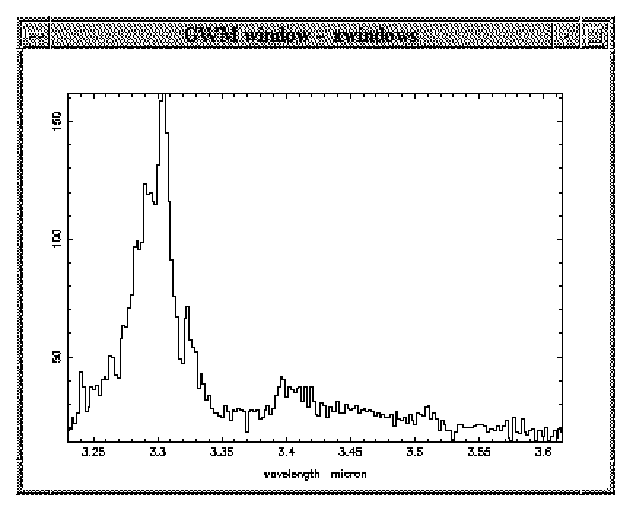
\includegraphics{sun86_spec}
\caption{Example GWM spectrum.}
\end{center}
\end{figure}

   The first command is necessary if your X display `server' is not
   the same as the `client' machine running Figaro for you. It
   passes the remote client the identity of the local server. You have
   to declare `xdisplay' each time you log onto the remote client.

   Conversely, you may also have to reveal the identity of the remote
   client to the local server, say with an `xhost' command. Otherwise
   the remote client may not be allowed use the local server as a
   display.

   The second command tells Figaro which graphics device you want to
   use. `xw' is an abbreviation for `xwindows'. Together with the
   information from `xdisplay' this is sufficient to open the window.
   You should now get a display window on your screen, and a box with
   the word `PGPLOT' in the centre is drawn into the window. You need
   to give the `soft' command only once. Figaro will always remember
   that you want to use the device `xw'.

   The third command finally displays the spectrum contained in the file
   `a\_file.sdf'. Data files can have names ending with `.sdf' or
   `.dst'. They must not contain any additional periods. The Figaro
   commands know about this, and must not be given this file name
   extension.

   Don't worry about the size of this window. By default you get about
   700 by 500 pixels, usually big enough to read the axis labels.

   The word `accept' looks like a parameter to the `splot' command.
   Actually you can use it on any command. It prevents the command from
   prompting you for information that it can guess itself.

   Now consider this more complex sequence of commands. It achieves the
   same thing, basically.

\begin{terminalv}
% xdisplay abc.inter.net
% xmake xwindows -g 400x300 -bg green -fg blue
ICL> splot spectrum=a_file whole=f
XSTART - (XStart) First X-value to be plotted /0.5/ > 3.25
XEND - (XEnd) Last X-value to be plotted /2043.5/ > 3.4
AUTOSCALE - (AUtoscale) Scale so all of spectrum fits? /NO/ > y
LABEL - (LABel) Label for plot /''/ > Plotting a spectrum
HARDCOPY - (HArdcopy) Produce plot as a hard copy? /NO/ >
\end{terminalv}

\begin{figure}[htb]
\begin{center}
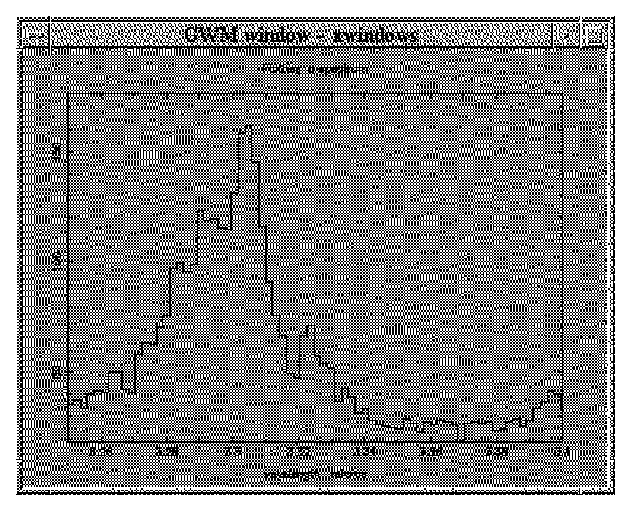
\includegraphics{sun86_spec2}
\caption{A spectrum in a GWM window.}
\end{center}
\end{figure}

   The `xdisplay' command now tells the remote client explicitly what
   the Internet host name of the local server is. This is necessary when
   you log on indirectly, via a third host.

   There is also an extra `xmake' command to create the display window
   explicitly. This way, we can tell it the size and shape of the
   window, and the colours for background and lines. You can make your
   personal preference permanent by specifying resources for `xmake'
   in your `.Xdefaults' file. If you look at the paper copy or on a
   black/white display, you will notice that this is not a good choice
   of colours, since the grey values for blue and green are rather
   similar.

   `xmake' is paired with a command `xdestroy', which you can use to
   get rid of the graphics window. That is necessary before you
   `xmake' it with different parameters, or when you have too many
   windows on your display.

   The `splot' command is different in a number of ways. Before, we had
   given the input data set as the first parameter. When we are not sure
   about the sequence of parameters, we can specify them by name. For
   most Figaro commands that work on spectra as opposed to images, the
   input data are specified in the parameter called `spectrum'.

   Next, we have specified the `whole' parameter as false, so that
   this time we can choose only part of the spectrum to be displayed. We
   also left out the `accept' keyword, that is why the command asks us
   a number of questions while it runs.

%    --------------------------------------------------------------------------

\subsection{\xlabel{lookimag}\label{lookimag}Looking at an image}

%       -----------------------------------------------------------------------

\subsubsection{\label{lookimagimage}The `image' command}

   Suppose you have a data file `a\_file.sdf' with an image, i.e.\ a
   two-dimensional data set and want to plot is on an X display. This is
   one of the most common actions in Figaro. Most users will use the
   `image' command for this purpose. In general it uses a different
   display window than where most other plots go. The idea is that most
   plots are line plots and their device is selected with the command
   `soft'. But `image' should display at least in grey, if not in
   false colours. So you have to specify the imaging device separately,
   although it can be the same actual device as the `soft' device.

   Consider the following sequence of commands:

\begin{terminalv}
% xdisplay
ICL> idev xw
ICL> colour grey
ICL> image a_file accept
\end{terminalv}

   If you are not familiar with the necessities of using X windows over
   the computer network, see
   \latorhtm{Section~\ref{lookspec}.}
   {the section on \htmlref{plotting a spectrum.}{lookspec}}

   The second command tells Figaro which graphics device you want to
   use. `xw' is an abbreviation for `xwindows'. Together with the
   information from `xdisplay' this is sufficient to open the window.
   You should now get a display window on your screen, and a box with
   the words `PGPLOT imaging' in the centre is drawn into the window.
   You need to give the `idev' command only once. Figaro will always
   remember that you want to use the device `xw'.

   The third command changes the display window to show various levels
   of grey as representation of the image data values. A new display
   window may have an undefined `colour lookup table', or a different
   plot command may have changed the lookup table. The `colour'
   command with parameter `grey' always brings it back to normal.

   The fourth command finally displays the image contained in the file
   `a\_file.sdf'. Data files can have names ending with `.sdf' or
   `.dst'. They must not contain any additional periods. The Figaro
   commands know about this, and must not be given this file name
   extension.

\begin{figure}[htb]
\begin{center}
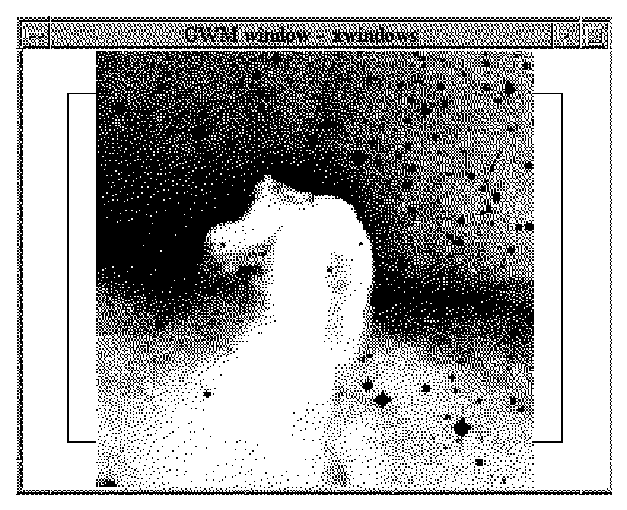
\includegraphics{sun86_imag}
\caption{An example of an image displayed in a GWM window.}
\end{center}
\end{figure}

   The keyword `accept' prevents the command from prompting you for
   information that it can guess itself. Unfortunately, you don't know
   what it did guess, and you might never learn how you can exert more
   control over the display.

%       -----------------------------------------------------------------------

\subsubsection{\label{lookimagadvanced}Advanced use of `image'}

   Now consider this more complex sequence of commands.

\begin{terminalv}
% xdisplay abc.inter.net
% xmake xwindows -g 400x300 -c 128

ICL> image image=a_file prompt
HARDCOPY - Use "hard" devices rather than imaging device /FALSE/ >
IDEV /'xw'/ >
ERASE - Erase screen before display /FALSE/ > t
YSTART - First Y value to be displayed /1/ > min
YEND - Last Y value to be displayed /256/ > max
XSTART - First X value to be displayed /1/ > min
XEND - Last X value to be displayed /256/ > max
LOG - Display using logarithmic scaling /FALSE/ >
OPTIMIZE - Amount of histogram optimisation (0 to 1) /0.5/ > 0
AUTOSCALE - Calculate display limits automatically /TRUE/ >
NEGATIVE - Set limits to give a negative image /FALSE/ > t
XPLACES - Number of sub-displays across screen in X /1/ >
YPLACES - Number of sub-displays across screen in Y /1/ >
ASPECT - Maintain correct aspect ratio for image? /TRUE/ >
IMARRAY /0/ >
IMFILE /''/ >

ICL> image a_file negative=t
ERASE - Erase screen before display /FALSE/ >
YSTART - First Y value to be displayed /1/ > 173
YEND - Last Y value to be displayed /256/ > 191
XSTART - First X value to be displayed /1/ > 94
XEND - Last X value to be displayed /256/ > 117
OPTIMIZE - Amount of histogram optimisation (0 to 1) /0/ >
AUTOSCALE - Calculate display limits automatically /TRUE/ >
XPLACES - Number of sub-displays across screen in X /1/ > 0
XORIGIN - Origin of display in X in display pixels /0/ > 250
YORIGIN - Origin of display in Y in display pixels /0/ > 150
XPIXELS - Number of display pixels to use in X /149/ >
YPIXELS - Number of display pixels to use in X /149/ >
ASPECT - Maintain correct aspect ratio for image? /TRUE/ >
\end{terminalv}

\begin{figure}[htb]
\begin{center}
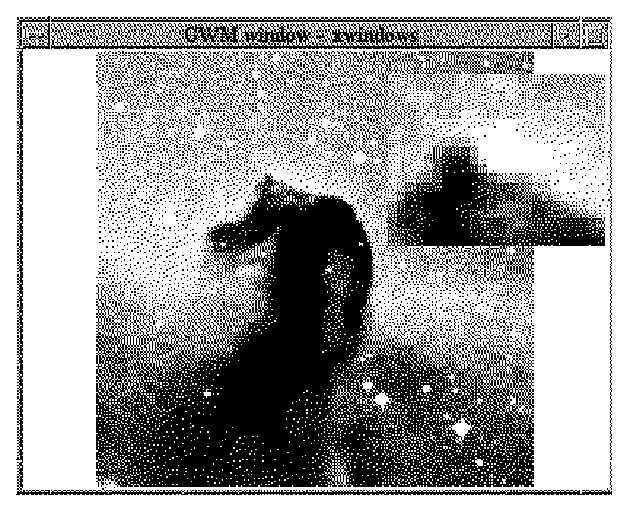
\includegraphics{sun86_imag2}
\caption{Advanced use of the IMAGE command.}
\end{center}
\end{figure}

   If you are not familiar with the necessities of using X windows over
   the computer network, see
   \latorhtm{Section~\ref{lookspec}.}
   {the section on \htmlref{plotting a spectrum.}{lookspec}}


   In the first `image' command the keyword `prompt' is used. While
   `accept' suppresses prompting as far as possible, `prompt' causes
   any command to ask you everything. This is a good way of learning the
   capabilities of commands, but it also causes some spurious prompts
   like the ones for `idev', `imarray', and `imfile'. You should just
   accept the defaults offered for these parameters.

   The first thing we learn through the `prompt' keyword is that `image'
   could have `displayed' to a printer file instead of a screen window.

   We chose to erase the window this time. That gets rid of the
   remainders of the original plain box. Via `ystart'/`yend' and
   `xstart'/`xend' we can select only part of the image to be displayed.
   Since we want the whole image and are not sure about the offered
   default, we use the words `min' and `max'. This time, we set
   `negative' true: The image file contains a negative, negating it
   during display makes is look positive. With `xplaces'/`yplaces' we
   could sub-divide the window into an array of sub-windows and display
   into one of them. We leave `aspect' true so that image pixels are
   displayed as squares. Otherwise the display would be stretched
   horizontally to fill the window.

   Having displayed the whole image, we now run `image' again, but
   display only part of it. We also set `xplaces' zero. That means, we
   can specify the display area in pixels. Since we do not erase this
   time, the previous full display remains partially visible.

%       -----------------------------------------------------------------------

\subsubsection{\label{lookimagcolour}Adding colour}

   While reading
   \latorhtm{Section~\ref{lookimagimage}}
   {the section on \htmlref{the image command}{lookimagimage}}
   you may have wondered
   why the command to choose grey levels is called `colour'. Because
   it can be used to load an existing colour lookup table. This can be
   done before or after `image'. To put some colour into the display
   we already have:

\begin{terminalv}
ICL> colour contour_lut
\end{terminalv}

\begin{figure}[htb]
\begin{center}
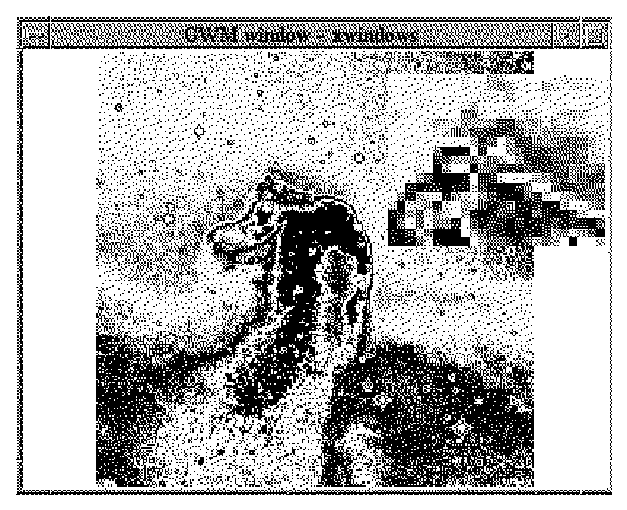
\includegraphics{sun86_imag3}
\caption{Adding color to an image.}
\end{center}
\end{figure}

   There are a number of prepared colour lookup tables. They are
   `.sdf' files, similar to other data files. By convention their
   names end in `\_lut.sdf', and they are stored in a directory pointed
   to by the Unix shell environment variable `FIGARO\_PROG\_S'. To see a
   list of colour tables in that directory:

\begin{terminalv}
% ls $FIGARO_PROG_S/*_lut.sdf
\end{terminalv}
% $

   Finally, how do you prevent line graphics from resetting your image
   display? You will recall that the line graphics device is selected
   with `soft', while the imaging device is selected with `idev'.
   You can simply choose separate windows. Consider this:

\begin{terminalv}
% xmake xwindows -c 16
% xmake xwindows2 -c 128
ICL> soft xw
ICL> idev x2w
\end{terminalv}

   This will separate the output into two windows. There are four
   windows possible, but notice the different names in `xmake' and
   `soft'/`idev'. The `-c' options also reduce the line graphics
   window to the 16 colours reserved for this, and increase the imaging
   window to 128 colours.

%    --------------------------------------------------------------------------

\subsection{\xlabel{lookicont}\label{lookicont}Image display in monochrome}

   If for some reason you cannot use `image' to display images, you
   can still display them as contour plots or as dithered grey plots.
   This works even when the display window has only two colours, say
   when you have a b/w X terminal. Like
   \latorhtm{spectral plots (Section~\ref{lookspec})}
   {\htmlref{spectral plots,}{lookspec}}
   these plots go to the `soft' device.

\begin{terminalv}
ICL> icont a_file min max min max low=0 high=250 contours=6 accept
\end{terminalv}

\begin{figure}[htb]
\begin{center}
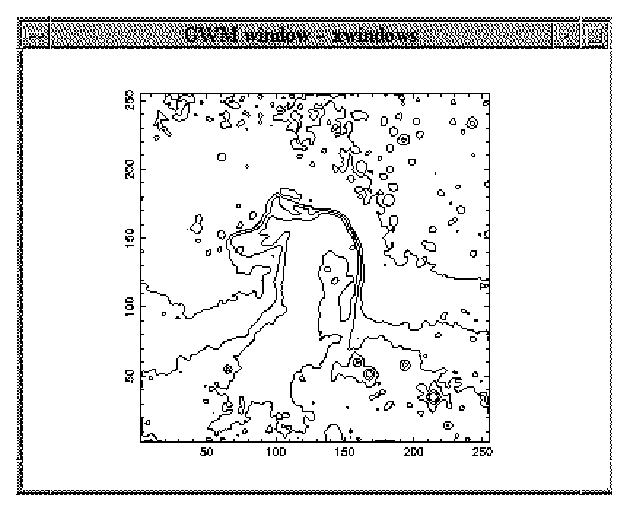
\includegraphics{sun86_icont}
\caption{Using contours.}
\end{center}
\end{figure}

\begin{terminalv}
ICL> igrey a_file min max min max low=0 high=250 accept
\end{terminalv}

\begin{figure}[htb]
\begin{center}
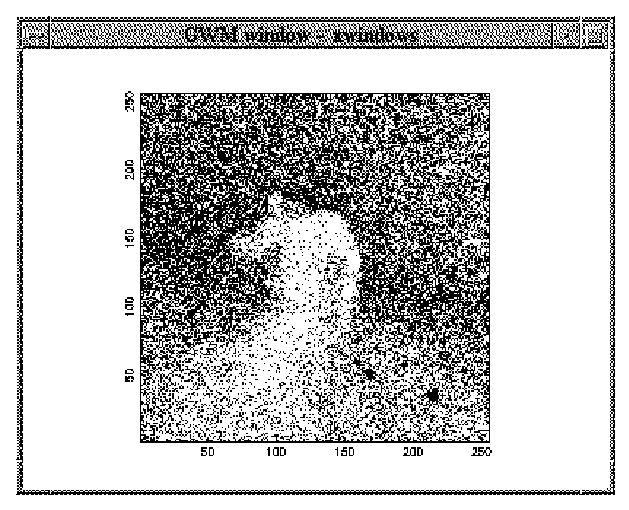
\includegraphics{sun86_igrey}
\caption{Monochrome image.}
\end{center}
\end{figure}

   If the display window has more than 16 colours, `igrey' will use
   those resources and display with true grey levels. It will also reset
   the window colours to grey. Well, strictly speaking the colours are
   not grey, but go linearly from the background colour to the
   foreground colour. If you choose pink and green for fore- and
   background, you can get quite a hideous composition.

%    --------------------------------------------------------------------------

\subsection{\xlabel{hardcopy}\label{hardcopy}Paper copies}

   In order to get paper copies instead of screen plots, you will
   usually use the `hard' device instead of the `soft' device. (Finally
   you understand why it's called the `soft' device!) Similar to the
   commands `soft' and `idev' there is a command `hard' to tell Figaro
   once and for all what your hard-copy device is:

\begin{terminalv}
ICL> hard ps_l
\end{terminalv}

   The main hard-copy devices these days are PostScript
   files\latorhtm{---}{-}files,
   not printers! This means your plots go into a series of files. The
   first is called `gks74.ps', the second is `gks74.ps.1', the third
   ends with `.2', and so on.

   It is a bit difficult to keep track of these files. E.g.\ after you
   created three files you might delete the second. The fourth plot may
   then use the free name and appear to be the second plot. Also, if an
   application erases the graphics device before plotting, you might get
   two files: If you `print' the first, you may just get a blank sheet
   of paper from the printer.

   You can use `ghostscript' (Unix command `gs'; see
   \xref{SUN/197}{sun197}{}) or, more simply, `ghostview' to view the
   plots on the screen before you print the wrong one.  E.g.\ type:

\begin{terminalv}
   ghostview gks74.ps
\end{terminalv}

   There are a number of PostScript devices you can choose from. When
   `hard' prompts for the device, you can try `options' to get a list of
   possible replies. The PostScript devices are:

\begin{itemize}
\item   ps\_l: PostScript, grey, A4, landscape
\item   ps\_p: PostScript, grey, A4, portrait
\item   epsf\_l: Encapsulated PostScript, grey, A4, landscape
\item   epsf\_p: Encapsulated PostScript, grey, A4, portrait
\item   pscol\_l: PostScript, colour, A4, landscape
\item   pscol\_p: PostScript, colour, A4, portrait
\item   epsfcol\_l: Encapsulated PostScript, colour, A4, landscape
\item   epsfcol\_p: Encapsulated PostScript, colour, A4, portrait
\end{itemize}

   Before you get enthusiastic about Colour PostScript, it is not
   possible to use the `colour' application in conjunction with a
   printer device. This is because `colour' would write its own
   PostScript file and the information does not go into the PostScript
   files with the actual display. You need something like KAPPA's
   command `display', which can load a colour table immediately before
   displaying the image. In Figaro the only use for Colour PostScript is
   probably to get coloured line plots where the applications support
   this.

   The difference between the `ps' and `epsf' devices is that the former
   are complete and intended to be sent to the printer. The latter are
   incomplete and intended as elements of more elaborate PostScript
   documents. You could combine several EPSF files into a single
   PostScript file, or you could include EPSF files as figures in a
   \TeX\ or \LaTeX\ document. The figures would be included during
   processing with `dvips'.

   Consider this example:

\begin{terminalv}
ICL> hard epsf_p
ICL> igrey image1 17 23 130 125 hardcopy=t
ICL> icont image2 17 23 130 125 hardcopy=t
% psmerge -e -s0.5x0.5 gks74.ps -s0.5x0.5 gks74.ps.1 > hardcopy.eps
\end{terminalv}

\begin{figure}[htb]
\begin{center}
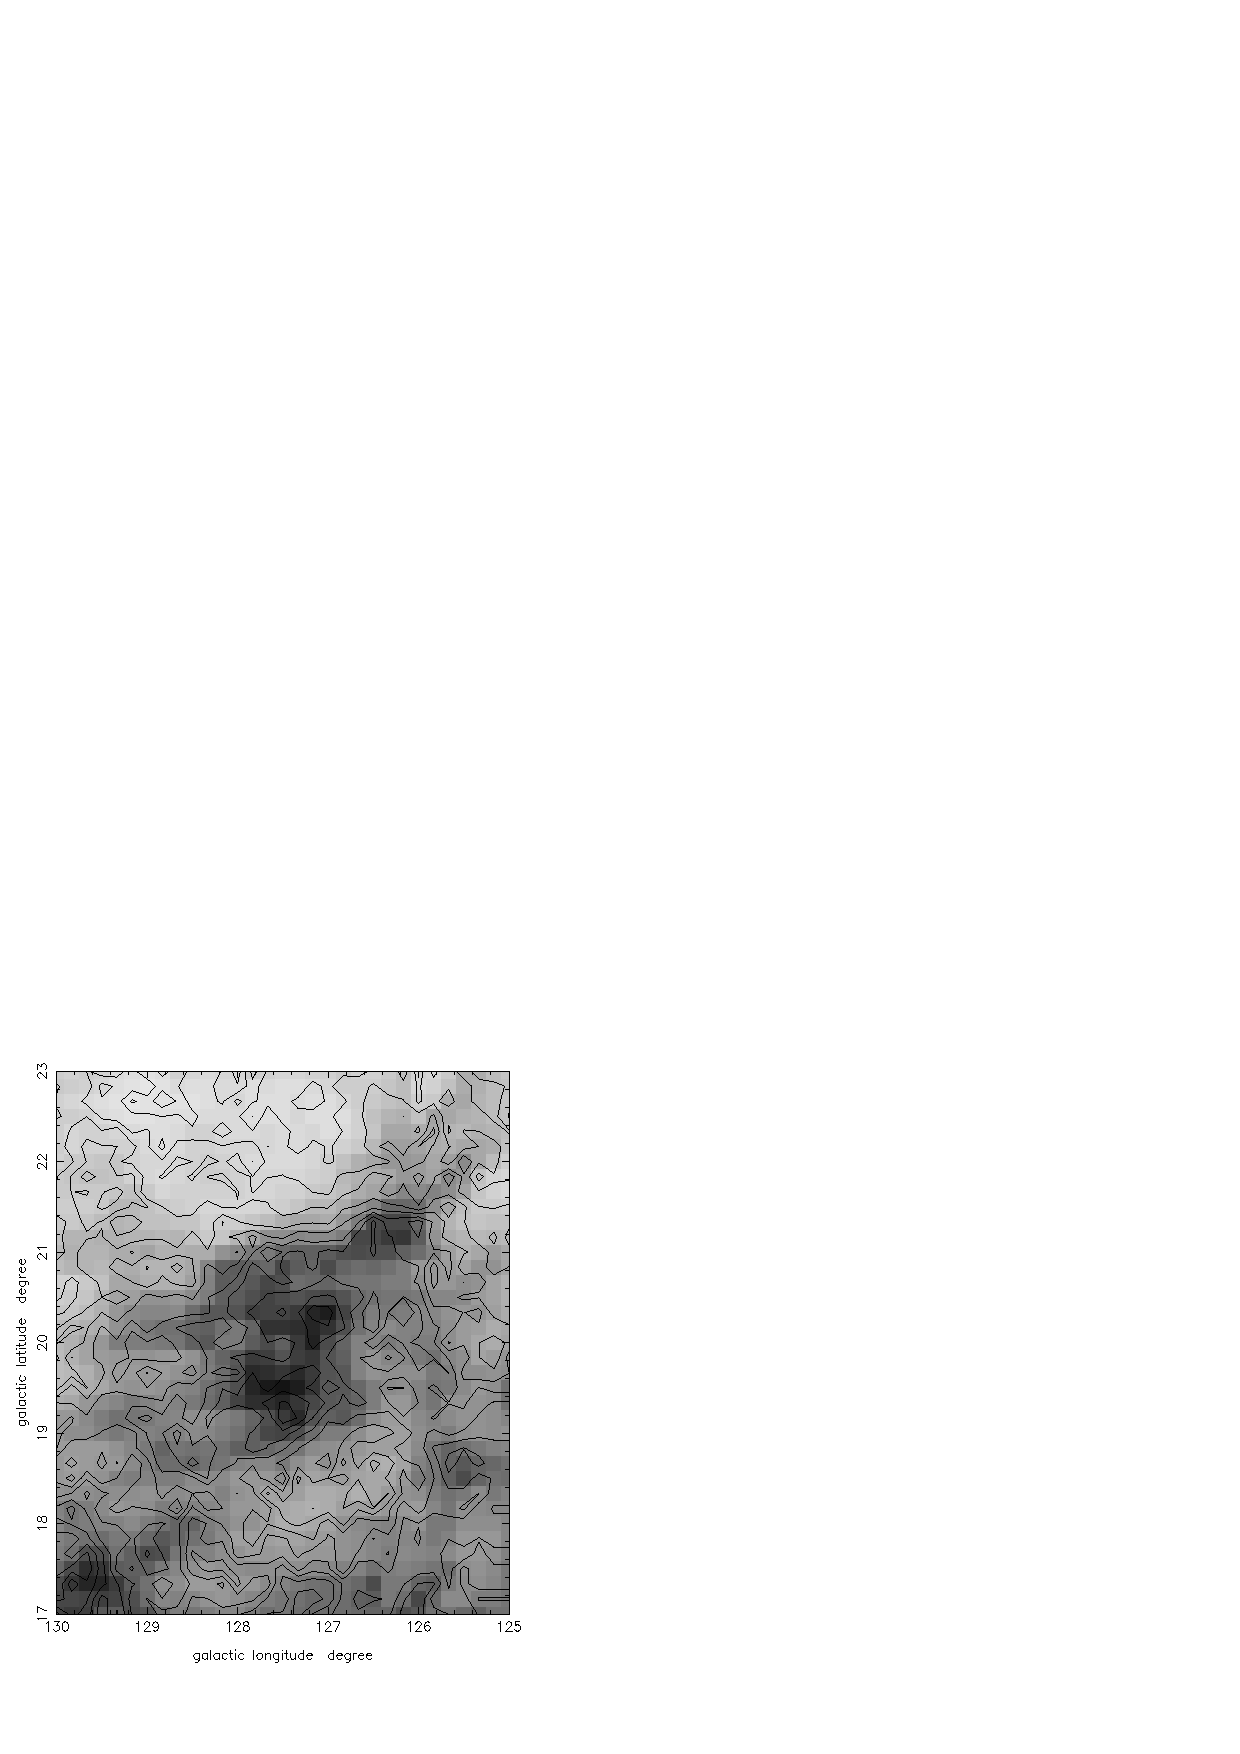
\includegraphics{sun86_hard}
\caption{Postscript output.}
\end{center}
\end{figure}

   We choose the portrait orientation for Encapsulated PostScript. This
   is helpful for later inclusion in a \LaTeX\ document, since it is
   usually printed in portrait orientation as well.

   We use `igrey' and `icont' to produce plots of two images that have
   the same number of pixels per degree on the sky, and we choose the
   same part of the image. The two applications also use the same part
   of the display device. You might be tempted to use this sequence for
   an overlay on the screen, but `icont' will wipe out the plot that
   `igrey' made.

   We use the `hardcopy' keyword to direct the plots to the `hard'
   device rather than the `soft' device. The result are two files
   `gks74.ps*'.

   Instead of printing each on its own piece of paper, we use the
   `psmerge' utility (see \xref{SUN/164}{sun164}{}) to combine the two
   into a single figure.  `psmerge' can not only combine several EPSF
   files, it can also scale, shift and rotate each EPSF graphic
   individually in the process. The `-s' option scales the graphs to half
   the size in $x$\/ and in $y$.

   The `-e' option here means that the output is again EPSF rather than
   PostScript. The idea is that we want to include `hardcopy.eps' in the
   \LaTeX\ version of this document like such:

\begin{terminalv}
   ...style[11pt,epsf]{article}
   ...
   \begin{figure}[htb]
   \begin{center}
   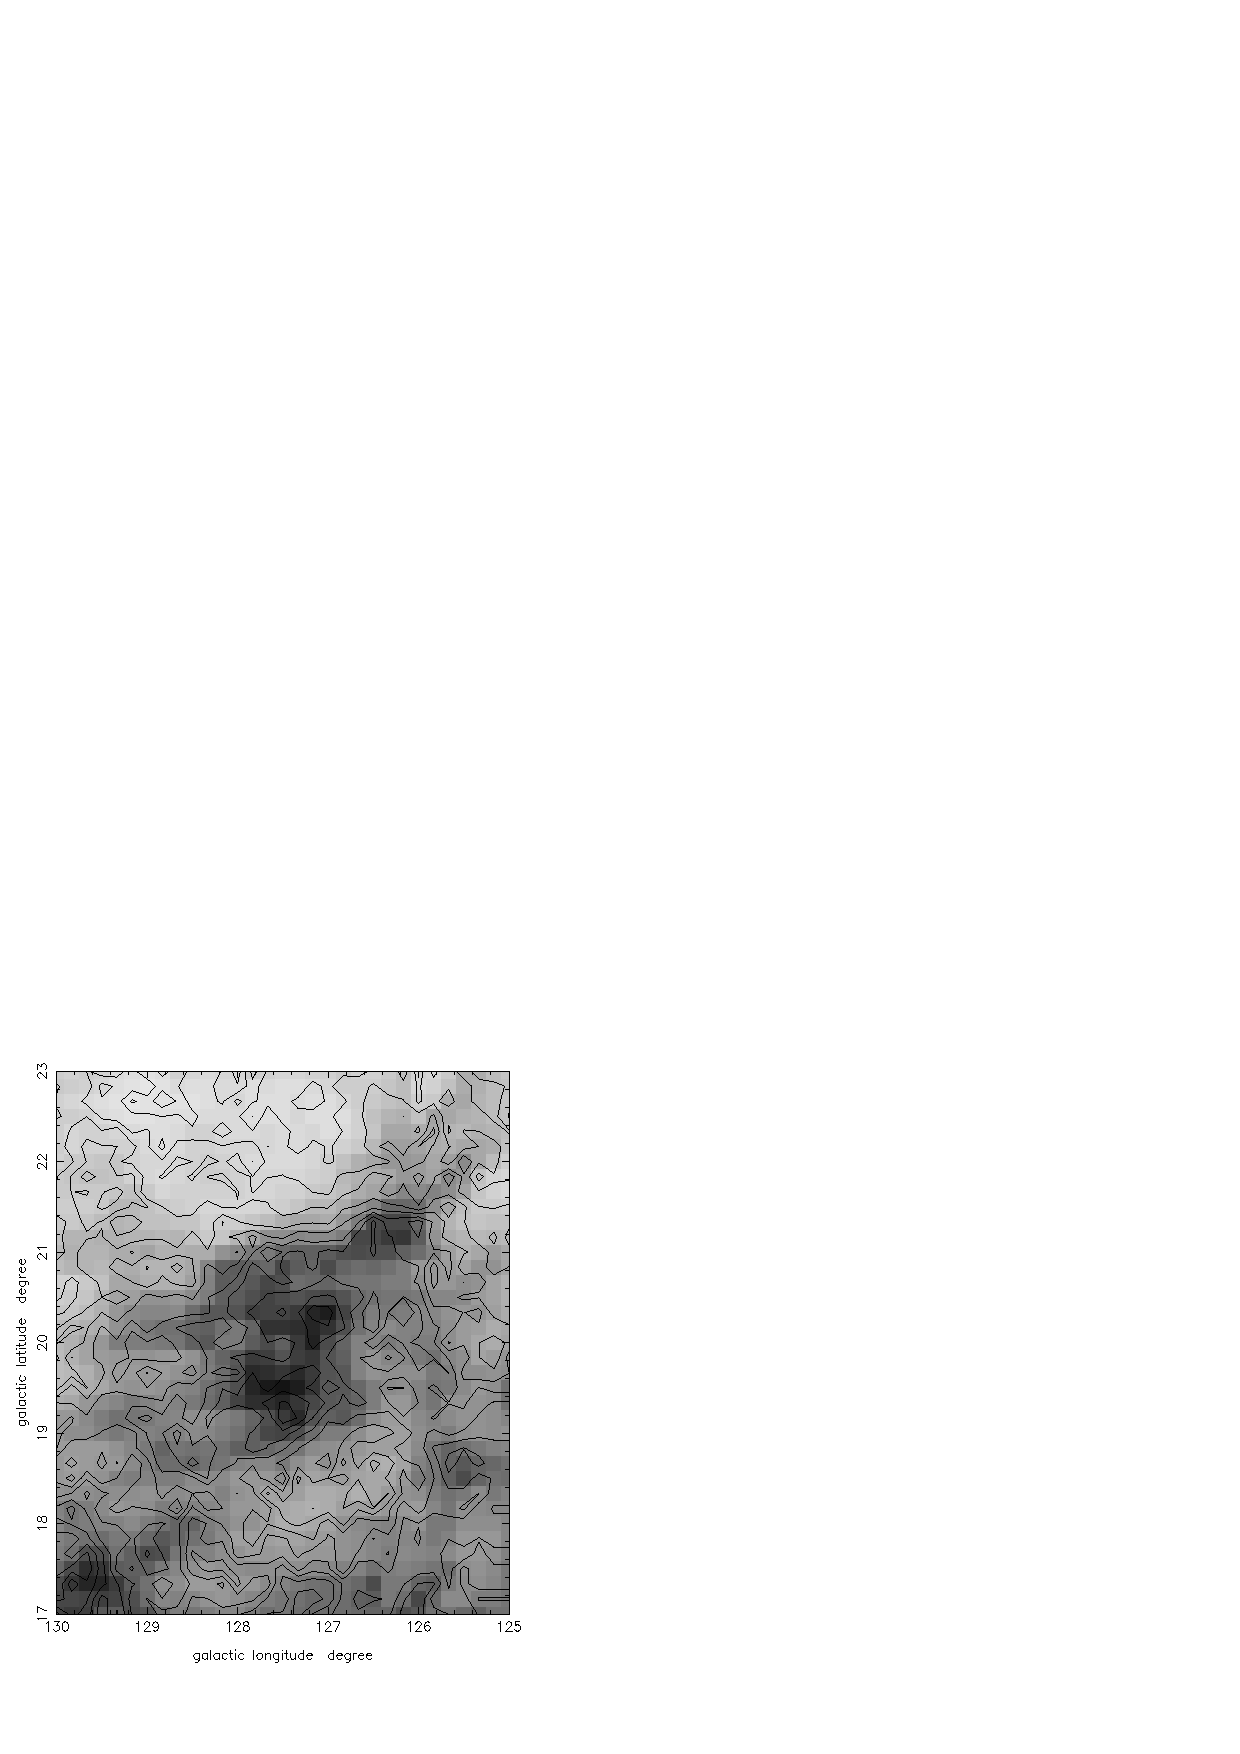
\includegraphics{sun86_hard}
   \end{center}
   \end{figure}
\end{terminalv}

   We are cheating here, because the GKS EPSF files have an unsuitable
   `BoundingBox:'. You have to edit these files and move one line
   from the end of the file to the beginning: There are two lines in the
   EPSF file that begin with `\%\%BoundingBox:'. At the top of the file
   it says `(atend)' and at the bottom of the file it says e.g.\ `0 0 271
   395'. The line at the end must be moved to where the first line is,
   and the first line must be removed. Since PostScript files contain
   plain text, you can use the `vi' editor to do this.

   Also, this BoundingBox is somewhat too large, it contains not only
   the graphic but some white space. You can use `ghostview' to display
   the EPSF file. Its cursor position is constantly displayed, so you
   can move the cursor to the actual corners of the graph and thus find
   out better numbers for the BoundingBox.

   Instead of `igrey', you can used `image' of course to make use of its
   histogram optimisation. You will find it very difficult to align it
   with any contour plot though.

%       -----------------------------------------------------------------------

\subsubsection{Paper copy by cheating}

   Many line plot commands have a `hardcopy' keyword to choose between
   the `soft' and `hard' device, or between the `idev' and `hard'
   device. However, some don't and others use both devices for different
   plots.

   If you actually tried to enter `options' as hard device you will have
   noticed that the list contains the screen devices as well. In fact
   there is no principal difference between all those devices, each can
   be selected as `soft', `hard', or `idev' device. The three commands
   to select the three devices just help Figaro to remember more than
   one device name and to channel the right output to the right device.
   You can send your hard-copies to the X screen and your screen plots
   into a PostScript file!

   This is a valid option. If there is an application that sends your
   favourite plot always to the screen, you can

\begin{terminalv}
ICL> hard ps_l
ICL> soft ps_l draw=f
ICL> idev ps_l draw=f
\end{terminalv}

   and all your plots go into PostScript files. Note that you should use
   the `draw' keyword to suppress the creation of an extra page with the
   frame plotted by `soft' and `idev'.

%    --------------------------------------------------------------------------

\subsection{\xlabel{examine}\label{examine}Examining data}

   If you have
   \latorhtm{displayed an image with `image' (Section~\ref{lookimagimage}),}
   {\htmlref{displayed an image with `image',}{lookimagimage}}
   you can use `icur' to move a cursor over the image. Stop at a point
   of interest, and you can be told the coordinates and data value of
   that point.

\begin{terminalv}
ICL> icur

Use mouse to control cursor.
Press "D" to display pixel data.
Press space bar to record pixel.
Press "Q" to exit.

  76.00000       143.0000       132.3220
  198.0000       184.0000       115.9024
  214.0000       34.00000       3.863415
Pixel record #01 at   167    52   167.0000       52.00000
Pixel record #02 at   155   195   155.0000       195.0000
Pixel record #03 at    61   211   61.00000       211.0000
\end{terminalv}

   On the first three positions `d' was used, on the latter three the
   space bar. `Recording' a pixel does not tell you its brightness, but
   the position is stored for future use.

   If you
   \latorhtm{used `igrey' or `icont' to display, (Section~\ref{lookicont}),}
   {\htmlref{used `igrey' or `icont' to display,}{lookicont}}
   then you can use `igcur' in a similar way to find out about pixels.

   Another useful inspection command is `istat'. It does not need any
   display, but works on the data directly.

\begin{terminalv}
ICL> istat a_file accept

Y-range 1 to 256
X-range 1 to 256
Total (over 65536.0 pixels) = 8.4904E+6
Max   = 246.29   in pixel (89,47)
Min   = 0        in pixel (215,35)
Mean  = 129.55
Sigma = 49.3974
\end{terminalv}

%    --------------------------------------------------------------------------

\subsection{\xlabel{arithm}\label{arithm}Doing simple things}

   With Figaro you can not only look at data that happen to be lying
   around, you can also process data and thus change the contents of
   data files. The simplest operations are adding or subtracting a
   constant, or multiplying or dividing a constant into a data set.
   These four commands are `icadd', `icsub', `icmult', and
   `icdiv'.

\begin{terminalv}
ICL> icadd
IMAGE - (IMage) Name of image to be added to /@a_file/ >
FACTOR - (FACtor) Additive constant /1/ > 25
OUTPUT - (OUTput) Name of resulting image > b_file
\end{terminalv}

   If you compare the statistics of the old `a\_file.sdf' and the new
   `b\_file.sdf', you will find that 25 has been added to each pixel
   value.

   What happens if you give for `output' the same file name as for
   `image'? In most cases this is possible. You will then not get a
   second file, but the first file will be modified to contain the new
   data.

   What if you have a spectrum and not an image? Usually that does not
   matter. When a command asks for the `spectrum' parameter it usually
   has to be a spectrum. But when it asks for the `image' parameter
   you can in most cases give a spectrum instead.

   You can also use two images as operands instead of an image and a
   constant. The commands for this are `iadd', `isub', `imult',
   and `idiv'.

\begin{terminalv}
ICL> idiv
IMAGE - (IMage) Name of first image /@a_file/ >
IMAGE1 - (IMAGE1) Name of second image > b_file
OUTPUT - (OUTput) Name of resulting image > a_file
\end{terminalv}

   The first operand is overwritten with the result.

% -----------------------------------------------------------------------------

\newpage % <<<---
\section{\xlabel{advanced}\label{advanced}Advanced users}


%    --------------------------------------------------------------------------

\subsection{\xlabel{params}\label{params}Parameters: Controlling commands}


%       -----------------------------------------------------------------------

\subsubsection{\label{paramswhatis}What is the parameter system?}

   The applications use the parameter system to get the necessary
   information from the outside world. The source of information is not
   always the user's keyboard. The specification of a parameter on the
   command line is slightly different from entering the value at the
   prompt.

   A good model to imagine the workings of the parameter system is as
   follows.  The system is a pool of parameter values. On the command
   line you can pass values to the parameter system (not the
   application). When the application runs and needs a parameter value,
   it will ask the parameter system (not the user terminal). For each
   parameter the system has two sets of rules, one to arrive at a
   prompt default value and one to work out the value itself. If the
   value was specified on the command line, the system will just pass
   that as the value to the application. Otherwise the value is so far
   unknown to the parameter system and it will construct a prompt
   default and a value according to the rules. There are several
   possible sources for these two:

\begin{itemize}
\item
   the last used value of a global parameter (common to more than one
   application),
\item
   the last used value (as stored on a per-application basis),
\item
   a dynamic default, set by the application at run-time,
\item
   a static default, set in the interface file,
\item
   response to a user prompt.
\end{itemize}

   So asking the user is only one way of getting information from the
   parameter system. You also see that the defaults offered\latorhtm{---}{-}or
   accepted by `accept' on the command line\latorhtm{---}{-}may be arrived
   at in a number of ways.

%       -----------------------------------------------------------------------

\subsubsection{\label{paramsonline}Parameters on the command line}

   There are three useful keywords the user can give on the command line
   to control the defaulting and prompting:

\begin{itemize}
\item
   `accept': Don't prompt, use default values. This is very useful in
   scripts to avoid the script getting stuck at an unexpected prompt.
\item
   `prompt': Prompt for all parameters. This is a good way to find out
   the capabilities of a command.
\item
   `reset': For the prompt default use reset values, instead of last
   used values.
\end{itemize}

   The user is not prompted for a parameter value in all circumstances,
   but a value can be specified on the command line even if it would not
   be prompted for.  Conversely, if a parameter is given on the command
   line, then it will not be prompted for.

   On the command line, parameters can be specified by position or by
   name. To specify by position, they must be in the right order and all
   previous positions must be filled, too. E.g.\ for a spectrum in
   `a\_file.sdf' the following will work:

\begin{terminalv}
ICL> istat image=a_file xstart=min xend=max
ICL> istat a_file xstart=min xend=max
ICL> istat a_file min max min max
\end{terminalv}

   In the third version, the first pair `min max' is for parameters 2
   and 3, `ystart' and `yend'. Although these are not needed for a
   spectrum, positions 2 and 3 must be filled in order to use positions
   4 and 5 for `xstart' and `xend'.

   Logical parameters usually do not have positions assigned to them. On
   the other hand, these can be specified by name and value, or by
   negated name. Consider the `median' parameter of the command
   `istat'. There are two ways to set it true, and two ways to set it
   false:

\begin{terminalv}
ICL> istat median=true
ICL> istat median
ICL> istat median=false
ICL> istat nomedian
\end{terminalv}

   Furthermore, instead of `true', `yes', `t', or `y' can be
   used, similarly with `false' and `no'.

   There are a few vector parameters in Figaro, where the parameter
   value is not a single number but a vector of numbers. To specify
   vector values, use square brackets such as

\begin{terminalv}
ICL> creobj dims=[5,24,3] ...
\end{terminalv}

   If you set the environment variable ADAM\_ABBRV, you can abbreviate
   the parameter names on your command line to the shortest unambiguous
   string. Say `istat' has only one parameter beginning with `i'. Therefore
   `i=a\_file' is just as well as `image=a\_file'.

%       -----------------------------------------------------------------------

\subsubsection{\label{paramsprompt}Prompted parameters}

   When a prompt occurs, it consists of the parameter name, a prompt
   string, and possibly a prompt default. Normally the user responds
   with the value for the parameter. But other responses are possible:

\begin{terminalv}
   PARNAME - Prompt text /Default/ >
   PARNAME - Prompt text /Default/ > \
   PARNAME - Prompt text /Default/ > 123.45
   PARNAME - Prompt text /Default/ > a_file
   PARNAME - Prompt text /Default/ > '1st_file'
   PARNAME - Prompt text /Default/ > @1st_object
   PARNAME - Prompt text /Default/ > min
   PARNAME - Prompt text /Default/ > max
   PARNAME - Prompt text /Default/ > !
   PARNAME - Prompt text /Default/ > !!
   PARNAME - Prompt text /Default/ > ?
\end{terminalv}

   By entering nothing and just hitting return, the prompt default is
   accepted as the proper value. Entering the backslash ($\backslash$)
   accepts the default for this parameter and the respective defaults
   for all parameters that would subsequently be prompted for; no
   further prompting will occur. Sometimes it is necessary to make clear
   that a value is not a number. When a file name begins with a digit
   then in may have to be given with single quotes or with an `at' (@).

   Numeric parameters have a permitted range. The user can ask for
   either of the extreme values to be used by entering `min' or
   `max'. In most circumstances the permitted range of `xstart' etc. is
   the extent of the data in question. The `splot' command is an
   exception: The permitted range is close to the floating point range
   of the machine and grossly exceeds the extent of any reasonable
   spectrum. This is necessary so that you can have a plot that is wider
   than the data reach. `splot' has the logical parameter `whole' to
   adjust the plotted range to the data range itself.

   Entering an exclamation mark should assign the null value to the
   parameter, i.e.\ make the value undefined. In Figaro this has no
   meaning and the application should abort. A double exclamation mark
   is the proper signal for the application to abort. The question mark
   can be used to get
\htmlref{`run-time' help,}{gethelp}
   i.e.\ help on the parameter currently prompted for.

%       -----------------------------------------------------------------------

\subsubsection{\label{paramsoutput}Output parameters}

   Parameters are not only used to pass information \emph{to\/}
   the application, the application may also return information in other
   parameters. `istat' has a number of output parameters in order that
   its results can be used in scripts. From ICL, output parameters can be
   handled quite easily:

\begin{terminalv}
ICL> istat a_file stat_mean=(mean) stat_sigma=(var) accept

Y-range 1 to 256
X-range 1 to 256
Total (over 65536.0 pixels) = 53723.8
Max   = 0.90785  in pixel (89,47)
Min   = 0        in pixel (215,35)
Mean  = 0.81976
Sigma = 0.065904

ICL> print (mean)

0.81976

ICL> var = var * var
ICL> print 'variance = ' (var)

variance =  0.00434334

ICL> ave = sqrt(var)
ICL> print (ave)

0.0659040

ICL> icdiv a_file (mean) ffield
\end{terminalv}

   To achieve anything like that from the Unix shell one needs detailed
   knowledge of the storage of these output parameters in the Unix file
   system. The Unix shell does not have floating point arithmetics, but
   one can at least pass the value from one application to the next:

\begin{terminalv}
% istat a_file accept

   Y-range 1 to 256
   X-range 1 to 256
   Total (over 65536.0 pixels) = 53723.8
   Max   = 0.90785  in pixel (89,47)
   Min   = 0        in pixel (215,35)
   Mean  = 0.81976
   Sigma = 0.065904

% icdiv a_file @$HOME/adam/GLOBAL.STAT_MEAN ffield
\end{terminalv}
% $

   Here it is assumed that the environment variable ADAM\_USER does not
   exist or points to \$HOME/adam.

%       -----------------------------------------------------------------------

\subsubsection{\label{paramssyntax}Syntax conflicts}

   Some confusion arises from syntax conflicts between the Unix shell
   and the ADAM parameter system.

   An instructive example is where the user wants to find out the value
   of a certain pixel in an image. In the language of
   the ADAM parameter system the user is interested in the object
   `a\_file.DATA\_ARRAY.DATA(5,7)':

\begin{terminalv}
ICL> hdstrace a_file.DATA_ARRAY.DATA(5,7)

A_FILE.DATA_ARRAY.DATA(5,7)  <_REAL>
  DATA         152.6
End of Trace.
\end{terminalv}

   Now try the same from the Unix shell:

\begin{terminalv}
% hdstrace a_file.DATA_ARRAY.DATA(5,7)
   Badly placed ()'s.

% hdstrace a_file.DATA_ARRAY.DATA\(5,7\)

   A_FILE.DATA_ARRAY.DATA(5,7)  <_REAL>
      DATA         152.6
   End of Trace.
\end{terminalv}

   As a rule, we have to mask each meta-character with a backslash
   ($\backslash$). The backslashes make
   sure the Unix shell passes the meta-characters on and does not
   interpret them. They then make it through to the ADAM parameter
   system, and from there the previous arguments apply.

   Some people prefer other schemes such as enclosing the whole
   object specification in a pair of single quotes or double
   quotes. The advantage is that you need only two additional
   characters no matter how many pairs of parentheses are in the
   object name. The disadvantage is that you need a matching pair of
   characters, and that sometimes you need to pass quotes to the ADAM
   parameter system.

   The troublesome meta-characters are parentheses \texttt{()}, square
   brackets \texttt{[]}, quotes \texttt{'}, double quotes \texttt{"} and the
   backslash itself.  See \xref{SC/4}{sc4}{} for further details.

%    --------------------------------------------------------------------------

\subsection{\xlabel{files}\label{files}Data files: Internal details}


   Your run-of-the-mill Figaro application uses the NDF library to
   access data. But the HDS object manipulators `copobj', `creobj',
   `delobj', `renobj', `setobj', and `trimfile' use the HDS library to
   access data files, just like `hdstrace' does. Notice the small
   difference between accessing data and accessing data files! The
   point is that two different data formats (NDF and DST) actually use
   the same file format (HDS). Therefore accessing such files on a low
   level is different to accessing the data inside the files on a
   higher level.

%       -----------------------------------------------------------------------

\subsubsection{\label{fileshds}HDS files}

   HDS files play a vital role in Figaro. Two data formats, NDF and
   DST, are realised in HDS files. In addition, the ADAM parameter
   system uses HDS files to store its information. HDS stands for
\emph{Hierarchical Data System,\/}
   and the main feature of HDS files it that there is no fixed order in
   which items are arranged within the files. Instead HDS files contain
   a hierarchy of named objects, all that matters are the hierarchy tree
   and the names of objects, not their sequence.

   The actual information is kept in `primitive' objects. These are
   numbers or strings, scalar or arrays. The other kind of objects are
   structures, which can contain further objects. These are needed to
   build the hierarchy tree. Structures can be arrays, too.

   Users can inspect and modify the contents and organisation of HDS
   files.  For this a syntax to specify objects has been developed.
   To practise the syntax, you can use the `hdstrace' utility (see
   \xref{SUN/102}{sun102}{}) to list the contents of an HDS file:

\begin{terminalv}
ICL> hdstrace a_file full

A_FILE  <NDF>
  DATA_ARRAY     <ARRAY>         {structure}
     DATA(256,256)  <_REAL>         106.2439,126.5268,116.8683,102.3805,
                                 ... 129.4244,134.2537,141.9805,134.2537
End of Trace.
\end{terminalv}

   This shows that the file contains a top-level structure of
   type NDF, within it a structure of type ARRAY called `DATA\_ARRAY',
   and within that a primitive array of type \_REAL called `DATA'. We
   also see that this latter array contains 256 by 256 floating point
   numbers.

   You do not have to inspect the whole file, but can concentrate on
   specific objects within the object tree. For this you use the
   component names and dots between them. To address array elements,
   use parentheses:

\begin{terminalv}
ICL> hdstrace @"a_file.sdf".DATA_ARRAY.DATA(2,1)

A_FILE.DATA_ARRAY.DATA(2,1)  <_REAL>
  DATA         126.5268
End of Trace.
\end{terminalv}

   Here the @ and the double quotes are not necessary, but they show
   how you can address a DST file instead. The double quotes bind the
   `.sdf' into the file name so that it does not look like the object
   `SDF' within the file. The @ makes clear that you talk about an HDS
   object and not a string or a number. An @ may be useful if you have
   file names that begin with a digit.

   The top-level object is equivalent to the file itself and is not
   specified. Its name is in fact irrelevant, so long as it is a
   scalar structure. The other object names are case-insensitive, you
   can use upper case as in the example, or lower case.

   HDS files have names ending with the file name extension `.sdf',
   which stands for Starlink Data File. But this does not have to be so.
   Figaro's second data format, DST, also uses HDS files, but their
   names end in `.dst'. You could use any file name extension, `.sdf'
   is just the default that is assumed if you don't specify it, such
   as:

\begin{terminalv}
ICL> hdstrace @"a_file.dst".Z.DATA(2,1)

A_FILE.Z.DATA(2,1)  <_REAL>
  DATA         126.5268
End of Trace.
\end{terminalv}

   A remark is necessary about data types here. The primitive data
   types (those that do not make HDS structures, but scalars, vectors
   and arrays of numbers, strings, etc.) have names beginning with an
   underscore. The most common type is `\_REAL', others are
   `\_DOUBLE', `\_INTEGER', `\_BYTE', `\_UBYTE', and `\_CHAR*n'. When
   an HDS structure manipulator needs to be given a type, then these
   are to be used. But if a data processing application such as
   `retype' needs a type specification, then you have to use the
   traditional Figaro type specifications `FLOAT', `DOUBLE', `INT',
   `BYTE', and `CHAR'.

%       -----------------------------------------------------------------------

\subsubsection{\label{filesndf}NDF format}

   NDF, the
\emph{Extensible N-Dimensional Data Format,\/}
   is a data format for spectra, images, cubes etc. In the first place
   this is a specification of an HDS object hierarchy. Although
   Figaro's old data access routines (DSA/DTA) did a reasonably good
   job at implementing the NDF format, Figaro now uses the official
   implementation in the form of the NDF subroutine library.
   So the term `NDF' is not only a recipe for an HDS object tree, it
   is also the name of a subroutine library to create and access such
   a tree. And it is customary to call a data set in NDF format `an
   NDF'.

   The minimum content of an NDF is an object with name
   `DATA\_ARRAY'. It must either be a `primitive' array (one that
   contains numbers etc.), or it must be a structure of type `ARRAY' and
   contain a primitive array called `DATA'. The two variants are
   called a primitive NDF and a simple NDF. The following two are
   equivalent, the first is simple, the second is primitive:

\begin{terminalv}
   A_FILE  <NDF>
      DATA_ARRAY     <ARRAY>         {structure}
         DATA(256,256)  <_REAL>         106.2439,126.5268,116.8683,102.3805,
                                     ... 129.4244,134.2537,141.9805,134.2537
   End of Trace.

   A_FILE  <NDF>
      DATA(256,256)  <_REAL>         106.2439,126.5268,116.8683,102.3805,
                                  ... 129.4244,134.2537,141.9805,134.2537
   End of Trace.
\end{terminalv}

   The difference can normally be ignored, since the software will sense
   which variant is present and act accordingly.  When you have to
   specify HDS objects to `hdstrace', `creobj' etc, you must of course
   check which variant is present.  Simple NDFs are more flexible, and
   are also the standard variant.

   There are a number of further components in addition to the data
   array that an NDF can have. There may be a variance array of the same
   shape as the data array, or title, label and unit strings. A
   relatively complete NDF might look like this:

\begin{terminalv}
A_FILE  <NDF>

   TITLE          <_CHAR*32>      'krypton singlet'
   UNITS          <_CHAR*32>      'A/D numbers per exposure'
   LABEL          <_CHAR*32>      'OBJECT - DARK'

   DATA_ARRAY     <ARRAY>         {structure}
      DATA(310,19)   <_REAL>         1655.552,1376.111,1385.559,1746.966,
                                     ... 1513.654,1465.343,1446.902,0,0,0,0,0
      BAD_PIXEL      <_LOGICAL>      FALSE

   VARIANCE     <ARRAY>           {structure}
      DATA(310,19)   <_REAL>         87.05064,21.38796,1.088109,14.45454,
                                     ... 286.3985,132.1791,119.0586,0,0,0,0,0

   QUALITY        <QUALITY>       {structure}
      BADBITS        <_UBYTE>        *
      QUALITY(310,19)  <_UBYTE>      0,0,0,0,0,0,0,0,0,0,0,0,0,0,0,0,0,0,
                                     ... 0,0,0,0,0,0,0,0,0,0,0,0,0,0,*,*,*,*,*

   AXIS(2)        <AXIS>          {array of structures}
   Contents of AXIS(1)
      UNITS          <_CHAR*32>      'microns'
      LABEL          <_CHAR*32>      'Estimated wavelength'
      DATA_ARRAY     <ARRAY>         {structure}
         DATA(310)   <_REAL>            1.85115,1.852412,1.853675,1.854938,
                                        ... 2.237606,2.238869,2.240132,2.241395
   Contents of AXIS(2)
      DATA_ARRAY     <ARRAY>         {structure}
         DATA(19)    <_REAL>         0.5,1.5,2.5,3.5,4.5,5.5,6.5,7.5,8.5,
                                     ... 12.5,13.5,14.5,15.5,16.5,17.5,18.5

End of Trace.
\end{terminalv}

   The most remarkable addition, and quite commonly present, is the
   AXIS. AXIS is an array of structures, even if the data are
   one-dimensional. Each element AXIS(1), AXIS(2) ... is thus a
   structure. In fact, it is very similar to a minimal NDF. In the AXIS
   each pixel is given its own coordinate value. In general
   AXIS(i).DATA\_ARRAY.DATA need neither be linear nor monotonic.
   However, most software may assume one or the other.

   There are a few cases where Figaro treats NDFs differently from other
   Starlink packages.  The details are as follows.

\begin{itemize}
\item
   In Figaro the variance array must not contain bad values. `goodvar'
   can be used to clean up an offending data set.
\item
   Figaro ignores an origin different from (1,1,...).
   The origin is the number of the first pixel. It can specify that the
   first pixel should be counted as pixel 5, or -10, etc. In simple NDFs
   the origin can be stored, but Figaro will not use such
   information. As far as it is concerned all data sets begin with
   pixel (1,1,...). The \xref{KAPPA}{sun95}{} package has an
   application `\xref{setorigin}{sun95}{SETORIGIN}' that allows you to
   adjust the origin.
\item
   Some Figaro applications may assume that an absent AXIS is
   equivalent with pixel coordinates 1.0, 2.0, 3.0, ...
   The default pixel coordinates are in fact ORIGIN-0.5,
   ORIGIN+0.5, ORIGIN+1.5, ...
   Sometimes this NDF default is manifested as an actual axis
   data array, in which case applications may no longer recognise it as
   a default. For the first and second axes you can use `lxset' and
   `lyset' to give the data new pixel coordinates.
\end{itemize}

%       -----------------------------------------------------------------------

\subsubsection{\label{filesndfsect}NDF sections}

   A great advantage in accessing data via the NDF library is that you
   can specify a section of the data rather than the full array.
   The section can specify a part of the array, or it might only
   partially overlap with the array, or they might not overlap at
   all. The section can also have a different
   dimensionality than the array itself. Here is an example
   specification of a seven-dimensional section, in each dimension a
   different feature of the section specification syntax is used:

\begin{terminalv}
% istat file(3:5,21.3:44.5,17,17.0,3:,,:99)

   # (3:5,           1st axis: pixels 3 through 5
   #  21.3:44.5,     2nd axis: pixel centre values 21.3 through 44.5
   #  17,            3rd axis: pixel 17 only
   #  17.0,          4th axis: only the pixel with centre = 17.0
   #  3:,            5th axis: pixels 3 through end of NDF
   #  ,              6th axis: all pixels
   #  :99)           7th axis: pixels from start of NDF through to pixel 99
\end{terminalv}

   The commas separate the dimensions (axes) from one another. Colons
   mean that there's a range rather than a single value. If the start
   or end of a range is left out, the start or end of the NDF is
   used. Integer numbers are pixel indices, floating point numbers are
   pixel centre values (e.g.\ wavelengths). Instead of using a colon
   to separate start and end, you can also use a tilde to separate the
   centre of the section from the size of the section.

   You can use NDF sections whenever existing data are accessed. You
   cannot use NDF sections to specify output data. And you cannot use
   NDF sections when access is to the HDS file rather than the data
   inside it.

%       -----------------------------------------------------------------------

\subsubsection{\label{filesndfforeign}Foreign formats}

   Another great advantage of using the NDF library for data access is
   that data need not be in NDF format. Any foreign data format can be
   accessed, so long as a conversion to NDF is defined. An easy way to
   define a large number of format conversions is to start up the
   CONVERT package in addition to Figaro:

\begin{terminalv}
ICL> convert

CONVERT commands are now available -- (Version 0.6-2, 1996 September)

Defaults for automatic NDF conversion are set.

Type conhelp for help on CONVERT commands.
\end{terminalv}

   At the time of writing this is the list of file name extensions and
   formats. The list is in order of preference of the formats.

\begin{terminalv}
.sdf     NDF format
.fit     FITS format (disk FITS, IBM byte order)
.dst     Figaro format
.imh     IRAF format
.hdr     GASP format
.unf     unformatted binary files
.dat     unf0 binary files
.asc     ASCII files
.txt     text files
.gif     GIF images
.tif     TIFF images
.sdf.Z   compressed NDF files
\end{terminalv}

   Normally you need not concern yourself with the file name
   extension. The data access routines will go through the list and
   give the application the first data set found no matter which
   original format they are in. But if you want to be specific, you
   can say

\begin{terminalv}
ICL> istat file.fit(3:5,21.3:44.5,17,17.0,3:,,:99)
\end{terminalv}

   if you want to use the disk-FITS file when there is also a
   `file.sdf' lying around on your disk. As you can see, you can even
   use \htmlref{NDF sections}{filesndfsect} on foreign data formats.

   You can use foreign formats whenever data are accessed, be it input
   or output. You cannot use foreign formats when access is to an HDS
   file rather than to data. Things like `delobj' can be used only on
   HDS files, which restricts it to NDF and DST format.

   Whether you can actually store your data in a foreign format, is
   not guaranteed. Figaro occasionally uses a FITS extension, which you
   would lose if you store data in GIF. More relevant is that NDF and
   DST formats allow you to have non-linear pixel centre coordinates,
   and you are likely to lose such coordinates altogether if you store
   in FITS or IRAF format.

   There is a penalty for using foreign formats rather than NDF.
   Accessing input and releasing output data takes that bit longer to
   do the format conversion. And it may take a lot longer if the disk
   is not local to the computer that does the processing. So if you
   use only Figaro and other Starlink packages, it is best to stick
   with NDF format. If every third application you use is from IRAF
   or MIDAS, you might be better off using disk-FITS.

   NDF to ASCII and ASCII to NDF conversions can also be performed
   using the ex-SPECDRE applications ASCIN and ASCOUT. ASCIN will
   read axis values, pixel widths, data values, and data errors from
   an ASCII table into an NDF structure, while ASCOUT will create
   such an ASCII table from an NDF.

   For more information on foreign formats see the Developer's Guide
   on adding format conversion to NDF \xref{(SSN/20)}{ssn20}{}
   and the user documentation on CONVERT \xref{(SUN/55)}{sun55}{}.

%       -----------------------------------------------------------------------

\subsubsection{\label{filesdst}DST format}

   One of the foreign formats is called the `Figaro format'\latorhtm{---}{-}in
   fact it is Figaro's old DST format. These days Figaro uses NDF format,
   but that was the case only since version 3.0.

   Like NDF, DST is a specification of an HDS object hierarchy. Only the
   hierarchy is different, the same information is in different places.

   The NDF shown in \latorhtm{Section~\ref{filesndf}}
   {the section on the \htmlref{NDF format}{filesndf}}
   would look in DST format like this:

\begin{terminalv}
A_FILE  <FIGARO>

   Z              <IMAGE>         {structure}
      UNITS          <_CHAR*32>      'A/D numbers per exposure'
      LABEL          <_CHAR*32>      'OBJECT - DARK'
      FLAGGED        <_LOGICAL>      TRUE
      DATA(310,19)   <_REAL>         1655.552,1376.111,1385.559,1746.966,
                                     ... 1513.654,1465.343,1446.902,*,*,*,*,*
      ERRORS(310,19) <_REAL>        9.330093,4.624712,1.043125,3.801913,
                                     ... 16.92331,11.49692,10.9114,0,0,0,0,0

   X              <AXIS>          {structure}
      LABEL          <_CHAR*32>      'Estimated wavelength'
      UNITS          <_CHAR*32>      'microns'
      DATA(310)      <_REAL>         1.85115,1.852412,1.853675,1.854938,
                                     ... 2.237606,2.238869,2.240132,2.241395

End of Trace.
\end{terminalv}

   DST stores errors instead of variances. There is no `a\_file.Y'
   structure, since the second axis has default pixel coordinates. In
   DST format only non-default axes must actually exist.

   There is also no quality array, instead the data array has bad values
   interspersed with good values. This is not a property of the DST
   format itself, but the way the format conversion treats a quality
   array.

%       -----------------------------------------------------------------------

\subsubsection{\label{filesextens}Figaro Extension to NDF and DST structures}

   Due to the flexibility of HDS object trees, it is possible to add
   extra information. Usually such information is recognised only by
   specific software. In the NDF format, Figaro uses a Figaro extension
   and a FITS extension. Any extension to an NDF is an object within a
   `MORE' structure. Since axes are also kind-of NDFs, they can have
   extensions, too. Figaro is probably the only package to use an
   extension to axes.

   In DST format the information that would be in NDF extensions is not
   so obvious to locate. The following table translates between objects
   in an NDF extension and the equivalent in a DST file.

\begin{center}
\begin{tabular}{rl}
DST & NDF \\ \hline
\texttt{.FITS}       & \texttt{.MORE.FITS} \\
\texttt{.OBS.TIME}   & \texttt{.MORE.FIGARO.TIME} \\
\texttt{.OBS.SECZ}   & \texttt{.MORE.FIGARO.SECZ} \\
\texttt{.Z.MAGFLAG}  & \texttt{.MORE.FIGARO.MAGFLAG} \\
\texttt{.OBS.OBJECT} & \texttt{.TITLE} \\
\texttt{.Z.RANGE}    & \texttt{.MORE.FIGARO.RANGE} \\
\textit{.extra}      & \texttt{.MORE.FIGARO}\textit{.extra} \\
\end{tabular}
\end{center}

% Original version of the above table:
%
% \begin{terminalv}
%   DST           NDF
%  ------------- ----------------------
%   .FITS         .MORE.FITS
%   .OBS.TIME     .MORE.FIGARO.TIME
%   .OBS.SECZ     .MORE.FIGARO.SECZ
%   .Z.MAGFLAG    .MORE.FIGARO.MAGFLAG
%   .OBS.OBJECT   .TITLE
%   .Z.RANGE      .MORE.FIGARO.RANGE
%   .<extra>      .MORE.FIGARO.<extra>
% \end{terminalv}

   The FITS extensions in the two formats differ internally. In DST each
   FITS item is an HDS object. But in NDF format the whole FITS header
   is an array of strings, and each FITS item is a string in this array.

   Needless to say, all but the FITS extension go overboard when
   you use other foreign data formats. You can inspect the FITS
   extension with `fitskeys' and add or change items with `fitset'.

%    --------------------------------------------------------------------------

\subsubsection{\label{specextens}\xlabel{extension}The Specdre Extension}

   The
\xref{NDF data access routines}{sun33}{}
   -- together with the lower-level
\xref{HDS routines}{sun92}{}
   -- allow the construction of extensions to the data format.
   Extensions unknown to an application package are propagated, and
   extensions known to an application enable it to provide more
   functionality.

   The Specdre applications use a set of extensions to the basic NDF
   format to communicate information between themselves.  This
   extension is known (not unreasonably) as the \htmlref{\textbf{Specdre
   Extension}}{specdreextens}.  It is recognised and understood by all the
   Specdre applications.  Other Figaro applications, and applications
   in other Starlink packages such as KAPPA, simply propagate the
   Specdre extension unchanged without modifying (or understanding) it.
   This behaviour is not always correct, but in general it is the best
   that can be done.  If the dataset is not processed with another
   Specdre application it does not matter if the Specdre extension and
   the basic NDF become inconsistent (because other applications will
   ignore the extension).  If a Specdre application is presented with
   a dataset in which the Specdre extension is obviously inconsistent
   with the basic NDF it will notice and report an error.

   Specdre contains a number of subroutines for easy and consistent
   access to the Extension. Programmers are advised to contact the
   Figaro support username (e-mail \texttt{figaro@star.rl.ac.uk}) if they want
   to make use of the Specdre Extension in their programs.

   All Specdre applications support version 0.7 of the Specdre
   Extension, which was introduced in version 0.7 of Specdre. Some
   applications support an advanced version 1.1 of the Extension, as
   introduced in version 1.1 of the package.

%    --------------------------------------------------------------------------

\paragraph{Design}

   The spectroscopic axis information is not quite complete with only
   label and units in the axis structure. For a frequency scale you have
   to know which reference frame it refers to, for wavelengths you might
   also be worried about the refractive index of the medium in which the
   wavelength is measured. And for radial velocity scales you need to
   know the rest frequency of the spectral line. Another thing most
   useful in spectroscopy would be to store continuum and line fits
   along with the data. The concept of
\xref{extensions to an NDF}{sun33}{extensions}
   provides a
   good means to store such information. The design of Specdre's own
   extension is outlined here.

   The Specdre Extension is the structure \texttt{<myndf>.MORE.SPECDRE} and
   is of type \texttt{SPECDRE\_EXT}. \texttt{<myndf>} is the creation name of
   the main NDF, the one with the data, axes etc. \texttt{<myndf>.MORE}
   contains all the extensions to this main NDF. The Specdre Extension
   may \textit{contain} other NDFs, thus we have to distinguish between the
   ``main NDF'' and the ``Extension NDFs''.

%    --------------------------------------------------------------------------

\paragraph{\label{specdreextens}\xlabel{specdreextens}Using the Specdre Extension}

   The demonstration script (\texttt{demo\_specdre}) shows the use of the
   Specdre Extension.  There is a tool
\texttt{\htmlref{editext}{EDITEXT}} to look at or manipulate the
   Extension. \texttt{resamp} will usually store some limited amount of
   information about the interdependence of post-resample pixels in the
   Extension. If you try to \texttt{fitgauss} such re-sampled data, that
   application will pick up and use the information in the Extension.

\texttt{\htmlref{fitgauss}{FITGAUSS}}
   or
\texttt{\htmlref{fitpoly}{FITPOLY}}
   will store their fit results in the Extension. In conjunction with
   the NDF sections
(see Sections~\ref{filesndfsect} and \ref{specdreslice})
   you can work your way through the rows of a CCD long-slit spectrum,
   store each row's fit in the Extension and fill the result storage
   space. The collection of all fits is again an NDF (located in the
   Extension) and can be fed into other applications like \texttt{specplot}, \texttt{ascout}, or indeed KAPPA's
\texttt{\xref{display}{sun95}{DISPLAY}}.

   The Extension also provides a place to store a full-size array for
   the wavelength or frequency etc.\ of each pixel.  This array of
   spectroscopic values may be created by \texttt{grow}, and is used by \texttt{arcdisp} to apply individual dispersion curves for the rows of an image.
   The image may be a long-slit spectrum, or the rows may be extracted
   fibre spectra or \'echelle orders.

   There is some potential for confusion here.  You may tend to count
   pixels in your data starting at 1, you may use NDF pixel indices, NDF
   pixel coordinates, a vector of pixel centre values, or an
   N-dimensional array of spectroscopic values.

\begin{itemize}
\item \textit{Pixel indices} along an axis in an NDF are counted from the
   \textit{lower bound} to the \textit{upper bound}.  The lower bound is also
   known as the \textit{origin}.  It is not necessarily 1.  Say, if an NDF
   has bounds 1 ... N, a section of it may have bounds 5 ... (N-6), or
   -5 ... (N+6) etc.  If the section is made permanent in a new file, it
   will still have origin other than 1.  Usually it is these pixel
   numbers -- or the section bounds -- that are used to specify NDF
   sections in parameter values like \texttt{ndf(-25:32,4:)}.

\item The centres of pixels in an NDF have \textit{pixel coordinates} that
   are the pixel number minus 0.5.  So if the bounds are 5 ... 95 then
   the pixels have centre coordinates 4.5 ... 94.5.  The beauty of
   these coordinates is that, if you give each pixel an extent of
   0.5 on either side, then the sequence of pixels 1 .... N cover the
   coordinate range [0;N].  These are only default coordinates, but
   they are worth mentioning because they are similar, but not equal, to
   the pixel indices.

\item Each axis of the NDF may have an explicit vector with the
   coordinates of the pixel \textit{centres}.  These can run non-linear,
   backwards, or in loops.  You may find that some software cannot cope
   with the weirder of these options.  These \textit{centres} can be used
   to specify NDF sections.  You simply give a floating point bound
   instead of an integer bound.  Note that this works only because each
   axis has a \textit{vector} of pixel centres as long as the NDF axis, not
   an N-dimensional \textit{array} of pixel centres.

\item For Specdre it is useful to have \textit{in addition} an
   N-dimensional array where for example a wavelength calibration can be
   stored for each row of an image or a cube individually.  For this
   purpose there may exist an array of \textit{spectroscopic values} in the
   Specdre Extension to the main NDF.  That array is an NDF with the
   same bounds as the main NDF.  Where the main NDF stores the count
   rate, brightness etc.\ of a pixel, the spectroscopic values' NDF
   stores the wavelength, frequency, radial velocity etc.\ for that
   pixel.  This information is recognised only by Specdre.  You cannot
   expect KAPPA's \texttt{linplot} to use it for axis labelling, Specdre's
   \texttt{specplot} does use it of course.  You also cannot use this array
   to specify an NDF section in a parameter value.

\item There is no rule as to what happens to the \textit{centres} of the
   spectroscopic axis when N-D \textit{spectroscopic values} are created or
   modified.  Both arrays may lead rather independent lives.
\end{itemize}

% -----------------------------------------------------------------------------

\paragraph{Specdre Extension v.\,0.7}

   The items of the Extension as introduced with Specdre version 0.7 are
   described below. All top-level items are optional, but each is either
   complete or absent.

\begin{itemize}

\item\texttt{.SPECAXIS} is an \_INTEGER scalar which defaults to 1. Its
   value is the number of the spectroscopic axis. This is the axis along
   which the one-dimensional `spectroscopic subsets' extend. It must
   be greater than or equal to 1 and less than or equal to the number of
   axes in \texttt{<myndf>}. A change of \textit{specaxis} may render other
   components invalid as regards their values or shapes.

\item\texttt{.RESTFRAME} is a \_CHAR*32 scalar which defaults to
   `unknown'.  Its value describes the rest frame used to express the
   observed frequency, wavelength, radial velocity, or redshift.

\item\texttt{.INDEXREFR} is a \_REAL or \_DOUBLE scalar which defaults to
   1. Its value is the index of refraction needed to convert frequency
   into wavelength and vice versa.

\item\texttt{.FREQREF} is a \_REAL or \_DOUBLE scalar which defaults to the
   bad value. Its value is the reference frequency needed to convert
   between radial velocity and redshift on the one hand and frequency on
   the other hand. The value is evaluated together with \texttt{.FREQUNIT}:

   \[\nu_0=\textit{freqref}*10^\textit{frequnit}*{\rm Hz}\]

\item\texttt{.FREQUNIT} is an \_INTEGER scalar which defaults to 0. Its
   value is the common logarithm of the unit used for \texttt{.FREQREF}
   divided by Hertz.  Note that this item is not of type \_CHAR, \_REAL
   or \_DOUBLE.

\item\texttt{.SPECVALS} is an NDF structure with data, label and units
   components. \texttt{.SPECVALS.\-DATA\_\-ARRAY} is a \_REAL or \_DOUBLE
   array which has the same shape as \texttt{<myndf>}. It defaults to a
   multiple copy of the centre array of the spectroscopic axis \texttt{<myndf>.AXIS\-(\textit{specaxis})\-.DATA\_\-ARRAY}. This structure
   contains spectroscopic axis values (either wavelength, or frequency,
   or velocity, or redshift) for each pixel of the data cube. Labels and
   units must be stored with this data structure. Their default values
   are copies from the spectroscopic axis \texttt{<myndf>.AXIS(\textit{specaxis}).LABEL, .UNITS} in the main NDF or `unknown' if the axis
   has no label or unit. A modification of spectroscopic values may
   render parts of \texttt{.RESULTS} invalid, but no rules are formulated
   in this respect. This structure must not contain bad values.

\item\texttt{.SPECWIDS} is an NDF structure with only a data component.
   \texttt{.SPECWIDS.DATA\_\-ARRAY} is a \_REAL or \_DOUBLE array which has
   the same shape as \texttt{<myndf>}. It defaults to (i) a derivative from
   \texttt{.SPECVALS} in the way prescribed by
\xref{SUN/33}{sun33}{axis_components},
   or (ii) to a multiple copy of the width array of the spectroscopic
   axis. Just as \texttt{.SPECVALS} contains the multidimensional array of
   spectroscopic values for the pixel centres, this array contains the
   spectroscopic widths for the pixels. Labels and units are not to be
   stored with this data structure. This structure is always considered
   together with \texttt{.SPECVALS}. It must not contain bad values.

\item\texttt{.COVRS} is an NDF-type structure with only a data component.
   \texttt{.COVRS.DATA\_ARRAY} is a \_REAL or \_DOUBLE array which has the
   same shape as \texttt{<myndf>}. \texttt{.COVRS} defaults to
   non-existence. The meaning is as follows: for some reason pixels
   belonging to the same spectroscopic subset may be interrelated. While
   no complete covariance matrix is stored, this structure holds the sum
   over the rows of the covariance matrix (\textit{cf}.\ Meyerdierks,
   1992\footnote{H. Meyerdierks, 1992, `Fitting Resampled Spectra', in
   P.J.\ Grosb\o l and R.C.E.\ de Ruijsscher (eds), \textit{4th ESO/ST-ECF
   Data Analysis Workshop}, Garching, 13 -- 14 May 1992, ESO Conference
   and Workshop Proceedings No. 41, Garching bei M\"unchen.}). For
   multi-dimensional data note that this holds information only about
   the interrelation \textit{within any one} spectroscopic subset, not
   between different such subsets. That means we know only about
   interrelation along the spectroscopic axis (within a spectrum) but
   not perpendicular to that axis (between spectra).

\item\texttt{.RESULTS} is an NDF-type structure with data and variance
   components and a number of extensions in the \texttt{.MORE}
   component. All these extensions are HDS vectors. They have either one
   element per component or one element per parameter. The shape of the
   \texttt{.RESULTS} structure is defined by (i) the shape of \texttt{<myndf>}, (ii) the total number of parameters \textit{tnpar} \texttt{>} \textit{0},
   (iii) the number of components \textit{ncomp {\tt>} 0}. Each component
   has allocated a certain number of parameters \textit{npara(comp)} \texttt{>=} \textit{0}. The total number of parameters must be

   \[tnpar\geq\sum_{comp=1}^{ncomp}npara(comp)\]

   while the parameter index for any component runs from

   \[para1(comp)=\sum_{i=1}^{comp-1}npara(i)+1
   \mbox{\phantom{mmm}to\phantom{mmm}}
   para2(comp)=\sum_{i=1}^{comp}npara(i)\]

   Components are additive, i.e.\ the combined result is the sum of all
   those components that can be evaluated.

   Note that the concept of a component is different from that of a
   transition or a kinematic component: a component is a line feature
   you can discern in the spectrum. Any component can in general be
   assigned a transition and a radial velocity. So you may have several
   components belonging to the same transition and several components of
   similar velocity belonging to different transitions. You may at any
   time decide that a discernible component has been misidentified and
   just change its identification. The concept of a component is even
   more general, in that it can be the continuum, in which case there is
   in general no laboratory frequency for identification.

   There is, however, a restriction for data sets with more than one
   spectrum. Any component may differ from spectrum to spectrum only by
   the fitted values. The mathematical type and identification of
   components is common to all spectra.

\end{itemize}

% -----------------------------------------------------------------------------

\paragraph{The results structure in the Specdre Extension v.\,0.7}

\begin{itemize}

\item\texttt{.RESULTS.DATA\_ARRAY} and \texttt{.RESULTS.VARIANCE} are \_REAL
   or \_DOUBLE array structures which default to bad values. They have
   one axis more than \texttt{<myndf>}: the spectroscopic axis is skipped;
   instead new first and second axes are inserted. The first axis counts
   the fit parameters up to the maximum (\textit{tnpar}). The second axis
   is of length 1 and may be used in future. All further axes are of the
   same length as the corresponding non-spectroscopic axes in \texttt{<myndf>}.

\item\texttt{.RESULTS.MORE.LINENAME} is a \_CHAR*32 vector which defaults
   to `unidentified component'.  There is one element for each
   component.  Its value is a spectroscopist's description of the
   component, such as `[OIII] 5007 v-comp \#1', `12CO J=1-0',
   `nebulium', `5500 K black body'.  It is essential that the strings
   are of length 32.

\item\texttt{.RESULTS.MORE.LABFREQ} is a \_REAL or \_DOUBLE vector which
   defaults to bad values. There is one element for each component. The
   value is the laboratory frequency of the transition. The units used
   are the ones stored in \texttt{.FREQUNIT}. The laboratory frequency is the
   frequency as observed in the emitter's rest frame. The meaning of
   this frequency is similar to that of \texttt{.FREQREF} in that the
   laboratory frequency of a transition is a useful value for the
   reference frequency of the velocity or redshift axis. The difference
   is that each component fitted may or may not have its own laboratory
   frequency. \texttt{.FREQREF} will usually be a copy of one of the
   elements of \texttt{.RESULTS.MORE.LABFREQ}.

\item\texttt{.RESULTS.MORE.COMPTYPE} is a \_CHAR*32 vector which defaults
   to `unknown function'.  There is one element for each component.
   Its value is a mathematician's description of the component, such as
   `Gauss', `triangle', `Lorentz-Gauss', `Voigt', `polynomial',
   `Chebyshev series', `sine'.  It is essential that the strings are of
   length 32.

\item\texttt{.RESULTS.MORE.NPARA} is an \_INTEGER vector defaulting to \texttt{INT(\textit{tnpar/ncomp})}. There is one element for each component. Its
   value is the number of parameters stored for that component. When
   more components are added to an existing \texttt{.RESULTS} structure,
   then the new components are allocated by default \texttt{INT}{\it(( tnpar
   - tnpar\_old) / (ncomp - ncomp\_old))} parameters. The numbers of
   parameters must be greater than or equal to zero.

\item\texttt{.RESULTS.MORE.MASKL} and \texttt{.RESULTS.MORE.MASKR} are \_REAL
   or \_DOUBLE vectors which default to bad values; both are of the same
   type. There is one element in either vector for each component. A
   component \textit{comp} is evaluated according to type and parameters in
   the range of spectroscopic values between \textit{maskl(comp)} and \textit{maskr(comp)}. The component is assumed to be zero outside this
   interval. Bad values indicate that the range is not restricted.

\item\texttt{.RESULTS.MORE.PARATYPE} is a \_CHAR*32 vector which defaults
   to `unknown parameter'.  There is one element for each parameter.
   Its value is a mathematician's description of the parameter. A Gauss
   profile might be specified by parameters `centre', `peak', `sigma
   width', `integral'. It is essential that the strings are of length 32.
\end{itemize}

   It should be noted that there exist no rules about how to store
   certain components, such as `A Gauss profile must be called Gauss and
   have parameters such-and-such'. What is stored should be described
   by the strings so that a human reader knows what it is all about.
   This does not prevent pairs of applications from storing and
   retrieving components if they use the strings in a consistent
   way. The documentation of any application that writes or reads
   results should specify what strings are written or recognised.

% -----------------------------------------------------------------------------

\paragraph{Specdre Extension v.\,1.1}

   The items of the Extension added with Specdre version 1.1 are
   described below. All top-level items are optional, but each is either
   complete or absent.

\begin{itemize}

\item\texttt{.COORD1} and \texttt{.COORD2} are NDF structures each with data,
   label and units components. \texttt{.COORD\textit{i}.DATA\_ARRAY} are \_REAL
   or \_DOUBLE. Both have the same shape, which is similar to that of
   \texttt{<myndf>}. The only difference is that in \texttt{.COORD\textit{i}} the
   spectroscopic axis is degenerate (has only one pixel).  Either both
   or neither of \texttt{.COORD1} and \texttt{.COORD2} must exist.
   The data values default to a multiple copy of the pixel centres of
   the main array along the first and second non-spectroscopic axes. For
   example, if \texttt{.SPECAXIS} is 2, then \texttt{.COORD1.DATA\_ARRAY} is a
   multiple copy of \texttt{<myndf>.AXIS(1).DATA\_ARRAY} and \texttt{.COORD2.DATA\_ARRAY} is a multiple copy of \texttt{<myndf>.AXIS(3).DATA\_ARRAY}. In the same example, if \texttt{<myndf>}
   has shape \textit{nx} by \textit{ny} by \textit{nz}, then both \texttt{.COORD\textit{i}} have shape \textit{nx} by 1 by \textit{nz}. \texttt{.COORD\textit{i}} store
   for each spectrum a two-dimensional position. This position could be
   used by a plot routine to position spectra according to \texttt{COORD\textit{i}} on the plot. The values may or may not be sky
   positions. They could be in any coordinate system and using any
   units. Labels and units must be stored with both NDF
   structures. Their default values are copies from the relevant axes of
   \texttt{<myndf>}, or `unknown' if the relevant axis has no \texttt{.LABEL} or \texttt{.UNITS}. The data components must not contain bad
   values.

\end{itemize}

   One difference between \texttt{.SPECVALS/.SPECWIDS} and \texttt{.COORD\textit{i}} is important to note. \texttt{.SPECVALS} and \texttt{.SPECWIDS} are to
   be used (within Specdre) as replacement of the centres and widths in
   \texttt{<myndf>.AXIS(\textit{specaxis})}. But \texttt{.COORD\textit{i}} are \emph{not\/} intended as replacements for the corresponding axis
   information, these structures are used only in special circumstances.
   In practice the consequences are as follows.

\begin{itemize}

\item If an application requires axis information for any axis, then
   \texttt{.SPECVALS/SPECWIDS} must override \texttt{<myndf>.AXIS(\textit{specaxis})}, but \texttt{.COORD\textit{i}} are ignored completely.

\item If an application requires information about the more general
   position information as provided by \texttt{.COORD\textit{i}}, then these
   structures are looked for. Only in their absence are the relevant
   axes in \texttt{<myndf>} used to generate the same information.

\end{itemize}

% -----------------------------------------------------------------------------

\paragraph{An example Specdre Extension}

   As an example, a sensible Specdre Extension has been added to a
   three-dimensional NDF, which in fact is a data cube of HI 21 cm
   spectra taken on a grid of galactic longitudes and latitudes. Here is
   how
\texttt{\xref{hdstrace}{sun102}{}}
   sees the file before the Extension is added:

\begin{small}
\begin{terminalv}
LVCHI  <NDF>
   TITLE          <_CHAR*12>      'KAPPA - Cadd'
   DATA_ARRAY(32,37,150)  <_REAL>   -0.1216488,0.1160488,4.3972015E-02,
                                    ... 0.4012871,-7.1809769E-02,0.4626274,*
   AXIS(3)        <AXIS>          {array of structures}
   Contents of AXIS(1)
      DATA_ARRAY(32)  <_REAL>        130,130.1667,130.3333,130.5,130.6667,
                                     ... 134.6668,134.8335,135.0002,135.1668
   Contents of AXIS(2)
      DATA_ARRAY(37)  <_REAL>        17,17.16667,17.33333,17.5,17.66666,
                                     ... 22.49998,22.66665,22.83331,22.99998
   Contents of AXIS(3)
      DATA_ARRAY(150)  <_REAL>       -163.855,-162.565,-161.275,-159.985,
                                     ... 24.48488,25.77489,27.06489,28.35489
\end{terminalv}
\end{small}

   Now almost all components that can exist in a Specdre Extension are
   set, mostly to their default values. The only component missing is
   the sum of rows of a covariance matrix. This is because that
   structure usually must not exist: other structures can be assigned
   `harmless' values, but the simple existence of \texttt{.COVRS} makes a
   difference. The Extension was actually made with the \texttt{editext}
   command, which can also list a summary of the Extension:

\begin{small}
\begin{terminalv}
List of Specdre Extension (v. 1.1)

Name of NDF:         /home/hme/lvchi
Spectroscopic axis:  3
Reference frame:     local standard of rest
Refractive index:    1.0000000
Reference frequency: 1420.405751786000 [10**9 Hz]
Spectroscopic values exist and are velocity [km/s].
Spectroscopic widths do exist.
First coordinates    exist and are galactic longitude [degree]
Second coordinates   exist and are galactic latitude [degree]
Covariance row sums  do not exist.
Result structure provides for 4 parameters in 1 component.

#  line name               lab freq.          type  npara  mask from     to
1  HI (21cm) LV component  1420.405751786000  Gauss     4  -.1701412E+39 -.1701412E+39

# parameter type
1 centre
2 peak
3 FWHM
4 integral

End of list.
\end{terminalv}
\end{small}

Using \texttt{hdstrace} to list the NDF now yields:

\begin{small}
\begin{terminalv}
LVCHI  <NDF>
   TITLE          <_CHAR*12>      'KAPPA - Cadd'
   DATA_ARRAY(32,37,150)  <_REAL>   -0.1216488,0.1160488,4.3972015E-02,
                                    ... 0.4012871,-7.1809769E-02,0.4626274,*
   AXIS(3)        <AXIS>          {array of structures}
   Contents of AXIS(1)
      DATA_ARRAY(32)  <_REAL>        130,130.1667,130.3333,130.5,130.6667,
                                     ... 134.6668,134.8335,135.0002,135.1668
   Contents of AXIS(2)
      DATA_ARRAY(37)  <_REAL>        17,17.16667,17.33333,17.5,17.66666,
                                     ... 22.49998,22.66665,22.83331,22.99998
   Contents of AXIS(3)
      DATA_ARRAY(150)  <_REAL>       -163.855,-162.565,-161.275,-159.985,
                                     ... 24.48488,25.77489,27.06489,28.35489
   MORE           <EXT>           {structure}
      SPECDRE        <SPECDRE_EXT>   {structure}
         SPECAXIS       <_INTEGER>      3                                   (1)
         RESTFRAME      <_CHAR*32>      'local standard of rest'            (2)
         INDEXREFR      <_REAL>         1                                   (3)
         FREQREF        <_DOUBLE>       1420.405751786                      (4)
         FREQUNIT       <_INTEGER>      9                                   (4)
         SPECVALS       <NDF>           {structure}
            DATA_ARRAY     <ARRAY>         {structure}                      (5)
               DATA(32,37,150)  <_REAL>       -163.855,-163.855,-163.855,
                                              ... 28.35489,28.35489,28.35489
               ORIGIN(3)      <_INTEGER>      1,1,1

            LABEL          <_CHAR*64>      'velocity'                       (6)
            UNITS          <_CHAR*64>      'km/s'                           (6)
         SPECWIDS       <NDF>           {structure}
            DATA_ARRAY     <ARRAY>         {structure}                      (7)
               DATA(32,37,150)  <_REAL>       1.289993,1.289993,1.289993,
                                              ... 1.290001,1.290001,1.290001
               ORIGIN(3)      <_INTEGER>      1,1,1
         COORD1         <NDF>           {structure}                         (8)
            DATA_ARRAY     <ARRAY>         {structure}
               DATA(32,37,1)  <_REAL>         130,130.1667,130.3333,130.5,
                                              ... 134.8335,135.0002,135.1668
               ORIGIN(3)      <_INTEGER>      1,1,1
            LABEL          <_CHAR*64>      'galactic longitude'
            UNITS          <_CHAR*64>      'degree'
         COORD2         <NDF>           {structure}                         (8)
            DATA_ARRAY     <ARRAY>         {structure}
               DATA(32,37,1)  <_REAL>         17,17,17,17,17,17,17,17,17,17,
                                              ... 22.99998,22.99998,22.99998
               ORIGIN(3)      <_INTEGER>      1,1,1
            LABEL          <_CHAR*64>      'galactic longitude'
            UNITS          <_CHAR*64>      'degree'
         RESULTS        <NDF>           {structure}                         (9)
            DATA_ARRAY     <ARRAY>         {structure}                     (10)
               DATA(4,1,32,37)  <_REAL>       *,*,*,*,*,*,*,*,*,*,*,*,*,*,
                                              *,*,*,*,*,*,*,*,*,*,*,*,*,*
               ORIGIN(4)      <_INTEGER>      1,1,1,1
            VARIANCE       <ARRAY>         {structure}                     (11)
               DATA(4,1,32,37)  <_REAL>       *,*,*,*,*,*,*,*,*,*,*,*,*,*,
                                              *,*,*,*,*,*,*,*,*,*,*,*,*,*
               ORIGIN(4)      <_INTEGER>      1,1,1,1
            MORE           <EXT>           {structure}                     (12)
               LINENAME(1)    <_CHAR*32>      'HI (21cm) LV component'
               LABFREQ(1)     <_DOUBLE>       1420.405751786
               COMPTYPE(1)    <_CHAR*32>      'Gauss'
               NPARA(1)       <_INTEGER>      4
               MASKL(1)       <_REAL>         *
               MASKR(1)       <_REAL>         *
               PARATYPE(4)    <_CHAR*32>      'centre','peak','FWHM','inte...'
\end{terminalv}
\end{small}

\begin{enumerate}
\item The third axis of the main NDF is declared the spectroscopic axis.
   In fact this is the velocity axis of the data.

\item The telescope's local oscillator was controlled such that the
   spectrometer recorded frequency in the reference frame of the local
   standard of rest. Alternatively, someone could have re-calibrated the
   spectroscopic axis at some stage to refer to the LSR.

\item The refractive index is set to 1, which amounts to ignoring
   refraction for the purpose of wavelength calibration. Probably no one
   will ever use wavelengths for these data anyway. If this structure
   were missing, a value of 1 would be assumed whenever necessary.

\item The reference frequency is encoded in two numbers. Taken together
   they say that the velocity axis refers to a laboratory frequency of
   1420.405751786 MHz.

\item Here is a data cube of the same shape as the main data. It stores
   the velocity axis for each sky position {\it(l,b)}. Thus for each
   pixel in the three-dimensional data cube, there is a separate
   velocity value stored for the pixel centre position. In this case it
   is a waste of disk space since all positions have the same velocity
   grid. But a slit spectrum recorded with a CCD may have a shift of
   wavelength scales from one row to the next.

\item The cube with the spectroscopic pixel centres should have its own
   label and unit. As the data reduction and analysis progresses, these
   may change, while the main NDF's \texttt{.AXIS(3)} structure will in
   general remain untouched.

\item Here is a data cube of the same shape as that with the pixel
   centres, only that it stores the pixel widths. These arrays of centres
   and widths may exist, or not, independently of each other.  Though
   usually the width is only useful if there is also an array of
   centres.

\item These two structures look similar to the cube of spectroscopic
   pixel centres. But these `cubes' do not extend along the
   spectroscopic axis. Each contains one number per spectrum. The two
   structures combine to give each spectrum a two-dimensional position,
   which may be the position on the sky, on plotting paper, or both. In this
   example the first spectrum is at (130,17), the second at (130.167,17) and
   so on.  The positions thus coincide with those according to the first and
   second axes of the main NDF. In this case it is a waste of disk
   space. But in general these two structures allow for non-orthogonal
   and even non-linear projections from NDF axis centre space to \texttt{COORD1/COORD2} space. A two-dimensional main NDF might actually be an
   arbitrary sequence of spectra, and still these two structures could
   help to sort each spectrum into its place on the sky.

\item Here is a rather complex NDF structure. It is used to store and
   retrieve fit results. The results can be different from one sky
   position to the next, but there is only one set of parameters per
   position. The spectroscopic axis -- of length 150 -- is scrapped, the
   two positional axes -- lengths 32 and 37 respectively -- are
   retained. Inserted are the first and second axes, here of lengths 4
   and 1 respectively. Don't wonder about the second axis, it is always
   of length 1.

   Usually the result structure will be manipulated by applications as
   they find it necessary to store data in it. But most of the structure
   can be manipulated explicitly with the command
\texttt{\htmlref{editext}{EDITEXT}}.

\item This should contain the values of the parameters, by default they
   take the bad value, which is represented here by asterisks.

\item This should contain the variances of the parameters as a measure
   of their uncertainties. Again, by default these values are bad.

\item The extensions to the result NDF are seven vectors. Most have one
   element per spectral component -- in the example 1. The \texttt{.PARATYPE} vector has four elements, one for each parameter. The sole
   component provided for in the result NDF is the `LV component' of
   the 21 cm line. Its laboratory frequency is repeated here, the value
   is independent of the reference frequency above, but the same unit
   (MHz) is used. We obviously expect that the spectral line has the
   shape of a Gauss curve and we want to store four parameters
   describing that curve. \texttt{.PARATYPE} indicates the meaning of all
   parameters. No mask is enabled to limit the velocity range where the
   Gauss curve applies, i.e. \texttt{.MASKL} and \texttt{.MASKR} have the bad
   value.

   We might want to also store the results for a parabolic baseline
   fit. Then we would add a second spectral component with three
   parameters. The vectors that are now of length 1 would become of
   length 2, \texttt{.PARATYPE} would become of length 7. The additional
   second vector elements would be `baseline', bad value, `polynomial
   of 2nd order', 3, bad value, bad value. The fifth to seventh element
   of \texttt{.PARATYPE} could be `coeff. 0', `coeff. 1', `coeff. 2'.

\end{enumerate}

\subsubsection{\xlabel{the_contents_of_the_longslit_structure}\label{the_contents_of_the_longslit_structure}%
The Contents of the Twodspec Longslit Results Structure}
\label{ap.res}

The Twodspec applications use a unique results structure to store
identifications and parameters of line fits.

COMB, ARCSDI, ARC2D and LONGSLIT create a .RES structure in which to
store their results.  This structure enables repeat fits etc.\ to be
performed easily, as well as making it unnecessary to do all the fits at
one time.  Most of this structure is mapped and its arrays thus accessed
directly from the programs.  Data are mapped by the address of the
first element of an array in the file's being obtained by the program.
Fortran passes all arguments to subroutines and functions by giving
their address, although for character data this is the address of the
descriptor, which includes the address of the data.  Therefore, if
this address is passed to the subroutine or function---its value not
address---then the called routine will treat the data as a normal
array.  For character data a descriptor must be constructed and passed
by address.  In the interests of portability it is better to use an
array in common to pass the address, the element of the array at that
address is passed (even though that is outside the bounds of the
array). For character strings the string must be passed as
string(start:end). The arrays are in common so that they can be
referenced with the same offset from different subroutines.

Since COMB performs fitting of continua rather than lines, the structure
for COMB is different from that for the other programs in that the arrays
are dimensioned in channels where other programs would dimension them in
cross-sections.

 The elements of the structure are listed below :-

\begin{small}
\begin{terminalv}
.RESULTS   Results
  .DATA_ARRAY[21,5,385,1]  Float 10.50 546515.9 6542.3 1.558 165959.0
                                           .... -1.701E+38 -1.701E+38
  .VARIANCE[21,5,385,1]  Float 100 2.069E+7 0.01732 0.08867 1.29E+8
                                           .... -1.701E+38 -1.701E+38
  .MORE          Struct
    .PARAMS[210]  Char   Space1_posBase      Centre_1  Width_1   Height_
    .REST_WAVE[5]  Float 6548.1 6562.8 6583.6 0 0
    .IDS[50]     Char    [NII]6548 HALPHA    [NII]6584?????????????????
    .TRAML[5]    Float   6542.0 6555.0 6575.2 0 0
    .TRAMR[5]    Float   6553.7 6568.1 6589.4 0 0
    .TWODSPEC    Struct
      .ITMASK[5,385,1]  Short 12 10 12 1 1 12 10 12 1 1 12 10 12 1 1 12
                                          .... 12 12 1 1 12 12 12 1 1
      .CONTROL[3,5,385,1]  Int 101110.0 11000 2000 101110.0 11000 3000
                                        .... 1100 101100.0 11000 1100
      .ITERATION   Short 12
      .FIT_STATUS[3,5,385,1]  Int 301114.0 11000 1000 101111.0 11000
                                          .... 11000 1000 0 0 0 0 0 0
      .SELECT[7,5]  Short 0 0 0 0 0 0 0 0 0 0 0 0 0 0 0 0 0 0 0 0
                                       .... 0 0 0 0 0 0 0 0 0 0 0 0 0
      .TOLS[13]  Float   0.01899 3 -3 0.03799 1.52 0.1899 5 100000.0 20
                                           .... 5 2.000E-3 2.000E-3 3
      .OPTSTATE   Struct
        .PAR_STATUS[21]  Int 0 0 0 0 0 0 0 0 0 0 0 0 0 0 0 0 0 0 0 0
                                                             .... 0 0
        .FREE_PARAMETERS[21]  Int 0 0 0 0 0 0 0 0 0 0 0 0 0 0 0 0 0 0 0
                                                     .... 0 0 0
        .LINK_INDEX[21]  Int 0 0 0 0 0 0 0 0 0 0 0 0 0 0 0 0 0 0 0 0
                                                             .... 0 0
        .LINK_CONSTANT[21]  Double 0 0 0 0 0 0 0 0 0 0 0 0 0 0 0 0 0 0
                                                         .... 0 0 0 0
        .LOWER_BOUND[21]  Double 0 0 0 0 0 0 0 0 0 0 0 0 0 0 0 0 0 0 0
                                                           .... 0 0 0
        .UPPER_BOUND[21]  Double 0 0 0 0 0 0 0 0 0 0 0 0 0 0 0 0 0 0 0
                                                            .... 0 0 0
        .PERIODIC_PARS[21]  Int 0 0 0 0 0 0 0 0 0 0 0 0 0 0 0 0 0 0 0 0
                                                             .... 0 0
        .PERIODS[21]  Double 0 0 0 0 0 0 0 0 0 0 0 0 0 0 0 0 0 0 0 0 0
                                                             .... 0 0
        .PERIOD_START[21]  Double 0 0 0 0 0 0 0 0 0 0 0 0 0 0 0 0 0 0 0
                                                           .... 0 0 0
      .TEMPLATE   Struct
        .DATA_ARRAY[560]  Float 0 0 0 0 0 0 0 0 0 0 -323.2 8736.9
                                            .... 7299.5 7346.9 7426.4
        .AXIS[1]   Struct
          .DATA_ARRAY[560]  Float 6513 6513.2 6513.4 6513.6 6513.8
                                            .... 6618.8 6619.0 6619.2
      .GROUPS    Struct
        .ALL     Struct
          .TYPE[20]  Char
          .NUMBER   Short 0
          .DATA_ARRAY[5]  Short 0 0 0 0 0
        .SKY     Struct
          .TYPE[20]  Char
          .NUMBER   Short 0
          .DATA_ARRAY[5]  Short 1 1 1 1 1
\end{terminalv}
\end{small}

The .TRAML and .TRAMR arrays store the line positions, that is the limits
considered for optimisation (assumed at the centre by ARC2D), the .IDS
array stores the line identifications and the .REST\_WAVE their wavelengths.
The .ARC array is used by ARC2D to decide which lines are to be used in the
evaluation of the relationship between channel number and wavelength.  If
the element of .ARC is 0 then the line is included under all circumstances,
if it is 1 then it is included for non-`continuity corrected' data only,
otherwise it is not included for any.  A value of 4 indicates that no fits
are present, while 10 and 11 are the values if the user manually deletes a
line which previously had the value 0 or 1 respectively.  If arc is 10 or
11 the fits can be `undeleted'.

The TEMPLATE structure keeps a record of the one-dimensional spectrum
used for line identification.
Since the axis array is also kept, it is possible to CLONE from such an
array, even if the main data array has been scrunched.

The DATA\_ARRAY array is used to store the results of the Gaussian fitting,
and is also used by ARC2D to store the results for the continuity
correction. The errors on the results are stored as variances in the
VARIANCE array. The .PARAMS structure acts as an index to this (used by
the program to determine where to store results).
The .CONTROL array gives the fit type to be performed (in the same form
as the fit status element of the .RESULTS structure).
In the
above example, 171 is the number of cross-sections in the image and 10
is the maximum number of lines allowed for in the structure (this can
be up to 50). Originally the block number was stored, but this gave an
ambiguous way of determining where the block starts and ends. Therefore
the starting cross-section of the fit is now stored (it is possible to
change the blocking and only alter a small number of fits).

The fit is performed on data extracted from `nwindow' cross-sections
starting at `first cross-section'.

\begin{center}
\begin{scriptsize}
\begin{longtable}{|l|l|l|l|l|l|}
\caption[a]{The meaning of the fit status element}
\label{tb.fitstatus} \\
\hline
Element & Digit & Number & Name & Refer to as &Meaning\\ \hline
1 & 1 & 1 & Absorption flag & FIT\_ABS & 0 - Emission\\
  &   &   &                 & & 1 - Absorption\\ \cline{2-6}
  & 2 & 2 & Profile Model & FIT\_MODEL & 0 - none\\
  & 3 &   &               &            & 1 - Gaussian\\
  &   &   &               &            & 2 - Skew Gaussian\\
  &   &   &               &            & 3 - Cauchy/Gaussian\\
  &   &   &               &            & 4 - Centroid\\
  &   &   &               &            & 5 - Lorentzian\\ \cline{2-6}
  & 4 & 3 & Fit type      & FIT\_TYPE & 0 - none \\
  & 5 &   &               &           & 1 - single \\
  &   &   &               &           & 2 - double (fixed separation) \\
  &   &   &               &          & 3 - double (fixed width ratio) \\
  &   &   &               &         & 4 - double (fixed height ratio) \\
  &   &   &               &           & 5 - double (independent) \\
  &   &   &               &           & 6 - Multiple \\ \cline{2-6}
  & 6 & 4 & Number of Components & FIT\_NCMP & or may act as maximum\\
\cline{2-6}
  & 7 & 5 & Weights Method for Profiles & FIT\_WEIGH & 0 - Uniform\\
  &   &   & & & 1 - Variance\\
  &   &   & & & 2 - BIweights\\
  &   &   & & & 3 - Hubber - This is a Robust estimator\\
  &   &   & & & 4 - Cauchy\\
  &   &   & & & 5 - Not used \\
  &   &   & & & 6 - Not used\\
  &   &   & & & 7 - Not used\\
  &   &   & & & 8 - Not used\\
  &   &   & & & 9 - Not used\\ \cline{2-6}
  & 8 & 6 & Profile Fit Status & FIT\_STAT & 0 - No fit \\
  &   &   &                    & & 1 - Success \\
  &   &   &                    & & 2 - Nag error (not serious)\\
  &   &   &                    & & 3 - Nag error (serious)\\
  &   &   &                    & & 4 - Crash \\
  &   &   &                    & & 5 - Failed tols\\
  &   &   &                & & 6 - Failed tols (non-serious Nag)\\ \hline
2 & 1 & 7 & Manual guessing flag & FIT\_MAN & 0 - No manual guessing\\
  &   &   & & &  1 - Manual guessing (between below and fit)\\ \cline{2-6}
  & 2 & 8 & First Guess method & FIT\_GUES & 1 - Centroid \\
  & 3 &   &                    & &  2 - Peak\\
  &   &   &                    & &  3 - Bimodef\\
  &   &   &                    & &  4 - Inherit FORWARD\\
  &   &   &                    & &  5 - Previous answer at this place\\
  &   &   &                    & &  6 - Inherit BACKWARD\\
  &   &   &              & &  7 - REGION (2d for TAURUS -to be defined)\\
  &   &   &                    & &  8 - ROBUST estimator\\
  &   &   &                    & &  9 - MODEL (synthetic model eg
rotation curve)\\
  &   &   &                    & &  10 - P Cygni\\ \cline{2-6}
  & 4 & 9 & Optimization method & FIT\_OPT & Choice of routines\\ \cline{2-6}
  & 5 & 10 & Component number control & FIT\_STST &
                       0 - Fit up to number of components requested\\
  &   &   &  & &         1 - AIC after fitting\\
  &   &   &  & &         2 - AIC, before fitting (using guesses)\\ \cline{2-6}
  & 6 & 11 & Constraints Method & FIT\_CONSTR & 0 - No Constraints\\
  &   &   &  & & 1 - Bounds only\\
  &   &   &  & & 2 - General Constraints (read from constr. struc.)\\
  &   &   &  & & 3 - EQUATIONS  -read from equations Struct\\ \cline{2-6}
  & 7 & 12 & Dynamic weights flag & FIT\_DYNWEI & 0 - no dynamic weights\\
  &   &   &  & & 1 - Use dynamic weights\\ \cline{2-6}
  & 8 & 13 & Fit group & FIT\_GROUP & Number of group \\
  & 9 &    & & & \\
\hline
3  & 1 & 1 &Method of Removal & BACK\_REMOV & 0 - subtract \\
  &   &   &                  & & 1 - divide\\
\cline{2-6}
  & 4 & 3 & Background Order & BACK\_ORDER & \\
  & 5 & & & & \\
\cline{2-6}
  & 6 & 4 & Weight Function to be used & BACK\_WEIGH & as for entry 5 above \\
\cline{2-6}
  & 2 & 2 &GLOBAL Background model & BACK\_MODEL & 0 - No base\\
  & 3 &   &                        & & 1 - Flat BAse\\
  &   &   &                        & & 2 - Cubic Spline\\
  &   &   &                        & & 3 - Chebyshev fit NOW\\
  &   &   &                        & & 4 - FITCONT cheby\\
  &   &   &                        & & 5 - Power law\\
  &   &   &                        & & 6 - Black Body\\
  &   &   &                        & & 7 - EMPIRICAL\\
  &   &   &    & & 8 - Black Body with Optical Depth Cutoff\\
\cline{2-6}
 & 7 & 5 & Optimization Method & BACK\_OPT & \\ \cline{2-6}
 & 8 & 6 & local Fit flag & BACK\_LOCAL & 0-9 Codes as above \\ \cline{2-6}
 & 9 & 7 &      Success of FIT & BACK\_STAT & \\
\hline
\end{longtable}
\end{scriptsize}
\end{center}

For background model 3 the polynomial is fitted immediately before the
line profile fitting is carried out.
For background model 4 the polynomial is evaluated using coefficients
previously stored in the data file and subtracted before fitting.


The FIT\_STATUS array contains information as to the type of fit
performed and as to the success or otherwise of the fit (see
table~\ref{tb.fitstatus}).

Only LONGSLIT and FIBDISP are able to fit multiple Gaussians, so ARC2D,
COMB, and ARCSDI use a smaller results structure.

The last element in this direction is the density scale factor, used for
scaling previous fits for use as first guesses to another fit.

The elements of the CONTROL array are the same as those of the
FIT\_STATUS array, except that they do not include information on the
success of the fit.
This array is used to set which type of fit is to be performed.

The .ITMASK array and .ITERATION are used in conjunction to prevent
accidental refitting of data.
Note that a check is made to prevent a fit being accidently
overwritten by a simpler fit.
The order of increasing complexity is: single Gaussian, skew
Gaussian, Cauchy function, double Gaussian, multiple Gaussian.
Both this type of checking and the checking using .MASK and .ITERATION
can be overridden in MANUAL mode.

The .TOLS array provides a way of retaining the values for tolerances
between successive work on the same file, and also (using the \xref{FIGARO}{sun86}{}
function LET, or the CLONE COPY option in LONGSLIT), provides a way of
transferring these from one file to another.
This retention enables tolerances to be applied in batch, since it is
much simpler to specify which tolerances to apply, rather than to list
all the values to use.
It is also used during multiple fitting in batch to determine the number
of components to fit.

The results structure for three--dimensional data arrays used by FIBDISP
is similar to the above, but has some extra elements.
The VARIANT element gives the form of the relationship between the array
elements of the main data array, and their actual positions.
For type=`HEX' there is a .XDISP array: XDISP[IY] defines the
displacement in the X direction of the .Z.DATA[IX,IY], relative to the
value given by X.DATA[IX] (that is the element of the data of axis
number one).
ORDER (at present always `SORT') indicates whether the data are
arranged with the first or the last array index varying over wavelength.
SORT corresponds to the first axis being wavelength.
TOTAL\_INTENSITY stores the total intensity integrated along the
wavelength axis, and is useful for locating interesting areas of the
data.



%    --------------------------------------------------------------------------

\subsection{\xlabel{error_propagation}\label{error_propagation}Error
            propagation}


From version 5.2-0 onwards Figaro's error-propagation capabilities have
been expanded and enhanced.  Consequently many data sets may now be
reduced with the error information propagated through to the final result.
This section describes the error-propagation features of Figaro.

\subsubsection{How is the error information stored?}

For NDF format files, the default is to store the error information as an
array of variance values (i.e., the uncertainties squared).  If error
information in your data is not stored as variances, some routines will
not propagate the errors properly (this will be true of the old Figaro
DST format which uses uncertainties).

\begin{quote}
Note that \textit{in Figaro the variance array must not contain bad values.}
`goodvar' can be used to clean up an offending data set.
\end{quote}

To check that a variance structure exists use the command `hdstrace'. If
your data already contains a variance array, the output from `hdstrace' will
look something like this:

\begin{small}
\begin{terminalv}
   NDF  <NDF>

      DATA_ARRAY     <ARRAY>         {structure}
         DATA(1021,200)  <_REAL>        204.8,180.48,225.28,230.4,245.76,
                                        ... 586.24,587.52,753.92,710.4,684.8
         ORIGIN(2)      <_INTEGER>      1,1

      TITLE          <_CHAR*11>      'PG 1157 +00'
      UNITS          <_CHAR*9>       'ELECTRONS'
      VARIANCE       <ARRAY>         {structure}
         DATA(1021,200)  <_REAL>        642.6113,618.2913,663.0913,668.2113,
                                        ... 1025.331,1191.731,1148.211,1122.611
         ORIGIN(2)      <_INTEGER>      1,1

      MORE           <EXT>           {structure}
         FITS(174)      <_CHAR*80>      'SIMPLE  =                    T','BI...'
                                        ... '15TELE  =       ...','PACKEND','END'
         CCDPACK        <CCDPACK_EXT>   {structure}
            DEBIAS         <_CHAR*24>      'Tue Apr 29 21:11:48 1997'

   End of Trace.
\end{terminalv}
\end{small}

This trace indicates that there is a \latorhtm{$1021\times 200$}{1021x200}
element object labelled `VARIANCE'.

If the output for one of your files does not contain the VARIANCE line,
your file contains no usable error information.

Only some Figaro applications propagate error values.  The full list of
Figaro routines which propagate the variances is:

\begin{terminalv}
   ABCONV     ADJOIN     BBODY      BCLEAN     BSMULT      CSET
   COMBINE    ERRCON     EXTRACT    FF         FIGSFLUX    FSCRUNCH
   FWCONV     GAUSS      GROWX      GROWY      IADD        IALOG
   ICADD      ICDIV      ICMULT     ICSUB      IDIV        ILOG
   IMULT      IPOWER     IREVX      IREVY      IRFLAT      IRFLUX
   IROT90     ISEDIT     ISHIFT     ISUB       ISUBSET     ISXADD
   ISXDIV     ISXMULT    IXSMOOTH   ISXSUB     ISYADD      ISYDIV
   ISYMULT    ISYSUB     OPTEXTRACT POLYSKY    PROFILE     REMBAD
   SFIT       YSTRACT
\end{terminalv}

Note that if you use an application which does not propagate the
variances, you will see the following message:

\begin{small}
\begin{terminalv}
   Warning: The data in the reference SPECT have been re-shaped but the variance
   array was never updated. It will now be deleted.
\end{terminalv}
\end{small}

What this means is that since the variance array is now no longer correct,
it has been deleted to prevent its use.
Running `hdstrace' on the new file shows that the variance structure is gone.
The obvious lesson from this is to stick to those Figaro
routines which keep the
variance structure intact wherever possible. Alternatively, Starlink
packages such as KAPPA offer other error-propagating tasks.

\subsubsection{Getting error information into a file}

Raw data from the telescope probably don't contain a variance array.
The recommended way of getting error information into a file is when the
data are in its earliest stages of reduction, i.e., when de-biasing. The
CCDPACK (see \xref{SUN/139}{sun139}{}) applications
`\xref{makebias}{sun139}{MAKEBIAS}' and `\xref{debias}{sun139}{DEBIAS}'
will create a variance array in the de-biased data files which Figaro can
use in the remaining stages of reduction.

\subsubsection{How are the errors propagated?}

Variances are propagated using a standard equation (see e.g.\ equation 3.13
from Bevington and Robinson\footnote{P.R.~Bevington and D.K.~Robinson,
1992, \textit{Data Reduction and Error Analysis for the Physical Sciences},
second edition (McGraw-Hill: New York).  See especially p43.}).
Note that covariances are not calculated to save computational time.  Thus,
calculated variances will not be formal for problems with correlated errors.

\subsubsection{Reducing data with error propagation}

In order to avoid losing your error information during the reduction
process, the recipe outlined below describes a recommended reduction
path. Note that routines from both CCDPACK and KAPPA are employed. If you
are working at a Starlink site, these will already be installed ready for
your use.  If you are not working from a Starlink site, you might wish to
get these packages (e.g.\ from the
\htmladdnormallink{Starlink Software Store}
{http://www.starlink.ac.uk/cgi-store/storetop}
on the World Wide Web) if you don't already have them.

\subsubsection{Flat fielding}

CCDPACK's `makeflat' is the recommended way of producing a master
flat-field frame.
However, either CCDPACK or Figaro may be used to perform the
flat-fielding operation.
The recommended Figaro flat-fielding routine is `ff'.

\subsubsection{Sky subtraction}

`Polysky' should be used to subtract the sky background from your data. Note
that there is no direct way of obtaining the sky variance from the region
containing the object spectrum. For this reason it is assumed that the
variance in the object region is the average residual to the polynomial
fit in the sky regions. Those outlying points not used to calculate the
sky fit are not included in the calculation of the average residual.

\subsubsection{Optimal extraction}

Both the Figaro `profile' and `optextract' routines support error propagation.
A normal extraction can be performed with `extract'.

\subsubsection{My data are full of cosmic rays---how do I get rid of them?}

The routines `bclean' and `sclean'
now \textit{partially} support propagation of error
information. More specifically, bad pixels are interpolated over as before
and the associated variance values are set to zero to indicate the data are
`fudged'.

\subsubsection{Zero Variances}

Some Figaro routines use the variance arrays to weight the data values
during fitting. When a zero variance is found (e.g. because `bclean',
`sclean'
and/or `cset' were used),
the data will not be given
infinite weight! Instead, some routines (such as `polysky') will set the
weight of such a point to be zero.  Some routines (e.g. `ff')
may revert to using uniform weighting in this situation.

To be absolutely sure that the variances are used to weight a fit, one
might wish to set zero variances to some high value.  (The reason
that a large value is not set by default is to prevent numerical overflows
in later stages of the reduction process). The way this is achieved is
using the KAPPA routines `setmagic' and `nomagic':

\begin{terminalv}
% setmagic comp=v in=file1 out=file2 repval=0
\end{terminalv}

This replaces any zeros in the file called `file1.sdf' with a `bad' value
and writes the output to `file2.sdf'.

\begin{terminalv}
% nomagic comp=v in=file2 out=file3 repval=1.0e+20
\end{terminalv}

replaces the `bad' values with a high value (1.0e+20).

Now the fitting routine may be run, giving a very low weight to the
previously bad pixels. Finally,

\begin{terminalv}
% thresh comp=v in=file3 out=outfile thrlo=0 thrhi=0.99e+20 newlo=0 newhi=0
\end{terminalv}

replaces the high values with a zero value. Any remaining stages of data
reduction can now be carried out without the worry of encountering
numerical overflow from the variances. Note that any variances which were
bad for any reason other than being set as bad by the user will also be
returned to zero.


%    --------------------------------------------------------------------------

\subsection{\xlabel{figaro_directories}\label{figaro_directories}Standard
            Figaro directories}


Figaro has three directories which are used to keep various data files,
such as flux calibration tables and arc line lists.  The locations of these
directories are not fixed, but rather they are referred to by environment
variables.  These environment variables are:

\begin{center}
\begin{tabular}{rl}
environment variable & meaning  \\ \hline
\texttt{FIGARO\_PROG\_S} & default or standard \\
\texttt{FIGARO\_PROG\_L} & local   \\
\texttt{FIGARO\_PROG\_U} & user    \\
\end{tabular}
\end{center}

FIGARO\_PROG\_S is a standard directory which is always available and
contains the same files in all Figaro installations.  On standard Starlink
systems it corresponds to directory:

\begin{terminalv}
/star/etc/figaro
\end{terminalv}

FIGARO\_PROG\_L contains files local to your site and FIGARO\_PROG\_U
your own personal files.  They may or not defined at your site.  You
could define your own Figaro directory by adding a line similar to the
following to your `.login' script:

\begin{terminalv}
% setenv FIGARO_PROG_U \$HOME/myfigarodata
\end{terminalv}

By default Figaro applications will search for data files in these
directories in the following order: first your default directory, then
FIGARO\_PROG\_U, then FIGARO\_PROG\_L and finally FIGARO\_PROG\_S.


% -----------------------------------------------------------------------------

\newpage % <<<---
\section{\xlabel{techniques}\label{techniques}Doing more complex things}


%    --------------------------------------------------------------------------

\subsection{\xlabel{flats}\label{techno1}Flats}


   Flat-field division should be relatively straightforward; you take
   your raw data and divide it pixel for pixel by your flat-field.  In
   practice, this may be acceptable for image data, but there are
   additional considerations to be taken into account when the data
   involved are spectral.

%       -----------------------------------------------------------------------

\subsubsection{\label{techno1image}Image data}

   In principle, you can simply divide your image by the appropriate
   flat-field and use the result.  For example:

\begin{terminalv}
ICL> idiv image=mydata image1=ff output=flatdata
\end{terminalv}

   In practice, you really don't usually want to divide your data by
   the (typically) very large numbers found in flat-fields.  Ideally, your
   flat-field should first be reduced to numbers around unity.  The easiest
   way to do that is to divide the flat-field by its mean value, and the
   easiest way to find the mean value is with `istat'.  The command

\begin{terminalv}
ICL> istat image=ff reset accept
\end{terminalv}

   will give you the mean value over the whole image.  If your
   flat-field has strange effects round the edges, you may prefer to
   limit the range of x and y values used by `istat'.  For example, if
   your image is 800 by 800,

\begin{terminalv}
ICL> istat image=ff ystart=100 yend=700 xstart=100 xend=700 accept
\end{terminalv}

   will only look at the central 600 by 600 part of the image. `istat'
   prints out the value of the mean, and you can then divide the
   flat-field by that. For example, supposing the mean value were 350,
   the command

\begin{terminalv}
ICL> icdiv image=ff factor=350 output=ffdiv
\end{terminalv}

   will generate a new flat-field (ffdiv) that will have a mean value
   around unity, as desired.  You may find it convenient to know that
   `istat' sets its output parameter `stat\_mean' to the mean value.
   So you could use

\begin{terminalv}
ICL> istat image=ff ystart=100 yend=700 xstart=100 xend=700 ~
    stat_mean=(x) accept
ICL> icdiv image=ff factor=(x) output=ffdiv
\end{terminalv}

%       -----------------------------------------------------------------------

\subsubsection{\label{techno1spectrum}Spectral data}

   Figaro expects you to have your spectral data oriented so that the x
   dimension is the wavelength dimension.  If this is not the case, use
   `irot90' to switch the axes.  In theory, Figaro does not care
   whether wavelength increases or decreases with x value, but in
   practice routines tend to be tested with data whose wavelength
   increases with x value, and odd bugs may turn up with `reversed'
   data.  You are recommended to get your data into the more common
   form, if necessary using `irevx'.  Note that, as always in Figaro,
   `x' means the horizontal axis when data is displayed using
   `image'.

\begin{figure}[htb]
\begin{center}

\includegraphics{sun86_2df}
\caption{Spectral data layout.}
\end{center}
\end{figure}

   The main problem with spectral flat-fields is that the flat-field
   data will usually vary in x, not because of the instrumental
   response, but simply because of the spectral response of the
   flat-field lamp.  The usual way of dealing with this is to fit this
   spectral response\latorhtm{---}{-}obtained by collapsing the flat-field in
   y\latorhtm{---}{-}and then multiplying by the fitted value before dividing
   by the flat-field.  Another way to look at this is to consider the result of
   dividing the flat-field by the fit to the spectral response.  The
   result would be an image which was essentially flat in X, but which
   is `humped' in Y\latorhtm{---}{-}since most flat-fields fall off at the
   edges in Y due to instrumental vignetting.  Dividing by
   this\latorhtm{---}{-}in a two-dimensional manner\latorhtm{---}{-}will give
   you images where the pixel to
   pixel variations in the detector have been corrected, along with any
   spatial vignetting of the instrument, but where the overall
   wavelength response of the instrument is not corrected.

   (Of course, if you think your flat-field lamp \emph{is\/}
   flat\latorhtm{---}{-}which may be true at high
   dispersion\latorhtm{---}{-}you can just divide by
   the raw flat-field and you're taking out the instrumental wavelength
   response as well.  However, the better way to deal with that is with
   your standard stars.)

   The only problem, usually, is deciding on what represents an
   acceptable fit to the collapsed flat-field.  One approach is to fit a
   polynomial to it.  This at least has the advantage of being
   automatic, and if the result is satisfactory this is probably the
   best thing to do.

   So this recipe is as follows:

\begin{enumerate}
\item
   Collapse the flat-field in Y to give a single spectrum.  This is the
   average spectral response of the flat-field lamp combined with that
   of the detector.
\item
   Fit a low order polynomial to this, giving a smooth spectrum.  It may
   be better to fit to the log of the data if large count numbers are
   involved, but this is not usually critical.
\item
   Take each of the cross-sections of constant Y value in the flat-field
   and divide them by this smoothed spectrum.  The result is your
   corrected flat-field calibration image.
\item
   Divide each pixel of your image to be corrected by the corresponding
   pixel of the flat-field calibration image.
\end{enumerate}

The individual Figaro commands to do this might be the following

\begin{terminalv}
ICL> extract image=ff ystart=min yend=max spectrum=spres
ICL> getglobal yend (y)
ICL> icdiv   image=spres factor=(y) output=spres
ICL> sfit spectrum=spres order=2 output=spfit logs
ICL> isxdiv  image=ff spectrum=spfit output=ffcal
ICL> idiv    image=mydata image1=ffcal output=mydataff
\end{terminalv}

   which, given a flat-field exposure in `ff', and an image in `mydata',
   performs a flat-field calibration as described above and puts the
   result in `mydataff'.

   This is a sufficiently common way of proceeding that there is a
   single Figaro command that performs all of this, without the
   overheads of running four programs and generating the intermediate
   files.  This is the `ff' command. The command

\begin{terminalv}
ICL> ff image=mydata flat=ff order=2 output=mydataff
\end{terminalv}

   is functionally equivalent to the above sequence.  However, the
   advantage of splitting up the process is that you can compare `spres'
   and `spfit' to see how good the polynomial fit to the collapsed data
   really is.  E.g.\ by

\begin{terminalv}
ICL> splot spres reset accept
ICL> splot spfit noaxes noerase accept
\end{terminalv}

   (You also have the advantage that you can control the limits used
   when collapsing the flat-field; you do not have to use `min' and
   `max' as the limits, although that is what `ff' does.)

   If the fit is not satisfactory, what can you do instead?  Well, the
   problem is essentially that of generating a smoothed spectrum, and
   Figaro has a number of ways of doing that.

\begin{enumerate}
\item
   You can actually smooth the spectrum, using `ixsmooth'.
\item
   You can do it by hand, using `cfit' to generate a spline fit between
   points indicated interactively using the cursor, having first
   displayed the spectrum with `splot'.
\item
   A less interactive way of using spline fits would be to use `mcfit',
   probably with a zero spectrum for a mask, although you could always
   use `mask' to generate a suitable mask should there be bad regions in
   the spectrum.  (You can generate a zero mask by multiplying the
   original spectrum by zero, obviously.)
\end{enumerate}

   One of these should enable you to get a satisfactory result, although
   they all require more effort than does the simple `ff'.

%    --------------------------------------------------------------------------

\subsection{\xlabel{b_stars}\label{techno2}B-Stars}


   The atmospheric features that mess up the red end of the spectrum may
   be calibrated out by multiplying by a calibration spectrum obtained
   from an observation of an object that is featureless in this region.
   A B star is usually used, hence the term `B-star calibration'.

   The essential Figaro command for this calibration is `bsmult'.  This
   multiplies the spectrum to be corrected by a B-star calibration
   spectrum\latorhtm{---}{-}which is essentially obtained by fitting the
   continuum of
   a B star and then dividing that fitted continuum by the B-star
   observation.  `bsmult' allows for the difference in air masses of the
   two observations, which is what makes it necessary, rather than, say,
   the simpler `imult'.

   `bsmult' is a fairly straightforward operation.  The problems come in
   generating the calibration spectrum.  At present, the simplest way is
   to display the B-star spectrum using `splot' and then generate the
   continuum by hand using `cfit'.  An alternative is to generate a mask
   for the lines in the spectrum using `mask' and then fit the masked
   continuum using `mcfit'.  The main problem with the latter approach
   is that the chances are that very little of the spectrum is actually
   uncontaminated either by stellar lines or by the atmospheric bands.

   (The best solution is use an automatic program that fits splines
   between points on the spectrum that are known to be uncontaminated,
   but such a program is not available yet\latorhtm{---}{-}nor is a really
   good list of such points that will apply for all wavelength ranges and
   dispersions.)

   The calibration spectrum should really be exactly 1.0 at all points
   not affected by the atmospheric bands, and it is probably worth
   displaying the calibration spectrum using `splot' and then using
   `cset' to set such regions to 1.0 interactively.  (This is something
   else that could be made automatic eventually.  Fortunately, it isn't
   necessary to do this very often.)

   Note that `bsmult' requires that both the calibration and the object
   being corrected have valid air masses.  Air masses are stored in NDF
   data files as `file.MORE.FIGARO.SECZ', and in DST data files as
   `file.OBS.SECZ'. If necessary they may be set by hand using, e.g.

\begin{terminalv}
ICL> creobj type=_REAL dims=0 object=file.MORE.FIGARO.SECZ
ICL> setobj object=file.MORE.FIGARO.SECZ value=1.4
\end{terminalv}

   Also note that the correction applied by `bsmult' is
   multiplicative\latorhtm{---}{-}this means that it is \emph{not\/}
   suitable for data that is in logarithmic flux units, such as
   magnitudes.

%    --------------------------------------------------------------------------

\subsection{\xlabel{filters}\label{techno3}Filters}


   If the response of a filter has been tabulated, then the table of
   values may be used to generate a `spiketrum', which may then be
   turned into a calibration spectrum.  See
   \latorhtm{Section~\ref{techno4}}
   {the section on \htmlref{`spiketra'}{techno4}}
   for details about these things, which are essentially ways of turning
   sets of tabulated values into spectra by interpolation.

   Say the spectrum to be corrected for a filter response is called
   `spect'.  A table for the filter response might look like

\begin{terminalv}
*
*     Filter transmission table
*
   3000    .05
   4000    .10
   4200    .55
   4400    .90
   4600    .95
   5000    .95
   5500    .95
   6000    .95         and so on..
\end{terminalv}

   This is not a particularly realistic table.  A proper table should
   have enough points to ensure that there are a reasonable number of
   values tabulated over the region of the spectrum to be corrected.
   With this table in `filter.tab', a filter calibration spectrum can be
   produced and applied as follows:

\begin{terminalv}
ICL> gspike  spectrum=spect table=filter.tab spiketrum=filter
ICL> interp  spiketrum=filter spectrum=calib
ICL> idiv    image=spect image1=calib output=spect
\end{terminalv}

   Note that `idiv' is used to apply the corrections, which is simply a
   case of dividing the spectrum to be corrected by the interpolated
   filter response.  The same calibration spectrum may be used for any
   other spectra that cover the same wavelength range.

%    --------------------------------------------------------------------------

\subsection{\xlabel{spiketra}\label{techno4}Spiketra}


   A `spiketrum' is a half-way house between a table of values and a
   spectrum.  It has an element for each wavelength value in its range,
   but only a few of these elements\latorhtm{---}{-}those that correspond to
   the table entries\latorhtm{---}{-}actually have non-zero values.
   Obviously a spiketrum may
   be generated very simply given just a table of wavelengths and values
   at those wavelengths, and a range of wavelength values to be covered.
   Usually an existing spectrum is used as a template to indicate the
   wavelength values, and the resulting spiketrum has elements that
   match those of the template spectrum exactly in wavelength.  If a
   spiketrum is plotted, the result is a set of spikes of varying
   height\latorhtm{---}{-}hence the name.

   A spiketrum may be turned into a spectrum by interpolating between
   the spike values.

   The `gspike' command will generate a spiketrum from a table of
   wavelengths and data values, and the `interp' command will
   interpolate between the points to generate a spectrum.  `gspike' also
   records the nearest values that are just outside the wavelength range
   covered by the template spectrum, so that `interp' may make use of
   these as well as the actual spiketrum values. `gspike' also allows
   some control to be exercised over the data structure of the
   spiketrum\latorhtm{---}{-}`SET' records included in the table file
   can cause the UNITS or
   LABEL objects in the structure to be set to appropriate values. As an
   example, see any of the supplied flux standard table files (files
   intended for `gspike' usually have a `.tab' extension); these
   generally set the units of the spiketrum to match those used in the
   table, so that `gspike' can produce spiketra whose units are AB
   magnitudes, micro-Janskys, or whatever, simply depending on what is
   in the table file used.

   For more details about `gspike' tables, see
   \latorhtm{Section~\ref{techno5standard}.}
   {the section on \htmlref{standard files in fluxing.}{techno5standard}}

   The main reason for the use of spiketra is that they enable what is
   essentially tabulated data\latorhtm{---}{-}instrumental response values at
   certain wavelengths, as calculated by `cspike', for
   example\latorhtm{---}{-}to be
   manipulated using the standard Figaro routines designed to manipulate
   spectra.

   Since spiketra are really just spectra, they can be plotted using
   `splot'.  They may be modified, if necessary, using the fudge
   commands such as `tippex' or `setobj'.  If `spike' is a spiketrum and
   `smooth' is the interpolated spectrum generated from it by `interp',
   the following sequence will generate a plot of the two
   superimposed\latorhtm{---}{-}

\begin{terminalv}
ICL> soft  xw draw=false
ICL> splot spike reset accept
ICL> splot smooth noaxes noerase accept
\end{terminalv}

   Alternative commands to `interp' for interpolating between the points
   of a spiketrum are `spifit' (which fits a global polynomial to the
   points) and `linterp' (which uses linear interpolation).  The `spied'
   command is designed to help modify spiketrum points in order to
   influence the interpolation result\latorhtm{---}{-}i.e.\ to fudge the
   resulting spectrum.

%    --------------------------------------------------------------------------

\subsection{\xlabel{flux_calib}\label{techno5}Flux calibration}


%       -----------------------------------------------------------------------

\subsubsection{\label{techno5units}Units}

   First, a brief word about units.  Although it may not always be
   obvious, the underlying philosophy of Figaro is to provide tools
   which  you may use as you wish, and not to force you to reduce your
   data in a way imposed by the author of the software.  It would be in
   keeping with this for there to be no restrictions on the units that
   can be used for flux calibration.  However, there are practical
   limitations.

   Magnitude units, such as the AB79 system of Oke \&
   Gunn,\footnote{J.B.~Oke and J.E.~Gunn, 1983, \textit{Astophys. J},
   \textbf{266}, pp713-717.} give
   results that have a comfortable feel for optical astronomers, and
   also fall into a numerically convenient range, generally being
   numbers between 0 and 25.  Unfortunately, being logarithmic (not to
   mention going backwards) they are, while not actually difficult to
   handle, sufficiently different to linear units to make it impossible
   to write software that can deal with them other than as a special
   case.

   Rather than do that, Figaro compromises.  The flux calibration
   routines insist on the calibration being performed using linear
   units.  When the flux calibrated spectrum has been produced in such
   units, it may then be converted to the AB79 scale.  This means that
   rather than have a lot of software that operates on both linear and
   logarithmic data, we have one routine (`abconv') that will perform
   the conversion.


   With that restriction, Figaro will allow you to use whatever linear
   units you prefer.  As will become clearer soon, the units used are
   determined entirely by entries in the original tables used by the
   routine `gspike', and if you insist on `Joules per minute per square
   foot per Angstrom' you are quite at liberty to prepare your own table
   giving the flux density for your standard at the appropriate
   wavelengths in these units.  You will even find that `splot' will
   label your axes properly when you plot the data!


   As far as linear units go, there are objections to using `ergs per
   sec per square cm per Hz' and even more so to `erg per sec per
   square cm per Angstrom' on the grounds that the numbers involved are
   ridiculously small (and in the latter case can easily go outside the
   floating point range, which is a serious problem!).  So, mainly to be
   able to avoid having to type commands such as `splot high=2.5e-27
   low=1.5e-27', the preferred units for Figaro files are Janskys, mJy,
   or micro-Janskys.


   For most of the flux standards for which Figaro supplies tables, two
   tables are provided: one in AB magnitudes, usually a direct copy of
   the published data, and one in (milli- or micro-) Janskys, usually
   the result of a semi-automatic conversion from the former.  If you
   particularly like erg/s/cm**2/Angstrom, then you can either provide your
   own flux tables in these units and work from them directly, or you
   can use the `flconv' command to convert from a spectrum calibrated in
   Janskys into these units.

%       -----------------------------------------------------------------------

\subsubsection{\label{techno5standard}Standard files}

   The main Figaro data directory (corresponding to environment variable
   FIGARO\_PROG\_S) contains a number of files giving the
\htmlref{published flux densities}{standard1}
   of standard stars, all with a `.tab'
   extension (see Appendix~\ref{standard1}).
   In addition  Jeremy Walsh has made available the
\htmlref{Oke and HST standards}{standard2} and copies can be
   retrieved by anonymous ftp.
See Appendix~\ref{standard2} for details.
   For example, the file g158m100.tab begins as follows:

\begin{terminalv}
*           G 1 5 8 - 1 0 0
*
*   Table file for G158-100, faint object flux standard, based on
*   Filippenko and Greenstein (1984) (Preprint, submitted to P.A.S.P.)
*   Note that these are fitted continuum fluxes, not directly
*   measured fluxes, and should be used accordingly.  This file is
*   designed for use with the Figaro routine GSPIKE.  The data here is
*   given to 3 decimal places and was supplied directly by Alex
*   Filippenko.
*
SET UNITS = "micro-Janskys"
SET LABEL = "Flux"
*
 3300   891.251
 3400   990.831
 3500  1135.534
 3600  1282.331
 3700  1432.187
 3800  1599.556
 3900  1770.110
\end{terminalv}

   The lines beginning with asterisks are treated as comments, and the
   lines that begin with `SET' are used to set data objects in the file
   created from this table.  An alternative version of this file is
   `g158m100a.tab', which contains the lines

\begin{terminalv}
SET UNITS = "AB Magnitudes"
SET LABEL = "Flux"
SET MAGFLAG = 1
*
 3300   16.525
 3400   16.410
 3500   16.262
 3600   16.130
 3700   16.010
 3800   15.890
\end{terminalv}

   The functions of the UNITS and LABEL lines should be fairly obvious.
   Setting MAGFLAG to 1 in a file indicates to `splot' that the data are
   in magnitude units and so should be plotted with the flux scale
   reversed. (Note that most `.tab' files actually used by Figaro in
   fact use `.Z.UNITS' rather than just `UNITS'; these were written for
   the original version of `gspike' where you were allowed to assume that
   data units always were held in a file in an item called
   `file.Z.UNITS'.  Now that Figaro supports NDF format files, this is
   no longer the case, and the abstract term UNITS is
   preferred\latorhtm{---}{-}however, the original format files still work,
   since the new `gspike'
   uses a conversion table to handle these explicitly named items.)
   Tables based on data from, for example, Oke \& Gunn's 1983 paper
   will also include the line

\begin{terminalv}
SET BANDWIDTH = 40
\end{terminalv}

   to indicate the 40 Angstrom bandwidth used by their data.  The
   Filippenko \& Greenstein data represent fitted continuum fluxes,
   so do not have a bandwidth\latorhtm{---}{-}a point we shall have to
   return to very
   shortly.  From the `.tab' files already supplied, it should be
   possible for you to deduce how to create your own, should that be
   necessary.

   There is a Figaro convention regarding the naming of the table files.
   The `ls' command may be used to find which files are available
   as tables.  The command

\begin{terminalv}
% ls $FIGARO_PROG_S/*.tab
\end{terminalv}

   will list all the table files supplied in the main directory.  Note
   that not all of these are intended for flux calibration; some may be
   extinction tables, etc.  If in doubt, these are all text files, and
   should have comments at the start describing their function.  So, the
   command

\begin{terminalv}
% more $FIGARO_PROG_S/file.tab
\end{terminalv}

   will list the file for you.  You should find that most flux files
   exist in two incarnations, as implied above, one in a Jansky based
   unit, one in AB magnitudes.  The name of the AB magnitude file ends
   with `a'.  So, for example, the files `l74546.tab' and `l74546a.tab'
   both represent the standard star L745-46A, but the former is in
   Jansky units\latorhtm{---}{-}and is therefore probably the one you
   should use\latorhtm{---}{-}while the latter is in AB magnitudes.
   The fact that the name of the
   object itself ends in `A' is an unfortunate complication that may be
   misleading.

%       -----------------------------------------------------------------------

\subsubsection{\label{techno5final}The final step}

   To anticipate for a moment, the final step in the flux calibration
   process is carried out by the command `spflux'.  `spflux' multiplies
   an observed spectrum by a calibration spectrum, to create a
   flux-calibrated spectrum.  Each element of the calibration spectrum
   contains a value which is effectively the instrumental response of
   the detector at a given wavelength, the response being in units of
   `Flux density units per count per second per Angstrom'.  The `Flux
   density units' may be any linear units, e.g.\ mJy.  `spflux' assumes
   that the spectrum to be calibrated is still in counts, and for each
   element calculates the wavelength range covered by that element, and
   then combines that with the counts in that element, the value of the
   calibration spectrum at that element, and the exposure time for the
   spectrum, to generate a flux density for the central wavelength of
   the element.  The result is, of course, a spectrum in `Flux density
   units'\latorhtm{---}{-}whatever they happen to be.

   `spflux' is straightforward enough; the problem, as with similar
   functions, is to generate the flux calibration spectrum.

%       -----------------------------------------------------------------------

\subsubsection{\label{techno5published}Published standards}

   Published standards fall into two distinct classes; they are similar,
   but differ sufficiently that Figaro provides different sets of
   functions for dealing with them.

   Older, brighter, standards such as those in Oke \&
   Gunn\footnote{J.B.~Oke and J.E.~Gunn, 1983, \textit{Astophys. J},
   \textbf{266}, pp713-717.}
   are published as tables giving wavelengths and the corresponding flux
   densities calculated by measuring the observed flux over a range of
   wavelength centred on the tabulated wavelength.  (This is the
   significance of the .Z.BANDWIDTH value shown in
   \latorhtm{Section~\ref{techno5standard}.)}
   {the section on \htmlref{standard files.)}{techno5standard}}
   These tabulated values therefore correspond exactly to what the
   observed spectrum should look like, even in the presence of
   absorption features.

   More recently, Filippenko \& Greenstein\footnote{A.V.~Filippenko and
   J.L.~Greenstein, 1984, \textit{Publ. Astron. Soc. Pacific}, \textbf{96},
   pp530-536.} have published tables for fainter stars where they fit a
   continuum to the observed data and tabulate the value of this continuum
   at various wavelength values.  These values will not therefore represent
   the actual observed data in regions where there is absorption, and the
   concept of a `bandwidth' does not apply.

%       -----------------------------------------------------------------------

\subsubsection{\label{techno5first}First step\latorhtm{---}{-}Turning the
   table into a spiketrum}

   (You may find it useful to review
   \latorhtm{Section~\ref{techno4}.}
   {the section on \htmlref{spiketra}{techno4}}
   before reading on.)

   Figaro usually deals with tables, which are tricky to manipulate
   directly, by turning them into spiketra, which can be manipulated
   like spectra, although they only have non zero values at points that
   correspond to those tabulated.  No matter which type of published
   standard is involved, the first step is to generate a spiketrum from
   the table.

   This requires a template spectrum to give the wavelength scale.  The
   one to use is the observed standard spectrum, preferably already
   scrunched to a linear wavelength scale.  (You can use unscrunched
   data, but it is not advised.)  For example, suppose `standobs' is
   such a spectrum of the standard star HD 84937.  There is a table of
   flux densities for this star (one of the Oke \& Gunn standards) in
   the main Figaro directory, in the file `hd84937.tab'.  The command

\begin{terminalv}
ICL> gspike spectrum=standobs table=hd84937 spiketrum=hdspike
\end{terminalv}

   will generate a spiketrum called `hdspike' that can be used by the
   subsequent steps.  If you want a look at it,

\begin{terminalv}
ICL> splot hdspike reset accept
\end{terminalv}

   will show it as a series of vertical spikes, giving the flux density
   at each of the tabulated points in the wavelength range of the
   observation.

   `gspike' will search directories for the table file in the usual
   Figaro order: first the default directory, then the user's Figaro
   directory (environment variable FIGARO\_PROG\_U), then the local and
   Figaro directory (FIGARO\_PROG\_L), and finally the main Figaro
   directory (FIGARO\_PROG\_S).  So a table file in any of these will be
   found, should you need to create your own.

%       -----------------------------------------------------------------------

\subsubsection{\label{techno5ogsecond}Second step\latorhtm{---}{-}for Oke
   \& Gunn data}

   The command `cspike' takes this generated spiketrum (hdspike) and
   combines it with the observation of the standard (standobs) to
   generate a new spiketrum, whose values are now the instrumental
   response sampled at the points of the original spiketrum.

\begin{terminalv}
ICL> cspike spiketrum=hdspike spectrum=standobs output=calspike
\end{terminalv}

   generates this new spiketrum and calls it `calspike'.  The values in
   `calspike' are calculated for each point by summing the counts in the
   observed spectrum over the appropriate wavelength range, dividing
   them by the wavelength range and the exposure time, and dividing the
   result into the flux density value given in `hdspike'.  The units of
   `calspike' are therefore `units per (count per Angstrom per second)'.

   `calspike' can be turned into the calibration spectrum required by
   `spflux' by interpolation.  The most direct way to do this is just to
   use the command `interp'.

\begin{terminalv}
ICL> interp spiketrum=calspike spectrum=calib
\end{terminalv}

   will produce a new spectrum, `calib', which will be the required
   calibration spectrum.  However, you may find that you are not happy
   with `calib'.  It may not be smooth enough.  It may be that if there
   are regions of absorption in the spectrum, poor alignment of the
   wavelength ranges will result in some spurious values.  It may seem
   to be cheating, but the most direct way to get round this is to edit
   the spiketrum `calspike' using the `spied' command.

\begin{terminalv}
ICL> spied spiketrum=calspike output=modspike
\end{terminalv}

   will display the spiketrum and allow you to delete points, insert new
   points, and see the results of spline interpolation or global
   polynomial fitting to the modified points.  When you are happy, you
   can run `interp' on the modified spiketrum to produce a less honest,
   but more satisfactory, result.

   Global polynomial fitting may seem a trifle crude as a way of
   interpolating between spiketrum points, but it may be that this gives
   a better result in some circumstances.

\begin{terminalv}
ICL> spifit spiketrum=calspike order=5 spectrum=calib
\end{terminalv}

   would be an alternative to the use of `interp' to generate the
   calibration spectrum.

%       -----------------------------------------------------------------------

\subsubsection{\label{techno5fgsecond}Second step\latorhtm{---}{-}for
   Filippenko \& Greenstein data}

   The most direct way to deal with data where the published values
   represent fitted continuum values is to fit a continuum to your
   observed data, interpolate the tabulated data, and divide the two
   resulting spectra to get a calibration spectrum.

   Fitting a continuum is a task that is not easily automated.  The
   simplest way in Figaro is to display the spectrum and then use `cfit'.
   For example:

\begin{terminalv}
ICL> splot standobs reset accept
ICL> cfit  output=standfit
\end{terminalv}

   will enable you to use the graphics cursor to indicate continuum
   points on the displayed spectrum and thus generate the continuum
   spectrum by spline interpolation.  A messy job, but not one you have
   to do often. Remember that the messy parts of the flux calibration
   are connected with generating the calibration spectrum, and you only
   have to do that once; applying it is simple.

   The published points represent a smooth curve, so just interpolating
   directly between them should be quite satisfactory.  That is, there
   should be no need to edit the spiketrum generated by `gspike' prior
   to using `interp', although `spied' is always available if necessary.
   This time, since HD 84937 is an Oke \& Gunn standard, let's use
   G158-100 instead.  So the first two steps will be

\begin{terminalv}
ICL> gspike spectrum=standobs table=g158m100 spiketrum=gmspike
ICL> interp spiketrum=gmspike spectrum=gmfit
\end{terminalv}

   generates `gmfit' as the interpolated spectrum from the published
   points.

   Dividing `gmfit' by `standfit' will now generate the required
   calibration spectrum.  Note that `idiv' will not do, since the
   division has to allow for the wavelength range of each element, and
   for the exposure time.  The command `caldiv' must be used instead.

\begin{terminalv}
ICL> caldiv standard=gmfit spectrum=standfit output=calib
\end{terminalv}

   will generate `calib' as the required calibration spectrum.

%       -----------------------------------------------------------------------

\subsubsection{\label{techno5fgsecalt}An alternative second
   step\latorhtm{---}{-}Filippenko \& Greenstein data}

   An alternative way of dealing with this type of data would actually
   be to treat it as if it were Oke \& Gunn data and use `cspike' and
   `interp' as described in
   \latorhtm{Section~\ref{techno5ogsecond}).}
   {the section on \htmlref{the second step for Oke \& Gunn
   data).}{techno5ogsecond}}
   This is probably satisfactory so long as the data does not cover a
   range with significant absorption features.  (If it does, you can
   always remove the bad points with `spied' before interpolating.)

   If you do this, you have to supply a bandwidth, since the table file
   will not have specified one.  You can put one into the spiketrum
   generated by `gspike'
   \latorhtm{(Section~\ref{techno5first}).}
   {\htmlref{(section on first step).}{techno5first}}

\begin{terminalv}
ICL> setobj value=40 object=gmspike.MORE.FIGARO.TABLE.BANDWIDTH
\end{terminalv}

   will set the bandwidth to 40 Angstroms.  The effect of this is going
   to be similar to smoothing the observed spectrum with a filter 40
   Angstroms wide in order to get the continuum values at the points
   specified by the table.  After that, you just go through the `cspike',
   (`spied'), `interp' sequence as in
   \latorhtm{Section~\ref{techno5ogsecond},}
   {the section on \htmlref{the second step for Oke \& Gunn
   data,}{techno5ogsecond}}
   finally ending up with a calibration spectrum called `calib'.

%       -----------------------------------------------------------------------

\subsubsection{\label{techno5final2}The final step revisited}

   Given `calib' as the calibration spectrum, no matter how it was
   generated, it is applied as follows:

\begin{terminalv}
ICL> spflux spectrum=obs calspect=calib output=calobs
\end{terminalv}

   which calibrates a spectrum called `obs', creating a resulting
   spectrum called `calobs'.

   At the risk of being obvious, you should be aware of what you have
   created here.  Each element of `calobs' is a sample at a particular
   wavelength of the continuous flux density function; it is not a
   measure of the total flux within a wavelength bin of finite width,
   which the original spectra were.  Apart from anything else, adding
   two such spectra has the magic (and totally unreasonable) effect of
   doubling the magnitude of the object! Generally, this is not
   something to worry too much about, but it is disconcerting to have a
   spectrum like this generated with a non-linear wavelength scale. (One
   has a gut feeling that if the bin covers half the wavelength it
   should have half the value, and that is not true for these spectra.)
   That is the reason for the warning about not using unscrunched data.

%       -----------------------------------------------------------------------

\subsubsection{\label{techno5abmag}AB magnitudes, and a test}

   A calibrated spectrum generated in Jansky units (and others,
   eventually) can be converted to AB magnitudes by `abconv'.  Our
   `calobs' spectrum may be converted by

\begin{terminalv}
ICL> abconv spectrum=calobs output=abobs
\end{terminalv}

   (`abconv' works out the units of the input spectrum by looking at a
   .UNITS data object in the input file.  In some cases, it may not
   recognise the units\latorhtm{---}{-}this can happen with spectra that
   have come
   from some other system via a translation program.  If that happens,
   and you know that the units are, say, Janskys, you can set the units
   by hand using

\begin{terminalv}
ICL> setobj object=calobs.UNITS value=Janskys
\end{terminalv}

   `abconv' will recognise `mJy', or anything that contains `Jansky'
   and the words `milli' or `micro'.  The same remarks apply to
   `flconv'.)

   An interesting test of the system is to calibrate an object using
   itself, convert the result into AB magnitudes, and then compare the
   result with a spiketrum generated from the published AB magnitude
   tables.  For example, remembering that our original spectrum of
   HD 84937 was `standobs', and given that there is a table called
   `hd84937a.tab' in the main Figaro directory that has the values in AB
   magnitudes, we can try

\begin{terminalv}
ICL> spflux spectrum=standobs calspect=calib output=hdcal
ICL> abconv spectrum=hdcal output=abhdcal
ICL> gspike spectrum=abhdcal table=hd84937a output=abhdspike
ICL> splot  spectrum=abhdcal reset accept
ICL> splot  spectrum=abhdspike noaxes noerase accept
\end{terminalv}

   The result should be the spectrum of HD84937 in AB magnitudes, with a
   series of spikes just touching the spectrum, indicating that (at
   least at the tabulated wavelengths!) the spectrum has been calibrated
   to the correct value.

   A much tougher test would be to use one standard to calibrate
   another, and then compare the result with the tabulated values.  This
   does of course require that you really do have spectrophotometric
   data, with no filter changes, with all of the object in the slit in
   both cases, and with no clouds in the way.

%       -----------------------------------------------------------------------

\subsubsection{\label{techno5manexp}Manually setting the exposure time}

The flux calibration process requires the exposure time of the observation
being calibrated.  This datum is stored in a standard location in the NDF
file holding the spectrum.  If your data originates from one of the
usual sources, such as the AAT or UKIRT, then the exposure time will
probably already be in the correct place in the data structure.  However,
if your data came from an unusual source then the exposure time may either
be present in an unusual location or absent altogether.  In these cases
you will need to manually add the exposure time to the NDF.  The item
that has to be added is:

\begin{terminalv}
MORE.FIGARO.TIME
\end{terminalv}

It should be of type \_REAL and expressed in units of seconds.  Figaro
applications `creobj' and `setobj' can be used to respectively create
and set the exposure time.  E.g.\ if your data file was called `myobs.sdf'
and you wanted to set an exposure time of 90 seconds then you would type:

\begin{terminalv}
ICL> creobj type=_REAL dims=0 object=myobs.MORE.FIGARO.TIME
ICL> setobj value=90.0 object=myobs.MORE.FIGARO.TIME
\end{terminalv}

If the structures `MORE' and `FIGARO' do not already exist in your
data file then you will need to create them before creating the exposure
time:

\begin{terminalv}
ICL> creobj type=struct dims=0 object=myobs.MORE
ICL> creobj type=struct dims=0 object=myobs.MORE.FIGARO
\end{terminalv}

%       -----------------------------------------------------------------------

\subsubsection{\label{techno5summary}Summary}

   For Oke-Gunn type data\latorhtm{---}{-}

\begin{terminalv}
ICL> gspike spectrum=standobs table=hd84937 spiketrum=hdspike
ICL> cspike spiketrum=hdspike spectrum=standobs output=calspike
ICL> spied  spiketrum=calspike output=calspike       { (optional)
ICL> interp spiketrum=calspike spectrum=calib
ICL> spflux spectrum=obs calspect=calib output=calobs
\end{terminalv}

   For Filippenko-Greenstein type data\latorhtm{---}{-}

\begin{terminalv}
ICL> gspike spectrum=standobs table=g158m100 spiketrum=gmspike
ICL> interp spiketrum=gmspike spectrum=gmfit
ICL> splot  spectrum=standobs reset accept
ICL> cfit   output=standfit
ICL> caldiv standard=gmfit spectrum=standfit output=calib
ICL> spflux spectrum=obs calspect=calib output=calobs
\end{terminalv}


%    --------------------------------------------------------------------------

\subsection{\xlabel{fft}\label{techno6}FFT}


   A number of Figaro functions are available to manipulate complex
   data, generally with a view to its being used for some process
   involving Fourier transforms.  While there are packaged Figaro
   routines, such as `scross', which make use of Fourier transforms
   internally, the functions covered in this section perform the more
   elementary operations, and can be put together to form a sequence of
   operations that duplicates the processing performed by, say,
   `scross', but enabling a finer control to be exercised over the
   details of the procedure.  The general design of this set of routines
   is based on those provided as part of the SDRSYS system (Straede,
   1985).  In these notes the term `Fourier transform' is used rather
   freely; it should be realised that in all cases it is the discrete
   Fourier transform that is meant.

   In Figaro 3.0 the structure of complex data files was changed
   slightly. Prior to Figaro 3.0, such files contained the modulus of
   the data as the main data array and held the real and imaginary parts
   separately.  From Figaro 3.0 onwards, the modulus is no longer held
   as a distinct item, the main data array is the real part of the data,
   and the imaginary part is still held separately. In practice this
   should make little difference to the use of these routines, although
   it does mean that a complex file created by Figaro 2.4 or earlier
   will not be handled properly by Figaro 3.0. In Figaro 5.1 the
   format for complex data is changed again slightly. The reason all
   these changes should make little difference is that complex files
   are normally intermediate files and are not retained over a long
   period.

%       -----------------------------------------------------------------------

\subsubsection{\label{techno6struct}Complex data structures}

   Figaro defines a `complex data structure' in a fairly precise way. A
   complex data structure is a structure containing two arrays, one
   holding the real part of the complex data, and one holding the
   imaginary part. These arrays have to be the same size and shape,
   although they may have any number of dimensions.  The dimensions of
   the arrays must be such that the Fast Fourier Transform algorithm
   (Cooley \& Tukey, 1965) may be applied to them. Different
   implementations of the FFT have different restrictions\latorhtm{---}{-}many
   require
   that the number of elements be a power of 2. The NAG library used by
   Figaro before version 5.0 required that, in each dimension, the number of
   elements had to have fewer than 20 prime factors, none greater than 19.
   The routines used from version 5.0 onwards have no restrictions. They
   are in the Starlink PDA library, the algorithms come originally from
   the FFTPACK library.

   In a Figaro complex data structure the main data array is the real
   part of the complex data. This means that most of the Figaro routines
   may be applied to a complex data structure, and if this is done it
   will be the real part of the data that they operate on.  For example,
   an easy way to look at complex data is with `splot', which will
   happily plot the real part of the data, quite ignorant of the fact
   that the data structure in question is complex.  To plot the
   imaginary part, or the modulus of the data, these will first have to
   be extracted using `cmplx2m' or `cmplx2i'.  It is important to note
   that if an ordinary Figaro function is used to change this data, for
   example by

\begin{terminalv}
ICL> icmult cmplxdata 2 cmplxdata
\end{terminalv}

   which multiplies the real array by 2, the imaginary part will be
   unchanged. Generally, to avoid unnecessary conversions before using
   the FFT routines, the real and imaginary arrays are held in
   double precision. However, this is not a strict requirement.

%       -----------------------------------------------------------------------

\subsubsection{\label{techno6create}Creating a complex data structure}

   In most cases, one starts with an `ordinary' (i.e.\ non-complex) file
   and wants to produce a complex structure in which this is the real
   part of the complex data and the imaginary part is zero.  This is
   what the command `r2cmplx' does.  For example,

\begin{terminalv}
ICL> r2cmplx myspect cmplxspect
\end{terminalv}

   will generate a complex structure with the real part taken from
   `myspect', and the imaginary part will be set to zero.

   In some cases, you may want to set the imaginary part of a complex
   structure as well as the real part.  In this case, you can use
   `i2cmplx', which takes the data from a non-complex structure and uses
   it to set the imaginary part of an existing complex structure.  This
   means that the complex structure has to be created initially by
   `r2cmplx', and then the imaginary part can be set by `i2cmplx'. So,
   if you have two spectra called `rspect' and `ispect' which you want
   to be the real and imaginary parts of a complex spectrum, the
   sequence is

\begin{terminalv}
ICL> r2cmplx rspect cmplxspect
ICL> i2cmplx ispect cmplxspect
\end{terminalv}

   and the order of operations is important; doing the `i2cmplx' step
   first will produce a quite different result: the `i2cmplx' will fail,
   unless it so happens that `cmplxspect' already exists, and even if it
   succeeds the `r2cmplx' will just produce a new version with a zero
   imaginary array.

   There is no procedure supplied to create a complex structure with
   the imaginary data taken from a specified file, say `ispect', but
   with the real part set to zero.  It was thought that this would be an
   unusual requirement.  If needed, the following sequence may be used:

\begin{terminalv}
ICL> icmult  ispect 0 scrap
ICL> r2cmplx scrap cmplxspect
ICL> i2cmplx ispect cmplxspect
\end{terminalv}

%       -----------------------------------------------------------------------

\subsubsection{\label{techno6zeroedge}Going smoothly to zero at the ends}

   The simplest way to ensure that your original data goes smoothly
   to zero at the ends is to multiply it by a filter that is unity for
   most of the spectral range but goes down to zero at each end in a
   smooth manner.  The most common form for such a filter is the `cosine
   bell', and this is what is generated by the Figaro `cosbell'
   function.  (For a detailed discussion, see Brault \& White, 1971,
   and the references they quote).

   The only parameter needed by `cosbell' is the percentage of the data
   that is to be covered by the bell shapes at each end of the data.
   10\% is a common value to use.  `cosbell' uses an input data structure
   as a template and generates a structure that is the same as the
   template except for the data itself.  Usually, you use the data to
   which you intend to apply the filter as the template.  So, for
   example, to apply a 10\% cosine bell to the data in `myspect',

\begin{terminalv}
ICL> cosbell myspect 10 bell
ICL> imult   myspect bell myspect
\end{terminalv}

   At present, `cosbell' cannot handle data with more than two dimensions.

%       -----------------------------------------------------------------------

\subsubsection{\label{techno6dofft}Taking the Fourier transform}

   Actually taking the Fourier transform of a complex data structure is
   quite straightforward.  The forward transform is performed by the
   Figaro function `fft' and the reverse transform is performed by
   `bfft'.  The only parameters for `fft' and `bfft' are the names of
   the input and output structures.

   For example, to calculate the Fourier transform of the spectrum
   held in the non-complex structure `myspect', it should be enough to
   do:

\begin{terminalv}
ICL> r2cmplx myspect cmplxspect
ICL> fft  cmplxspect cmplxspect
\end{terminalv}

   which results in `cmplxspect' containing the `fft' of `myspect'.  If the
   power spectrum of `myspect' is required it can be obtained by
   `cmplx2m'. For example, it may be plotted using:

\begin{terminalv}
ICL> cmplx2m cmplxspect modulus
ICL> splot   modulus reset accept
\end{terminalv}

   Actually, the modulus is the square root of the power spectrum; the
   statement that the power spectrum is available represents a slightly
   cavalier attitude towards the proper usage of terms.  However, if the
   power spectrum is only needed in order to get a feel for the
   frequency distribution of the original data, then the modulus will
   generally do just as well.

   Often, a power spectrum needs to be plotted logarithmically to
   produce a sensible plot, so it is quite acceptable to try

\begin{terminalv}
ICL> ilog  modulus modulus
ICL> splot modulus reset accept
\end{terminalv}

   The FFT routines generate data with the low frequency terms in
   the lowest numbered elements in each dimension of the data. `fft'
   (the Figaro program) re-orders the transformed data so that the zero
   frequency term is in the centre of each dimension, and the resulting
   data now goes from -N to +N (where N is the Nyquist frequency).  The
   plots of the modulus made as described above will show a plot with an
   axis labeled from -1 to +1, (the unit being the Nyquist frequency),
   that is symmetrical about the centre and which peaks (for most input
   data) in the centre.  New axis structures are created by `fft' to
   reflect the new axis values.  The reason for this re-ordering of the
   data is that it seems to be easier to visualise complex filters,
   particularly in 2-dimensions, when the low frequency terms are
   collected in the middle of the data rather than scattered into the
   corners.

   The reverse FFT is performed by `bfft'.  Note that the precise
   definition  of `forward transform' and `reverse transform' differ
   between FFT implementations.  The PDA routines, for example, do not
   introduce any scaling factors between data that is first forward and
   then reverse transformed and the original data.  This means that the
   sequence

\begin{terminalv}
ICL> r2cmplx myspect cmplxspect
ICL> fft  cmplxspect cmplxspect
ICL> bfft cmplxspect cmplxspect
ICL> cmplx2r cmplxspect newspect
\end{terminalv}

   should generate a `newspect' that is exactly the same as the original
   `myspect', except that any axis information will have been lost.

%       -----------------------------------------------------------------------

\subsubsection{\label{techno6realimag}Extracting the real and imaginary parts}

   The previous section sneaked in a reference to the function
   `cmplx2r', in the hope that what it did was obvious.  As the name is
   intended to imply, `cmplx2r' is the reverse of `r2cmplx', and
   generates a non-complex data structure whose data array is taken from
   the real part of the data in a specified complex data structure.

   `cmplx2r' does not make any changes to the dimensions of the data
   array.

   Analogous to `cmplx2r' are `cmplx2i' and `cmplx2m', which extract the
   imaginary part of the data and the modulus of the data.  Usually,
   there will be little point in explicitly extracting the real part,
   since it is already available to most Figaro functions as described
   earlier.  However, the file generated by `cmplx2r' will be smaller
   than the original file, since it will no longer contain the imaginary
   array, and this may be a point in its favour.

%       -----------------------------------------------------------------------

\subsubsection{\label{techno6oper}Operations on complex data}

   There isn't a great deal of point in just transforming data back and
   forth, unless it's to get a feel for the errors introduced by such a
   process.  Usually one transforms into the Fourier domain in order to
   do something useful there.  The obvious Fourier domain operations are
   multiplication (equivalent to a convolution operation in normal
   space), and multiplication by the complex conjugate (equivalent to a
   cross correlation in normal space).

   Figaro provides a number of functions that operate on complex data to
   provide a complex result.  The operations performed by these should
   be fairly obvious from their names: `cmplxmult', `cmplxdiv',
   `cmplxadd', `cmplxsub', and `cmplxconj'.  The most useful will
   probably be `cmplxconj', which produces the complex conjugate of a
   complex data structure, and `cmplxmult', which performs the complex
   multiplication of two complex data structures.

   For example, the cross-correlation function of two spectra may be
   determined crudely by transforming each, taking the complex conjugate
   of one, multiplying the two and transforming back.  This is crude,
   because it omits any filtering and preparation of the data, but it
   will serve as a demonstration of the complex operations involved.  If
   the two spectra in question are `spect1' and `spect2', then

\begin{terminalv}
ICL> r2cmplx spect1 cspect1
ICL> r2cmplx spect2 cspect2
ICL> fft cspect1 cspect1
ICL> fft cspect2 cspect2
ICL> cmplxconj cspect2 cspect2
ICL> cmplxmult cspect1 cspect2 cspect1
ICL> bfft cspect1 cspect1
ICL> cmplx2r cspect1 corrln
\end{terminalv}

   will produce a cross correlation function in `corrln'.

%       -----------------------------------------------------------------------

\subsubsection{\label{techno6filters}Complex filters and data smoothing}

   Because the data in the Fourier domain is in frequency order, it is
   often simpler to create a filter in the Fourier domain than to
   produce the corresponding convolution function in normal space and
   then transform it.  In fact, determining the optimum filter for data
   is often best done by examining the power spectrum of the data to be
   filtered and then designing the filter around it.  Brault and White
   (1971) spend some time on this topic.

   At present, Figaro provides only one function that generates complex
   filters, and this is `cmplxfilt'.  This produces filters of the type
   described by Hunstead (1980) for use in cross-correlation
   measurements.  These are mid-pass filters formed by taking a Gaussian
   that peaks at zero frequency and drops to a half height at a
   specified high cut value, and subtracting a narrower Gaussian that
   rises from zero reaching its half height at a specified low cut
   value.  That is, the functional form of the data is given by

\begin{displaymath}
   f(x) = \exp{\left({{-x^2}\over{2 v^2}}\right)}
        - \exp{\left({{-x^2}\over{2 u^2}}\right)}
\end{displaymath}
%f(x)=exp(-x**2/(2*v**2))-exp(-x**2/(2*u**2))

   where u and v determine the low frequency and high frequency cutoff
   values. From this definition it is clear that u and v are just the
   sigma values for the two Gaussians, and that what has been rather
   loosely termed a `half height' is in fact the point at which the
   Gaussian has a value of exp(-1/2) \~{} 0.6. They are specified for
   `cmplxfilt' in terms of the Nyquist frequency, so a filter might
   have, say, u = 0.1 and v = 0.3. The best way to get a feel for these
   filters is to generate them and plot them superimposed on the power
   spectrum of the data to be filtered.

   If the low cutoff value is specified as zero, `cmplxfilt' generates
   a low pass filter whose functional form is just

\begin{displaymath}
   f(x) = \exp{\left({{-x^2}\over{2 v^2}}\right)}
\end{displaymath}
%f(x)=exp(-x**2/(2*v**2))

   i.e.\ a Gaussian that drops from unity at zero frequency, having a
   half width of v.  Note that the cyclic nature of the Fourier domain
   data means that the filter generated is actually symmetrical about
   the mid point of the data\latorhtm{---}{-}this is something to be
   remembered if you
   want to try to produce other, more specific, filters by generating
   them yourself. The imaginary parts of the filters generated by
   `cmplxfilt' are always zero.  This means that `cmplxmult' will have
   the effect of just multiplying both the real and imaginary parts of
   the data to be filtered by the real part of the filter (obviously,
   since [a + i b] * [c + i d] = a c + i b c, if d = 0).

   `cmplxfilt' requires a template complex data structure, which it will
   use as the basis for the filter it produces.  Normally, this will be
   the data to be filtered, although any data of the same dimensions
   will do. If the template data is n-dimensional, so will be the
   resulting filter.  The low and high cutoff frequencies will be the
   same in all dimensions.  Since they are specified in terms of the
   Nyquist frequency, this is usually fairly satisfactory.

   So, to take an easy example, an elaborate way of smoothing a
   spectrum, `myspect' say, by Gaussian convolution, would be

\begin{terminalv}
ICL> istat myspect stat_mean=(x) reset accept
ICL> icsub myspect (x) myspect
ICL> cosbell myspect 10 bell
ICL> imult myspect bell myspect
ICL> r2cmplx myspect cmplxspect
ICL> fft cmplxspect cmplxspect
ICL> cmplxfilt cmplxspect 0 0.3 cfilt
ICL> cmplxmult cmplxspect cfilt cmplxspect
ICL> bfft cmplxspect cmplxspect
ICL> cmplx2r cmplxspect myspect
ICL> idiv myspect bell myspect
ICL> icadd myspect (x) myspect
\end{terminalv}

   where the 0,0.3 parameters for `cmplxfilt' indicate that a low pass
   filter is to be created.  The 0.3 indicates a cut at around a third
   of the Nyquist frequency for the data, and the actual value is one
   best determined by comparison with the power spectrum of `myspect',
   obtained by performing a `splot' of `cmplxspect' just after the FFT
   is obtained.  Being able to do this is really the main justification
   for indulging in such a complex procedure when `ixsmooth' could do
   the same job far faster.

   Note that the sequence given above is a pretty complete one.  The use
   of `istat' at the start is to determine the mean level of the data in
   the spectrum and the result of the `icsub' is to reduce the spectrum
   to a zero mean level.  This reduces the constant component of the
   power spectrum and should produce a better result.  (Note that
   `istat' sets its output parameter `stat\_mean' to the mean value it
   determines.)  The data is apodised by the application of a 10\% cosine
   bell prior to the transform.  Both the effects of the cosine bell and
   the subtraction of the mean level are reversed at the end of the
   sequence.

%       -----------------------------------------------------------------------

\subsubsection{\label{techno6cross}Cross correlation, and a sequence something like `scross'}

   As an additional example, consider the following sequence, which
   attempts to duplicate the functions performed by `scross'. It is not
   an exact duplication, since the internals of `scross' are rather
   different to those of these FFT routines, and the filters used by
   `scross' also differ from those generated by `cmplxfilt'.

\begin{terminalv}
ICL> sfit spect1 4 cont1 log
ICL> isub spect1 cont1 sub1
ICL> sfit spect2 4 cont2 log
ICL> isub spect2 cont2 sub2
ICL> cosbell spect1 10 bell
ICL> imult sub1 bell sub1
ICL> imult sub2 bell sub2
ICL> r2cmplx sub1 cspect1
ICL> r2cmplx sub2 cspect2
ICL> fft cspect1 cspect1
ICL> fft cspect2 cspect2
ICL> cmplxconj cspect2 cspect2
ICL> cmplxmult cspect1 cspect2 cspect1
ICL> cmplxfilt cspect1 0.1 0.3 cfilt
ICL> cmplxmult cspect1 cfilt cspect1
ICL> bfft cspect1 cspect1
ICL> cmplx2r cspect1 result
ICL> peak result
\end{terminalv}

   `result' now contains the cross-correlation of the two spectra,
   `spect1' and `spect2'.  `peak' is a utility produced especially for
   this sort of sequence, listing the position of the highest peak in
   the spectrum it is given in terms of a shift from the centre of the
   first element.  This is in fact the relative shift of the two spectra
   `spect1' and `spect2'.

   Note that the cross-correlation peak will in fact not be central in
   `result', but will be at one end or the other.  It is often easier to
   handle data like this if the data is rotated so that the peak is
   roughly central, and this can be done by the function `rotx'.

\begin{terminalv}
ICL> rotx result 765 result
\end{terminalv}

   where 765 is half the number of pixels in the data (here assumed to
   be 1530).  This has the effect of turning `result' into the
   cross-correlation spectrum that might have been produced by `scross'.

   Some of the other strange numbers in the sequence may need
   explanation. The `4's in the `sfit' indicate that the sequence fits a
   4th order polynomial to the spectra, and then subtracts away the
   polynomial fit.  This is in fact what `scross' does, unless the
   fitting is disabled.  The 0.1,0.3 parameters in `cmplxfilt' are quite
   arbitrary, and the optimum values to use are in fact best determined
   either by looking at the power spectrum of the data to be filtered,
   or by consideration of the types of features one wants to emphasise
   in the determination of the correlation (Hunstead, 1980).

%       -----------------------------------------------------------------------

\subsubsection{\label{techno6summary}Summary of Figaro FFT routines}

\begin{itemize}
\item
   bfft: Takes the reverse `fft' of complex data.
\item
   cmplx2i: Extracts the imaginary part of a complex data structure.
\item
   cmplx2m: Extracts the modulus of a complex data structure.
\item
   cmplx2r: Extracts the real part of a complex data structure.
\item
   cmplxadd, cmplxdiv, cmplxmult, cmplxsub: Perform arithmetic operations
   on two complex data structures giving a third.  Cf. `iadd' etc.
\item
   cmplxconj: Produces the complex conjugate of a
   complex data structure.
\item
   cmplxfilt: Creates a mid-pass filter for complex data.
\item
   cosbell: Creates data that goes to zero at the edges in a
   cosine bell.
\item
   fft: Takes the forward FFT of complex data.
\item
   i2cmplx: Copies a data array into the imaginary part of a complex
   data structure.
\item
   peak: Determines position of highest peak in a spectrum.
\item
   r2cmplx: Creates a complex data structure from a real data array.
\item
   rotx: Rotates a data array along the X axis an integer \# of pixels.
\end{itemize}

%       -----------------------------------------------------------------------

\subsubsection{\label{techno6refer}References}

\begin{itemize}
\item
   Brault, J.W., and White, O.R. 1971, Astron. Astrophys. 13, 169
\item
   Cooley, J.W., and Tukey, J.W. 1965, Math. Comput. 19, 297
\item
   Hunstead, R.W. 1980, Proc. A.S.A. 4, 77
\item
   Straede, J.O. 1985, Scanner Data Reduction System User's Manual,
   Anglo-Australian Observatory.
\end{itemize}

%    --------------------------------------------------------------------------

\subsection{\xlabel{s_distortion}\label{techno7}S-Distortion}


   The Figaro routines described in this section originated in the need
   to straighten the distorted spectra produced by image tube detectors.
   However, even with CCD detectors\latorhtm{---}{-}which do not suffer the
   geometrical distortion of the images tubes\latorhtm{---}{-}some instruments,
   particularly \'echelle spectrographs, still produce curved spectra, and
   the techniques described here can be used to correct these as well.
   Indeed, nowadays the main application of these routines is to \'echelle
   data.

   Instruments such as the 2D-Frutti and IPCS that use image
   intensifiers suffer from various distortions, in particular
   S-distortion.  The effect\latorhtm{---}{-}and the reason for the
   name\latorhtm{---}{-}can be seen
   clearly by displaying any 2D-Frutti image of a point object, such as
   a star, on the display. Instead of being a perfectly horizontal line,
   the spectrum snakes across the image in the shape of a horizontal
   letter S.

   Note that this distortion is actually a two-dimensional
   distortion\latorhtm{---}{-}a picture of cartwheel taken through an image
   tube will show all the
   spokes bent into S shapes in a radially symmetric manner.  However,
   the difference in pixel scale in the two dimensions for spectral
   detectors means that\latorhtm{---}{-}to a first
   approximation\latorhtm{---}{-}the distortion can
   be treated as though it were simply a vertical displacement in the
   data whose magnitude varies along the spectrum (and to a lesser
   extent, with position along the slit). In any case, the two
   dimensional distortion can be corrected by two orthogonal one
   dimensional corrections: the S-distortion correction described here
   is one, and the other can be performed as a side effect of a
   two-dimensional re-binning to a linear wavelength scale.  It may be
   that such full two-dimensional `scrunching' is regarded as
   overkill\latorhtm{---}{-}see
   \latorhtm{Section~\ref{techno8}}
   {the section on \htmlref{wavelengths}{techno8}}
   for more details.

   The process described here is a one-dimensional correction, in which
   data is re-binned in the direction perpendicular to the dispersion, in
   such a way as to straighten the spectra.

%       -----------------------------------------------------------------------

\subsubsection{\label{techno7usual}Usual sequence}

   The tricky part is to determine the exact shape of the distortion,
   and in Figaro this is done using the command `sdist'.  `sdist'
   requires an image with one or more spectra in it.  The usual thing to
   do is to take an observation of a flat-field through a multi-hole
   mask, in which case the resulting image will show one spectrum for
   each hole in the mask, each distorted into an S. The spectra will be
   roughly parallel, but the two-dimensional nature of the distortion
   will mean that they are not exactly so; this is the reason for using
   multiple spectra: it allows the change in distortion with slit
   position to be determined.  The `cdist' command can then be used to
   apply the results of the distortion analysis performed by `sdist' in
   order to correct an image.

   The usual sequence of operations is as follows: assume `holes' is a
   multi-hole calibration image, and `object' is an image to be
   corrected.

\begin{enumerate}
\item
   Use `image' to display the calibration image (`holes') on the image
   display.
\item
   Use `icur' to indicate a starting point for each one of the spectra
   to be used for the analysis.  The starting point should simply be a
   point, usually near the centre of the spectrum, where the spectrum is
   strongest. `sdist' will start from these positions as it traces out
   the spectra.
\item
   Run `sdist'.  This will trace out the indicated spectra and indicate
   on the display how much of each spectrum it was able to follow.  It
   then fits a polynomial (10th order usually works best) to each and
   writes the resulting coefficients into a disk file.
\item
   Run `cdist' on the image to be corrected.  This will read in the
   results from the previous step and re-bin the image data as indicated
   by the `sdist' analysis.  To determine the distortion values at points
   between the analysed spectra, for each column in the image `cdist'
   fits a low order polynomial to positions of the fitted spectra in
   that column.  Obviously, if only one spectrum were used for the analysis
   `cdist' will have to assume that the distortion is constant along the
   slit. A good thing to try is to attempt to correct the calibration
   image.  If it doesn't end up with perfectly horizontal spectra then
   something has gone wrong.
\end{enumerate}

\begin{terminalv}
ICL> image holes reset high=xxxx low=xxxx accept
ICL> icur    { using space bar to indicate spectra to be used
ICL> sdist image=holes columns=9 width=2 maxdeg=10
ICL> cdist image=holes ystart=min yend=max output=test maxdegy=5
ICL> image test accept
ICL> cdist image=object ystart=min yend=max output=objc maxdegy=5
\end{terminalv}

   There are a couple of decisions that have to be made in this
   sequence. Firstly, there is the question of just how many of the hole
   spectra should be used.  Generally the answer is that all should be
   used, unless they are going to cause problems\latorhtm{---}{-}a spectrum
   that gets
   too close to the edge of the image will probably not be traced
   properly, for example.  Then there is the use of the `columns'
   parameter in `sdist' to help control the tracing of the data. In most
   cases, the main point about the `columns' parameter is that making it
   larger reduces the number of points to which the polynomials are
   fitted, and so speeds up the process considerably.  However, if the
   spectra are particularly weak, increasing `columns' will also improve
   the signal to noise of the cross-section profile of the spectra.
   (`sdist' sums the data over the specified number of columns, then
   tries to locate the centre of the resulting profile, assuming that
   the best starting guess for the centre is the value obtained from the
   previous fit.)

   `sdist' can use a number of different algorithms for tracing the
   spectra, selected by the `trace' parameter.  The original algorithm
   used by `sdist' is the G(aussian) option, and this is most suitable
   if the profile of the summed data is roughly Gaussian (as it usually
   is for stars observed using a slit).  If the profile is roughly `top
   hat' in profile (if a dekker has been used, for example), then either
   E(dge) or C(enter of gravity) will probably be better.  Edge fitting
   tends to produce rather jumpy fits, particularly if the edges are
   very sharp and therefore cannot be located to better than a pixel.
   The centre of gravity fit (which takes the COG of the data within the
   edges) is usually smoother, but can be inaccurate if the top of the
   data is not flat.  A `ystract' through the data, followed by a
   `splot' can give a good feel for the data profiles, and the
   diagnostic display produced by selecting the `softd' option can be
   very helpful here.  The information produced by specifying the
   `diagnostic' keyword is really for debugging new trace algorithms and
   is unlikely to be of general use.

   In the end, there is no substitute for watching the results on the
   display. Remember that the polynomial will be unconstrained outside
   the range where it could trace the spectrum, and this may well show
   up in the final results from `cdist'.  So see if the spectra seem to
   have been fitted acceptably, and if not, either ignore the bad ones
   or try to fine tune the fit using the `sdist' parameters.  The
   display that `sdist' can produce on a line graphics device is a
   useful diagnostic. (In Figaro 3.0 `sdist' could overlay the fit on a
   previous display done with `image'. Sadly this option is not
   available in the current version.)

   `offdist' may be useful if there is a slight linear offset in Y
   between the calibration data and the data to be corrected.  This is
   not usually important if the data is to be corrected by `cdist', but
   other routines such as `maskext' can make use of `sdist' results in a
   way that makes such offsets (often the result of guiding changes)
   important.  `offdist' adds an offset in Y to the results produced by
   `sdist'.

   The final step, the correction of the object data, is an automatic
   process.  So if a number of images are to be corrected there is a lot
   to be said for doing this as a batch job.

%       -----------------------------------------------------------------------

\subsubsection{\label{techno7self}Self-correcting objects}

   Image tubes are not always tremendously stable; it may not be
   reasonable to assume that the details of the distortion do not change
   with time.  This means that if there is only one multi-hole
   calibration image, probably taken at the start of the night, a
   distortion analysis based on this single early image may become
   progressively less correct as images from later and later in the
   night are processed.  And, of course, there is always the possibility
   that no such image was taken at all.

   In these cases, it is always possible to produce a distortion
   analysis from a spectrum of a single point object.  An image of such
   an object can be used to calibrate itself, from a distortion point of
   view.  The disadvantage of this over the use of a multi-hole exposure
   is that the correction based on a single object will be exactly
   correct only at the position of that object in the
   slit\latorhtm{---}{-}the sky
   nearby will not be quite so well corrected.

   So the choice of using objects to calibrate themselves, against the
   use of a multi-hole calibration image, is a trade-off of one source
   of error against another.  The choice has to be yours.

%       -----------------------------------------------------------------------

\subsubsection{\label{techno7cdist}Use of `cdist' parameter `rotate'}

   The operation performed by `cdist' involves working on the image
   column by column.  On a virtual memory machine, this is to commit the
   cardinal sin of accessing an array in the wrong
   order\latorhtm{---}{-}against the
   grain of the virtual memory system.  When large images are processed,
   the result will be excessive page faulting by the process, together
   with a dramatic increase in the time taken (both CPU time and elapsed
   time go up), and an even more dramatic increase in the anger levels
   of the other users of the machine, since the excessive paging will
   begin to saturate the disk I/O system.  This condition is described
   as `thrashing'.

   To reduce this faulting, it is possible to rotate the image before it
   is processed and rotate it back afterwards.  `cdist' has a hidden
   parameter `rotate' which makes it do this automatically.  The final
   results obtained are the same whether or not `rotate' is specified,
   but the efficiency of the operation can be quite different.
   Specifying `rotate' adds the overheads of the two rotations, but
   makes the correction work properly with the virtual memory system.
   For small images, where the correction algorithm probably does not
   induce thrashing anyway, use of pre and post rotation will be
   inefficient since it adds the overheads of the two rotations.
   However, these overheads are small for small images, and it is
   probably acceptable to always specify `rotate'.  This is why `rotate'
   is a hidden parameter, true by default.

   Just what constitutes a `small' or a `large'
   image\latorhtm{---}{-}i.e.\ the size of
   image at which one starts to gain by specifying
   `rotate'\latorhtm{---}{-}is hard to
   say.  The best guide is trial and error.  As it usually is.

%       -----------------------------------------------------------------------

\subsubsection{\label{techno7nodisp}Making do without an image display}

   Firstly, if you cannot display grey-scale or colour, you still can use
   `icont' on any line graphics terminal. Its display is equivalent to
   that of `igrey' and can be used by `igcur' \emph{(not `icur').\/}

   It is\latorhtm{---}{-}just\latorhtm{---}{-}possible to make do without
   any display at all, should
   one not be available. `sdist' picks up the number of spectra and the
   pixel coordinates from global parameters `npixels', `xpixels' and
   `ypixels'. You can create these with `creobj', or delete them with
   `delobj' if necessary. `xpixels' and `ypixels' are vectors, if these
   are too short, delete and re-create them. Once created you can assign
   values to these parameters using `setobj':

\begin{terminalv}
ICL> delobj object=$ADAM_USER/GLOBAL.NPIXELS
ICL> delobj object=$ADAM_USER/GLOBAL.XPIXELS
ICL> delobj object=$ADAM_USER/GLOBAL.YPIXELS
ICL> creobj type=_REAL dims=0 object=$ADAM_USER/GLOBAL.NPIXELS
ICL> creobj type=_REAL dims=8 object=$ADAM_USER/GLOBAL.XPIXELS
ICL> creobj type=_REAL dims=8 object=$ADAM_USER/GLOBAL.YPIXELS
ICL> setobj value=2  object=$ADAM_USER/GLOBAL.NPIXELS
ICL> setobj value=15 object=$ADAM_USER/GLOBAL.XPIXELS(1)
ICL> setobj value=21 object=$ADAM_USER/GLOBAL.YPIXELS(1)
ICL> setobj value=25 object=$ADAM_USER/GLOBAL.XPIXELS(2)
ICL> setobj value=35 object=$ADAM_USER/GLOBAL.YPIXELS(2)
\end{terminalv}
%$

   (If `ADAM\_USER' is not set, use `\$HOME/adam' instead.)

%    --------------------------------------------------------------------------

\subsection{\xlabel{wave_calib}\label{techno8}Wavelength calibration}


   Simple statements such as `the wavelength of channel n is so many
   Angstroms' are not as unambiguous as they appear.  This statement is
   really a slightly simplified version of `the wavelength range covered
   by channel n is from so many Angstroms to so many Angstroms' but some
   precision has been lost in the simplification.  It presumably means
   `the wavelength of the centre of the range covered by channel n is so
   many Angstroms'\latorhtm{---}{-}\emph{or\/}
   does it mean that `the wavelength of the start of the range covered
   by channel n is so many Angstroms'?

   These notes are intended to explain the conventions used by Figaro.
   Please note that they are all somewhat arbitrary and in some cases
   are historical rather than ideal. However, they are consistent and
   they are precisely defined. Hopefully, these notes will also serve as
   a brief guide to the use of Figaro for wavelength calibrations.  If
   they seem a trifle pedantic, this is because experience has shown
   that the whole subject is a real can of worms.

   Arc-fitting is also available with Specdre
   \latorhtm{(Section~\ref{specdreaxcalib})}
   {(\htmlref{arc spectrum axis calibration}{specdreaxcalib})}
   which is now part of Figaro.
   It is reputed to be far superior to that described in this section.
   It is currently only useable with Specdre commands but not with other
   Figaro commands.

   Another alternative for arc-fitting is
   Molly, a semi-interactive wavelength calibration program written
   by Tom Marsh. It allows the first of a series of similar arcs to be
   calibrated interactively, then calibrates the rest automatically. In
   the right circumstances it can be a great time-saver.

%       -----------------------------------------------------------------------

\subsubsection{\label{techno8channels}Discrete and continuous channel numbers}

   Most of the problems arise because

\begin{enumerate}
\item
   It is impossible to get away from the fact that data is held in a
   number of discrete `bins' or `channels', each of which has to be
   given an integer channel number (to be called `n' in these notes),
   and each of which originally covered a range on the detector.
\item
   A centre of gravity analysis of an arc line, say, will not in
   general produce an integer channel number as a result.  So there also
   has to be a `continuous channel number' (called `x' here).
\item
   The channels also map onto a wavelength scale, and wavelength
   scales are most naturally thought of as continuous.  It is therefore
   quite natural to think of a wavelength/channel number relationship of
   the form lambda(x) = f(x), where f(x) might be a polynomial in x.
   Note that Figaro does not actually store wavelength information using
   polynomial coefficients, unlike many systems.
\end{enumerate}

   The sad fact is that there is no obviously correct method of mapping
   the continuous channel numbers (`x') onto the integer channel numbers
   (`n').  Mainly it's a question of selecting the zero point.  The
   Figaro convention is that

\begin{enumerate}
\item
   The centre of channel n = 200 is at x = 200.00, and the channel
   therefore spans in x from x = 199.5 to x = 200.5.
\item
   The `wavelength of a channel' means the wavelength of the centre
   of that channel, i.e.\ lambda(n) = f(x) where x = n.
\end{enumerate}

   This all sounds mind-blowingly trivial, \emph{but\/}
   it is possible to produce other conventions. In particular, if the
   left edge of channel 1 were taken as the x = 0.0 point, the centre of
   channel 200 would be at x = 199.5. This is in fact the convention for
   the NDF format, used by Figaro. It is of little practical
   consequence: when pixel coordinates matter, they are never implied
   from pixel numbers but stored explicitly. The n-th stored value
   always applies to the centre of the n-th pixel.

%       -----------------------------------------------------------------------

\subsubsection{\label{techno8wavearray}Wavelength arrays}

   Figaro tries to hold wavelength information in as general a way as
   possible.  If a file called, say, `spect' contains a
   wavelength-calibrated spectrum, then there will be two data arrays in
   the structure held in the file.  The main data array will be an array
   containing the actual spectrum, and the X-axis array will be an array
   of related size containing the wavelength information.

   Each element of the X-axis array contains the wavelength value for
   the corresponding element of the spectrum\latorhtm{---}{-}that is, for the
\emph{centre\/}
   of the corresponding data bin.  For uncalibrated data, the X-axis
   array will usually not exist.

   The `hdstrace' command may be used to examine elements of either the data
   or wavelength arrays, and the `ilist' command can be used to tabulate
   them.

%       -----------------------------------------------------------------------

\subsubsection{\label{techno8arc}The `arc' command}

   A single arc spectrum can be generated by summing successive rows of
   an arc image, using the `extract' command.  The wavelength to channel
   number relationship can then be determined using the `arc' command.
   This invokes an interactive line identification program which gets
   the user to select lines in the arc and to specify their wavelengths.
   `arc' makes full use of interactive graphics and a running fit to
   make the manual identification process as easy as possible, and it
   also has an automatic line identification feature that can be used to
   add lines to a fit.
   \latorhtm{`arc' is described in more detail in Section~\ref{techno10}.}
   {\htmlref{`arc' is described in more detail in its own section.}{techno10}}

   Once a satisfactory fit has been obtained, `arc' can be used to set
   the wavelength scale in the arc spectrum being identified.  This is
   the importance of the question `make use of this fit?' that the user
   is asked at the end of `arc'.  Once the wavelength scale has been
   set, subsequent plots of that arc spectrum made by `splot' will be
   made with a scale in wavelength units.

   Note that Figaro programs are all designed to work with data whose X
   scale either increases or decreases.  However, as a practical point,
   it is regarded as more usual to arrange data so that wavelength
   increases with pixel number, and there may be bugs still lurking in
   some routines that will only turn up when used with reversed data.
   You are therefore strongly recommended to use increasing X scales, if
   necessary using the `irevx' command to reverse spectra and images.

   If `arc' is used to fit a spectrum very similar to the one previously
   fitted, it is enough to make use of the previous fit (by answering
   `yes' to the `previous' prompt) and then re-identify a line used in
   the previous fit.  `arc' will ask if the previous identification is
   to be ignored, or the new identification, and as a final option will
   assume that there is a shift in the data relative to the
   identifications and will re-analyse the line centres accordingly.
   This makes the analysis of a sequence of arcs quite simple.

%       -----------------------------------------------------------------------

\subsubsection{\label{techno8xcopy}Applying an arc fit to other spectra}

   Of course, the point of getting such a fit is to apply it to other
   spectra.  The command `xcopy' copies the wavelength scale from one
   spectrum to another.  Normally the spectrum whose wavelength scale is
   copied is a fitted arc and the spectrum to which it is copied is that
   of an observed object.

   Typically, an observation of an object is bracketed by arc
   observations. These different arcs will inevitably give slightly
   different fits, either just because of random variations, or because
   of some instrumental drift. Particularly if there is drift involved,
   it may be better to use `xcopi' rather than `xcopy'.  `xcopi' takes
   as input two spectra with wavelength scales and generates a new scale
   that is an interpolation between them.  It then applies that
   interpolated scale to the object spectrum.

%       -----------------------------------------------------------------------

\subsubsection{\label{techno8scrunch}Linear wavelength
   scales\latorhtm{---}{-}scrunching}

   It is possible to rebin data whose wavelength/channel number relation
   is known in such a way that the relation is linear.  Such an
   operation is known as `scrunching', and is performed by the `scrunch'
   command. Scrunched data is generally easier to handle than is
   un-scrunched.  For example, if spectra with slightly differing
   wavelength scales must be added together they should be scrunched to
   a common wavelength scale first.

   Similarly, there are cases where one needs data rebinned on a
   logarithmic wavelength scale\latorhtm{---}{-}cross-correlations to determine
   redshift need this sort of scale, for example\latorhtm{---}{-}and this can
   also be performed using `scrunch'.

   `scrunch' has parameters that specify the start and end wavelengths
   for the resulting scrunched spectrum, and the number of elements
   (bins) it should have.  Note that the wavelengths are those of the
   `centres' of the end bins; it is easy to miscalculate the number of
   bins by 1 when aiming to get a linear dispersion of exactly so many
   Angstroms per bin.  The target wavelength range may also be specified
   in terms of the start wavelength and the increment, by means of the
   rather crude convention that if the end wavelength specified is less
   than the starting wavelength, then that `end wavelength' value will
   be taken as the wavelength increment.  (This behaviour may be
   controlled explicitly by two keywords `final' and `increment', which
   are used to specify the interpretation to be placed on the `end
   wavelength' value.)

   `scrunch' has one keyword that can confuse users.  If the spectrum
   being scrunched is in flux units, then the total flux in the spectrum
   should be conserved by the scrunching process.  Note that the
   distinction is between flux units and flux density units, so `raw
   counts' \emph{are\/}
   a flux unit. If a spectrum is in flux density units, then scrunching
   should not change the absolute value of the data.  If the scrunching
   is simply such that it doubles the number of bins in the spectrum,
   then an element that has a value of, say, 10 mJy should become two
   elements each with a value of 10 mJy, since Janskys are a flux
   density unit.  Conversely, if the spectrum were still in raw counts,
   then an element with 10 counts should become two elements each with 5
   counts.  The default for the `flux' keyword in
   `scrunch'\latorhtm{---}{-}whose
   prompt is the perhaps confusing `conserve flux (as opposed to mean
   counts)?' is `yes', and this is correct for raw counts. To confuse
   matters further, there is a concurrent parameter `mean' with the
   opposite meaning to `flux'.

%       -----------------------------------------------------------------------

\subsubsection{\label{techno8iscrunch}Two-dimensional scrunching}

   The previous sections have all been concerned with single spectra,
   and this is usually satisfactory where images can easily be reduced
   to spectra by use of `extract'\latorhtm{---}{-}i.e.\ where there is
   no significant
   change in wavelength/channel relationship across the subset of the
   image that is being collapsed into a single spectrum. However, there
   is an alternative approach, which is to scrunch each cross section of
   an image separately.  This may be needed for data on extended
   objects, or it may simply be regarded as a better (more strictly
   correct) means of proceeding.

   To do this, one needs a good fit to \emph{every\/}
   cross-section of an arc image.  This is performed automatically by
   `iarc', starting off from a manual fit produced by `arc'.  The usual
   technique is to extract a spectrum from the centre of the image,
   probably adding together a few cross-sections to get good signal to
   noise, and then fit that using `arc'.  It is important to have as
   many lines as possible in the fit; it is even worth adding lines in
   any sparse areas to help lock down the fit, even if their
   identifications are uncertain\latorhtm{---}{-}just treat the fitted
   values as
   exact.  `iarc' does have an automatic search for such `lock' lines,
   but it is usually better to pick good ones manually.

   By default, `iarc' performs its analysis using the same line width
   parameter, `sigma', as was used in the original fit performed by
   `arc'. However, the algorithm used by `iarc' is quite sensitive to
   the value of this parameter, and better fits may sometimes be
   obtained by varying it.  For this reason, `iarc' has a hidden
   parameter `rsigma' which may be used to over-ride the `arc' value.
   If you have problems with `iarc', there is a hidden keyword,
   `detail', which causes the details of the fit for each cross-section
   to be put out.  This can be used to see which lines the program is
   having trouble with.  `iarc' will drop a line from its search list if
   it fails to find it in a a given number of successive
   cross-sections\latorhtm{---}{-}this is to prevent it accidentally picking
   up the wrong line due to
   distortion moving another line towards the position where it lost the
   original line.  The number of cross-sections is given by the hidden
   parameter `gap'\latorhtm{---}{-}normally, `gap' is set to 1, meaning that
   the second time in succession a line is missed, it will be dropped.
   Setting `gap' sufficiently high will effectively disable this
   feature\latorhtm{---}{-}this may be the best way to deal with data
   where there is little
   distortion, but where a number of cross-sections may have poor data;
   fibre data can be of this type. If `gap' is set to zero, a line will
   be dropped immediately if it cannot be found in a spectrum. In order
   to pick up as many lines as possible in each cross-section, `iarc'
   uses a technique known as `spreading'\latorhtm{---}{-}it first looks for
   the lines
   using a larger sigma value than that specified, and then refines the
   fits using the specified sigma value.  In some cases this is
   undesirable, and may be bypassed by the use of the hidden keyword
   `nospread'.

   Sets of spectra which have been taken in some long slit mode with a
   distorting detector, such as an image tube, will differ from spectrum
   to spectrum but will do so smoothly.  Sets of spectra taken with a
   fibre system may vary discontinuously, with sudden linear shifts
   between spectra.  The `xcorr' keyword in `iarc' is designed to be
   used with such discontinuous spectra.  It causes `iarc' to attempt to
   determine a linear shift between successive spectra by
   cross-correlation and to apply that shift to its expected arc line
   positions before searching for them in the new spectrum. `xcorr'
   should be used for fibre and similar data, but is probably
   inappropriate for other data.

   Given a fit from `iarc', `iscrunch' can be used to scrunch an image
   of an object. It is actually a good idea to scrunch the original arc
   and see what the results look like\latorhtm{---}{-}lines waving about in
   some regions show that the fit is badly constrained in those regions.
   `iarc' only performs a sequence of individual one-dimensional arc
   fits, rather than a two-dimensional fit to the whole image at once,
   so there is little constraint that the fits be continuous from one
   cross section to the next, other than that imposed by the lines
   themselves.

   Note that the `iarc' results can only be used by `iscrunch'; they are
   not written into the data structure in a way that can be used by
   other routines such as `splot'.

   For object images bracketed by arc images, `iscruni' can be used
   instead of `iscrunch'.  This uses wavelength values obtained by
   interpolation between two different `iarc' fits, in an similar way to
   `xcopi' as described earlier.

%       -----------------------------------------------------------------------

\subsubsection{\label{techno8summary}Sequence summary}

   For individual spectra:

\begin{itemize}
\item
   extract:       get spectra from image.  Both arcs and objects.
\item
   arc:           set wavelength scale on arc spectra.
\item
   xcopy/xcopi:   copy wavelength scales to objects from arc(s).
\item
   scrunch:       reduce spectra to linear/log wavelength scales.
\end{itemize}

For images:

\begin{itemize}
\item
   extract:       get spectrum from centre of arc image.
\item
   arc:           set wavelength scale on arc spectra.
\item
   iarc:          automatic fit to all cross-sections of arc image.
\item
   iscrunch:      reduce images to linear/log wavelength scale.
\item
   extract:       get spectra from scrunched images.
\end{itemize}

%    --------------------------------------------------------------------------

\subsection{\xlabel{extinction}\label{techno9}Extinction}


   The `extin' command is used to correct a spectrum for atmospheric
   extinction.  It requires a `coefficient' spectrum\latorhtm{---}{-}a
   spectrum giving
   the atmospheric extinction coefficient for each element of the
   spectrum.  This coefficient spectrum is normally generated by
   interpolating a spiketrum formed from a suitable table of extinction
   coefficients.

   One such table is `extin', (actually the file `extin.tab' in the
   FIGARO\_PROG\_S directory).  This contains the coefficients given for
   Palomar by Hayes \& Latham (1975).  So for Palomar data, the
   following sequence will perform the extinction correction:

\begin{terminalv}
ICL> gspike spectrum=object table=extin spiketrum=extspike
ICL> linterp spiketrum=extspike spectrum=extcal
ICL> extin spectrum=object coeff=extcal output=cobject
\end{terminalv}

   generating a corrected spectrum, `cobject', from the original
   uncorrected spectrum, `object'.  The first two steps do not need to
   be repeated for subsequent spectra, so long as the wavelength range
   covered remains unchanged.

   (An alternative extinction table is `palomar', which contains the
   coefficients used by TYB's Forth system.  This differs slightly from
   `extin', particularly around 9000 Angstroms, where it attempts to
   correct for some atmospheric features ignored by Hayes \& Latham.
   The differences can be seen by generating and then plotting the
   spiketra produced by the two tables.)

   The `aaoext' table gives the standard AAO extinction
   coefficients\latorhtm{---}{-}those used by the SDRSYS data
   reduction system.

%       -----------------------------------------------------------------------

\subsubsection{Reference}

Hayes, D.S., Latham, D.W.: 1975, Ap.J. 197, 593

%    --------------------------------------------------------------------------

\subsection{\xlabel{arc_documentation}\label{techno10}Arc\latorhtm{---}{-}A
   Figaro program for arc wavelength calibration}


   This section describes the use of the `arc' program in Figaro.
   `arc'
   is an interactive arc fitter, which displays an arc spectrum on the
   current soft graphics device and gets the user to indicate arc lines
   and enter their wavelengths.  Given sufficient lines, a polynomial
   fit of wavelength against channel number can be performed, and the
   results of this fit used to fill the wavelength array (the
   .AXIS(1).DATA\_ARRAY).
   \latorhtm{Section~\ref{techno8}}
   {The section on \htmlref{wavelengths}{techno8}}
   describes the way `arc' fits can be used.

   `arc' is primarily designed as an interactive arc fitter, but it does
   have an an automatic line finding capability.  This description will
   emphasise the interactive aspects of `arc', however, since this
   automatic capability is intended to help add lines to an already good
   fit, and so the first and most important thing is to get a good fit
   manually.

   `arc' has a number of features that are intended to make it
   particularly simple to use. These are not always obvious to the user
   who simply types the command `arc' and waits to see what happens
   next; hence this description.

%       -----------------------------------------------------------------------

\subsubsection{\label{techno10linelist}Arc line lists}

   To get the best out of `arc' you need a comprehensive line list for
   the arc you are trying to identify.  Arc line lists are text files
   containing lists of arc line wavelengths.  They have the extension
   `.arc' and are usually held in the main Figaro directory
   \latorhtm{(FIGARO\_PROG\_S; see Section~\ref{figaro_directories}).}{
   \htmlref{(FIGARO\_PROG\_S).}{figaro_directories}}
   There may also be files in the local Figaro directory (FIGARO\_PROG\_L),
   or you, the user, may have your own in your user Figaro directory
   (FIGARO\_PROG\_U), or in the default directory.  As an example, the file
   `argon.arc' in the main Figaro directory, begins:

\begin{terminalv}
   *  Argon lines

   3243.6887
   3249.8003
   3281.7016
   3307.2283
   3350.9243
   3376.4359
   3388.5309
   3454.0952
   3476.7474
   3478.2324
   3480.5055
\end{terminalv}

   and carries on in the same vein for quite some time.  The format is
   very simple\latorhtm{---}{-}each line of the file has a wavelength, in
   free-format,
   and blank lines and lines beginning `*' are ignored.  Note that no
   line strength information is used. The importance of this line list
   will become clearer as we go on.

   When the `arc' command is given, one of the first prompts asks `Type
   of arc?'.  `arc' wants to know which arc line lists to read in. You
   can specify up to three arc types, although it is unusual to use more
   than one.  If your reply is 'arc1,arc2,arc3', then `arc' will look in
   the various Figaro directories for the files `arc1.arc', `arc2.arc'
   and `arc3.arc'.  It will then read in the arc lines from all three.
   The idea here is that if you have, say, a copper-argon arc, you might
   give the type as `copper,argon', and `arc' can make use of two
   separate files, one for each element.  In practice, it would be
   better to have a single file called `cuar.arc', set up specially for
   the arc you are using, and to reply `cuar'.  If you have no suitable
   arc file, reply 'NONE'.

%       -----------------------------------------------------------------------

\subsubsection{\label{techno10initials}Other initial prompts}

   `arc' will also prompt for the arc line half width in pixels (the
   parameter called `sigma'), which it uses as a guide when finding the
   centres of the arc lines, and for the initial order of polynomial to
   use for the fit. `arc' performs running fits, and unless you are
   using a previous line list (see below), the first fit will have to be
   made to a low order, simply because there will not be enough lines
   for a higher order.  Once enough lines have been identified, `arc'
   will start to use the order you specified initially.  You will be
   able to change the values for both `sigma' and `order' interactively
   during the fitting process.

   `arc' will also ask if lines from the previous fit are to be used.
   During a fit, `arc' keeps writing out to disk the positions and
   wavelengths of the lines identified so far. (`arc' always writes to
   the file `arlines.lis', thus any such file should be deleted or
   renamed before you run `arc'.)  If you reply `yes' to this prompt,
   `arc' will read in the file giving the previous list of identified
   lines.  This allows you to start again where you left off the
   previous time\latorhtm{---}{-}either because `arc' or the computer
   crashed (perish
   the thought!) during the previous fit, or simply because, on
   reflection, you are unhappy with the fit you obtained and want to
   experiment with other orders, a different selection, etc.  The
   default for this previous list file is always `arlines.lis', since
   that is the name of the file that `arc' writes.  However, you may
   specify a different file.  You may, for example, have one file that
   you want to use as the basis for fits to a number of arcs, which you
   have renamed from `arlines.lis' (the name `arc' will have given it
   originally when it was produced) to, say, `basefit.lis'.

   You can also use a previous fit if the arc you are identifying is
   very similar to the previous arc, but is shifted slightly. This is
   often the case with arcs taken at intervals throughout a night. `arc'
   will notice if the file that was used to create the previous fit is
   different to the file you are fitting.  If this is the case, you are
   prompted for the `xcorr' keyword, which allows you to request that
   `arc' locate the previous spectrum used and attempt to determine a
   linear shift by cross-correlating the two arcs and applying the
   determined shift to the arc line list.  (If you are going to use this
   option, specifying a slightly larger `sigma' than that used for the
   previous arc will give the line finding algorithm a little more
   flexibility when it looks for the lines at their shifted positions.)
   This is a simple operation, but the shift is determined over the
   whole of the arc.  There is an alternative, messier, way to indicate
   a shift to `arc' on the basis of a single selected line, but this is
   described later.

%       -----------------------------------------------------------------------

\subsubsection{\label{techno10select}The line selection process}

   `arc' will read in the specified spectrum and display a portion of it
   on the graphics device.  Initially, the portion will be 200 channels
   long; you can change this should you want to.  You will be invited to
   use the cursor to indicate an arc line.

   Normally, you move the cursor until it is close to a line whose
   wavelength you know (you will often find it useful to have a hard
   plot of the whole arc in front of you as you perform the fit) and
   select it by hitting the space bar.  (Strictly, you can use any key
   that does not have some specific function, but there are rather a lot
   that do and the space bar is a safe one to use.)  `arc' will then try
   to find a line close to the point you have indicated, and if it finds
   one will show you its centre on the display with an arrow.  The
   algorithm used to find a line centre is one described as `convolution
   with the derivative of a Gaussian', and it incorporates some
   requirements as to just what constitutes a line, which can lead on
   rare occasions to its being unable to find a line centred near the
   position indicated.  You can think of the algorithm as a fit to a
   Gaussian of fixed sigma.

   You will be told the channel number of the line, and asked to enter a
   wavelength.  Strictly, you enter a wavelength followed by a type, e.g.

\begin{terminalv}
   3850 argon
\end{terminalv}

   The type should be one of the names specified in response to the
   `What type of Arc' prompt.  `arc' then looks in the table for that
   type and selects the line whose wavelength is nearest to the one you
   specified. If you do not specify a type (which is by far the most
   usual case), `arc' uses the first of the types.  Since in most cases
   only one type was specified, this means that `arc' will normally just
   look in the one table that it read in.  Which is what you would
   expect.  So the response is usually just a number, e.g.

\begin{terminalv}
   3850
\end{terminalv}

   `arc' will then tell you what line it assumes you mean:

\begin{terminalv}
   Wavelength is 3350.924 OK? /YES/ >
\end{terminalv}

   If you reply `y', `yes', or just hit the return key, `arc' will use
   that wavelength.  If you reply `no', or `n', it will ask you for the
   wavelength again.  If you just hit return in response to the
   wavelength prompt, the line will be deleted and you will be back with
   the cursor looking for another line.

%       -----------------------------------------------------------------------

\subsubsection{\label{techno10subtle}Subtleties\latorhtm{---}{-}this bit is
   worth reading!}

   There are some important alternative ways of specifying the
   wavelength of the line.

\begin{enumerate}
\item
   If you know the wavelength exactly, but it is not in the line list,
   you can specify the type as `exact'.  So if your response to the
   wavelength prompt is

\begin{terminalv}
   3456.789 e
\end{terminalv}

   `e' being short for `exact'\latorhtm{---}{-}`arc' will use that value
   as the
   wavelength. If you have specified 'NONE' as the arc type, `arc' will
   assume that all wavelengths given are exact values.

\item
   Once two lines have been identified, `arc' is able to estimate the
   wavelength of a new line by linear interpolation.  It will then tell
   you this interpolated wavelength as well as the channel number.  If
   more than two lines have been identified, the interpolation is based
   on the two nearest to the new line.  You can now use `i' in your
   response instead of specifying a wavelength\latorhtm{---}{-}the result is
   the same
   as if you had typed in the interpolated wavelength.  `arc' will then
   look for the listed wavelength nearest to the interpolated value.

\item
   Similarly, once more than two lines have been identified, `arc' is
   able to start performing a running fit to the identified lines.  The
   fit is recalculated each time a new line is identified and the RMS of
   the fit is displayed.  So a bad identification will usually show up
   immediately as a large rise in the RMS figure.  `arc' can now display
   the fitted wavelength as well as the interpolated wavelength when a
   new line is selected, and you can use `f' for the fitted wavelength
   in the same way as you can use `i'.
\end{enumerate}

   What this means in practice, is that with a good line list, you can
   identify enough lines to tie down the fit fairly well (it helps to do
   some lines at one end, then at the other, then work in), and then
   just respond `f' to each wavelength prompt.  `arc' will then use the
   line in the line list closest to the fitted wavelength.  This
   simplifies the process considerably, but it is still under your
   control, and you can intervene if a new fit shows a considerable
   increase in RMS.

%       -----------------------------------------------------------------------

\subsubsection{\label{techno10moving}Moving about the spectrum and other commands}

   When you are asked to indicate a line using the cursor, you can
   hit\latorhtm{---}{-}instead of the space bar, which just selects a
   line\latorhtm{---}{-}any one
   of a number of keys that have specific functions.

   For example, `n' moves you on to the Next portion of the arc. `b'
   moves you Back to the previous section.  `m' Moves you to a specific
   X value.  (Note that the value is not always in channels\latorhtm{---}{-}if
   the
   spectrum already has wavelength data associated with it, the X values
   will be in Angstroms.  This is sometimes a useful feature, sometimes
   an irritating one.)

   This is how you move around from one section to another.  `l' lets
   you change the Length of the portion displayed at any one time.

   `d' deletes the identified line nearest the cursor.  If you see the
   RMS for the fit shoot up, hitting `d' will delete the last line
   identified\latorhtm{---}{-}so long as you haven't moved the cursor
   since you selected it.

   An important command is `q', which quits the identification process
   and moves on to the fitting and line editing stage. Note that this
   does not commit you to anything\latorhtm{---}{-}you can always come back
   to the interactive selection stage.

   If the normal line centring algorithm cannot find a line, you can
   use `c' to force a line identification where the line centre is
   determined by a centre-of-gravity analysis.  This is a time-consuming
   operation, and is not really recommended for normal use.

   Strongly \emph{not\/}
   recommended is the use of `e', which allows you to indicate the line
   centre yourself on an Expanded plot.  This command does nothing
   clever at all\latorhtm{---}{-}it just takes the position you indicate.

   Like most Figaro programs that involve key-selected options, `arc'
   will respond to `h' or `?' by printing a list of the options it
   accepts.

%       -----------------------------------------------------------------------

\subsubsection{\label{techno10menu}Fitting and editing\latorhtm{---}{-}the
   menu stage}

   The `q' command takes you to a more conventional stage where the fit
   is repeated and the results displayed.  As soon as you hit `q' and
   confirm that you indeed want to move to this next stage, a fit is
   performed to the lines identified so far and the results are
   displayed.  For each line, the calculated and actual wavelengths are
   given, together with the discrepancy in Angstroms, and the RMS for
   the fit that would be obtained if that line were deleted from the
   list of lines.  Finally, the RMS for the current fit is displayed.
   Remember that the RMS is in terms of Angstroms.

   If the fit is bad, a look at the table of residuals output may help
   to indicate which identifications are at fault. The `RMS without this
   line' is a particularly useful figure when there are relatively few
   lines in the fit; it saves you the effort of making a tentative
   deletion and a refit to see if the result is really an improvement.
   With a large number of lines, the RMS is less dependent on any one
   line, and this figure becomes less useful.

   You are given a number of options at this point, all of which are
   listed in a single prompt.  This is described as the `menu' prompt.
   The options are as follows:

\begin{itemize}
\item
   Fit \latorhtm{---}{-} Repeat the fit.  This will show you the effects of any
   changes you have made, either by editing, or by use of the automatic
   search facility.
\item
   Disp \latorhtm{---}{-} Display the deviation of the fit from a linear fit.
   This
   shows the trend of the fit, and the errors in each line, and is a
   particularly valuable diagnostic.  If your graphics device supports
   colour, those lines fitted automatically are shown in a different
   colour to those selected manually, and this can help to show if the
   automatic lines are really helping.
\item
   Order \latorhtm{---}{-} Change the order of the fit.  A new fit is performed
   immediately.
\item
   Edit \latorhtm{---}{-} Delete or change the wavelength of one or more of the
   selected lines, without returning to the cursor selection.  You have
   to specify the line(s) by line number, and are then prompted for the
   wavelength to use.  A null wavelength will delete the line (and to
   get it back you will have to return to cursor selection).
\item
   Reselect \latorhtm{---}{-} Return to selection using the cursor.
\item
   Print \latorhtm{---}{-} Prints a copy of the fit (what `arlines.lis' would
   look
   like if you were to exit now).  Note that this is not quite the same
   as the display you get by doing a fit\latorhtm{---}{-}it does not include
   the `RMS
   if omitted' figures, for example.  Eventually, it will be, but it was
   easier the way it is.
\item
   Auto \latorhtm{---}{-} Starting from your current fit and arc line list,
   `arc'
   looks for additional lines in the arc at wavelengths given in the
   line list and adds any it finds to the identified line tables.
\item
   Xauto \latorhtm{---}{-} Deletes all the lines found by `Auto'
\item
   Modify \latorhtm{---}{-} Explains the function of the Autofit parameters and
   allows you to change them.
\item
   Quit \latorhtm{---}{-} Start to exit `arc'.  See the section called `On
   the way out
   of ARC' for a description of what happens next, which is not very
   much.
\item
   Help \latorhtm{---}{-} (or ?) Display a summary of this information.
\end{itemize}

The first letter of each command is sufficient.

%       -----------------------------------------------------------------------

\subsubsection{\label{techno10auto}The automatic line-finding facility}

   When you select the `Auto' option in the menu, `arc' tries to use the
   fit you have obtained already as a starting point and tries to find
   lines in the arc that match lines in the tables. The algorithm used
   is very simple, and is based on the principle that the automatic fit
   should not add lines that will make the fit significantly worse than
   do the lines you have already got\latorhtm{---}{-}and are presumably
   happy with.
   There are only two parameters (at present) involved and, really, only
   one is important.

   `arc' takes each pixel in the spectrum in turn.  If that pixel is
   more than `chfact' times the current sigma value from any line
   already found,  it uses  that pixel as the starting point for a line
   search.  This is exactly as if you had selected that pixel with the
   cursor during the interactive part of the process.  If anything
   resembling a line can be found, it calculates its wavelength and
   looks in the line tables for a line close to that wavelength.

   A line is accepted if the discrepancy between its calculated and
   tabulated wavelength is less than `sigfact' times the current RMS
   value.  It is this that means that the criterion for accepting new
   lines is based on how their wavelength discrepancies compare with
   those for the lines that have already been accepted.  `sigfact' is
   the more important parameter of the two.  The default value of 3.0
   means that the automatic search can make the overall RMS of the fit
   somewhat worse, but it will give the program a fair go at finding
   some lines.  Setting `sigfact' to 1 or less, which you may do with
   the `Modify' menu option, ensures that the automatic search will not
   make the fit worse, but it will probably not find many lines either.

   Just how best to use the automatic line finder is a matter of
   experience and, probably, opinion.  At the moment, it is a relatively
   new feature and so the experience is lacking, even if the opinion is
   not. It does, however, seem fair to say that the better the original
   fit, the more likely the automatic fit is to make correct rather than
   misleading identifications.  The `Xauto' menu option, which causes
   all automatic line identifications to be deleted, at least means that
   you can experiment a little without doing irreparable damage to your
   fit.

   One approach is to let the automatic fit loose, and then tidy up
   after it, deleting those lines that it found but that you don't like
   the look of.  You can do this from the line list produced by the
   `Fit' menu option, using the `Edit' option to delete the lines
   affecting the fit the most.  Lines found automatically are flagged in
   the list by a plus sign (and are shown in `arlines.lis' with a (A)
   symbol).

   An alternative, and quite a simple operation, is to return to the
   interactive selection (the `Reselect' menu option) and examine the
   lines found.  The lines found by the Auto option are displayed with
   their wavelengths in parentheses, so it is fairly straightforward to
   run through the spectrum with the cursor, hitting `d' at every
   bracketed line that looks like nothing more than a noise bump.

%       -----------------------------------------------------------------------

\subsubsection{\label{techno10wayout}On the way out of `arc'}

   If you do not return to the interactive stage, you will be asked if
   you want to make use of this fit.  If you reply `yes', `arc' will
   generate a set of wavelength values for the spectrum and either
   create a new output spectrum with these values in the X data array,
   or simply put these values in the X array of the current arc
   spectrum.  See
   \latorhtm{Section~\ref{techno8}}
   {the section on \htmlref{wavelengths}{techno8}}
   for details of how you use these values.  If you are going on to
   `iarc', you do not need to do this.  If you are going on to
   `scrunch', you do need a spectrum with an array of X wavelengths.

   Finally, you have the option of producing a hard plot showing the
   identifications you have made. You can also produce a hard-copy of
   the dispersion curve\latorhtm{---}{-}the plot produced by the `Disp' menu
   option.
   Note that if you produce both plots, they will be produced as
   separate files, both of which will have to be output to the hard copy
   device.

%       -----------------------------------------------------------------------

\subsubsection{\label{techno10shifted}Working with shifted spectra}

   If you identify one arc, and then move on to another arc which is
   essentially the same except for a linear shift, you can make use of
   the cross-correlation option (the `xcorr' keyword described
\htmlref{earlier),}{techno10initials}
   or you can try the following sequence, which gives you a little more
   control over the way the shift is determined:

\begin{enumerate}
\item
   Reply `yes' to the `Use results of previous fit?' prompt.
\item
   Reply `no' to the `Determine shift by cross-correlation?' prompt.
\item
   The displays will now show the new arc, but with identifications that
   are offset by the amount of the shift.  The wavelengths will not
   match the lines properly.
\item
   Select a line that was identified in the previous fit.  When prompted
   for the wavelength, respond with the correct wavelength for the line.
\item
   Since this wavelength is that of a line already in the list of
   identified lines, `arc' will not accept it.  It will ask if you want
   to delete the previous identification.  You do not, since that
   identification was correct.  It will ask if you want to delete your
   new identification.  You do not, since it is correct.  Answer `no' to
   both questions.
\item
   This leaves `arc' with only one alternative.  If both are correct,
   the arc must be shifted.  So it asks if it is to re-identify the
   lines, assuming the apparent shift.  If you reply `yes', it effectively
   takes all the lines in its list, shifts them over and repeats the
   centring analysis using the shifted position as the starting point.
   End of arc identification, in theory.
\item
   In practice, especially if the shift is not perfectly linear, some
   lines may be missed.  These are logged, so you can see if this is
   happening.  One trick is to increase the sigma (use the `s' command)
   before forcing the re-identification.  This gives the algorithm a
   little more scope.  You can then reduce the sigma and force another
   re-fit, by again reselecting a known line.  (This time the
   re-analysis will be assuming a shift of zero.)  This trick is
   effectively that used by `iarc' when working on a set of spectra.
\end{enumerate}

%    --------------------------------------------------------------------------

\subsection{\xlabel{abline_documentation}\label{techno11}Abline\latorhtm{---}{-}A
   Figaro program for absorption line analysis}


\emph{This section is more or less the documentation by J.G. Robertson,
   dated 2 February 1987 as included as on-line document in Figaro 3.0.
\/}

%       -----------------------------------------------------------------------

\subsubsection{\label{techno11intro}Introduction}

   `abline' is an interactive program which runs within the Figaro data
   reduction system, and whose main purpose is to find wavelengths and
   equivalent widths of absorption lines. The facility for fitting a
   polynomial to the continuum may also be of use in other situations.
   As well as wavelengths and equivalent widths the program estimates
   width and asymmetry parameters for each line.

   The program does \emph{not\/}
   fit Gaussian profiles to lines; in fact this approach is specifically
   avoided, since it results in model-dependent wavelength and
   equivalent width values. In practice one has no reason to think lines
   are even approximately Gaussian, e.g.\ the Voigt profiles of saturated
   or damped lines, or the multiple component lines typical of QSOs.

   The wavelength estimator used is the median (i.e.\ the value that
   equally splits the area of the line). Not only is this more resistant
   to the effects of low level wings on the line than is the centroid
   (mean; centre of gravity) but also it can be shown that the median is
   actually a statistically better (less noisy) estimator than the
   centroid for locating absorption features.  For further discussion of
   the estimators used for all the parameters see Publ. Astron. Soc.
   Pacific 98, 1220, (1986).

   The program can also be used on emission lines, and will find median
   wavelength, equivalent width, line width and asymmetry. This version
   of the program does not calculate uncertainties of the wavelength or
   equivalent width.

%       -----------------------------------------------------------------------

\subsubsection{\label{techno11running}Running `abline'}

   Before starting `abline', make sure the soft and hard plot devices
   are appropriately specified, using the Figaro commands `soft' and
   `hard'.

   When you are in Figaro, just type `abline' to run the program. Only
   interactive use (not batch) is feasible. `abline' reads data from
   one-dimensional spectra only. There are three options for handling
   the continuum fit in the vicinity of the required line:

\begin{enumerate}
\item
   Make a continuum fit, use it for analysis of one or more lines, but
   do not save the continuum fit.
\item
   Make a continuum fit, use it as above and save the fit to the
   continuum as a separate spectrum.
\item
   Read in continuum fit as written in (2) and use it instead of
   fitting it again. This mode also allows you to use a continuum fit
   you have constructed in some other way (check the X axes match!).
\end{enumerate}

   `abline' needs a graphics terminal for soft plots and cursor input
   (as specified by Figaro command `soft'). It will be useful to have a
   hard copy plot of the spectrum on hand before entering `abline', so
   that you can see the approximate wavelengths of lines to be analysed,
   and reasonable values for the wavelength range over which to fit the
   continuum. `abline' assumes that the .AXIS(1).DATA\_ARRAY structure of
   the input spectrum gives the wavelength in Angstroms, although other
   units (e.g.\ velocity) will work if one suitably re-interprets the
   wavelength, equivalent width and line width outputs. The
   .AXIS(1).DATA\_ARRAY structure must be linear (i.e.\ scrunched) because
   this is assumed in the calculations. Conversion of the
   .AXIS(1).DATA\_ARRAY structure to vacuum heliocentric or LSR can be
   made using `vachel' (and `scrunch') if necessary, before using
   `abline'. For a noisy spectrum it may be useful to slightly smooth
   the data used as input to `abline' (this does not bias the wavelength
   or equivalent width; it obviously does affect the width parameter and
   to a lesser extent the asymmetry).

   `abline' has a number of parameters.  These may be set in the command
   line, since they are ordinary Figaro parameters and keywords, but
   since `abline' is inherently an interactive program it is expected
   that most users will just type `abline' and allow themselves to be
   prompted by the program.  The prompts in this case are as
   follows\latorhtm{---}{-}

\begin{itemize}
\item\textbf{`(SPectrum) Spectrum with lines to be fitted'.}\ \\
   Figaro spectrum to be analysed.
\item\textbf{`(OLDcont) Use precomputed continuum?'}\ \\
   Answer `y' if you already have a continuum fit covering the
   wavelength region of the (next) line to be analysed, i.e.\ case (3)
   above. If you answer `n' a continuum will be fitted, i.e.\ case (1) or
   (2) above.
\end{itemize}

   If the continuum is to be fitted in this run, the system next asks:

\begin{itemize}
\item\textbf{`(SIG) Multiple of sigma for continuum point rejection?'}\ \\
   Points in the designated wavelength range(s) for continuum will be
   iteratively rejected if they are further from the fitted curve than
   this number of standard deviations. 2.25 seems to work quite well. If
   the value is too low it may reject valid noise features.
\item\textbf{`(ITN) Number of iterations for continuum point rejection'.}\ \\
   About 4 seems adequate.
\item\textbf{`(DEG) Degree of polynomial for continuum fit'.}\ \\
   The acceptable values are 0\latorhtm{--}{-}7. Use the lowest degree which
   will be
   able to fit the believable trend of the continuum over the range
   used. Usually 1\latorhtm{--}{-}3 is plenty. The higher degrees are
   intended for
   cases such as trying to fit a `continuum' which includes a broad
   emission line.
\end{itemize}

   Alternatively, if you elect to read in a pre-computed continuum, the
   program prompts

\begin{itemize}
\item\textbf{`(COntin) File containing precomputed continuum'.}\ \\
   This should be a normal Figaro one-dimensional spectrum, of the same
   dimensions as the spectrum to be analysed.
\end{itemize}

   At this stage the program examines the .AXIS(1) structure of the
   input spectrum, and displays its label and units for the user to
   check (e.g.\ they will usually be `Wavelength' and `Angstroms'). The
   first and last values of the .AXIS(1).DATA\_ARRAY structure are also
   displayed for checking.

   The next parameter requested from the user controls how the
   wavelength bounds of the absorption line will be found:

\begin{itemize}
\item\textbf{`(LImit) Set line limits at indicated points?'}\ \\
   `yes' is the more usual answer.  It means that you will define the
   bounds of each absorption line using the cursor to indicate the last
   channel (i.e.\ furthest from the line centre) on both sides which you
   want to be included in the line. It is not possible to split
   channels; the entire channel indicated by the cursor will be
   included. If you opt for `n' then the last channel included on each
   side will be the first whose data value equals or exceeds the
   continuum value. You still have to use the cursor to indicate
   approximate lower and upper bounds of the line: be generous, i.e.\ go
   beyond the channels where you can see the data exceeds the continuum.
   If there is no channel whose data exceeds the continuum before the
   cursor specified position is reached, the latter will be used. For
   emission lines only the `y' option will work here.
\end{itemize}

   The next parameter requested is

\begin{itemize}
\item\textbf{`(WIdth) Wavelength range to display at one time'.}\ \\
   This is the wavelength range which will be plotted on the soft plot.
   If you are going to do a continuum fit to this region, a fairly large
   range (i.e.\ going well beyond the desired line edges on both sides)
   is desirable, so that the continuum can be well tied down.  (The
   continuum fit cannot extend beyond the range selected when the fit is
   done.)  A range of about 200\latorhtm{--}{-}500 channels (specified as the
   appropriate value in Angstroms) is usually satisfactory.  When you
   come to delimit the line itself with the cursor (see below), you can
   elect to `zoom' this plot by specifying a smaller wavelength range
   (Width). It is not acceptable for this width to be larger than the
   entire spectrum length, nor can it exceed an in-built limit of 2048
   channels.
\end{itemize}

   You are now asked whether you want to save the continuum fit(s) to a
   separate spectrum, and if so, what the name of this spectrum should
   be. Normally one does not want to use the continuum after the present
   `abline' run; in this case answer `no'.

   You now reach the loop in which individual lines (all from the same
   input spectrum) are analysed. A help facility explains the available
   commands. The program prompts with

\begin{terminalv}
   123.4,Sig,Deg,Itn,(No)Limit,Width,Cont,Fit,Recont,Quit,Help
\end{terminalv}

   The most usual response is a floating point number: This is the
   approximate wavelength of the next line to be analysed. After a
   further question to find the name of this line (which will label the
   hard and soft plots) a soft plot will be displayed. Its wavelength
   range will be as specified above for `wavelength range...' and it
   will be centred at the wavelength specified here, unless this is too
   close to one end of the spectrum, in which case the plot will extend
   just to the end of the data. Further progress from this point is
   discussed below.

   Other responses enable you to change the way the program fits the
   continuum or analyses the line. It is useful to be able to change
   these parameters here because different lines may require different
   treatment, and we do not want to have to re-enter the program to
   specify these. The other possible responses are (where xxx is a
   floating point number and nnn is an integer):

\begin{itemize}
\item\textbf{Sig xxx:}\ \\
   Set `multiple of sigma for continuum point rejection' to xxx.
\item\textbf{Deg nnn:}\ \\
   Set `degree of polynomial fit to continuum' to nnn.
\item\textbf{Itn nnn:}\ \\
   Set `number of iterations for continuum point rejection' to nnn.
\item\textbf{Wid xxx:}\ \\
   Set `wavelength range to display at one time' to xxx.
\item\textbf{Lim:}\ \\
   To cutoff integrations for equivalent width and wavelength at
   positions designated by cursor.
\item\textbf{Nolim:}\ \\
   To cutoff at first channel on each side which equals or exceeds
   continuum
\item\textbf{Cont:}\ \\
   Initiate continuum sub-segment selection and fitting (see below)
\item\textbf{Fit:}\ \\
   Initiate cursor selection of line range and parameter calculation
\item\textbf{Recont:}\ \\
   Recompute continuum from same selection of sub-segments as previous
   fit; e.g.\ after alteration of degree of polynomial
\item\textbf{Quit:}\ \\
   Exit `abline'
\item\textbf{Help:}\ \\
   Display explanation of the available commands
\end{itemize}

   The changes made will remain in force for all subsequent lines
   analysed unless they are changed again.

   At this stage in analysing a line you have a soft plot of the
   selected region. You now have to use the cursor to specify the exact
   channel ranges to be used for fitting the continuum (unless a
   pre-computed continuum fit is being used). It is clearly necessary
   that the continuum fit does not include the absorption line itself;
   there may also be other absorption lines or defects nearby which you
   want to explicitly exclude from influencing the continuum fit. This
   is handled by allowing you to specify up to 10 wavelength sub-segments
   (within the plotted range) which will be used as input to the
   continuum fit. Type `cont' and in answer to the rather extensive
   prompt `Selection of sub-segments for continuum fitting ....' Do the
   following:

\begin{enumerate}
\item
   Move the cursor to the lowest wavelength to be used in the continuum
   fit, and press any key except Q, to read the cursor position.
\item
   Move the cursor up in wavelength to the end of the first sub-segment
   you want to include (e.g.\ just before an absorption line) and press
   any key except Q [unless this is the only sub-segment, in which case
   press Q].
\item
   Repeat for up to 10 sub-segments, specifying both lower and upper
   boundaries. Use Q to terminate sub-segment input.  Naturally you
   should choose sub-segments to span both sides of the line to be
   fitted, so that the continuum is well tied down.
\item
   Notes: If you specify a start position for a sub-segment lower in
   wavelength than the end position of the previous one, it will be
   simply truncated (and a message output). However if any sub-segment
   has an end wavelength less than its start wavelength, or if any
   sub-segment totally encloses another, you will have to start the whole
   process again.
\end{enumerate}

   Having finished sub-segment selection, a polynomial fit is made to
   the specified continuum channels. Channels whose data values deviate
   from the fitted curve by more than the `multiple of sigma for
   continuum point rejection' are rejected and the fit recomputed. This
   process is repeated as specified by `number of iterations for
   continuum point rejection'. For the initial fit and each subsequent
   iteration the terminal screen displays information about the fit. The
   right hand two columns give the number of channels included in the
   fit on each iteration, and the number rejected as being too far from
   the fitted curve. This number usually stabilises after a few
   iterations, i.e.\ the process converges to a limit and further
   iterations result in no further change. The first 8 columns of the
   display are the rms residuals of the (remaining) data points relative
   to polynomial fits of degrees 0 to 7. This full table is produced no
   matter what degree of polynomial fit you have selected. It enables
   you to see how low the degree of the polynomial can be without
   obtaining a noticeably worse fit to the data.

   The continuum fit is drawn on the soft plot; if you have elected to
   write the continuum to an output Figaro file, the same data is
   written into the appropriate wavelength range of that file. It will
   overwrite any previous fit in this same `abline' run which included
   the same wavelength range; i.e.\ all continuum fits in the one run go
   into the same output continuum file.

   The next step is to use the cursor to specify the wavelength
   (channel) limits of the line. How this is done depends on the
   response you gave to the Limit parameter. The usual case is
   `limit=yes': type `fit' and centre the cursor on the last channel you
   want included, on each side of the line. Do the lower wavelength edge
   first.

   The limits of the line are then drawn on the soft plot as vertical
   lines; for clarity they are drawn at the outer edges of the last
   channels included.

   If the net area of the selected line is above the continuum rather
   than below it, the program reports that this is an emission line.

%       -----------------------------------------------------------------------

\subsubsection{\label{techno11linepars}Line parameter estimation}

   The program now has both the continuum and line specified, so it
   calculates and displays the quantities describing the line (for
   further details see Publ. Astron. Soc. Pacific 98, 1220 (1986)):

\begin{enumerate}
\item
   The median wavelength, as location parameter for the line in the
   same units as the .AXIS(1) structure of the input spectrum.

\item
   Equivalent width, in the same units (usually Angstroms). This is
   calculated using the data as normalised by the continuum, which is
   the best if the continuum is sloping significantly over the line
   width: i.e.

\begin{displaymath}
   EW = \sum_k \left( 1 - {F(k)\over A(k)} \right) {{\rm \AA}/ch}
\end{displaymath}
%.i+5;EW = Sum over K of (1 - F(K)/A(K)) * A/ch

   where F(k) is the data value in channel k and A(k) is the value
   of the fitted continuum there. The sum is over the specified channel
   range. A/ch indicates the dispersion in Angstroms per
   channel.

\item
   The line width parameter is a measure of the width of the line (in
   Angstroms, or whatever is in the input axis data) and is calculated
   as follows. Let x(m) be the median wavelength, i.e.

\begin{displaymath}
   \sum_k^{x(m)} \left( 1 - {F(k)\over A(k)} \right)
      = {0.5 EW \over {\rm \AA}/ch}
\end{displaymath}
%.i +5;Sum over K [to X(M)] of (1 - F(K)/A(K)) = 0.5 EW / A/ch

   Define x(l) and x(h) such that

\begin{displaymath}
   \sum_k^{x(l)} \left( 1 - {F(k)\over A(k)} \right)
      = {0.1587 EW \over {\rm \AA}/ch}
\end{displaymath}

\begin{displaymath}
   \sum_k^{x(h)} \left( 1 - {F(k)\over A(k)} \right)
      = {0.8413 EW \over {\rm \AA}/ch}
\end{displaymath}

%.i +5;Sum over K [to X(L)] of (1 - F(K)/A(K)) = 0.1587 EW / A/ch
%.i +5;Sum over K [to X(H)] of (1 - F(K)/A(K)) = 0.8413 EW / A/ch

   (For x(m), x(l), x(h) linear interpolation is used to find the
   fractional part of the `channel' satisfying the desired equation.)

   The width parameter is

\begin{displaymath}
   Line \ width \ parameter = 1.1775\, (x(h)-x(l))
\end{displaymath}

   For a line of Gaussian profile this gives exactly the FWHM, since
   x(l) and x(h) are at +/-1 standard deviation. For any reasonable
   centrally concentrated profile it gives a result very close to the
   FWHM. This definition is an attempt to obtain a parameter that is
   useful for a variety of line profiles. Note that the width parameter
   is considerably influenced by the cursor placement of the line
   boundaries, if these are at places where F(k) is not close to A(k).
   This is expected, and means that the width of the line as designated
   is partially under manual control. The line width parameter as
   defined above is less affected by low level wings far from the line
   centre than is the calculation of the width from the variance of the
   data about the mean, i.e.\ it refers more to the width of the core of
   the line.

\item
   The relative displacements of x(l) and x(h) from the median x(m)
   carry some information about the asymmetry of the line profile, so an
   asymmetry parameter is calculated as follows:

\begin{displaymath}
   asymmetry = 100\, {(x(h)+x(l)) 0.5 - x(m)\over
      Line \ width \ parameter}
\end{displaymath}
%asymmetry = 100 ((X(H) + X(L))0.5 - X(M)) / Line width parameter

   The result is a dimensionless parameter (in percent), normalised by
   the line width. As an extreme case, a triangular line with a vertical
   low wavelength side has asymmetry of +8.1; if the high wavelength side
   is vertical, asymmetry -8.1. Higher values may result from deep
   narrow lines with prominent (noise) wings on one side. In general one
   expects the asymmetry parameter to be strongly affected by noise, and
   for many lines of low to moderate signal to noise it will be
   meaningless. Even the width parameter is rather noisy and should be
   interpreted carefully.
\end{enumerate}

%       -----------------------------------------------------------------------

\subsubsection{\label{techno11concl}Conclusion}

   At this stage there is a short delay while the hard-copy plot is
   written to the designated file (see above for information about how
   to plot this after the run). The hard-copy gives a plot of the same
   wavelength range as selected and plotted on the soft plot; it shows
   the input data spectrum, the continuum fit, and two vertical lines
   bracketing the channel range selected for the line itself. A printed
   description on the same page as the plot lists all four parameters
   from analysis of the line (wavelength, equivalent width etc.) and
   also some of the details regarding the origin of the data and the
   type of continuum fit.

   The program then loops back and asks for another centre wavelength
   for analysis. Give `quit' to terminate if there are no other lines to
   analyse.

%    --------------------------------------------------------------------------

\subsection{\xlabel{gauss_documentation}\label{techno12}Gauss\latorhtm{---}{-}A
   Figaro program for interactive Gaussian fitting}


\emph{This section is more or less the documentation by Jeremy Walsh as
   included as on-line document in Figaro 3.0.
\/}

%       -----------------------------------------------------------------------

\subsubsection{\label{techno12intro}Introduction}

   `gauss' is a Figaro program for interactive fitting of Gaussians to
   an emission or absorption line spectrum. The program is suitable for
   handling both low resolution data, where line fluxes of many lines
   are required, or high resolution data where a multiple Gaussian fit
   to a single line profile is obtained. The line-free continuum is
   fitted by a polynomial of desired order with iterative rejection of
   points greater than a given distance from the fit. The interactive
   line fit is optimised by minimising the sum of squared residuals
   between the observed and fitted profiles. The results of the fit are
   written to a data file. The fitting profile can be saved as a
   spectrum.

%       -----------------------------------------------------------------------

\subsubsection{\label{techno12running}Running the program}

   `gauss' requires an input spectrum in which the data points are
   equally spaced in wavelength.  If you supply a spectrum with
   unequally spaced points it will abort with an error message.  A
   spectrum with unequally spaced points can be converted to one with
   equally spaced points using Figaro command `scrunch' (see
   Section~\ref{techno8scrunch}).

   Before running `gauss' make sure that a soft and a hard plot device
   have been allocated using the Figaro commands `soft' and `hard'.
   These are required for graphics (although use of the `hard' device is
   not mandatory). The program will fail if `soft' has not been
   specified.

   The program will prompt for the following:

\begin{itemize}
\item\textbf{Name of spectrum file}\ \\
   Name of spectrum file to be fitted. Must be 1-d. If no errors are
   available (.VARIANCE) then a message is written to the terminal to
   this effect and the goodness of fit will be in terms of rms only.
   If `soft' and `hard' have not been set, then the program will
   terminate at this point.
\item\textbf{Label for plot}\ \\
   Label written to top of soft and hard plot, and recorded in the
   results data file.
\item\textbf{Are Gaussian fit results to be recorded on a file}\ \\
   If `yes' then name of file is prompted for. If `no' results will be
   written to terminal only.
\item\textbf{Name of data file for results}\ \\
   This is the name of the data file (.dat) to which results are
   written. If a file of this name already exists then the results are
   simply appended to this file. If not, then a new file of this name is
   created.
\item\textbf{Use whole of spectrum for line analysis}\ \\
   If `yes' then all the spectrum is displayed. If `no' the `xstart' and
   `xend' of the region to be displayed is prompted for (cf. `splot').
\item\textbf{Scale so all of spectrum fits}\ \\
   If `yes' then whole Y extent plotted. If not `high', `low' and `bias'
   are prompted for (cf. `splot').
\end{itemize}

   The spectrum is then plotted on the soft device in the lower box. If
   errors are available, then these are displayed in the upper box. The
   upper box is used for residuals on line and continuum fit. The scalar
   for the residuals indicates the ratio between the range of spectrum
   data to the range of residuals data, i.e.\ smaller errors and
   residuals have a larger scalar on the residuals box.

   The continuum fitting menu next appears. The line or lines are
   demarcated from the continuum using the cursor, the parameters of the
   polynomial fitting set, and the fit performed. When satisfactory the
   fit and residuals are plotted ready for Gaussian fitting.

   The options are as follows:

\begin{itemize}
\item
   CUR: Use the cursor to indicate the left and right edges of one or
   more regions of continuum.  There is no limit to the number of
   continuum regions that can be so demarcated.  Usually these regions
   will bracket the lines of interest.

\item
   ORD: Order of polynomial fit to continuum points.

\item
   SIG: Factor times sigma on last continuum fit such that points
   whose deviation from the last fit exceed this value are not used for
   the subsequent fits.

\item
   ERR: Factor times the individual error on a point such that a
   point whose deviation from the last fit exceeds this value is not
   used in subsequent fits (only usable if errors are available)

\item
   ITN: Number of iterations performed for rejecting points with
   deviations exceeding the rejection value

\item
   FIT: Apply the polynomial fit specified by ORD,ITN and SIG/ERR to
   the continuum.  (CUR must have been set for this to occur.) If ORD,
   SIG, ERR, or ITN have not been set then the default values are 3,
   2.0, 1.0, and 1 respectively.  For each iteration, the iteration
   number, the rms on the fit for each order (up to a maximum of 7), the
   number of rejected points and the number of fitted points are printed
   to the terminal (cf.
\htmlref{`abline').}{techno11}
   In the case when errors are available,
   the mean value of the deviation as a factor times the actual error
   bar is printed out as a function of the order. The aim is to take the
   lowest order and minimum number of iterations so that the rms (or
   mean fractional error) and number of rejected points level out. The
   values of SIG/ERR, ORD and ITN can be altered until this condition is
   achieved. The continuum fit highest order, highest iteration number
   fit is plotted on the `soft' device from the left edge of the left
   section to the right edge of the right section. The residuals on the
   continuum fit appear in the residuals box over the extent of the
   fitted continuum (excluding the line(s)).

\item
   GAU: Continuum fitting complete; move to GAUssian fitting.
\end{itemize}

   The Gaussian fitting menu now appears. The line or lines are
   simulated by one or more Gaussians.

   The options are as follows:

\begin{itemize}
\item
   LIM: Left and right edges of observed profile to be fitted are
   indicated by the cursor. If this option is omitted the profile edges
   are taken as the nearest edges of the continuum sections, and a
   warning to this effect is issued.

\item
   SIN: Fit a single Gaussian to a profile. This is a quick way to fit a
   line by a single Gaussian involving minimum user interaction. With
   the cursor the peak position of the line is indicated. The peak
   height of this line is found and the half height points taken to get
   the line width. These initial values are then used to optimise the
   fit. If the fit is successful then the results\latorhtm{---}{-}peak
   position, peak
   height, sigma (= FWHM/2.3540), flux in the line, equivalent width of
   the line and the rms deviation on the fit (mean deviation in terms of
   the error bars if errors are available) are written to the screen and
   to the data file if appropriate. See OPT below for details of what
   happens if the optimisation fails.

\item
   NEW: Introduce a Gaussian at a cursor defined position, of height the
   same as the data value and width 4 X channels.

\item
   NEX: Introduce another Gaussian to a profile where one or more
   Gaussians have been fitted. A new Gaussian is introduced at the peak
   of the residuals (observed \latorhtm{---}{-} fitted). This can have
   negative height
   (absorption line) in an emission profile, or vice versa, if residuals
   are small, so watch out. At any time at most ten Gaussian lines can
   be kept, an attempt to specify more lines is rejected.

\item
   INCH: Interactively alter the position, height or width of a
   Gaussian. The latest Gaussian introduced, or the one SELected (see
   below) is changed thus:

\begin{itemize}
\item P: position
\item H: height; followed by a number to give additive modification
\item W: width
\item S: stop the alteration
\end{itemize}

   For example: `P100' shifts a Gaussian right by the profile extent;
   `H-20' decreases the Gaussian height by 20\% of the peak height of the
   original line; W10 widens the line by 10\% of the total profile
   extent. At each change the old fit is erased and the new fit is
   redrawn.

   S stops the alteration and re-plots the whole display, including
   residuals, on the latest fit. The rms (or mean fractional deviation
   in terms of the error bars) on the fit is written to the terminal.

\item
   LIS: Lists the fitting Gaussians in order of introduction, giving
   position, height, sigma and flux (proportional to height x FWHM).

\item
   SEL: Set index number to that of the Gaussian whose parameters are
   to be modified. The list of fitting Gaussians is printed and
   selection made.

\item
   DEL: Set index number to that of the Gaussian which is to be deleted.
   The list of fitting Gaussians is printed and selection made. The
   display is redrawn and the new sum of fitting Gaussians and their
   residuals are plotted.

\item
   OPT: Optimises the fit. Any of the Gaussian
   parameters\latorhtm{---}{-}position, height or
   width\latorhtm{---}{-}can be constrained so that the value does not
   change during the optimisation process. If such single constraints
   are required then the index number of the Gaussian and the parameter
   to be constrained are entered in response to the `npcon' prompt. Sets
   of Gaussians can also be `chained' so that their values vary
   together: for example the separation of two Gaussians can be kept
   fixed when fitting a doublet with known separation. The index number
   of the Gaussians, the parameter to be chained and relation between
   the parameters is entered in reply to the `ichain', `chain' and
   `rchain' prompts. Different sets of parameters can be chained, e.g.\
   in a three Gaussian fit the positions of Gaussians 1 and 2 could be
   chained and the relative heights of Gaussians 2 and 3.  However if a
   parameter of a Gaussian is already constrained it cannot be included
   in a chain.

   The form of weighting for the residuals are prompted. Three options are
   available:

\begin{itemize}
\item a) no weighting (i.e.\ unit weights);
\item b) weighting by signal value (without continuum subtraction);
\item c) weighting by inverse square of errors (when available).
\end{itemize}

   By employing weights more emphasis on points with either higher value
   or lower errors can help to constrain the fit. Method c is analogous
   to minimising chi-squared. Success cannot be guaranteed with the
   minimisation routine. In particular if constraints or chaining are
   employed then the optimisation can be more troublesome.

   Usually a small change to the interactive fit will enable a minimum
   to be found if a failure occurs. However don't expect miracles.  The
   algorithm only finds a local minimum. If you don't believe the fit,
   try another interactive fit and optimise again. The general rule is
   to try for a fit by a minimum number of Gaussians and to check that
   the deviations on the line fit are greater than or equal to the error
   bars, or the deviations on the continuum fit if errors not available.

   If the optimisation is successful or the interactive fit is adopted,
   then position of peak, peak height, sigma and flux in each fitting
   Gaussian as well as the equivalent width on the whole profile and the
   simple (i.e.\ unweighted) rms deviation on the fit (mean deviation in
   terms of the error bars if errors are available) are written to the
   terminal and recorded on the data file (if applicable). On the `soft'
   display, the fitting Gaussians, their sum and the residuals on the
   fit are displayed.

\item
   REC: Recall a previous Gaussian fit to the profile. The name of the
   data file on which the fit was recorded is prompted for. The
   position, height and width of the recalled Gaussians, equivalent
   width and rms/mean error on the fit are written to the terminal and
   the individual Gaussians and their sum and residuals displayed. Any
   of the individual lines can then be altered by SEL and INCH. If any
   recalled line falls outside the line extent (which must have been set
   previously) a warning is issued and the line ignored. There is no
   safeguard against the case where more than ten lines are read from
   the file. You have to take care that this does not happen, otherwise
   the internal storage of `gauss' gets messed up in an unpredictable
   way.

\item
   HARD: Plot final fit on the specified hard-copy device. Produces a
   file which needs to be sent to the appropriate printer.

\item
   SAV: Save the continuum and Gaussian fit spectrum. The sum of the
   Gaussian fit on the continuum is saved as a spectrum file. The name
   of this file will be prompted for on quitting from the Gaussian
   fitting menu.

\item
   CON: Move on to next section of the spectrum for more line and
   continuum fitting (returns to point where `xstart' and `xend' are
   specified).

\item
   QUIT: Quit from program (fit finished).  If the fit is to be saved
   then the name of the output spectrum is prompted for:

\begin{itemize}
\item\textbf{Fitted spectrum to be saved}\ \\
      Name of 1-d spectrum file to be produced. Note that the continuum
      on this spectrum only extends from the minimum to the maximum X values
      delimited in the continuum fitting (CUR), but the range of the X values
      is the same as that of the input spectrum.
\end{itemize}

\end{itemize}

%       -----------------------------------------------------------------------

\subsubsection{\label{techno12recipes}Useful recipes}

   a) Low spectral resolution spectra (e.g.\ line strengths for single
   emission lines)

\begin{terminalv}
   CUR   ORD   SIG/ERR  ITN   FIT   GAU
   LIM   SIN   CON
\end{terminalv}

   b) High spectral resolution spectra (e.g.\ radial velocity structure of
   a single profile)

\begin{terminalv}
   CUR   ORD   SIG/ERR  ITN   FIT   GAU
   LIM   NEW   INCH     NEX   INCH  NEX
   INCH  SEL   INCH     OPT   HARD  QUIT
\end{terminalv}

%       -----------------------------------------------------------------------

\subsubsection{\label{gaussform}Gauss: Format of data file}




\begin{tiny}
\begin{terminalv}
    DATA ON GAUSSIAN FIT
    --------------------

 Spectrum file: TEST
Spectrum label:

X and E.W. units are      Angstroms ; Y units are    Counts
Flux units are     Counts    *   Angstroms

                              G a u s s i a n   F i t                                                        !     C o n t i n u u m   F i t
    Peak Posn.   Peak Height     Sigma     Flux           E.W.    R.m.s.    Mean frac err    Order   Sigma Rej.  Frac err Rej.

    6563.336     0.2151E+04     0.2740   0.1476E+04     -8.688  0.7339E+02     1.8157          3       2.000       1.000
\end{terminalv}
\end{tiny}

The equivalent width tabulated is determined from the observed line
profile and the continuum fit; it does not depend on any Gaussians
fitted to the lines.
The mean fractional deviation is defined as:

\begin{displaymath}
   {1\over m}\sum_{j=n}^{n+m} \left|{(obs-fit)_j\over err_j}\right|
\end{displaymath}
%           n+m
%           ----
%           \      Abs [ (Observed - Fitted)  / Error  ]
%           /                                 j        j
%           ----
%           j=n
%          ------------------------------------------------
%                                m

% -----------------------------------------------------------------------------

\subsection{\xlabel{echelle_reduction}\label{techno13}\'Echelle reduction}


%
% This section used to contain a large figure with the overview of the
% reduction process, and a smaller figure with the image orientation.
% There were ASCII versions and later a LaTeX versions of these two. Now
% the big figure has been split into four and each is an xfig file. The
% other figure also is an xfig file. The xfig files are
%
%    /star/docs/sun86.htx/addon/echelle[1-5].fig
%
% The text is in Times-Roman 14 pt. Reduction to 70 per cent would make
% it 10 pt.
%
% For the LaTeX version each figure has been exported to EPS and reduced
% to 70 per cent:
%
%   (xfig: export to temp.eps in Portrait orientation)
%   psmerge -e -s0.7x0.7 temp.eps > echelle[1-5].eps
%   vi echelle[1-5].eps # move %%BoundingBox to top of file
%
% The figures are included via the following code:
%
% \begin{latexonly}
% \begin{figure}[htb]
% \begin{center}
% \includegraphics{sun86.htx/addon/echelle[1-5]}
% \end{center}
% \end{figure}
% \end{latexonly}
%
% For the HTML version each figure has been displayed with xfig and
% captured by xv into a GIF file:
%
%   (xfig: display)
%   (xv: grap xfig window)
%   (xv: crop portion without xfig controls)
%   (xv: auto-crop)
%   (xv: save into temp.gif)
%   giftrans -l temp.gif # check which colour to make transparent
%   giftrans -t 2 temp.gif > echelle[1-5].gif
%
% If we left it for latex2html to process the EPS into GIF, the
% reduction to 70 per cent would make the figures hard to read.
%
% The HTML document is made refer to the GIF images via the following
% code:
%
% \htmladdimg{echelle1.gif}
%
%
% Here are the orginal two ASCII figures:
%
%                              |                 |
%                           raw CCD           raw IPCS
%                              |                 |
%                            IROT90              |
%                              |                 |
%                            IREVY               |
%                              |                 |
%                              +--------+--------+
%                                       |
%                +------<------ orientated image ----->------+
%                |                      |                    |
%      arcs and  |                      | continua or        | arcs and
%      objects   |                      | bright stars       | objects
%                |                      |                    |
%                |             +--------+--------+           |
%                |             |                 |           |
%                |           IMAGE               |           |
%                |             |                 |           |
%                |           ICUR             ECHFIND        |
%                |             |                 |           |
%                |   list of X,Y positions       |           |
%                |             |                 |           |
%                |           SDIST               |           |
%                |             |                 |           |
%                |             +-------+---------+           |
%                |                     |                     |
%                |               sdist.dat file              |
%                |                     |                     |
%                |             +-------+---------+           |
%       arcs and |             |                 |           |
%       objects  +-------->  CDIST            ECHMASK        |
%                              |                 |           |
%                      straightened image    mask image      |
%                              |                 |           | arcs and
%                          ECHSELECT          MASKEXT <------+ objects
%                              |                 |
%                              +--------+--------+
%                                       |
%                             collapsed echellogram
%                                       |
%                               +-------+---------+
%                          arcs |                 | objects
%                               |                 |
%       arc line list -----> ECHARC               |
%                               |                 |
%                      waveleng calib'd arc --> XCOPY
%                               |                 |
%                               |       waveleng calib'd object
%                               |                 |
%                               +--------+--------+
%                                        |
%                                     SCRUNCH
%                                        |
%                              scrunched echellogram
%                                        |
%                                    ECHMERGE
%                                        |
%                                scrunched spectrum
%                                        |
%
%
%NY +--------------------------------------+
%   |                                      |
%   |                                      |
%   |          ^                           |
%   |          |  wavelength               |
%   |          |                           |
%   |          +---->                      |
%   |                                      |
%   |          |                           |
%   |          |  order number             |
%   |          v                           |
%   |                                      |
% 1 +--------------------------------------+
%   1                                     NX
%
%
% And here are the two as LaTeX pictures:
%
%{
%%\setlength{\unitlength}{75mm}
%\begin{picture}(1,2.84375)
%\tiny
%
%\put(0.25,2.78125){\oval(.25,.0625)}
%\put(0.25,2.78125){\makebox(0,0){\shortstack{raw CCD}}}
%\put(0.25,2.75){\line(0,-1){.03125}}
%\put(0.125,2.65625){\framebox(.25,.0625){\shortstack{irot90}}}
%\put(0.25,2.65625){\line(0,-1){.03125}}
%\put(0.125,2.5625){\framebox(.25,.0625){\shortstack{irevy}}}
%\put(0.25,2.5625){\vector(0,-1){.0625}}
%
%\put(0.75,2.78125){\oval(.25,.0625)}
%\put(0.75,2.78125){\makebox(0,0){\shortstack{raw IPCS}}}
%\put(0.75,2.75){\vector(0,-1){.25}}
%
%\put(0.25,2.5){\vector(1,0){.25}}
%\put(0.75,2.5){\vector(-1,0){.25}}
%\put(0.50,2.5){\vector(0,-1){.0625}}
%\put(0.5,2.40625){\oval(.25,.0625)}
%\put(0.5,2.40625){\makebox(0,0){\shortstack{oriented\\image}}}
%\put(0.5,2.375){\vector(0,-1){.0625}}
%
%\put(0.5,2.3125){\vector(-1,0){.4375}}
%\put(0.0625,2.3125){\line(0,-1){.0625}}
%\put(0.5,2.3125){\vector(1,0){.4375}}
%\put(0.9375,2.3125){\line(0,-1){.0625}}
%\put(0.5,2.3125){\line(0,-1){.0625}}
%\put(0.0625,2.21875){\makebox(0,0){\shortstack{arcs and\\objects}}}
%\put(0.5000,2.21875){\makebox(0,0){\shortstack{continua or\\bright stars}}}
%\put(0.9375,2.21875){\makebox(0,0){\shortstack{arcs and\\objects}}}
%\put(0.5,2.1875){\vector(0,-1){.0625}}
%\put(0.5,2.125){\vector(-1,0){.25}}
%\put(0.5,2.125){\vector(1,0){.25}}
%
%\put(0.250,2.12500){\line(0,-1){.0625}}
%\put(0.125,2.00000){\framebox(.25,.0625){\shortstack{image}}}
%\put(0.250,2.00000){\line(0,-1){.03125}}
%\put(0.125,1.90625){\framebox(.25,.0625){\shortstack{icur}}}
%\put(0.250,1.90625){\line(0,-1){.03125}}
%\put(0.250,1.84375){\oval(.25,.0625)}
%\put(0.250,1.84375){\makebox(0,0){\shortstack{list of X,Y\\positions}}}
%\put(0.250,1.81250){\line(0,-1){.03125}}
%\put(0.125,1.71875){\framebox(.25,.0625){\shortstack{sdist}}}
%\put(0.250,1.71875){\vector(0,-1){.0625}}
%
%\put(0.750,2.12500){\vector(0,-1){.15625}}
%\put(0.625,1.90625){\framebox(.25,.0625){\shortstack{echfind}}}
%\put(0.750,1.90625){\vector(0,-1){.25}}
%
%\put(0.25,1.65625){\vector(1,0){.25}}
%\put(0.75,1.65625){\vector(-1,0){.25}}
%\put(0.50,1.65625){\vector(0,-1){.0625}}
%\put(0.50,1.56250){\oval(.25,.0625)}
%\put(0.50,1.56250){\makebox(0,0){\shortstack{sdist.dat\\file}}}
%\put(0.50,1.53125){\vector(0,-1){.0625}}
%\put(0.50,1.46875){\vector(-1,0){.25}}
%\put(0.50,1.46875){\vector(1,0){.25}}
%
%\put(0.250,1.46875){\line(0,-1){.0625}}
%\put(0.125,1.34375){\framebox(.25,.0625){\shortstack{cdist}}}
%\put(0.0625,2.1875){\vector(0,-1){.8125}}
%\put(0.0625,1.3750){\vector(1,0){.0625}}
%
%\put(0.25,1.34375){\line(0,-1){.03125}}
%\put(0.25,1.28125){\oval(.25,.0625)}
%\put(0.25,1.28125){\makebox(0,0){\shortstack{straightened\\image}}}
%\put(0.25,1.25){\line(0,-1){.03125}}
%\put(0.125,1.15625){\framebox(.25,.0625){\shortstack{echselect}}}
%\put(0.250,1.15625){\vector(0,-1){.0625}}
%
%\put(0.750,1.46875){\line(0,-1){.0625}}
%\put(0.625,1.34375){\framebox(.25,.0625){\shortstack{echmask}}}
%\put(0.75,1.34375){\line(0,-1){.03125}}
%\put(0.75,1.28125){\oval(.25,.0625)}
%\put(0.75,1.28125){\makebox(0,0){\shortstack{mask\\image}}}
%
%\put(0.75,1.25){\line(0,-1){.03125}}
%\put(0.625,1.15625){\framebox(.25,.0625){\shortstack{maskext}}}
%\put(0.9375,2.1875){\vector(0,-1){1.0}}
%\put(0.9375,1.1875){\vector(-1,0){.0625}}
%\put(0.750,1.15625){\vector(0,-1){.0625}}
%
%\put(0.25,1.09375){\vector(1,0){.25}}
%\put(0.75,1.09375){\vector(-1,0){.25}}
%\put(0.50,1.09375){\vector(0,-1){.0625}}
%\put(0.50,1.0){\oval(.25,.0625)}
%\put(0.50,1.0){\makebox(0,0){\shortstack{collapsed\\echellogram}}}
%\put(0.50,.96875){\vector(0,-1){.0625}}
%
%\put(0.50,.90625){\vector(-1,0){.25}}
%\put(0.50,.90625){\vector(1,0){.25}}
%\put(0.25,.90625){\line(0,-1){.0625}}
%\put(0.75,.90625){\line(0,-1){.0625}}
%\put(0.25,.8125){\makebox(0,0){\shortstack{arcs}}}
%\put(0.75,.8125){\makebox(0,0){\shortstack{objects}}}
%
%\put(0.250,.78125){\line(0,-1){.03125}}
%\put(0.125,.68750){\framebox(.25,.0625){\shortstack{echarc}}}
%\put(0.250,.68750){\line(0,-1){.03125}}
%\put(0.250,.62500){\oval(.25,.0625)}
%\put(0.250,.62500){\makebox(0,0){\shortstack{wavelength\\calib'd arc}}}
%\put(0.375,.62500){\vector(1,0){.25}}
%\put(0.250,.59375){\vector(0,-1){.15625}}
%
%\put(0.750,.78125){\vector(0,-1){.125}}
%\put(0.625,.59375){\framebox(.25,.0625){\shortstack{xcopy}}}
%\put(0.750,.59375){\line(0,-1){.03125}}
%\put(0.750,.53125){\oval(.25,.0625)}
%\put(0.750,.53125){\makebox(0,0){\shortstack{wavelength\\calib'd object}}}
%\put(0.750,.50000){\vector(0,-1){.0625}}
%
%\put(0.250,.4375){\vector(1,0){.25}}
%\put(0.750,.4375){\vector(-1,0){.25}}
%\put(0.500,.4375){\vector(0,-1){.0625}}
%\put(0.375,.3125){\framebox(.25,.0625){\shortstack{scrunch}}}
%\put(0.500,.3125){\line(0,-1){.03125}}
%\put(0.500,.2500){\oval(.25,.0625)}
%\put(0.500,.2500){\makebox(0,0){\shortstack{scrunched\\echellogram}}}
%\put(0.5,.21875){\line(0,-1){.03125}}
%\put(0.375,.125){\framebox(.25,.0625){\shortstack{echmerge}}}
%\put(0.5,.125){\line(0,-1){.03125}}
%\put(0.5,.0625){\oval(.25,.0625)}
%\put(0.5,.0625){\makebox(0,0){\shortstack{scrunched\\spectrum}}}
%
%\end{picture}
%}
%
%{
%%\setlength{\unitlength}{75mm}
%\begin{picture}(1,0.8)
%\tiny
%\put(.10,.10){\framebox(.89,.59)}
%\put(.10,.08){\makebox(0,0){1}}
%\put(.98,.08){\makebox(0,0){NX}}
%\put(.05,.68){\makebox(0,0){NY}}
%\put(.07,.10){\makebox(0,0){1}}
%\put(.25,.60){\vector(1,0){.25}}
%\put(.25,.60){\vector(0,-1){.25}}
%\put(.52,.60){\makebox(0,0)[l]{\shortstack{wavelength}}}
%\put(.23,.33){\makebox(0,0)[tl]{\shortstack{order number}}}
%\end{picture}
%}

\emph{The section on \'echelle reduction is more or less the
   documentation ``UCL Echelle Spectrograph Data Reduction Software'' by
   William Lupton, dated 19 September 1988, as included as on-line
   document in Figaro 3.0. The appendices are not included here.
\/}

   This note consists of a simple description of the current state of
   the \'echelle reduction software in Figaro. Wherever possible
   the \'echelle reduction package kindly provided by Jim McCarthy
   of Caltech has been used, but in several cases it has been necessary
   to modify the programs or else to use different approaches.

   The software is now nearly in a state where it, together with
   standard Figaro applications, contains all the facilities necessary
   for the reduction of \'echelle data. Further development has
   been performed by the \'echelle data reduction programmer at UCL
   who produced a general purpose \'echelle data reduction package
   Echomop.

   The diagrams illustrate the recommended processing steps starting
   from raw CCD or IPCS data. They are accompany a worked example.

   Note that no special facilities are provided for bias subtraction,
   background estimation, sky subtraction or flat-fielding. It is
   assumed that you will use standard Figaro facilities for these
   operations.

   Most of the rest of this note consists of an annotated example of how
   to proceed from a raw \'echelle image to a wavelength calibrated
   single merged spectrum.

   Assume that you have just moved the spectrograph to a new
   configuration and that you have taken images of a continuum source
   such as a bright, smooth spectrum star (for tracking the
   \'echelle orders), of the Th-Ar lamp (for wavelength
   calibration) and of your object. In many cases the object spectra are
   sufficiently well exposed and free of discontinuities to allow direct
   order tracking. In such cases there will be no need for a separate
   continuum spectrum.

   These files are in your current directory and are called:

\begin{terminalv}
   contraw.sdf  -       continuum
   arcraw.sdf   -       arc
   objraw.sdf   -       object
\end{terminalv}

   In what follows it will be useful to refer to the diagrams in the
   overview section.

%       -----------------------------------------------------------------------

\subsubsection{\label{techno13orient}Conventional orientation}

\begin{figure}[htb]
\begin{center}
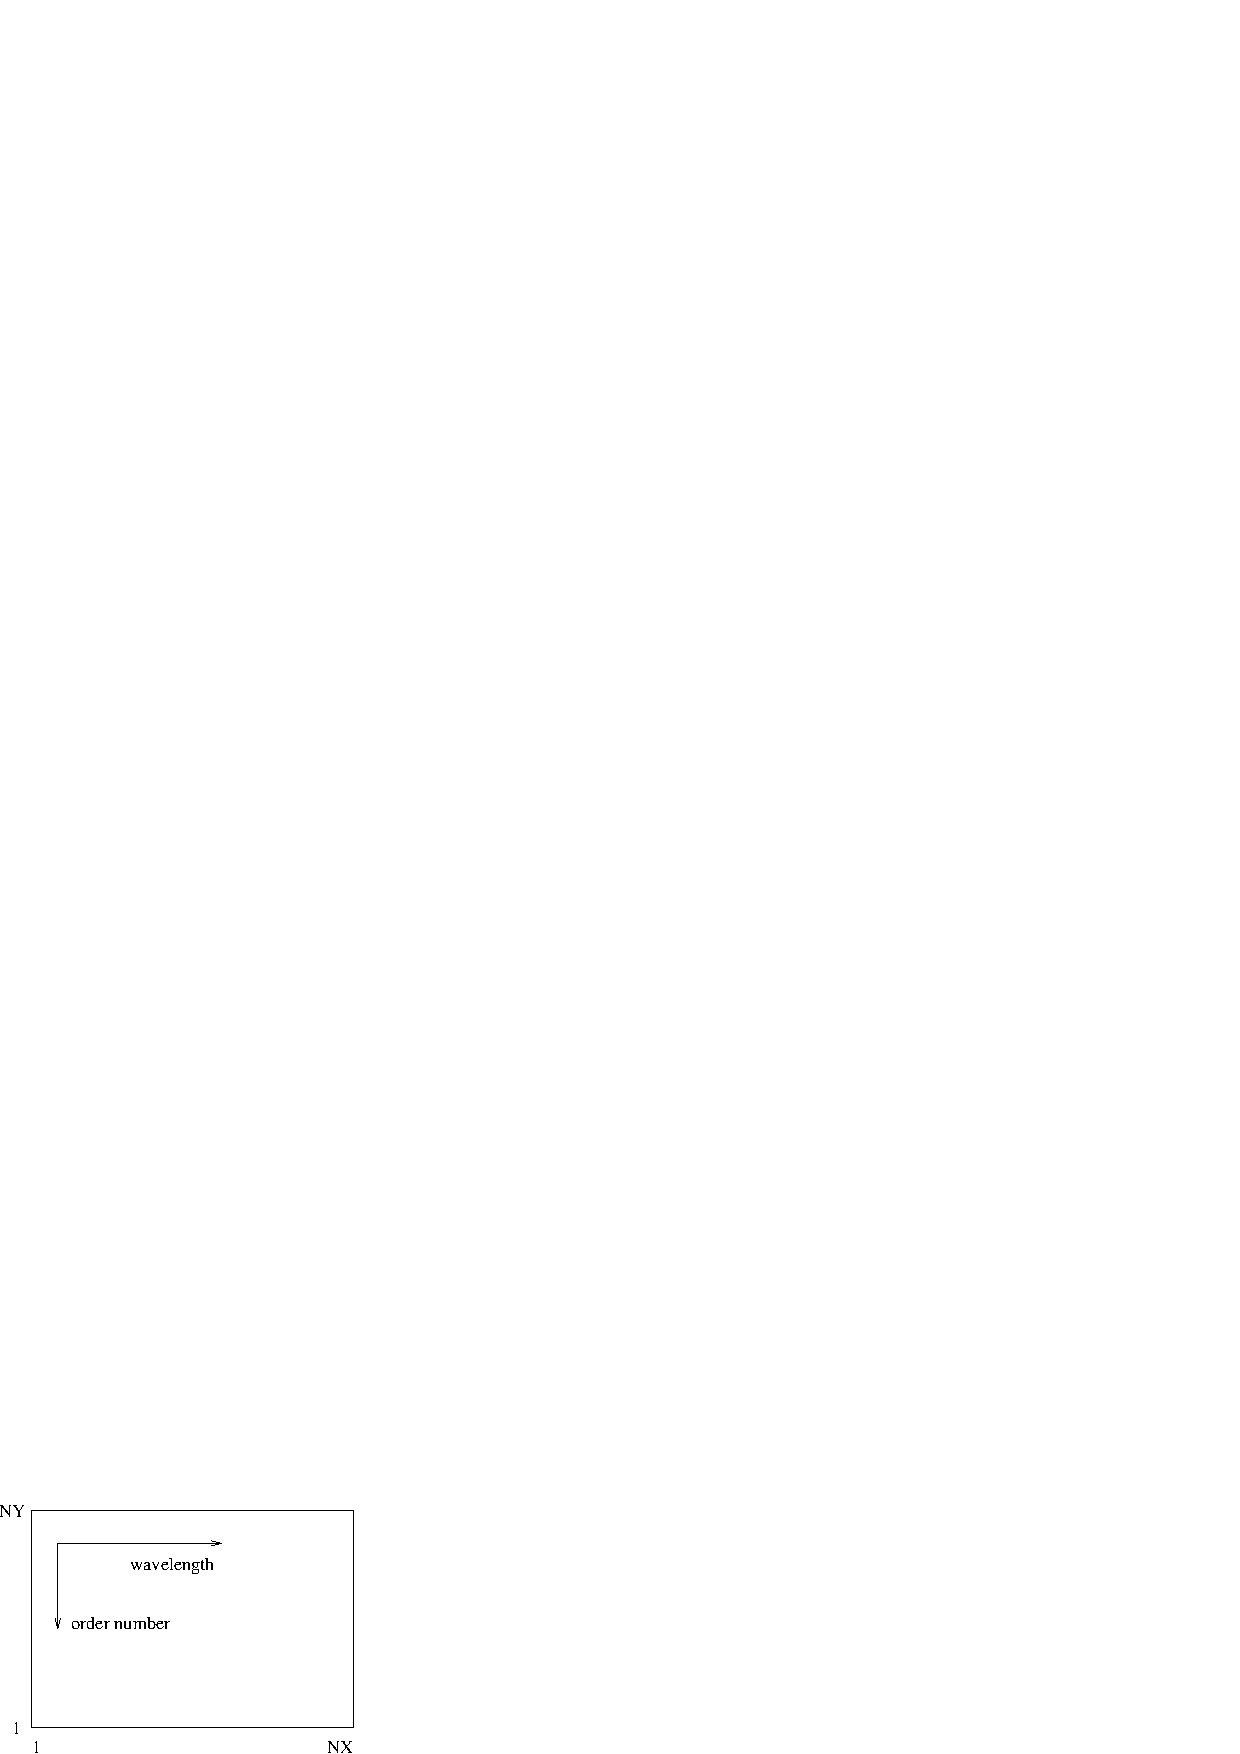
\includegraphics{sun86_ech5}
\caption{Conventional orientation for \'echelle reduction.}
\end{center}
\end{figure}

   The first thing to do is to ensure that your data is in the
   conventional orientation with wavelength increasing from left to
   right and from bottom to top of the image and thus with order number
   decreasing from bottom to top of the image.

   IPCS data will already be in this orientation but unfortunately CCD
   data must be rotated and flipped. This is quite time-consuming but is
   at present necessary for all CCD images. The following commands
   achieve this for the continuum:

\begin{terminalv}
ICL> irot90 contraw contrawrot
ICL> irevy  contrawrot cont
\end{terminalv}

   with analogous commands for the arc and the object. The \emph{raw\/}
   files can now be deleted if desired.

   In what follows, assume that the IPCS raw data files `contraw.sdf' have
   been renamed to `cont.sdf' etc.

\begin{figure}[htb]
\begin{center}
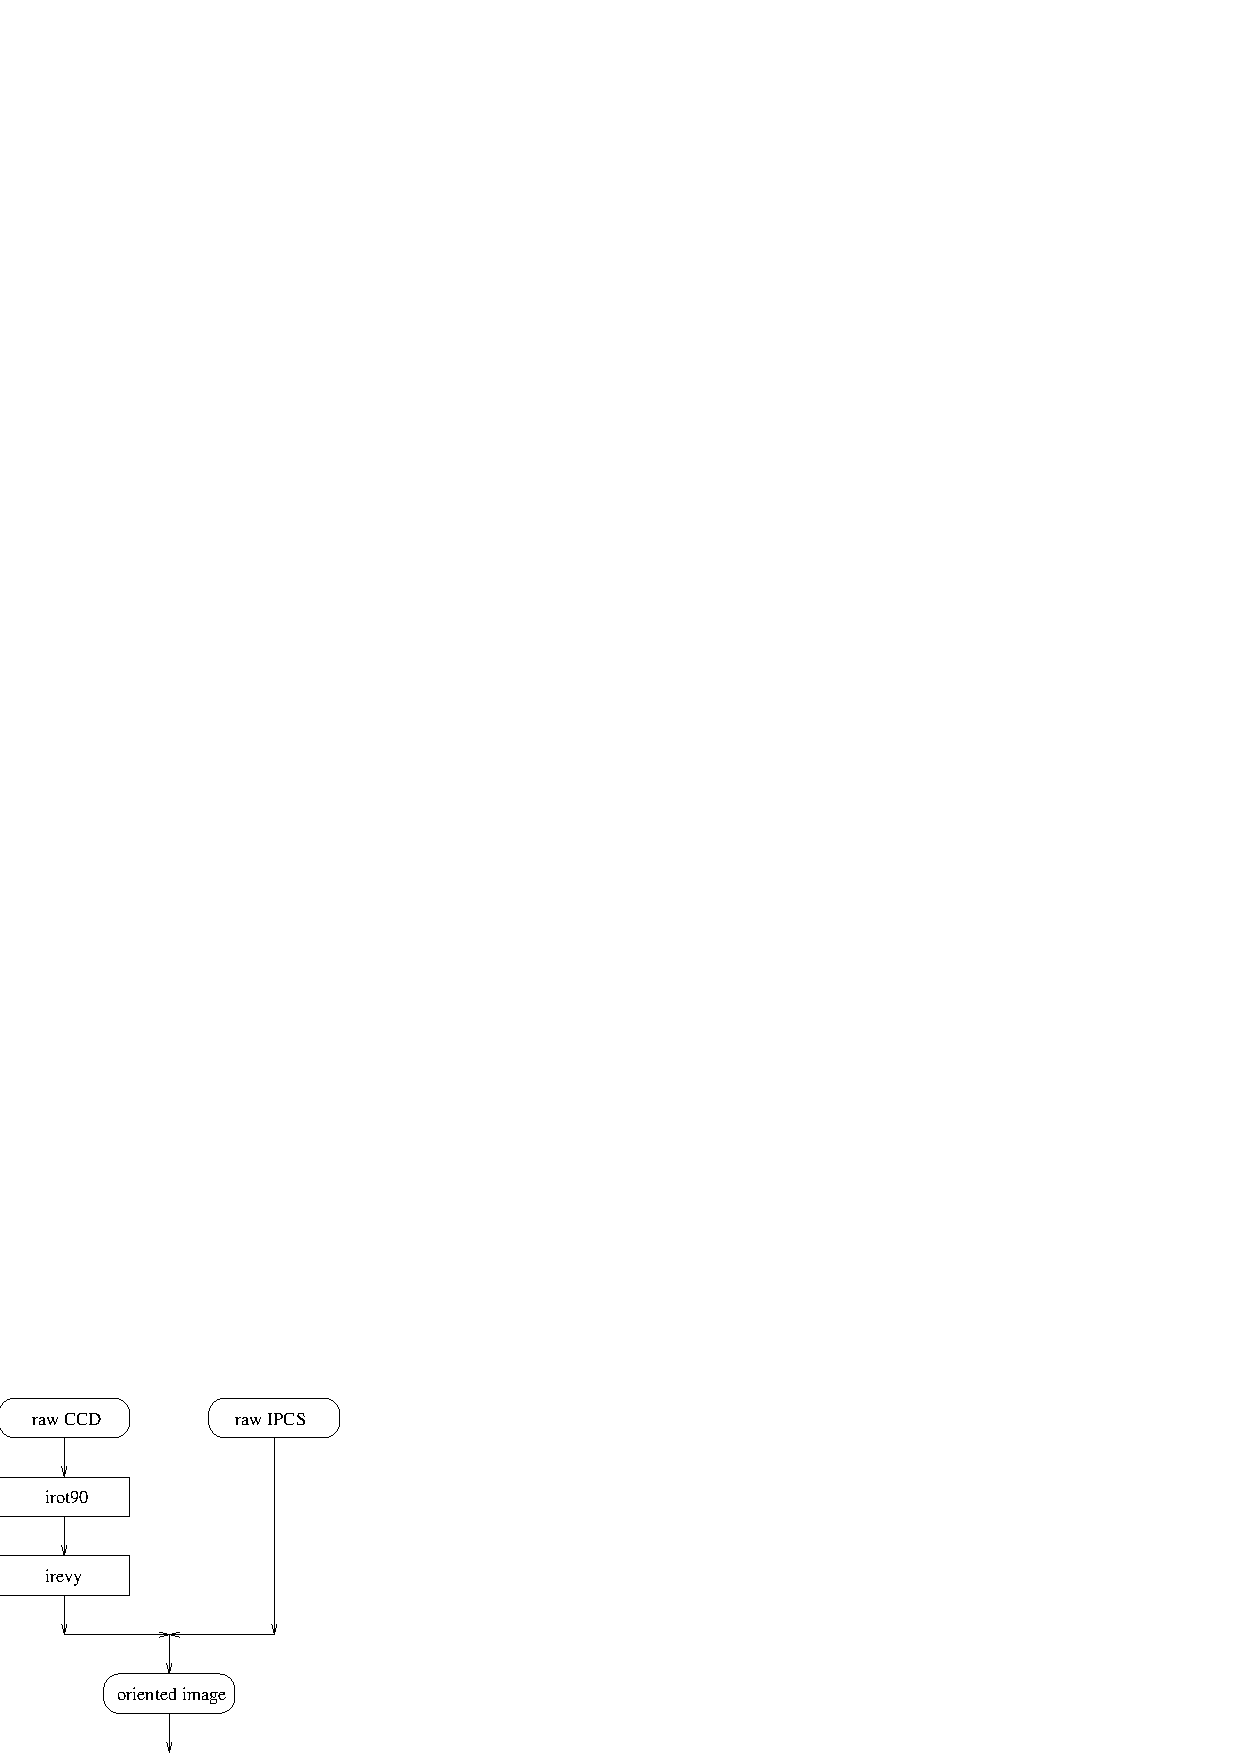
\includegraphics{sun86_ech1}
\caption{Flow chart for reorienting CCD.}
\end{center}
\end{figure}

%       -----------------------------------------------------------------------

\subsubsection{\label{techno13locate}Order location}

\begin{figure}[htb]
\begin{center}
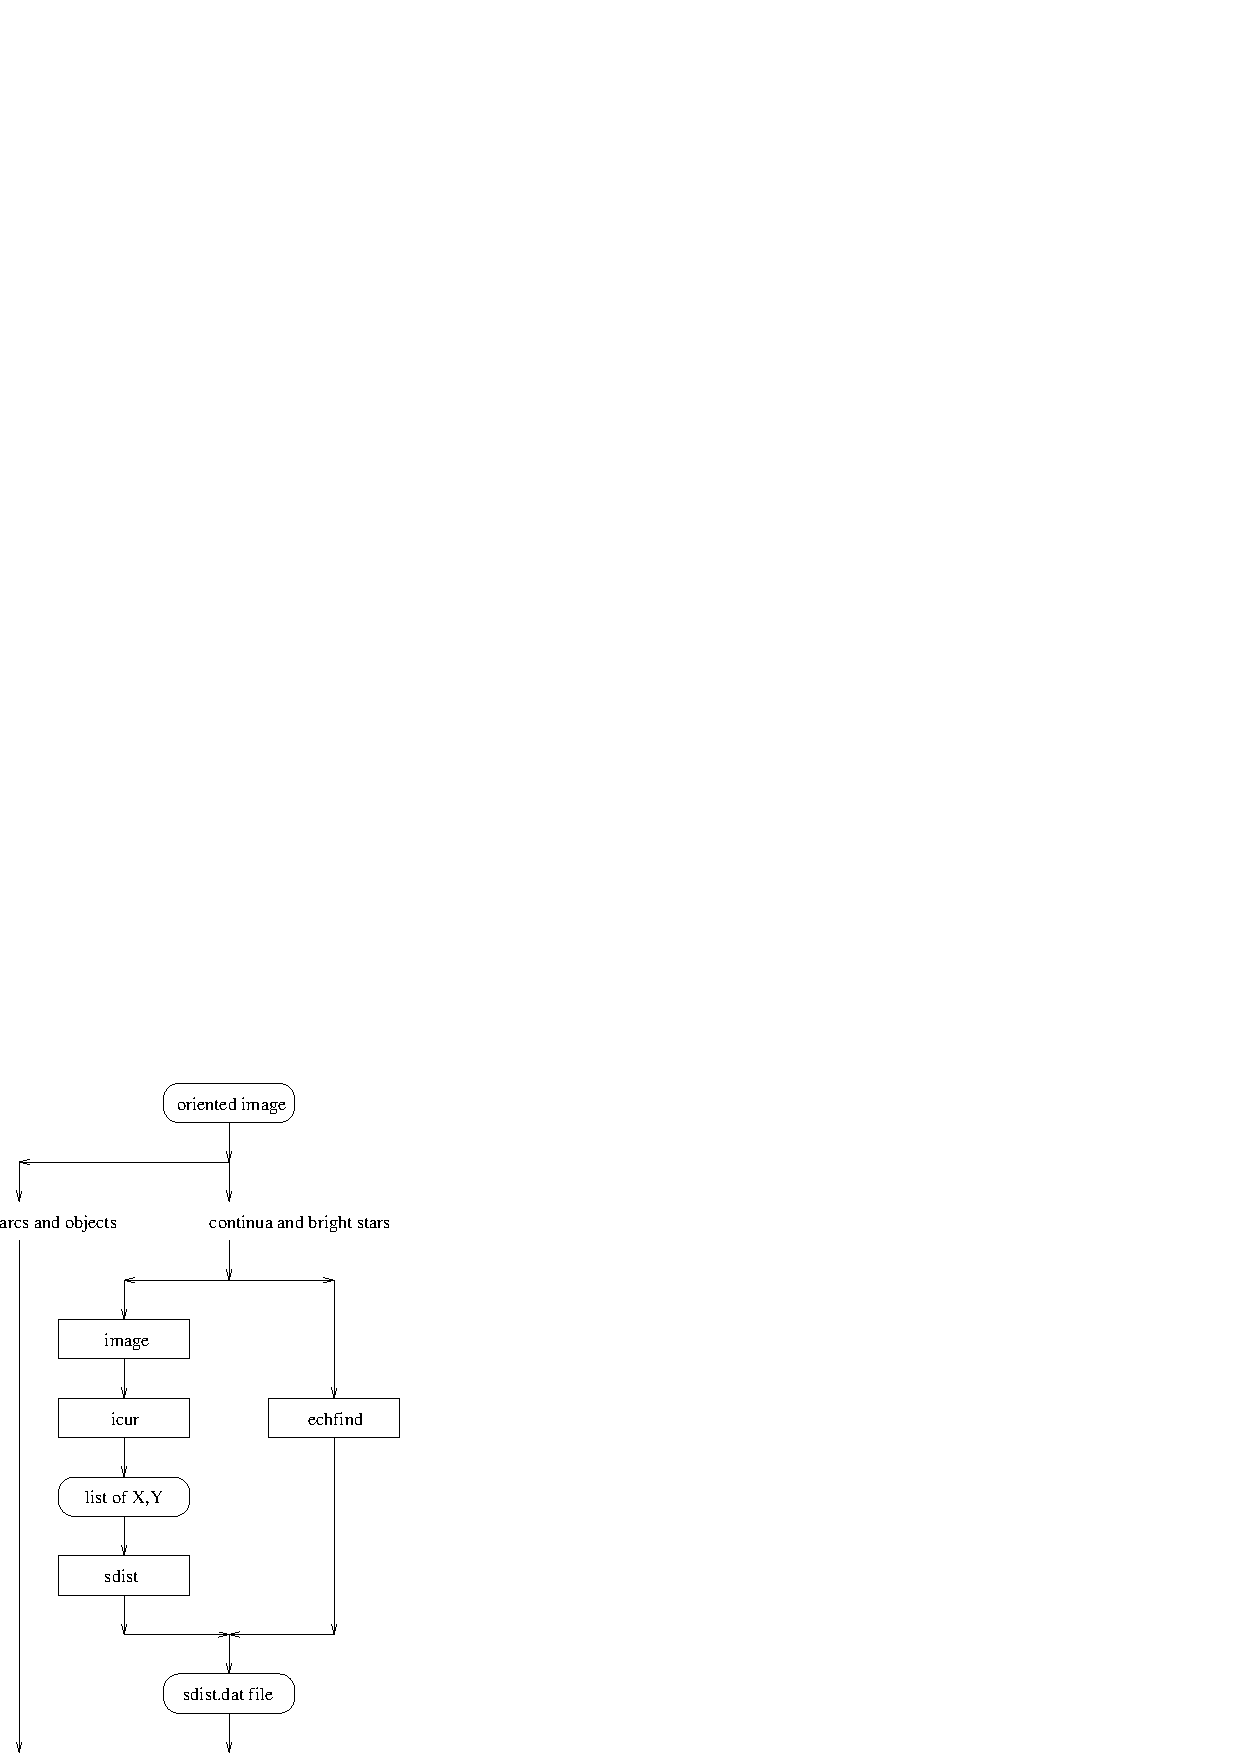
\includegraphics{sun86_ech2}
\caption{Flow chart for locating \'echelle orders.}
\end{center}
\end{figure}

   At present locating the orders is rather an interactive process
   (there is a program `echfind' that does it automatically but it does
   not yet work very well in all cases and its use is not recommended).

   First decide whether you are going to use the continuum source or the
   object to locate the orders. It is a good idea first to do a
   `ystract' / `splot' of the data to get a feel for the width,
   intensity and profiles of the orders. Sensible commands to use for
   the GEC chip and the continuum are:

\begin{terminalv}
ICL> ystract cont 185 194 s
ICL> splot s reset accept
\end{terminalv}

   Now display the image using `image':

\begin{terminalv}
ICL> image cont high=hhhh reset accept
\end{terminalv}

   The next stage is to use `icur' to define a point somewhere near the
   peak of each order that you wish to track and extract. You can track
   orders that are only partially on the image if you wish to but this
   is not recommended, since it could well affect the wavelength
   calibration, especially if only a small part of the free spectral
   range is being covered. It is quite important to choose points close
   to the peak intensity.

\begin{terminalv}
ICL> icur
\end{terminalv}

   Now run `sdist' to track the orders and fit polynomials to them:

\begin{terminalv}
ICL> sdist image=cont columns=8 trace=G width=3 maxdeg=10 softd=no
\end{terminalv}

   The two non-obvious parameters are `trace' and `width'. Specify
   `Gaussian' for `trace' if the profiles across the orders are roughly
   Gaussian and are not cut off by the dekker. Normally specify `COG'
   otherwise but if there is a noticeable gradient along the profile you
   can try `Edge' (they are identical in that both locate the rising and
   falling edges of the orders, but `COG' estimates the centre by
   calculating the centre of gravity and `Edge' estimates it simply by
   taking the mean of the edge positions). For `width', specify an
   estimate of the FWHM for `Gaussian' and an estimate of half the order
   width for `COG' and `Edge'. If anything, underestimate it for
   `Gaussian' and overestimate it for `COG' and `Edge'.

   Beware that sky data can confuse `sdist' because it gives rise to
   profiles that don't fit any of the trace modes. If this appears to be
   a problem, use `clip' (which sets all data values below a given low
   value to that low value and sets all values above a given high value
   to that high value) to get rid of the sky data values that are
   causing the problem.

   There is another program that may be useful here if you have moved
   to a new object that is not quite in the same place on the slit.
   `offdist' operates on an `sdist.dat' file and adjusts the constant
   terms so as to shift the tracked orders up or down by a specified
   amount.

%       -----------------------------------------------------------------------

\subsubsection{\label{techno13extract}Order extraction}

\begin{figure}[htb]
\begin{center}
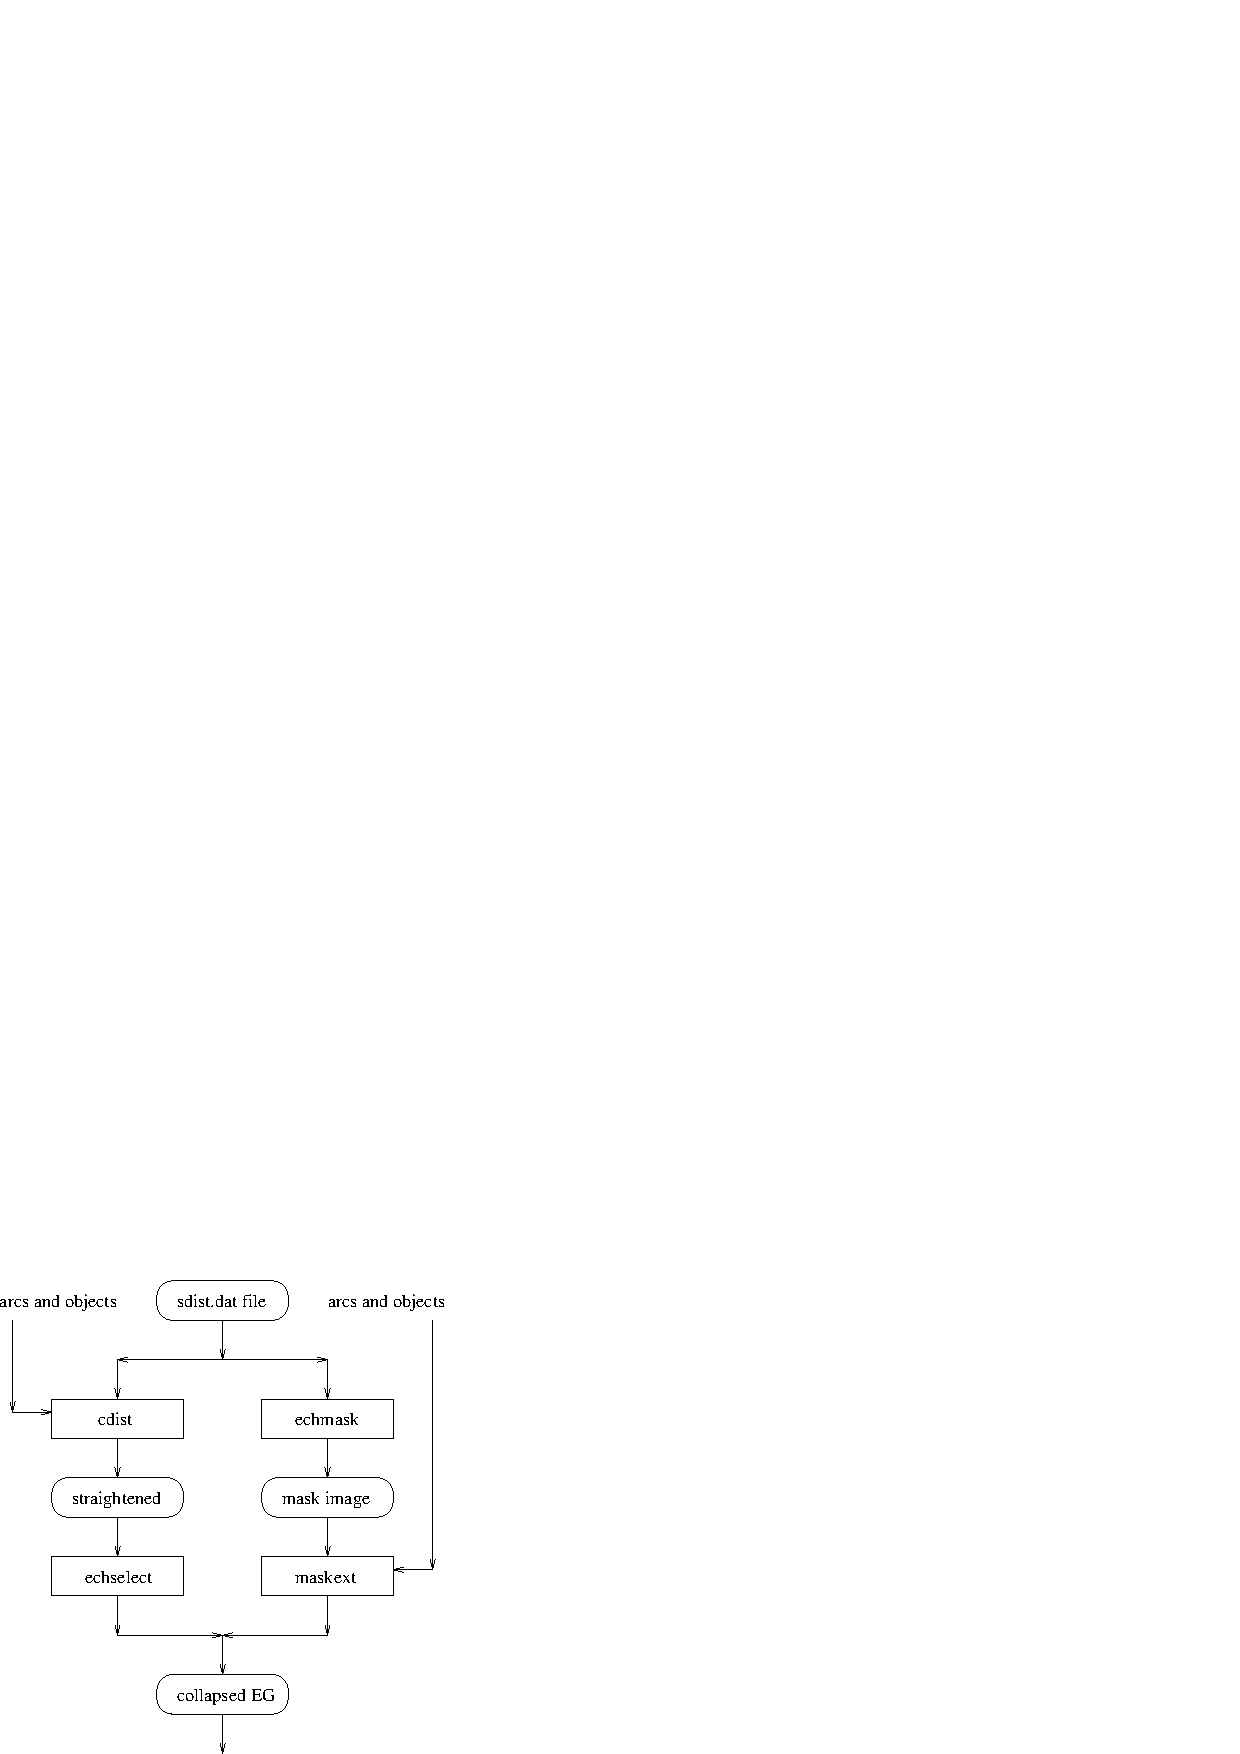
\includegraphics{sun86_ech3}
\caption{Flow chart for extracting orders in \'echelle spectra.}
\end{center}
\end{figure}

   You now have a choice. For quick-look extraction, you can create a
   mask image whose data values indicate which order (if any) each pixel
   belongs to. This mask is created by `echmask' and applied by
   `maskext'. `echmask' allows separate extraction of object and sky but
   requires the number of rows of object and sky data to be independent
   of order number. This is not acceptable when (as is usually the case)
   it is important to minimise the sky noise and to maximise the signal.

   For final data reduction or where the use of a mask is not acceptable
   the orders can be straightened using `cdist' (UCLES is extremely
   stable and preliminary results indicate that many images can be
   co-added prior to application of `cdist', so the cost in processing
   time should be acceptable). Having straightened the orders,
   `echselect' can be run to identify, for each order, the rows to be
   used for the object and those to be used for sky.

   The result in both cases is a `collapsed \'echellogram' where X is
   wavelength and Y is order number. Your object image will of course
   give rise to both an object and a sky \'echellogram.

%       -----------------------------------------------------------------------

\subsubsection{Quick-look extraction using a mask}

   As explained above, this method will not maximise signal to noise
   ratio, but it will do a reasonably good job, especially where the
   orders in question are not too far from being horizontally aligned on
   the detector.

%       -----------------------------------------------------------------------

\subsubsection{Mask creation}

   `sdist' outputs an `sdist.dat' file that contains details of the
   orders that it has tracked. This file is read by `echmask', which
   produces a mask image that can be used for fast extraction of orders
   directly from (in the case of the CCD `irot90-ed' and `irevy-d') raw
   images.  `echmask' can cope with the case where the star / sky
   periscope is fitted and also allows you to specify the position of
   object and sky data relative to the centre of the order as determined
   by the tracking algorithm, but these details will be ignored here.

   The normal straightforward behaviour is achieved by specifying
   `periscope' false and giving zeroes for all widths and offsets. This
   causes a width derived from the `sdist' fit to be used; if the fit
   was Gaussian the derived width is just twice the estimate that you
   gave to `sdist' and if the fit was Edges it is the actual calculated
   width (the same width is used for each order and the third largest
   width of all the order widths is used so as to exclude atypical
   values). If you know better, you can specify your own value for
   `objwidth'\latorhtm{---}{-}overestimate rather than underestimate so as
   to prevent
   noticeable jumps in the extracted data due to the slope and curvature
   of the orders.

   The other thing that `echmask' needs to know is the order numbers
   corresponding to the orders that it has tracked. The value that you
   give for `mstart' is the order number corresponding to the first
   point that you selected with `icur'. There should always be an order
   near to the image centre. Don't worry if you get it
   wrong\latorhtm{---}{-}you can
   always adjust the order number by using `icadd' to add or subtract
   the error from the mask structure. You have to add or subtract ten
   counts to adjust by one order, e.g.\ if the mask contains a data value
   of 420, this refers to order 42 and adding ten to it to make it 430
   causes it to refer to order 43.

   This is a typical run of `echmask'.

\begin{terminalv}
ICL> echmask cofile=sdist.dat periscope=no objwidth=0 objoffset=0 ~
    s1width=10 s1offset=9 s2width=0 mstart=82 ~
    mdelta=-1 mask=mask
*** Will use an OBJWIDTH of  6 pixels
\end{terminalv}

   When running with the periscope, each order is split up into two
   parts, each of which looks rather like an order in its own right. If
   you are unsure how they are grouped, display an arc and all will be
   revealed. When using the periscope it is your responsibility to
   ensure that the first and second points selected with `icur'
   correspond to the two parts of the same order and similarly for the
   third and fourth points etc.

%       -----------------------------------------------------------------------

\subsubsection{Mask extraction}

   The resulting mask image can be used for fast extraction of orders
   from (in the case of the CCD `irot90-ed' and `irevy-d') raw images
   taken at the same spectrograph configuration as it. This is done
   using the `maskext' program. `maskext' needs to be told the range
   of order numbers that you want to extract and this determines the Y
   size of the extracted file (referred to as a collapsed \'echellogram)
   and its Y units.

   The `sub-order' controls which bits of the order are extracted into
   the output image. A sub-order of 0 always extracts object and sky and
   sub-orders of 1 and 2 can be used to extract object and sky
   separately. If the periscope is fitted, sub-order 2 corresponds to
   the first encountered part of the order and sub-order 1 corresponds
   to the second encountered part of the order (so if the tracked orders
   went from the bottom upwards the data values in the mask are
   monotonically decreasing as you go from bottom to top). If the
   periscope is not fitted, sub-order 1 always refers to object and
   sub-order 2 always refers to sky. This is confusing and will probably
   change!

\begin{terminalv}
ICL> maskext image=arc mask=mask mlow=68 mhigh=82 subord=0 output=arce
\end{terminalv}

%       -----------------------------------------------------------------------

\subsubsection{\label{techno13accurate}
   Accurate extraction from straightened orders}

   The trouble with curved orders is that when the object projects to
   only one or two pixels on the detector, the bulk of the signal will
   sometimes fall into one pixel and sometimes it will be split between
   several pixels. This means that there is no single correct number of
   rows of data to extract, forcing the extraction of unwanted sky as
   well as wanted signal.

   Obviously it would be possible to provide a program that would make
   a sensible decision about how many rows of data to extract at each
   point along the order, and we intend investigating the use of some
   optimal weighted extraction scheme. However, any such scheme needs
   accurate knowledge of the noise characteristics of the data and it
   would take considerable effort to implement a reliable automatic
   extraction algorithm.

   Accordingly, the recommended approach for accurate extraction is
   first to use the `cdist' program to re-sample in the Y direction so
   as to straighten the orders. Experience shows that this program
   does an excellent job, with little discernible loss of resolution or
   variation of profile along the order. Once the orders are
   straightened, the number of rows to extract for object and for sky is
   merely a function of order number and not of wavelength.

%       -----------------------------------------------------------------------

\subsubsection{Order straightening}

   The `cdist' program uses the `sdist.dat' file that was written by
   `sdist'. It uses the polynomial coefficients to re-sample in Y so as
   to straighten the corresponding orders.

\begin{terminalv}
ICL> cdist image=arc ystart=1 yend=250 output=arcc maxdegy=5
\end{terminalv}

%       -----------------------------------------------------------------------

\subsubsection{Order extraction}

   Having got an image with straight orders, conceptually one wants to
   take a `ystract' through somewhere near the centre of the orders,
   display with `splot' and then, for each order, somehow identify which
   rows are to be used for object and for sky. Having done this, the
   relevant rows can be extracted into a collapsed \'echellogram of the
   same format as that produced by `maskext'.

   `echselect' allows the user to indicate interactively the
   cross-sections of a corrected \'echellogram to be used as object and
   sky for the various orders. It then creates a collapsed \'echellogram
   for the object orders, and\latorhtm{---}{-}optionally\latorhtm{---}{-}one
   for the sky orders.

%       -----------------------------------------------------------------------

\subsubsection{\label{techno13calib}Wavelength calibration}

\begin{figure}[htb]
\begin{center}
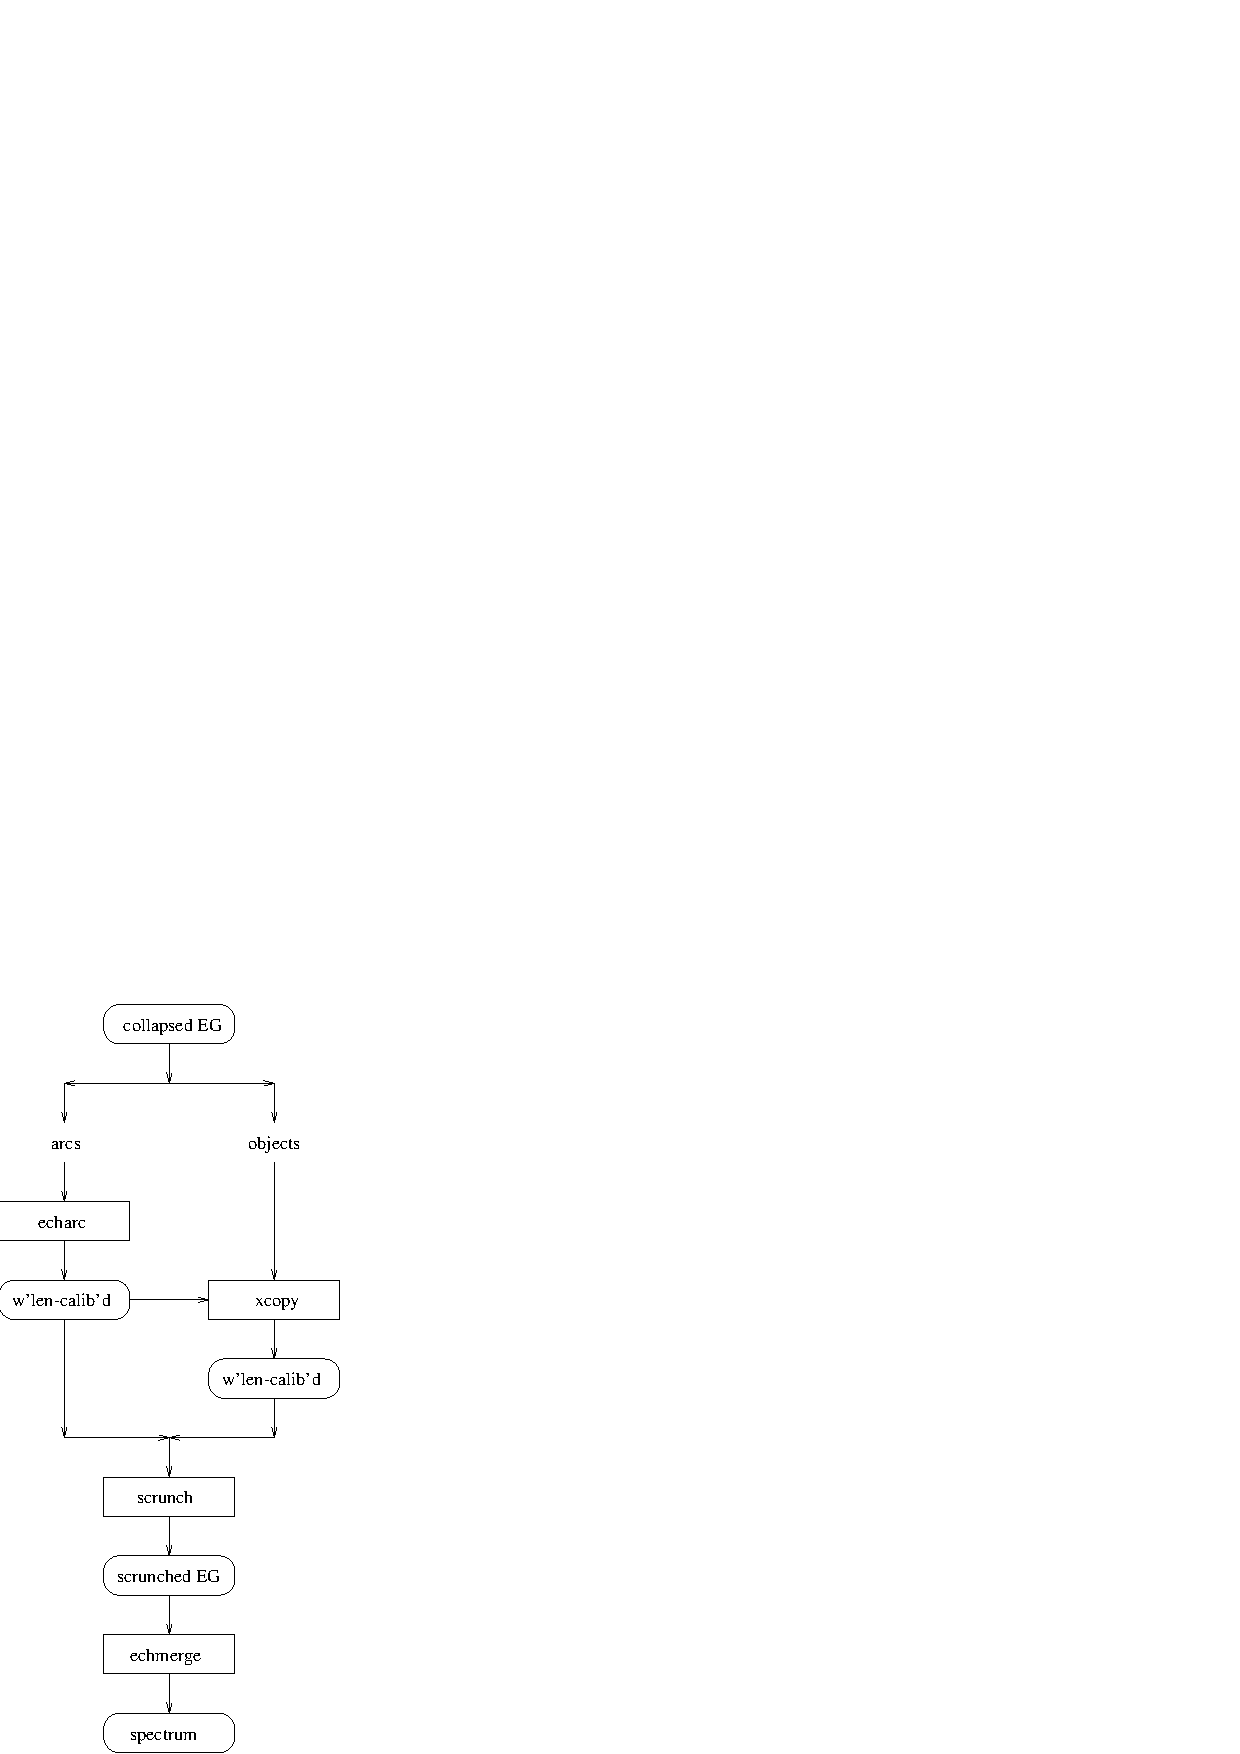
\includegraphics{sun86_ech4}
\caption{Wavelength calibrating an \'echelle spectrum.}
\end{center}
\end{figure}

   We are now at the stage where arc and object have both had their
   orders extracted into collapsed \'echellograms. These are
   two-dimensional images with X still being pixel number and Y being
   order number. The `echarc' program is used for identifying lines in
   the arc. This writes wavelength calibration data as a two-dimensional
   arce.\-AXIS(1).\-MORE.\-FIGARO.\-DATA\_\-ARRAY.\-DATA array and the
   arce.AXIS(1) structure is then copied to the obje.AXIS(1) structure
   using the `xcopy' program.

   `echarc' works by first of all doing the equivalent of the
   one-dimensional `arc' program on a set of three or more orders that
   you nominate to be fitted interactively. Then it enters an automatic
   mode where lines are identified in all the other orders. It estimates
   wavelength in the other orders by fitting lines of constant
   (order number)*(wavelength) between the interactively fitted orders.

   Experience with `echarc' has shown that it is vital to include the
   extreme orders among those that are interactively fitted, that it may
   well be worth using four rather than three interactively fitted
   orders, that a good line list is absolutely vital and that if things
   start going wrong then they will probably stay wrong (use of Ctrl-C
   is recommended in this case). Care with the interactively fitted
   orders is usually rewarded.

   The file `arlines.ech' always contains details of identified lines
   and if a fit fails a good policy is to restart using the results from
   the previous fit and perhaps selecting slightly different
   interactively fitted orders, e.g.\ add the orders that were worst in
   the automatic phase from the previous run. All the lines previously
   identified in the orders that are to be interactively fitted are
   still available so a re-run is not too time-consuming.

   Also note that it is necessary to rename any old files of name
   `arlines.ech' before running `echarc'.

   The `dowaves' keyword should always be false (if it is true then the
   wavelength information is written to a separate file and we want it
   in the input file for the purpose of scrunching). Also note that if
   the `monitor' keyword is true then a graphical record of how the
   automatic mode is proceeding will be output to the soft device.

   Here is a typical example of `echarc'.

\begin{terminalv}
ICL> echarc image=arce arctype=thar previous=no interactive=3 ~
    orders=[82,75,68] orderfit=5 sigma=3 dowaves=no
\end{terminalv}

   After a successful arc fit, use `xcopy' to copy the `arce.AXIS(1)'
   structure to the `obje.AXIS(1)' structure.

\begin{terminalv}
ICL> xcopy spectrum=obje arc=arce output=obje
\end{terminalv}

%       -----------------------------------------------------------------------

\subsubsection{\label{techno13scrunch}Scrunching}

   The next step is to scrunch the wavelength calibrated `obje' and
   `arce' files. Contrary to possible expectation the program used is
   `scrunch' rather than `iscrunch'. Rather than using an `arlines.iar'
   file, `scrunch' uses the two-dimensional
   .AXIS(1).\-MORE.\-FIGARO.\-DATA\_\-ARRAY.\-DATA array produced by
   `echarc' as its source of wavelength information. You tell it the
   wavelength range and the number of bins that you want to scrunch into
   and whether to use a linear or logarithmic wavelength scale and it
   does the rest.

   Since the \'echelle spectra are such that a pixel corresponds to
   a fixed velocity interval irrespective of wavelength (e.g., 22
   microns = 2.73 km/s), a logarithmic wavelength scale will give bins
   that each correspond to the same number of pixels, whereas a linear
   wavelength scale will give bins at the red end that significantly
   oversample the resolution element relative to bins at the blue end.
   However, a linear scrunch will still probably be the favoured option
   in many cases.

   It's probably worth using `hdstrace' to look at the file to find
   out the minimum and maximum wavelengths before running `scrunch'.

\begin{terminalv}
ICL> scrunch spectrum=obje log=no wstart=4000 wend=0.02 bins=5000 ~
    mean=no quad=yes output=objs
\end{terminalv}

   Every order will be scrunched into the full wavelength range (4550 to
   5000 Angstroms in the above example) and consequently most pixels
   will be zero.

%       -----------------------------------------------------------------------

\subsubsection{\label{techno13merge}Merging orders}

   The final stage is to merge the scrunched orders from possibly
   several images into a single long spectrum. This is done using the
   `echmerge' program. If the data is from a region of the field where
   the full free spectral range is obtained then adjacent orders will
   overlap and the contributions from the overlapping orders are
   weighted with estimates of their inverse variances on the assumption
   of purely Poisson noise. Where one contribution is below a given
   fraction of the other then it is ignored completely. The variance
   estimates are based on median filtered versions of the input orders
   and the median filter box size is controlled by the `box' parameter.

   The input images must all have the same X size, units and values and
   can be one-dimensional or two-dimensional. The output image is always
   one-dimensional and can be the same as either of the input files, in
   which case no new image is created. The second input image can be
   specified as blank in which case it is not required or used.

\begin{terminalv}
ICL> echmerge image=objs image1='' box=7 cutoff=4 output=objl
\end{terminalv}

%       -----------------------------------------------------------------------

\subsubsection{\label{techno13summary}Summary of the example}

   Here there is just a reference list of the programs that were run
   above.

\begin{terminalv}
 { conventional orientation (CCD)
   ICL> irot90 contraw contrawrot
   ICL> irevy  contrawrot cont
   ICL> irot90 arcraw arcrawrot
   ICL> irevy  arcrawrot arc
   ICL> irot90 objraw objrawrot
   ICL> irevy  objrawrot obj

 { review of counts, widths and shapes
   ICL> ystract cont 185 194 s
   ICL> splot s reset accept
   ICL> image cont high=hhhh reset accept

 { select points on orders
 { track and fit orders
   ICL> icur
   ICL> sdist cont .

 { Either ...

    { create mask
      ICL> echmask sdist.dat . mask
    { extract orders using mask
      ICL> maskext arc mask . arce
      ICL> maskext obj mask . obje

 { Or ...

    { straighten orders
      ICL> cdist arc . arcc
      ICL> cdist obj . objc
    { extract orders
      ICL> echselect arcc arce
      ICL> echselect objc obje

 { End either.

 { identify arc lines
   ICL> echarc arce .
 { copy wavelength info to object
   ICL> xcopy obje arce obje

 { scrunch arc and object
   ICL> scrunch arce . arcs
   ICL> scrunch obje . objs

 { merge orders
   ICL> echmerge arcs . arcl
   ICL> echmerge objs . objl
\end{terminalv}

% =============================================================================

\appendix\newpage
\addcontentsline{toc}{part}{Appendices}

% -----------------------------------------------------------------------------

\section{\xlabel{commands_classified}\label{classif}Classified list of commands}


%       -----------------------------------------------------------------------

\subsection{\label{classifinput}Data input}

\htmlref{ALASIN}{ALASIN} --- Read a spectrum in ALAS (Abs. Line Analysis System) format\\
\htmlref{FITSET}{FITSET} --- Set the value of a FITS keyword\\
\htmlref{FITSKEYS}{FITSKEYS} --- List the FITS keywords in a data file\\
\htmlref{ICOR16}{ICOR16} --- Corrects 16 bit data from signed to unsigned range\\
\htmlref{RCGS2}{RCGS2} --- Reads UKIRT CGS2 spectrum (also UKT9 and UKT6 CVF)\\
\htmlref{RDFITS}{RDFITS} --- Read file in AAO de facto `Disk FITS' format\\
\htmlref{RDIPSO}{RDIPSO} --- Read file in DIPSO/IUEDR/SPECTRUM format\\
\htmlref{TABLE}{TABLE} --- List contents of a SPICA memory file

%       -----------------------------------------------------------------------

\subsection{\label{classifoutput}Data output}

\htmlref{ALASOUT}{ALASOUT} --- Output a spectrum in ALAS (Abs. Line Analysis System) format\\
\htmlref{WDFITS}{WDFITS} --- Writes an image out in the AAO de facto 'Disk FITS' format\\
\htmlref{WDIPSO}{WDIPSO} --- Writes a file in DIPSO/IUEDR/SPECTRUM format

%       -----------------------------------------------------------------------

\subsection{\label{classifdisplay}Display commands}

\htmlref{CCUR}{CCUR} --- After SPLOT, uses graphics cursor to indicate data values\\
\htmlref{COLOUR}{COLOUR} --- Set colour table for image display\\
\htmlref{DVDPLOT}{DVDPLOT} --- Plot the data in one file against the data in another\\
\htmlref{ELSPLOT}{ELSPLOT} --- Produces a long ($<$3m) error bar plot of a spectrum\\
\htmlref{ESPLOT}{ESPLOT} --- Produces an error bar plot of a spectrum\\
\htmlref{HARD}{HARD} --- Sets the file name for hard copy output\\
\htmlref{HOPT}{HOPT} --- Histogram optimisation of an image\\
\htmlref{ICONT}{ICONT} --- Produces a contour map of an image\\
\htmlref{ICUR}{ICUR} --- Inspect an image with cursor\\
\htmlref{IDEV}{IDEV} --- Set the device for image display\\
\htmlref{IGCUR}{IGCUR} --- Use cursor to show x, y and data values\\
\htmlref{IGREY}{IGREY} --- Produces a grey-scale plot of an image\\
\htmlref{IMAGE}{IMAGE} --- Display an image on the selected image display\\
\htmlref{IPLOTS}{IPLOTS} --- Plots successive cross-sections of an image, several to a page\\
\htmlref{ISPLOT}{ISPLOT} --- Plots successive cross-sections through an image\\
\htmlref{LSPLOT}{LSPLOT} --- Hardcopy spectrum plot of specified size (up to 3 metres)\\
\htmlref{MSPLOT}{MSPLOT} --- Plots a long spectrum as a series of separate plots\\
\htmlref{SOFT}{SOFT} --- Sets the device/type for terminal graphics\\
\htmlref{SPLOT}{SPLOT} --- Plots a spectrum\\
\htmlref{XCUR}{XCUR} --- Uses cursor to delimit part of a spectrum

%       -----------------------------------------------------------------------

\subsection{\label{classifwavelen}Wavelength calibration}

\htmlref{ARC}{ARC} --- Interactive manual arc line identification\\
\htmlref{ECHARC}{ECHARC} --- Fit an \'echelle arc\\
\htmlref{EMLT}{EMLT} --- Fits gaussians to the strongest lines in a spectrum\\
\htmlref{FSCRUNCH}{FSCRUNCH} --- Rebin data with a disjoint wavelength coverage to a linear one\\
\htmlref{IARC}{IARC} --- Given fit to single spectrum, fit all spectra in a 2-D arc\\
\htmlref{ISCRUNCH}{ISCRUNCH} --- Rebin an image to linear wavelength scale given IARC results\\
\htmlref{ISCRUNI}{ISCRUNI} --- Like ISCRUNCH, but interpolates between two IARC result sets\\
\htmlref{LXSET}{LXSET} --- Set X array of spectrum/image to specified range\\
\htmlref{SCRUNCH}{SCRUNCH} --- Rebin a spectrum to a linear wavelength range\\
\htmlref{VACHEL}{VACHEL} --- Air to vacuum, and/or recession velocity wavelength conversion\\
\htmlref{XCOPI}{XCOPI} --- Like XCOPY but interpolates X-data from 2 files\\
\htmlref{XCOPY}{XCOPY} --- Copy X-info (eg wavelengths) into a spectrum

%       -----------------------------------------------------------------------

\subsection{\label{classifbstars}B-star calibration}

\htmlref{BSMULT}{BSMULT} --- Atmospheric band removal using a B-star calibration spectrum\\
\htmlref{CFIT}{CFIT} --- Generate a spectrum using the cursor\\
\htmlref{CSET}{CSET} --- Interactively set regions of a spectrum to a constant value\\
\htmlref{MASK}{MASK} --- Generate a mask spectrum given a spectrum and a mask table\\
\htmlref{MCFIT}{MCFIT} --- Fit a continuum to a spectrum, given a mask spectrum\\
\htmlref{NCSET}{NCSET} --- Set a region of a spectrum to a constant

%       -----------------------------------------------------------------------

\subsection{\label{classifarith}Arithmetic operations}

\htmlref{CLIP}{CLIP} --- Clip data above and below a pair of threshold values\\
\htmlref{IADD}{IADD} --- Adds two images (or two spectra)\\
\htmlref{IALOG}{IALOG} --- Takes the antilog of an image\\
\htmlref{ICADD}{ICADD} --- Adds a constant to an image\\
\htmlref{ICDIV}{ICDIV} --- Divides an image by a constant\\
\htmlref{ICMULT}{ICMULT} --- Multiplies an image by a constant\\
\htmlref{ICONV3}{ICONV3} --- Convolve an image with a 3x3 convolution kernel\\
\htmlref{ICSUB}{ICSUB} --- Subtracts a constant from an image\\
\htmlref{IDIFF}{IDIFF} --- Takes the 'differential' of an image\\
\htmlref{IDIV}{IDIV} --- Divides two images (or two spectra)\\
\htmlref{IGCONV}{IGCONV} --- Convolve an image with a specified filter\\
\htmlref{ILOG}{ILOG} --- Takes the logarithm of an image\\
\htmlref{IMULT}{IMULT} --- Multiplies two images (or two spectra)\\
\htmlref{IPOWER}{IPOWER} --- Raises an image to a specified power\\
\htmlref{IREVX}{IREVX} --- Reverse an image (or spectrum) in the X-direction\\
\htmlref{IREVY}{IREVY} --- Reverse an image in the Y-direction\\
\htmlref{ISHIFT}{ISHIFT} --- Applies a linear x and a linear y shift to an image\\
\htmlref{ISMOOTH}{ISMOOTH} --- 2-D smooth of image using 9-point smoothing algorithm\\
\htmlref{ISTRETCH}{ISTRETCH} --- Stretches and shifts an image in X and Y.\\
\htmlref{ISUB}{ISUB} --- Subtracts two images (or two spectra)\\
\htmlref{ISUBSET}{ISUBSET} --- Produces a subset of an image\\
\htmlref{ISUPER}{ISUPER} --- Produces a superset of an image\\
\htmlref{ISXADD}{ISXADD} --- Adds a spectrum to each X direction x-section of an image\\
\htmlref{ISXDIV}{ISXDIV} --- Divides a spectrum into each X direction x-section of an image\\
\htmlref{ISXMUL}{ISXMUL} --- Multiplies each X direction image x-sect by a spectrum\\
\htmlref{ISXSUB}{ISXSUB} --- Subtracts a spectrum from each X direction x-section of an image\\
\htmlref{ISYADD}{ISYADD} --- Adds a spectrum to each Y direction x-section of an image\\
\htmlref{ISYDIV}{ISYDIV} --- Divides a spectrum into each Y direction x-section of an image\\
\htmlref{ISYMUL}{ISYMUL} --- Multiplies each Y direction image x-sect by a spectrum\\
\htmlref{ISYSUB}{ISYSUB} --- Subtracts a spectrum from each Y direction x-section of an image\\
\htmlref{IXSMOOTH}{IXSMOOTH} --- Smooth in x-direction by gaussian convolution\\
\htmlref{RESAMPLE}{RESAMPLE} --- Rebin an image to different dimensions and/or orientation\\
\htmlref{RESCALE}{RESCALE} --- Rescale using user-defined upper and lower limits\\
\htmlref{ROTX}{ROTX} --- Rotate data along the X-axis

%       -----------------------------------------------------------------------

\subsection{\label{classifflats}Flat fields}

\htmlref{CFIT}{CFIT} --- Generate a spectrum using the cursor\\
\htmlref{FF}{FF} --- Flat field an image (uses JT's algorithm)\\
\htmlref{FFCROSS}{FFCROSS} --- Cross-correlate an image and a flat field (mainly IPCS data)\\
\htmlref{MASK}{MASK} --- Generate a mask spectrum given a spectrum and a mask table\\
\htmlref{MCFIT}{MCFIT} --- Fit a continuum to a spectrum, given a mask spectrum\\
\htmlref{ISXDIV}{ISXDIV} --- Divides a spectrum into each X direction x-section of an image

%       -----------------------------------------------------------------------

\subsection{\label{classifmanip}Data manipulation}

\htmlref{ADJOIN}{ADJOIN} --- Append two spectra (strictly a merge by wavelength value)\\
\htmlref{BCLEAN}{BCLEAN} --- Automatic removal of bad lines and cosmic rays from CCD data\\
\htmlref{CFIT}{CFIT} --- Generate a spectrum using the cursor\\
\htmlref{CLEAN}{CLEAN} --- Interactive patching of bad lines, bad pixels in an image\\
\htmlref{COADD}{COADD} --- Form the spectrum which is the mean of the rows in an image\\
\htmlref{COMBINE}{COMBINE} --- Combine two spectra, adding with weights according to errors\\
\htmlref{COSREJ}{COSREJ} --- Reject cosmic rays from a set of supposedly identical spectra\\
\htmlref{CREOBJ}{CREOBJ} --- Create a data object or file\\
\htmlref{FSCRUNCH}{FSCRUNCH} --- Rebin data with a disjoint wavelength coverage to a linear one\\
\htmlref{HCROSS}{HCROSS} --- Cross-correlate two spectra amp get redshift and error\\
\htmlref{HIST}{HIST} --- Produce histogram of data value distribution in an image\\
\htmlref{HOPT}{HOPT} --- Histogram optimisation of an image\\
\htmlref{ICONV3}{ICONV3} --- Convolve an image with a 3x3 convolution kernel\\
\htmlref{ICOR16}{ICOR16} --- Corrects 16 bit data from signed to unsigned range\\
\htmlref{IDIFF}{IDIFF} --- Takes the 'differential' of an image\\
\htmlref{IGCONV}{IGCONV} --- Convolve an image with a specified filter\\
\htmlref{IREVX}{IREVX} --- Reverse an image (or spectrum) in the X-direction\\
\htmlref{IREVY}{IREVY} --- Reverse an image in the Y-direction\\
\htmlref{IROT90}{IROT90} --- Rotates an image through 90 degrees\\
\htmlref{MEDFILT}{MEDFILT} --- Applies a square median filter to an image\\
\htmlref{MEDFILTR}{MEDFILTR} --- Applies a rectangular median filter to an image\\
\htmlref{MEDSKY}{MEDSKY} --- Take the median of a number of images\\
\htmlref{POLYSKY}{POLYSKY} --- Fits and subtracts sky from a long slit spectrum\\
\htmlref{SCLEAN}{SCLEAN} --- Interactive patching of images, especially SCUBA data\\
\htmlref{SCNSKY}{SCNSKY} --- Calculates a sky spectrum for a scanned CCD image\\
\htmlref{SCROSS}{SCROSS} --- Cross-correlate two spectra and get relative shift\\
\htmlref{SCRUNCH}{SCRUNCH} --- Rebin a spectrum to a linear wavelength range\\
\htmlref{SFIT}{SFIT} --- Fit a polynomial to a spectrum
% \htmlref{SURFIT}{SURFIT} --- Fits an image using bi-cubic splines

%       -----------------------------------------------------------------------

\subsection{\label{classifphotom}Aperture photometry}

\htmlref{APERTURE}{APERTURE} --- Do simple minded aperture photometry on a series of frames\\
\htmlref{CENTERS}{CENTERS} --- Generate file of object centroids from ICUR/IGCUR output\\
\htmlref{FOTO}{FOTO} --- Perform aperture photometry given CENTERS output\\
\htmlref{ICUR}{ICUR} --- Inspect an image with cursor\\
\htmlref{IGCUR}{IGCUR} --- Use cursor to show x, y and data values

%       -----------------------------------------------------------------------

\subsection{\label{classiflinfit}Line analysis}

\htmlref{ABLINE}{ABLINE} --- Interactive absorption line analysis\\
\htmlref{EMLT}{EMLT} --- Fits gaussians to the strongest lines in a spectrum\\
\htmlref{GAUSS}{GAUSS} --- Interactive fit of Gaussians to emission or absorption lines

%       -----------------------------------------------------------------------

\subsection{\label{classifdistort}S-distortion and \'echelle order straightening}

\htmlref{CDIST}{CDIST} --- S-distortion correction using SDIST results\\
\htmlref{FINDSP}{FINDSP} --- Locate fibre spectra in an image\\
\htmlref{ICUR}{ICUR} --- Inspect an image with cursor\\
\htmlref{IGCUR}{IGCUR} --- Use cursor to show x, y and data values\\
\htmlref{OFFDIST}{OFFDIST} --- Applies an offset to an SDIST fit\\
\htmlref{OVERPF}{OVERPF} --- Overlays a FINDSP fit on another image\\
\htmlref{POLEXT}{POLEXT} --- Extract fibre spectra from an image after a FINDSP analysis\\
\htmlref{SDIST}{SDIST} --- Analyse an image containing spectra for S-distortion

%       -----------------------------------------------------------------------

\subsection{\label{classiffudge}Fudging data}

\htmlref{COPOBJ}{COPOBJ} --- Copy an HDS object\\
\htmlref{CREOBJ}{CREOBJ} --- Create a data object or file\\
\htmlref{CSET}{CSET} --- Interactively set regions of a spectrum to a constant value\\
\htmlref{DELOBJ}{DELOBJ} --- Delete a data object or a file\\
\htmlref{FLAG2QUAL}{FLAG2QUAL} --- Converts `flagged' values to produce a quality array\\
\htmlref{GOODVAR}{GOODVAR} --- Replace negative, zero and bad variance values\\
\htmlref{ICSET}{ICSET} --- Set a selected region of an image to a constant value\\
\htmlref{ISEDIT}{ISEDIT} --- Allows interactive editing of a 1-D or 2-D spectrum\\
\htmlref{LXSET}{LXSET} --- Set X array of spectrum/image to specified range\\
\htmlref{LYSET}{LYSET} --- Set Y array of spectrum/image to specified range\\
\htmlref{NCSET}{NCSET} --- Set a region of a spectrum to a constant\\
\htmlref{Q2BAD}{Q2BAD} --- Converts an NDF's quality into bad values\\
\htmlref{QUAL2FLAG}{QUAL2FLAG} --- Converts a quality array into `flagged' values\\
\htmlref{REMBAD}{REMBAD} --- Removes pixels that have been flagged as bad from data\\
\htmlref{RENOBJ}{RENOBJ} --- Change the name or location of an object within an HDS file\\
\htmlref{SETOBJ}{SETOBJ} --- Assign value to an HDS primitive\\
\htmlref{SPIED}{SPIED} --- Interactive spiketrum editor\\
\htmlref{TIPPEX}{TIPPEX} --- Modify individual pixel values with cursor\\
\htmlref{XCADD}{XCADD} --- Adds a constant to the X data in a file\\
\htmlref{XCDIV}{XCDIV} --- Divides the X data in a file by a constant\\
\htmlref{XCMULT}{XCMULT} --- Multiplies the X data in a file by a constant\\
\htmlref{XCSUB}{XCSUB} --- Subtracts a constant from the X data in a file\\
\htmlref{YCADD}{YCADD} --- Adds a constant to the Y data in a file\\
\htmlref{YCDIV}{YCDIV} --- Divides the Y data in a file by a constant\\
\htmlref{YCMULT}{YCMULT} --- Multiplies the Y data in a file by a constant\\
\htmlref{YCSUB}{YCSUB} --- Subtracts a constant from the Y data in a file

%       -----------------------------------------------------------------------

\subsection{\label{classifexamin}Examining data}

\htmlref{HIST}{HIST} --- Produce histogram of data value distribution in an image\\
\htmlref{FIGINFO}{FIGINFO} --- Describes the contents of a Figaro data file\\
\htmlref{FITSKEYS}{FITSKEYS} --- List the FITS keywords in a data file\\
\htmlref{ICUR}{ICUR} --- Inspect an image with cursor\\
\htmlref{IGCUR}{IGCUR} --- Use cursor to show x, y and data values\\
\htmlref{ILIST}{ILIST} --- List the data in an image (or spectrum)\\
\htmlref{ISTAT}{ISTAT} --- Provides some statistics about an image (max, min etc.)

%       -----------------------------------------------------------------------

\subsection{\label{classifslices}Slicing through images and cubes}

\htmlref{EXTLIST}{EXTLIST} --- Adds a number of non-contiguous lines of an image -$>$ a spectrum\\
\htmlref{EXTRACT}{EXTRACT} --- Adds contiguous lines of an image -$>$ a spectrum\\
\htmlref{GROWX}{GROWX} --- Performs reverse function to that of EXTRACT\\
\htmlref{GROWXT}{GROWXT} --- Copies an image into contiguous XT planes of a cube\\
\htmlref{GROWXY}{GROWXY} --- Copies an image into contiguous XY planes of a cube\\
\htmlref{GROWY}{GROWY} --- Performs reverse function to that of YSTRACT\\
\htmlref{GROWYT}{GROWYT} --- Copies an image into contiguous YT planes of a cube\\
\htmlref{OPTEXTRACT}{OPTEXTRACT} --- Extracts a long slit spectrum using Horne's optimal extraction\\
\htmlref{PROFILE}{PROFILE} --- Determines a long slit spectrum profile for use by OPTEXTRACT\\
\htmlref{SLICE}{SLICE} --- Takes a slice with arbitrary end points through an image\\
\htmlref{XTPLANE}{XTPLANE} --- Adds contiguous XT planes of a data cube -$>$ an image\\
\htmlref{XYPLANE}{XYPLANE} --- Adds contiguous XY planes of a data cube -$>$ an image\\
\htmlref{YSTRACT}{YSTRACT} --- Adds contiguous columns of an image -$>$ a spectrum\\
\htmlref{YTPLANE}{YTPLANE} --- Adds contiguous YT planes of a data cube -$>$ an image

%       -----------------------------------------------------------------------

\subsection{\label{classiffibres}Fibre data}

\htmlref{FINDSP}{FINDSP} --- Locate fibre spectra in an image\\
\htmlref{OVERPF}{OVERPF} --- Overlays a FINDSP fit on another image\\
\htmlref{POLEXT}{POLEXT} --- Extract fibre spectra from an image after a FINDSP analysis

%       -----------------------------------------------------------------------

\subsection{\label{classiffluxing}Flux calibration}

\htmlref{ABCONV}{ABCONV} --- Convert spectrum from Janskys into AB magnitudes\\
\htmlref{CALDIV}{CALDIV} --- Generate calibration spectrum from continuum standard spectra\\
\htmlref{CFIT}{CFIT} --- Generate a spectrum using the cursor\\
\htmlref{CSET}{CSET} --- Interactively set regions of a spectrum to a constant value\\
\htmlref{CSPIKE}{CSPIKE} --- Create calibration spiketrum given spiketrum and standard spectrum\\
\htmlref{FIGSFLUX}{FIGSFLUX} --- Flux calibrates a FIGS spectrum\\
\htmlref{FLCONV}{FLCONV} --- Convert a spectrum in Janskys into one in erg/s/cm**2/Angstrom\\
\htmlref{FWCONV}{FWCONV} --- General unit conversion for spectra\\
\htmlref{GSPIKE}{GSPIKE} --- Generates a 'spiketrum' from a table of values\\
\htmlref{INTERP}{INTERP} --- Interpolates between the points of a 'spiketrum' -$>$ a spectrum\\
\htmlref{IRFLUX}{IRFLUX} --- Flux calibrates an IR spectrum using a black-body model\\
\htmlref{LINTERP}{LINTERP} --- Linear interpolation between spiketrum points -$>$ spectrum\\
\htmlref{NCSET}{NCSET} --- Set a region of a spectrum to a constant\\
\htmlref{SFIT}{SFIT} --- Fit a polynomial to a spectrum\\
\htmlref{SPFLUX}{SPFLUX} --- Applies a flux calibration spectrum to an observed spectrum\\
\htmlref{SPIED}{SPIED} --- Interactive spiketrum editor\\
\htmlref{SPIFIT}{SPIFIT} --- Fits a global polynomial to a spiketrum -$>$ a spectrum

%       -----------------------------------------------------------------------

\subsection{\label{classifextinc}Extinction}

\htmlref{EXTIN}{EXTIN} --- Correct spectrum for atmospheric extinction\\
\htmlref{GSPIKE}{GSPIKE} --- Generates a 'spiketrum' from a table of values\\
\htmlref{LINTERP}{LINTERP} --- Linear interpolation between spiketrum points -$>$ spectrum

%       -----------------------------------------------------------------------

\subsection{\label{classifcomplex}Complex data and FFTs}

\htmlref{BFFT}{BFFT} --- Takes the reverse FFT of a complex data structure\\
\htmlref{CMPLX2I}{CMPLX2I} --- Extracts the imaginary part of a complex data structure\\
\htmlref{CMPLX2M}{CMPLX2M} --- Extracts the modulus of a complex data structure\\
\htmlref{CMPLX2R}{CMPLX2R} --- Extracts the real part of a complex data structure\\
\htmlref{CMPLXADD}{CMPLXADD} --- Add two complex structures\\
\htmlref{CMPLXCONJ}{CMPLXCONJ} --- Produce the complex conjugate of a complex structure\\
\htmlref{CMPLXDIV}{CMPLXDIV} --- Divide two complex structures\\
\htmlref{CMPLXFILT}{CMPLXFILT} --- Create a mid-pass filter for complex data\\
\htmlref{CMPLXMULT}{CMPLXMULT} --- Multiply two complex structures\\
\htmlref{CMPLXSUB}{CMPLXSUB} --- Subtract two complex structures\\
\htmlref{COSBELL}{COSBELL} --- Create data that goes to zero at the edges in a cosine bell\\
\htmlref{FFT}{FFT} --- Takes the forward FFT of a complex data structure\\
\htmlref{I2CMPLX}{I2CMPLX} --- Copies an array into the imaginary part of a complex structure\\
\htmlref{PEAK}{PEAK} --- Determines position of highest peak in a spectrum\\
\htmlref{R2CMPLX}{R2CMPLX} --- Creates a complex data structure from a real data array\\
\htmlref{ROTX}{ROTX} --- Rotate data along the X-axis

%       -----------------------------------------------------------------------

\subsection{\label{classifinfra}Infra-red data}

\htmlref{FET321}{FET321} --- Extracts a spectrum from 1 detector from etalon mode FIGS data\\
\htmlref{FIGS321}{FIGS321} --- Processes a FIGS data cube down to a single spectrum\\
\htmlref{FIGS322}{FIGS322} --- Processes a FIGS data cube down to an image\\
\htmlref{FIGS422}{FIGS422} --- Process a FIGS image-mode hypercube down to an image\\
\htmlref{FIGS423}{FIGS423} --- Process a FIGS image-mode hypercube down to a cube\\
\htmlref{FIGS424}{FIGS424} --- Sort a FIGS image-mode hypercube into wavelength order\\
\htmlref{FIGSEE}{FIGSEE} --- Generate a seeing ripple spectrum from a FIGS spectrum\\
\htmlref{FIGSFLUX}{FIGSFLUX} --- Flux calibrates a FIGS spectrum\\
\htmlref{IRCONV}{IRCONV} --- Converts data in Janskys to W/m**2/um\\
\htmlref{IRFLAT}{IRFLAT} --- Generates a ripple spectrum from an IR spectrum\\
\htmlref{IRFLUX}{IRFLUX} --- Flux calibrates an IR spectrum using a black-body model\\
\htmlref{REMBAD}{REMBAD} --- Removes pixels that have been flagged as bad from data

%       -----------------------------------------------------------------------

\subsection{\label{classifechelle}\'Echelle data}

\htmlref{CDIST}{CDIST} --- S-distortion correction using SDIST results\\
\htmlref{ECHARC}{ECHARC} --- Fit an \'echelle arc\\
\htmlref{ECHFIND}{ECHFIND} --- Locate spectra in \'echelle data\\
\htmlref{ECHMASK}{ECHMASK} --- Produce an extraction mask from an SDIST analysis\\
\htmlref{ECHMERGE}{ECHMERGE} --- Merge \'echelle spectra into a single long spectrum\\
\htmlref{ECHSELECT}{ECHSELECT} --- Interactive selection of sky and object spectra for an \'echelle\\
\htmlref{ICUR}{ICUR} --- Inspect an image with cursor\\
\htmlref{IGCUR}{IGCUR} --- Use cursor to show x, y and data values\\
\htmlref{IMAGE}{IMAGE} --- Display an image on the selected image display\\
\htmlref{MASKEXT}{MASKEXT} --- Extracts \'echelle orders using a mask created by ECHMASK\\
\htmlref{OFFDIST}{OFFDIST} --- Applies an offset to an SDIST fit\\
\htmlref{SDIST}{SDIST} --- Analyse an image containing spectra for S-distortion

%       -----------------------------------------------------------------------

\subsection{\label{classifspecdre}\xlabel{classifspecdre}Spectroscopy Data Reduction (Specdre)}

\textbf{Input/output}

\htmlref{ASCIN}{ASCIN} --- Read a 1-D or N-D data set from an ASCII table.\\
\htmlref{ASCOUT}{ASCOUT} --- Write an NDF to an ASCII table.

\textbf{Display}

\htmlref{MOVIE}{MOVIE} --- Browse through slices of a cube.\\
\htmlref{SPECCONT}{SPECCONT} --- Contour a two-dimensional cut.\\
\htmlref{SPECGRID}{SPECGRID} --- Plot spectra on position grid.\\
\htmlref{SPECPLOT}{SPECPLOT} --- Plot a spectrum.

\textbf{Statistics, fitting}

\htmlref{CORREL}{CORREL} --- Correlate two or three data sets.\\
\htmlref{EVALFIT}{EVALFIT} --- Evaluate fit results.\\
\htmlref{FITBB}{FITBB} --- Fit diluted Planck curves to a spectrum.\\
\htmlref{FITGAUSS}{FITGAUSS} --- Fit Gauss profiles to a spectrum.\\
\htmlref{FITPOLY}{FITPOLY} --- Fit a polynomial to a spectrum.\\
\htmlref{FITTRI}{FITTRI} --- Fit triangular profiles to a spectrum.\\
\htmlref{MOMENTS}{MOMENTS} --- Calculate moments of spectra in a cube.

\textbf{Axis calibration}

\htmlref{ARCDISP}{ARCDISP} --- Fit polynomial dispersion curve.\\
\htmlref{ARCGENDB}{ARCGENDB} --- Convert list of laboratory values to feature data base.\\
\htmlref{ARCIDENT}{ARCIDENT} --- Auto-identify located features.\\
\htmlref{ARCLOCAT}{ARCLOCAT} --- Locate line features in a set of spectra.

\textbf{Data calibration}

\htmlref{BBODY}{BBODY} --- Calculate a black body spectrum.

\textbf{Convolution, re-sampling, merging}

\htmlref{FILLCUBE}{FILLCUBE} --- Copy one NDF into part of another.\\
\htmlref{RESAMP}{RESAMP} --- Re-sample and average several spectra.

\textbf{Reshaping}

\htmlref{GROW}{GROW} --- Copy an N-dimensional cube into part of an (N+M)-dimensional one.\\
\htmlref{SUBSET}{SUBSET} --- Take a subset of a data set.\\
\htmlref{XTRACT}{XTRACT} --- Average an N-dimensional cube into an (N-M)-dimensional one.

\textbf{Miscellaneous}

\htmlref{EDITEXT}{EDITEXT} --- Edit the Specdre Extension.\\

%       -----------------------------------------------------------------------

\subsection{\label{classiftwodspec}\xlabel{classiftwodspec}Spectroscopy Data Reduction (Twodspec)}

\textbf{Display}

\htmlref{ISCAN}{ISCAN} --- Plots cut through a 2D longslit array.\\
\htmlref{HIMAGE}{HIMAGE} --- Plots a greyscale image of a 2D array.\\
\htmlref{CSCAN}{CSCAN} --- Plot array of profiles from a 3D array.\\

\textbf{Axis Calibration}

\htmlref{ARC2D}{ARC2D} --- Calibrates distortions in 2D arc line data.\\
\htmlref{COMB}{COMB} --- Corrects for S-distortion using continua.\\
\htmlref{ARCSDI}{ARCSDI} --- Corrects for arc line curvature.\\

\textbf{Line Profile Analysis}

\htmlref{LONGSLIT}{LONGSLIT} --- Fits 2D longslit arrays and plots results.\\
\htmlref{FIBDISP}{FIBDISP} --- Fits 3D cubes and plots results.\\

\textbf{Data Manipulation}

\htmlref{FITCONT}{FITCONT} --- Fit continuum for subtraction.\\
\htmlref{CSUB}{CSUB} --- Subtract fitted continuum.\\
\htmlref{CADD}{CADD} --- Add back fitted continuum.\\

\textbf{Miscellaneous}

\htmlref{FIBSEP}{FIBSEP} --- Seperate spectra in 2D array.\\
\htmlref{FIB2CUBE}{FIB2CUBE} --- Stack LONGSLIT results into a data cube.\\
\htmlref{CUBE2LONG}{CUBE2LONG} --- Extract fits from a cube in LONGSLIT format.\\
\htmlref{VIG}{VIG} --- Corrects a 2D array for vignetting.\\
\htmlref{CRIGAUSS}{CRIGAUSS} --- Generates an NDF with a multiple gaussian profile.\\
\htmlref{CHANGED}{CHANGED} --- Lists differences between fits in two files.

\subsection{\label{classifmisc}Miscellany}

\htmlref{CCDLIN}{CCDLIN} --- Applies a linearity correction to AAO CCD data\\
\htmlref{ERRCON}{ERRCON} --- Converts percentage error values to absolute values\\
\htmlref{FIGHELP}{FIGHELP} --- Browse through the Figaro help library\\
\htmlref{RETYPE}{RETYPE} --- Changes the type of the main data array in a file\\
\htmlref{SQRTERR}{SQRTERR} --- Generates an error array as Error = Square Root of (Data/Const)\\
\htmlref{TRIMFILE}{TRIMFILE} --- Creates a copy of an HDS file without unused space

% -----------------------------------------------------------------------------

\newpage % <<<---
\section{\label{specdre}\xlabel{specdre}Specdre}


\subsection{\label{specdreintro}\xlabel{specdreintro}Introduction}

   This appendix contains information on version 1.1 of the Specdre
   package (for SPEctroscopy Data Reduction) which has been added to Figaro.
   Sections~\ref{specdrespecfit} and \ref{specdreaxcalib}
   give examples of using several applications together.


   Specdre is a package for spectroscopy data reduction and analysis.
   Some of the general features of the package are:

\begin{itemize}
\item \textbf{Hyper-cubes:} The Specdre data set is in general a hyper-cube
   where each row or hyper-column is a spectrum. Even where a single
   spectrum is required as input, this can be an appropriate section of
   the hyper-cube cut out ``on the fly'' as the application accesses the
   data.
\item \textbf{Coherent storage of fit results:} The results of line or
   continuum fits are stored along with the data. In the case where a
   hyper-cube is a coherent set of spectra, fit results will also be
   stored coherently. For example, in a three-dimensional data set the
   two-dimensional map of line integrals is immediately available to
   display routines.
\item \textbf{Bad values and variance:} Bad values (or quality information)
   are recognised and ignored or propagated, as appropriate. If present,
   variance information is propagated or used in the processing,
   e.g.\ for statistical weights. It can optionally be ignored. Where
   covariance is created (namely re-sampling), an approximate measure of
   this is stored along with the data. Other applications (namely fit
   routines) will use the ordinary variance or the measure of
   covariance, as appropriate.
\end{itemize}

   The topics addressed by the applications are mainly:

\begin{itemize}
\item \textbf{ASCII I/O:} The data and errors of hyper-cubes can be written
   to or read from printable/editable tables. Bad values are converted
   between the two formats. Single spectra can be read even if the axis
   data are not linear or monotonic.
\item \textbf{Graphics:} Display applications allow full control of
   the plot, including font, colour, line styles, error bars, etc.
   Overlay on previous plots according to their ``world coordinates'' is
   possible. This includes overlays on grey/colour/line plots made by
   \xref{KAPPA}{sun95}{}, \xref{Pongo}{sun137}{}, etc.
\item \textbf{Cube manipulation:} You can extract averaged hyper-planes
   from hyper-cubes, assemble hyper-cubes from hyper-planes, or fill in
   a hyper-cube from several given hyper-cubes.
\item \textbf{Arc line axis (wavelength) calibration:} While full user
   interaction via graphics is granted, automatic arc line
   identification is also possible.
\item \textbf{Re-sampling:} The application for re-sampling can either
   re-sample all spectra in a hyper-cube, or re-sample and average into
   one spectrum any number of input spectra. It allows information about
   the covariance between pixels to be carried through to a line fit
   routine.
\item \textbf{Spectral fits:} You can fit polynomials, blended Gauss or
   triangle profiles. Fit results are stored along with the data and can
   be turned into fake data sets for later subtraction, division, etc.
\end{itemize}

   Specdre uses the \xref{NDF data access library}{sun33}{},
   which allows you to \htmlref{specify sections}{filesndfsect}
   rather than the whole data set. Also, for the special requirements of
   spectroscopy data reduction and analysis, an
   \htmlref{extension to the NDF format}{specdreextens}
   is used which stores additional information with the data, thus
   allowing much enhanced communication between Specdre applications.

% -----------------------------------------------------------------------------

\subsection{\label{specdreparams}\xlabel{specdreparams}Specdre's use of parameters}

   Some parameters used by Specdre are common to several commands. The
   \texttt{device} parameter is sometimes associated with the global
   parameter \texttt{GRAPHICS\_DEVICE}. When it is, it usually
   defaults. And these parameters are really global, in the sense that
   other packages may use and change them, too.

   Where \texttt{in} and/or \texttt{out} are NDFs, they are mostly associated
   with the global \texttt{DATA\_ARRAY}. The effect is that the default
   input is usually the output of the previous command.

   \texttt{info} and \texttt{dialog} are always associated with \texttt{SPECDRE\_INFO} and \texttt{SPECDRE\_DIALOG}. These parameters control
   the amount of information and user interaction of many applications.
   Once \texttt{info} is switched off all applications will become quiet
   until the parameters are set true again.

   \texttt{varuse} is a defaulted parameter to many applications, but not
   associated with a global parameter. By default it is true. Sometimes
   it has to be set false in order to ignore variance information in the
   input data.

   Other parameters like \texttt{start, step, end} occur naturally in
   several applications. In some instances they may be scalars, in
   others vectors. Often their defaults are set by the application with
   knowledge of the data set at hand.

% -----------------------------------------------------------------------------

\subsection{\label{specdregraphics}\xlabel{specdregraphics}Graphics}

   The management of graphics output closely follows that of
\xref{KAPPA.}{sun95}{}
   To make full use of the graphics capabilities, you will need to use
   some KAPPA commands; and you will find
\xref{Pongo}{sun137}{}
   extremely useful to add almost anything to your plots.  For normal
   use you can get along without KAPPA or Pongo. The actual plots are
   achieved through a combination of AGI, SGS, PGPLOT, and GKS.
   The graphics is done with
\xref{PGPLOT,}{sun15}{}
   but the device is handled via
\xref{AGI}{sun48}{}
   and
\xref{SGS,}{sun85}{}
   and
\xref{GKS}{sun83}{}
   is the low level package underlying them all.  AGI stores information
   about the graphs produced in a data base.  This data base tells
   co-operating applications where and on which device a plot was made and
   what its world coordinates were.  Other packages use and update the
   same data base so that a consistent display administration can be
   achieved, even when different packages are used in turn. The overlay
   options in Specdre applications use this information and allow you to
   plot with Specdre in the right place on top of, for example, an image
   displayed in grey scale or colour with KAPPA.

   Usually a command whose main task is to produce a plot, has a
   parameter \texttt{device} which is not prompted for and which is
   associated with the global parameter \texttt{GRAPHICS\_DEVICE}. The
   value of this global parameter will be the name of a graphics device,
   and the named device will be used for the display. But you can always
   specify the \texttt{device} parameter on the command line, thus
   overriding the global parameter:

\begin{terminalv}
ICL> specplot device=graphon
ICL> specplot device=xw
ICL> specplot device=ps_l
\end{terminalv}

   This will also change the global parameter so that next time you use
   the same device automatically.

   There are other Specdre commands that may or may not use a graphics
   device. These will prompt for the \texttt{device} parameter and offer
   the null value as default. This can be accepted to avoid using a
   graphics device. When specifying parameters on the command line, \texttt{device=!} may not always work, but including the \texttt{accept} keyword
   will have the desired effect.

   Some applications not only display graphics, but use a graphics
   display plus mouse and keyboard to conduct a dialogue with the user.
   This is usually optional and controlled by the \texttt{dialog}
   parameter.  \texttt{dialog} is a character parameter.  It is always
   allowed to be one of the letters \texttt{\{Y,N,T,F,y,n,t,f\}}.  Sometimes
   it may also be \texttt{G} or \texttt{g} for graphics dialogue.  \texttt{y,t}
   may or may not mean the same as \texttt{g}.

   If you specify a printer or PostScript device, this may fail for the
   graphics dialogue case.  But otherwise all plots can be sent to files
   that you print later.  There is one important difference, you have
   only one screen, but the printer has many sheets of paper.  Your plot
   may be in a number of printer files and each printout starts on a new
   page.  If you have done overlay plots on the screen and want the same
   on the printer, then you can use as graphics device an Encapsulated
   PostScript device like \texttt{epsf\_l}.  You still get a number
   of files, but they can be merged into one (without form feed) using
\texttt{\xref{psmerge}{sun164}{}}
   (cf.\ SUN/164).  Usually the output is a complete PostScript file
   ready to be printed.

% -----------------------------------------------------------------------------

\subsection{\label{specdreslice}\xlabel{specdreslice}Slicing data sets}

   Specdre uses the \xref{NDF routines to access data}{sun33}{}
   in Starlink Data Files (SDF). This allows the user to specify
   sections of NDFs rather than whole (i.e.\ base) NDFs. Some
   applications need one-dimensional input data, but by themselves offer
   no means to take a subset of a larger or multi-dimensional data
   set. The desired effect can, however, be achieved by NDF. As an
   example, \texttt{fitgauss} will fit a spectrum only and rejects
   two-dimensional input. You still can use a 2-D data set by specifying
   a section thereof as input to \texttt{fitgauss}:

\begin{terminalv}
ICL> fitgauss in=myndf(,5)               { 5-th row of 2-D input
ICL> fitgauss in=myndf(5,)               { 5-th column
ICL> fitgauss in=myndf(20:30,5)          { pixels 20 to 30 of 5-th row
ICL> fitgauss in=myndf(6540.0:,5)        { pixels beyond coordinate 6540.0
ICL> fitgauss in=myndf(6450.0~10.0,5)    { coordinate range 6540.0 +- 5.0
\end{terminalv}

   (For \texttt{fitgauss} the sub-setting within the row is not necessary,
   because it does its own masking of the given 1-D data.)
   It should be mentioned here that the NDF fed into an application need
   not be at the top level of its container file. Once your NDF got a
   Specdre Extension
(Section~\ref{specdreextens})
   with fit results in it, you can e.g.\ plot the second fit parameter
   versus the row number:

\begin{terminalv}
ICL> specplot in=myndf.more.specdre.results(2,1,)
\end{terminalv}

% -----------------------------------------------------------------------------

\subsection{\label{specdrecubeman}\xlabel{specdrecubeman}Cube manipulation}

   A spectrum may be thought of as a one-dimensional data set.  But
   spectroscopists are also aware of the two-dimensional space of sky
   position and might use time as an axis in data sets.  So the data
   handling aspects of spectroscopy are more demanding than image
   processing -- Specdre applications may encounter data with any
   dimensionality.  Two-dimensional detectors are often used to take
   spectra and where observations are not very time-consuming
   three-dimensional data sets may be quite common.

   Specdre can work on data with any dimensionality.  The limit is 7-D
   due to the HDS data access routines.  In practice the limit may be
   6-D since one structure in the Specdre Extension has one dimension
   more than the main data array.

   However, Specdre is about spectra.  An N-D cube is taken as a set of
   spectra, each spectrum is a row or a column in the cube.  A \textit{row}
   extends along the \textit{first} axis of the cube, while a \textit{column}
   extends along \textit{any} axis of the cube.  In any cube Specdre
   assumes that there is exactly one \textit{spectroscopic axis}, by
   default this is the first axis.  The Specdre Extension specifies
   which axis is the spectroscopic one.

   Specdre's handling of N-D data falls into three categories.

\begin{itemize}
\item Some applications work on one spectrum at a time.  They will
   insist on 1-D input, but you can specify a column to work on.  Often
   the column must extend along the spectroscopic axis.  These
   applications can be used successively on several or all columns of a
   cube.  Insofar as they produce output will they work ``in situ'' and
   modify the input file.

\item Other applications take on a whole cube at once and work on each
   row in turn.  Usually spectra have to be in rows and the
   spectroscopic axis must be the first axis.  These applications may
   also refuse to work on only a section of the input.

\item Then there are applications that don't deal with spectra at all
   but are tools to manipulate cubes.  It is important that Specdre has
   such a set of tools, since the Specdre Extension may have a number of
   cubes in it as well.  The main and extension cubes must be
   manipulated in a consistent manner, or the Extension becomes invalid.
   The fact that the cube manipulation routines handle only version 0.7
   of the Specdre Extension and not version 1.1, means that the COORD
   component of the Extension is lost when these routines go about their
   business.
\end{itemize}

\texttt{\htmlref{subset}{SUBSET}}
   is very similar to KAPPA's
\texttt{\xref{ndfcopy}{sun95}{NDFCOPY}}
   or to taking an ``on the fly'' section as input to an application.
   The differences are that \texttt{subset} also takes subsets of NDFs in
   the Specdre Extension (v.\,0.7) consistent with the subset of the
   main NDF, and that it removes ``degenerate'' axes.  Consider the
   command

\begin{terminalv}
ICL> subset image(5,1:10) row
\end{terminalv}

   When \texttt{subset} gets the input it is still an image of size 1 by
   10.  But in the output the degenerate axis has been removed so that
   it is also officially 1-D.

   Where \texttt{subset} may remove axes,
\texttt{\htmlref{grow}{GROW}}
   deliberately adds new axes -- degenerate or genuine ones.  So we
   could reverse the command above with

\begin{terminalv}
ICL> grow row expand=[1,0] stapix=[1,0] endpix=[1,0] size=[1,0] ~
       new=y out=image
\end{terminalv}

   The zeros as second vector elements just show that the second axis of
   \texttt{image} matches the axis in \texttt{row}.  \texttt{expand} shows which
   of the output axes are and are not in the input.  Normally those new
   axes will of course not be degenerate, so \texttt{size} might be \texttt{[5,0]}.  In that case \texttt{row} could be copied into any of the
   output columns, into one of them or repeatedly into a whole range of
   columns.  The main idea of \texttt{grow} is that you assemble rows into
   images, images into cubes etc.  So when \texttt{new=n} then you will
   copy into an existing file.  The following puts two spectra and one
   image into a common cube.  Whatever part of the cube is not copied
   to, remains filled with bad values.

\begin{terminalv}
ICL> grow row5_1 expand=[0,1,1] stapix=[0,5,1] endpix=[0,5,1] ~
       size=[0,5,3] new=y out=cube_x_by_5_by_3
ICL> grow plane2 expand=[0,0,1] stapix=[0,0,2] endpix=[0,0,2] ~
       new=n out=cube_x_by_5_by_3
ICL> grow row3_to_5_3 expand=[0,1,1] stapix=[0,3,3] endpix=[0,5,3] ~
       new=n out=cube_x_by_5_by_3
\end{terminalv}

%   +-----------+
%   |     3 3 3 |
%   | 2 2 2 2 2 |
%   |         1 |
%   +-----------+

   If \texttt{grow} creates and expands new axes,
\texttt{\htmlref{xtract}{XTRACT}}
   collapses existing axes.  This is done by averaging the pixels along
   each collapsed axis.  Note that this is an average and not a sum,
   which makes a big difference for the use of input variances and the
   meaning of output variances.  Basically an average assumes that all
   values entering the mean are equal and scatter at random.

   \texttt{grow} copies input into output of higher dimensionality, the
   common dimensions must match.
\texttt{\htmlref{fillcube}{FILLCUBE}}
   is different.  It copies input into output of the same
   dimensionality.  Dimensions need not match, the copy is positioned in
   output by matching \textit{centre} coordinates.  Indeed the copy may not
   be contiguous in output.  The output is an existing file, so you can
   fill it successively from different input files.  This is mosaicing
   in N-D.

\texttt{\htmlref{resample}{RESAMPLE}},
   too, plays a r\^ole in cube manipulation, since it can homogenise and
   linearise the coordinates along the spectroscopic axis.  When used in
   \texttt{mode=Cube} it re-samples each row of a cube individually.
   Afterwards all rows have the same linear coordinate grid as expressed
   by the new vector of \textit{centres} for the spectroscopic axis.  Any
   spectroscopic values in the Specdre Extension are thus obsolete and
   removed.  Sometimes it is necessary for other applications that grids
   are linear or that there is no array of spectroscopic values in the
   Specdre Extension.

% -----------------------------------------------------------------------------

\subsection{\label{specdrespecfit}\xlabel{specdrespecfit}Spectral fits}

   Specdre has a number of applications to fit analytical functions to
   spectral features. Two are line fit routines for Gauss and triangular
   profiles. These can fit up to six components at a time. The lines can
   be blended and the line parameters can be free, fixed, or tied to the
   corresponding (free) parameters of another component. A similar
   routine fits up to six diluted Planck curves.  Finally, a polynomial
   fit can be performed, the order can be up to 7.

   The fit routines can run with a (non-graphic) dialogue or not, they
   can display data and fit graphically at different stages of the
   fitting process (masking, guessing, fit residuals).

   These fit routines work on one-dimensional data only. But you can
   pass an NDF section that is (part of) a row or column in an image or
   cube. For the fit only data inside the union of up to six masking
   intervals are used. The fit results go first of all to the standard
   output (the terminal), but can also be recorded in (appended to) an
   ASCII file. In addition fit results will always be stored in a
   results' NDF in the Specdre Extension. Those results can be used to
   generate a model data set. You could then subtract that from the
   original data.

   Here is an outline of a complex example showing how you might proceed
   with a long-slit spectrum (but note that the example will not work
   as presented since some parameters are omitted for brevity).  Also,
   the telluric correction may not be the correct way of doing
   things. The purpose of the example is to illustrate how you can
   inter-operate Specdre and \xref{KAPPA}{sun95}{} applications.

\begin{terminalv}
ICL> fitpoly  image(,1) mask1=[1,3,5] mask2=[2,4,6] comp=1             { 1)
ICL> fitpoly  image(,2) mask1=[1,3,5] mask2=[2,4,6] comp=1
    ...
ICL> fitpoly  image(,9) mask1=[1,3,5] mask2=[2,4,6] comp=1
ICL> evalfit  image conti comp=1                                       { 2)
ICL> div      image conti normal                                       { 3)
ICL> fitgauss normal(,1) mask1=[2,4] mask2=[3,5] ncomp=3 comp=[2,3,4]  { 4)
ICL> fitgauss normal(,2) mask1=[2,4] mask2=[3,5] ncomp=3 comp=[2,3,4]
    ...
ICL> fitgauss normal(,9) mask1=[2,4] mask2=[3,5] ncomp=3 comp=[2,3,4]
ICL> evalfit  normal tellur1 comp=3                                    { 5)
ICL> sub      normal tellur1 stellar1
ICL> cadd     tellur1 1.0 tellur2                                      { 6)
ICL> div      normal tellur2 stellar2
\end{terminalv}

\begin{itemize}
\item[1)] For each row of the image use the abscissa ranges
   [1;2], [3;4], and [5;6] to
\htmlref{fit a polynomial}{FITPOLY}
   continuum. The two intervals excluded here probably contain spectral
   lines. For each row the parameters describing the fit are stored as
   the first component in the results' NDF in the Specdre Extension of
   \texttt{image}. You would probably run the fit routine with dialogue and
   graphics the first time round to play with the mask intervals.

\item[2)] For the whole image use the stored result to
\htmlref{generate a corresponding data set}{EVALFIT}
   representing the fitted continuum.

\item[3)] Use a
\xref{KAPPA}{sun95}{DIV}
   command to divide the original image by the continuum.

\item[4)] For each row of the normalised image use the intervening
   abscissa ranges and
\htmlref{fit three Gauss profiles}{FITGAUSS}
   to them. These are stored as components 2, 3 and 4 in the Extension.
   Again you would use dialogue to play with masks and parameter guesses
   in the first use of \texttt{fitgauss}.  For subsequent image rows you
   would try without dialogue and just recall the command line to edit
   the row number.

\item[5)] The second line fitted, the third component stored, is not
   stellar but terrestrial, subtract it with the KAPPA command
\texttt{\xref{sub}{sun95}{SUB}}.

\item[6)] Use KAPPA's
\texttt{\xref{cadd}{sun95}{CADD}}
   to turn the simple telluric lines into proper telluric spectra with
   continuum at 1.0. Then divide the normalised spectra by the telluric
   spectra.
\end{itemize}

% -----------------------------------------------------------------------------

\subsection{\label{specdreaxcalib}\xlabel{specdreaxcalib}Arc spectrum axis calibration}

   There are four applications to do a wavelength calibration, or at
   least a calibration into spectroscopic values anyway.  You can use
   frequencies or photon energies if you feel like it.  You can also use
   nanometre, micrometre or \AA ngstr\"om, as you please.

   At the heart of this axis calibration is an algorithm written by
\htmlref{Mills (1992)}{refer}
   to automatically identify features in an arc spectrum.  For this to
   work, you must have a data base of arc feature identifications rather
   than just a simple line list.  You can use
\texttt{\htmlref{arcgendb}{ARCGENDB}}
   to convert a
\xref{line list (as distributed with Figaro)}{sun86}{arc_documentation}
   into a ``feature data base''.  Unfortunately the data base takes some
   time to build and is also rather big, 10 to 100 times bigger than
   the simple list.  So there may be a point in taking only the relevant
   wavelength range from long line lists like Th-Ar and converting it into
   a feature data base.

   With such a data base at your disposal, you still cannot run the
   auto-identifier.  This is because the calibration procedure as
   performed by Figaro's
\texttt{\xref{arc}{sun86}{ARC}}
   is broken up into three steps:

\begin{itemize}
\item In the first step you go through the arc spectrum and locate
   features, that is you find out where in pixel coordinates the
   observed line features are.  For this first step you normally use
\texttt{\htmlref{arclocat}{ARCLOCAT}}.
   Usually this first step will be done in two passes. In the first pass
   you run \texttt{arclocat dialog=f} so that it tries on its own to find
   un-blended narrow emission features in the arc spectrum.  In a second
   pass you run \texttt{arclocat dialog=g} and use the graphic dialogue to
   improve the set of located features.  You may add features not found
   before, or delete features that are blended or known to be absent
   from the feature data base.  In general you should locate as many
   features as possible, you can always leave some un-identified.

   Instead of \texttt{arclocat} you can also use
\texttt{\htmlref{fitgauss}{FITGAUSS}}
   or
\texttt{\htmlref{fittri}{FITTRI}},
   in case that the simplified line fit in \texttt{arclocat} is
   not good enough.  \texttt{arclocat} has modes \texttt{Gauss} and \texttt{triangle}, too, but it fits only one line at a time.

\item Only in the second step do you auto-identify the features, that is
   the Mills algorithm will try to establish for some of the located
   features what their identification might be in terms of wavelength,
   frequency or whatever you use in the feature data base.  This second
   step is performed by
\texttt{\htmlref{arcident}{ARCIDENT}}.
   The result must be regarded with some scepticism, since there is a
   small chance that \texttt{arcident} will find a grossly wrong solution or
   make a slightly unfavourable selection of features to identify.  Any
   such inadvertencies can be corrected in the third step.

\item The third step again may or may not be in a graphics dialogue.
\texttt{\htmlref{arcdisp}{ARCDISP} dialog=g} will display a plot of
   wavelength, frequency etc.\ versus pixel coordinate.  It does not
   show the spectrum. Instead vertical lines indicate unidentified (but
   located) features, horizontal lines indicate all possible
   identifications from the feature data base, and crosses indicate
   identified features. Finally the would-be dispersion curve is
   displayed.  You can now add or remove identifications with mouse and
   keyboard by clicking on the intersection of the feature location
   (vertical line) and potential identification (horizontal line).

   The improvement of feature identification is one goal of \texttt{arcdisp}.  The other is to do a polynomial fit to the
   pixel-wavelength relation and to convert pixel coordinates into
   wavelengths using that fit.  This latter goal can also be achieved
   without the graphics dialogue with \texttt{arcdisp dialog=n}.  This does
   not replace the \textit{pixel coordinates} of the main NDF, but creates
   a new array of \textit{spectroscopic values} in the Specdre Extension.
\end{itemize}

   \texttt{arclocat}, \texttt{arcident} and \texttt{arcdisp} in general work not on
   a spectrum, but on an image or cube that has spectra in its rows
   (rows, not columns). \texttt{arclocat dialog=g} allows you to switch
   from one row to another as you please, \texttt{arclocat dialog=n} will
   scan through all rows in sequence.  \texttt{arcident} will do an
   independent auto-identification on each spectrum, so it is suitable
   for a collapsed \'echellogram where successive extracted orders are in
   the rows of an image.

   \texttt{arcdisp dialog=g} will work on each row in sequence, you
   can work on one row and proceed to the next in your own time.  You
   can quit at any time; this will leave the file without spectroscopic
   values, but any improved feature identifications are kept.  If you
   step through all rows, then the spectroscopic values will be
   kept as well. (You can have spectroscopic values in the Specdre
   Extension either for all rows or none at all!)  You may want to set
   the label and unit for the spectroscopic values after \texttt{arcdisp}
   with KAPPA's
\texttt{\xref{setlabel}{sun95}{SETLABEL}}
   and
\texttt{\xref{setunits}{sun95}{SETUNITS}}.

   So far you have only succeeded in producing an array of calibrated
   spectroscopic values in the Specdre Extension of the \textit{arc
   spectrum}. You will want to copy that array into the celestial
   observation you are actually interested in.  This can be done with
\texttt{\xref{ndfcopy}{sun95}{NDFCOPY}},
   provided the sky spectrum does have a Specdre Extension and does not
   have a \texttt{SPECVALS} component in it.  That status can be achieved
   by two
\texttt{\htmlref{editext}{EDITEXT}}
   commands.  Finally you may want to re-sample each spectrum (row in a
   cube) so that all use the same linear grid of spectroscopic
   values. To that end you use
\texttt{\htmlref{resamp}{RESAMP} mode=cube}.
   Here is the whole procedure.  (The commands are not complete;
   parameters are missing.  Also there may be no Th-Ar line lists
   available for photon energies in the MeV range.)

\begin{terminalv}
ICL> arcgendb thar.arc thar_arc
ICL> arclocat dialog=n arc1
ICL> arclocat dialog=g arc1
ICL> arcident arc1 arc2 thar_arc
ICL> arcdisp arc2
ICL> setlabel arc2.more.specdre.specvals "particle energy"
ICL> setunits arc2.more.specdre.specvals "log10(10**9*eV)"
ICL> editext "create" sky1
ICL> editext "delete specvals" sky1
ICL> ndfcopy arc2.more.specdre.specvals sky1.more.specdre.specvals
ICL> resamp cube sky1 sky2
\end{terminalv}

% -----------------------------------------------------------------------------

\newpage
\subsection{\label{specdrerefs}\xlabel{specdrerefs}References}

\begin{itemize}
\item Bailey J.A., Chipperfield A.J., 1991, ICL -- The interactive
   command language for ADAM, Starlink Guide 5
\item Currie M.J., 1992, KAPPA -- Kernel application package, Starlink
   User Note 95
\item Currie M.J., 1994, HDSTRACE -- Listing HDS data files, Starlink
   User Note 102
\item Eaton N., 1995, AGI -- Application Graphics Interface -- A
   subroutine library for accessing the graphics database, Starlink User
   Note 48
\item Harrison P., Rees P., Draper P., 1994, PONGO -- A set of
   applications for interactive data plotting, Starlink User Note 137
\item Meyerdierks H., 1992, Fitting resampled spectra, in
   P.J.\ Grosb\o l, R.C.E.\ de Ruijsscher (eds), 4th ESO/ST-ECF Data
   Analysis Workshop, Garching, 13 -- 14 May 1992, ESO Conference and
   Workshop Proceedings No. 41, Garching bei M\"unchen
\item Mills D., 1992, Automatic ARC wavelength calibration, in
   P.J.\ Grosb\o l, R.C.E.\ de Ruijsscher (eds), 4th ESO/ST-ECF Data
   Analysis Workshop, Garching, 13 -- 14 May 1992, ESO Conference and
   Workshop Proceedings No. 41, Garching bei M\"unchen \label{refer}
\item Shortridge K., 1991, FIGARO -- General data reduction and
   analysis, Starlink Miscellaneous User Document
\item Terrett D.L., 1991, GKS -- Graphical Kernel System, Starlink
   User Note 83
\item Terrett D.L., 1993, PSMERGE -- Encapsulated PostScript
   handling utility, Starlink User Note 164
\item Terrett D.L., 1995, PGPLOT -- Graphics subroutine library,
   Starlink User Note 15
\item Wallace P.T., Terrett D.L., 1995, SGS -- Simple Graphics System,
   Starlink User Note 85
\item Warren-Smith R.F., 1995, NDF -- Routines for accessing the
   Extensible N-Dimensional Data Format, Starlink User Note 33
\item Warren-Smith R.F., 1995, HDS -- Hierarchical Data System, Starlink
   User Note 92
\end{itemize}


% -----------------------------------------------------------------------------

\newpage
\section{\xlabel{twodspec}\label{twodspec}Twodspec}

\subsection{\xlabel{twodspecintroduction}\label{twodspecintroduction}Introduction}

\textit{Twodspec is a package of programs for the reduction and analysis of
long-slit and optical fibre array spectra.  It was originally developed
as a separate package which complemented, and shared a common data
format with, Figaro.  For convenience, it has subsequently been
incorporated into Figaro.  This appendix is more-or-less the final
version of the stand-alone Twodspec manual, with only a few minor changes.
You should be aware that Twodspec's style of interaction with the user
is somewhat different to that of the basic Figaro applications.  The
best way to learn to use Twodspec is to find someone who is already
familiar with it and persuade them to demonstrate it to you.}

LONGSLIT is a program for the analysis of calibrated long-slit
spectra.  It has, among other things, the capability to fit Gaussians,
either manually or automatically---in batch.  It can, however, handle
data with two spatial dimensions, such as obtained using TAURUS.  The
program FIBDISP provides further options useful for such data,
although this is primarily designed for fibre array data.  An
extensive range of options is available, especially in terms of
output.  ARC2D is a two-dimensional arc calibration program.  COMB and
ARCSDI are for the correction of data for S-distortion and line
curvature respectively.

Note that these programs are designed to do as
much as possible for the user, to assist quick reduction and analysis
of data---LONGSLIT can fit multiple Gaussians to line profiles in
batch for example, and will decide how many components to fit.  More
information on the aims behind the package are given in Wilkins 1988
and Wilkins \& Axon 1991.

\begin{quote}
\textbf{Users of Twodspec are requested to acknowledge its original authors,
T.N.~Wilkins and D.J.~Axon, in any publications resulting from its use.}
\end{quote}

\subsection{\xlabel{line_profile_analysis}\label{line_profile_analysis}Line Profile Analysis}

\subsubsection{\xlabel{line_profile_analysis_introduction}Introduction}

In order to parameterise a long-slit spectrum, it is often
convenient to fit a function to the spectral lines.
The most commonly used function is a Gaussian, defined as:

\begin{equation}
     f(x) = H e^{-((x-x_{0})^{2}/2\sigma^{2})}
\end{equation}

where $\sigma$ is the standard deviation of the line, $x_{0}$ is its
centre, and $H$ is its height.
If the gas consists of a number of discrete clumps, moving at the same
velocity, then a series of Gaussians would normally accurately represent
the line profile (although the instrumental profile may alter this).

The Cauchy function may also be used:

\begin{equation}
     f(x) = \frac{H}{1+[2(x-x_{0})/w]^{2}}
\end{equation}

The instrumental line profiles from a Fabry-Perot interferometer are
approximate Cauchy functions.
The precise form (Bland 1986) is:

\begin{equation}
A(x,y,z) = [1+(2N/\pi )^{2}\sin^{2}((2\pi \mu l(z)\cos Q)/\lambda )]^{-1}
\end{equation}

where $N$ is the finesse of the etalon, $\mu$ the refractive index of
air, $l(z)$ the etalon spacing, $Q$ the angle to the optical axis, and
$\lambda$ the wavelength of the light concerned.

Frazer and Suzuki (1969) give a function which varies smoothly between a
Gaussian and a Cauchy function:

\begin{equation}
     f(x) = \frac{H}{(1+[2^{a^{2}}-1][2(x-x_{0})/w]^{2})}
\label{eq_varcauchy}
\end{equation}

where as $a$ tends to 0, this function tends to a Gaussian, and for
$a=1$, it is a Cauchy function.

The fitting consists of optimising the values of the free parameters,
that is $H$, $x_{0}$, etc.  Normally one would also allow the fitting
routines to vary the base level.

The programs LONGSLIT and FIBDISP can fit Gaussians (single or
multiple), Lorentz profiles and Cauchy functions (actually the function
of equation~\ref{eq_varcauchy}) to line profiles. From the fitting
velocity plots may be produced by the programs, as can plots of line
width and line flux (not FIBDISP), for each line against cross-section
(greyscale in FIBDISP).  It is also possible to output greyscale or
contour velocity plots.  LONGSLIT is designed to operate in batch as
much as possible.

\subsubsection{\xlabel{longslit}LONGSLIT}
\label{sec.long}

LONGSLIT is designed primarily for the analysis of long-slit spectra,
although this is mainly a matter of the display options available---the
fitting routines, for example, can cope with three-dimensional data.

The basic method of operation of LONGSLIT is as follows:

\begin{enumerate}

\item Locate lines.  This is done by extracting part (or all) of the
image and displaying it.  The user is then required to mark to either
side of the lines with a cursor and to identify the lines so located.
Alternatively CLONE (see section~\ref{long.id}) may be used.  A great
advantage with CLONE here is that, since the data is calibrated, for a
lot of data the tram positions will be the same.  This makes CLONING in
batch very useful, since only one spectrum need be calibrated before
submitting a job to calibrate the rest and then perform Gaussian
fitting.  This part is the same as for ARC2D (see
section~\ref{sc.arc2d}).

\item Choose the fit type.  The type of fit to be performed is entered
into the array \texttt{{.RES.CONTROL}} (see appendix~\ref{ap.res} for a
description of the results structure), for the relevant line and
cross-section.  This defaults to a single Gaussian with a base.

\item Perform the fit.  The fit type is read from \texttt{{.RES.CONTROL}}, the fit
is performed, and the results are stored in \texttt{{.RES.DATA}}.

\item Output results.  This can be in the form of plots or tables for a
range of variables.

\end{enumerate}

The fact that LONGSLIT uses its own structure in the data file (the
.RES structure, see appendix~\ref{ap.res}), means that the different
stages above can easily be carried out at separate times, without
needing to stay in the program between them.

There are two principle modes of operation for line fitting:

\begin{description}

\item[AUTO mode] In this the fits, blocking etc.\ are defined
beforehand, and then performed without any further reference to the
user (except for interactive multiple fits).
This can be carried out in batch, thus saving time at the terminal.

\item[MANUAL mode] In this the user can choose the blocking and fit
type for each line as the fits are made, or the fit types may be
defined in manual mode, but actually performed in AUTO mode, in batch
for example.
It is also possible to combine any range of cross-sections for a fit.
Any previous fits may be displayed (this is the default), and it is
possible to scan though the data, either individual cross-sections or
with whole window's being averaged up for each plot.

\end{description}

If you are unfamiliar with LONGSLIT you should first read
sections~\ref{long.id}, \ref{long.mb} and \ref{long.out}.
If you get stuck try looking at section~\ref{long.main}.

\paragraph{Line Identification}
\label{long.id}

Since ARC2D and ARCSDI have much in common with LONGSLIT as regards
line selection, we will only describe this part once, noting the
differences when they occur.

\begin{terminalv}
% longslit
(IMage) Name of image for input [1052-5VIG] -
1052-5VIG[2040,171] HH 1-2 HALPHA/[N II]

=========< A r c _ O p t s >=========

New    : Set up line identifications from scratch
Repeat : Use existing line identifications
Clone  : Use line identifications from another file
Fit option [REPEAT] - NEW
\end{terminalv}

The options here are:

\begin{description}

\item[NEW] Used on a file LONGSLIT has not been used on before, a
.RES structure is created and the user is asked to locate and identify
the lines.

\item[CLONE] As NEW, but used where line identifications are to be
copied from another file.

\item[REPEAT] Used when a .RES structure already exists, that is if
LONGSLIT (or ARC2D) has already been run on the file.

\end{description}

NEW mode is needed to set up line identifications.

\begin{terminalv}
(MAXLines) Maximum number of lines to allow room for [10] -
\end{terminalv}

This only affects the size of the arrays to be used, so you are not
committed to 10 lines!
You cannot, however, later have more than the number set here.

\begin{terminalv}
(MAXGauss) Maximum number of Gaussians to allow room for [5] -
\end{terminalv}

Similarly this only sets the maximum allowed number of components in a
fit.
Note that this is the only ``hard'' limit to the number of components to
be fitted when guesses are made for multiple component fits.
A look at the data should allow a sensible value to be selected, five is
a reasonable value (data rarely needs more components than this).

\begin{terminalv}
(YStart) analysis lower limit [160] -
(YEnd) analysis upper limit [200] -
\end{terminalv}

A one-dimensional spectrum is extracted from the two-dimensional
spectrum, and used for line selection.
For LONGSLIT it is probably best to include all the data as here (the
example data has 171 cross-sections), but for ARC2D and ARCSDI a central
portion should be chosen (e.g.\ cross-sections 70--80 for a total of 171
cross-sections).
At this stage the actual lines are located by marking to either side
with a cursor.
Be sure to include some base to either side, so that the optimisation
routines can determine the base level precisely.

\begin{terminalv}
Locate Line :   1
2nd tram line
Locate Line :   2
2nd tram line
Locate Line :   3
\end{terminalv}

A list of cursor options can be obtained by hitting the ``?' key (hitting
any key will then return to displaying the spectrum).
Note that the options change depending upon whether the display is
zoomed, and also upon whether any lines are identified (see below).
If the key ``Y'' is pressed, this causes the program to set a new
maximum Y value for the display based on the current cursor position.
This is used to select weak lines, where the default display is such
that they are small on the display, due to the presence nearby of much
stronger line(s).
The remaining lines are located.

Alternatively we could have used an automatic line-finding algorithm,
by hitting key A. This option is available only while no lines have
been found, or those found have only been located using this option (in
which case the previously identified lines are discarded if the option
is selected).  This uses a routine adapted from SPICA, the predecessor
to \xref{FIGARO}{sun86}{}.  The automatic line finding algorithm checks
for a minimum acceptable height for a line and for the values of the
data dropping off to either side. It then finds the centroids and
checks that the possible lines are above a minimum width. A check is
also made for the line's being sufficiently above the noise, and for
not being a side-peak to another line.

The lines have now been located, LONGSLIT and ARC2D now need to know the
identifications of these lines.
Line lists are provided and users may create their owns lists.
Alternatively the ``ID'' option in the ``Identification Menu'' can be
used, in which a wavelength and name are used as given.
Since ARCSDI only aims to straighten the lines, you would leave ARCSDI
here.

\begin{terminalv}
=========< L i n e   L i s t   M e n u >=========

Emission   : Emission lines
Absorption : Absorption lines
Neon       : Neon arc
Cuar       : Copper-argon arc
Helium     : Helium arc
Iron       : Iron arc
SKy        : Sky lines
STored     : User supplied list in file
Ok         : All tables read in
Line List Menu - e

 Emission line list.
 Current version August 1990
  78 lines read from EMISSION
\end{terminalv}

The user can create his/her own file for use here.
No responsibility is accepted for the wavelengths of the lines in the
lists supplied.
The format is as below, and the files can be created using an editor.
The header consists of a number (as many as you want) of lines with an
asterix in the first column, the only thing that is done with
these is that they are written to the terminal (without the asterix).
Blank lines are ignored, and all remaining lines are taken as data lines.
The data lines have the wavelength (read free-format) followed by the
(optional) name, the array for the names is character*10 line\_name(number
of line slots).
These files can be placed in the default directory (the program will
search there first, so they can have the same names as those supplied).
The first few lines of the emission line list supplied are given here:

\begin{terminalv}
* Emission line list.
* Current version August 1990

 3726.1600 [OII]
 3728.9100 [OII]
 4101.0000 HDELTA
 4276.8300 [FeII]
 4287.4000 [FeII]
 4319.6200 [FeII]
\end{terminalv}

It is possible to specify the \xref{FIGARO}{sun86}{} .ARC files, as alternatives, but if
there is a file included with Twodspec with the same name, excluding the
extension, then the extension must be given (note that most of these do
not include line names, so these will be left blank).
When you have read in all the required line lists, you reply ``ok'' to
the above menu.

\begin{terminalv}
L I N E   I D E N T I F I C A T I O N
-------------------------------------
Identify line number  1
\end{terminalv}

The line with some of the surrounding spectrum is displayed so the user
can, it is hoped, recognise the line!
If the displayed width is not satisfactory, it can be changed using the
WIDTH option of the menu shown below.
A default response is given which is the value of the X array at the
peak in intensity within the line boundaries.
If, however, you already have two or more lines identified, the default
will be interpolated or extrapolated from these (again using the
positions of the maximum intensities within the line boundaries).
It is possible to leave lines unidentified, although at present the only
way to get back to the menu is by identifying at least one more
line---you can edit the line list, but you then don't have the advantage
of the interpolation to help guessing (the fitting of the dispersion
relationship in ARC2D can be used to help line identification).
You can keep looping around the line list, identifying the lines in any
order.

\begin{terminalv}
=========< I d e n t i f i c a t i o n   M e n u >=========

[number]               : Line wavelength
Width         [number] : Redraw with different width
Next                   : Go to next line
Display                : Start/stop displaying tables of wavelengths
Id [wavelength] [name] : Give line ID/wavelength (just taken as given)
Quit                   : Exit leaving lines unidentified
Identification Menu [ 6548.4] -
6548.1001 [NII]6548 ok? [YES]
Identify line number  2

=========< I d e n t i f i c a t i o n   M e n u >=========

[number]               : Line wavelength
Width         [number] : Redraw with different width
Next                   : Go to next line
Display                : Start/stop displaying tables of wavelengths
Id [wavelength] [name] : Give line ID/wavelength (just taken as given)
Quit                   : Exit leaving lines unidentified
Identification Menu [ 6563.1] -
6562.8169 HALPHA ok? [YES]
\end{terminalv}

If you enter just a wavelength the nearest line in the lists will be
located, and you will be asked if this is what you want (as shown).

\begin{terminalv}
=========< I d e n t i f i c a t i o n   M e n u >=========
[number]               : Line wavelength
Width         [number] : Redraw with different width
Next                   : Go to next line
Display                : Start/stop displaying tables of wavelengths
Id [wavelength] [name] : Give line ID/wavelength (just taken as given)
Quit                   : Exit leaving lines unidentified
Identification Menu [ 6730.5752] -
6730.8501 [SII]6731 ok? [YES]

 C U R R E N T   L I N E   L I S T
 _________________________________
line No     identification      wavelength
   1           [NII]6548          6548.1001
   2           HALPHA             6562.8169
   3           [NII]6584          6583.6001
   4           [SII]6717          6716.4702
   5           [SII]6731          6730.8501
Edit line list? [NO]
\end{terminalv}

Errors can be corrected using this edit option.
The user now reaches the \textit{Main Menu}:

\begin{terminalv}
Current value of iteration is   1

=========< M a i n   m e n u >=========

ADd       : Add more lines
It        : Change iteration
TEmplates : Input data for template based fits
AUto      : Fixed window & fits type menu (use DEFINE to setup models)
Manual    : Interactive setup of window & fits
Define    : Define fits for AUTO
EDit      : Edit/look at results structures
TOls      : Apply tolerances
Output    : Create output plots, etc.
SKy       : Sky subtraction and data vignetting corrections
SYnthetic : Generate synthetic spectra from input data and/or fits
EXit      : Leave program
Main menu [MANUAL] -
\end{terminalv}

Once you have located and identified lines in one file, this information
may be \emph{CLONED} to another file.
A powerful feature of ARC2D and LONGSLIT
is the ability to \emph{CLONE} a set of line locations from another
file, rather than, or in addition to (but preceding), the normal line
selection. For this, the two arcs are plotted one above the other
and, from three points marked by the user on each
arc, the locations of the lines are interpolated for the new arc. The
wavelengths and identifications are then also copied over. This means
that if two spectra of the same wavelength range are to be used,
without co-adding, then the whole process of line identification can be
circumvented. If the spectra are very similar, then the information can
be copied straight over, even in batch mode.
The parts of the images to be extracted for the plots are prompted for.

\paragraph{MAIN MENU}
\label{long.main}

This controls the interactive use of LONGSLIT, apart from the initial
line identification.

The options are:
\begin{description}
\item[ADD] Add more lines
\item[IT] Change iteration.
This allows reduction of iteration, in order to allow previous fits to
be over-ridden (they can also be over-ridden in MANUAL mode fitting).
\item[AUTO] In this mode one defines fits beforehand, and then goes
though the lines and cross-sections in order performing the fits.
This is the mode of fitting in batch, and ideally should not be carried
out interactively.
\item[MANUAL] In this mode one does the fits in whatever order is
preferred.
This can also be used for checking fits performed in batch mode.
The line selected is indicated above the menu.
Initially this is line one in the list.
MANUAL mode is also driven by a menu:
\begin{description}
\item[Line name] to go to that line.
By stating the line name, or any unique abbreviation, the line will be
set to that selected.
\item[LAST] Move back to previous line in line list.
\item[NEXT] Move on to next line in line list.
\item[TRIM] Limit the range of cross-sections.
This is useful for altering the block start/end in window mode (see
below)
\item[CHECK] This displays 20 profile plots at a time.
At present this will start at the current line, cross-section one, and
scan through.
When a screen is full, the user is asked whether he/she wants to see the
next plots.
This is designed for a quick look, before more detailed checking and
re-fitting, if that is required.
It is also useful to provide a convenient record of the line profiles to
refer to, in which case the hardcopy option should be used. Note that
if the ``quick plot'' option here (which gives plots of similar quality
to softcopy plots) is not used the plots files can be \emph{very} large.
\item[FIT] Fit this window as it stands
\item[ADVANCE] Go to next WINDOW
\item[BACK] Go to previous window
\item[SEE] Look at individual elements of window
\item[WIDTH] Change window width
\item[SCAN] Scan through windows
\item[OLD] Start/stop plotting old fits
\item[DELETE] Delete fits in this range
\item[HARD] Produce hardcopy of data with fit
\item[EXIT] Return to main menu
\end{description}
\item[DEFINE] Define fits for AUTO mode, for batch or interactive use.
This defines fits, either for all the lines at a time, or for each line
separately.
To define fits differently within a line, use MANUAL mode as described
above.
\item[LOOK] Look at values of data cube.
This just lists the values in the results array.
\item[TOLS] Apply tolerances.
This will reject fits which have, for example, too great a width.
\item[OUTPUT] These options are the main ways of producing output
from the program.
Selection of this puts the user into the ``OUTPUT MENU'', with the
following options:
\begin{description}
\item[HARDCOPY] Produce plots of profile fits.
The line profile is displayed, together with the fit.
It is possible to preview the fits first in softcopy (unless all fits
are being plotted, using the option ``plot whole cube'').
If the option ``plot whole cube?'' is not being used, then the X-axis of
the plots can be in km\,s$^{-1}$ or {\AA}ngstroms, otherwise they are in
{\AA}ngstroms.
\item[TABLE] Print table of profile parameters
\item[PLOT] Plot rotation curves.
Also width v. cross-section and flux v. cross-section plots can be made.
All these can be made in softcopy or hardcopy.
Also a plot of average velocities v. cross-section will be plotted, if
the plot is in hardcopy, and there is more than one line.
\item[PRINT] Print rotation curves
\item[RATIO] Evaluate line ratios
\item[GREY] Produce greyscale plot of data.
This is for one line at a time, using the wavelength limits for the line
from the initial line location.
A velocity scale is plotted on the X-axis.
\item[CONTOUR] This is similar to the GREY option, but uses contours
rather than a greyscale image.
\item[FULL] This produces a table suitable for input to a FORTRAN
program, including the information from both PRINT and PLOT.
\item[CHECK] This produces an array of line profiles to which successful
(or NAG error failed fits if allowed) have been made, with the fits
superimposed.
\item[SOFT] This says whether plots are in softcopy (as opposed to
hardcopy). This only affects the PLOT, CONTOUR and CHECK options.
\item[VELOCITY] Plot with velocity scale for X axis. This affects the PLOT
and HARDCOPY options above.
\item[EXIT] Exit and accept current setting of the options.
When any selected plots etc.\ have been carried out, the user is
returned to the main menu.

If the PLOT option is selected the user will be presented with the
following menu, to select precisely which plots are required:
\begin{description}
\item[VELOCITY] Radial velocities
\item[WIDTH] Widths
\item[FLUX] Fluxes
\item[AVERAGE] Average velocities
\item[ALL] Velocities on 1 plot
\item[EXIT] Exit menu and perform plotting
\end{description}
\end{description}
The output options (except GREY and RATIO) can be given in the command
line as keywords.
An example of the use of the OUTPUT option is given in
section~\ref{long.out}.
\item[SKY] Not yet implemented
\item[SYNTHETIC] Not yet implemented
\item[EXIT] Leave program
\item[CUBAN] Display array of profiles (3-dimensional data only), and move
around under cursor control. This is the same as the option in the main menu
of FIBDISP (see below).
\end{description}

\paragraph{Use of LONGSLIT in Auto Mode}

LONGSLIT can be used to fit profiles in an automatic mode which saves
a great deal of time but still provides the user with many options for
this process.
To do so the lines must first be located as described in
section~\ref{long.id}.
The desired fit type must then be defined, by selecting the DEFINE
option at the main menu.

We will assume that the fit model is to be defined
interactively, in which case the user is then asked if the same
model is to be used for all lines (if there is more than one line
present), and to give the required model(s).
In the following example all lines are to be fitted with double
Gaussians (``untied'' means that the two Gaussians are independent of
each other).

\begin{small}
\begin{terminalv}
=========< M a i n   m e n u >=========

ADd       : Add more lines
It        : Change iteration
TEmplates : Input data for template based fits
AUto      : Fixed window & fits type menu (use DEFINE to setup models)
Manual    : Interactive setup of window & fits
Define    : Define fits for AUTO
EDit      : Edit/look at results structures
TOls      : Apply tolerances
Output    : Create output plots, etc.
SKy       : Sky subtraction and data vignetting corrections
SYnthetic : Generate synthetic spectra from input data and/or fits
EXit      : Leave program
Main menu [MANUAL] - DEFINE
Use same fit model for all lines? [YES] YES

=========< F i t   M e n u >=========

GUess       : Alter guessing ...... Multiples - SCRATCH, Singles - MAXIMUM
BAse        : Alter base model .................................. CONSTANT
BImodal     : Test for bimodality before fitting
Instant     : Perform fits immediately
ABsorption  : Fit ABSORPTION lines
TEsts       : Alter tests for auto ......... AIC after fits (max cmps 5)
Nofit       : Don't fit this position
GAussian    : Fit Gaussian(s) ...................................... *******
Cauchy      : Fit a single Cauchy function
Lorentzian  : Fit Lorentzian(s)
SIngle      : Fit single(s)
TSep        : Fit two Gaussians with fixed separation
TWidth      : Fit two Gaussians with fixed width ratio
THeight     : Fit two Gaussians with fixed height ratio
Double      : Fit double(s)
Manual      : Perform manual fitting
AUto        : Automatic multiple Gaussian/Lorentzian ............. *******
TRansfer %F : Start from fit to another line
Exit        : Exit menu and perform any fitting
Fit Menu [EXIT] - DO
\end{terminalv}
\end{small}

Normally you would fit lines with the same model along all of
the slit length, but in the following case line 2 is to be fitted with a
double Gaussian (unconstrained) for the first 90 cross-sections, and a
Cauchy function for the rest.
The default fit type is a Gaussian with a base.

DEFINE can be used if you want to fit a whole line with a given type of
fit e.g.\ a  Lorentzian.  The ADD option puts you back into the line
selection as above, but without the option of automatic line location.
The option is given to edit the line list again:

\begin{terminalv}
Lines identified:
[NII]6584 (6583.6)       [NII]6548 (6548.1)       HALPHA (6562.817)

Enter starting line number [1] - 2
(YBlock) Analysis x-sect width [5] - 90
Number of blocks = 2
Enter starting cross-section number [1] -
\end{terminalv}

The line is displayed.

If a previous fit has been made on the same data, this is displayed
at this stage (but this can be suppressed).

\begin{small}
\begin{terminalv}
No previous fit

=========< M a n u a l   M o d e >=========

[name]  : Line name to go to that line
Last    : Move back to previous Line
Next    : Move on to next line in list
Trim    : LIMIT the range of X-sects
Check   : Check previous fits (20 to a screen)
FIt     : Fit this window as it stands
Advance : Go to next WINDOW
Back    : Go to previous window
SEe     : Look at individual elements of window
Width   : Change window width
SCan    : Scan through windows
Old     : Start/stop plotting old fits
Delete  : Delete fits in this range
Hard    : Produce hardcopy of data with fit
Exit    : Return to main menu
Manual Mode [FIT] -

=========< F i t   M e n u >=========

GUess       : Alter guessing ........... Multiples - SCRATCH, Singles - MAXIMUM
BAse        : Alter base model ....................................... CONSTANT
BImodal     : Test for bimodality before fitting
Instant     : Define fits only
ABsorption  : Fit ABSORPTION lines
TEsts       : Alter tests for auto ................ AIC after fits (max cmps 5)
Nofit       : Don't fit this position
GAussian    : Fit Gaussian(s) ......................................... *******
Cauchy      : Fit a single Cauchy function
Lorentzian  : Fit Lorentzian(s)
SIngle      : Fit single(s) ........................................... *******
TSep        : Fit two Gaussians with fixed separation
TWidth      : Fit two Gaussians with fixed width ratio
THeight     : Fit two Gaussians with fixed height ratio
Double      : Fit double(s)
Manual      : Perform manual fitting
AUto        : Automatic multiple Gaussian/Lorentzian
TRansfer    : Start from fit to another line
Exit        : Exit menu and perform any fitting
Fit Menu [EXIT] - D

=========< F i t   M e n u >=========

GUess       : Alter guessing ........... Multiples - SCRATCH, Singles - MAXIMUM
BAse        : Alter base model ....................................... CONSTANT
BImodal     : Test for bimodality before fitting
Instant     : Define fits only
ABsorption  : Fit ABSORPTION lines
TEsts       : Alter tests for auto ................ AIC after fits (max cmps 5)
Nofit       : Don't fit this position
GAussian    : Fit Gaussian(s) ......................................... *******
Cauchy      : Fit a single Cauchy function
Lorentzian  : Fit Lorentzian(s)
SIngle      : Fit single(s)
TSep        : Fit two Gaussians with fixed separation
TWidth      : Fit two Gaussians with fixed width ratio
THeight     : Fit two Gaussians with fixed height ratio
Double      : Fit double(s) ........................................... *******
Manual      : Perform manual fitting
AUto        : Automatic multiple Gaussian/Lorentzian
TRansfer    : Start from fit to another line
Exit        : Exit menu and perform any fitting
Fit Menu [EXIT] -

=========< M a n u a l   M o d e >=========

[name]  : Line name to go to that line
Last    : Move back to previous Line
Next    : Move on to next line in list
Trim    : LIMIT the range of X-sects
Check   : Check previous fits (20 to a screen)
FIt     : Fit this window as it stands
Advance : Go to next WINDOW
Back    : Go to previous window
SEe     : Look at individual elements of window
Width   : Change window width
SCan    : Scan through windows
Old     : Start/stop plotting old fits
Delete  : Delete fits in this range
Hard    : Produce hardcopy of data with fit
Exit    : Return to main menu
Manual Mode [FIT] - ADVANCE
\end{terminalv}
\end{small}

The line is displayed.

\begin{small}
\begin{terminalv}
No previous fit

=========< F i t   M e n u >=========

GUess       : Alter guessing ........... Multiples - SCRATCH, Singles - MAXIMUM
BAse        : Alter base model ....................................... CONSTANT
BImodal     : Test for bimodality before fitting
Instant     : Define fits only
ABsorption  : Fit ABSORPTION lines
TEsts       : Alter tests for auto ................ AIC after fits (max cmps 5)
Nofit       : Don't fit this position
GAussian    : Fit Gaussian(s) ......................................... *******
Cauchy      : Fit a single Cauchy function
Lorentzian  : Fit Lorentzian(s)
SIngle      : Fit single(s) ........................................... *******
TSep        : Fit two Gaussians with fixed separation
TWidth      : Fit two Gaussians with fixed width ratio
THeight     : Fit two Gaussians with fixed height ratio
Double      : Fit double(s)
Manual      : Perform manual fitting
AUto        : Automatic multiple Gaussian/Lorentzian
TRansfer    : Start from fit to another line
Exit        : Exit menu and perform any fitting
Fit Menu [EXIT] - C
\end{terminalv}
\end{small}

Just reply with ``EXIT'' from now on to leave the program.

\begin{terminalv}

=========< M a n u a l   M o d e >=========

[name]  : Line name to go to that line
Last    : Move back to previous Line
Next    : Move on to next line in list
Trim    : LIMIT the range of X-sects
Check   : Check previous fits (20 to a screen)
FIt     : Fit this window as it stands
Advance : Go to next WINDOW
Back    : Go to previous window
SEe     : Look at individual elements of window
Width   : Change window width
SCan    : Scan through windows
Old     : Start/stop plotting old fits
Delete  : Delete fits in this range
Hard    : Produce hardcopy of data with fit
Exit    : Return to main menu
Manual Mode [FIT] - EXIT
 Fits defined =    2
Current value of iteration is   1

=========< M a i n   m e n u >=========

ADd       : Add more lines
It        : Change iteration
TEmplates : Input data for template based fits
AUto      : Fixed window & fits type menu (use DEFINE to setup models)
Manual    : Interactive setup of window & fits
Define    : Define fits for AUTO
EDit      : Edit/look at results structures
TOls      : Apply tolerances
Output    : Create output plots, etc.
SKy       : Sky subtraction and data vignetting corrections
SYnthetic : Generate synthetic spectra from input data and/or fits
EXit      : Leave program
Main menu [MANUAL] -
\end{terminalv}

The setting up of lines in ARCSDI is similar to the above, except that
the program is exited after the ``OK?'' question above (before line
identification).

The automatic fitting of the lines can then be carried out by
selecting the AUTO option in the main menu.

\paragraph{Fitting Multiple Components in Auto mode}
\label{long.mb}

If LONGSLIT, when in auto mode, comes across a fit defined as
multiple, it will attempt to fit it with as many lines as it thinks
are needed!  It uses the tolerance settings for minimum and maximum
width, and minimum height.  These are used for the guesses and the
final answers, and will probably need some tweaking.  Also it will of
course still need checking afterwards.  It may well have more than one
attempt at fitting. This checking is easily carried out using the
CHECK option in MANUAL mode---it is best to use this to produce
hardcopy plots which can be kept beside the terminal while you go
through checking (you may find 20\% of the profiles need re-fitting,
but this will depend upon the line profiles, as well as the values of
the tolerances). You may also need to investigate cross-sections for
which no fit is given---this may be because there is no emission at
that point, or the fit may have failed for some reason, even with
strong emission (it may guess too many components for example, and
then crash in the fitting).  Note that LONGSLIT outputs to the screen
the reason why the next component was not accepted when it searches
for components. The display also contain details of any re-fitting.
Thus if the fits are not acceptable after the first attempt at using
this the user can alter the tolerances accordingly.

The option AIC in the fit defining menu determines whether Akaike's
information criterion (Akaike 1973) is used during multiple
fitting to decide how many components to fit.  This is true by
default.  The guesses are made in the same way, whether or not this is
true, except that the widths are allowed to be a little larger---in
both cases the guesses to the widths are allowed to the value in the
tolerances array, to allow for errors in guessing (the fits are only
accepted if they are actually within the tolerances), this ratio is
larger if AIC is true.  The value of the criterion is then calculated,
and the best value is selected after progressively removing components
to the fit.  Thus if the guessing produces three components, the
program will also ``see what happens'' with two components, one
component and just a base. The criterion is

\begin{equation}
C = M \times \ln S + 2 \times N
\end{equation}

where $C$ is Akaike's information criterion, $M$ is the number of data
points, $S$ is the weighted sum of squares, and $N$ is the number of fit
parameters.
The fit with the lowest value of $C$ is used.

For fitting the tolerances should be as close as possible to the
expected values of the parameters.

The user is encouraged to learn to use this option, since
it can give considerable time savings.

N.B. To refit a cube which has already been fitted, but the values
changed, e.g.\ flux-calibrated, use the keyword COPY, which will use
scaled existing values as first guesses, repeating all the fits in the
``cube''.
If used with CLONE, it enables similar spectra to be easily fitted.


\paragraph{Fitting Gaussians etc. Interactively}

The main method of fitting these is the WINDOW option of MANUAL mode.
First select MANUAL at the main menu.

\begin{terminalv}
=========< M a i n   m e n u >=========

ADd       : Add more lines
It        : Change iteration
TEmplates : Input data for template based fits
AUto      : Fixed window & fits type menu (use DEFINE to setup models)
Manual    : Interactive setup of window & fits
Define    : Define fits for AUTO
EDit      : Edit/look at results structures
TOls      : Apply tolerances
Output    : Create output plots, etc.
SKy       : Sky subtraction and data vignetting corrections
SYnthetic : Generate synthetic spectra from input data and/or fits
EXit      : Leave program
Main menu [MANUAL] - MANUAL
\end{terminalv}

Say which line you wish to start working on, give the required blocking
(number of cross-sections added together) and the starting
cross-section.

\begin{terminalv}
Lines identified:
[NII]6584 (6583.6)       [NII]6548 (6548.1)       HALPHA (6562.817)

Enter starting line number [1] - 3
(YBlock) Analysis x-sect width [5] - 10
Number of blocks = 2
Enter starting cross-section number [1] - 110
\end{terminalv}

The line is displayed.  This then puts you into MANUAL menu. Select FIT
and then select the fit type required.  MG allows the user to set the
guesses required for optimisation, and to constrain the fits if
required. TG allows the ratio of the heights or widths, or the
separation of the lines, to be fixed. The other fit types are entirely
automatic. Note that the ``Cauchy'' function is actually a function
which varies smoothly between a true Cauchy function and a Gaussian
(equation~\ref{eq_varcauchy}).

\begin{small}
\begin{terminalv}
No previous fit

=========< M a n u a l   M o d e >=========

[name]  : Line name to go to that line
Last    : Move back to previous Line
Next    : Move on to next line in list
Trim    : LIMIT the range of X-sects
Check   : Check previous fits (20 to a screen)
FIt     : Fit this window as it stands
Advance : Go to next WINDOW
Back    : Go to previous window
SEe     : Look at individual elements of window
Width   : Change window width
SCan    : Scan through windows
Old     : Start/stop plotting old fits
Delete  : Delete fits in this range
Hard    : Produce hardcopy of data with fit
Exit    : Return to main menu
Manual Mode [FIT] -

=========< F i t   M e n u >=========

GUess       : Alter guessing ........... Multiples - SCRATCH, Singles - MAXIMUM
BAse        : Alter base model ....................................... CONSTANT
BImodal     : Test for bimodality before fitting
Instant     : Define fits only
ABsorption  : Fit ABSORPTION lines
TEsts       : Alter tests for auto ................ AIC after fits (max cmps 5)
Nofit       : Don't fit this position
GAussian    : Fit Gaussian(s) ......................................... *******
Cauchy      : Fit a single Cauchy function
Lorentzian  : Fit Lorentzian(s)
SIngle      : Fit single(s) ........................................... *******
TSep        : Fit two Gaussians with fixed separation
TWidth      : Fit two Gaussians with fixed width ratio
THeight     : Fit two Gaussians with fixed height ratio
Double      : Fit double(s)
Manual      : Perform manual fitting
AUto        : Automatic multiple Gaussian/Lorentzian
TRansfer    : Start from fit to another line
Exit        : Exit menu and perform any fitting
Fit Menu [EXIT] - MG

=========< F i t   M e n u >=========

GUess       : Alter guessing ........... Multiples - SCRATCH, Singles - MAXIMUM
BAse        : Alter base model ....................................... CONSTANT
BImodal     : Test for bimodality before fitting
Instant     : Define fits only
ABsorption  : Fit ABSORPTION lines
TEsts       : Alter tests for auto ................ AIC after fits (max cmps 5)
Nofit       : Don't fit this position
GAussian    : Fit Gaussian(s) ......................................... *******
Cauchy      : Fit a single Cauchy function
Lorentzian  : Fit Lorentzian(s)
SIngle      : Fit single(s)
TSep        : Fit two Gaussians with fixed separation
TWidth      : Fit two Gaussians with fixed width ratio
THeight     : Fit two Gaussians with fixed height ratio
Double      : Fit double(s)
Manual      : Perform manual fitting .................................. *******
AUto        : Automatic multiple Gaussian/Lorentzian
TRansfer    : Start from fit to another line
Exit        : Exit menu and perform any fitting
Fit Menu [EXIT] - MG
\end{terminalv}
\end{small}

We choose MG for this example. The program plots the line profile with
the current guesses (either taken from a previous fit or ``guessed''
from scratch).

\begin{terminalv}
HALPHA (line = 2)
Previous fit
Single emission    Gaussian with base
successful
Will fit a multiple Gaussian
Number of gaussians in previous fit = 2
Guesses:-
Component     Centre        fwhm       Height    Base
   1       6564.599       0.8904        255.1        2.934
   2       6561.983        1.485        23.98
\end{terminalv}

The user is free to alter the parameters and to add or delete
components. When satisfactory, the parameters are optimised. Hit ``F''
or click in the rectangle labelled ``FIT''.

\paragraph{Background Models}

The default model is a flat background, which is quite sufficient for
many objects such as many emission nebulae where there is not a strongly
varying background.
For some objects, however, this will not be sufficient, and allowance
must be made for a varying background (e.g.\ a stellar continuum).
LONGSLIT provides three solutions to this problem

\begin{enumerate}

\item Fit a Chebyshev polynomial to the base immediately before fitting
the line profile.  The polynomial it fitted to the whole of the
spectrum, except for those parts within the boundaries of the
identified lines.  The order for the polynomial is stored in the
results block, and this is used to re-create the fit as required
(e.g.\ for profile plots).  Although this cuts down on storage
requirements, it does mean that if you identify any further lines,
these will cause the program to make incorrect assumptions.  For this
the blocking is, of course the same as for the profile fitting.  The
order can be varied as required for different lines.  If this option is
used, it is essential that the spectrum is not trimmed (subsetted) too
close to the line.

\item Use a cubic spline to interpolate the values in the range of
fitting.  As with the Chebyshev polynomial the blocking is as for the
fit, and the areas within the line boundaries are not used to constrain
the splines.

\item Use Chebyshev polynomials, but perform their fitting using
FITCONT.  LONGSLIT can then pick up the coefficients (from a special
coefficient structure), and use them to obtain the base.  Since the
blocking to be used by LONGSLIT is not known at this stage (by FITCONT
at least), the fits are to single cross-sections, and the results are
added when required.  The areas to be excluded from the fitting are
marked with a cursor (this is more versatile than when the fitting is
performed by LONGSLIT).

\end{enumerate}

To select a model other than a flat base, use the DEFINE option in the
main menu, in which case you will be asked for the background model.
Note that once set up, the model remains in force for fitting until the
user leaves the program.

If you select option (i) above at the MANUAL menu, LONGSLIT gets you to
decide upon the order to fit at that time---various plots are available
to help.
If you select this from DEFINE, then you be asked to decide upon the
order before the first fit, unless you have already given it the order
(in WINDOW for example).
For this reason, this option cannot yet be used in batch mode.

\paragraph{Producing Output Plots, Tables etc.}
\label{long.out}

When all the desired fits have been done (or earlier to get a check on
them), you should used the standard \xref{FIGARO}{sun86}{} function
HARD to set the hardcopy device (like SOFT for a softcopy device), for
example:

\begin{terminalv}
% hard ps_l
\end{terminalv}

Then enter the program and at the main menu select ``OUTPUT''. Then
enter the options required e.g.:

\begin{terminalv}
......
......
Output   : Create output plots, etc.
Exit     : Leave program
Main menu [MANUAL] - OUTPUT

=========< O u t p u t   O p t i o n s >=========

Hardcopy : Plots of profile fits.............. F
Table    : Table of profile parameters........ F
PLot     : Plot rotation curves............... F
PRint    : Print rotation curves.............. F
Ratio    : Output line ratios (with plots).... F
Grey     : Greyscale plot of velocity......... F
COntour  : Contour plot of velocity........... F
Full     : Large table........................ F
CHeck    : Profile array...................... F
SOft     : Plot in softcopy (* above) ...... = T
Velocity : Use velocity scale (+ above) .... = T
Exit     : Exit menu
Output Options - TABLE
\end{terminalv}

The selection of options here is to ``toggle'' the option on or off,
so entering an option once will select it, twice will cancel the
selection. The options are performed when this menu is left.

\begin{terminalv}
=========< O u t p u t   O p t i o n s >=========

Hardcopy : Plots of profile fits.............. F
Table    : Table of profile parameters........ T
PLot     : Plot rotation curves............... F
PRint    : Print rotation curves.............. F
Ratio    : Output line ratios (with plots).... F
Grey     : Greyscale plot of velocity......... F
COntour  : Contour plot of velocity........... F
Full     : Large table........................ F
CHeck    : Profile array...................... F
SOft     : Plot in softcopy (* above) ...... = T
Velocity : Use velocity scale (+ above) .... = T
Exit     : Exit menu
Output Options [TABLE] - PLOT

=========< O u t p u t   O p t i o n s >=========

Hardcopy : Plots of profile fits.............. F
Table    : Table of profile parameters........ T
PLot     : Plot rotation curves............... T
PRint    : Print rotation curves.............. F
Ratio    : Output line ratios (with plots).... F
Grey     : Greyscale plot of velocity......... F
COntour  : Contour plot of velocity........... F
Full     : Large table........................ F
CHeck    : Profile array...................... F
SOft     : Plot in softcopy (* above) ...... = T
Velocity : Use velocity scale (+ above) .... = T
Exit     : Exit menu
Output Options [PLOT] - PRINT

=========< O u t p u t   O p t i o n s >=========

Hardcopy : Plots of profile fits.............. F
Table    : Table of profile parameters........ T
PLot     : Plot rotation curves............... T
PRint    : Print rotation curves.............. T
Ratio    : Output line ratios (with plots).... F
Grey     : Greyscale plot of velocity......... F
COntour  : Contour plot of velocity........... F
Full     : Large table........................ F
CHeck    : Profile array...................... F
SOft     : Plot in softcopy (* above) ...... = T
Velocity : Use velocity scale (+ above) .... = T
Exit     : Exit menu
Output Options [PRINT] - EXIT

=========< P l o t   O p t i o n s >=========

Velocity : Radial velocities .. = T
Width    : Widths ............. = T
Flux     : Fluxes ............. = T
AVerage  : Average velocities . = T
ALl      : Velocities on 1 plot = T
Exit     : Exit menu
Plot Options [] - EXIT
Evaluate correction for Earth motion etc. [YES]
 DEC -6 48 0
 RA 5 33 56.8
Day of observation? [339] -
 Date:- 339/1/1984
 UT 17 51 13
 Observatory position 149 3 57.91 -31 16 37.34
\end{terminalv}

If the program cannot find information on the observatory, then it will
ask.
The reply can be the position, or an observatory name (type
``HELP'') for help.
Likewise the position of the object, date of observation etc. will be
prompted for if required.
Note that it is satisfactory to give the date as (for example) the 60th
day of the year, giving the month as 1, rather than giving the true
month, if this is preferred.

The velocity may be corrected to heliocentric, local standard of rest,
galactic, or local group.
This uses the STARLINK SLA library (Wallace 1990) and is based on the
STARLINK program RV (Wallace 1987).

\begin{terminalv}
Is longitude ok, taking longitude as +ve west [YES] n
 V_HEL=-4.16896E+00 V_LSR= 1.40857E+01
 V_GAL= 1.33324E+02 V_LGROUP= 1.38917E+02

=========< V e l o c i t y   C o r r e c t i o n >=========

Hel     : Suns ref frame
Lsr     : Local standard of rest
GAl     : Galaxy ref frame
GRoup   : Local galactic group ref frame
Other   : Other - enter from terminal
Velocity Correction [LSR] -
OK? [YES]
Show fits which had NAG errors [NO]
Is data flux calibrated? [NO]
Printing fits
Indicate presence of failed fits [NO]

=========< F l u x   M a r k i n g >=========

No           : Don't mark points according to flux
Continuous   : Mark using a continuous scale
Three        : Mark by grading into 3 divisions
Flux Marking [CONTINUOUS] -
Plotting Velocities
Line number  1
Line number  2
Line number  3
Plotting average velocities
Plot flux v. xsect? [YES] n
Plot width v. xsect? [YES] n
Job 123 entered on queue SYS_LASER
Print of velocities
\end{terminalv}

Unless NOFIT was specified (in which case the user would miss out
the main menu entirely), the user is now returned to the main menu.

The option to mark the points can either put the markers so that the
most intense 3rd of the points have a filled circle, the next 3rd an
open one, and the remainder are not marked, or the area can be
proportional to the logarithm of the flux.
The latter is recommended.

Note that if NOLABEL is given in the command line the titles will be
omitted for many of the output plots.

In some cases LONGSLIT may not have been able to obtain errors on the
fits---this involves inverting a matrix.
For such cases the errors will be given as zero (obviously not a correct
value!) when the fits are listed.

\paragraph{The Keyword FIT}
\label{long.fit}

This will cause the program to run though the fitting part of the
program, by default it is true, so may be ignored. It is, however,
possible to specify NOFIT in a command line, to run LONGSLIT in batch
without performing fits (or just to skip the middle part of the program
when running interactively) e.g.:

\begin{terminalv}
% longslit t1 repeat table nofit
\end{terminalv}

This will produce a table of the fit results.
It may be used for other output options (except RATIO), e.g.:

\begin{terminalv}
% longslit t1 repeat print table plot hardcopy nofit vcorr=10
\end{terminalv}

In batch correction may be made for the Earth's motion by using the
parameter VCORR as above, this will be subtracted from the radial
velocities calculated.

\paragraph{TRANSFER Option}

The OL option in select fit type is for use with the TRANSFER option to
transfer fits between different lines. For this to work the fits must
be defined using the DEFINE option, before fitting in AUTO mode,
preferably in batch. The fits are copied so that one line becomes a
copy of another as regards fit type, blocking, etc., but of course the
fits are optimised on the data for the current line. If the fits are
not re-defined, then other modes will not work for that line (except
COPY). TRANSFER does NOT override masking as COPY does, and is selected
by specifying OL as the fit type.
If this option is used, all the cross-sections of a line should be so
defined.

\paragraph{INHERIT Option}

This is an option to do any fitting in batch, provided the program has
a fit to one block, and the data is fairly continuous. Value -1 to
inherit from previous block, +1 to inherit from next.
The fit to this block used as the guess for the next fit.
Likewise INHERIT \emph{must} be given on the command line.

\paragraph{Use of Tolerances}
\label{sec.tols}

The option to apply tolerances interactively is selected at the main
menu.
First of all the user is asked to confirm (and alter if required) the
values of the tolerances to apply, and then the user can select which
tolerances to use.
It is possible merely to set the values, but not to apply them at the
time, for example if you wanted to set them up for use in batch mode.

In the following example the maximum allowed height is set to $10^{7}$,
and then tolerances are applied on height, centre and width.

\begin{terminalv}
Main menu [MANUAL] - TOLS
Tolerances on position are relative to the line's rest wavelength

=========< E d i t   T o l e r a n c e s >=========

V_Tol %F : Absolute error of line centre .... = 1.8994141E-02
V_MAx %F : Max allowed line centre .......... = 3
V_MIn %F : Min line centre .................. = -3
W_Tol %F : Absolute error of line width ..... = 1.8994141E-02
W_MAx %F : Max allowed line width ........... = 4
W_MIn %F : Min allowed line width ........... = 0.1899414
W_S_n %F : Width signal/noise ............... = 5
H_MAx %F : Max allowed line height .......... = 1000
H_MIn %F : Min allowed line height .......... = 20
H_S_n %F : Height signal/noise .............. = 5
C_tol %F : Absolute error of Cauchy parameter = 2.0000001E-03
S_tol %F : Absolute error of Skew parameter . = 2.0000001E-03
H_Tol %F : Absolute error of height ......... = 3
Apply    : Apply tolerances now
Exit     : Exit but don't apply tolerances now
Edit Tolerances - H_MAX 1E7

=========< E d i t   T o l e r a n c e s >=========

V_Tol %F : Absolute error of line centre .... = 1.8994141E-02
V_MAx %F : Max allowed line centre .......... = 3
V_MIn %F : Min line centre .................. = -3
W_Tol %F : Absolute error of line width ..... = 1.8994141E-02
W_MAx %F : Max allowed line width ........... = 4
W_MIn %F : Min allowed line width ........... = 0.1899414
W_S_n %F : Width signal/noise ............... = 5
H_MAx %F : Max allowed line height .......... = 1.E7
H_MIn %F : Min allowed line height .......... = 20
H_S_n %F : Height signal/noise .............. = 5
C_tol %F : Absolute error of Cauchy parameter = 2.0000001E-03
S_tol %F : Absolute error of Skew parameter . = 2.0000001E-03
H_Tol %F : Absolute error of height ......... = 3
Apply    : Apply tolerances now
Exit     : Exit but don't apply tolerances now
Edit Tolerances - APPLY

=========< S e t   R e j e c t i o n   C r i t e r i a >=========

Height      : Test on HEIGHT....... = F
Centre      : Test on CENTRE....... = F
Width       : Test on WIDTH........ = F
Errors      : Test on ERRORS....... = F
S/n         : Test on S/N.......... = F
SHape       : Test on SHAPE........ = F
SEparations : Test on SEPARATIONS.. = F
Log         : Log failures ........ = F
Apply       : Apply tolerances now
Set Rejection Criteria - CENTRE

=========< S e t   R e j e c t i o n   C r i t e r i a >=========

Height      : Test on HEIGHT....... = F
Centre      : Test on CENTRE....... = T
Width       : Test on WIDTH........ = F
Errors      : Test on ERRORS....... = F
S/n         : Test on S/N.......... = F
SHape       : Test on SHAPE........ = F
SEparations : Test on SEPARATIONS.. = F
Log         : Log failures ........ = F
Apply       : Apply tolerances now
Set Rejection Criteria - HEIGHT

=========< S e t   R e j e c t i o n   C r i t e r i a >=========

Height      : Test on HEIGHT....... = T
Centre      : Test on CENTRE....... = T
Width       : Test on WIDTH........ = F
Errors      : Test on ERRORS....... = F
S/n         : Test on S/N.......... = F
SHape       : Test on SHAPE........ = F
SEparations : Test on SEPARATIONS.. = F
Log         : Log failures ........ = F
Apply       : Apply tolerances now
Set Rejection Criteria - WIDTH

=========< S e t   R e j e c t i o n   C r i t e r i a >=========

Height      : Test on HEIGHT....... = T
Centre      : Test on CENTRE....... = T
Width       : Test on WIDTH........ = T
Errors      : Test on ERRORS....... = F
S/n         : Test on S/N.......... = F
SHape       : Test on SHAPE........ = F
SEparations : Test on SEPARATIONS.. = F
Log         : Log failures ........ = F
Apply       : Apply tolerances now
Set Rejection Criteria - APPLY
Testing on: HEIGHT CENTRE WIDTH
75 fits rejected
\end{terminalv}

The option to log the failures lists, for each fit at each
cross-section which fails the tolerances, the reason why it failed, and
the value of the relevant parameter.
For a large data set this can produce a large amount of output!
Returned fits will also be listed (if you relaxed your rejection
criteria).
Otherwise the number of fits rejected is all that is listed.
Note that the testing ignores blocking, so each cross-section for each
line is counted as a separate fit.

The tolerances are as follows, and apply to each component of the fit
unless otherwise stated (i.e. if one component fails, the fit is
rejected):

\begin{description}
\item[HEIGHT] Fits are accepted only if their height is greater than
H\_MIN and and less than H\_MAX.
\item[CENTRE] Fits are accepted only if their centre is greater than
V\_MIN and and less than V\_MAX.
\item[WIDTH] Fits are accepted only if their width is greater than
w\_MIN and and less than W\_MAX.
\item[ERRORS] Fits are accepted only if the error on the height is less
than H\_TOL, that on width less than W\_TOL and that on centre less than
V\_TOL.
\item[S/N] Fits are accepted only if the ratio of Height to Error on
height is greater than H\_S\_N and if the ratio of width to its error is
greater than W\_S\_N.
\item[SHAPE] The fit is rejected if the error on a Cauchy fit is
  greater than C\_TOL.
\item[SEPARATIONS] For the moment this is ignored!
\end{description}

\paragraph{Summary of Parameters}

\begin{description}
\item[IMage] (char) Name of image for input, This is the data and should
be a \xref{FIGARO}{sun86}{} format data file.
This should also have a .X axis array which contains the wavelengths of
the lines. For the identification files supplied with the program the
units should be {\AA}ngstroms. However, if the user supplies his/her own
files, this need not apply, although some plots may have the wrong
labels.
\item[ARC\_OPTS] (char) Fit option:
\begin{description}
\item[NEW (N)] Set up a new analysis
\item[REPEAT (R)] Iterate on  previous analysis
\item[CLONE (C)] CLONE an analysis from another file
\end{description}
\item[YStart] (int) Analysis lower limit
\item[YEnd] (int) Analysis upper limit
\item[YBlock] (int) Analysis cross-section width
\item[ITeration] (int) New value of iteration
\item[MAXLines] (int) Maximum number of lines to allow room for
\item[CLfile] (char) Name of image for \emph{CLONING} from
\item[VCorr] (real) Correction to apply to radial velocities
\item[TOls] (char) For use in batch only
\item[INherit] (int) Number to control inheritance of  previous fits:
\begin{description}
\item[0] no inheritance of fits
\item[1] inheritance from next block
\item[-1] inheritance from previous block
\end{description}
\item[DEvice] (char) Device to use for plotting (greyscale)
\item[FITRat] (real) Ratio of widths, heights, or separation, for
double fits
\item[CAlrat] (int) Ratio of number of iteration to default
\item[WHite] (float) Level to plot as white (greyscale option)
\item[BLack] (float) Level to plot as black (greyscale option)
\item[MAXGauss] (int) Maximum number of Gaussians that can be fitted
to a profile.
\item[TStart] (int) Analysis lower limit
\item[TEnd] (int) Analysis upper limit
\item[TBlock] (int) Analysis width in T direction
\item[FIT\_MODEL] (char) Model for fitting
\item[PLOTLim] (float) Limits of plot (world coordinates).
This is to allow velocity plots to be forced to all have the same scale,
making comparison easier.
\item[HArdcopy] (key) Produce hardcopy plots of fits from cube
\item[TAble] (key) Produce table of fits from cube
\item[PLOT] (key) Produce plots of rotation curves
\item[PRInt] (key) Produce print out of rotation curves
\item[KEEP\_ITT] (key) Keep iteration files. These files contain
details of the fitting process. If a fit succeeds the file is always
deleted, if it crashed it is always kept, this keyword controls
whether it is deleted if a NAG error occurs.
\item[FIT] (key) Perform fitting
\item[COPY] (key) Copy previous fits This will repeat all the fits
previously made, which is likely to be of use if data is co-added after
one file has been analysed. Also, when used with CLONE the entire .RES
structure is copied without any change. For the new fits the previous
fits (suitably scaled) are used as first guesses.
\item[ABsorption] (key) Allow fitting of absorption lines.
This allows absorption fits to be defined---once defined they can be
fitted whatever the value of this.
\item[BOunds] (key) Perform bounded fits to lines (in batch).
This only bounds the widths.
\item[LAbel] (key) Put labels on plots.
This is true by default, but it may be preferable if plots are to be
used in a paper to not have labels.
\item[CONtour] (key) Produce contour plots
\item[GRey] (key) Produce greyscale plots
\item[LOG] (key) Use log scale for greyscale and contour plots
\item[WEIghts] (key) Use weighted fitting (default is true).
\item[PRFits] (key) Print out details of fitting.
This is true by default, but if you wish to avoid large log files set it
to false.
\item[FULL] (key) Print out full details of fits in table.
This provides the information in a form which is easier to read into a
FORTRAN program, and includes the information given in PRINT and TABLE.
\item[CHECK] (key) This produces an array of line profiles with the fits
superimposed.
\end{description}
The options HARDCOPY, TABLE, PLOT, PRINT, SHAPE and FULL are the same
as for the OUTPUT MENU, except that in batch mode HARDCOPY
will work on all line profiles/blockings which have a successful fit.
CONTOUR and GREYSCALE work on all the lines in batch mode.

Note that the use of TSTART and TEND is with 3-dimensional data files.
At present LONGSLIT only partially supports these, but some of the same
code is used as in FIBDISP.

The keyword PRFITS is true by default but the user may set it to false
to avoid large log files when running in batch.

\subsubsection{\xlabel{fibdispanalyise_3d_data_spectral}%
FIBDISP---Analyise 3-d Data (spectral)}

This performs a similar function to LONGSLIT, but is optimised for
three-dimensional data arrays.
In interactive use a greyscale softcopy device such as a GWM (the X
window you get from GKS) is used, and profiles are selected using a cursor.
Alternatively an
array of profiles may be displayed using line graphics. If run in batch
mode the whole data block may be fitted with Gaussians etc. The same
fitting options are available as for LONGSLIT (see
section~\ref{sec.long}). The file should already have a results
structure (unlike LONGSLIT, FIBDISP does not create one), this can be
created by FIB2CUBE or LONGSLIT.

FIBDISP can handle arrays in which the pixels correspond to a
rectangular or hexagonal grid on the sky.

On entry to the program the user is prompted for the name of the data
cube and then enters the \emph{main menu}.

\paragraph{Main Menu}

The options in the main menu are as follows:
\begin{description}
\item[RESULTS] Display a plane of the results block.
The plane is accessed by name, and this is one of only two places in the
whole of Twodspec that cares about the case of the answer given by the
user (the other is MODPARAMS).
For example, if you wanted to display the centre of the first component,
you would enter ``Centre\_1''.
\item[DATA] Display a plane of the data
\item[PROFILE] Examine line profiles.
The profiles are selected using a cursor.
If more than one is selected they are added together. Gaussians  etc.\
may be fitted to the profile, and the results stored.
The fitting is similar to that of LONGSLIT.
Hard-copy plots of the profile may also be made.
\item[XCUT] Take a cut through the data in the X direction, and
display on a greyscale device.
The position is marked with a cursor, and the nearest pixels are chosen
(i.e. no interpolation).
\item[YCUT] Take a cut through the data in the Y direction, and
display on a greyscale device.
Similar to XCUT.
\item[XOUT] Output to file X direction cut through data.
This is like XCUT, but the output is to a file, rather than an image
display.
\item[YOUT] Output to file Y direction cut through data.
Similar to YOUT.
\item[IT] Reduce iteration
\item[CHECK] Display an array of line profiles---this can be in soft
or hard-copy
\item[TOTAL] Display the summed intensity through the image
\item[LIMIT] Limit X and Y range for display.
This acts as a toggle, so if you have limited plots and select this
option again, you will return to full range.
\item[TOLS] Apply/set tolerances
\item[LOOK] Look at values in results cube
\item[DELETE] Delete fits from results cube
\item[DEFINE] Define fits for batch mode. The fits are defined and
stored in the control array.
\item[OUTPUT] This allows the user to list all the fits onto the
line printer, or to produce hardcopy plots of all the fits.
\item[EXIT] Leave the program
\item[CUBAN] Cuban-style display/motion.
This is better than CHECK for large data-sets (such as from TAURUS).
An array of profiles is plotted, with a small greyscale representation
of the total intensity in the top right-hand corner---the centre of the
array plot is marked on this with a cross.
The user has the following options (decided by cursor keys):
\begin{description}
\item[A] Add profiles to fit (end with F)
\item[C] Centre here
\item[D] Down
\item[E] Exit
\item[F] Make fit to point
\item[H] Make hardcopy of current plot
\item[J] Jump to new area (using greyscale plot)
\item[L] Left
\item[P] Indicate position
\item[R] Right
\item[S] Set scaling for profile plots
\item[U] Up
\item[X] Erase fit
\item[?] Help
\end{description}
\end{description}
Note that the following options require the use of a greyscale display:
RESULTS; DATA; XCUT; YCUT and TOTAL, although PGPLOT is capable of
producing a simulated greyscale on line graphics devices, if the array
is rectangular.

\paragraph{Summary of Parameters}

\begin{description}
\item[CUbe] (file) Cube for display
\item[YStart] (int) analysis lower limit
\item[YEnd] (int) analysis upper limit
\item[YBlock] (int) Enter analysis x-sect width
\item[TStart] (int) analysis lower limit
\item[TEnd] (int) analysis upper limit
\item[TBlock] (int) Enter analysis blocking width in 3rd dimension
\item[DEvice] (char) Device for display
\item[ITeration] (short) New value of iteration
\item[VCorr] (float) Correction to apply to radial velocities
\item[TOls] (char) For use in batch only
\item[FITRat] (real) Ratio of widths, heights, or separation, for
double fits
\item[CAlrat] (int) Ratio of number of iteration to default
\item[OUTPut] file: Name for output file
\item[FIT\_MODEL] (char) Model for fitting
\item[LOw] (float) Minimum value for display
\item[HIgh] (float) Maximum value for display
\item[ABsorption] (key) Allow fitting of absorption lines
\item[BOunds] (key) Perform bounded fits to lines (in batch)
\item[HArdcopy] (key) Produce hardcopy plots of fits from cube
\item[TAble] (key) Produce table of fits from cube
\item[PRInt] (key) Produce print out of radial velocities
\item[KEEP\_ITT] (key) Keep iteration files
\item[FIT] (key) Perform fitting
\item[WEIghts] (key) Use weighted fitting (default is true).
This only applies if the file contains an error array.
\item[PRFits] (key) Print out details of fitting.
When fitting large data-sets in batch this would normally be set to
false, otherwise a very large log file will be created.
\end{description}

SHAPE is not yet implemented.

\subsection{\xlabel{arc2dwavelength_calibration}\label{arc2dwavelength_calibration}ARC2D---Wavelength Calibration}
\label{sc.arc2d}

\subsubsection{\xlabel{arc2d_introduction}Introduction}

Once the data has been corrected for distortions or has been
``cleaned'', it must be converted to a linear (calibrated) scale in
wavelength, or at least the relationship must be defined.
In practice it is much easier to handle a re-binned file.

The ``traditional'' way of doing this is to take one or more spectra
of an arc lamp (which has lines of known wavelength), using the same
spectrometer arrangement, fairly close in time to the exposures of the
objects. This spectrum will contain information on the wavelengths
corresponding to different channels. The user will then indicate the
locations of the lines in some way to a program, and then this program
will find the centroid of each line at each cross-section, or group of
cross-sections---a \emph{block}). These positions are then used to obtain
the relationships of the channel number to wavelength, by fitting
polynomials to the line positions and wavelengths. The coefficients of
these are then used for the re-binning onto a linear scale.

This reduction method has several disadvantages:
\begin{itemize}
\item The process of finding centroids is often less accurate than
fitting Gaussians, since is is more prone to errors due to poor signal
to noise, or a strong base (especially if this is not constant).
\item Finding centroids provides no information on the likely error
in the centre. Ideally the strongest lines should be given the highest
weights. Conventional programs use unweighted polynomial fitting.
\item In treating each cross-section or block separately, the fact that
the line centres will vary smoothly (for ``normal'' data) across the
image is ignored. This can give rise to steps in what should be smooth
lines, for the re-binned image. If the data from successive
cross-sections in blocked together then, even if all the centres lie on
a smooth curve, steps will occur in the calibrated data.
\end{itemize}

ARC2D is a two-dimensional arc calibration program. It makes use of a
calibration arc as above, but Gaussians are fitted to the arc-lines in
order to locate them with maximum precision, as well as to give
information on errors. The continuity of the arc lines is taken into
account. Rather than locating the line centres immediately prior to
fitting the polynomials (to determine the dispersion relationship)
whilst travelling up the spectrum, ARC2D finds all the line centres,
and the fit to any cross-section can be checked, and poor lines
rejected. Then all the polynomials can be fitted and, if satisfactory,
written to the output file. Conventional programs require the order of
the polynomial and the arc lines to be used to be guessed, before any
fits are made (or at best when only one cross-section or block has been
fitted)!

The line identification part of ARC2D is the same as for LONGSLIT (see
section~\ref{long.id}).

The line positions ARC2D has at this stage are approximate since they
are only lower and upper limits in channels for the optimisation.

The lines are then accurately located (automatically) at each
cross-section by fitting Gaussians to them, assuming a Gaussian can
successfully be fitted. For this the data from successive
cross-sections can be blocked together, to improve the signal to noise
ratio. In our case we typically co-add ten successive cross-sections.
This fitting is a least squares optimisation, including a flat base,
and is the same as used for LONGSLIT.

ARC2D creates a file for use with ISCRUNCH.
Weighted fitting may be used for the
polynomials to determine the dispersion relation. In addition
polynomials may be fitted to the relation of line centre to
cross-section for each line, and the polynomial values from this
fitting used instead of the Gaussian centres, to give a smooth
variation of the dispersion relation across the spectrum.

  To use ARC2D you should do the following:-

\begin{enumerate}
\item Set up tram arrays---to to tell the program where the lines are
and to identify them
\item Fit Gaussians to lines.
\item Apply continuity correction (this is not essential).
\item Fit polynomials to define the correction to be applied to
``scrunch'' the data (you automatically end up here unless you answer
``YES'' to leave program now...).
\item If you are satisfied with the fits, create a calibration file and
use it as input to ISCRUNCH.
\end{enumerate}

Parts (1) and (2) above are as for LONGSLIT, except that only AUTO
mode is available for (2) and the program will follow any curvature
of the lines during fitting.

In the main menu LOOK, TOLS,EXIT and ADD are the same as in LONGSLIT,
and GAUS is similar to the AUTO option in LONGSLIT. POLY and DISP are
described in the next two sections. SOFT and HARD produce plots of use
in determining which lines to include in the fitting. These are of line
centre against cross-section, line width against centre and error on
centre v. height.

\subsubsection{\xlabel{continuity_correction}Continuity Correction}
\label{arc2d.continuity}

In order to avoid ``steps'' in the scrunched data, it is advisable to
use this option for long-slit spectra (of course this isn't applicable
to data such as form fibre arrays where a smooth curve is not to be
expected).
Select the POLY option in the main menu:

\begin{terminalv}
=========< M a i n   M e n u >=========

Look   : Look at values of data cube
Gaus   : Fit Gaussians to line profiles
Soft   : Produce soft-copy plots of diagnostics
Hard   : Produce hard-copy plots of diagnostics
Tols   : Apply tolerances
Disp   : Evaluate dispersion relation
Add    : Add more lines
Poly   : Fit polynomials in X-Sect direction
Exit   : Leave the program
Main Menu [EXIT] - POLY
keep fits with nag errors for poly fitting? [NO]
Weight fits? [YES]
Performing weighted fit
\end{terminalv}

A plot of the sum of the squares of the residuals against order is
displayed.

\begin{terminalv}
Go onto next plot? [YES]
 S E E K   M E N U
\end{terminalv}

The residuals are plotted against cross-section. When these appear to
be due to noise only, answer ``NO'' to leave the loop, and reply with
the order required. A plot of the fit over the centres is given, and
similar plots are displayed (two to a page) for the remaining lines,
but can be suppressed.

\begin{terminalv}
Y for next plot;N to stop [YES]
Y for next plot;N to stop [YES]
Y for next plot;N to stop [YES] NO
(ORder) order for polynomial fitting [3] -
Order returned =   3
Further plotting may be suppressed by typing ``N''
Go onto next plot? [YES]
Performing weighted fit
Go onto next plot? [YES]
Performing weighted fit
Go onto next plot? [YES]
Performing weighted fit
Go onto next plot? [YES] NO
Performing weighted fit
Produce hardcopies of line centre & residual plots [NO]

=========< C o n t i n u i t y   F i t s >=========

Accept   : Accept fits
Retry    : Try again
Quit     : Give up
Continuity Fits [ACCEPT] -
\end{terminalv}

The results are now stored and the user returned to the main menu.

\subsubsection{\xlabel{evaluating_the_dispersion_relation}%
Evaluating the Dispersion Relation}

Select the DISP option at the main menu:

\begin{terminalv}
=========< M a i n   M e n u >=========

Look   : Look at values of data cube
Soft   : Produce soft-copy plots of diagnostics
Hard   : Produce hard-copy plots of diagnostics
Tols   : Apply tolerances
Exit   : Leave the program
Disp   : Evaluate dispersion relation
Gaus   : Fit Gaussians to line profiles
Add    : Add more lines
Poly   : Fit polynomials in X-Sect direction
Main Menu [EXIT] - DISP
\end{terminalv}

You now are given a list of the lines on the graphics screen. You can
hit ``?'' to see what the options are. This part of the program is
designed to be used with a cursor, rather than using menus. You can
edit line lists, set parameters, etc. Typing ``f'' will then perform a
fit and you will be given plots of the fit and residuals.

When you have the fit/residuals plots, the lines used are shown with
filled-in markers, and open markers indicate unused lines. Note that,
although the lines used are updated on the lower plot, only when you
hit ``f'' again will new fits be performed, so until then the
residuals etc. will refer to the old fit.

\begin{terminalv}
 ARCFIT :   Order = 3,  cross-section 85

Coefficients of fit are -

  8.27062E-16 -3.97077E-12  3.86509E-09
  4.17852E-06  0.00000E+00  0.00000E+00

Start wavelength = 4827.310,     End wavelength = 5152.441
Central wavelength = 4989.621,   Mean dispersion (per channel) = 0.1601613

          Line    Wavelength    Calculated   Discrepancy
                                Wavelength

        133.35       4847.81       4847.81          0.00
        396.13       4889.04       4889.06         -0.02
\end{terminalv}

A list of line wavelengths with fitted wavelengths is written to
the terminal. If there are any lines not used in the fit, these are
still output (after those which are used), so that, if required,
estimates of the wavelengths of unidentified lines can be obtained.

\begin{terminalv}
       1646.52       5090.50       5090.51         -0.01
       1971.84       5141.78       5141.78          0.00

Chi-squared(ang**2) = 1.1019063E-04
\end{terminalv}

The fits should be checked at several positions across the data and,
when satisfactory, the tables etc.\ should be suppressed, and the
results written to a file (the ``A'' option will accept the fits).
If ``continuity corrected'' data is used, then each cross-section is
treated separately, otherwise each block is treated as one fit.

\begin{terminalv}
Minimum start wavelength = 4824.331, maximum end wavelength = 5153.783
Copy any coefficients from one line to another? [NO]
Fits OK? [YES]

Summary of Image Arc Fit Results -
-----------------------------------

Image dimensions  2040 by   171
Number of rows that could not be fitted =     0
Maximum chi-Squared error =       0.00
Maximum degree polynomial used =   3

Fit results written to matching .iar file


=========< M a i n   M e n u >=========

Look   : Look at values of data cube
Gaus   : Fit Gaussians to line profiles
Soft   : Produce soft-copy plots of diagnostics
Hard   : Produce hard-copy plots of diagnostics
Tols   : Apply tolerances
Disp   : Evaluate dispersion relation
Add    : Add more lines
Poly   : Fit polynomials in X-Sect direction
Exit   : Leave the program
Main Menu [EXIT] -
\end{terminalv}

\subsubsection{\xlabel{summary_of_parameters}Summary of Parameters}

\begin{description}
\item[IMage] (file) Name of image for input. This should be a file
containing an arc spectrum.
\item[ARC\_OPTS] (char) Enter arc fit option:
\begin{description}
\item[NEW (N)] set up a new wavelength calibration
\item[REPEAT (R)] Iterate on previous calibration.
\item[CLONE (C)] CLone a previous calibration.
\end{description}
\item[YStart] (int) analysis lower limit The data between the
limits ystart and yend is extracted and the resultant spectrum is used
to locate the lines.
\item[YEnd] (int) analysis upper limit. The data between the
limits ystart and yend is extracted and the resultant spectrum is used
to locate the lines.
\item[YBlock] (int) Enter analysis x-sect width Each window is
of this width (except perhaps the final one).
\item[ITeration] (short) New value of iteration
\item[ORder] (int) order for polynomial fitting This is for the
continuity correction of the data. Ideally the arc should have been
pre-processed with ARCSDI, so a low order e.g.\ 2 should be used.
\item[MAXLines] (int) Maximum number of lines to allow room for.
This must be greater than or equal to the number of lines fitted, so
room should be allowed in case any more are to be added later.
\item[CLfile] (file) Name of image for cloning from. This should
be a file containing an arc spectrum.
\item[TOls] (char) For use in batch only
\item[KEEP\_ITT] (key) keep iteration files
\item[PRFits] (key) Print out details of fitting
\end{description}

\subsection{\xlabel{comb_and_arcsdicorrection_for_geometrical_distortions}%
COMB and ARCSDI-Correction for Geometrical Distortions}

\subsubsection{\xlabel{combcorrection_for_sdistortion}%
COMB---Correction for S-Distortion}

This program takes a long-slit spectrum with one or more continua, and
creates a file which allows it to apply a correction to further files,
such that the continua are made straight.  This performs a similar
function to the \xref{FIGARO}{sun86}{} function SDIST, but is more
automatic (it may be run completely in batch if required).

Since the philosophy of all the software we have written is to be as
automatic as possible, COMB will automatically find the ``teeth'' of
the comb, and can be run completely in batch, if so required. This
enables quicker processing of data, since in practice the order
required for the Chebyshev polynomials is
found to be 3 for all combs on which the program has been run. It is
probably best, however, to initially locate the teeth interactively
(for setting the values in the tram arrays, which define the edges of
the line at the centre of the data), since some experimentation may be
required. The operation of COMB is as follows:

\begin{enumerate}

\item Locate `teeth'. A cut is taken from the data, along the slit
direction, from the central 20 channels of the data.  The algorithm
looks for the highest point in this data, and searches outwards to find
other teeth, whether a new ``tooth'' is accepted depends upon the value
of the parameter LEVEL, which is the minimum acceptable ratio of an new
tooth's height to that of one already accepted. If too many or too few
teeth are found, a different value of LEVEL may be used, or the teeth
may be selected manually. To confirm the correct location of teeth,
these are output to the user (or batch log file), at the start of the
program. Thus a check of the teeth locations may also be made if they
are located in batch.

\item The program then follows the ``teeth'' along the image (in the
channel direction), finding the line centres by fitting Gaussians, or
alternatively by finding centroids. Finding centroids is quicker than
fitting Gaussians, and may be more suitable for some data. Fitting
Gaussians is often more accurate, and gives estimates of the errors.
For this the program will co-add a number of channels (say 20) to
obtain a higher signal to noise (and reduce the time taken to find the
centres).  The teeth are located in the centre of the data (in the
channel direction), and followed out from there in both directions
(they are likely to be strongest in the centre).  Since the variation
along the image may be considerable, the tram positions (the Y values
of the range used for fitting) must be updated using the centre from
the last fit, before being used.  This enables the program to follow
the continua.

\item The points so obtained are fitted with Chebyshev polynomials (for
each tooth). If the parameter ORDER, the order of the polynomial to be
fitted is specified in the command line, then it is taken as that.
Otherwise the program plots the residuals for each order until told to
stop, and then prompts for the order.  In batch mode the program will
exit at this stage unless ORDER is given in the command line.  This is
similar to the \emph{continuity correction} part of ARC2D (see
section~\ref{arc2d.continuity}).

\item The Chebyshev polynomials are then evaluated at each channel for
each ``tooth'', within the limits used for fitting the polynomials, and
the points outside these limits are evaluated using (local) cubic
splines (Akima 1972). When a value for the cross-section position of
each ``tooth'' has been obtained, these are used for interpolating
(again using cubic splines), the values of the data at the positions at
the current channels corresponding to each cross-section at the
reference position (the central channel). The correction is such that
the data is lined up with this reference channel.

\end{enumerate}

COMB outputs plots of the locations of the teeth at the start (i.e.\ at
the central channel) and a few other points along the data, and also
outputs a plot of the positions of all the points on the teeth found by
the Gaussian fitting, enabling a check to be made as to whether the
results seem reasonable.
Plots of the polynomial fits to the teeth and of the residuals on these
fits (typically up to about 0.2 cross-sections) are also output. If
running interactively these are in soft-copy, otherwise in hard-copy.
To apply the correction, use OLD mode, the correction file (i.e. the
file with the polynomial coefficients) is COMB.GMC.

This is a program to correct data for S-distortion by moving data in
the cross-section direction to line it up for a \emph{comb} of continua
spectra. This correction is then applied to the data itself. A comb
dekker is used to produce about ten continuum spectra across an image
(this is done at the telescope). This image is then used by the
program:- The program locates the teeth and follows them along the
image (in the channel direction), finding the line centres by fitting
Gaussians. The points so obtained are fitted with Chebyshev polynomials
(for each tooth). The intermediate positions are interpolated from
these, which are then used to evaluate the required movement for each
data point. The coefficients are written to a file which may then be
read by the program to apply correction to the actual data.

Alternatively, if QUICK is specified, centroids are used rather than
the fitting of Gaussians.
Since fitting Gaussians is generally quite fast, this is only really
likely to be needed when the profiles are significantly different from
Gaussian.

\paragraph{Summary of Parameters}

\begin{description}
\item[IMage] (file) Name of image for input. This should be a file
containing continua spectra.
\item[ARC\_OPTS] (char) Enter arc fit option:
\begin{description}
\item[NEW (N)] set up a new wavelength calibration
\item[REPEAT (R)] Iterate on previous calibration
\item[CLONE (C)] CLone a previous calibration
\item[OLD (O)] Correct using previous results
\end{description}
\item[OUtput] (file) Name of output file. File to contain
corrected data.
\item[XStart] (int) analysis lower limit. The data between the
limits xstart and xend is extracted and the resultant spectrum is used
to locate the lines.
\item[XEnd] (int) analysis upper limit. The data between the
limits xstart and xend is extracted and the resultant spectrum is used
to locate the lines.
\item[XBlock] (int) Enter averaging width in channels. Each
window is of this width (except perhaps the final one).
\item[ITeration] (short) New value of iteration
\item[LEvel] (float) Level of edge of tooth
\item[ORder] (int) order for polynomial fitting This is for the
continuity correction of the data.
\item[MAXLines] (int) Maximum number of lines to allow room for
This must be greater than or equal to the number of lines fitted, so
room should be allowed in case any more are to be added later.
\item[CLfile] (file) Name of image for cloning from. This should
be a file containing an comb spectrum.
\item[TOls] (char) For use in batch only
\item[KEEP\_ITT] (key) keep iteration files?
\item[QUick] (key) Centroid rather than fit Gaussians?
\item[PRFits] (key) Print out details of fitting
\item[PLOtcorr] (key) Plot correction?
\end{description}

\paragraph{Main Menu}

\begin{description}
\item[LOOK] Look at values of data cube
\item[SOFT] Produces soft copy plots of diagnostics
\item[HARD] Produces hard copy plots of diagnostics
\item[TOLS] Apply tolerances
\item[POLY] Fit polynomials to results
\item[CENTRES] Find line centres-takes a long time.
This is similar to the GAUS option of ARC2D.
\item[ADD] Add more lines
\item[EXIT] Exit program
\end{description}

\subsubsection{\xlabel{arcsdicorrection_for_line_curvature}%
ARCSDI---Correction for Line Curvature}

This corrects data for line curvature, using an arc spectrum.
The function is the same as for comb, but it works in the perpendicular
direction (again this is for long-slit spectra).

The aim is to give ARC2D a spectrum with fairly straight arc lines, so
it can `block' more cross-sections together to obtain a higher signal
to noise.
The operation is similar to parts (1) to (3) of ARC2D, except that
ARCSDI does not need to know the line identifications.
To apply the correction, use OLD mode, the correction file (i.e. the
file with the polynomial coefficients) is ARCSDI.GMC.
The main menu is the same as for COMB.

The arc lines are located using much of the same code as in ARC2D
described below, including the fitting of Gaussians. The reason for
doing preliminary correction of this nature, rather than using ARC2D
straight away, is that for data which is fairly noisy, it is desirable
to give ARC2D as many cross-sections at a time for the fitting. It is
intended that ARCSDI be used with a long exposure from a \emph{chimney
arc}. Another problem overcome by this is that of vignetting which
occurs in the comparison arc optics of the RGO spectrograph at the
AAT\@. `Chimney' arcs are reflected off the dome, and do not suffer
from this problem (the same optical path is used as for the
observations). It is often an advantage to use an arc from another
wavelength range, if this has more suitable lines, or if they are
better distributed along the spectrum.

Once the lines are located, they are treated in much the same way as
the positions of continua in COMB. Chebyshev polynomials are fitted to
these and the results used to determine the required shifts.

\paragraph{Summary of Parameters}

\begin{description}
\item[IMage] (file) Name of image for input. This should be a file
containing an arc spectrum.
\item[ARC\_OPTS] (char) Enter arc fit option:
\begin{description}
\item[NEW (N)] set up a new wavelength calibration
\item[REPEAT (R)] Iterate on previous calibration
\item[CLONE (C)] CLone a previous calibration
\item[OLD (O)] Correct using previous results
\end{description}
\item[OUtput] (file) Name of output file
File to contain corrected data.
\item[YStart] (int) analysis lower limit
The data between the limits ystart and yend is extracted
and the resultant spectrum is used to locate the lines.
\item[YEnd] (int) analysis upper limit
The data between the limits ystart and yend is extracted
and the resultant spectrum is used to locate the lines.
\item[YBlock] (int) Enter analysis x-sect width
Each window is of this width (except perhaps the final one).
\item[ITeration] (short) New value of iteration
\item[ORder] (int) order for polynomial fitting
This is for the continuity correction of the data. Ideally the
arc should have been pre-processed with ARCSDI, so a low
order e.g.\ 2 should be used.
\item[MAXLines] (int) Maximum number of lines to allow room for
This must be greater than or equal to the number of lines
fitted, so room should be allowed in case any more are
to be added later.
\item[CLfile] (file) Name of image for cloning from
This should be a file containing an arc spectrum.
\item[TOls] (char) For use in batch only
\item[KEEP\_ITT] (key) keep iteration files
\item[PRFits] (key) Print out details of fitting
\item[PLOtcorr] (key) Plot correction?
This is used with the OLD option.
\end{description}

\subsection{\xlabel{display_programs}\label{display_programs}Display Programs}

\subsubsection{\xlabel{iscanplot_spectra_extracted_from_an_image}ISCAN---Plot Spectra Extracted From an Image}

This produces plots of 1-d spectra which it extracts from a long-slit
spectrum (i.e. it acts as if it were a wrap-up of the \xref{FIGARO}{sun86}{} functions
EXTRACT and SPLOT).
To use ISCAN just set the hard or softcopy device using HARD or SOFT,
then type ISCAN, and answer the questions. To use in batch follow the
instructions given by the program BATCH.

\paragraph{Summary of Parameters}

\begin{description}
\item[IMage] (file) Name of image for input
\item[XStart] (float) display lower limit
\item[XEnd] (float) display upper limit
\item[YStart] (int) display lower limit
\item[YEnd] (int) display upper limit
\item[YBlock] (int) Enter display x-sect width
\item[SCan] (key) Scan through data
\item[HArd] (key) use hard graphics device for display
\end{description}

\subsubsection{\xlabel{himagegreyscale_display}HIMAGE---Greyscale Display}

This uses GKS to plot a greyscale image of an image (in the \xref{FIGARO}{sun86}{}
sense). It can plot on a GKS greyscale device such as a GWM or
Postscript laser printer.
The plot can include a key. Unfortunately this
program takes a fair time to scale the image, so will ``sit there''
for a minute or so before anything appears on the screen (this does, of
course, depend upon the image size). The parameters are as follows:
\begin{description}
\item[IMage] (file) Name of image to be displayed
\item[YStart] (int) First Y value to be displayed
\item[YEnd] (Int) Last Y value to be displayed
\item[XStart] (int) First X value to be displayed
\item[XEnd] (int) Last X value to be displayed
\item[Low] (int) Minimum count level for display
\item[High] (int) Maximum count level for display
\item[PLOTdev] The device to plot on (translated using GNS, so
should be ``xwindows'' etc.).
\item[ASPect] This is the aspect ratio (X/Y) of the plot (excluding
any key). The default is set to the value which gives square pixels.
\item[SHRINK] This gives a wide margin to the plot.
\item[LOG] (key) Display using logarithmic scaling
\item[KEY] This plots a key giving the data values corresponding to
given greyscale values.
\end{description}

\subsubsection{\xlabel{cscanplot_array_of_line_profiles_from_data_cube}CSCAN---Plot Array of Line Profiles from Data ``Cube''}

This produces as array of line profiles from a 3-d data array, where
the first dimension corresponds to wavelength. The data is scaled using
the maximum and minimum intensities in the whole data cube, rather than
of the individual profiles.

\paragraph{Summary of Parameters}

\begin{description}
\item[CUBE] (file) Name of CUBE for input
\item[YStart] (float) display lower limit
\item[YEnd] (float) display upper limit
\item[TStart] (int) display lower limit
\item[TEnd] (int) display upper limit
\item[HArd] (key) use hard graphics device for display
\end{description}
As regards the parameters, Y is the first spatial dimension and T the
second.

\subsection{\xlabel{removing_continua}\label{removing_continua}Removing Continua}
\subsubsection{\xlabel{fitcontfit_polynomial_to_continuum}FITCONT---Fit Polynomial to Continuum}

The optimisation in LONGSLIT allows for a flat base.
Although this is generally satisfactory, for some data the base varies
significantly.
The user then has various options: the base can be subtracted from the
using CSUB (which subtracts a polynomial fit to the base from the
data); the data can be divided by the base; or the base can be left as
it is, but a polynomial fit can be subtracted during the actual fitting.
The latter option has the advantage that any plots of line profile etc.
will still show the base as in the original data.
This option is available by the use of the routine FITCONT, or totally
within LONGSLIT.
In general it is better to use the version in LONGSLIT, but this will
not always cope with ``difficult'' data sets, so FITCONT may be
required.
The main difference here which allows FITCONT to deal with these cases
is that it allows the weighting to be set using a cursor (in LONGSLIT it
is done simply by excluding the areas within line boundaries, which is
less versatile).
This is similar to CSUB in fitting a Chebyshev polynomial to the base.
However the data itself is not altered.
When LONGSLIT fits a line it can subtract this base.
Alternatively the base may be interpolated over the line using cubic
splines (FITCONT is not needed for this).

\paragraph{Summary of Parameters}

\begin{description}
\item[IMage] The file with the data in
\item[XSect] The cross-section to use for the first fit
\end{description}


\subsubsection{\xlabel{csubsubtract_continuum}CSUB---Subtract Continuum}

This is similar in function to FITCONT, except that is performs the
continuum subtraction itself.

\subsubsection{\xlabel{caddadd_back_continuum_previously_subtracted}CADD---Add Back Continuum Previously Subtracted}

This add back a continuum previously subtracted using CSUB, making use
of the information CSUB stores in the data file.

\subsection{\xlabel{getting_3d_data_into_the_correct_form}\label{getting_3d_data_into_the_correct_form}Getting 3-D Data into the Correct Form for FIBDISP or LONGSLIT}

These programs were designed for use with a fibre array on the
Manchester Echelle Spectrometer (Meaburn et al 1984).
The fibres effectively make it a multi-slit spectrometer, with the
fibres gathered into three (for example) rows at the input to the
spectrometer.
The first task is to extract the data from the individual fibres, the
data is then wavelength calibrated and combined into a three-dimensional
array, simulating the relative positions of the input ends to the
fibres.
FIBSEP extracts the data from the individual fibres into what looks like a
long-slit spectrum for each row of fibres (at their output end).
ARC2D can then be used for the wavelength calibration, and FIB2CUBE will
re-arrange them into the format required for FIBDISP (FIB2CUBE also
created the results structure).

\subsubsection{\xlabel{fibsepextract_data_from_individual_fibres}FIBSEP---Extract Data from Individual Fibres}

This separates out the individual fibres from a 2-d spectrum. It is
assumed that the data had previously been corrected for S-distortion.
This first produces a greyscale plot of the data (in a GWM window for
example), and then the user is asked to mark two fibres and the limits
(in X) that the program is to consider.
If there is more than one ``slit'', then each must be dealt with by
separate runs of the program.
The method is to find the centres of the fibres by fitting Gaussians,
and to divide the data half-way between these points. Since the
separation of the fibres may vary slightly, the user is recommended
to use CSUB on the data first. This method is fairly crude and the user
may well wish to improve upon it, but if all that is required is radial
velocities this should be adequate.

\paragraph{Summary of Parameters}

\begin{description}
\item[IMage] (file) Name of image to be displayed
\item[OUTput] (file) Name of image to create
\item[FILE] (char) Name of file for positions of fibres
\item[YStart] (int) First Y value to be displayed
\item[YEnd] (int) Last Y value to be displayed
\item[XStart] (int) First X value to be displayed
\item[XEnd] (int) Last X value to be displayed
\item[Low] (int) Minimum count level for display
\item[High] (int) Maximum count level for display
\item[DEVICE] (char) Plotting device (normally something like ``xwindows'')
\item[NFIB] (int) Approximate number of fibres expected
\item[LOG] (key) Display using logarithmic scaling
\item[OLD] (key) Use previous results to extract data
\end{description}

\subsubsection{\xlabel{fib2cubeconvert_fibre_data_to_cube}FIB2CUBE---Convert Fibre Data to ``Cube''}

This converts calibrated long-slit spectra from a fibre array into a
3-d data cube for use by FIBDISP.
Data from separate slits should be in different files, prompted for as
IMAGE1, IMAGE2, etc.
CUBE is the output file.
FILE is a file listing the X, Y positions of each fibre in the output
array (default type .DAT), probably produced by ENCODE.
Note that, although CSCAN can produce plots from a file produced by
FIB2CUBE for types ``HEX'' and ``RECT'', these are only correct for type
``RECT''.
FIB2CUBE create files with all the structures required by FIBDISP.
The emission line is delimited using the same code as used in LONGSLIT.
The code only allows for one spectral line per file.
\begin{description}
\item[IMAGE1] (file) Input image 1
\item[IMAGE2] (file) Input image 2
\item[IMAGE3] (file) Input image 3
\item[IMAGE4] (file) Input image 4
\item[IMAGE5] (file) Input image 5
\item[CUBE] (file) Output data cube
\item[FILE] (char) Name of file with coordinates for output cube This
file must contain the two spatial dimensions of the output cube followed
by the number of input images in the
first record. After that the X, Y coordinates of the input spectra (a
cross-section at a time, starting at 1) in the output cube.
After that the contents of the X displacement array (if any).
Comments lines start with an exclamation mark.
\item[MAXGAUSS] (int) Maximum number of Gaussians that can be fitted
to a profile.
\end{description}

\subsection{\xlabel{miscellaneous_programs}\label{miscellaneous_programs}Miscellaneous Programs}

\subsubsection{\xlabel{cube2longextract_a_spectrum_from_a_spectral_cube}CUBE2LONG---Extract a Spectrum from a Spectral ``Cube''}

This extracts a long-slit-type spectrum from a 3-d data array, which
has the dimension corresponding to wavelength last. The values are
obtained using local cubic spline interpolation. The program requires
a position (xpoint, ypoint) on the ``slit'', and an angle. It will then
produce a cut through the data, following this ``slit'' until it reaches
the edge of the data in each direction from the given point. Variation
of the parameter PIXLEN eases comparison of (for example) TAURUS data
with long-slit data. Cubic spline interpolation is used to obtain the
data values.

\paragraph{Summary of Parameters}

\begin{description}
\item[CUBE] (file) Name of cube for input.
\item[OUTput] (file) This is the name of the resulting image.
\item[YPOINT] (int) Y point on slit
\item[XPOINT] (int) X point on slit
\item[ANGLE] (float) pa of slit
\item[PIXLEN] (float) Pixel length
\end{description}

\subsubsection{\xlabel{vigcorrect_for_vignetting}VIG---Correct For Vignetting}

This fits a Chebyshev polynomials to templates taken from both
directions across an image, and divides the image by the product of the
polynomials, normalising so that the data in the centre in unchanged.
A file is produced containing the coefficients of this polynomial so that
other data files can have the correction applied.

\clearpage

\subsection{\xlabel{note_on_menus}\label{note_on_menus}Note on Menus}

Many of the programs use menus to find out what the user requires next.
When a menu-type prompt is given, the answer may be abbreviated, as long
as a unique match is achieved (in many cases the most abbreviated form
is given in brackets).
Some menus also allow numbers or additional strings to follow (or even
replace) the menu options themselves.

The menu parser can accept the command ``\%$n$'' to alter the prompting
style.
At present $n$ can be from 0 (no menu, just menu name) to 3 (full menu,
abbreviations given in square brackets).
This will then apply to future calls of the menu routine (note that the
parameter menus (e.g.\ ARC\_OPTS) are dealt with separately to most of
the menus, and only support option 2.
Options 0 and 1 are for experienced users, especially if they are
working with slow terminal lines (or slow computers!).
The formats are as below:

%\newcounter{menus}
% LATEX doesn't seem able to handle a counter of 0, so 1st item has to
% explicitly give the header!
%\begin{list}

\begin{description}
\item[Option 0]\mbox{}

\begin{terminalv}
Edit options [] -
\end{terminalv}

\item[Option 1]\mbox{}

\begin{terminalv}
Look,Planes,Ascending,Descending,Exit
Edit options [] -
\end{terminalv}

\item[Option 2] (default)

\begin{terminalv}
=========< E d i t   o p t i o n s >=========

Look       : Look at data values
Planes     : Move planes of results around
Ascending  : Sort components by wavelength
Descending : Sort components by wavelength
Exit       : Return to main menu
Edit options [] -
\end{terminalv}

\item[Option 3]\mbox{}

\begin{terminalv}
=========< E d i t   o p t i o n s >=========

LOOK          [L] : Look at data values
PLANES        [P] : Move planes of results around
ASCENDING     [A] : Sort components by wavelength
DESCENDING    [D] : Sort components by wavelength
EXIT          [E] : Return to main menu
Edit options [] -
\end{terminalv}

\end{description}

For options 1 and 2 the minimum abbreviation is given in upper case.

\clearpage
\subsection{\xlabel{the_defaults_file}\label{the_defaults_file}The Defaults File}
\label{deffile}

This file (at present called twodspec\_defaults.sdf) is used to allow
the behaviour of programs to be varied.
The elements have the following meanings:
\begin{description}
\item[FIT\_HANDLER]
If this has the value 1 then a condition handler is used during the
fitting (this is in addition to the FIGARO default handler).
This condition handler is not available with the Sun version.
\item[OPT\_STEP]
This controls the size of jump between iterations in the fitting.
The value multiplies the default.
\item[TOLS]
These are the values copied to the TOLS array in the results structure
when a new results structure is created.
Where appropriate the values will be multiplied by the dispersion.
\item[USEPEAK]
If this is 1 then the single component fitting will default to taking
the peak as the centre, for guessing.
\item[VACUUM]
This is set to 1 to indicate wavelengths are values in vacuum.
\item[AX1\_LOG]
If this is 1 it indicates that the first axis has a log scale (by
default).
\item[AX1\_UNITS]
The default units for the first axis.
\item[RELATIVISTIC]
Type integer, if absent, or of value 1, then a full relativistic
furmula is used for Doppler shifts, otherwise the non-relativistic one
is used.
\item[DEC]
FITS keywords to search to find declination of object (not yet used)
\item[COR\_DEC]
Mutiplier for values from DEC to convert to degrees (not yet used)
\item[RA]
FITS keywords to search to find right ascension of object (not yet used)
\item[COR\_RA]
Mutiplier for values from RA to convert to hours (not yet used)
\item[EQUINOX]
FITS keywords to search to find equinox
\item[UT]
FITS keywords to search to find UT
\item[TELESCOP]
FITS keywords to search to find telescope name (in form acceptable to SLALIB)
\item[LONG\_OBS]
FITS keywords to search to find longitude of observatory
\item[COR\_LONG\_OBS]
Mutiplier for values from LONG\_OBS to convert to degrees
\item[LAT\_OBS]
FITS keywords to search to find latitude of observatory
\item[COR\_LAT\_OBS]
Mutiplier for values from LAT\_OBS to convert to degrees
\end{description}

If the multipliers are absent they are taken as 1.0.

An example of a defaults file is given below (as shown by Figaro exam):
\begin{terminalv}
twodspec_defaults   Struct
  .FIT_HANDLER   Int     0
  .OPT_STEP      Float   1
  .TOLS[13]      Float   0.10000 3 -3 0.2000 8 1 5 1000 20 5 2.000E-3
                                                      .... 2.000E-3 3
  .USEPEAK       Int     1
  .VACUUM        Int     0
  .AX1_LOG       Int     0
  .AX1_UNITS[20]  Char   Angtroms
  .Z             Struct
    .DATA[1]     Float   0
  .COR_LAT_OBS[1]  Float 1
  .LAT_OBS[8,1]  Char    LAT_OBS
  .LONG_OBS[8,1]  Char   LONG_OBS
  .COR_LONG_OBS[1]  Float -1
\end{terminalv}
In this case COR\_LONG\_OBS is used to correct for the value of
longitude in the file's being positive east, whereas we want positive
west. Note that you can have several values in each array, which would
act as a search list (at present up to 5 values).

\newpage
\subsection{References}

\begin{itemize}

\item
  Akaike, H., 1973, in 2nd int. Symp. Information Theory, P.267, Eds.
  Petrov, B. N. \& Csaki, K., Akademai Kiado, Budapest

\item
  Bailey, J., 1989, ICL --- The New ADAM Command Language

\item
  Bland, J., 1986, Ph. D. Thesis, Univ. of Sussex

\item
  Chipperfield, A. J., 1989, SUN/35.2, ICL --- Interactive Command Language:
  An Introduction

\item
  Frazer, R. D. B. \& Suzuki, E., 1969, Anal. Chem., 41,37

\item
  Heckman, T. M., Miley, G. K., van Breugel, W. J. M. \& Butcher, H. R.,
  1981, Astrophys. J., 247, 403

\item
  Lawden, M. D., 1989, SG/4 ADAM --- The Starlink Software Environment

\item
  Meaburn J., Blundell B., Carling R., Gregory D.F., Keir D. \& Wynne C.G.,
  1984, MNRAS, 210, 463

\item
  Wallace, P. T., 1987, \xref{SUN/78}{sun78}{} RV --- Radial Components of
  Observer's Velocity

\item
  Wallace, P. T., 1990, \xref{SUN/67}{sun67}{} SLALIB --- a Library of
  Subprograms

\item
  Whittle, M., 1982, Ph. D. Thesis, Univ. of Cambridge

\item
  Whittle, M., 1985, MNRAS, 213, 1

\item
  Wilkins, T. N., 1988, Ph. D. Thesis, Univ. of Manchester

\item
  Wilkins, T. N. \& Axon, D. J. 1991, Astronomical Data Analysis
  Software and Systems 1, Astronomical Society of the Pacific Conference
  Series, 25, 427

\end{itemize}

%\end{document}

\section{\label{applic}Applications in detail}
\subsection{ABCONV\xlabel{ABCONV}-\label{ABCONV}Convert spectrum from Janskys into AB magnitudes}
\begin{description}

\item [\textbf{Description:}]
 ABCONV generates a spectrum in AB magnitudes, given a spectrum in
 some other units.  At present, only Janskys, milli-Janskys and
 micro-Janskys can be handled.

\item [\textbf{Parameters:}]
\begin{description}
\item [\textbf{SPECTRUM}]
 The name of a spectrum whose units are (currently)
 either Janskys, milli-Janskys, or micro-Janskys.
\item [\textbf{OUTPUT}]
 The resulting spectrum, whose units will be AB magnitudes.
 OUTPUT can be the same as SPECTRUM, in which case the
 conversion will be performed in situ.
\end{description}

\item [\textbf{Source comments:}]
\begin{terminalv}
 A B C O N V  /  F L C O N V  /  I R C O N V

 Converts a spectrum into AB magnitudes (ABCONV) or f-lambda
 units (ergs/sec/cm**2/A) (FLCONV), or W/m**2/um (IRCONV).
 The original units of the
 data may be Janskys, milli-Janskys, or micro-Janskys.  Other
 possibilities may be added later.

 Command parameters -

 SPECTRUM The name of the structure containing the spectrum.
          currently used for the spectrum.  For FLCONV
          an x-axis data structure giving the wavelengths of the
          data elements is also required.

 OUTPUT   The name of the result of the operation.  This can
          be the same as for SPECTRUM. If not, a new structure
          is created, with everything but the data a direct
          copy of the input.

 Command keywords  - None

 User variables used - None
                                  KS / CIT 18th May 1984
\end{terminalv}
\end{description}
\subsection{ABLINE\xlabel{ABLINE}-\label{ABLINE}Interactive absorption line analysis}
\begin{description}

\item [\textbf{Description:}]
 ABLINE is an interactive Figaro program whose main purpose is to
 find wavelengths and equivalent widths of absorption lines.  It
 includes the ability to fit a polynomial to selected regions of
 the continuum.  As well as wavelengths and equivalent widths, the
 program also estimates width and asymmetry parameters for each
 line analysed.  For a full description, see the TECHNIQUES ABLINE
 section of the Figaro documentation.

\item [\textbf{Parameters:}]
\begin{description}
\item [\textbf{SPECTRUM}]
 SPECTRUM is the name of the Figaro file containing the spectrum to be
 analysed.  It should have a linear X array, since this is assumed in
 the calculations, and it is intended that the units be Angstroms,
 although other units will work (with some interpretation of the
 results being needed).
\item [\textbf{OLDCONT}]
 ABLINE allows you to fit local polynomials to parts of the spectrum
 which, together with its discrepant point rejection algorithm,
 usually allows a satisfactory continuum to be determined.  Such a
 continuum may be written out by ABLINE and then re-read subsequently.
 Alternatively, the ability to read a pre-computed continuum may be
 used to read a continuum fitted in some different way, using other
 more appropriate techniques.  If such a continuum is to be read,
 OLDCONT should be set.
\item [\textbf{CONTIN}]
 If OLDCONT was set, ABLINE will read in a continuum from the
 file specified by CONTIN.  This should be a normal Figaro
 one-dimensional spectrum, with the same number of channels as the
 spectrum to be analysed.  ABLINE assumes that the continuum channels
 map directly onto those of the spectrum.
\item [\textbf{SIG}]
 The continuum fitting in the specified regions is an iterative
 process.  A curve is fitted and points that are more than SIG times
 the standard deviation will be rejected and ignored in the next
 iteration.  2.25 seems to work quite well.
\item [\textbf{ITN}]
 ITN is the number of iterations used in determining the continuum.
 Usually, 4 seems to be adequate.
\item [\textbf{DEG}]
 DEG is the degree of polynomial to be used when the continuum is
 fitted.  It should be as low as possible while still able to follow
 the believable trend of the continuum in the area in question.
 Normal values would be in the range 1 to 3.
\item [\textbf{LIMIT}]
 It is usual to operate with LIMIT set.  In this case, when you
 delimit a line using the cursor, ABLINE will cutoff its integrations
 for the equivalent width and wavelength calculation at the channels
 indicated.  If LIMIT is not set, ABLINE will calculate its own
 limits, taking the channels at which the spectrum first exceeds the
 continuum (having started from the middle of the indicated range).
 At present, the algorithm used only works for absorption lines, so
 LIMIT must be set if emission lines are being analysed.
\item [\textbf{WIDTH}]
 WIDTH is used to control how much of the spectrum is displayed at one
 time by ABLINE.  Sometimes it helps to use a large width to get a
 continuum fit and then a small width to home in on a line with the
 cursor.  ABLINE has inbuilt limits to to number of channels it can
 display at once, and you may find that you exceed these if you make
 WIDTH too high (in which case you have to select a smaller WIDTH).
\item [\textbf{NEWCONT}]
 If NEWCONT is set, the continuum produced by ABLINE will be
 written out as a spectrum.  This spectrum can then be used for
 subsequent ABLINE runs, or for some other purpose altogether.
\item [\textbf{CONTOUT}]
 If NEWCONT is set, ABLINE writes the continuum out to the file
 specified by CONTOUT.  If this is the same as the input continuum
 file, the input continuum is over-written.  If it is different, a new
 spectrum is generated with the same structure as the input spectrum
 and data from the fitted continuum.
\item [\textbf{CMD}]
 If you enter a number, it will be taken as the central wavelength for
 a new region to be displayed.  The other commands that are accepted
 are:

   SIG x     Set 'multiple of sigma' continuum rejection parameter
             to x.
   DEG n     Set polynomial degree for continuum fit to n (1..7).
   ITN n     Set 'number of iterations' continuum rejection parameter
             to n.
   LIMIT     Line will be delimited by the cursor positions indicated.
   NOLIM     Line delimited by points where data becomes < continuum.
   WIDTH x   Set wavelength range displayed to x.
   CONT      Determine continuum, starting with subsegment selection
             by cursor.
   RECONT    Repeat continuum fit, using same segments as last time.
   FIT       Analyse a line, delimiting it using the cursor.
   HELP      (or ?) Output this information.
   QUIT      Exit ABLINE.

 Commands may be abbreviated.  Omitted numeric parameters are
 prompted for.

 Generally, the sequence is: 1) Select center wavelength,
 2) CONTinuum, 3) FIT one or more lines.  To change degree of
 continuum fit, use DEG followed by RECONT.  Similarly for other
 continuum parameters.

 More details should be available from the printed documentation.
\item [\textbf{LINENAME}]
 The name of a line to be fitted.
\item [\textbf{HARDCOPY}]
 Yes if hardcopy of soft plot to be made.
\item [\textbf{COMMENT}]
 A comment for a hardcopy
\end{description}

\item [\textbf{Source comments:}]
 A B L I N E

 This routine does interactive analysis of absorption lines in spectra.

 The user designates a segment of the input spectrum to
 be analysed in each pass.  First a continuum is fitted to this
 region, using only wavelength subsegments selected graphically
 by the user (i.e. ignoring the absorption line in question and any
 other nearby lines or spikes).  In addition to this selection,
 iterative rejection of discrepant points is performed.  The functional
 form of the continuum is a polynomial of degree specified by the
 user (0 - 7).  Alternatively, if a precomputed continuum spectrum
 is available, it can be used instead.

 The user specifies the wavelength limits of the interval containing
 the line itself: the median wavelength and equivalent width of the
 absorption line are calculated.

 The routine finishes up each segment with a hard copy plot showing
 the data, continuum and wavelength limits of the line, with a
 printout of results.

 Command line parameters -

 SPECTRUM    Name of the file containing the spectrum with
             lines to be fitted
 CONTIN      File containing precomputed continuum, if one is
             to be used.
 SIG         Multiple of sigma for continuum point rejection
 ITN         Number of iterations for continuum point rejection
 DEG         Degree of polynomial for continuum fit
 WIDTH       Wavelength range to display at one time
 CONTOUT     Output continuum file name, if one is written.  If
             CONTOUT is the same as CONTIN, the new continuum
             overwrites the old.  Otherwise, a new file, the same
             as SPECTRUM except for the data, is created.
 CMD         The command in the main menu.
 LINENAME    The name of a line to be fitted.
 COMMENT     A comment for a hardcopy

 Command keywords -

 OLDCONT     Set if a precomputed continuum is to be used.
 LIMIT       LIMIT is set if the limits of a line are to be
             taken as the limits indicated with the cursor.
             Otherwise, the program will look for the points
             within the indicated limits where the data drops
             below the continuum.
 NEWCONT     Set if the continuum constructed during the run
             is to be written to a file.
 HARDCOPY    Yes if hardcopy of soft plot to be made.

 User variables -  (">" input, "<" output)

 (>) SOFT    (Character) Device/type for soft plots
 (>) HARD    (Character)   "     "    "  hard  "
 (<) TVXST   (Numeric)  )
 (<) TVXEN   (Numeric)  ) Used to set the soft plot
 (<) TVHIGH  (Numeric)  ) parameters so that
 (<) TVLOW   (Numeric)  ) routines such as CCUR
 (<) XSTART  (Numeric)  ) know what the display
 (<) XEND    (Numeric)  ) limits for the currently
 (<) HIGH    (Numeric)  ) displayed plot have
 (<) LOW     (Numeric)  ) been set to.
 (<) TVFILE  (Character))
 (<) TVCOLOR (Numeric)  )
                                                JGR   Jan 1985
\end{description}
\subsection{ADJOIN\xlabel{ADJOIN}-\label{ADJOIN}Append two spectra (strictly a merge by wavelength value)}
\begin{description}

\item [\textbf{Description:}]
 ADJOIN is a Figaro routine whose primary function is to append one
 spectrum to another.  That is, given two spectra, it produces one
 output spectrum where the X-axis and data arrays are formed by
 appending the second spectrum data onto the end of the data from the
 first.

 In detail, ADJOIN is a little more complex, since it produces a
 spectrum in which the X data increase.  This may involve the sorting
 of the various arrays, so ADJOIN can be regarded as a program that
 merges two spectra into increasing X order.

 If neither spectrum has any X information (i.e. no wavelength array),
 the sort order will be first and then second.  If one or both have
 X data, the resulting spectrum will be in order of X value.

\item [\textbf{Parameters:}]
\begin{description}
\item [\textbf{SPECTRUM}]
 SPECTRUM to be appended to.
\item [\textbf{SPECTRUM1}]
 SPECTRUM1 specifies the second of the two spectra.
 Note that it is the structure of the first spectrum
 that is copied to the output spectrum.  Only data
 arrays will be copied from the second.
\item [\textbf{OUTPUT}]
 OUTPUT is the name of the resulting spectrum.  Note
 that ADJOIN always produces a new file, even if OUTPUT
 has the same name as one of the input spectra.  OUTPUT
 will have essentially the same structure as the first
 spectrum, but any array found in the X-axis or data
 structure of both input spectra, with the same length
 as the main data array in both spectra, will appear in
 OUTPUT as an array whose length is the sum of the two
 arrays.
\end{description}

\item [\textbf{Source comments:}]
\begin{terminalv}
 A D J O I N

 ADJOIN is a Figaro routine whose primary function is to
 append one spectrum to another.  That is, given two spectra,
 it produces one output spectrum where the .X and .Z arrays
 are formed by appending the second spectrum data onto the end
 of the data from the first.  In detail, ADJOIN is a little
 more complex, since it produces a spectrum in which the
 X data (the contents of the data object .X.DATA) increase.
 This may involve the sorting of the various arrays, so ADJOIN
 can be regarded as a program that merges two spectra into
 increasing X order. The resulting spectrum makes perfect
 sense if the data represent flux density measurements, but
 may be misleading if the data represent total flux measured
 within wavelength bins.  The X array may well not represent
 even a smooth wavelength vs channel relationship, let alone
 scrunched data.  Care should be taken in the use of this routine.

 Command parameters -

 SPECTRUM    (Character) The first of the two spectra.
 SPECTRUM1   (Character) The second of the two spectra.
 OUTPUT      (Character) The resulting output spectrum.

 Command keywords - None
                                            KS  / AAO 18th June 1985
\end{terminalv}
\end{description}
\subsection{ALASIN\xlabel{ALASIN}-\label{ALASIN}Read a spectrum in ALAS (Abs. Line Analysis System) format}
\begin{description}

\item [\textbf{Description:}]
 ALASIN reads a 'Computed Profile File' as generated by ALAS
 (Absorption Line Analysis Software) and writes it to a FIGARO
 spectrum.

\item [\textbf{Parameters:}]
\begin{description}
\item [\textbf{ALASFILE}]
 The name of the input ALAS format file. (This is an
 ASCII file, with one value of radial velocity (km/s) and the
 corresponding value of residual intensity on each line.)
 The file type should be given (default is .DAT)
\item [\textbf{SPECTRUM}]
 SPECTRUM is the name of the output file.  It will have a
 number of channels equal to the number in the input ALASFILE.
 The X-axis values are velocities in km/s, as output by ALAS.
 The data values are the residual intensities as computed by ALAS,
 i.e. values of intensity normalised by the continuum.
\end{description}

\item [\textbf{Source comments:}]
\begin{terminalv}
 A L A S I N

 ALASIN reads a 'Computed Profile File' generated by ALAS
 (Absorption Line Analysis Software) and creates an
 equivalent FIGARO spectrum.
    The ALAS 'Computed Profile' is an ASCII file with each line
 containing a radial velocity and the corresponding residual
 intensity value (i.e. normalised by the continuum).  This is
 converted to a standard Figaro spectrum, except that the X values
 are velocities rather than wavelengths.

 Command Parameters

 ALASFILE    Name (including type) of the input ALAS format file
 SPECTRUM    The output FIGARO format spectrum

                             J.G. Robertson  September 1985
\end{terminalv}
\end{description}
\subsection{ALASOUT\xlabel{ALASOUT}-\label{ALASOUT}Output a spectrum in ALAS (Abs. Line Analysis System) format}
\begin{description}

\item [\textbf{Description:}]
 ALASOUT  writes a section of a spectrum to an output file suitable for
 use as an 'Observed Profile' by ALAS (Absorption Line Analysis Software).

\item [\textbf{Parameters:}]
\begin{description}
\item [\textbf{SPECTRUM}]
 The input spectrum.  A section of this spectrum, as specified by XSTART
 and XEND, will be written to the output file (ALASFILE).  Note that ALAS
 expects the spectrum to have been normalised by the continuum.
\item [\textbf{XSTART}]
 The X value of the first channel which will be written to the output
 (ALASFILE).
\item [\textbf{XEND}]
 The X value of the last channel which will be written to the output
 (ALASFILE).  The total number of channels converted (XEND - XSTART + 1)
 may not exceed 1500; ALAS (version as per Starlink LUN/41.1) accepts a
 maximum of 300 channels in one file.
\item [\textbf{ALASFILE}]
 The name of the output ALAS format file.  The file type should not be
 given: the file type is set internally and is always .ALS.  If the type
 is given it will be ignored.
\end{description}

\item [\textbf{Source comments:}]
\begin{terminalv}
 A L A S O U T

 ALASOUT takes data from a FIGARO spectrum and writes it to a file
 in ACSII format, suitable for input to ALAS (Absorption Line
 Analysis Software) as an 'Observed Profile File'.
 The user can select the X range to be transferred, i.e. to cover
 the desired line without too much extra spectrum.  This is
 important since ALAS has a limit of 300 channels for these input
 files (at least in version as per Starlink LUN/41.1).
 For each selected channel an output line is written to the
 file, giving the X value (F9.3) and the data value (F9.5).
 Note that ALAS expects these data values to have been
 normalised by the continuum.
 The file created will have file type .ALS.

 Command parameters

 SPECTRUM    The input FIGARO spectrum
 XSTART      First X value to transfer
 XEND        Last X value to transfer
 ALASFILE    File name of ALAS format output file (no file type
             or version should be appended).

                            J.G. Robertson   September 1985
\end{terminalv}
\end{description}
\subsection{APERTURE\xlabel{APERTURE}-\label{APERTURE}Do simple minded aperture photometry on a series of frames}
\begin{description}

\item [\textbf{Description:}]
 The image name is read and that image is plotted on the current
 plot device.  The user is presented with a menu which allows
 him/her/it to specify object and sky regions, change the colour
 levels, change the radius of the aperture, show cuts or quit.
 Integrations are a simple sum of the values of the pixels within
 the aperture radius.

\item [\textbf{Parameters:}]
\begin{description}
\item [\textbf{OUTPUT}]
 The name of the file where the answers will be written.
\item [\textbf{IMAGE}]
 The name of the file with the frame to be analysed.
\item [\textbf{OPT}]
 The option parameter.  Type H for help.
\item [\textbf{LOW}]
 The low data value for 2-D plots.
\item [\textbf{HIGH}]
 The high data value for 2-D plots.
\item [\textbf{RADIUS}]
 The radius of the circle to be used for the integration.
\item [\textbf{OK}]
 Say "yes" when you are happy with the apearture.
\end{description}

\item [\textbf{Source comments:}]
\begin{terminalv}
 A P E R T U R E

 Description
 -----------
 Do simple minded aperture photometry on a series of frames

 Scope of program
 ----------------
 - Handles 2-D images only.
 - Data array converted to FLOAT.
 - Magic values supported.
 - Error arrays not supported
 - Quality arrays not supported.
 - Batch execution not supported.

 Parameters
 ----------
 OUTPUT    Name of output ASCII file for results. The output info goes in
           the following order: (1) Either 'O' or 'S' for "object" or
           "sky"; (2) a sequence number; (3) the x,y coords of the
           cursor, (4) the radius of the aperture; (5) the total
           flux in pixels which are with a radial distance less than
           or equal to the aperture radius.  No correction is made for
           partial pixels; (6) the total number of pixels included.
           (character)(prompted for)

 IMAGE     Name of individual images in case you're not using a
           list file. (character)(prompted for)

 RADIUS    Radius for integration. (real)(prompted for)

 LOW       Data value for lowest level in 2-d plot (real)(prompted for)

 HIGH      Data value for highest level in 2-d plot (real)(prompted for)

 Keywords
 --------
 OK

 Method
 ------
 - The image name is read and that image is plotted on the current
   plot device.
 - The user is presented with a menu which allows him/her/it to specify
   object and sky regions, change the colour levels, change the radius
   of the aperture, show cuts or quit.
 - Integrations are a simple sum of the values of the pixels within the
   aperture radius.

 Author/s
 --------
 Jim Lewis RGO (jrl@ast.cam.ac.uk)
\end{terminalv}
\end{description}
\subsection{ARC\xlabel{ARC}-\label{ARC}Interactive manual arc line identification}
\begin{description}

\item [\textbf{Description:}]
 ARC is a Figaro program that can be used for interactive identif-
 ication of arc lines.

 Each invocation of ARC produces a file arlines.lis in the working
 directory.  This file must be renamed or deleted before re-invoking
 ARC.

\item [\textbf{Parameters:}]
\begin{description}
\item [\textbf{SPECTRUM}]
 The arc data. If there is an X-axis data component the information it
 contains will be used during the program.  At the end of the program
 the X-axis data component can be set to contain the wavelengths
 determined by the fit.
\item [\textbf{ARCTYPE}]
 The type of arc that was used - e.g. HELIUM, NEON, etc.  ARC will look
 for a file called ARCTYPE.ARC which should hold the line list for the
 arc.  Can be up to three types, separated by commas.
\item [\textbf{SIGMA}]
 Arc line half width in pixels.
\item [\textbf{ORDER}]
 Polynomial order for 1st fit.
\item [\textbf{PREVIOUS}]
 If set, ARC will read in the line list from the previous fit as
 a starting point.
\item [\textbf{ARFILE}]
 The name of the list file from which the previous fit is to be read.
 Only used if PREVIOUS is set.  Note that the output is always
 written to ARLINES.LIS.  Default extension is .LIS
\item [\textbf{XCORR}]
 If the previous arc fit was to a different arc, then there is the
 possibility that the current arc is similar to the previous one but
 has been shifted. If this is the case, ARC can attempt to determine
 the shift by cross-correlation of the current arc and the previous
 one, and can then redetermine the arc line centers by looking for the
 listed lines at their shifted positions.
\item [\textbf{OUTPUT}]
 If the final fit obtained is to be used, it is used to reset the
 x-axis structure in the arc spectrum, giving a new output file.
 OUTPUT is the name of output file, which can be the same as SPECTRUM,
 in which case the x-axis structure of SPECTRUM is replaced.
\item [\textbf{DISNCHAN}]
 Length of displayed sections.
\item [\textbf{MOVETOX}]
 New plot centre x value.
\item [\textbf{CMD}]
 At this stage in ARC you have the following options available -

   Fit      - Repeat the fit.
   Disp     - Display the deviation of the fit from a linear fit.
              This shows the trend of the fit, and the errors in
              each line.
   Order    - Change the order of the fit.
   Edit     - Delete or change the wavelength of one or more of
              the selected lines, without returning to the cursor
              selection.
   Reselect - Return to selection using the cursor.
   Print    - Prints a copy of the fit (what ARLINES.LIS would look
              like if you were to exit now).
   Auto     - Starting from your current fit and arc line list, ARC
              looks for additional line in the arc at wavelengths
              given in the line list and adds any it finds to the
              identified line tables.
   Xauto    - Deletes all the lines found by 'Auto'.
   Modify   - Allows you some control over the Autofit parameters.
   Quit     - Start to exit ARC.
   Help     - (or ?) Display this information.

 The first letter of each command is sufficient.
\item [\textbf{LINENO}]
 Number of line to be edited.
\item [\textbf{WAVELEN}]
 Wavelength specification.
\item [\textbf{CHFACT}]
 The autofit algorithm is parameterised as follows.

 It takes each pixel in turn.  If that pixel is more than CHFACT
 times the current sigma value from any line already found, it uses
 that pixel as the starting point for a line search.  If anything
 resembling a line can be found, it calculates its wavelength and
 looks in the line tables for a line close to that wavelength.

 A line is accepted if the discrepancy between calculated and
 tabulated wavelength is less than SIGFACT times the current RMS
 value.  This means that the criterion for accepting new lines
 is based on how their wavelength discrepancies compare with those for
 the lines that have already been accepted.

 SIGFACT is the more important parameter.
\item [\textbf{SIGFACT}]
 The autofit algorithm is parameterised as follows.

 It takes each pixel in turn.  If that pixel is more than CHFACT
 times the current sigma value from any line already found, it uses
 that pixel as the starting point for a line search.  If anything
 resembling a line can be found, it calculates its wavelength and
 looks in the line tables for a line close to that wavelength.

 A line is accepted if the discrepancy between calculated and
 tabulated wavelength is less than SIGFACT times the current RMS
 value.  This means that the criterion for accepting new lines
 is based on how their wavelength discrepancies compare with those for
 the lines that have already been accepted.

 SIGFACT is the more important parameter.
\item [\textbf{WRITEARC}]
 If set, an output spectrum using the arc fit is written.
\item [\textbf{HARDARC}]
 If set, the output spectrum is plotted in a hard copy.
\item [\textbf{HARDISP}]
 If set, the dispersion curve is plotted in a hard copy.
\item [\textbf{QUITSEL}]
 Used to confirm quitting line selection.
\item [\textbf{LINEOK}]
 Used to confirm a choice of line for deletion, editing etc.
\item [\textbf{RESOLVE}]
 Used to decide what to do if a line is used twice.
\end{description}

\item [\textbf{Source comments:}]
\begin{terminalv}
 A R C

 Interactively associates lines in an arc spectrum with
 their wavelengths and performs a fit to these values.

 Command parameters -

 SPECTRUM   The arc data. If there is an x-axis data
            component the information it contains will be
            used during the program.  At the end of the
            program the x-axis data component can be set to
            contain the wavelengths determined by the fit.
 ARCTYPE    The type of arc that was used - e.g. HELIUM,
            NEON, etc.  ARC will look for a file called
            ARCTYPE.ARC which should hold the line list for
            the arc.  Can be up to three types, separated by
            commas.
 ORDER      The initial order for the polynomial fit.
 SIGMA      The initial value for the line width.
 ARFILE     The name of the list file from which the previous
            fit is to be read.  Only used if PREVIOUS is
            set.  Note that the output is always written
            to ARLINES.LIS.  Default extension is .LIS
 OUTPUT     If the final fit obtained is to be used, it is
            used to reset the x-axis structure in the arc spectrum,
            giving a new output file.  OUTPUT is the name of
            output file, which can be the same as SPECTRUM, in
            which case the x-axis structure of SPECTRUM is replaced.

 Command keywords -

 PREVIOUS   If set, ARC will read in the line list from
            the previous fit as a starting point.
 XCORR      If set, and arc is not the same as the arc used
            to generate the previous line list, a shift between the
            two will be determined and the line centers reanalyysed.

 User variables -

 (>) SOFT   (Char) The device/type to be used for graphics
            soft plots.  See the SOFT command for details.
            The device must support a cursor.
 (>) HARD   (Char) The device/type for graphics hard plots.

 Input -

 As named    May use the lines from a previous run.  If so
 by ARFILE   these are read from the previous run's output
             file.  See below.

 Output -

 ARLINES.LIS File containing the lines used in the final fit.
             Format is as follows -
             Number of lines used in fit and file name (I5,23X,A)
             1 blank record, then one header record.
             Then one record for each line, giving channel number,
             wavelength, calculated wavelength and wavelength
             discrepancy line number and auto flag (4F13.4,I7,A4)
             The auto flag is either " (A)" or is a blank string.
             Then one blank record, then a record giving the RMS
             error and the value of SIGMA used (12X,F10.2,19X,F5.2)
             Then one blank record, then one record giving the
             order of fit (i.e. 1 less than number of coefficients)
             (15X,I3), then one blank record, then one or more
             records giving the coefficients (3D23.16)

                                       KS / CIT  13th June 1984
\end{terminalv}
\end{description}
\subsection{ARC2D\xlabel{ARC2D}-\label{ARC2D}Calibrates distortions in 2D arc line data.}
\begin{description}

\item [\textbf{Description:}]
   This program controls both 1D and 2D wavlength calibration and
   can operate either in BATCH or INTERACTIVE modes.
   The philosophy behind it is somewhat different to those presented
   in the existing SPICA/SDRSYS and FIGARO software in many respects.
   In particular its exclusive use of gausian fitting of arclines, its
   demand for "intellegent" users, who can decide which lines they want
   to use initially and then allow them to make objective assesments of
   which,if any are erroneous. Typical diagnostic information given are
   plots of residuals from the fit versus line width,flux and position.
   This is all made possible by the use of the Gaussian fitting.
     The least squares polynomial fitting allows weights to be included
   for each line(again derived from the formal Gaussian fits).Thus it
   is possible to constrain the polynomial in difficult regions
   eg "the 5100 gap" without distorting the global fit.

\item [\textbf{Parameters:}]
\begin{description}
\item [\textbf{IMAGE}]
IMAGE = FILE (Read)
        Name of image for input
          This should be a file containing an arc spectrum.
\item [\textbf{ARC\_OPTS}]
ARC\_OPTS = CHARACTER (Read)
        Enter arc fit option
          NEW    : set up a new wavelength calibration
          REPEAT : Itterate on previous calibration
          CLONE  : CLone a previous calibration
\item [\textbf{YSTART}]
YSTART = INTEGER (Read)
        analysis lower limit
            The data between the limits ystart and yend is extracted
            and the resultant spectrum is used to locate the lines.
\item [\textbf{YEND}]
YEND = INTEGER (Read)
        analysis upper limit
            The data between the limits ystart and yend is extracted
            and the resultant spectrum is used to locate the lines.
\item [\textbf{YBLOCK}]
    YBLOCK = INTEGER (Read)
        Enter analysis x-sect width
            Each window is of this width (except perhaphs the final one).
\item [\textbf{ITERATION}]
    ITERATION = INTEGER*2 (Read)
        New value of iteration
\item [\textbf{ORDER}]
    ORDER = INTEGER (Read)
        order for polynomial fitting
          This is for the continuity correction of the data. Idealy the
          arc should have been pre-processed with ARCSDI, so a low
          order e.g. 2 should be used.
\item [\textbf{MAXLINES}]
    MAXLINES = INTEGER (Read)
        Maximum number of lines to allow room for
          This must be greater than or equal to the number of lines
          fitted, so room should be allowed in case any more are
          to be added later.
\item [\textbf{CLFILE}]
    CLFILE = FILE (Read)
        Name of image for cloning from
          This should be a file containing an arc spectrum.
\item [\textbf{TOLS}]
    TOLS = CHARACTER (Read)
        For use in batch only
\item [\textbf{KEEP\_ITT}]
    KEEP\_ITT = LOGICAL (Read)
        keep itteration files'
\item [\textbf{PRFITS}]
    PRFITS = LOGICAL (Read)
        Print out details of fitting
\end{description}

\item [\textbf{Source comments:}]
\begin{terminalv}
  none available

\end{terminalv}
\end{description}
\subsection{ARCDISP\xlabel{ARCDISP}-\label{ARCDISP}Fit polynomial dispersion curve.}
\begin{description}

\item [\textbf{Usage:}]

   arcdisp in order


\item [\textbf{Description:}]
   This routine fits a polynomial dispersion curve to a list of
   identified arc features and transforms the NDF pixel coordinates
   to spectroscopic values. Optionally you can use a graphical
   dialogue to improve on the previous feature identification, until
   you like the appearance of the dispersion curve.


\item [\textbf{Parameters:}]
\begin{description}
\item [\textbf{DIALOG}]
DIALOG = \_CHAR (Read)
   If this is 'Y', 'T' or 'G', then the graphical dialogue is
   entered before the polynomial dispersion curve for any row is
   accepted and applied. If this is 'N' or 'F' then the dialogue
   is not entered and separate dispersion curves are applied to
   all rows. The string is case-insensitive. ['G']
\item [\textbf{IN}]
IN = NDF (Read)
   The spectrum or set of spectra in which emission features are
   to be located. This must be a base NDF, the spectroscopic axis
   must be the first axis. No spectroscopic values or widths must
   exist in the Specdre Extension. The pixel centres along the
   first axis must be NDF pixel coordinates. Update access is
   necessary, the results structure in the Specdre Extension may
   be modified, an array of spectroscopic values will be created
   in the Specdre Extensions.
\item [\textbf{ORDER}]
ORDER = \_INTEGER (Read)
   The polynomial order of dispersion curves. This cannot be changed
   during the graphical dialogue. Neither can it differ between
   rows.  [2]
\item [\textbf{FDB}]
FDB = NDF (Read)
   The feature data base. Only the simple list of values FTR\_WAVE is
   used and only in graphics dialogue. It serves to find the
   identification for an as yet unidentified - but located
   feature.
\item [\textbf{DEVICE}]
DEVICE = GRAPHICS (Read)
   The graphics device to be used. This is unused if DIALOG is
   false.
\item [\textbf{WRANGE}]
WRANGE( 2 ) = \_REAL (Read)
   In graphical dialogue this parameter is used repeatedly to get
   a range of laboratory values. This is used for plotting as well
   as for finding identifications in the feature data base.

\end{description}

\item [\textbf{Source comments:}]
\begin{terminalv}
   A R C D I S P

   The input data must be a base NDF. They can be a single spectrum
   or a set of spectra. Examples for the latter are a long slit
   spectrum, a set of extracted fibre spectra, or a collapsed
   echellogram (a set of extracted orders from an echelle
   spectrograph). It is necessary that the spectroscopic axis be the
   first axis in the data set. It does not matter how many further
   axes there are, the data will be treated as a linear set of rows
   with each row a spectrum.

   The actual input is the results structure in the Specdre
   Extension. This must be a set of components of type 'arc
   feature'. Each must have two parameters 'centre' and 'laboratory
   value'. These must be corresponding locations one expressed in
   NDF pixel coordinates, the other in spectroscopic values
   (wavelength, frequency etc.). The centres must be strictly
   monotonically increasing, their variances must be available.
   Laboratory values may be bad values to signify unidentified
   features.

   In the graphical dialogue the results structure may be updated.
   The locations remain unchanged; all located features form a fixed
   list of potentially identified features. Identifications may be
   added, deleted or modified. The user has to work on each row in
   turn (unless Quit is chosen). When the user switches from one row
   to the next, the dispersion curve for the finished row is applied
   and its spectroscopic values in the Specdre Extension are set.
   When the last row is finished, the application exits; the output
   of this routine is (i) an updated list of identifications in the
   results structure of the Specdre Extension and (ii) an array of
   spectroscopic values according to the dispersion curves for each
   row, also in the Specdre Extension. At any point the user can
   quit. In this case the array of spectroscopic values is
   discarded, but the updated identifications are retained. If run
   without dialogue, this routine simply performs the polynomial fit
   of the dispersion curve for each row in turn and works out the
   array of spectroscopic values. The list of identifications is
   input only and remains unchanged. If for any row the fit cannot
   be performed, then the spectroscopic values calculated so far are
   discarded and the routine aborts.

   There must not yet be any spectroscopic value information: There
   must be no array of spectroscopic values or widths in the Specdre
   Extension. The pixel centre array for the spectroscopic axis
   (i.e. the first axis) must be NDF pixel coordinates (usually 0.5,
   1.5, ...).

   This routine works on each row (spectrum) in turn. It fits a
   polynomial to the existing identifications. In the optional
   graphical dialogue two plots are displayed and updated as
   necessary. The lower panel is a plot of laboratory values
   (wavelength, frequency etc.) versus pixel coordinate shows

   -  all possible identifications from the feature data base as
      horizontal lines,
   -  all unidentified located features as vertical lines,
   -  all identified located features as diagonal crosses,
   -  the dispersion curve.

   In the upper panel, a linear function is subtracted so that it
   displays the higher-order components of the dispersion curve.
   Crosses indicate the identified located features. Since the scale
   of this upper panel is bigger, it can be used to spot outlying
   feature identifications. In the dialogue you can
      R - Switch to next row, accepting the current fit for this row
      X - X-zoom 2x on cursor
      Y - Y-zoom 2x on cursor
      W - Unzoom to show whole row
      N - Pan by 75% of current plot range
      A - Add ID for location nearest to cursor (from FDB)
      S - Set ID for location nearest to cursor (from cursor y pos.)
      D - Delete ID for feature nearest to cursor
      Q - Quit (preserves updated IDs, discards applied fits for all
          rows)
      ? - Help

   Whenever the list of identifications is changed, the dispersion
   curve is fitted again and re-displayed. If there are too few
   identifications for the order chosen, then the dialogue will
   display the maximum order possible. But such an under-order fit
   cannot be accepted, the R option will result in an error.

   The Q option will always result in an error report, formally the
   routine aborts. After all, it does not achieve the main goal of
   applying individual dispersion curves to all rows.

   On one hand the output of this routine may be an updated list of
   identifications, which could in principle be used in a future run
   of this routine. On the other hand this routine will always
   result in an array of spectroscopic values. The existence of
   these spectroscopic values prevents using this routine again.
   Before using this routine again on the same input NDF you have to
   delete the SPECVALS component in the Specdre Extension.

   In order to facilitate repeated use of this routine on the same
   data, it always uses the Specdre Extension to store spectroscopic
   values, even if the data are one-dimensional and the first axis
   centre array would suffice to hold that information. This leaves
   the first axis centre array at NDF pixel coordinates, as
   necessary for re-use of this routine.

\end{terminalv}

\item [\textbf{Notes:}]
This routine recognises the Specdre Extension v. 0.7.

This routine works in situ and modifies the input file.

\end{description}
\subsection{ARCGENDB\xlabel{ARCGENDB}-\label{ARCGENDB}Convert list of laboratory values to feature data base.}
\begin{description}

\item [\textbf{Usage:}]

   arcgendb in fdb


\item [\textbf{Description:}]
   This routine converts an arc line list - i.e. an ASCII list of
   laboratory wavelengths or frequencies of known features in an arc
   spectrum - into a feature data base. That can be used for
   automatic identification of features in an observed arc spectrum.


\item [\textbf{Parameters:}]
\begin{description}
\item [\textbf{INFO}]
INFO = \_LOGICAL (Read)
   If true, informational messages will be issued.
\item [\textbf{IN}]
IN = FILENAME (Read)
   The name of the input ASCII list of wavelengths or frequencies.
   The list must be strictly monotonically increasing.
\item [\textbf{FDB}]
FDB = NDF (Read)
   The name of the output file to hold the feature data base.
   This is formally an NDF.
\end{description}

\item [\textbf{Examples:}]
\begin{terminalv}
arcgendb $FIGARO_PROG_S/thar.arc thar_arc
   This will convert the Th-Ar list from the Figaro release into a
   "feature data base" by the name of "thar_arc.sdf".
\end{terminalv}

\item [\textbf{References:}]
   Mills, D., 1992, Automatic ARC wavelength calibration, in P.J.
   Grosbol, R.C.E. de Ruijsscher (eds), 4th ESO/ST-ECF Data Analysis
   Workshop, Garching, 13 - 14 May 1992, ESO Conference and Workshop
   Proceedings No. 41, Garching bei Muenchen, 1992


\item [\textbf{Source comments:}]
\begin{terminalv}
   A R C G E N D B

   Since generating the feature data base may take some time, you may
   want to do it once for any line lists you often use, and keep the
   feature data bases. On the other hand, the feature data bases may
   be rather big.

   This routine reads a list of laboratory values (wavelengths or
   frequencies). The list must be an unformatted ASCII file. From the
   beginning of each line one value is read. If this fails, the line
   is ignored. Comment lines can be inserted by prefixing them with
   "*", "!" or "#". The value can be followed by any comment, but can
   be preceded only by blanks. The list must be strictly
   monotonically increasing.

   The list should to some degree match an expected observation. Its
   spectral extent should be wider than that of an expected
   observation. But it should not contain a significant number of
   features that are usually not detected. This is because the
   automatic identification algorithm uses relative distances between
   neighbouring features. If most neighbours in the list of
   laboratory values are not detected in the actual arc observation,
   then the algorithm may fail to find a solution or may return the
   wrong solution.

   The given list is converted to a feature data base according to
   Mills (1992). The data base contains information about the
   distances between neighbours of features. The scope of the feature
   data base is the number of neighbours about which information is
   stored. The feature data base is stored in an extension to a dummy
   NDF. The NDF itself has only the obligatory data array. The data
   array is one-dimensional with 1 pixel. All the actual information
   is in an extension with the name "ECHELLE" and of type
   "ECH_FTRDB". Its HDS components are:

   -  FTR_WAVE(NLINES)           <_REAL>
   -  FTR_DB(10,10,NLINES)       <_REAL>
   -  FTR_LEFT(10,10,NLINES)     <_BYTE>
   -  FTR_RIGHT(10,10,NLINES)    <_BYTE>
   -  WAVE_INDEX(10,10,NLINES)   <_UWORD>
   -  QUICK_INDEX(5000)          <\_INTEGER>
   -  QENTRIES(5000)             <_REAL>

   NLINES is the number of features listed in the input file. The
   scope (=10) controls about how many neighbours information is
   stored in the data base. The index size is fixed to 5000, which
   seems sufficient for NLINES = 3500. The size of the FDB is

      (804 * NLINES + 40000) bytes

   plus a small overhead for the HDS structure and the nominal NDF.
   So it is 10 to 100 times bigger than the original ASCII list. The
   point about the FDB is the reduced computing time when
   auto-identifying features in an observed arc spectrum.

\end{terminalv}
\end{description}
\subsection{ARCIDENT\xlabel{ARCIDENT}-\label{ARCIDENT}Auto-identify located features.}
\begin{description}

\item [\textbf{Usage:}]

   arcident in out fdb wrange=?


\item [\textbf{Description:}]
   This routine identifies located features in a set of spectra.
   Auto-identification is done from scratch (without prior
   identification of any features) with the algorithm by Mills
   (1992).


\item [\textbf{Parameters:}]
\begin{description}
\item [\textbf{INFO}]
INFO = \_LOGICAL (Read)
   If false, the routine will issue only error messages and no
   informational messages. [YES]
\item [\textbf{ECHELLE}]
ECHELLE = \_LOGICAL (Read)
   If false, the given WRANGE is used for each row, assuming the
   rows are similar spectra (long slit or fibre). If true, a
   collapsed echellogram is assumed. In that case each row is an
   extracted order with different wavelength/frequency range. This
   routine will divide the given WRANGE into as many sub-ranges as
   there are rows (orders) in the given input. [NO]
\item [\textbf{IN}]
IN = NDF (Read)
   The spectrum or set of spectra in which located features are to
   be identified. This must be a base NDF, the spectroscopic axis
   must be the first axis. No spectroscopic values or widths must
   exist in the Specdre Extension. The pixel centres along the
   first axis must be NDF pixel coordinates. The input NDF must
   have a results structure in its Specdre Extension, and the
   results must contain a number of line components with strictly
   monotonically increasing position (centre).
\item [\textbf{OUT}]
OUT = NDF (Read)
   The output NDF is a copy of the input, except that the results
   structure holds feature identifications rather than locations
   ('peak' parameters will have been replaced with 'laboratory
   value' parameters).
\item [\textbf{FDB}]
FDB = NDF (Read)
   The feature data base. The actual data base is a set of
   primitive arrays in an extension to this NDF called ECHELLE.
   A feature data base can be generated from a list of wavelengths
   or frequencies with ARCGENDB.
\item [\textbf{WRANGE}]
WRANGE( 2 ) = \_REAL (Read)
   The approximate range of wavelengths or frequencies. The
   narrower this range the faster is the identification algorithm.
   But if in doubt give a wider range.
\item [\textbf{DRANGE}]
DRANGE( 2 ) = \_REAL (Read)
   The range into which the dispersion in pixels per wavelength or
   per frequency falls. The narrower this range the faster is the
   identification algorithm. But if in doubt give a wider range.
\item [\textbf{STRENGTH}]
STRENGTH = \_REAL (Read)
   This specifies the maximum ratio between the strength of
   features that are to be used initially for identification. If
   the strongest feature has peak 1000, then the weakest
   feature used initially has peak greater than 1000/STRENGTH.
   [50.0]
\item [\textbf{THRESH}]
THRESH = \_REAL (Read)
   This specifies the maximum difference between the ratios of
   neighbour distances as observed and as found in the feature
   data base. The difference is evaluated as
      ABS(1 - ABS(obs/ref)) <? THRESH.
   Values much larger than 0.1 are likely to generate a lot of
   coincidence matches; values less than 0.01 may well miss 'good'
   matches in less-than-ideal data. You may need to relax this
   parameter if your arc spectra are very distorted (non-linear
   dispersion). [0.03]
\item [\textbf{MAXLOC}]
MAXLOC = \_INTEGER (Read)
   This specifies the maximum number of features to be used when
   generating ratios for initial identification. In general, a
   good solution can be found using only the strongest 8 to 16
   features. The program slowly increases the number of features
   it uses until an adequate solution if found. However, there may
   be a large numbers of weak features present which are not in
   the reference database. This parameter allows the setting of an
   absolute maximum on the number of features (per row) which
   are to be considered. If less than MAXLOC features are located
   in a given row, then the number of identified features is used
   instead for that row. [30]
\item [\textbf{MINIDS}]
MINIDS = \_INTEGER (Read)
   The minimum number of features that must be identified for the
   algorithm to be successful. If fewer than MINIDS features are
   located in a given row, then a smaller number is used instead
   for that row. [9]
\item [\textbf{NEIGHB}]
NEIGHB( 2 ) = \_INTEGER (Read)
   NEIGHB(1) specifies the starting number of neighbouring
   features (on each side) to examine when generating ratios for
   matching. (These are neighbours in the observed spectra, not in
   the feature data base.) Increasing this will lead to
   exponential increases in CPU time, so it should be used with
   caution when all else fails. The default value is 3. Higher
   values are tried automatically by the program if no solution
   can be found. The number of neighbours considered is increased
   until it reaches the maximum of NEIGHB(2), when the program
   gives up. [3,6]

\end{description}

\item [\textbf{Source comments:}]
\begin{terminalv}
   A R C I D E N T

   The input data must be a base NDF. They can be a single spectrum
   or a set of spectra. Examples for the latter are a long slit
   spectrum, a set of extracted fibre spectra, or a collapsed
   echellogram (a set of extracted orders from an echelle
   spectrograph). It is necessary that the spectroscopic axis be the
   first axis in the data set. It does not matter how many further
   axes there are, the data will be treated as a linear set of rows
   with each row a spectrum.

   The features for which an identification should be attempted must
   have been located. That is, they must be components of type
   'Gauss', 'triangle', 'Gauss feature' or 'triangle feature' in the
   results structure of the Specdre Extension. Each of these
   components must have at least a 'centre' and 'peak' parameter. The
   centres (feature locations) must be a strictly monotonically
   increasing list. Their variances must be available. The locations
   (centre parameters) must be in terms of NDF pixel coordinates. The
   peaks must be positive. They are used as a measure of the
   importance of a feature.

   The coverage in spectroscopic values of all spectra (rows) should
   either be similar (long slit or fibres) or roughly adjacent
   (echellogram). There must not yet be any spectroscopic value
   information: There must be no array of spectroscopic values or
   widths in the Specdre Extension. The pixel centre array for the
   spectroscopic axis (i.e. the first axis) must be NDF pixel
   coordinates (usually 0.5, 1.5, ...). The data must be arranged
   such that spectroscopic values increase left to right. In the case
   of rows with adjacent coverage spectroscopic values must also
   increase with row number. In a collapsed echellogram this usually
   means that for wavelength calibration the order number must
   decrease with increasing row number. If this is not the case then
   it is still possible to work on a collapsed echellogram: You can
   set ECHELLE false and thus use the full WRANGE for each row, but
   you must adjust DRANGE to be a more reasonable guess of the
   dispersion.

   Identification is done by comparison with a feature data base
   according to Mills (1992). The feature data base should to some
   degree match the observation. Its spectral extent should be wider
   than that of the observation. But it should not contain a
   significant number of features that are not located. This is
   because the automatic identification algorithm uses relative
   distances between neighbouring features. If most neighbours in the
   list of laboratory values are not detected in the actual arc
   observation, then the algorithm may fail to find a solution or may
   return the wrong solution.

   This routine works on each row (spectrum) in turn. It establishes
   information about relative distances between neighbouring located
   features and compares this with a feature data base. This serves
   to identify at least a specified number of features. An
   auto-identification should always be checked in the process of
   fitting a polynomial dispersion curve. All located features are
   retained by this routine, so that further identifications can be
   added or some identifications can be cancelled.

   The result of this routine is a list of feature identifications.
   All located features are retained, though some will have not been
   identified. The locations and identifications (pixel coordinates
   and laboratory values) are stored in the results structure of the
   Specdre Extension of the input data. This replaces the
   pre-existing results extension. The locations are strictly
   monotonically increasing, as are in all probability the
   identifications.

   The new results structure provides for as many component as the
   old one had components of any recognised type. Each component has
   on output the type 'arc feature'. It has two parameters 'centre'
   and 'laboratory value'. Located but unidentified features will
   have bad values as laboratory values. The variances of laboratory
   values are set to zero.

   Mills' (1992) algorithm performs only an initial line
   identification. It is important to verify the returned values by
   fitting a wavelength or frequency scale (e.g. polynomial or spline
   fit), and to reject any out-liers. The algorithm should be given
   the positions of all conceivable features in the spectra. It does
   not use the fainter ones unless it is unable to identify using
   only the brightest, but you will get more robust behaviour if you
   always provide all possible candidate lines for potential
   identification. The algorithm should not be fed severely blended
   line positions as the chance of incorrect identifications will be
   significantly higher (this is the exception to the rule above).

   The speed of the algorithm varies approximately linearly with
   wavelength/frequency range and also with dispersion range so the
   better constraints you provide the faster it will run. The
   algorithm takes your constraints as hard limits and it is usually
   more robust to accept a slightly longer runtime by relaxing the
   ranges a little.

   If the algorithm runs and keeps looping increasing its set of
   neighbours, then the most likely causes are as follows:

   -  wavelength/frequency scale does not increase with increasing x
      (set the CHKRVS parameter true and try again).
   -  WRANGE or DRANGE are too small (increase them both by
      a factor of 2 and try again).
\end{terminalv}

\item [\textbf{Notes:}]
  This routine recognises the Specdre Extension v. 0.7.


\item [\textbf{References:}]
   Mills, D., 1992, Automatic ARC wavelength calibration, in P.J.
   Grosbol, R.C.E. de Ruijsscher (eds), 4th ESO/ST-ECF Data
   Analysis Workshop, Garching, 13 - 14 May 1992, ESO Conference and
   Workshop Proceedings No. 41, Garching bei Muenchen, 1992
\end{description}
\subsection{ARCLOCAT\xlabel{ARCLOCAT}-\label{ARCLOCAT}Locate line features in a set of spectra.}
\begin{description}

\item [\textbf{Usage:}]

   arclocat in fwhm thresh


\item [\textbf{Description:}]
   This routine locates narrow features in a set of spectra. Features
   can be located from scratch automatically. In a different mode,
   feature locations can be added or deleted in a graphical dialogue.
   The feature location and peak are determined by a Gauss or
   triangle line fit.


\item [\textbf{Parameters:}]
\begin{description}
\item [\textbf{INFO}]
INFO = \_LOGICAL (Read)
   If true, messages about the progress of auto-locating features
   are issued. [YES]
\item [\textbf{DIALOG}]
DIALOG = \_CHAR (Read)
   If this is 'Y', 'T' or 'G', then no auto-locating takes place
   and the graphics dialogue is entered. If this is 'N' or 'F'
   then the dialogue is not entered and auto-locating is done
   instead. The string is case-insensitive.  ['G']
\item [\textbf{MODE}]
MODE = \_CHAR (Read)
   This can be 'Gauss' or 'triangle' and chooses the line profile
   to be fitted. This string is case-insensitive and can be
   abbreviated to one character. ['Gauss']
\item [\textbf{IN}]
IN = NDF (Read)
   The spectrum or set of spectra in which emission features are
   to be located. This must be a base NDF, the spectroscopic axis
   must be the first axis. No spectroscopic values or widths must
   exist in the Specdre Extension. The pixel centres along the
   first axis must be NDF pixel coordinates. Update access is
   necessary, the results structure in the Specdre Extension will
   be modified, possibly re-created.
\item [\textbf{FWHM}]
FWHM = \_REAL (Read)
   The guessed full width at half maximum of the features to be
   located. This is used to estimate the maximum number of
   features that might be located, to locate baseline ranges next
   to suspected features, and as a guess for the line fit.
\item [\textbf{THRESH}]
THRESH = \_REAL (Read)
   The threshold. While scanning a pixel must exceed this
   threshold to initiate a line fit. The fitted peak also must
   exceed the threshold in order that the feature location be
   accepted. This parameter is significant only for automatic
   location of features.
\item [\textbf{DEVICE}]
DEVICE = GRAPHICS (Read)
   The graphics device to be used. This is unused if DIALOG is
   false.
\item [\textbf{ROWNUM}]
ROWNUM = \_INTEGER (Read)
   In graphics dialogue this parameter is used to switch to a
   different row (spectrum).

\end{description}

\item [\textbf{Source comments:}]
\begin{terminalv}
   A R C L O C A T

   The input data must be a base NDF. They can be a single spectrum
   or a set of spectra. Examples for the latter are a long slit
   spectrum, a set of extracted fibre spectra, or a collapsed
   echellogram (a set of extracted orders from an echelle
   spectrograph). It is necessary that the spectroscopic axis be the
   first axis in the data set. It does not matter how many further
   axes there are, the data will be treated as a set of rows with
   each row a spectrum.

   The coverage in spectroscopic values of all spectra (rows) should
   either be similar (long slit or fibres) or roughly adjacent
   (echellogram). There must not yet be any spectroscopic value
   information: There must be no array of spectroscopic values or
   widths in the Specdre Extension. The pixel centre array for the
   spectroscopic axis (i.e. the first axis) must be NDF pixel
   coordinates (usually 0.5, 1.5, ...). The data must be arranged
   such that spectroscopic values increase left to right. In the case
   of rows with adjacent coverage spectroscopic values must also
   increase with row number. In a collapsed echellogram this usually
   means that for wavelength calibration the order number must
   decrease with increasing row number.

   In automatic mode this routine works on each row (spectrum) in
   turn. It scans through the spectrum and looks for pixels that
   exceed the local background level by at least the given threshold
   value. When such a pixel is spotted, a single-component line fit
   is tried no the local profile. The local profile is centred on the
   pixel suspected to be part of an emission feature. It includes 1.5
   times the guessed FWHM on either side and a further 5 baseline
   pixels on either side. A local linear baseline is subtracted prior
   to the line fit. In order for the feature to be entered into the
   list of located features, the fit must succeed, the fitted peak
   must exceed the threshold, and the fitted peak must exceed the
   absolute difference of background levels between the left and
   right.

   When run with graphics dialogue this routine works on any choice
   of rows. It uses a pre-existing list of located features to which
   can be added or from which features can be deleted. Graphics
   dialogue can also be used to just check the locations. The graph
   displays the spectrum currently worked on in bin-style. The current
   list of located features is indicated by dashed vertical lines.
   The options in the graphical dialogue are:
      R - Choose different row to work on
      X - X-zoom 2x on cursor
      Y - Y-zoom 2x on cursor
      W - Unzoom to show whole row
      N - Pan left/right by 75% of current x range
      A - Add the feature under cursor to list (subject to line fit)
      S - Add the cursor position as feature to list
      D - Delete the feature nearest cursor from list
      Q - Quit, preserving the updated list of located features
      ? - Help

   The difference between the A and S options is that A tries a line
   fit to the local profile around the cursor, while S accepts the
   cursor x position as exact centre and the cursor y position as
   exact peak of a new feature; (the variance of the centre is set
   to 0.25, the variance of the peak to the bad value).

   The result of this routine is a list of Gauss or triangle
   features. Their locations in NDF pixel coordinates and their peak
   values are stored in the results structure of the Specdre
   Extension of the input data. If run in automatic mode, this
   routine will replace any previously existing results structure. If
   run with graphics dialogue, this routine will try to work with a
   pre-existing list of located features. But if the pre-existing
   results structure does not conform to the required format, then a
   new results structure is created.

   The list of located features (for each row) is always sorted such
   that the locations are strictly monotonically increasing.

   The results structure provides for a certain number of components.
   These have component type 'Gauss feature' or 'triangle feature'.
   Each component has two parameters 'centre' and 'peak'. The number
   of components is determined when the results structure is created,
   it is derived from the approximate width of features and the
   number of pixels in each spectrum.

\end{terminalv}

\item [\textbf{Examples:}]
\begin{terminalv}
arclocat in 4. 20. mode=triangle dialog=f
   This will scan through (all rows of) the NDF called "in". It
   looks out for features of 4 pixels full width at half maximum
   and with a peak value of at least 20 above the local
   background. The features are fitted as triangles. The search is
   automatic. Thus a new results structure in the input NDF's
   Specdre Extension is created with the locations (centres) and
   peaks of located features.

arclocat in 4. mode=Gauss dialog=g rownum=5
   This will use the graphic dialogue. Starting with the fifth row
   the user can use the mouse cursor to choose features that are
   to be deleted from or added to the list of located features.
   This can be used to improve on an automatic run, or when no
   features have been located so far. If you try to add a feature
   to the list, a Gauss fit is tried in the vicinity of the
   cursor-selected position.

\end{terminalv}

\item [\textbf{Notes:}]
This routine recognises the Specdre Extension v. 0.7.

This routine works in situ and modifies the input file.

\end{description}
\subsection{ARCSDI\xlabel{ARCSDI}-\label{ARCSDI}Corrects for arc line curvature}
\begin{description}

\item [\textbf{Description:}]
   Program to allow correction of 2-d spectra for S-distortion using
   an arc - as a preliminary stage prior to wavelength calibration
   and scrunching.
     The lines are located by fitting gaussians to them.
     These positions are then used to fit a chebyshev polynomial
   to - one for each line. The intermediate positions are interpolated
   from these.
   Once this is done the data are shifted and interpolated in the
   x-section direction to align them all.


\item [\textbf{Parameters:}]
\begin{description}
\item [\textbf{IMAGE}]
    IMAGE = FILE (Read)
        Name of image for input
          This should be a file containing an arc spectrum.
\item [\textbf{ARC\_OPTS}]
    ARC\_OPTS = CHARACTER (Read)
        Enter arc fit option
          NEW    : set up a new wavelength calibration
          REPEAT : Itterate on previous calibration.
          CLONE  : CLone a previous calibration.
          OLD    : Correct using previous results
\item [\textbf{OUTPUT}]
    OUTPUT = FILE (Write)
        Name of output file
           File to contain corrected data.
\item [\textbf{YSTART}]
    YSTART = INTEGER (Read)
        analysis lower limit
            The data between the limits ystart and yend is extracted
            and the resultant spectrum is used to locate the lines.
\item [\textbf{YEND}]
    YEND = INTEGER (Read)
        analysis upper limit
            The data between the limits ystart and yend is extracted
            and the resultant spectrum is used to locate the lines.
\item [\textbf{YBLOCK}]
    YBLOCK = INTEGER (Read)
        Enter analysis x-sect width
            Each window is of this width (except perhaphs the final one).
\item [\textbf{ITERATION}]
    ITERATION = INTEGER*2 (Read)
        New value of iteration
\item [\textbf{ORDER}]
    ORDER = INTEGER (Read)
        order for polynomial fitting
          This is for the continuity correction of the data. Idealy the
          arc should have been pre-processed with ARCSDI, so a low
          order e.g. 2 should be used.
\item [\textbf{MAXLINES}]
    MAXLINES = INTEGER (Read)
        Maximum number of lines to allow room for
          This must be greater than or equal to the number of lines
          fitted, so room should be allowed in case any more are
          to be added later.
\item [\textbf{CLFILE}]
    CLFILE = FILE (Read)
        Name of image for cloning from
          This should be a file containing an arc spectrum.
\item [\textbf{TOLS}]
    TOLS = CHARACTER (Read)
        For use in batch only
\item [\textbf{KEEP\_ITT}]
    KEEP\_ITT = LOGICAL (Read)
        keep itteration files'
\item [\textbf{PRFITS}]
    PRFITS = LOGICAL (Read)
        Print out details of fitting
\item [\textbf{PLOTCORR}]
    PLOTCORR = LOGICAL (Read)
        Plot correction?
\end{description}

\item [\textbf{Source comments:}]
\begin{terminalv}
  none available

\end{terminalv}
\end{description}
\subsection{ASCIN\xlabel{ASCIN}-\label{ASCIN}Read a 1-D or N-D data set from an ASCII table.}
\begin{description}

\item [\textbf{Usage:}]

   ascin in lines colaxes=? coldata=? [start=? step=? end=?] out=?


\item [\textbf{Description:}]
   This routine reads axis values, pixel widths, data values, and
   data errors from an ASCII table into an NDF data structure.
   Most of these items are optional, mandatory are only
   axis values for each axis and data values. Pixel widths can be
   read only in the one-dimensional case.


\item [\textbf{Parameters:}]
\begin{description}
\item [\textbf{INFO}]
INFO = \_LOGICAL (Read)
   If false, the routine will issue only error messages and no
   informational messages. This parameter is of significance only
   if the output is multi-dimensional. [YES]
\item [\textbf{TOL}]
TOL = \_REAL (Read)
   The tolerated fraction of the pixel size by which the table
   coordinates may deviate from the pixel coordinates. For a line
   read from the ASCII table, if any one of the axis values
   deviates by more than TOL times the pixel step, then the
   information from the table is disregarded. This parameter is of
   no significance, if the output is one-dimensional, since in
   that case the axis values found will define the exact
   (non-linear) grid. [0.2]
\item [\textbf{BAD}]
BAD = \_REAL (Read)
   The alternative bad value, i.e. the bad value used in the
   table. Any data or error value found in the table that is equal
   to BAD, is replaced by the bad value before insertion into the
   output. [-999999.]
\item [\textbf{IN}]
IN = FILENAME (Read)
   The file containing the ASCII table.
\item [\textbf{LINES}]
LINES( 2 ) = \_INTEGER (Read)
   The line numbers of the first and last lines to be used from
   the table file. [1,9999]
\item [\textbf{COLAXES}]
COLAXES( 7 ) = \_INTEGER (Read)
   The column numbers where the axis values are to be found. All
   axes must be specified, i.e. at least one. The number of
   leading non-zero elements defines the number of axes in the
   output. [1,2]
\item [\textbf{COLWIDTH}]
COLWIDTH = \_INTEGER (Read)
   The column numbers where the pixel width values are to be
   found. This parameter is of significance only if the output is
   one-dimensional. Enter a 0 if no width information is
   available. [0]
\item [\textbf{COLDATA}]
COLDATA( 2 ) = \_INTEGER (Read)
   The column numbers where the data values (first element) and
   their associated error values (second element) are to be
   found. If no error information is available, enter 0 as second
   element. [3,0]
\item [\textbf{START}]
START( 7 ) = \_REAL (Read)
   The coordinates of the first pixel. This parameter is of
   no significance, if the output is one-dimensional, since in
   that case the axis values found will define the exact
   (non-linear) grid.
\item [\textbf{STEP}]
STEP( 7 ) = \_REAL (Read)
   The coordinate increments per pixel. This parameter is of
   no significance, if the output is one-dimensional, since in
   that case the axis values found will define the exact
   (non-linear) grid.
\item [\textbf{END}]
END( 7 ) = \_REAL (Read)
   The coordinates of the last pixel. This parameter is of
   no significance, if the output is one-dimensional, since in
   that case the axis values found will define the exact
   (non-linear) grid.
\item [\textbf{OUT}]
OUT = NDF (Read)
   The NDF where to store the data.

\end{description}

\item [\textbf{Source comments:}]
\begin{terminalv}
   A S C I N

   The user specifies in which columns the different items are to be
   found. A range of line numbers to be used can be specified.
   Comment lines may be interspersed in this line range, if they are
   marked by an exclamation mark in the first or second character.
   All columns leftward of the rightmost used column must be
   numeric, non-numeric data may follow in further columns.
   Up to 132 characters are read from table lines. Numbers are read
   as \_REAL.

   If the result is one-dimensional, the axis values will be taken
   literally to define a grid, which in general may be non-linear and
   non-monotonic. If the result is multi-dimensional, the routine
   will guess from the table a grid that is linear in all directions.
   The parameter system is consulted to confirm or modify the
   suggested grid.

   The data value read from a line will be stored into exactly one
   output pixel, if and only if the table coordinates match that
   pixel's coordinate to within a specified fraction of the pixel
   step. Pixels for which no data are in the table are assigned the
   bad value. Table data equal to a specified "alternative bad value"
   are replaced by the bad value before insertion into the data set.
   Where more than one table line corresponds to the same pixel, the
   pixel is assigned the last value from the table. That is, later
   specifications of the same pixel override previous ones.

\end{terminalv}

\item [\textbf{Examples:}]
\begin{terminalv}
ascin in [1,9999] colaxes=[1,2] coldata=[3,4]

start=[0,0] end=[2.5,5] step=[0.1,1] out=out
   This will read the data from the ASCII file IN, using line
   numbers 1 to 9999 (or till end of file if there are less lines
   in IN). The 1st axis data are taken from the first column, the
   2nd axis data from the second column. The image data are taken
   from the 3rd column and their errors from the 4th column. The
   routine tries to store the table data into a grid with the 1st
   axis running from 0 to 2.5 in steps of 0.1 (26 pixels) and the
   2nd axis running from 0 to 5 in steps of 1 (6 pixels). If a
   coordinate pair from columns 1&2 matches any pixel centre well
   enough, the data from columns 4&5 are entered into the
   corresponding element of the data and errors array. The data
   file is OUT.

ascin in out [25,39] colaxes=5 coldata=[3,0]
   Here the output is one-dimensional and without errors array
   (thus the zero in COLDATA). Only lines 25 to 39 from IN are
   used. The axis data are from the 5th column and the spectrum
   data from the 3rd column. (Note that columns 1, 2 and 4 must
   contain numeric data.) The axis grid need not be specified. The
   axis values from the table will be taken literally to form a
   grid that is in general non-linear and non-monotonic.
\end{terminalv}

\item [\textbf{Implementation status:}]
   It is not possible to read axis values from the table in double
   precision or create a double precision axis array.
\end{description}
\subsection{ASCOUT\xlabel{ASCOUT}-\label{ASCOUT}Write an NDF to an ASCII table.}
\begin{description}

\item [\textbf{Usage:}]

   ascout in out


\item [\textbf{Description:}]
   This routine takes an NDF (section) and writes it to an ASCII
   table.


\item [\textbf{Parameters:}]
\begin{description}
\item [\textbf{WIDTH}]
WIDTH = \_LOGICAL (Read)
   True if pixel widths are to be written, too. [NO]
\item [\textbf{BAD}]
BAD = \_REAL (Read)
   The alternative bad value. Where the data or variance array has
   bad values, BAD is written to the ASCII table.
\item [\textbf{IN}]
IN = NDF (Read)
   The input NDF.
\item [\textbf{OUT}]
OUT = FILENAME (Read)
   The ASCII output file.

\end{description}

\item [\textbf{Source comments:}]
\begin{terminalv}
   A S C O U T

   The first part of the output file is a header giving
   textual information and a head for the table. These lines start
   with a blank carriage return control character followed by an
   exclamation mark as the first printed character. The table itself
   has to the left all the axis values and optionally the pixel
   widths, and to the right the data value and its error if known.
   The spectroscopic axis is written with higher precision (12
   significant digits instead of 7) if its storage type is \_DOUBLE.
   The total number of table columns can be 8 at most. All pixel
   widths are written if and only if requested, regardless of whether
   there is explicit information in the input file. Each width
   occupies the column to the right of the corresponding centre
   value.

\end{terminalv}

\item [\textbf{Examples:}]
\begin{terminalv}
ascout in(1.5:2.5) out
   This expects a 1-D data set in IN and will write to the ASCII
   file OUT the information for axis values between 1.5 and 2.5.
   Should IN be more than 1-D, the first hyper-row would be used.

ascout in(1.5:2.5,10:15) out
   This will accept a 2-D data set in IN and write to OUT the
   information for 1st axis coordinate values between 1.5 and 2.5
   and for 2nd axis pixel number between 10 and 15. Note that
   integers in the section specification are interpreted as pixel
   numbers.
\end{terminalv}

\item [\textbf{Notes:}]
This routine recognises the Specdre Extension v. 0.7.

This routine is available in the Specdre graphical user interface.
\end{description}
\subsection{BBODY\xlabel{BBODY}-\label{BBODY}Calculate a black body spectrum.}
\begin{description}

\item [\textbf{Usage:}]

   bbody temp in=? xstart=? xstep=? xend=? xlabel=? xunit=? out=?


\item [\textbf{Description:}]

   This routine calculates for a given (vacuum) wavelength or
   frequency axis the intensity of a black body at given temperature.
   The intensity is the energy per unit time, per unit area, per unit
   solid angle, and per unit frequency (and for all polarisations):
\begin{terminalv}
           2 h nu^3          1
   B_nu = ---------- ------------------
              c^2     exp(h nu/kT) - 1
\end{terminalv}
   where c is the velocity of light, and h and k are the
   Planck and Boltzmann constants.

\item [\textbf{Parameters:}]
\begin{description}
\item [\textbf{LOGAR}]
LOGAR = LOGICAL (Read)
   True if the common logarithm of intensity is to be written
   rather than the intensity itself. [NO]
\item [\textbf{TEMP}]
TEMP = REAL (Read)
   The black body temperature in Kelvin.
\item [\textbf{ERRTEMP}]
ERRTEMP = REAL (Read)
   The error in the black body temperature in Kelvin.
\item [\textbf{IN}]
IN = NDF (Read)
   The file holding axis data to be used. Enter the null value (!)
   to read axis data parameters from keyboard.
\item [\textbf{XSTART}]
XSTART = REAL (Read)
   The spectroscopic value (pixel centre) for the first output
   pixel.
\item [\textbf{XSTEP}]
XSTEP = REAL (Read)
   The spectroscopic step (pixel distance) for the output pixels.
\item [\textbf{XEND}]
XEND = REAL (Read)
   The spectroscopic value (pixel centre) for the last output
   pixel.
\item [\textbf{XLABEL}]
XLABEL = CHARACTER (Read)
   The label for the spectroscopic axis. Allowed values are
   "wavelength" and "frequency". [wavelength]
\item [\textbf{XUNIT}]
XUNIT = CHARACTER (Read)
   The unit for the spectroscopic axis.
   If the label is "wavelength" then the unit can basically be "m"
   for metre, "micron" for micrometre, or "Angstrom" for
   Angstroem. If the label is "frequency" then the unit must be
   basically "Hz" for Hertz.
   Any of these units may be preceded by a power of ten, so it
   could be "10**1*Angstrom" if you want to use nanometre as unit,
   or "10**-9*m" to the same effect. The power must be an
   integer.
   You can achieve a logarithmic axis by specifying something like
   "log10(10**-3*micron)". In this example the axis values will be
   the common logarithms of the wavelength in nanometres.
\item [\textbf{OUT}]
OUT = NDF (Read)
   The output file.
\end{description}

\item [\textbf{Examples:}]
\begin{terminalv}
bbody 5500 in=in out=out
   This calculates the black-body spectrum for 5500 K. The
   spectrum is written to file OUT. The routine tries to find all
   necessary information for the 1st (and only) axis in OUT from
   the spectroscopic axis of the file IN. Since LOGAR is left at
   its default value of FALSE, the data are intensity in Jy/sr.

bbody 2.7 logar=true in=! xstart=0 xstep=0.05 xend=6

xlabel=wavelength xunit=log(micron) out=out
   This calculates the black-body spectrum for 2.7 K. The spectrum
   is written to OUT. No input file is specified. The axis
   contains the logarithms of wavelengths in micron, which run
   from 0 (1 micron) to 6 (1 metre). Since LOGAR=TRUE, the data
   are the logarithms of intensity in Jy/sr.

bbody 1e6 logar=true in=! xstart=-1 xstep=0.05 xend=2

xlabel=frequency xunit=log10(10**15*Hz) out=out
   This calculates the black-body spectrum for 1 million K. This
   time the axis is logarithms of frequency, the units used are
   10^15 Hz. The frequency range covered is from 10^14 Hz to
   10^17 Hz.
\end{terminalv}

\item [\textbf{Notes:}]
This routine recognises the Specdre Extension v. 0.7.

\item [\textbf{References:}]
   Lang, K.R., 1980, Astrophysical Formulae, Springer, Heidelberg,
   Berlin, New York, p. 21

\end{description}
\subsection{BCLEAN\xlabel{BCLEAN}-\label{BCLEAN}Automatic removal of bad lines and cosmic rays from CCD data}
\begin{description}

\item [\textbf{Description:}]
 BCLEAN runs non-interactive cleaning algorithms on a CCD image
 to detect and remove bad lines and cosmic rays.

\item [\textbf{Parameters:}]
\begin{description}
\item [\textbf{IMAGE}]
 The name of the image to be cleaned of bad rows and cosmic rays.
 Generally, this will be a CCD image.  Note the program assumes
 the image is oriented so that bad lines are horizontal (i.e.,
 occupy contiguous regions in memory).
\item [\textbf{CRSIG}]
 The cosmic ray search algorithm looks at every pixel in the image
 and compares its value with the average value of its four nearest
 neighbours.  To be regarded as a cosmic ray, the pixel must exceed
 that average value by an amount greater than CRSIG times the square
 root of the average value.  Sensible numbers are probably in the
 range 2.0 to 10.0, but the best way to tune the operation is to try
 with a few different values, looking at the unfixed results to see
 which pixels were considered cosmic rays.  This constraint is in
 addition to those enforced by CRFACT and CRMINV.  If you set the
 SHARPNESS keyword, a test of the sharpness of the cosmic ray is
 also performed.
\item [\textbf{CRFACT}]
 To be regarded as a cosmic ray, a pixel value must exceed
 the average of its neighbours by an amount that exceeds
 CRFACT times that average value.  This constraint is in
 addition to those enforced by CRSIG and CRMINV.
\item [\textbf{CRMINV}]
 To be regarded as a cosmic ray, a pixel value must exceed
 the average of its neighbours by at least CRMINV.  This
 constraint is in addition to those enforced by CRSIG and
 CRFACT.
\item [\textbf{CRSHARPNESS}]
 If you set the SHARPNESS keyword, then a sharpness
 test is performed on each pixel that passes the constraints
 of CRSIG, CRMINV, and CRFACT. The sharpness test measures
 the ratio of the height of the "core" of the cosmic ray
 to the height of the "wings". Stars, even under conditions
 of excellent seeing, tend to have wings that are a
 significant fraction of the peak height, whereas cosmic
 rays tend to have much sharper edges.
\item [\textbf{BRFACT}]
 The bad row search algorithm looks through an array formed
 by collapsing the image along the rows, searching for rows
 that are lower than their neighbours by a value that is
 greater than BRFACT times the median difference between
 adjacent elements of the array in the local neighbourhood.
 Sensible values of BRFACT are quite low, especially if
 combined with a larg-ish value for BRPASS.  BRFACT=1.5,
 BRPASS=4 are reasonable values, and BRFACT can be taken
 lower if necessary.
\item [\textbf{BRPASS}]
 The bad row searcher makes BRPASS passes through the data,
 each time taking a different set of columns evenly distr-
 ibuted through the image.  A row has to show up as bad in
 every pass in order to be considered bad.
\item [\textbf{DEGFIX}]
 Bad data areas are interpolated by fitting local polynomials
 to the data.  DEGFIX is the degree of polynomial to be used.
 Three seems a reasonable value for most data.  DEGFIX is only
 prompted for if FIX is set.
\item [\textbf{OUTPUT}]
 The name of the output image to be generated.
 If OUTPUT is the same IMAGE, the data is modified in situ.
\item [\textbf{NBROWS}]
 The number of bad rows to be cleaned in the image.
 Note that a 'row' is a horizontal (as seen on the Grinnell)
 line in the image.  Note that NBROWS and BROWS are not
 prompted for unless AUTOROW is not set.
\item [\textbf{BROWS}]
 An array giving the numbers of the bad rows to be
 cleaned in the array.  Note that NBROWS and BROWS are not
 prompted for unless AUTOROW is not set.
\item [\textbf{AUTOROW}]
 If AUTOROW is set, the program will perform a search
 for bad rows, using the BRFACT and BRPASS parameters.  If it
 is not set, the rows will be prompted for as NBROWS and
 BROWS.  AUTOROW is set by default.
\item [\textbf{FIX}]
 If FIX is set, the output file has the detected cosmic
 rays and bad rows corrected by interpolation.  If FIX is not
 set, the data is not corrected, but is written out with
 the bad areas flagged by being set to a value 1000 less than
 the previous minimum value in the image.  FIX=NO can be used
 to highlight the areas that will be fixed with the current
 parameter values.  FIX is the default.  Note that an image
 that has been run through BCLEAN with FIX=NO will
 not subsequently BCLEAN properly, so should usually be output
 to a scratch file.

 WARNING - you should examine the output from BCLEAN carefully
           to ensure that the parameters that you have chosen
           are appropriate. FIX=NO and TEXTFILE are useful here.
\item [\textbf{SHARPNESS}]
 If SHARPNESS is set, the program will perform a test on
 the sharpness of possible cosmic rays events. This test is in
 addition to those specified by CRSIG, CRFACT, and CRMINV.
\item [\textbf{TEXTFILE}]
 If TEXTFILE is set, the program will produce a text file
 containing the results of the cosmic ray search.  This file
 is very useful when trying to choose appropriate values for
 CRSIG, CRFACT, CRMINV, and CRSHARPNESS. The file is called
 BCLEAN.LIS.
\item [\textbf{DIRECTION}]
 In the zapping of cosmic rays, the pixels are replaced with
 a value interpolated from the neighboring pixels. This can
 be done along rows or columns, or one can let the computer
 decide which one gives smaller residuals (i.e., the best).
\end{description}

\item [\textbf{See also:}]
FIGARO: \htmlref{CLEAN}{CLEAN}, \htmlref{COSREJ}{COSREJ}, \htmlref{MEDFILT}{MEDFILT}, \htmlref{MEDSKY}{MEDSKY}, \htmlref{TIPPEX}{TIPPEX}.\\
\xref{KAPPA}{sun95}{}: \xref{FFCLEAN}{sun95}{FFCLEAN}, \xref{CHPIX}{sun95}{CHPIX}, \xref{FILLBAD}{sun95}{FILLBAD}, \xref{GLITCH}{sun95}{GLITCH}, \xref{MEDIAN}{sun95}{MEDIAN}, \xref{MSTATS}{sun95}{MSTATS}, \xref{ZAPLIN}{sun95}{ZAPLIN}.\\

\item [\textbf{Source comments:}]
\begin{terminalv}
 B C L E A N

 This is the non-interactive CCD image cleaning program,
 which removes bad rows and cosmic rays from images.  Note
 that it expects the data to be orientated so that bad
 transfer lines in the chip are horizontal - i.e. are rows,
 rather than columns.  The program will detect and blank out
 the bad data, and optionally fix it up.  Running without the
 fixup allows the user to see what parts of the image will be
 affected and provides a chance to modify the cleaning parameters
 accordingly.  For details of the cleaning algorithms used, see
 the comments in the listings of FIG_ABROWS, FIG_ZAPRAYS,
 FIG_VERTICAL, FIG_FIXAREA.  There are four parameters connected
 with cosmic ray detection, two which affect bad line detection,
 and one that controls the interpolation used to fix the data.

 WARNING: you are strongly advised to examine the effects of this
          program on your images.

 Command line parameters -

 IMAGE     (Character) The name of the image to be cleaned.
 CRSIG     (Numeric) Cosmic Ray SIGma value.  The cosmic ray
           searcher tests the value of each pixel against the
           average value of the surrounding pixels.  It must
           exceed the average value by more than CRSIG*(square
           root of average value).
 CRFACT    (Numeric) Cosmic Ray FACTor.  A cosmic ray must also
           exceed the average value by CRFCT*(the average value).
 CRMINV    (Numeric) Cosmic Ray MINimum Value.  A cosmic ray
           must also exceed the average value by CRMINV.
 CRSHARPNESS (Numeric) Cosmic Ray SHARPNESS. If the SHARPNESS
           keyword has been set, then a cosmic ray must also
           satisfy the sharpness criterion: the height of the cosmic
           ray above the immediately surrounding sky must exceed the
           difference between the immediately surrounding sky and the
           sky a bit further away, by more than a ratio of CRSHARPNESS.
           Stars tend to have lower values of this ratio than cosmic
           rays. The default value is 10.
 BRFACT    (Numeric) The bad row searcher looks through an array
           formed by collapsing the image along the rows, looking
           for rows that are lower than their neighbours by a
           value that is greater than BRFACT*(median difference
           between neighbours in the neighbourhood).
 BRPASS    (Numeric) Bad Row PASS value.  The bad row searcher
           makes BRPASS passes through the data, each time taking
           a different set of columns evenly distributed through
           the image.  A bad row must show up in all passes.
 DEGFIX    (Numeric) The degree of polynomials to be used in
           interpolating over bad data.
 OUTPUT    (Character) The name of the output image to be
           generated.  If this is the same as IMAGE, the
           correction will be performed in situ.
 NBROWS    (Numeric) The number of bad rows to be fixed.
 BROWS     (Numeric vector) The numbers of the bad rows to
           be fixed.  If NBROWS and BROWS are specified
           explicitly, then they will be used.  Otherwise
           an automatic bad line search will be preformed,
           unless overidden by the setting of the AUTOROW
           keyword.
 DIRECTION (Numeric) Indicates along which direction on the CCD
           the cosmic rays will be interpolated across. 1 means
           columns, -1 means rows, and 0 means let the computer
           decide which gives smaller residuals.

 Command keywords -

 AUTOROW   If set, an automatic bad row search will be performed.
           If NBROWS or BROWS are specified explicitly,
           AUTOROW=NO will be assumed.
 FIX       If set, the bad data found will be fixed.
           Otherwise, the output image will simply have the bad
           pixels flagged by a specific flag value.
 SHARPNESS If set, the "sharpness" test for cosmic rays will
           be performed in addition to the other tests.
 TEXTFILE  If set, a text file (BCLEAN.LIS) will be
           produced giving a summary of the cosmic ray test
           results. This file is useful when deciding on the
           cosmic ray selection parameters.

                                     KS / CIT 29th June 1984
\end{terminalv}
\end{description}
\subsection{BFFT\xlabel{BFFT}-\label{BFFT}Takes the reverse FFT of a complex data structure}
\begin{description}

\item [\textbf{Usage:}]
 bfft frequency\_data spatial\_data

\item [\textbf{Description:}]
 These Figaro functions take the FFT of the data in a file.
 FFT performs a forward transform, BFFT performs an inverse
 transform.  The input file must contain a complex data
 structure, i.e. one with IMAGINARY and DATA components.

 The data may be multi-dimensional; if it is, a multi-dimensional
 FFT is performed.  Note that the Figaro routine R2CMPLX will turn
 an existing real data structure into a complex one acceptable to
 this routine. FFT does not perform any cosine belling or other
 tapering of the data, nor does it reduce it to a zero mean.

\item [\textbf{Parameters:}]
\begin{description}
\item [\textbf{CDATA}]
 CDATA is the name of a complex data structure. Such structures
 for the spatial domain are most easily produced using the
 R2CMPLX command. For the frequency domain, such data were
 usually created by R2CMPLX and transformed by FFT.
\item [\textbf{OUTPUT}]
 OUTPUT is the name of the resulting Fourier transformed data.
 If OUTPUT is the same as CDATA then the transform is performed
 in situ; otherwise, a new file is created.
\end{description}

\item [\textbf{Notes:}]
 The fourier transform routines available in the various math
 libraries (NAG, IMSL, etc) all have slightly different
 characteristics, which show up in the programs that use them.
 This routine has been written around the NAG library (mainly
 the routines C06FAF and C06FJF), so many of its characteristics
 may be deduced by reading the relevant parts of the NAG manuals.
 In version 5.0 this routine was changed to use the PDA library,
 effectively FFTPACK routines. The data is re-ordered by FFT after
 the transform so that the zero frequency component is in the
 center of the resulting array, and this re-ordering is reversed by
 BFFT before the transform. This means that after FFT has been run,
 the various axes all go from -N to +N where N is the Nyquist
 frequency.  New axis data structures that reflect this are created
 by FFT and will be deleted by BFFT.

\item [\textbf{See also:}]
FIGARO: \htmlref{FFT}{FFT}, \htmlref{COSBELL}{COSBELL}, \htmlref{CMPLX2I}{CMPLX2I}, \htmlref{CMPLX2R}{CMPLX2R}, \htmlref{CMPLX2M}{CMPLX2M}, \htmlref{I2CMPLX}{I2CMPLX}, \htmlref{R2CMPLX}{R2CMPLX}.\\
\xref{KAPPA}{sun95}{}: \xref{CONVOLVE}{sun95}{CONVOLVE}, \xref{LUCY}{sun95}{LUCY}, \xref{MEM2D}{sun95}{MEM2D}, \xref{WIENER}{sun95}{WIENER}.\\

\item [\textbf{Authors:}]
 ks: Keith Shortridge (AAO)

 jm: Jo Murray (RAL, Starlink)

 jms: ??? (AAO)

 hme: Horst Meyerdierks (UoE, Starlink)
\end{description}
\subsection{BSMULT\xlabel{BSMULT}-\label{BSMULT}Atmospheric band removal using a B star calibration spectrum}
\begin{description}

\item [\textbf{Description:}]
 BSMULT applies the calibration spectrum derived from a B-star
 (for atmospheric bands) to the spectrum of an object.

\item [\textbf{Parameters:}]
\begin{description}
\item [\textbf{SPECTRUM}]
 The spectrum specified by SPECTRUM will be multiplied
 by the B star calibration spectrum (specified by BSTAR).
 BSMULT differs from a simple multiplication (e.g. IMULT) in
 taking account of the differences in air mass of the calib-
 ration object and the object being calibrated.  So both
 should  have valid values for .OBS.SECZ (the program will
 complain if they don't).  Note that the calibration is by
 multiplication, and so is not suitable for data in
 logarithmic flux units such as magnitudes.
\item [\textbf{BSTAR}]
 BSTAR specifies the B-star calibration spectrum, obtained
 by dividing a B star (or other suitable calibration spetrum)
 by its continuum.  Any regions where no correction is
 desired should be set to 1.0.
\item [\textbf{OUTPUT}]
 OUTPUT specifies the name of the calibrated spectrum to be
 produced by BSMULT.  Note that this can be the same as for
 SPECTRUM, in which case the operation will be performed in
 situ.
\item [\textbf{BETA}]
 The algorithm used by BSMULT is:

    OUTPUT=SPECTRUM*(BSTAR**(SSECZ/BSECZ)**BETA))

 where SSECZ and BSECZ are the air masses for the
 spectrum and the B star respectively.  BETA should
 be 0.5 for saturated lines, 1.0 for unsaturated lines,
 and the generally accepted best compromise value for
 all lines (determined by P.J. Young) is 0.55.
\end{description}

\item [\textbf{Source comments:}]
\begin{terminalv}
 B S M U L T

 Multiplies a spectrum by a B star calibration spectrum - which
 should be 1.0 except in regions where there are atmospheric
 bands.  This routine differs from an ordinary multiplication (e.g.
 as in IMULT) since it includes a term for the correction due
 to the different air masses of the two objects.  This means
 that both the original spectrum and the B star spectrum must
 have valid .OBS.SECZ values.  If the spectrum to be multiplied
 is 2 dimensional, the same operation is repeated for each of
 the spectra it contains.

 Command parameters -

 SPECTRUM    (Character) The spectrum to be corrected.
 BSTAR       (Character) The B star calibration spectrum.
 BETA        (Numeric) Power to which relative air mass is
             to be raised - see FIG_BSMULT.
 OUTPUT      (Character) The resulting spectrum.

 Command keywords - None

 User variables used - None

                                     KS / CIT 3rd July 1984
\end{terminalv}
\end{description}
\subsection{CADD\xlabel{CADD}-\label{CADD}Add back fitted continuum}
\begin{description}

\item [\textbf{Description:}]
  A polynomial previously fitted to the continuum is evaluated and
  this is added.

\item [\textbf{Parameters:}]
\begin{description}
\item [\textbf{IMAGE}]
    IMAGE = FILE (Read)
        Name of image for input
\item [\textbf{OUTPUT}]
    OUTPUT = FILE (Write)
        OUTput Name of output file
        OUTPUT is the name of the resulting spectrum. If OUTPUT is the
        same as INPUT the data in the input file will be modified in
        situ.Otherwise a new file will be created.
\end{description}

\item [\textbf{Source comments:}]
\begin{terminalv}
  none available

\end{terminalv}
\end{description}
\subsection{CALDIV\xlabel{CALDIV}-\label{CALDIV}Generate calibration spectrum from continuum standard spectra}
\begin{description}

\item [\textbf{Description:}]
 Given a standard spectrum giving the continuum flux densities
 for each element for a particular standard star (probably
 generated by GSPIKE followed by INTERP) and the continuum
 of an observed spectrum of the same object, CALDIV calculates
 the instrumental response for each element.  Note - this
 routine is intended for standards where the tables give the
 calculated continuum values at various points (e.g. Filippenko/
 Greenstein standards), rather than the average measured flux
 density over a given wavelength range centered on each point.
 CALDIV will not accept a standard spectrum that has data in
 magnitude units.

\item [\textbf{Parameters:}]
\begin{description}
\item [\textbf{STANDARD}]
 A spectrum giving the actual continuum flux density at each
 point for a standard star.  This will probably have been
 generated by GSPIKE followed BY INTERP.  The data shoule not
 be in magnitude units.
\item [\textbf{SPECTRUM}]
 An observed spectrum of the object whose tabulated fluxes
 were used to generate STANDARD.  Note that CALDIV does not
 insist on the spectrum's having been scrunched, but things
 are usually easier if it has been.  The wavelength range of
 SPECTRUM must match that of STANDARD exactly.
\item [\textbf{OUTPUT}]
 A spectrum whose values give the instrumental response in
 "units per (counts per second per angstrom)", where "units"
 are the units used by the input standard spectrum.
\end{description}

\item [\textbf{Source comments:}]
\begin{terminalv}
 C A L D I V

 Divides the interpolated continuum spectrum of a standard
 star (e.g. a Filippenko/Greenstein standard, probably created
 by GSPIKE and INTERP) by the observed continuum of the same
 star, in order to generate the instrumental response calibration
 spectrum.

 Command parameters -

 STANDARD    (Character) The interpolated continuum spectrum of
             the standard star.  Note: This should not be in
             magnitude units, and should probably not contain a
             .TABLE.BANDWIDTH data object, since this would
             indicate that this was generated from published
             data giving average observed flux density over a
             wavelength range (e.g. Oke/Gunn data) rather than a
             fitted continuum.

 SPECTRUM    (Character) The observed continuum spectrum of the
             standard star.  Note that both STANDARD and SPECTRUM
             should be on the same wavelength scale (given by
             a .X.DATA array) and ideally this will be a linear
             scale.

 OUTPUT      (Character) The resulting calibration spectrum.

 Command keywords -  None

 User variables used -  None

                                    KS / CIT 28th May 1984
\end{terminalv}
\end{description}
\subsection{CCDLIN\xlabel{CCDLIN}-\label{CCDLIN}Applies a linearity correction to AAO CCD data}
\begin{description}

\item [\textbf{Description:}]
 CCDLIN applies a linearity correction to AAO CCD data.  The
 correction applied has the form determined by John Barton (RCA\#5
 Non-Linearity Correction - AAO internal document), and has two
 parameters: a correction factor (alpha), and a bias whose value
 is assumed when applying the correction.

\item [\textbf{Parameters:}]
\begin{description}
\item [\textbf{IMAGE}]
 The name of the image to be corrected for non-linearity.
 It should be a raw image obtained with an AAO CCD.
\item [\textbf{OUTPUT}]
 Specifies the resulting corrected image.  If this is the
 same as IMAGE, the image is corrected in situ.
 Otherwise, a new image is created.
\item [\textbf{ALPHA}]
 The value of the correction factor used.  The correction
 is given by

    M=C*(1+alpha*C)

 where M and C are the measured and corrected intensities
 (after bias subtraction) respectively.  John Barton's memo
 gives a value of alpha=3.16E-6, and this is the reset value.
\item [\textbf{CBIAS}]
 Since the linearity correction is expressed in terms of
 intensities after bias subtraction, a bias must be
 assumed during the calculation.  The value is not very
 critical (any error in bias results in a much smaller
 error in the corrected data), and can safely be assumed
 to be constant over the image.  The reset value is 180.
\end{description}

\item [\textbf{Source comments:}]
\begin{terminalv}
 C C D L I N

 Applies a linearity correction to data from the AAO RCA CCD.
 The correction applied is that given by John Barton (RCA#5
 Non-Linearity Correction, AAO Internal Document).

 Command parameters -

 IMAGE   (Character) The name of the structure containing the image.

 ALPHA   (Numeric) The value of the constant alpha in the expression
         giving the linearity correction.

 CBIAS   (Numeric) The value of the bias level to be applied when
         making the correction.  This is not a particularly critical
         parameter.

 OUTPUT  (Character) The name of the result of the operation.  This
         can be the same as for IMAGE.  If not, a new structure
         is created, with everything but the data a direct
         copy of the input.
                                  KS / AAO 10th Sept 1986
\end{terminalv}
\end{description}
\subsection{CCUR\xlabel{CCUR}-\label{CCUR}After SPLOT, uses graphics cursor to indicate data values}
\begin{description}

\item [\textbf{Description:}]
 If a spectrum has been displayed on the current soft plotting
 device, CCUR allows the user to move the cursor around the
 display, indicating the current cursor position and data value
 each time a terminal key is pressed.

\item [\textbf{Parameters:}]
\begin{description}
\item [\textbf{SCREEN}]
 The screen management routines used by CCUR do not know
 how to handle all the various types of VDU.  If you
 find that you are having problems getting output from
 CCUR, try setting SCREEN=NO - this bypasses the fancy
 screen formatting and puts out the data crudely but
 directly to the terminal as though it were not a VDU.
\end{description}

\item [\textbf{Source comments:}]
\begin{terminalv}
 C C U R

 Uses the cursor to get information about data as displayed on
 the soft graphics device.

 Command variables - None.

 Command keywords - None.

 User variables -     (">" input, "<" output)

 (>) SOFT     (Character) Device / type for soft plots.
              See documentation on 'SOFT' command for
              details.
 (>) TVXST    (Numeric) X-start value for current plot.
 (>) TVXEN    (Numeric) X-end value for current plot.
 (>) TVLOW    (Numeric) Lowest value of current plot.
 (>) TVHIGH   (Numeric) Highest value of current plot.
 (>) TVFILE   (Character) Name of currently displayed data.

                              KS / CIT 23rd July 1984
\end{terminalv}
\end{description}
\subsection{CDIST\xlabel{CDIST}-\label{CDIST}S-distortion correction using SDIST results}
\begin{description}

\item [\textbf{Description:}]
 Applies the distortion correction determined by SDIST to an image.

\item [\textbf{Parameters:}]
\begin{description}
\item [\textbf{IMAGE}]
 The name of the S-distorted image that is to be corrected.
\item [\textbf{YSTART}]
 If the image contains, for example, a single spectrum
 in the center and a lot of unused background at the
 edges, it can save processing time if only a part of
 the Y-range of the data is corrected.  YSTART is the
 first Y value in the range corrected by CDIST.
\item [\textbf{YEND}]
 Specifies the last Y value in the range corrected by CDIST.
\item [\textbf{OUTPUT}]
 Specifies the name of the resulting, corrected, image.
 If OUTPUT is different to IMAGE, a new image will be created.
 If it is the same, the correction will be performed in situ.
\item [\textbf{MAXDEGY}]
 If a number of spectra have been used to determine the
 image distortion, CDIST interpolates between their
 fitted positions by fitting a low order polynomial to
 them.  MAXDEGY specifies the order of this polynomial.
\item [\textbf{ROTATE}]
 The processing performed by CDIST normally involves
 accessing the image in a way that causes excessive
 paging on the VAX.  This paging may be considerably
 reduced by rotating the image (in a relatively efficient
 way) before and after the correction.  Of course, this
 introduces the overhead of the two rotations.  Generally,
 large images should be rotated, small images should not.
 The results should be identical in both cases.
\end{description}

\item [\textbf{Source comments:}]
\begin{terminalv}
 C D I S T

 Performs an S-distortion correction for an image, using the
 distortion analysis provided by SDIST.  If the SDIST analysis
 was for a single spectrum, the the correction is '1-dimensional'
 in that it consists simply of applying a shift in Y to the
 data for each column of the image.  The shift is determined
 separately for each column from the polynomial fitted by SDIST.
 If the SDIST analysis was for more than one spectrum, the
 correction is what might be termed '1.5-dimensional' - the
 data is only redistributed within columns, but the amount of
 shift varies along each column in a manner determined by fitting
 a low order polynomial to the results of evaluating the polynomials
 that SDIST fitted to each spectrum.  The 1.5D algorithm actually
 reduces to the 1-D case when there is only one spectrum, but it
 simplifies things to think of them as distinct cases.

 Command parameters -

 IMAGE    (Character) The name of the image to be corrected.

 YSTART   (Numeric) The first Y value to be used.

 YEND     (Numeric) The last Y value to be used.  Using YSTART
          and YEND to limit the range of data corrected will
          speed up the operation.

 OUTPUT   (Character) The name of the resulting image.  This
          can be the same as IMAGE, in which case the correction
          will be performed in situ.

 MAXDEGY  (Numeric) The maximum degree polynomial to fit to the
          spectral positions in the case where there is more
          than one spectrum covered by the SDIST analysis.

 Command keywords -

 ROTATE   If set, the image to be corrected will be rotated
          prior to the application of the correction.  This
          minimises the number of page faults during the correction,
          but at the expense of the overheads of the rotation itself.

 User variables - None

 Input files -

 SDIST.DAT contains the results of the fit(s), as written by
           SDIST, in a format treated as follows -

           3 header lines, all beginning with '*'
           One line giving the number of spectra traced, in the
           format 20X,I5.
           Then, for each spectrum traced, one record giving
           the spectrum number, and the leftmost and rightmost
           pixels covered by the trace, in format
           11X,I5,17X,I5,4X,I5, then 1 record giving the average
           Y value in the spectrum, in format 16X,F13.7,
           which is followed by 3 records giving the 11
           polynomial coefficients for the fit, in 3D23.16.
           Coefficients are given constant first, with any unused
           coefficients set to zero.

                                          KS / CIT 6th Feb 1984
\end{terminalv}
\end{description}
\subsection{CENTERS\xlabel{CENTERS}-\label{CENTERS}Generate file of object centroids from ICUR, IGCUR or IMPOS output}
\begin{description}

\item [\textbf{Description:}]
 Figaro function that takes a list of approximate X,Y positions
 of objects in a two-dimensional direct image and calculates
 centroids (that is, accurate positions) for these objects.

 The approximate positions input are obtained from environment
 variables.  These variables should be set up prior to running
 CENTERS, usually by using Figaro functions IGCUR or ICUR.
 Alternatively, you may enter the positions into a text file and use
 IMPOS to read this file and copy the values into the environment
 variables required by CENTERS.

 The computed centroids are output to a new file called center.dat.

\item [\textbf{Parameters:}]
\begin{description}
\item [\textbf{IMAGE}]
 The name of the image containing the objects.  This need not be the
 image used to generate the original list of points - it may be a
 similar image in a different waveband, with offsets in X and Y with
 respect to the original image.
\item [\textbf{APERTURE}]
 The aperture used for the centroiding.  The aperture actually used is
 a box APERTURE*2+1 pixels square, which is a rough approximation to a
 circle of radius APERTURE.
\item [\textbf{XOFF}]
 The offset in X, in pixels.
\item [\textbf{YOFF}]
 The offset in Y, in pixels.
\item [\textbf{PROFBOX}]
 Size of profile box.
\item [\textbf{PROFMIN}]
 Minimum displayed value.
\item [\textbf{PROFMAX}]
 Maximum displayed value.
\item [\textbf{PFILE}]
 If set, a formatted file giving the summed radial profiles will
 be produced.
\item [\textbf{DISPROF}]
 If set, the profile is displayed.
\item [\textbf{CHGPROF}]
 If set, the profile display can be changed.
\end{description}

\item [\textbf{Source comments:}]
\begin{terminalv}
 C E N T E R S

 Figaro function that takes a list of approximate X,Y positions
 of objects in a two-dimensional direct image and calculates
 centroids (that is, accurate positions) for these objects.

 The approximate positions input are obtained from environment
 variables.  These variables should be set up prior to running
 CENTERS, usually by using Figaro functions IGCUR or ICUR.
 Alternatively, you may enter the positions into a text file and use
 IMPOS to read this file and copy the values into the environment
 variables required by CENTERS.

 The computed centroids are output to a new file called center.dat.

 Command parameters -

 IMAGE    (Character) The name of the image containing the
          objects.  This need not be the image used to
          generate the original list of points - it may be
          a similar image in a different waveband, with
          offsets in X and Y with respect to the original image.
 APERTURE (Integer) The aperture used for the centroiding.
          The aperture actually used is a box APERTURE*2+1
          pixels square, which is a rough approximation to a
          circle of radius APERTURE.
 XOFF     (Real) The offset in X, in pixels.
 YOFF     (Real) The offset in Y, in pixels.
 PROFBOX  (Real) Size of profile box.
 PROFMIN  (Real) Minimum displayed value.
 PROFMAX  (Real) Maximum displayed value.

 Command keywords -

 PFILE    If specified, a formatted file giving the summed
          radial profiles will be produced.
 DISPROF  If specified, the profile is displayed.
 CHGPROF  If specified, the profile display can be changed.

 User variables - (">" input

 (>) SOFT    (Character) The current device/type for soft plots.
 (>) NPIXELS (Real) Number of objects for which positions are
              specified.
 (>) XPIXELS (Real array) List of approximate X positions of the
             objects for which the centroids are to be computed
             (pixels).
 (>) YPIXELS (Real array) List of approximate Y positions of the
             objects for which the centroids are to be computed
             (pixels).

 Output -

 center.dat contains one record for each point, giving
            XCENT,YCENT,IX,IY,DX,DY,AP
            in the format 2F8.2,2I5,2F8.2,I4 where
            XCENT,YCENT give the position of the centroid
            IX,IY are the original pixel position of the point.
            DX,DY are the offsets in X and Y, and
            AP is the value used for APERTURE.
            If the centroid for a point cannot be determined, a
            record is written giving
            '*** No centroid ',IX,IY,DX,DY,AP
            in the format A,2I5,2F8.2,I4.

                                     KS / CIT 29th Sept 1983
\end{terminalv}
\end{description}
\subsection{CFIT\xlabel{CFIT}-\label{CFIT}Generate a spectrum using the cursor}
\begin{description}

\item [\textbf{Description:}]
 Figaro function to generate a spectrum by interpolation
 between points selected interactively using a display
 device cursor.  CFIT assumes that a spectrum has already
 been displayed by SPLOT, and will generate a new data
 structure based on the spectrum displayed, with only the
 data changed.

\item [\textbf{Parameters:}]
\begin{description}
\item [\textbf{OUTPUT}]
 The name of the output file to be created.  If this is the same as
 the displayed spectrum, the data in the displayed spectrum will be
 modified.
\item [\textbf{CHANGE}]
 Set to mofify points.
\item [\textbf{REDRAW}]
 Set to redraw the original spectrum.
\end{description}

\item [\textbf{Source comments:}]
\begin{terminalv}
 C F I T

 Figaro function to generate a spectrum by interpolation
 between points selected interactively using a display
 device cursor.  CFIT assumes that a spectrum has already
 been displayed by SPLOT, and will generate a new data
 structure based on the spectrum displayed, with only the
 data changed.

 Command parameters -

 OUTPUT      (Character) The name of the output file to
             be created.  If this is the same as the displayed
             spectrum, the data in the displayed spectrum will
             be modified.

 Command keywords -

 CHANGE      Set to mofify points.
 REDRAW      Set to redraw the original spectrum.

 User variables used -  (">" input, "<" output)

 (>) TVFILE  The name of the displayed spectrum
 (>) TVXST   The first displayed x-value
 (>) TVXEN   The last displayed x-value
 (>) TVHIGH  The maximum displayed y-value
 (>) TVLOW   The minimum displayed y-value
 (>) TVCOLOR The GRPLOT code for the plot colour
 (>) SOFT    The device/type string defining the display device

                                          KS / CIT 17th May 1983
\end{terminalv}
\end{description}
\subsection{CHANGED\xlabel{CHANGED}-\label{CHANGED}Indicate fits invalidated due to "cleaning" of an image}
\begin{description}

\item [\textbf{Description:}]
  To indicate which fits have changed due to "cleaning" of image duing
  fitting (this is due to bits missed previously). This is set at data
  being different by more than 1, or 1\% of the mean value whichever is
  larger. This situation can arise with data badly affected with cosmic
  rays where some are initially missed.

\item [\textbf{Parameters:}]
\begin{description}
\item [\textbf{IMAGE}]
    IMAGE = FILE (Read)
        Name of image for input
\item [\textbf{IMAGE2}]
    IMAGE2 = FILE (Read)
        Name of image for input
\end{description}

\item [\textbf{Source comments:}]
\begin{terminalv}
  none available

\end{terminalv}
\end{description}
\subsection{CLEAN\xlabel{CLEAN}-\label{CLEAN}Interactive patching of bad lines, bad pixels in an image}
\begin{description}

\item [\textbf{Description:}]
 CLEAN is an interactive routine for fixing bad pixels and
 rows in CCD data.  CLEAN can be used either as a prelude
 to BCLEAN, in order to see what parameters may be suitable
 or else it may be used after BCLEAN, to patch up any rows
 or pixels that BCLEAN missed.

\item [\textbf{Parameters:}]
\begin{description}
\item [\textbf{IMAGE}]
 IMAGE is the image - usually a CCD image - that is to be
 interactively cleaned of bad rows and bad pixels.  Note that the
 orientation of the image data should be such that bad rows are
 horizontal (as seen on the Grinnell).
\item [\textbf{OUTPUT}]
 OUTPUT is the name of the image that results from the cleaning
 process.  If OUTPUT is the same as IMAGE (the default value) the
 correction will be performed in situ.
\item [\textbf{QUIT}]
 Used to confirm quitting the application.
\item [\textbf{DEG}]
 Degree of fit to use for interpolation.
\item [\textbf{XSIZE}]
 Size of deletion box in X.
\item [\textbf{YSIZE}]
 Size of deletion box in Y.
\item [\textbf{HIGH}]
 Highest displayed data value.
\item [\textbf{LOW}]
 Lowest displayed data value.
\end{description}

\item [\textbf{See also:}]
FIGARO: \htmlref{BCLEAN}{BCLEAN}, \htmlref{COSREJ}{COSREJ}, \htmlref{MEDFILT}{MEDFILT}, \htmlref{MEDSKY}{MEDSKY}, \htmlref{SCLEAN}{SCLEAN}, \htmlref{TIPPEX}{TIPPEX}.\\
\xref{KAPPA}{sun95}{}: \xref{FFCLEAN}{sun95}{FFCLEAN}, \xref{CHPIX}{sun95}{CHPIX}, \xref{FILLBAD}{sun95}{FILLBAD}, \xref{GLITCH}{sun95}{GLITCH}, \xref{MEDIAN}{sun95}{MEDIAN}, \xref{MSTATS}{sun95}{MSTATS}, \xref{ZAPLIN}{sun95}{ZAPLIN}.\\

\item [\textbf{Source comments:}]
\begin{terminalv}
 C L E A N

 Main routine for the Figaro 'CLEAN' command.  Displays
 a CCD image and then allows the user to move around it with
 the cursor, selecting rows and columns to be corrected and
 cosmic rays to be zapped.  The idea is that this routine can
 be used to fix up any areas in an image that were not fixed
 automatically by the non-interactive version ('BCLEAN').  It
 may also give a better idea of the best settings for the
 BCLEAN parameters.

 Command parameters -

 IMAGE      (Character) The name of the image to be displayed.
 OUTPUT     (Character) The name of the resulting cleaned image.
            If the same as IMAGE, the image is cleaned in situ.
 QUIT       (Logical) Used to confirm quitting the application.
 DEG        (Integer) Degree of fit to use for interpolation.
 XSIZE      (Integer) Size of deletion box in X.
 YSIZE      (Integer) Size of deletion box in Y.
 HIGH       (Real) Highest displayed data value.
 LOW        (Real) Lowest displayed data value.

 User variables -  ("<" output, "!" modified)

 (!) IMARRAY (Numeric array) Contains current image display
             parameters.
 (<) IMFILE  (Character) Contains name of currently displayed
             image file.
 (>) IDEV    (Character) Contains name of display device.

                                    KS / CIT 2nd July 1984
\end{terminalv}
\end{description}
\subsection{CLIP\xlabel{CLIP}-\label{CLIP}Clip data above and below a pair of threshold values}
\begin{description}

\item [\textbf{Description:}]
 Clips an image, replacing any elements above a high threshold or
 below a low threshold with that threshold value.

\item [\textbf{Parameters:}]
\begin{description}
\item [\textbf{IMAGE}]
 The datafile to be threshold clipped.
\item [\textbf{LOWCLIP}]
 Any elements in the image that are less than LOWCLIP are
 set to LOWCLIP.
\item [\textbf{HIGHCLIP}]
 Any elements in the image that are greater than HIGHCLIP
 are set to HIGHCLIP.
\item [\textbf{OUTPUT}]
 The name of the resulting image.  If OUTPUT is the
 same as IMAGE the operation will be performed in situ.
 Otherwise a new file will be created.
\end{description}

\item [\textbf{See also:}]
FIGARO: \htmlref{IDIFF}{IDIFF}, \htmlref{RESCALE}{RESCALE}.\\
\xref{KAPPA}{sun95}{}: \xref{THRESH}{sun95}{THRESH}.\\

\item [\textbf{Source comments:}]
\begin{terminalv}
 C L I P

 Clips an image (or spectrum, cube or whatever..).  Given a low
 and a high threshold value, CLIP sets any elements above the
 high value or below the low value to the appropriate value.

 Command parameters -

 IMAGE    (Character) The name of the structure containing the image.
 LOWCLIP  (Numeric) The low threshold value
 HIGHCLIP (Numeric) The high threshold value
 OUTPUT   (Character) The name of the result of the operation.  This
          can be the same as for IMAGE.  If not, a new structure
          is created, with everything but the data a direct
          copy of the input.
                                  KS / AAO 22nd July 1985
\end{terminalv}
\end{description}
\subsection{CMPLX2I\xlabel{CMPLX2I}-\label{CMPLX2I}Extracts the imaginary part of a complex data structure}
\begin{description}

\item [\textbf{Description:}]
 CMPLX2I creates a data structure, in which the data is taken
 from the imaginary part of a complex data structure.  The
 resulting structure is not complex (i.e. has only a single data
 array, with no 'real' and 'imaginary' arrays).

\item [\textbf{Parameters:}]
\begin{description}
\item [\textbf{CDATA}]
 The name of an existing complex data structure.
 The imaginary array from this will become the data array
 of the resulting structure.
\item [\textbf{OUTPUT}]
 The name of the data structure to be created.
 Its data array will come from the structure specified as
 CDATA, and it will not have any 'real' or 'imaginary'
 arrays.  If OUTPUT is the same as CDATA, CDATA will be
 transformed into a non-complex structure (which means
 that its real part will be lost); otherwise, a new file
 is created.
\end{description}

\item [\textbf{Source comments:}]
\begin{terminalv}
 C M P L X 2 R    /     C M P L X 2 I   /   C M P L X 2 M

 Creates a real data structure (i.e. one with just a real data array)
 as opposed to a complex data structure, (in the Figaro sense of a
 structure with both  real and imaginary data arrays)
 from a complex data structure.
 In the case of CMPLX2R it is the real part of the complex data
 that forms the data array in the resulting structure.
 For CMPLX2I, it is the imaginary part, and for CMPLX2M
 it is the modulus of the complex data.

 Command parameters -

 CDATA    (Character) The name of the input complex structure.
 OUTPUT   (Character) The name of the resulting structure.  This
          may be the same as CDATA. In either case a new file
          is created.

 Command keywords - None
                                     KS / AAO  24th Sept 1986.
\end{terminalv}
\end{description}
\subsection{CMPLX2M\xlabel{CMPLX2M}-\label{CMPLX2M}Extracts the modulus of a complex data structure}
\begin{description}

\item [\textbf{Description:}]
 CMPLX2M creates a data structure, in which the data is taken
 from the modulus of a complex data structure.  The resulting
 structure is not complex (i.e. has only a single data array, with
 no 'real' and 'imaginary' arrays).

\item [\textbf{Parameters:}]
\begin{description}
\item [\textbf{CDATA}]
 The name of an existing complex data structure.
 The modulus array from this will become the data array
 of the resulting structure.
\item [\textbf{OUTPUT}]
 The name of the data structure to be created.
 Its data array will come from the structure specified as
 CDATA, and it will not have any 'real' or 'imaginary'
 arrays.  If OUTPUT is the same as CDATA, CDATA will be
 transformed into a non-complex structure (which means
 that its real and imaginary parts will be lost);
 otherwise, a new file is created.
\end{description}

\item [\textbf{Source comments:}]
\begin{terminalv}
 C M P L X 2 R    /     C M P L X 2 I   /   C M P L X 2 M

 Creates a real data structure (i.e. one with just a real data array)
 as opposed to a complex data structure, (in the Figaro sense of a
 structure with both  real and imaginary data arrays)
 from a complex data structure.
 In the case of CMPLX2R it is the real part of the complex data
 that forms the data array in the resulting structure.
 For CMPLX2I, it is the imaginary part, and for CMPLX2M
 it is the modulus of the complex data.

 Command parameters -

 CDATA    (Character) The name of the input complex structure.
 OUTPUT   (Character) The name of the resulting structure.  This
          may be the same as CDATA. In either case a new file
          is created.

 Command keywords - None
                                     KS / AAO  24th Sept 1986.
\end{terminalv}
\end{description}
\subsection{CMPLX2R\xlabel{CMPLX2R}-\label{CMPLX2R}Extracts the real part of a complex data structure}
\begin{description}

\item [\textbf{Description:}]
 CMPLX2R creates a data structure, in which the data is taken
 from the real part of a complex data structure.  The resulting
 structure is not complex (i.e. has only a single data array, with
 no 'real' and 'imaginary' arrays).

\item [\textbf{Parameters:}]
\begin{description}
\item [\textbf{CDATA}]
 The name of an existing complex data structure.
 The real data array from this will become the data array
 of the resulting structure.
\item [\textbf{OUTPUT}]
 The name of the data structure to be created.
 Its data array will come from the structure specified as
 CDATA, and it will not have any 'real' or 'imaginary'
 arrays.  If OUTPUT is the same as CDATA, CDATA will be
 transformed into a non-complex structure (which means
 that its imaginary part will be lost); otherwise, a new
 file is created.
\end{description}

\item [\textbf{Source comments:}]
\begin{terminalv}
 C M P L X 2 R    /     C M P L X 2 I   /   C M P L X 2 M

 Creates a real data structure (i.e. one with just a real data array)
 as opposed to a complex data structure, (in the Figaro sense of a
 structure with both  real and imaginary data arrays)
 from a complex data structure.
 In the case of CMPLX2R it is the real part of the complex data
 that forms the data array in the resulting structure.
 For CMPLX2I, it is the imaginary part, and for CMPLX2M
 it is the modulus of the complex data.

 Command parameters -

 CDATA    (Character) The name of the input complex structure.
 OUTPUT   (Character) The name of the resulting structure.  This
          may be the same as CDATA. In either case a new file
          is created.

 Command keywords - None
                                     KS / AAO  24th Sept 1986.
\end{terminalv}
\end{description}
\subsection{CMPLXADD\xlabel{CMPLXADD}-\label{CMPLXADD}Add two complex structures}
\begin{description}

\item [\textbf{Description:}]
 CMPLXADD adds together two complex data structures.  These may
 have any shape and size, so long as they are both the same.  A
 'complex data structure' here means a structure containing a
 .Z.REAL, a .Z.IMAGINARY and a .Z.DATA array, all with dimensions
 that factorise easily so that FFTs can be applied to them.

\item [\textbf{Parameters:}]
\begin{description}
\item [\textbf{CDATA}]
 The first of the images to be summed.
\item [\textbf{CDATA1}]
 The second of the images to be summed.
\item [\textbf{OUTPUT}]
 The name of the resulting structure. This can
 be the same as CDATA, in which case no new structure is
 created.  Otherwise, OUTPUT will be a new file, with the
 same structure as CDATA.
\end{description}

\item [\textbf{Source comments:}]
\begin{terminalv}
 C M P L X A D D   /   C M P L X S U B

 C M P L X D I V   /   C M P L X M U L T

 This routine services the Figaro complex structure arithmetic
 routines CMPLXADD, CMPLXSUB, CMPLXDIV, and CMPLXMULT.  These
 commands operate on two complex structures, performing element
 by element arithmetic to produce a new structure.  The complex
 structures may be of any dimensions, so long as they match.

 Command parameters -

 CDATA    (Character) The name of the first complex structure.
 CDATA1   (Character) The name of the second complex structure.
 OUTPUT   (Character) The name of the resulting structure.

 Command keywords - None
                                     KS / AAO  10th Sept 1986.
\end{terminalv}
\end{description}
\subsection{CMPLXCONJ\xlabel{CMPLXCONJ}-\label{CMPLXCONJ}Produce the complex conjugate of a complex structure}
\begin{description}

\item [\textbf{Description:}]
 CMPLXCONJ takes the complex conjugate of a complex data structure
 A 'complex data structure' here means a structure containing a
 .Z.REAL, a .Z.IMAGINARY and a .Z.DATA array, all with dimensions
 that factorise easily so that FFTs can be applied to them.

\item [\textbf{Parameters:}]
\begin{description}
\item [\textbf{CDATA}]
 The name of the complex data structure of which
 the complex conjugate is to be taken.
\item [\textbf{OUTPUT}]
 The name of the resulting structure. This can
 be the same as CDATA, in which case no new structure is
 created.  Otherwise, OUTPUT will be a new file, with the
 same structure as CDATA.
\end{description}

\item [\textbf{Source comments:}]
\begin{terminalv}
 C M P L X C O N J

 This routine produces the complex conjugate of a complex data
 structure.

 Command parameters -

 CDATA    (Character) The name of the first complex structure.
 OUTPUT   (Character) The name of the resulting structure.  This
          may be the same as CDATA, in which case the operation
          is performed in situ.  Otherwise, a new file is created.

 Command keywords - None
                                     KS / AAO  23rd Sept 1986.
\end{terminalv}
\end{description}
\subsection{CMPLXDIV\xlabel{CMPLXDIV}-\label{CMPLXDIV}Divide two complex structures}
\begin{description}

\item [\textbf{Description:}]
 CMPLXDIV  divides  two complex  data  structures.  These  may
 have any shape and size, so long as they are both the same.  A
 'complex data structure' here means a structure containing a
 .Z.REAL, a .Z.IMAGINARY and a .Z.DATA array, all with dimensions
 that factorise easily so that FFTs can be applied to them.

\item [\textbf{Parameters:}]
\begin{description}
\item [\textbf{CDATA}]
 The complex dividend.
\item [\textbf{CDATA1}]
 The complex divisor.
\item [\textbf{OUTPUT}]
 The name of the resulting structure. This can
 be the same as CDATA, in which case no new structure is
 created.  Otherwise, OUTPUT will be a new file, with the
 same structure as CDATA.
\end{description}

\item [\textbf{Source comments:}]
\begin{terminalv}
 C M P L X A D D   /   C M P L X S U B

 C M P L X D I V   /   C M P L X M U L T

 This routine services the Figaro complex structure arithmetic
 routines CMPLXADD, CMPLXSUB, CMPLXDIV, and CMPLXMULT.  These
 commands operate on two complex structures, performing element
 by element arithmetic to produce a new structure.  The complex
 structures may be of any dimensions, so long as they match.

 Command parameters -

 CDATA    (Character) The name of the first complex structure.
 CDATA1   (Character) The name of the second complex structure.
 OUTPUT   (Character) The name of the resulting structure.

 Command keywords - None
                                     KS / AAO  10th Sept 1986.
\end{terminalv}
\end{description}
\subsection{CMPLXFILT\xlabel{CMPLXFILT}-\label{CMPLXFILT}Create a mid-pass filter for complex data}
\begin{description}

\item [\textbf{Description:}]
 CMPLXFILT generates a complex data structure whose data have the
 form of a mid-pass filter that can be applied to other complex
 data of the same size using CMPLXMULT.  The filter is specified
 by a low and high cutoff.  If the low cutoff is specified as 0,
 a low-pass filter is constructed.

\item [\textbf{Parameters:}]
\begin{description}
\item [\textbf{CDATA}]
 CMPLXFILT uses an input complex data structure, specified
 as CDATA, as a template for the filter it generates.  The
 resulting filter has the same structure (and data dimem-
 sions) as the template, only the data arrays differing.
 If the template data is n-dimensional, an n-dimensional
 filter will be generated, the cutoff frequencies being the
 same in each dimension.
\item [\textbf{LOWCUT}]
 The mid-pass filter rises from zero, LOWCUT being the
 frequency (specified in terms of the Nyquist frequency)
 at which it reaches a height of exp(-1/2) = ~0.6  If
 LOWCUT is specified as zero, a low-pass filter results.
 The filter is in fact a falling gaussian with a width
 specified by HICUT which has subtracted from it a rising
 gaussian with a width specified by LOWCUT.
\item [\textbf{HICUT}]
 HICUT is the element at which the filter drops to a
 height of exp(-1/2) = ~0.6   It is specified in terms
 of the Nyquist frequency.
\item [\textbf{OUTPUT}]
 The name of the resulting filter.  If OUTPUT is the
 same as CDATA, the filter replaces the data originally
 in CDATA.  Otherwise, a new structure is created.
\end{description}

\item [\textbf{Source comments:}]
\begin{terminalv}
 C M P L X F I L T

 This routine produces a mid-pass complex filter, given a complex
 structure as a template and low and high cutoff values.  The
 filter is produced by the subtraction of two gaussians.  If no
 low value is specified, the result is a single gaussian low-pass
 filter.

 Command parameters -

 CDATA    (Character) The name of the template complex structure.
 LOWCUT   (Numeric) The low cutoff value for the filter.  This is
          specified in terms of the Nyquist frequency.  It is the
          sigma of the low cut gaussian, i.e. the point at which the
          rising edge of the filter reaches exp(-1/2) =~.6
 HICUT    (Numeric) The high cutoff value for the filter.  This is
          specified in terms of the Nyquist frequency.  It is the
          sigma of the high cut gaussian, i.e. the point at which the
          falling edge of the filter reaches exp(-1/2) =~.6
 OUTPUT   (Character) The name of the resulting structure.  This
          may be the same as CDATA, in which case the operation
          is performed in situ.  Otherwise, a new file is created.

 Command keywords - None

 Output data -

 The resulting complex data have a zero imaginary part, and a real
 part given by F(X)=exp(-X**2/(2*V**2))-exp(-X**2/(2*U**2))
 where U and V are the low and high frequency cutoffs respectively.
 (Note that the actual data generated is symmetrical about the
 mid point of the data, which is assumed to be the zero frequency
 - the Figaro function FFT produces data in this form).

                                     KS / AAO  9th Oct 1986.
\end{terminalv}
\end{description}
\subsection{CMPLXMULT\xlabel{CMPLXMULT}-\label{CMPLXMULT}Multiply two complex structures}
\begin{description}

\item [\textbf{Description:}]
 CMPLXMULT multiplies two complex data structures.  These  may
 have any shape and size, so long as they are both the same.  A
 'complex data structure' here means a structure containing a
 .Z.REAL, a .Z.IMAGINARY and a .Z.DATA array, all with dimensions
 that factorise easily so that FFTs can be applied to them.

\item [\textbf{Parameters:}]
\begin{description}
\item [\textbf{CDATA}]
 The first complex data to be multiplied.
\item [\textbf{CDATA1}]
 The second complex data to be multiplied.
\item [\textbf{OUTPUT}]
 The name of the resulting structure. This can
 be the same as CDATA, in which case no new structure is
 created.  Otherwise, OUTPUT will be a new file, with the
 same structure as CDATA.
\end{description}

\item [\textbf{Source comments:}]
\begin{terminalv}
 C M P L X A D D   /   C M P L X S U B

 C M P L X D I V   /   C M P L X M U L T

 This routine services the Figaro complex structure arithmetic
 routines CMPLXADD, CMPLXSUB, CMPLXDIV, and CMPLXMULT.  These
 commands operate on two complex structures, performing element
 by element arithmetic to produce a new structure.  The complex
 structures may be of any dimensions, so long as they match.

 Command parameters -

 CDATA    (Character) The name of the first complex structure.
 CDATA1   (Character) The name of the second complex structure.
 OUTPUT   (Character) The name of the resulting structure.

 Command keywords - None
                                     KS / AAO  10th Sept 1986.
\end{terminalv}
\end{description}
\subsection{CMPLXSUB\xlabel{CMPLXSUB}-\label{CMPLXSUB}Subtract two complex structures}
\begin{description}

\item [\textbf{Description:}]
 CMPLXSUB  subtracts two complex data  structures.  These  may
 have any shape and size, so long as they are both the same.  A
 'complex data structure' here means a structure containing a
 .Z.REAL, a .Z.IMAGINARY and a .Z.DATA array, all with dimensions
 that factorise easily so that FFTs can be applied to them.

\item [\textbf{Parameters:}]
\begin{description}
\item [\textbf{CDATA}]
 The complex data to be subtracted from.
\item [\textbf{CDATA1}]
 The complex data to subtract from CDATA.
\item [\textbf{OUTPUT}]
 The name of the resulting structure. This can be the same as
 CDATA, in which case no new structure is created.  Otherwise,
 OUTPUT will be a new file, with the same structure as CDATA.
\end{description}

\item [\textbf{Source comments:}]
\begin{terminalv}
 C M P L X A D D   /   C M P L X S U B

 C M P L X D I V   /   C M P L X M U L T

 This routine services the Figaro complex structure arithmetic
 routines CMPLXADD, CMPLXSUB, CMPLXDIV, and CMPLXMULT.  These
 commands operate on two complex structures, performing element
 by element arithmetic to produce a new structure.  The complex
 structures may be of any dimensions, so long as they match.

 Command parameters -

 CDATA    (Character) The name of the first complex structure.
 CDATA1   (Character) The name of the second complex structure.
 OUTPUT   (Character) The name of the resulting structure.

 Command keywords - None
                                     KS / AAO  10th Sept 1986.
\end{terminalv}
\end{description}
\subsection{COADD\xlabel{COADD}-\label{COADD}Form the spectrum which is the mean of the rows in an image}
\begin{description}

\item [\textbf{Description:}]
 COADD takes a 2-D file as produced by FIGS322 or RCGS2 and combines
 scans to generate a spectrum with error bars

\item [\textbf{Parameters:}]
\begin{description}
\item [\textbf{IMAGE}]
 The name of a 2-D file (wavelength by scan number) as
 produced, for example, by FIGS322 or RCGS2.
\item [\textbf{TSTART}]
 The first t-value to be used.
\item [\textbf{TEND}]
 The last t-value to be used.
\item [\textbf{YSTART}]
 The first y-value to be used.
\item [\textbf{YEND}]
 The last y-value to be used.
\item [\textbf{CUTOFF}]
 Values more than CUTOFF times sigma away from the mean
 value for the spectral point will not be included in
 the final spectrum.
\item [\textbf{SPECTRUM}]
 The name of the resulting single spectrum produced
 by collapsing down the image.
\item [\textbf{NORM}]
 NORM=YES causes the data for each cycle to be
 normalized so that the mean value for each cycle
 is the same. This gives more reasonable errors when
 data are taken in the presence of cloud. It should
 not be used on very faint sources, as the mean level
 may go negative under these circumstances.
\end{description}

\item [\textbf{Source comments:}]
\begin{terminalv}
 C O A D D

 Form a spectrum which is the mean of all the rows in an image
 or form an image which is the mean of all the planes in a cube.
 The errors on the result are the standard errors of the mean
 (i.e. SIGMA/SQRT(N) when N rows or planes are combined). Any error
 information in the original image or cube is ignored.

 An XY image is collapsed along the Y direction to give a spectrum,
 and an XYT cube is collapsed along the T direction to give an XY image.

 Typical uses include the combination of the various cycles of a
 CGS2 or FIGS observation as output by the FIGS322 or RCGS2 programs,
 or coadding of CGS4 observations (for this purpose the individual images
 must be first grown into a cube using GROWXY).

 If the NORM keyword is set the errors are calculated after
 normalizing each row or plane so that the mean value is the same
 for all rows (planes). This does not effect the output data but
 generates errors which are determined only by the noise level in the
 data and are not influenced by any general trend in the data.

 If the CUTOFF parameter is specified, points which deviate from the
 mean by more than CUTOFF times the standard error for the mean are
 excluded from the calculation. The mean is recalculated until no
 points exceed the CUTOFF limit. This procedure allows spikes in the
 data to be removed.

 Command parameters -

 'IMAGE'    The name of the input 2-D or 3-D file.
 'YSTART'   (or TSTART) The first Y or T value to use.
 'YEND'     (or TEND) The last Y or T value to use.
 'SPECTRUM' The name of the resulting spectrum or image.
 'CUTOFF'   The level (in sigma) at which a point will
            be ignored.

 Command keywords -

 'NORM'     Normalize data to mean level.

 Input data -

                                 JAB / JAC 7th Dec 1990
\end{terminalv}
\end{description}
\subsection{COLOUR\xlabel{COLOUR}-\label{COLOUR}Set colour table for image display}
\begin{description}

\item [\textbf{Usage:}]
 colour table

\item [\textbf{Description:}]
 This routine sets the colour table of the image display device. It
 can either be reset to a grey scale, or an RGB lookup table from a
 3xN image can be used. The lookup table must have numbers between
 0.0 and 1.0.

\item [\textbf{Parameters:}]
\begin{description}
\item [\textbf{TABLE}]
 The colour table file to be used. The programme will look for
 this file in the default directory and then in the standard
 Figaro directories. If TABLE is 'grey' or 'gray' this is
 trapped and a grey scale table is set up.
\item [\textbf{IDEV}]
 The name of the imaging device, normally got from a global
 parameter which was set with the IDEV command.
\end{description}

\item [\textbf{Authors:}]
 ks: Keith Shortridge (AAO)

 hme: Horst Meyerdierks (UoE, Starlink)

\end{description}
\subsection{COMB\xlabel{COMB}-\label{COMB}Corrects for S-distortion using continua}
\begin{description}

\item [\textbf{Description:}]
   This is a program to correct data for s-distortion by moving data in
  the cross-section direction to line it up for a comb of continua
  spectra.This correction is then applied to the data itself. A comb
  dekker is used to produce about ten continuum spectra across an image
  (this is done at the telescope). This image is then used by the
  program:- The program requests two adjacent "teeth" to be marked, it
  locates the remaining teeth and follows them along the image (in the
  channel direction), finding the line centres by fitting gaussians. The
  points so obtained are fitted with Chebyshev polynomials (for each
  tooth), The intermediate positions are interpolated from these, which
  are then used to evaluate the required movement for each data point.
  The coefficients are written to a file which may then be read by the
  program to apply correction to the actual data.
  Alternatively if QUICK is specified centriods are used rather than
  Gaussians.

\item [\textbf{Parameters:}]
\begin{description}
\item [\textbf{IMAGE}]
    IMAGE = FILE (Read)
        Name of image for input
          This should be a file containing continua spectra.
\item [\textbf{ARC\_OPTS}]
    ARC\_OPTS = CHARACTER (Read)
        Enter arc fit option
          NEW    : set up a new wavelength calibration
          REPEAT : Itterate on previous calibration.
          CLONE  : CLone a previous calibration.
          OLD    : Correct using previous results
\item [\textbf{OUTPUT}]
    OUTPUT = FILE (Write)
        Name of output file
           File to contain corrected data.
\item [\textbf{XSTART}]
    XSTART = INTEGER (Read)
        analysis lower limit
            The data between the limits xstart and xend is extracted
            and the resultant spectrum is used to locate the lines.
\item [\textbf{XEND}]
    XEND = INTEGER (Read)
        analysis upper limit
            The data between the limits xstart and xend is extracted
            and the resultant spectrum is used to locate the lines.
\item [\textbf{XBLOCK}]
    XBLOCK = INTEGER (Read)
        Enter averaging width in channels
            Each window is of this width (except perhaphs the final one).
\item [\textbf{ITERATION}]
    ITERATION = INTEGER*2 (Read)
        New value of iteration
\item [\textbf{LEVEL}]
    LEVEL = REAL (Read)
        Level of edge of tooth
\item [\textbf{ORDER}]
    ORDER = INTEGER (Read)
        order for polynomial fitting
          This is for the continuity correction of the data. Idealy the
          arc should have been pre-processed with ARCSDI, so a low
          order e.g. 2 should be used.
\item [\textbf{MAXLINES}]
    MAXLINES = INTEGER (Read)
        Maximum number of lines to allow room for
          This must be greater than or equal to the number of lines
          fitted, so room should be allowed in case any more are
          to be added later.
\item [\textbf{CLFILE}]
    CLFILE = FILE (Read)
        Name of image for cloning from
          This should be a file containing an arc spectrum.
\item [\textbf{TOLS}]
    TOLS = CHARACTER (Read)
        For use in batch only
\item [\textbf{KEEP\_ITT}]
    KEEP\_ITT = LOGICAL (Read)
        keep itteration files?
\item [\textbf{QUICK}]
    QUICK = LOGICAL (Read)
        Centriod rather than fit gaussians?
\item [\textbf{PRFITS}]
    PRFITS = LOGICAL (Read)
        Print out details of fitting
\item [\textbf{PLOTCORR}]
    PLOTCORR = LOGICAL (Read)
        Plot correction?
\end{description}

\item [\textbf{Source comments:}]
\begin{terminalv}
  none available

\end{terminalv}
\end{description}
\subsection{COMBINE\xlabel{COMBINE}-\label{COMBINE}Combine two spectra, adding with weights according to errors}
\begin{description}

\item [\textbf{Description:}]
 Combines two spectra, adding them with weights that depend
 on their errors.  Elements with equal errors, for example,
 will be averaged.  COMBINE is intended for use with
 spectra, but will work on any data that has error values for
 each data point.

\item [\textbf{Parameters:}]
\begin{description}
\item [\textbf{SPECTRUM}]
 The first of the two spectra to be combined.
\item [\textbf{SPECTRUM1}]
 The second of the two spectra to be combined.
\item [\textbf{OUTPUT}]
 The name of the resulting spectrum.  This can be the
 same as SPECTRUM, in which case no new spectrum will
 be created.
\end{description}

\item [\textbf{Source comments:}]
\begin{terminalv}
 C O M B I N E

 Combine two spectra or images. If error or variance information
 is available on the two images a weighted mean of the two
 is formed. If error information is missing for one or both
 images a simple average is formed.

 Command parameters -

 SPECTRUM  The name of the structure containing the first spectrum

 SPECTRUM1 The name of the structure containing the second spectrum

 OUTPUT    The name of the result of the operation.  This can
           be the same as for SPECTRUM.  If not, a new structure
           is created, with everything but the data a direct
           copy of the input.

                                      JAB / AAO  14th July 1986
\end{terminalv}
\end{description}
\subsection{COPOBJ\xlabel{COPOBJ}-\label{COPOBJ}Copy an HDS object}
\begin{description}

\item [\textbf{Usage:}]
 copobj source object

\item [\textbf{Description:}]
 This routine creates or modifies an object to be a copy of an
 existing HDS object (in the same or a different container file).
 The destination object can either be a newly created scalar object
 or an existing cell of an array. If it is a cell of a structure
 array, it must be an empty structure.

\item [\textbf{Parameters:}]
\begin{description}
\item [\textbf{SOURCE}]
 The existing HDS object to be copied. Specify beginning with
 directory and file name in the syntax of the operating system,
 followed by the dot-separated structure hierarchy. Elements of
 structure arrays are specified in ordinary brackets ().
\item [\textbf{OBJECT}]
 The HDS object to be created or modified. Specify beginning
 with directory and file name in the syntax of the operating
 system, followed by the dot-separated structure hierarchy.
 Elements of structure arrays are specified in ordinary brackets
 (). An array element (cell) cannot be created, but an exisiting
 cell can be modified.
\end{description}

\item [\textbf{Examples:}]
\begin{terminalv}
 1.  copobj source=@"file1.dst".Z.DATA object=file2.DATA_ARRAY
    Copy the data array from a Figaro DST file into the data array
    of an NDF. Note that file2.DATA_ARRAY must not exist
    beforehand, and that file2 without DATA_ARRAY is not a legal
    NDF. So probably this would be the first action after creation
    of the empty HDS file "file2".

\end{terminalv}

\item [\textbf{See also:}]
FIGARO: \htmlref{CREOBJ}{CREOBJ}, \htmlref{DELOBJ}{DELOBJ}, \htmlref{RENOBJ}{RENOBJ}, \htmlref{SETOBJ}{SETOBJ}.\\
\xref{KAPPA}{sun95}{}: \xref{ERASE}{sun95}{ERASE}.\\

\item [\textbf{Authors:}]
 KS: Keith Shortridge (AAO)

 HME: Horst Meyerdierks (UoE, Starlink)

 JFL: John Lightfoot (ROE)
\end{description}
\subsection{CORREL\xlabel{CORREL}-\label{CORREL}Correlate two or three data sets.}
\begin{description}

\item [\textbf{Usage:}]

   correl inlist out logfil


\item [\textbf{Description:}]

   This routine correlates two or three data sets. Either pair is
   subjected to a linear fit and the third data set is subjected to a
   two-parameter linear fit (i.e. regarded as a linear function of
   the first and second data sets). Each data set may be an NDF
   section. All must have the same dimensions.

\item [\textbf{Parameters:}]
\begin{description}
\item [\textbf{INFO}]
INFO = \_LOGICAL (Read)
   If false, the routine will issue only error messages and no
   informational messages. [YES]
\item [\textbf{VARUSE}]
VARUSE = \_LOGICAL (Read)
   If false, input variances are ignored. [YES]
\item [\textbf{INLIST}]
INLIST = LITERAL (Read)
   The group of input NDFs. Two or three NDFs must be specified.
   A complicated INLIST could look something like
\begin{terminalv}
   M_51(25:35,-23.0,-24.0),M101,^LISTFILE.LIS
\end{terminalv}
   This example NDF group specification consists of
\begin{itemize}
   \item  one identified NDF from which a subset is to be taken,
   \item  one identified NDF,
   \item  an indirection to an ASCII file containing more NDF group
      specifications. That file may have comment lines and in-line
      comments, which are recognised as beginning with a hash (\#).
\end{itemize}
\item [\textbf{OUT}]
OUT = FILENAME (Read)
   The ASCII output file where the data points are written into a
   table. A new file will be opened. No file will be opened, if
   "!" is entered.
   The table in OUT is without any information else than the
   values from the 1st, 2nd, 3rd data array and errors from the
   1st, 2nd, 3rd variance array in that order. [!]
\item [\textbf{LOGFIL}]
LOGFIL = FILENAME (Read)
   The ASCII log file where fit results are written to. This will
   be opened for append, if such a file exists.
\end{description}
\subsection{COSBELL\xlabel{COSBELL}-\label{COSBELL}Create data that goes to zero at the edges in a cosine bell}

\begin{description}
\item [\textbf{Description:}]
 COSBELL generates a spectrum or image which goes to zero at the
 edges, is unity over its central section, and which rises from
 0 to 1 in a cosine bell over a specified outer percentage of
 its range.

\item [\textbf{Parameters:}]
\begin{description}
\item [\textbf{SPECTRUM}]
 A template data file to use when constructing the
 cosine bell data.  The output data will be a copy
 of the template, except for the main data array.
 The data may be 1- or 2-dimensional.
\item [\textbf{BELLPC}]
 The data generated by COSBELL is 1.0 in the centre,
 0 at the edges, and rises from 0 to 1 over a range
 specified as BELLPC \% of the total range.
\item [\textbf{OUTPUT}]
 The name of the resulting datafile.
 If this is the same as the template SPECTRUM, the data
 in the template will be lost, being replaced by the
 cosine bell data.  Otherwise, a new file will be created.
\end{description}

\item [\textbf{Source comments:}]
\begin{terminalv}
 C O S B E L L

 Given a template data file, COSBELL creates a data file that is
 the same as the template but in which the data is a cosine bell
 filter.  This can then be applied to the original data (or to
 other data with the same dimensions) using IMULT.

 Command parameters -

 SPECTRUM (Character) The name of the structure containing the
          template data.

 BELLPC   (Numeric) The percentage of the data that is to be covered
          by the rising (or falling) part of the cosine bell.

 OUTPUT   (Character) The name of the result of the operation.  This
          can be the same as for SPECTRUM. If not, a new structure
          is created, with everything but the data a direct
          copy of the input.
                                             KS / AAO 23rd Sept 1986
\end{terminalv}
\end{description}
\subsection{COSREJ\xlabel{COSREJ}-\label{COSREJ}Reject cosmic rays from a set of supposedly identical spectra}
\begin{description}

\item [\textbf{Description:}]
 Given an image whose cross-sections are a set of spectra of the
 same object all with exactly the same wavelength to pixel mapping
 (in other words a set of spectra that should be identical, other
 than for signal to noise effects and possible differences in
 their total counts due to differing exposure times etc), COSREJ
 attempts to remove any cosmic rays or other obvious features that
 might be contaminating some (but not the majority) of the spectra.

\item [\textbf{Parameters:}]
\begin{description}
\item [\textbf{IMAGE}]
 A 2-D image in which all the cross sections are a
 set of similar spectra.  Note that each pixel of
 each spectrum is compared with the corresponding
 pixels in the other spectra, so they should be
 properly aligned - probably already scrunched.
\item [\textbf{XSTART}]
 COSREJ scales up each spectrum to the same mean value.
 To do this it calculates the mean for each spectrum
 between the limits sepcified for XSTART and XEND (which
 are given in terms of the X-axis values, not necessarily
 in pixels).  Normally, you would use the whole spectrum,
 but there may be end effects you'd prefer to avoid.
\item [\textbf{XEND}]
 COSREJ scales up each spectrum to the same mean value.
 To do this it calculates the mean for each spectrum
 between the limits sepcified for XSTART and XEND (which
 are given in terms of the X-axis values, not necessarily
 in pixels).  Normally, you would use the whole spectrum,
 but there may be end effects you'd prefer to avoid.
\item [\textbf{CRSIG}]
 Each pixel in each spectrum is compared with the equivalent
 pixels in the other spectra, and any that differ from the
 mean of the other pixels by more than a given factor (CRSIG)
 times the standard deviation of the other pixels are
 rejected.  This is repeated until either only two pixels
 are left, or until no pixels are rejected in a pass through
 the remaining pixels.  The rejected pixels are set to the
 mean value of the remaining unrejected pixels.  If you're
 only trying to get rid of gross effects like cosmic rays,
 CRSIG values around 10 should be satisfactory.  The value
 is unlikely to be critical.
\item [\textbf{WMEAN}]
 COSREJ can create a `spectrum' with one element for each
 spectrum in the original image, where each element is
 the mean value used for that spectrum.  This might possibly
 be used to scale the resulting image using, for example,
 ISYDIV.  Such a spectrum is produced only if WMEAN is
 set.
\item [\textbf{MSPECT}]
 If WMEAN is set, MSPECT is the name of the `mean spectrum'
 generated.  This is a file containing nothing but a data
 array containing the mean values for the spectra in the image.
\item [\textbf{OUTPUT}]
 The name of the resulting image. The data produced in
 OUTPUT is the same as that for IMAGE, except that the
 cosmic rays have been processed out.  If OUTPUT and
 IMAGE are the same, the operation is performed in situ.
\end{description}

\item [\textbf{See also:}]
FIGARO: \htmlref{BCLEAN}{BCLEAN}, \htmlref{CLEAN}{CLEAN}, \htmlref{MEDFILT}{MEDFILT}, \htmlref{MEDSKY}{MEDSKY}, \htmlref{TIPPEX}{TIPPEX}.\\
\xref{KAPPA}{sun95}{}: \xref{FFCLEAN}{sun95}{FFCLEAN}, \xref{CHPIX}{sun95}{CHPIX}, \xref{FILLBAD}{sun95}{FILLBAD}, \xref{GLITCH}{sun95}{GLITCH}, \xref{MEDIAN}{sun95}{MEDIAN}, \xref{MSTATS}{sun95}{MSTATS}, \xref{ZAPLIN}{sun95}{ZAPLIN}.\\

\item [\textbf{Source comments:}]
\begin{terminalv}
 C O S R E J

 Name:
    COSREJ

 Function:
    Remove cosmic rays from a set of similar spectra.

 Description:
    Given an image whose cross-sections are a set of spectra of the
    same object all with exactly the same wavelength to pixel mapping
    (in other words a set of spectra that should be identical, other
    than for signal to noise effects and possible differences in
    their total counts due to differing exposure times etc), this
    routine attempts to remove any cosmic rays or other obvious
    features that might be contaminating some (but not the majority)
    of the spectra.  First, the mean value for each spectrum over a
    specified range is calculated and this is used to reduce each
    spectrum to the same mean value.  Each pixel in each spectrum is
    compared with the equivalent pixels in the other spectra, and any
    that differ from the mean of the other pixels by more than a
    given factor (the CRSIG parameter) times the standard deviation
    of the other pixels are rejected.  This is repeated until either
    only two pixels are left, or until no pixels are rejected in a
    pass through the remaining pixels.  The rejected pixels are set
    to the mean value of the remaining unrejected pixels.  Finally,
    the spectra are rescaled to their original mean values.  If
    requested, the program can create a `spectrum' with one element
    for each spectrum in the original image, where each element is
    the mean value used for that spectrum.  This might possibly be
    used to scale the resulting image using, for example, ISYDIV.

 Command parameters:
    IMAGE    The name of the image in which the spectra are held.
    XSTART   The first x-value of the range to be used to calculate
             the mean value for each spectrum.
    XEND     The last x-value of the range to be used to calculate
             the mean value for each spectrum.
    CRSIG    The cutoff sigma value to be used.
    MSPECT   The name of the mean spectrum produced, if WMEAN is yes.
    OUTPUT   The name of the resulting image with the cosmic rays removed.

 Command keywords:
    WMEAN    Yes if a spectrum of mean values is to be produced.

 Error array handling: Ignored.

 Data quality / flagged value handling:
    Not explicitly performed.  Relies on standard DSA processing.

 Files used:
    BADPIX.DAT  Contains a list of the cosmic rays removed from the data.

    8th  Sept  1987.   Original version DJA / AAO
\end{terminalv}
\end{description}
\subsection{CREOBJ\xlabel{CREOBJ}-\label{CREOBJ}Create a data object or file}
\begin{description}

\item [\textbf{Usage:}]
 creobj type dims object

\item [\textbf{Description:}]
 This routine creates an HDS object, primitive or structure, scalar
 or array. In theory it is possible to build up a complete NDF or
 Figaro DST data file. This is not recommended because the risk of
 creating an illegal hierarchy of HDS structures - i.e. one not
 accepted by KAPPA, Figaro, etc. - is very high. This routine is
 intended only for minor repairs to such files, or in emergencies
 to create a very simple, minimal, data file.

\item [\textbf{Parameters:}]
\begin{description}
\item [\textbf{TYPE}]
 The HDS type of the object to be created. Figaro users note
 that this is something like '\_REAL', '\_DOUBLE', '\_INTEGER',
 '\_WORD' etc. Anything which is not such a primitive HDS type
 will cause a structure to be created. The type specified here
 will then be used as that structure's type.
 ['\_REAL']
\item [\textbf{DIMS}]
 The dimensions of the object to be created, i.e. the size of
 the array along each axis. The number of positive integers
 specified indicates the dimensionality of the object created.
 To create a scalar object enter zero, a single zero will do.
 [0]
\item [\textbf{OBJECT}]
 The object to be created. Specify beginning with directory and
 file name in the syntax of the operating system, followed by
 the dot-separated structure hierarchy. Elements of structure
 arrays are specified in ordinary brackets (). An array element
 cannot be created.
\end{description}

\item [\textbf{Examples:}]
\begin{terminalv}
 1.  creobj type=NDF dims=0 object=file
    This will create an empty HDS file. The top level structure is
    of type "NDF", which has little consequence.

 2.  creobj type=ARRAY dims=0 object=file.DATA_ARRAY
    This will create the scalar structure DATA_ARRAY in the top
    level structure of the file "file". The structure type is
    "ARRAY", which has special meaning in the Starlink Data Format.

 3.  creobj type=_REAL dims=[20,30] object=file.DATA_ARRAY.DATA
    This will create a two-dimensional array of \_REAL numbers
    called DATA and situeated in file.DATA_ARRAY. The size of the
    new array is 20 by 30 numbers.

 4.  creobj type=AXIS dims=2 object=file.AXIS
    This will create a one-dimensional array of AXIS structures
    called AXIS and situated underneath the top level of "file".

\end{terminalv}

\item [\textbf{Authors:}]
 KS: Keith Shortridge (AAO)

 HME: Horst Meyerdierks (UoE, Starlink)

\end{description}
\subsection{CRIGAUSS\xlabel{CRIGAUSS}-\label{CRIGAUSS}Creates a file with a profile of 1 to 5 gaussians}
\begin{description}

\item [\textbf{Description:}]
   The profiles are evaluated and copied to each cross-section.
   This is really intended for testing software.

\item [\textbf{Parameters:}]
\begin{description}
\item [\textbf{IMAGE}]
    IMAGE = FILE (Read)
        Name of image to be created
\item [\textbf{YDIM}]
    YDIM = INTEGER (Read)
        Y dimension of data
\item [\textbf{XDIM}]
    XDIM = INTEGER (Read)
        X dimension of data"
\item [\textbf{XSTART}]
    XSTART = REAL (Read)
        First X value
\item [\textbf{XEND}]
    XEND = REAL (Read)
        Last X value
\item [\textbf{WIDTH1}]
    WIDTH1 = REAL (Read)
        WIDTH1 of gaussian (fwhm)
\item [\textbf{CENTRE1}]
    CENTRE1 = REAL (Read)
        CENTRE1 of gaussian
\item [\textbf{HEIGHT1}]
    HEIGHT1 = REAL (Read)
        HEIGHT1 of gaussian
\item [\textbf{WIDTH2}]
    WIDTH2 = REAL (Read)
        WIDTH2 of gaussian (fwhm)
\item [\textbf{CENTRE2}]
    CENTRE2 = REAL (Read)
        CENTRE2 of gaussian
\item [\textbf{HEIGHT2}]
    HEIGHT2 = REAL (Read)
        HEIGHT2 of gaussian
\item [\textbf{WIDTH3}]
    WIDTH3 = REAL (Read)
        WIDTH3 of gaussian (fwhm)
\item [\textbf{CENTRE3}]
    CENTRE3 = REAL (Read)
        CENTRE3 of gaussian
\item [\textbf{HEIGHT3}]
    HEIGHT3 = REAL (Read)
        HEIGHT3 of gaussian
\item [\textbf{WIDTH3}]
    WIDTH4 = REAL (Read)
        WIDTH4 of gaussian (fwhm)
\item [\textbf{CENTRE4}]
    CENTRE4 = REAL (Read)
        CENTRE4 of gaussian
\item [\textbf{HEIGHT4}]
    HEIGHT4 = REAL (Read)
        HEIGHT4 of gaussian
\item [\textbf{WIDTH5}]
    WIDTH5 = REAL (Read)
        WIDTH5 of gaussian (fwhm)
\item [\textbf{CENTRE5}]
    CENTRE5 = REAL (Read)
        CENTRE5 of gaussian
\item [\textbf{HEIGHT5}]
    HEIGHT5 = REAL (Read)
        HEIGHT5 of gaussian
\item [\textbf{BASE}]
    BASE = REAL (Read)
        BASE for gaussian
\item [\textbf{NCOMP}]
    NCOMP = INTEGER (Read)
        NCOMP Number of componants
\end{description}

\item [\textbf{Source comments:}]
\begin{terminalv}
  none available

\end{terminalv}
\end{description}
\subsection{CSCAN\xlabel{CSCAN}-\label{CSCAN}Plot array of profiles from a 3D array}
\begin{description}

\item [\textbf{Description:}]
   This displays line profiles
   from a sorted data cube (i.e. the first dimension is that of
   wavelength).

\item [\textbf{Parameters:}]
\begin{description}
\item [\textbf{CUBE}]
    CUBE = FILE (Read)
        Name of CUBE for input
\item [\textbf{YSTART}]
    YSTART = REAL (Read)
        display lower limit
\item [\textbf{YEND}]
    YEND = REAL (Read)
        display upper limit
\item [\textbf{TSTART}]
    TSTART = INTEGER (Read)
        display lower limit
\item [\textbf{TEND}]
    TEND = INTEGER (Read)
        display upper limit
\item [\textbf{HARDCOPY}]
    HARDCOPY = LOGICAL (Read)
        use hard graphics device for display
\end{description}

\item [\textbf{Source comments:}]
\begin{terminalv}
  none available

\end{terminalv}
\end{description}
\subsection{CSET\xlabel{CSET}-\label{CSET}Interactively set regions of a spectrum to a constant value}
\begin{description}

\item [\textbf{Description:}]
 CSET is an interactive program that takes a displayed spectrum
 and allows the user to select regions that are to be set to
 constant values.  This can be used, for example, to set regions
 in a B star calibration spectrum to 1., so that they will have
 no effect when used with BSMULT.

\item [\textbf{Parameters:}]
\begin{description}
\item [\textbf{VALUE}]
 CSET lets you select regions of an already displayed spectrum, which
 are then set to a constant value.  This value can be changed if
 required, but this is the initial setting for it.
\item [\textbf{OUTPUT}]
 CSET generates an output file that is essentially the data from the
 displayed spectrum, with certain regions set to constant values.
 OUTPUT is the name of the resulting spectrum.
\item [\textbf{QUIT}]
 Used to confirm quitting area selection.
\end{description}

\item [\textbf{See also:}]
FIGARO: \htmlref{ICSET}{ICSET}, \htmlref{NCSET}{NCSET}, \htmlref{TIPPEX}{TIPPEX}.\\
\xref{KAPPA}{sun95}{}: \xref{CHPIX}{sun95}{CHPIX}, \xref{FILLBAD}{sun95}{FILLBAD}, \xref{SEGMENT}{sun95}{SEGMENT}, \xref{NOMAGIC}{sun95}{NOMAGIC}, \xref{RIFT}{sun95}{RIFT}, \xref{SETMAGIC}{sun95}{SETMAGIC}, \xref{ZAPLIN}{sun95}{ZAPLIN}.\\

\item [\textbf{Source comments:}]
\begin{terminalv}
 C S E T

 Figaro function to set large interactively selected regions
 of a spectrum to a constant value.  This is intended mainly
 for use in generating mask spectra, or modifying calibration
 spectra such as those used by BSMULT.  CSET assumes that a
 spectrum has already been displayed by SPLOT, and will generate
 a new data structure based on the spectrum displayed, with
 only the data changed.

 Command parameters -

 VALUE       (Numeric) The value to use for the selected regions

 OUTPUT      (Character) The name of the output file to
             be created.  If this is the same as the displayed
             spectrum, the data in the displayed spectrum will
             be modified.

 Command keywords -

 QUIT        Used to confirm quitting area selection.

 User variables used -  (">" input, "<" output)

 (>) TVFILE  The name of the displayed spectrum
 (>) TVXST   The first displayed x-value
 (>) TVXEN   The last displayed x-value
 (>) TVHIGH  The maximum displayed y-value
 (>) TVLOW   The minimum displayed y-value
 (>) TVCOLOR The GRPLOT code for the plot colour
 (>) SOFT    The device/type string defining the display device

                                          KS / CIT 11th April 1984
\end{terminalv}
\end{description}
\subsection{CSPIKE\xlabel{CSPIKE}-\label{CSPIKE}Create calibration spiketrum given spiketrum and standard spectrum}
\begin{description}

\item [\textbf{Description:}]
 Given a 'spiketrum' generated by GSPIKE from a table of flux
 densities at given wavelengths for a particular standard star
 together with a spectrum of that same object, CSPIKE calc-
 ulates the instrumental response at the various tabulated
 points.  Note - this routine is intended for standards where
 the tables give the average measured flux density over a
 given wavelength range for each point, rather than calculated
 continuum values.  CSPIKE will not accept a spiketrum that
 has data in magnitude units.

\item [\textbf{Parameters:}]
\begin{description}
\item [\textbf{SPIKETRUM}]
 A spiketrum (see HELP FIGARO TECHNIQUES SPIKETRA for
 details) generated from a table of measured average
 flux densities over given wavelength ranges versus
 the central wavelengths.  The data should not be in
 magnitude units.
\item [\textbf{SPECTRUM}]
 An observed spectrum of the object whose tabulated
 fluxes were used to generate SPIKETRUM.  Note that
 CSPIKE does not insist on the spectrum's having been
 scrunched, but things are usually easier if it has been.
\item [\textbf{OUTPUT}]
 CSPIKE generates a spiketrum whose non-zero values
 give the instrumental response in "units per counts
 per second per angstrom", where "units" are the
 units used by the input spiketrum.
\end{description}

\item [\textbf{Source comments:}]
\begin{terminalv}
 C S P I K E

 Generates a calibration 'spiketrum', given an observation of
 a standard star and a spiketrum giving the tabulated flux
 values for that star.  The calibration spiketrum has points
 giving the instrumental response calculated at the points
 given by the spikes in the flux spiketrum.  A calibration
 spectrum can then be generated by interpolating between the
 points of the calibration spectrum.

 Command Parameters

 SPIKETRUM     (Character) The tabulated flux spiketrum.  Note:
               this should include the BANDWIDTH data
               object - a spiketrum that does not is probably
               not appropriate for this function.  Also note that
               CSPIKE does not work with data in magnitude units.
 SPECTRUM      (Character) The observation of the standard star.
               Note that this should include an exposure time data
               object.  If it does not, a time of 1 sec will be
               assumed, and the calibration will only be relative.
               Both SPECTRUM and SPIKETRUM should contain an
               AXIS(1) data array, giving the wavelength values.  These
               should normally be exactly the same, although this
               is not essential.
 OUTPUT        (Character) The resulting spiketrum of calibration
               points.

 Command keywords - None

 User variables used - None

                                  KS / CIT 28th May 1984
\end{terminalv}
\end{description}
\subsection{CSUB\xlabel{CSUB}-\label{CSUB}Subtracts a continuum from 2 dimensional data}
\begin{description}

\item [\textbf{Description:}]
  A polynomial is
  fitted to the continuum and this is subtracted.
  As with VIG, lines can be excluded from the polynomial
  fitting. CSUB stores the polynomial fitting coefficients in
  the actual data file.

\item [\textbf{Parameters:}]
\begin{description}
\item [\textbf{IMAGE}]
    IMAGE = FILE (Read)
        Name of image for input
\item [\textbf{OLD}]
    OLD = LOGICAL (Read)
        Old coefficients are to be used for correction
\item [\textbf{OUTPUT}]
    OUTPUT = FILE (Write)
        Name of output file
            OUTPUT is the name of the resulting spectrum. If OUTPUT is the
            same as INPUT the data in the input file will be modified in
            situ. Otherwise a new file will be created.
\end{description}

\item [\textbf{Source comments:}]
\begin{terminalv}
  none available

\end{terminalv}
\end{description}
\subsection{CUBE2LONG\xlabel{CUBE2LONG}-\label{CUBE2LONG}Takes a longslit spectrum from a non-sorted TAURUS cube}
\begin{description}

\item [\textbf{Description:}]
   This uses cubic spline interpolation to create a 2-d file from a 3-d
   file, given a location, angle and length.

\item [\textbf{Parameters:}]
\begin{description}
\item [\textbf{CUBE}]
  CUBE = FILE (Read)
        Sorted TAURUS cube
\item [\textbf{XPOINT}]
  XPOINT = REAL (Read)
        X point anywhere on slit
\item [\textbf{YPOINT}]
  YPOINT = REAL (Read)
        Y point anywhere on slit
\item [\textbf{ANGLE}]
  ANGLE = REAL (Read)
        Position angle (degrees)
\item [\textbf{OUTPUT}]
  OUTPUT = FILE (Write)
        Output longslit spectrum
\end{description}

\item [\textbf{Source comments:}]
\begin{terminalv}
  none available

\end{terminalv}
\end{description}
\subsection{DELOBJ\xlabel{DELOBJ}-\label{DELOBJ}Delete a data object or a file}
\begin{description}

\item [\textbf{Usage:}]
 delobj object

\item [\textbf{Description:}]
 This routine deletes an HDS object (structure or primitive, scalar
 or array) in an HDS file.

\item [\textbf{Parameters:}]
\begin{description}
\item [\textbf{OBJECT}]
 The object to be deleted. Specify beginning with directory and
 file name in the syntax of the operating system, followed by
 the dot-separated structure hierarchy. Elements of structure
 arrays are specified in ordinary brackets (). An array element
 cannot be deleted.
\end{description}

\item [\textbf{Examples:}]
\begin{terminalv}
 1.  delobj file.axis(2).units
    The file in question is in the current working directory and
    has the standard extension ".sdf". The deleted structure is the
    UNITS string in the 2nd element of the structure array AXIS.
    Note that it would be impossible to delete AXIS(2), but one
    could delete AXIS as a whole.

 2.  delobj @"/home/resun02/myname/data/file.dst".z.label
    Here the file is specified with its complete Unix directory and
    with its non-standard extension ".dst". The deleted structure
    is the LABEL within the Z structure.

\end{terminalv}

\item [\textbf{See also:}]
FIGARO: \htmlref{CREOBJ}{CREOBJ}, \htmlref{COPOBJ}{COPOBJ}, \htmlref{RENOBJ}{RENOBJ}, \htmlref{SETOBJ}{SETOBJ}.\\
\xref{KAPPA}{sun95}{}: \xref{ERASE}{sun95}{ERASE}.\\

\item [\textbf{Authors:}]
 KS: Keith Shortridge (AAO)

 HME: Horst Meyerdierks (UoE, Starlink)
\end{description}
\subsection{DVDPLOT\xlabel{DVDPLOT}-\label{DVDPLOT}Plot the data in one file against the data in another}
\begin{description}

\item [\textbf{Usage:}]
 dvdplot image image2 xlow xhigh low high autoscale

\item [\textbf{Description:}]
 DVDPLOT (Data Versus Data PLOT) plots the data from the main
 array in one structure against the data in the corresponding
 elements of the main array in another structure.  It was first
 written to help with linearity tests (plotting data from an
 image with high count rates against a similar image with lower
 count rates).

 The Y value for each point is the pixel value from IMAGE and
 the X value is the value of the corresponding value from
 IMAGE2.

 The images must have identical dimensions.

\item [\textbf{Parameters:}]
\begin{description}
\item [\textbf{IMAGE}]
 Y-value image.
\item [\textbf{IMAGE2}]
 X-value image.
\item [\textbf{XLOW}]
 XLOW and XHIGH specify the limits in X of the plot.
 They are values in the same range as the data range
 as the main array in IMAGE2.  If WHOLE is set, XLOW
 is set to the lowest data value in IMAGE2.
\item [\textbf{XHIGH}]
 XLOW and XHIGH specify the limits in X of the plot.
 They are values in the same range as the data range
 as the main array in IMAGE2.  If WHOLE is set, XHIGH
 is set to the highest data value in IMAGE2.
\item [\textbf{LOW}]
 LOW and HIGH specify the limits in Y of the plot.
 They are values in the same range as the data range
 as the main array in IMAGE.  If AUTOSCALE is set, LOW
 is set to the lowest data value in IMAGE for which
 the corresponding IMAGE2 pixel is in the range XLOW..XHIGH.
\item [\textbf{HIGH}]
 LOW and HIGH specify the limits in Y of the plot.
 They are values in the same range as the data range
 as the main array in IMAGE.  If AUTOSCALE is set, HIGH
 is set to the highest data value in IMAGE for which
 the corresponding IMAGE2 pixel is in the range XLOW..XHIGH.
\item [\textbf{WHOLE}]
 WHOLE has the effect of setting XLOW and XHIGH (the x-limits
 of the plot) to the extreme data values in IMAGE2.  The
 result is that the plot range in X is such as to cover all
 the pixels in the image.
\item [\textbf{AUTOSCALE}]
 The XLOW and XHIGH parameters (or, alternatively, the WHOLE
 keyword) select the X-range of the plot and hence the pixels
 that may be plotted.  The LOW and HIGH parameters then limit
 the Y-range of the plot.  The AUTOSCALE keyword has the effect
 of setting LOW and HIGH to the extreme values of the pixels
 delimited by XLOW and XHIGH.  Which is a complicated way of
 saying it scales the plot so all the points fit in it.
\item [\textbf{HARDCOPY}]
 Normally, DVDPLOT produces a plot on the current soft plot
 device - selected using the SOFT command.  If the HARDCOPY
 keyword is set, the plot is made on the current hard
 copy plot device - selected using the HARD command.
 Normally, only a plot file is produced and this must be
 explicitly sent to the hardcopy device once DVIPLOT has
 finished.
\end{description}

\item [\textbf{Source comments:}]
\begin{terminalv}
 D V D P L O T

 Routine name:
    DVDPLOT

 Function:
    Plots the data in one data array against the data in another.

 Description:
    DVDPLOT (Data Versus Data PLOT) plots the data in the main data
    array in one Figaro structure against the corresponding data elements
    of the main data array in another structure.  This was originally
    written to help with linearity tests (where data in an image taken
    at a low data rate could be plotted against one taken at a higher
    data rate), but may have other applications.

 Usage:
    DVDPLOT IMage IMAGE2 XLow XHigh LOw HIgh AUtoscale

 Parameters:
    IMAGE     (Character) The name of the first structure.  It is this
              structure whose data is plotted against the data in IMAGE2,
              so its data values form the Y values of the plotted points.
    IMAGE2    (Character) The name of the second structure.  Its data
              values form the X values of the plotted points.
    XLOW      (Numeric) The low end of the data range plotted in X (i.e.
              the lower limit for the data in IMAGE2).
    XHIGH     (Numeric) The high end of the data range plotted in X (i.e.
              the upper limit for the data in IMAGE2).
    LOW       (Numeric) The low end of the data range plotted in Y (i.e.
              the lower limit for the data in IMAGE).
    HIGH      (Numeric) The high end of the data range plotted in Y (i.e.
              the upper limit for the data in IMAGE).

 Keywords:
    WHOLE     If set, XLOW and XHIGH will be set to the limits
              of the data in IMAGE2.
    AUTOSCALE If set, LOW and HIGH will be set to the limits
              of the data in IMAGE.
    HARDCOPY  If set, a hard copy plot will be produced.

 User variables used:
    HARD      (Character) PGPLOT specification for hardcopy plot device
    SOFT      (Character) PGPLOT specification for softcopy plot device

 Error information:  Ignored.

 Quality information:  Handled using flagged values.

 Keith Shortridge, AAO
\end{terminalv}
\end{description}
\subsection{ECHARC\xlabel{ECHARC}-\label{ECHARC}Wavelength calibrate an echelle arc}
\begin{description}

\item [\textbf{Description:}]
 Each invocation of ECHARC produces a file arlines.ech in the working
 directory.  This file must be renamed or deleted before re-invoking
 ECHARC.

\item [\textbf{Parameters:}]
\begin{description}
\item [\textbf{IMAGE}]
 The arc data.  This should be a .dst file with a two dimensional
 .z.data component (pixels,orders). ECHARC assumes there is a
 .y.data component giving order numbers "m"   (such as produced as
 output from the command ECHTRACT).  If there is a .x.data component
 the information it contains will be used during the program,
 although usually the .x.data will simply be pixel number.
\item [\textbf{ARCTYPE}]
 The type of arc that was used - e.g. HELIUM, NEON, etc.  ARC will look
 for a file called ARCTYPE.ARC which should hold the line list for the
 arc.
\item [\textbf{INTERACTIVE}]
 Number of orders to fit interactively.
\item [\textbf{ORDERS}]
 The array of INTERACTIVE order numbers to be fit.
\item [\textbf{SIGMA}]
 Arc line half width in pixels.
\item [\textbf{ORDERFIT}]
 Polynomial order for 1st fit
\item [\textbf{PREVIOUS}]
 If set, ARC will read in the line list from the previous
 session as a starting point.
\item [\textbf{MONITOR}]
 Monitor ECHARC autofitting on plot device?
\item [\textbf{ARFILE}]
 The name of the list file from which the previous fit is to be read.
 Only used if PREVIOUS is set, Note that the output is always
 written to ARLINES.ECH.  Default extension is .ECH
\item [\textbf{DOWAVES}]
 Write wavelength information to separate file?
\item [\textbf{WAVES}]
 An output image containing the fitted wavelengths from this ECHARC
 solution as image data (not as axis data).  This is created only if
 DOWAVES is set.
\item [\textbf{OUTPUT}]
 The name of the output file that combines the input image data
 with the fitted wavelengths as axis data. This is created only
 if DOWAVES is NO.
\item [\textbf{CONTINUE}]
 At this stage in ECHARC you can:

   Continue - go to the next order to be fitted interactively.
   Repeat   - return to working on the order just completed.
   Start    - back to square one.
   Quit     - quit prematurely.
\item [\textbf{ORDPPAG}]
 The number of sub-orders to be plotted per page in the hard copy
 line atlas.
\item [\textbf{DISNCHAN}]
 Length of displayed sections.
\item [\textbf{MOVETOX}]
 New plot centre x value.
\item [\textbf{CMD}]
 At this stage in ECHARC you have the following options available:

   Fit      - Repeat the fit.
   O\_fit   - Change the order of the fit.
   Disp     - Display the deviation of the fit from a linear fit.
              This shows the trend of the fit, and the errors in
              each line.
   Edit     - Delete or change the wavelength of one or more of
              the selected lines, without returning to the cursor
              selection.
   Reselect - Return to selection using the cursor.
   Continue - Start to quit this order.
   Print    - Prints a copy of the fit (what ARLINES.LIS would
              look like if you were to exit now).
   Auto     - Starting from your current fit and arc line list,
              ECHARC looks for additional line in the arc at
              wavelengths given in the line list and adds any it
              finds to the identified line tables.
   Xauto    - Deletes all the lines found by 'Auto'.
   Modify   - Allows you some control over the Autofit parameters.
   Help     - (or ?) Display this information.

 The first letter of each command is sufficient.
\item [\textbf{LINENO}]
 Number of line to be edited.
\item [\textbf{WAVELEN}]
 Wavelength specification.
\item [\textbf{CHFACT}]
 The autofit algorithm is parameterised as follows-

   It takes each pixel in turn.  If that pixel is more than CHFACT
   times the current sigma value from any line already found, it uses
   that pixel as the starting point for a line search.  If anything
   resembling a line can be found, it calculates its wavelength and
   looks in the line tables for a line close to that wavelength.

   A line is accepted if the discrepancy between calculated and
   tabulated wavelength is less than SIGFACT times the current RMS
   value.  This means that the criterion for accepting new lines
   is based on how their wavelength discrepancies compare with those for
   the lines that have already been accepted.

 SIGFACT is the more important parameter.
\item [\textbf{SIGFACT}]
 The autofit algorithm is parameterised as follows-

   It takes each pixel in turn.  If that pixel is more than CHFACT
   times the current sigma value from any line already found, it uses
   that pixel as the starting point for a line search.  If anything
   resembling a line can be found, it calculates its wavelength and
   looks in the line tables for a line close to that wavelength.

   A line is accepted if the discrepancy between calculated and
   tabulated wavelength is less than SIGFACT times the current RMS
   value.  This means that the criterion for accepting new lines
   is based on how their wavelength discrepancies compare with those for
   the lines that have already been accepted.

 SIGFACT is the more important parameter.
\item [\textbf{HLINEMAP}]
 If set, a map of line locations is plotted as a hard copy.
\item [\textbf{HATLAS}]
 If set, an atlas of lines is plotted as a hard copy.
\item [\textbf{ANALYSIS}]
 If set, a detailed line-by-line analysis of the arc fit is
 written to the file "echarc.lis".
\item [\textbf{HARDARC}]
 If set, the output spectrum is plotted in a hard copy.
\item [\textbf{HARDISP}]
 If set, the dispersion curve is plotted in a hard copy.
\item [\textbf{QUITSEL}]
 Used to confirm quitting line selection.
\item [\textbf{LINEOK}]
 Used to confirm a choice of line for deletion, editing etc.
\item [\textbf{RESOLVE}]
 Used to decide what to do if a line is used twice.
\end{description}

\item [\textbf{Source comments:}]
\begin{terminalv}
 E C H A R C                    (Version 1.0, 18-NOV-1987 ff.)
                                (Version 1.5, 08-DEC-1987 ff.)

 This substantially revised version of ECHARC0 performs the 1-D
 ARC process on 3-30 orders of a collapsed echelle image, and
 then automatically detects lines and performs fits to all the
 remaining orders.  The output from the program is a complete
 listing of all lines found (ARLINES.ECH) and an output image
 with WAVES.Z.DATA containing the fitted wavelengths.  One can
 then use ICMULT and IADD to compute a weighted average of two
 or more such output fits, and then ECHXREBIN to rebin the data
 onto a constant "Meff * Lambda" .X.DATA scale.

 Command parameters -

 IMAGE        The arc data.  This should be a two-dimensional
              image. ECHARC assumes there is a y axis giving
              order numbers "m". If there is an x axis
              component the information it contains will be
              used during the program, although usually the
              x data will simply be pixel number.
 ARCTYPE      The type of arc that was used - e.g. HELIUM,
              NEON, etc.  ARC will look for a file called
              ARCTYPE.ARC which should hold the line list for
              the arc.
 INTERACTIVE  The number of orders to be fit interactively.
 ORDERS       The array of INTERACTIVE order numbers to be fit.
 ORDERFIT     The initial order of the polynomial fit.
 SIGMA        The initial value for the line width.
 ARFILE       The name of the list file from which the previous
              fit is to be read.  Only used if PREVIOUS is
              set.  Note that the output is always written
              to ARLINES.ECH.  Default extension is .ECH
 WAVES        An output image containing the fitted wavelengths
              from this ECHARC solution as image data (not as axis
              data). This is created only if DOWAVES is set.
 OUTPUT       The name of the output file that combines the input
              image data with the fitted wavelengths as axis
              data. This is created only if DOWAVES is no.
 CONTINUE     Command after an order is done with.
 ORDPPAG      The number of sub-orders to be plotted per page in
              the hard copy line atlas.
 DISNCHAN     Length of displayed sections.
 MOVETOX      New plot centre x value.
 CMD          Command in main menu.
 LINENO       Number of line to be edited.
 WAVELEN      Wavelength specification.
 CHFACT
 SIGFACT

 Command keywords -

 PREVIOUS     If set, ARC will read in the line list from
              the previous session as a starting point.
 DOWAVES      If set, the fitted wavelengths will be stored
              as image data in a separate file. Otherwise the
              fitted wavelengths will be stored as axis data along
              with the input image.
 HLINEMAP     If set, a map of line locations is plotted as
              a hard copy.
 HATLAS       If set, an atlas of lines is plotted as a
              hard copy.
 ANALYSIS     If set, a detailed line-by-line analysis of the
              arc fit is written to the file "echarc.lis".
 HARDARC      If set, the output spectrum is plotted in a
              hard copy.
 HARDISP      If set, the dispersion curve is plotted in a
              hard copy.
 QUITSEL      Used to confirm quitting line selection.
 LINEOK       Used to confirm a choice of line for deletion,
              editing etc.
 RESOLVE      Used to decide what to do if a line is used twice.

 User variables -

 (>) SOFT     (Char) The device/type to be used for graphics
              soft plots.  See the SOFT command for details.
              The device must support a cursor.
 (>) HARD     (Char) The device/type for graphics hard plots.

 Input -

 As named     May use the lines from a previous run.  If so
 by ARFILE    these are read from the previous run's output
              file.  See below.

 Output -

 ARLINES.ECH  File containing the lines used in the final fit.
              Format is as follows -
              Number of lines used in fit (I5)
              1 blank record, then one header record.
              Then one record for each line, giving order, channel
              number, wavelength, calculated wavelength, wavelength
              discrepancy, line number and auto flag (I3,4F13.4,I7,A4)
              The auto flag is either " (A)" for a single order Auto
              fit, " (E)" for complete echelle order auto fit, or is
              a blank string for lines explicitly identified by user.
              Then one blank record, then a record giving the RMS
              error and the value of SIGMA used (12X,F10.2,19X,F5.2)
              Then one blank record, then one record giving the
              number of coefficients of the fit (15X,I3).

 Functions / subroutines used -

 ECH_ARINTR  (FIGARO)  Plots an order section by section and
                       allows user to identify lines, fit a
                       polynomial to those lines, and repeat.
                       When an order is finished, the lines
                       identified within it are written to
                       the file ARLINES.ECH in case of problems
                       during the fit to the next order.
 ECH_ARGETL  (FIGARO)  Reads order, channel, wavelength, etc.,
                       information from an existing ARLINES.ECH
                       -format file to use as a starting point
                       for fits to the current order.

 Originally  ARC :                             KS / CIT 13 Jun 1984
 Stolen & Modified --> ECHARC0:               JKM / CIT  9 Dec 1986
 Modified:         --> ECHARC:  v. 1.0        JKM / ESO 18 Nov 1987
 Modified:         --> ECHARC:  v. 1.5        JKM / ESO  8 Dec 1987
\end{terminalv}
\end{description}
\subsection{ECHFIND\xlabel{ECHFIND}-\label{ECHFIND}Locate spectra in echelle data}
\begin{description}

\item [\textbf{Description:}]
 Find orders within an echelle image and optionally write a mask
 image that can be used for quick-look extraction of orders from a
 raw echelle image.

\item [\textbf{Parameters:}]
\begin{description}
\item [\textbf{IMAGE}]
 Name of echelle image in which to search.
\item [\textbf{PERISCOPE}]
 Is the periscope fitted?
\item [\textbf{YSTART}]
 Y value to start search for orders.
\item [\textbf{YEND}]
 Y value to stop search for orders.
\item [\textbf{MSTART}]
 Number of the first order in range.
\item [\textbf{MDELTA}]
 Order number increment (-1 or +1).
\item [\textbf{SDIST}]
 Write output file SDIST.DAT in SDIST format?
\item [\textbf{OUTFILE}]
 Name of output report file.
\item [\textbf{THRESH}]
 Threshold above which orders are deemed to exist.
\item [\textbf{MINHW}]
 Minimum half-width of orders.
\item [\textbf{DOMASK}]
 Create an output mask image?
\item [\textbf{OUTPUT}]
 Name of mask image showing order positions.
\end{description}

\item [\textbf{Source comments:}]
\begin{terminalv}
 E C H F I N D

 Program name:
    ECHFIND

 Function:
    Find orders within an echelle image and optionally write a mask
    image that can be used for quick-look extraction of orders from a
    raw echelle image.

 Description:
    Note: This program is believed to work, but it has not been as
    extensively used and tested as has the ICUR/SDIST method.
    ICUR/SDIST is believed to be a superior if slightly less
    convenient way of locating and tracking orders. Having said this,
    you are welcome to try this program!

    The program can be run in several different ways. The SDIST
    keyword controls whether an SDIST.DAT file (which can later be
    used by CDIST) is created and the DOMASK keyword controls whether
    a mask image (that can later be applied by MASKEXT) is created.

    The program locates the orders by taking a vertical cut (i.e. in the
    cross-dispersion direction) through the data (averaging 7 columns)
    and then searches for peaks occurring above a user-specified
    threshhold.  Unfortunately this threshhold has to be a constant
    and this, plus knowing a sensible value to give for it, is one of
    the major limitations of the program.

    Having located the orders, they are tracked using a method that is
    a combination of edge detection and centroiding. Little of the
    feedback and control that is available with SDIST is available and
    this is another major problem.

    Having tracked the orders, the SDIST.DAT file is written if
    requested.  If an SDIST.DAT file is not required, a more
    user-readable listing file is written. Finally, the mask image is
    written if requested.  The values in the mask are set to be zero
    if that pixel in the mask does not lie in an order and to a number
    derived from the order number otherwise (see below). It is
    guaranteed that every order is extracted using the same number of
    rows, but of course the position of these rows may vary along an
    order so one can expect visible jumps in the extracted data,
    especially if too fews rows are extracted to take all the data
    from the object.

    The PERISCOPE keyword (see below) determines whether each order
    has two separate parts (corresponding to object and sky and due to
    the special periscope that samples object and sky at a wide
    spacing and brings them together on the slit) or one part
    (corresponding simply to the slit).  The data values in the mask
    are 10 * (true order number) + (sub-order number) where the
    sub-order number is 0 if there is no periscope fitted, 1 if this
    is the first part of an order and 2 if this is the second part of
    the order. The "first" and "second" parts of an order are defined
    so that the actual data values in the mask are monotonic along a
    vertical slice through it, i.e. they might go 412, 411, 402, 401 if
    the periscope is fitted and they might go 410, 400 if it is not
    fitted.

    If PERISCOPE is NO, then unlike in ECHMASK, the user has no
    option of splitting the data in an order into object and sky.
    There is room for enhancement here.

 Parameters:

    (>) IMAGE         (File) The name of the raw echelle image.
    (>) YSTART        (Integer) The starting and ending Y positions to
    (>) YEND          (Integer) search for orders. Default entire image.
    (>) PERISCOPE     (Keyword) Whether or not the periscope is fitted.
                      Default YES.
    (>) MSTART        (Integer) The order number of the first
                      "spectrum" in the coefficient file. Default 1.
    (>) MDELTA        (Integer) +1 if order numbers increase as
                      "spectrum number" increased, -1 otherwise.
                      Default -1.
    (>) SDIST         (Keyword) Whether to write an SDIST.DAT file.
                      Default NO.
    (>) OUTFILE       (Character) If SDIST is NO, the name of the
                      listing file.
    (>) THRESH        (Real) The threshhold above which peaks in the
                      profile across the orders must lie in order to
                      be considered as order peaks. Default 1000.
    (>) MINHW         (Integer) The half width that is used for the
                      median filter that is passed through the
                      profiles to remove rogue data before looking for
                      orders. Default 5.
    (>) DOMASK        (Keyword) Whether to write a mask image. Default
                      NO.
    (<) OUTPUT        (File) If DOMASK is YES, the name of the mask
                      image. Default MASK.

 Language:
    FORTRAN

 External variables used:

    None

 Prior requirements:
    None

\end{terminalv}

\item [\textbf{Authors:}]
 William Lupton, AAO
\end{description}
\subsection{ECHMASK\xlabel{ECHMASK}-\label{ECHMASK}Produce an extraction mask from an SDIST analysis}
\begin{description}

\item [\textbf{Description:}]
 The program reads a file that identifies where the orders are in
 the image and sets the values in the mask to be zero if that pixel
 in the mask does not lie in an order and to a number derived from
 the order number otherwise (see below). It is guaranteed that
 every order is extracted using the same number of rows, but of
 course the position of these rows may vary along an order so one
 can expect visible jumps in the extracted data, especially if too
 fews rows are extracted to take all the data from the object.

 The coefficient file will normally have been written by SDIST and
 if so must have been written by the version of SDIST that was
 modified to support ECHMASK.

 The PERISCOPE keyword (see below) determines whether each order
 has two separate parts (corresponding to object and sky and due to
 the special periscope that samples object and sky at a wide
 spacing and brings them together on the slit) or one part
 corresponding simply to the slit).  The data values in the mask
 are 10 * (true order number) + (sub-order number) where the
 sub-order number is 0 if there is no periscope fitted, 1 if this
 is the first part of an order and 2 if this is the second part of
 the order. The "first" and "second" parts of an order are defined
 so that the actual data values in the mask are monotonic along a
 vertical slice through it, i.e. they might go 412, 411, 402, 401 if
 the periscope is fitted and they might go 410, 400 if it is not
 fitted.

 If PERISCOPE is NO then the user has the option of splitting
 the data in an order into object and up to two separate regions of
 sky. The object is assigned sub-order 1 and the sky is assigned
 sub-order 2. Note that this assignment may differ from when
 PERISCOPE is yes, since in that case there is no guarantee that
 sub-order 1 is object - it may be sky!  There may be room for
 enhancement here.


\item [\textbf{Parameters:}]
\begin{description}
\item [\textbf{COFILE}]
 The name of the file that contains details of where the orders
 lie within the raw input image.  It will normally have been
 created by SDIST.  Note that it is necessary to use a version
 of SDIST that has been specially modified to write details of
 the dimensions of the input image and of the widths of the orders.
\item [\textbf{PERISCOPE}]
 It is possible to fit a periscope to the spectrograph that
 collects object and sky light from widely separated areas of
 the sky and brings them together in a single order separated
 by at least one blank row. If the periscope is fitted the
 program must be told so that it knows that each order actually
 looks like two orders in the raw data. When the periscope is
 fitted it is the user's responsibility to ensure that the
 first two "orders" listed in the coefficient file are indeed
 an object / sky pair. If this is not obvious, look at an arc
 image.
\item [\textbf{OBJWIDTH}]
 The same number of rows will be extracted from each order.
 This is necessary to preserve counts in the extracted echell-
 ograms. You can either specify the number explicitly or else
 specify zero, in which case a sensible number will be derived
 from the information in the coefficient file - assuming that
 there are enough orders, the width of the third widest will be
 used. In this casem if a non-zero value for OBJOFFSET is spec-
 ified, twice this value will be extracted from OBJWIDTH so
 as to ensure that the extracted rows lie within the order.
\item [\textbf{OBJOFFSET}]
 The centre of the order corresponds to the centre of the slit.
 If the object is not centred on the slit, you can specify an
 offset (which is a floating point number) from the centre. A
 positive offset corresponds to a higher Y value (i.e. a position
 further up the image when displayed in conventional orientation).
\item [\textbf{S1WIDTH}]
 Up to two regions of sky can be defined. Each is defined in a
 similar manner to the object except that the offset is an off-
 set from the centre of the object and not from the centre of
 the order.
\item [\textbf{S1OFFSET}]
 Up to two regions of sky can be defined. Each is defined in a
 similar manner to the object except that the offset is an off-
 set from the centre of the object and not from the centre of
 the order.
\item [\textbf{S2WIDTH}]
 Up to two regions of sky can be defined. Each is defined in a
 similar manner to the object except that the offset is an off-
 set from the centre of the object and not from the centre of
 the order.
\item [\textbf{S2OFFSET}]
 Up to two regions of sky can be defined. Each is defined in a
 similar manner to the object except that the offset is an off-
 set from the centre of the object and not from the centre of
 the order.
\item [\textbf{MSTART}]
 This is the order number of the first order whose fit is
 listed in the coefficient file. Conventionally this should
 be the order with the smallest Y value and is the order with
 the highest order number.
\item [\textbf{MDELTA}]
 This is the increment to the order number as the orders listed
 in the coefficient file are processed. Conventionally, if the
 first order is that with the lowest Y value, the increment
 will be -1.
\item [\textbf{MASK}]
 This file will be created and will have the same dimensions
 as the raw input image. Areas where there are no orders will
 have zero data values and areas that are deemed to lie within
 an order will have a data value of 10 * (order number) +
 sub-order number) where "sub-order number" is 1 or 2. When
 the periscope is fitted the sub-order number is 2 for the
 first "order" of each pair and 1 for the second one. Otherwise
 it is always 1 for object and 2 for sky. The MASKEXT program
 can be used to generate an exhellogram from this mask and the
 raw input image and it permits selection of which sub-orders
 to extract (one, the other or both).
\end{description}

\item [\textbf{Source comments:}]
\begin{terminalv}
 E C H M A S K

 Program name:
    ECHMASK

 Function:
    Write a mask image that can be used for quick-look extraction of
    orders from a raw echelle image.

 Description:
    The program reads a file that identifies where the orders are in
    the image and sets the values in the mask to be zero if that pixel
    in the mask does not lie in an order and to a number derived from
    the order number otherwise (see below). It is guaranteed that
    every order is extracted using the same number of rows, but of
    course the position of these rows may vary along an order so one
    can expect visible jumps in the extracted data, especially if too
    fews rows are extracted to take all the data from the object.

    The coefficient file will normally have been written by SDIST and
    if so must have been written by the version of SDIST that was
    modified to support ECHMASK.

    The PERISCOPE keyword (see below) determines whether each order
    has two separate parts (corresponding to object and sky and due to
    the special periscope that samples object and sky at a wide
    spacing and brings them together on the slit) or one part
    (corresponding simply to the slit).  The data values in the mask
    are 10 * (true order number) + (sub-order number) where the
    sub-order number is 0 if there is no periscope fitted, 1 if this
    is the first part of an order and 2 if this is the second part of
    the order. The "first" and "second" parts of an order are defined
    so that the actual data values in the mask are monotonic along a
    vertical slice through it, i.e. they might go 412, 411, 402, 401 if
    the periscope is fitted and they might go 410, 400 if it is not
    fitted.

    If PERISCOPE is NO then the user has the option of splitting
    the data in an order into object and up to two separate regions of
    sky. The object is assigned sub-order 1 and the sky is assigned
    sub-order 2. Note that this assignment may differ from when
    PERISCOPE is yes, since in that case there is no guarantee that
    sub-order 1 is object - it may be sky!  There may be room for
    enhancement here.

 Parameters:

    (>) COFILE        (Character) The name of the coefficient file.
                      Default SDIST.
    (>) PERISCOPE     (Keyword) Whether or not the periscope is fitted.
                      Default YES.
    (>) OBJWIDTH      (Integer) The number of rows to be extracted on
                      behalf of the object per order.  If PERISCOPE is
                      YES then object and sky are not distinguished
                      between and this width also applies to the sky.
                      If PERISCOPE is NO then this width applies
                      only to the object and the position of the sky
                      is specified using the S1* and S2* parameters.
                      If OBJWIDTH is specified as zero then the width
                      information from the coefficient file is used to
                      derive a sensible value. Default 0.
    (>) OBJOFFSET     (Float) The offset of the centre of the object
                      data from the centre of each order. If specified
                      as being non-zero and if OBJWIDTH is zero, the
                      derived width is adjusted to take account of the
                      offset. Default 0.
    (>) S1WIDTH       (Integer) The number of rows to be extracted on
                      behalf of the first region of sky per order.
                      This and the other S* parameters are prompted
                      for only if PERISCOPE is NO. If specified as
                      zero, it is assumed that no sky is to be
                      extracted and the remaining S* parameters are
                      not prompted for. Default 0.
    (>) S1OFFSET      (Float) The offset of the centre of the first
                      region of sky from the centre of the object data
                      (not necessarily from the centre of the order).
                      Default 0.
    (>) S2WIDTH       (Integer) These parameters are the same as
    (>) S2OFFSET      (Float)   S1WIDTH and S2OFFSET but they refer to
                                the second region of sky if any.
                                Defaults 0.
    (>) MSTART        (Integer) The order number of the first
                      "spectrum" in the coefficient file. Default 1.
    (>) MDELTA        (Integer) +1 if order numbers increase as
                      "spectrum number" increased, -1 otherwise.
                      Default -1.
    (<) MASK          (File) The name of the output mask image. This
                      is created with only a .Z.DATA structure.
                      Default MASK.

 Language:
    FORTRAN

 External variables used:
    None

 Prior requirements:
    None

\end{terminalv}

\item [\textbf{Authors:}]
 William Lupton, AAO
\end{description}
\subsection{ECHMERGE\xlabel{ECHMERGE}-\label{ECHMERGE}Merge echelle spectra into a single long spectrum}
\begin{description}

\item [\textbf{Description:}]
 The program expects two input files, each of which may be 1-D or
 2-D, but both of which must have the same number of pixels in X,
 must have a recognised wavelength unit as the units of X and must
 have (near enough) identical .X.DATA arrays. In practice this
 means that both must have been scrunched on to the same wavelength
 scale. (The details of this may change when SCRUNCH has been
 upgraded to write an output file with a 2-D .X.DATA array
 describing the discontinuous scrunched orders.)

 It creates a 1-D output file which consists of all the orders from
 the input files. Where orders overlap a weighted sum of the
 overlapping orders is used. The formula used is:

    in1weight(i) * in1(i) + in2weight(i) * in2(i)
             in1weight(i) + in2weight(i)

 and the weights are simply the result of median smoothing the data
 that they weight. This means that more weight is given to stronger
 signal data, that data where one of the inputs is zero is set to
 the other of the inputs and that data where both of the inputs are
 equal is left unaltered. All of these are desirable qualities.
 There may be less desirable statistical consequences and it is not
 obvious that signal to noise ratio cannot be degraded although
 intuitively it will not be since on the assumption of Poisson
 statistics the weights are essentially just the inverse variances.
 At low signal, a cutoff applies since the major noise contribution
 will no longer be Poisson.

 The output file can be the same as either of the two input files
 and the second input file can be given a blank name, in which case
 it is not required. Often the first run will use a single input
 file to create the output file and subsequent runs will add in
 more input files to the existing output file.


\item [\textbf{Parameters:}]
\begin{description}
\item [\textbf{IMAGE}]
 ECHMERGE merges one or two images that contain scrunched
 echelle orders. The images must have the same size in the
 X direction but each may be 1-D or 2-D.
\item [\textbf{IMAGE1}]
 The name of the image that is to be merged with IMAGE.
 A blank name can be given.
\item [\textbf{BOX}]
 The input and output data is smoothed (in workspace) in
 order to provide slowly varying data from which to derive
 weights. This is the total width of the median filter used.
 An even value is rounded down to the next odd number.
\item [\textbf{CUTOFF}]
 If the ration (stronger signal)/(weaker signal) exceeds
 CUTOFF, only the stronger signal will be used. This is
 an attempt to prevent signal to noise degradation due to
 adding in of weak signal.
\item [\textbf{OUTPUT}]
 The name of the resulting image. The output image is a
 single long spectrum containing the merged orders from
 IMAGE and IMAGE1.
\end{description}

\item [\textbf{Source comments:}]
\begin{terminalv}
 E C H M E R G E

 Program name:
    ECHMERGE

 Function:
    Merge scrunched echelle orders into a single long spectrum.

 Description:
    The program expects two input files, each of which may be 1-D or
    2-D, but both of which must have the same number of pixels in X,
    must have a recognised wavelength unit as the units of X and must
    have (near enough) identical .X.DATA arrays. In practice this
    means that both must have been scrunched on to the same wavelength
    scale. (The details of this may change when SCRUNCH has been
    upgraded to write an output file with a 2-D .X.DATA array
    describing the discontinuous scrunched orders.)

    It creates a 1-D output file which consists of all the orders from
    the input files. Where orders overlap a weighted sum of the
    overlapping orders is used. The formula used is:

                   in1weight(i) * in1(i) + in2weight(i) * in2(i)
                            in1weight(i) + in2weight(i)

    and the weights are simply the result of median smoothing the data
    that they weight. This means that more weight is given to stronger
    signal data, that data where one of the inputs is zero is set to
    the other of the inputs and that data where both of the inputs are
    equal is left unaltered. All of these are desirable qualities.
    There may be less desirable statistical consequences and it is not
    obvious that signal to noise ratio cannot be degraded although
    intuitively it will not be since on the assumption of Poisson
    statistics the weights are essentially just the inverse variances.
    At low signal, a cutoff applies since the major noise contribution
    will no longer be Poisson.

    The output file can be the same as either of the two input files
    and the second input file can be given a blank name, in which case
    it is not required. Often the first run will use a single input
    file to create the output file and subsequent runs will add in
    more input files to the existing output file.

 Parameters:

    (>) IMAGE    (File) The name of the first input image. This can be
                 1-D or 2-D and will normally be the output from
                 SCRUNCH.  However it can also be the results of a
                 previous run of this program.
    (>) IMAGE1   (File) The name of the second input image. This can
                 be 1-D or 2-D and will normally be the output from
                 SCRUNCH. However it can also be the results of a
                 previous run of this program. It must have the same X
                 size as IMAGE, must agree in X units (which must be
                 a recognised wavelength unit) and must more or less
                 agree in the contents of .X.DATA. If no second
                 input image is required, its name can be specified
                 as blank.
    (>) BOX      (Integer) The size of the box (in pixels) to be used
                 in calculating the medians.  Should be odd; if even,
                 BOX-1 will be used.
    (>) CUTOFF   (Real) The ratio of higher signal to lower signal at
                 which no contribution from the lower signal will be
                 taken.
    (<) OUTPUT   (File) The name of the output image. This will be
                 a 1-D image with the same size and X information as a
                 row of either of the input images.

 Language:
    FORTRAN

 External variables used:

    None

 Prior requirements:
    None

\end{terminalv}

\item [\textbf{Authors:}]
 William Lupton, AAO
\end{description}
\subsection{ECHSELECT\xlabel{ECHSELECT}-\label{ECHSELECT}Interactive selection of sky and object spectra for an echelle}
\begin{description}

\item [\textbf{Description:}]
 ECHSELECT allows the user to indicate interactively the cross-sections
 of a corrected echellogram (one straightened by CDIST for example) to
 be used as object and sky for the various orders.  It then creates a
 collapsed echellogram for the object orders, and (optionally) one for
 the sky orders.

\item [\textbf{Parameters:}]
\begin{description}
\item [\textbf{IMAGE}]
 IMAGE is used to specify the corrected echellogram to be processed by
 ECHSELECT.  It should have its orders straight and parallel to the
 x-axis (i.e. as processed by CDIST).
\item [\textbf{PREVIOUS}]
 If PREVIOUS is selected, the results of a previous selection are read
 from a file called ECHSELECT.LIS in the default directory and may be
 modified.  Otherwise, you start from a clean slate.  Note that this
 allows you to apply a selection based on one image to data in another
 - for example you can process an arc according to the selection made
 using an associated object exposure.
\item [\textbf{WHOLE}]
 ECHSELECT gets you to select cross-sections by indicating them on a
 plot of a 1-D cut through the original image.  This cut is orthogonal
 to the wavelength direction, so the various orders should show up as
 peaks in the plot.  Often, the ends of the image have odd effects and
 should not be included in this cut.  If you want to specify the
 limits of the plot explicitly, set WHOLE to NO. Otherwise the whole
 image will be summed to produce the cut.
\item [\textbf{XSTART}]
 If WHOLE is not selected, XSTART gives the x-axis value for the first
 of the cross-sections to be summed to give the cut through the image
\item [\textbf{XEND}]
 If WHOLE is not selected, XEND gives the x-axis value for the last of
 the cross-sections to be summed to give the cut through the image
\item [\textbf{MSTART}]
 This is the order number of the first order in IMAGE. Getting this
 right is unimportant, since you have to option of setting the order
 numbers explicitly during ECHSELECT.
\item [\textbf{MDELTA}]
 This is the increment to the order number as the orders listed in the
 coefficient file are processed. Conventionally, if the first order is
 that with the lowest Y value, the increment will be -1.  Note that
 the order in which the orders appear in the collapsed echellogram
 depends on the sign of MDELTA.
\item [\textbf{OBJOUT}]
 Once the cross-sections for each order are selected, ECHSELECT sums
 those for each order to produce the collapsed echellograms.  Those
 selected for the object go into one, whose name is given by OBJOUT,
 and those for the sky into another.  The object cross-sections for
 each order are simply summed into one cross-section of OBJOUT.  The
 order in which the orders appear in the collapsed echellograms
 depends on MDELTA - if MDELTA is -1, higher orders are at lower
 cross-section numbers.
\item [\textbf{SKYOUT}]
 Once the cross-sections for each order are selected, ECHSELECT sums
 those for each order to produce the collapsed echellograms.  Those
 selected for the object go into one, those for the sky into another
 whose name is given by SKYOUT.  The sky cross-sections for each order
 are summed into one cross-section of SKYOUT, but are scaled to match
 the number of object cross-sections for the same order.  This should
 allow the two collapsed echellograms to be directly subtracted.
\item [\textbf{DISNCHAN}]
 Length of displayed section.
\item [\textbf{MOVETOX}]
 New plot centre x value.
\item [\textbf{ORDER}]
 Next echelle order to work on.
\item [\textbf{LOW}]
 Minimum value to display.
\item [\textbf{HIGH}]
 Maximum value to display.
\item [\textbf{ADD}]
 Used to confirm that more than one cross section are to be used for
 an order's object.
\item [\textbf{CLEAR}]
 Used to confirm that all settings for an order to be cleared.
\item [\textbf{QUITSEL}]
 Used to confirm quitting work on an echelle order.
\end{description}

\item [\textbf{Source comments:}]
\begin{terminalv}
 E C H S E L E C T

 Routine name:
    ECHSELECT

 Function:
    Interactive object and sky selection from echellogram.

 Description:
    This application takes a corrected echellogram (one that has had
    the orders straightened, probably by CDIST), and generates a
    number of collapsed echellograms (images where each cross-section
    is a separate echelle spectrum).  To determine which cross-sections
    should be added to produce the sky and object spectra it gets the
    user to indicate the relevant limits on a plot of the corrected
    echelogram collapsed in the spectra direction.  For each order
    the user can select a range of cross-sections to be used for the
    object, and a number of ranges of cross-sections to be used for
    the sky.  For each order, the object cross-sections are added
    and the sky cross-sections are added and then scaled by the
    factor (number of object cross-sections / number of sky cross
    sections).  The object cross-sections are formed into one collapsed
    echellogram and the sky cross-sections are formed into another
    collapsed echellogram.  Optionally, a straightened arc can also
    be processed using the same object and sky cross-section information,
    in this case producing two collapsed arc echellograms, one for the
    cross-sections designated as object, one for those designated as
    sky, but in this case without any scaling being applied.

 Command parameters:
    IMAGE       (File) The name of the corrected echellogram.
    XSTART      (Numeric) The first x-value to be used when collapsing
                the image along the wavelength direction.
    XEND        (Numeric) The last x-value to be used when collapsing
                the image along the wavelength direction.
    MSTART      (Integer) The order number for the first order.
    MDELTA      (Integer) 1 if order numbers increase with cross-
                section, -1 if they decrease.
    OBJOUT      (File) The name of the object collapsed echellogram.
    SKYOUT      (File) The name of the sky collapsed echellogram.
    DISNCHAN    (Integer) Length of displayed section.
    MOVETOX     (Numeric) New plot centre x value.
    ORDER       (Integer) Next echelle order to work on.
    LOW         (Numeric) Minimum value to display.
    HIGH        (Numeric) Maximum value to display.

 Command keywords:
    WHOLE       Yes if all of spectral range is to be used
    PREVIOUS    Yes if previous selection is to be used as a starting
                point for the interactive selection.
    ADD         Used to confirm that more than one cross section are
                to be used for an order's object.
    CLEAR       Used to confirm that all settings for an order to be
                cleared.
    QUITSEL     Used to confirm quitting work on an echelle order.

 Data quality information:  Ignored.

 Error data: Ignored.

 Authors: Keith Shortridge, AAO

 Files:
    Selections made by ECHSELECT are written to ECHSELECT.LIS in the
    default directory.  This begins with a number of comment lines -
    all of which have an '*' in the first column, and is then followed
    by a single line for each cross-section which has been selected,
    giving cross-section number and order number, in format 2I10.
    If the cross-section is part of the sky selected for that order,
    the order number given is the negative of the actual order number.
    (Note that this program cannot cope with zeroth order!).  This
    file is also that read if PREVIOUS is set.
\end{terminalv}
\end{description}
\subsection{EDITEXT\xlabel{EDITEXT}-\label{EDITEXT}Edit the Specdre Extension.}
\begin{description}

\item [\textbf{Usage:}]

   editext request in


\item [\textbf{Description:}]

   This routine allows the user to modify the Specdre Extension. See
   the topic "Requests" for details. Users should also consult the
   description of the Specdre Extension in SUN/140.

\item [\textbf{Parameters:}]
\begin{description}
\item [\textbf{REQUEST}]
REQUEST = \_CHAR (Read)
   The action required. This consists of blank separated words.
   The following is a brief reminder of the syntax and permissible
   requests. For the full details refer to the "Requests" topic.

   -  LIST
   -  CREATE
   -  CREATE RESULTS type1 type2 type3 int1 int2
   -  DELETE
   -  DELETE struct
   -  SET ndf-struct
   -  SET SPECVALS.comp value
   -  SET COORD1.comp value
   -  SET COORD2.comp value
   -  SET scalar value
   -  SET vector element value
   -  TYPE scalar type
   -  TYPE ndf-struct type
   -  TYPE RESULTS type1 type2 type3
   -  SHAPE RESULTS int1 int2
\item [\textbf{IN}]
IN = NDF (Read)
   The NDF the Specdre Extension of which is to be modified. The
   modification is done in situ, i.e. there is no separate output
   NDF. In most modes, the routine requires update access. Only in
   list mode is read access sufficient.
\item [\textbf{LOGFIL}]
LOGFIL = FILENAME (Read)
   The filename for the ASCII output file in list mode. If this
   file exists, it is opened for append access. A null value for
   this parameter will signal that no file is to be used. The
   output will then be directed to the standard output device (the
   user's screen).
   [!]
\end{description}

\item [\textbf{Examples:}]
\begin{terminalv}
editext list in accept
   This will look for the Specdre Extension to the main NDF called IN
   and list the Extension's contents to the default output device
   (usually the user's screen). Some character strings that may be
   up to 32 characters long are truncated to 16 characters in
   order to fit on the screen.

editext list in logfil=out
   This will look for the Specdre Extension to the main NDF called IN
   and list the Extension's contents to the ASCII file out.
   This happens without string truncation.

editext delete in
   This will look for the Specdre Extension to the main NDF called IN
   and delete the Extension.

editext "set restframe heliocentric" in
   This will access the main NDF called IN, find or create its Specdre
   Extension, find or create the RESTFRAME structure in the
   Extension, and put the string "heliocentric" into the RESTFRAME
   structure.

editext "set frequnit 6"
   This will access the main NDF called IN, find or create its Specdre
   Extension, find or create the FREQUNIT structure in the
   Extension, and put the value 6 into the FREQUNIT structure.
   This is to mean that reference and laboratory frequencies will
   be expressed in MHz (10**6 Hz).

editext "set labfreq 5 1420" in
   This will access the main NDF called IN, find its Specdre Extension
   and find the RESULTS structure in the Extension (which is an
   NDF). If this is successful the routine will find the LABFREQ
   extension of the result NDF and set its fifth element to 1420.
   This is the laboratory frequency of the fifth spectral
   component. In conjunction with a FREQUNIT of 6, this is
   (very roughly) the frequency of the 21 cm ground state
   hyperfine transition of neutral atomic hydrogen.

editext "set npara 5 3" in
   This will access the main NDF called IN, find its Specdre Extension
   and find the RESULTS structure in the Extension (which is an
   NDF). If this is successful the routine will find the NPARA
   extension of the result NDF and set its fifth element to 3.
   This is to mean that the fifth spectral component is allocated
   space for three parameters in the result NDF. Changing this
   number may require to increase the total number of parameters
   which in turn affects the shape of the result NDF and of the
   PARATYPE extension to the result NDF. Changing NPARA(5) also
   makes it necessary to shift information in the result NDF's
   data and variance structures as well as in the PARATYPE
   extension to the result NDF. All this is handled consistently by
   this routine.

editext "shape results 6 20" in
   This will access the main NDF called IN, find or create its Specdre
   Extension, find or create the RESULTS structure in the
   Extension, and shape it to provide for six spectral components
   and a total of 20 parameters. If results existed before, it
   will be expanded or contracted "at the end". That is, existing
   components 1 to 6 and parameter 1 to 20 would be retained.
\end{terminalv}

\item [\textbf{Notes:}]
This routine recognises the Specdre Extension v. 1.1.

This routine works in situ and modifies the input file.

\item [\textbf{Requests:}]
   The request or action required consists of blank-separated
   words. The first word is a verb specifying the kind of action.
   The verb can be LIST, CREATE, DELETE, SET, TYPE or SHAPE. The
   verb is case-insensitive. The length of the request is
   restricted to 130 characters.

   There may or may not follow a second word specifying the
   structure affected. This can be any of the scalar structures in
   the Specdre Extension, i.e. SPECAXIS, RESTFRAME, INDEXREFR,
   FREQREF, FREQUNIT. It can also be any of the NDF-type structures
   in the Specdre Extension, i.e. SPECVALS, SPECWIDS, COVRS, RESULTS.
   Finally it can be any structure which is an extension to the
   (NDF-)structure RESULTS. These latter structures are all HDS
   vectors, their names are LINENAME, LABFREQ, COMPTYPE, NPARA,
   MASKL, MASKR, PARATYPE. The structure specification is
   case-insensitive.

   Further words contain parameter values, usually one word per
   parameter. But if the last parameter is a string, it may
   consist of several words. No quotes are necessary.

   There is only one LIST request, namely the sole word LIST. This
   will cause the complete Specdre Extension - except the contents of
   NDF arrays - to be listed to the log file or to the screen.

   There are two possible CREATE requests.

   -  "CREATE" on its own will create an empty Specdre Extension,
      or fail if a Specdre Extension already exists.

   -  "CREATE RESULTS type1 type2 type3 int1 int2" needs five
      parameters. Three parameters are case-insensitive HDS data
      types. These are either \_DOUBLE or assumed to be \_REAL. The
      result structure is an NDF-type structure and the different
      type specifications apply to (i) the data and variance
      structures of the NDF, (ii) the laboratory frequency
      extension to the result NDF, (iii) the left and right mask
      extensions to the result NDF. All extensions to the result
      NDF are HDS vectors. Some of these have one element for
      each spectral component, their created length is specified
      by the fourth (last but one) request parameter, i.e. the
      sixth word. This word must convert to an integer greater
      than zero. Other HDS vectors in the extension to the result
      NDF have one element for each result parameter, their
      created length is specified by the fifth (last) request
      parameter, i.e. the seventh word. This word must convert to
      an integer greater than zero. "CREATE RESULTS" fails if the
      result NDF already exists.

   "DELETE" on its own will delete the whole Specdre Extension.
   "DELETE struct" will delete the specified structure. This can be
   any of the NDF-type structures SPECVALS, SPECWIDS, COORD,
   COVRS, RESULTS. Deleting a structure does not include deleting
   the whole Extension, even if it becomes empty.

   All SET request will create the Specdre Extension, even if the
   request is not recognised as a valid one.

   "SET ndf-struct", where the second word specifies an NDF-type
   structure, will set the values of the specified structure to
   the default values. This does not work for COVRS, since it
   defaults to non-existence. The structure is created if it does
   not already exist. For SPECVALS and SPECWIDS only the NDF's data
   structure is affected. For RESULTS the NDF's data and variance
   structures are set to bad values, but all the vectors in the
   result NDF's extension remain unchanged.

   -  "SET SPECVALS" will set the values in the data array of
      spectroscopic values to the default values. These are copies
      of the spectroscopic axis centres in the main NDF.

   -  "SET SPECWIDS" will set the values in the data array of
      spectroscopic widths to the default values. These are copies
      of the spectroscopic axis widths in the main NDF.

   -  "SET COORD" will set the values in the data array of
      COORD1 and COORD2 to the default values. These are copies
      axis centres for the first and second non-spectroscopic axes
      in the main NDF.

   -  "SET RESULTS" will set the values in the data and variance
      arrays of the result NDF to bad values.

   "SET SPECVALS.comp value" can be used to set the label and unit
   components of the spectroscopic values' NDF.

   -  "SET SPECVALS.LABEL label" will set the value of the label
      of the spectroscopic values' NDF.

   -  "SET SPECVALS.UNITS unit" will set the value of the unit of
      the spectroscopic values' NDF.

   -  "SET COORD1.LABEL label1" will set the value of the label
      of the COORD1 NDF. Similarly for COORD2.

   -  "SET COORD1.UNITS unit1" will set the value of the units of
      the COORD1 NDF. Similarly for COORD2.

   "SET scalar value" will convert the third word to a value and
   put it in the scalar structure specified by the second word.

   -  "SET SPECAXIS int" will try to convert the third word into
      an integer. It must be between 1 and the number of axes in
      the NDF to which this Specdre Extension is an extension. If
      the value is actually changed, then this command will also
      delete the NDF-type structures SPECVALS, COVRS and RESULTS.
      This is because the contents of those structures depends on
      the choice of spectroscopic axis and become invalid when the
      value is changed. This command will also create the Specdre
      Extension and spectroscopic axis structure if they do not
      yet exist.

   -  "SET RESTFRAME more words" will put the third and following
      words (case-sensitive) into the reference frame structure.
      This command will also create the Specdre Extension and
      reference frame structure if they do not yet exist.

   -  "SET INDEXREFR value" will try to convert the third word
      into a real or double value, depending on the current type
      of the refractive index structure. This command will also
      create the Specdre Extension and refractive index structure
      if they do not yet exist.

   -  "SET FREQREF value" will try to convert the third word
      into a real or double value, depending on the current type
      of the reference frequency structure. This command will also
      create the Specdre Extension and reference frequency
      structure if they do not yet exist.

   -  "SET FREQUNIT int" will try to convert the third word into
      an integer. This command will also create the Specdre
      Extension and frequency unit structure if they do not yet
      exist.

   "SET vector element value" will change the value of the
   specified element in the specified vector. The vector must be
   one of the extensions of the result NDF. The result NDF must
   exist beforehand, which implies the existence of the vector.
   The vector must also be long enough to contain the element
   specified and the element number must be integer and greater
   than zero. There are two kinds of vectors, those indexed by
   spectral component and those indexed by result parameter.

   -  "SET LINENAME comp more words" will put the forth and
      following words (case-sensitive) into the comp-th element
      of the line name structure.

   -  "SET LABFREQ comp value" will try to convert the fourth
      word into a real or double value, depending on the current
      type of the laboratory frequency structure. It will then put
      the value into the comp-th element of the laboratory
      frequency structure.

   -  "SET COMPTYPE comp more words" will put the forth and
      following words (case-sensitive) into the comp-th element
      of the component type structure.

   -  "SET NPARA comp npara" will try to convert the fourth word
      into an integer greater than or equal to zero. This is the
      new number of parameters allocated to the comp-th component.
      Changing this value will affect several parts of the result
      structure both in their shapes and values. If the comp-th
      spectral component is allocated more parameters than before,
      then it may be necessary to provide for a higher total
      number of parameters, which implies increasing the size of
      .MORE.SPECDRE.RESULTS.DATA\_ARRAY and VARIANCE and of
      .MORE.SPECDRE.RESULTS.MORE.PARATYPE. At any rate, the
      information about spectral components with indices higher
      than comp must be relocated within those arrays.

   -  "SET MASKL comp value" and "SET MASKR comp value" will try
      to convert the fourth word into a real or double value,
      depending on the current type of the mask structures. It
      will then put the value into the comp-th element of the
      relevant mask structure.

   -  "SET PARATYPE para more words" will put the forth and
      following words (case-sensitive) into the para-th element
      of the parameter type structure.

   A TYPE request can be applied to \_REAL or \_DOUBLE structures,
   and of these to scalars and NDF-type structures. Changing the
   type(s) of the result NDF needs specification of three separate
   types.

   -  "TYPE scalar type" can be applied to INDEXREFR and FREQREF.
      The type specification is case-insensitive. If it is not
      \_DOUBLE, then \_REAL is assumed.

   -  "TYPE ndf-struct type", will change the type of the
      specified NDF. The type specification is case-insensitive. It
      must be \_DOUBLE or is assumed to be \_REAL. This command can
      be applied to SPECVALS, SPECWIDS, COORD, and COVRS. SPECVALS,
      SPECWIDS, COORD1 and COORD2 will be created if necessary,
      COVRS will not be created.

   -  "TYPE RESULTS type1 type2 type3" will change the types of
      (i) the NDF's data and variance, (ii) the NDF's laboratory
      frequency extension, (iii) the NDF's mask extensions. the
      parameters are case-insensitive. They must be \_DOUBLE or are
      assumed to be \_REAL. This command includes creation of the
      result structure if necessary.

   "SHAPE RESULTS int1 int2" will change the shape of the result
   structure. The two command parameters must convert to integers
   greater than zero. The first is the number of spectral
   components to be provided for, the second is the total number
   of parameters. If the result structure does not exist, then it
   is created. If it exists, then existing values are retained
   unless they were stored outside the new bounds.
\end{description}
\subsection{ELSPLOT\xlabel{ELSPLOT}-\label{ELSPLOT}Produces a long (<3m) error bar plot of a spectrum}
\begin{description}

\item [\textbf{Description:}]
 ELSPLOT produces an error bar plot of a spectrum with a physical
 size that can be specified (in metres) by the user. It will
 allow plots up to the maximum size allowed by the GKS driver
 being used - in some cases this means that a non-standard device
 name must be specified in order to allow a larger maximum size
 than usual.  ELSPLOT is very similar to ESPLOT, except that it
 has plot dimension parameters and does not support build plots.

\item [\textbf{Parameters:}]
\begin{description}
\item [\textbf{SPECTRUM}]
 The name of the spectrum to be plotted by ELSPLOT
 It should be a 1-dimensional array.
\item [\textbf{XSIZE}]
 The length of the plot in metres.  ELSPLOT
 can produce plots up to 10 metres in length.
\item [\textbf{YSIZE}]
 The height of the plot in metres.  The reset
 value is the full page height for the device.
\item [\textbf{WHOLE}]
 If WHOLE is set, the whole of the spectrum is plotted.
 Otherwise, the limits plotted are determined by the values of
 XSTART and XEND, which you will be prompted for if they were
 not specified in the command string.
\item [\textbf{AUTOSCALE}]
 If AUTOSCALE is set, the plot is scaled so that all of the
 data to be plotted just fits on the display.  Otherwise,
 the scale of the plot is determined by the values of HIGH and
 LOW, which you will be prompted for if they were not specified
 in the command string.
\item [\textbf{XSTART}]
 Specifies the first X value to be plotted, in the units used
 by the data - angstroms, for example, if the data is wavelength
 calibrated.  XSTART can be set before the start of the data, if
 necessary.  RESET will set XSTART to the first X value in the
 data.
\item [\textbf{XEND}]
 Specifies the last X value to be plotted, in the units
 used by the data - angstroms, for example, if the data
 is wavelength calibrated.  XEND can be set after the end
 of the data, if necessary.  RESET will set XEND to the last
 X value in the data.
\item [\textbf{HIGH}]
 The maximum data value to be plotted - i.e. the top Y axis
 value for the plot.
\item [\textbf{LOW}]
 The minimum data value to be plotted - i.e. the bottom Y axis
 value for the plot.
\item [\textbf{BIAS}]
 A bias value applied to the data, usually to bias up a
 plot which is to be superimposed upon a previous plot of
 almost identical data values.  This makes the comparison
 easier.  BIAS N  is essentially equivalent to setting HIGH
 and LOW down by an amount N, so can result in unexpected
 axis values.
\item [\textbf{LABEL}]
 The label that will appear at the top of the plot.
\end{description}

\item [\textbf{Source comments:}]
\begin{terminalv}
 L S P L O T    /    E L S P L O T

 These are versions of SPLOT and ESPLOT that allow the size of
 the plot to be specified.  LSPLOT produces a plot of a single
 spectrum, while ESPLOT produces an error bar plot of a spectrum
 which has error information.

 Command parameters -

 XSIZE       The size of the plot in X, in metres.
 YSIZE       The size of the plot in Y, in metres.
 SPECTRUM    The data to be plotted.  If there
             is an x-axis data component this will be used to
             give the x-axis.  If not, the x-axis will just
             have to be the numbers from 1 to n.
 XSTART      The x-value at which plotting is to start.
 XEND        The x-value at which plotting is to end.
             (XSTART and XEND are not required if the
             WHOLE keyword is set.)
 HIGH        The maximum value to be used for the plot.
 LOW         The minimum value to be used for the plot.
 BIAS        A value used to displace the plot - BIAS is
             effectively a value added to the data before
             it is plotted. (It is implemented as a value
             subtracted from both HIGH and LOW.)
             (HIGH,LOW and BIAS are not required if the
             AUTOSCALE keyword is set.)
 LABEL       A label for the plot.

 Command keywords -

 AUTOSCALE   The program is to work out the values for HIGH
             and LOW, using the maximum and minimum values
             in the data over the specified range.
 WHOLE       The program is to display all of the spectrum.
 LINES       The plot is not done as a histogram, but as
             a 'join the dots' line plot.  (LSPLOT only)

 User variables used:

 HARD        (Character) The device used for HARD plots.

 Note:

 The original version of LSPLOT used GKS 6.2 and the DIAGRAM
 package.  This has now been discontinued, and some of the
 functionality of DIAGRAM (the ability to specify the size of
 the plot in physical units) has appeared in PGPLOT.  This new
 version uses PGPLOT.  It can produce a plot of the specified
 size, BUT only if that size is SMALLER than the default size
 for the device.  In practice, this means that it can only work
 in the way it was intended with `unusual' devices that have
 particularly large default plot sizes (which often need to be set
 up specially for the purpose).
                                     KS / AAO 30th Jan 1984
\end{terminalv}
\end{description}
\subsection{EMLT\xlabel{EMLT}-\label{EMLT}Fits gaussians to the strongest lines in a spectrum}
\begin{description}

\item [\textbf{Description:}]
 Analyses an emission line spectrum (typically an arc), and
 produces a list of the strongest lines, giving their widths
 and strengths.  Can also produce a synthetic spectrum from
 the positions, widths and strengths of the fitted lines.

\item [\textbf{Parameters:}]
\begin{description}
\item [\textbf{SPECTRUM}]
 Specifies the spectrum whose strongest emission
 lines are to be fitted.  If the data is more than one-
 dimensional, the analysis is repeated for each cross-
 section (i.e. spectrum) in the data.
\item [\textbf{XSTART}]
 Specifies the X-value (wavelength for calibrated
 data, or pixel number for uncalibrated data) at which
 the analysis is to start.
\item [\textbf{XEND}]
 Specifies the X-value (wavelength for calibrated
 data, or pixel number for uncalibrated data) at which
 the analysis is to end.
\item [\textbf{LINES}]
 If LINES is non-zero, it specifies that only the
 indicated number of strongest lines are to be included
 in the analysis.  If zero, all lines for which a
 reasonable fit can be obtained are included.
\item [\textbf{FWHM}]
 If FWHM is zero, the fits performed are unconstrained;
 that is, the fit determines full width at half maximum
 for each line independently.  If FWHM is non-zero, it
 specifies a fullwidth at half maximum (in pixels) for
 each line in the spectrum, and the fit is constrained
 accordingly.
\item [\textbf{MOMENTS}]
 If MOMENTS is set, a center of moment analysis is
 performed (in addition to the gaussian fit) for
 each line and the results included in the output.
 This analysis is performed for each line found, not
 just the LINES strongest lines.
\item [\textbf{SYNTH}]
 If SYNTH is set, a synthetic spectrum based on the
 fitted positions, strengths and widths of the lines
 is generated.
\item [\textbf{OUTPUT}]
 The name of the resulting synthetic spectrum, if one
 is to be created.
\end{description}

\item [\textbf{Source comments:}]
\begin{terminalv}
 E M L T

 Figaro version of the original SDRSYS routine EMLT, which analyses
 emission lines in a spectrum, fitting gaussians to the strongest
 lines and logging their positions, widths and centers.  Optionally,
 it will also give line centers using a centre of moment analysis,
 and can also produce a synthetic spectrum generated from the
 positions and widths of the located lines.  Note: Figaro and SDRSYS
 differ in their pixel numbering, Figaro counting from 1 and SDRSYS
 counting from 0, so there will be a discrepancy of 1 between the
 output from the two versions for any pixel number values; wavelength
 values produced by the two should be the same.

 Parameters -

 SPECTRUM    (Character) The name of the spectrum to be analysed.
 XSTART      (Numeric) The first X-value to be used for the analysis.
 XEND        (Numeric) The last X-value to be used for the analysis.
 LINES       (Numeric) If LINES is zero, all lines that can be
             fitted are listed.  Otherwise, it gives the number of
             lines to be included in the analysis, starting with the
             strongest and cutting off the weaker lines.
 FWHM        (Numeric) If non-zero, all lines fitted are constrained
             to a full width at half maximum of this value - in pixels.
 OUTPUT      (Character) The name of any synthetic spectrum to be
             generated.

 Keywords -

 MOMENTS     If set, a center of moment analysis is also performed
             on all lines found.
 SYNTH       If set, a synthetic spectrum is generated.

 User variables -  (">" input, "<" output)

 (<) EMLT_LINES    (Real) Number of lines found.
 (<) EMLT_BIN      (Real array) List of line centres (pixels).
 (<) EMLT_POS      (Real array) List of line centres (wavelength units).
 (<) EMLT_FWHM_BIN (Real array) List of FWHM (pixels).
 (<) EMLT_FWHM_ANG (Real array) List of FWHM (wavelength units).
 (<) EMLT_STREN    (Real array) List of line strengths.
 (<) EMLT_PEAK     (Real array) List of peak heights.

                                              KS / AAO  4th March 1988
\end{terminalv}
\end{description}
\subsection{ERRCON\xlabel{ERRCON}-\label{ERRCON}Converts percentage error values to absolute values}
\begin{description}

\item [\textbf{Description:}]
 At one stage in their development, Figaro routines held error data
 as percentage values.  This was a bad idea, and all the routines
 were converted to use absolute error values.  ERRCON converts a
 file with percentage errors into one with absolute errors.  It
 should only be needed for old data files written by the old (\%)
 versions of the various Figaro routines.

\item [\textbf{Parameters:}]
\begin{description}
\item [\textbf{SPECTRUM}]
 The name of a file that contains an error array whose
 values are expressed as a percentage of the data values.
\item [\textbf{OUTPUT}]
 The name of the resulting file, with the error array
 containing absolute error values.  If OUTPUT is the
 same as SPECTRUM (the default) the operation will be
 performed in situ.  Otherwise a new file will be created.
\end{description}

\item [\textbf{Source comments:}]
\begin{terminalv}
 E R R C O N

 Converts a Figaro file that has an error array containing
 percentage errors into one that has absolute values in the
 error array.  This is needed because of the ill-thought-out
 use of percentage errors at one stage in Figaro.

 Command parameters -

 SPECTRUM  (Character) The name of the file to be converted.
           This will usually be a spectrum, but data of any
           dimension will be accepted.

 OUTPUT    (Character) The name of the resulting file. This
           can be the same as for SPECTRUM. If not, a new
           structure is created, with everything but the error
           array a direct copy of the input.

                                  KS / AAO. 21st July 1986
\end{terminalv}
\end{description}
\subsection{ESPLOT\xlabel{ESPLOT}-\label{ESPLOT}Produces an error bar plot of a spectrum}
\begin{description}

\item [\textbf{Description:}]
 The ESPLOT command will plot a spectrum on the current
 hard or soft graphics device, producing an error bar plot.

\item [\textbf{Parameters:}]
\begin{description}
\item [\textbf{SPECTRUM}]
 The name of the spectrum to be plotted by ESPLOT.
 It should be a 1-dimensional array.
\item [\textbf{HARDCOPY}]
 If HARDCOPY is set, the plot is written to the device
 defined as the current hardcopy device.  Generally, this is
 a disk file which will then have to printed.  If HARDCOPY is
 not set, the plot will go to the current soft copy device
 The hard and soft copy devices are specifed using the HARD
 and SOFT commands respectively.  e.g. SOFT /VT
\item [\textbf{WHOLE}]
 If WHOLE is set, the whole of the spectrum is plotted.
 Otherwise, the limits plotted are determined by the values of
 XSTART and XEND, which you will be prompted for if they were
 not specified in the command string.
\item [\textbf{AUTOSCALE}]
 If AUTOSCALE is set, the plot is scaled so that all of
 the data to be plotted just fits on the display.  Otherwise,
 the scale of the plot is determined by the values of HIGH and
 LOW, which you will be prompted for if they were not specified
 in the command string.
\item [\textbf{XSTART}]
 Specifies the first X value to be plotted, in the
 units used by the data - angstroms, for example, if the data
 is wavelength calibrated.  XSTART can be set before the start
 of the data, if necessary.  RESET will set XSTART to the first
 X value in the data.
\item [\textbf{XEND}]
 XEND specifies the last X value to be plotted, in the units
 used by the data - angstroms, for example, if the data
 is wavelength calibrated.  XEND can be set after the end
 of the data, if necessary.  RESET will set XEND to the last
 X value in the data.
\item [\textbf{HIGH}]
 The maximum data value to be plotted, i.e. the top Y axis
 value for the plot.
\item [\textbf{LOW}]
 The minimum data value to be plotte, i.e. the bottom Y axis
 value for the plot.
\item [\textbf{BIAS}]
 A bias value applied to the data, usually to bias up a plot
 which is to be superimposed upon a previous plot of almost
 identical data values.  This makes the comparison easier.
 BIAS N  is essentially equivalent to setting HIGH and LOW
 down by an amount N, so can result in unexpected axis values
 if it is not accompanied by AXES=NO.
\item [\textbf{LABEL}]
 The label that will appear at the top of the plot.
\item [\textbf{ERASE}]
 Specifies that the screen is to be erased before the
 plot is made.  Usually ERASE and AXES will not be set
 when a plot is superimposed on a previous one.
\item [\textbf{AXES}]
 Specifies that the axes for the plot are to be drawn.
 These should be omitted if the plot is being superimposed
 on a previous one, or sometimes just to save plotting time.
\item [\textbf{COLOUR}]
 Used to specify the colour for the data to be plotted in.
 The axes are always plotted in white.  The colours allowed
 are Blue, White, Red, Green, Black, Cyan, Magenta, Yellow.
 Using Black will have the effect of erasing anything where
 the data is plotted.  This only works on the Grinnell.
\item [\textbf{THICKNESS}]
 Only used for 'build' or 'hard' plots.  It is used to
 increase the thickness of the lines plotted in order to
 increase legibility, particularly on the Versatec. Generally
 1 or 3 is reasonable for the Versatec - depending on how well
 set up it is at the present, and 1 should be used for other
 devices.
\end{description}

\item [\textbf{See also:}]
FIGARO: \htmlref{IPLOTS}{IPLOTS}, \htmlref{MSPLOT}{MSPLOT}, \htmlref{SPLOT}{SPLOT}.\\
\xref{KAPPA}{sun95}{}: \xref{LINPLOT}{sun95}{LINPLOT}, \xref{MLINPLOT}{sun95}{MLINPLOT}.\\

\item [\textbf{Source comments:}]
\begin{terminalv}
 S P L O T    /    E S P L O T

 Produces a plot of a spectrum.  The plot is directed
 to the device defined by the user variables 'SOFT' and
 'HARD', and by the value of the command keyword 'HARDCOPY',
 so will appear immediately if these specify a video
 device (VT125, Args, etc.).  If a hardcopy device
 is specified, the file for that device will be produced,
 but SPLOT does not attempt to spool it off for printing.

 ESPLOT is similar to SPLOT, but plots error bars based on the
 errors in the data.

 Command parameters -

 SPECTRUM    The data to be plotted.  If this contains X-axis
             information, this will be used.  If not, the X-axis
             will just have to be the numbers from 1 to n.
 XSTART      The x-value at which plotting is to start.
 XEND        The x-value at which plotting is to end.
             (XSTART and XEND are not required if WHOLE is set.)
 HIGH        The maximum value to be used for the plot.
 LOW         The minimum value to be used for the plot.
 BIAS        A value used to displace the plot - BIAS is
             effectively a value added to the data before
             it is plotted. (It is implemented as a value
             subtracted from both HIGH and LOW.)
             (HIGH,LOW and BIAS are not required if
             AUTOSCALE is set.)
 LABEL       A label for the plot.
 COLOUR      The colour for the plot, assuming the display device
             supports it.  The axes are always white.
 THICKNESS   The width of the lines used for the plot.  This is
             only used for 'hard' & 'build' plots, and should
             really be 1 for anything other than a high-resolution
             device like a Versatec or a laser printer.

 Command keywords -

 AUTOSCALE   The program is to work out the values for HIGH
             and LOW, using the maximum and minimum values
             in the data over the specified range.
 WHOLE       The program is to display all of the spectrum.
 HARDCOPY    The plot is to produce a hard copy.
 AXES        Axes will be plotted.
 ERASE       The screen will be erased before the plot.
 LINES       The plot is not done as a histogram, but as
             a 'join the dots' line plot.  (Only applies
             to SPLOT.)

 User variables -    (">" input, "<" output)

 (>) SOFT    Specifies the device and type to be used for soft
             plots.  See the SOFT command for more details.
 (>) HARD    Specifies the device and type to be used for hard
             plots.  See the HARD command for more details.
 (<) TVXST   is set to the starting x-value for the plot.
 (<) TVXEN   Is set to the final x-value for the plot.
 (<) TVHIGH  Is set to the same value as HIGH.
 (<) TVLOW   Is set to the same value as LOW.
 (<) TVFILE  Is set to the value of SPECTRUM.
 (<) TVCOLOR Is set to the GRPCKG code for the plot colour.
             (The TV.. variables are intended for use by
             cursor routines, and reflect the settings for the
             last plot made, even if XSTART etc are changed.)

 (Other user variables may be set by the command processor, in
 connection with the parameter values.)

                                     KS / CIT  30th April 1984
\end{terminalv}
\end{description}
\subsection{EVALFIT\xlabel{EVALFIT}-\label{EVALFIT}Evaluate fit results.}
\begin{description}

\item [\textbf{Usage:}]

   evalfit in out comp=?


\item [\textbf{Description:}]
   This routine turns components in the result structure of the
   Specdre Extension into a fake data set representing those results.
   Such a data set is necessary to perform arithmetic operations
   between the result (otherwise expressed only as a set of
   parameters) and the original data.


\item [\textbf{Parameters:}]
\begin{description}
\item [\textbf{INFO}]
INFO = \_LOGICAL (Read)
   If false, this routine will issue only error messages and no
   informational message. [YES]
\item [\textbf{DIALOG}]
DIALOG = \_CHAR (Read)
   If 'T', the routine can evaluate several sets of components.
   After a set of components has been evaluated, the user will be
   asked whether she wants to specify another set. ['T']
\item [\textbf{IN}]
IN = NDF (Read)
   The input NDF. This must be a base NDF. If you need only a
   section of an NDF, you use SUBSET first to create the section
   permanently.
\item [\textbf{OUT}]
OUT = NDF (Read)
   The output NDF.
\item [\textbf{COMP}]
COMP = \_INTEGER (Read)
   The numbers of up to 6 components to be added into the output
   data component. If you are not sure which component is which,
   you should inspect the result structure of the data first with
   EDITEXT.
\item [\textbf{REPLY}]
REPLY = \_LOGICAL (Read)
   Set true to work on another set of components. This parameter
   is relevant only if DIALOG is true.
   [NO]
\end{description}

\item [\textbf{Examples:}]
\begin{terminalv}
evalfit in out comp=[2,5,1,2] accept
   This will take the input NDF IN and create an equally shaped
   NDF called OUT. The specified components stored in IN's (and
   OUT's) Specdre Extension are evaluated and added up to make up
   the main data in OUT. Note that component no. 2 is added twice.

\end{terminalv}

\item [\textbf{Source comments:}]
\begin{terminalv}
   E V A L F I T

   The routine takes as input a base NDF (a section is not
   acceptable). The output is a copy of the input, except for the
   main NDF data and variance components. These are re-calculated from
   certain components in the result structure of the Specdre
   Extension. Thus the output contains the fit results both in the
   result structure and in the main NDF. The main NDF can then be
   compared pixel by pixel with the original data.

   If the input main NDF has a variance component, the output
   variances will be set to zero.

   This routine recognises result components created by FITCHEBY (the
   precursor of FITPOLY), FITGAUSS, FITPOLY, or FITTRI. Unrecognised
   components are ignored, i.e. not added into the data. A warning to
   that effect is given.
   If a component in any particular position has bad values as
   parameters, then that component is ignored on that position. No
   warning to this effect is given.

   A component is accepted as 7th order series of Chebyshev
   polynomials if the component type is 'Chebyshev series' and it has
   11 parameters. These are assumed to be order, xmin, xmax, coeff0,
   ... coeff7.

   A component is accepted as 7th order polynomial if the component
   type is 'polynomial' and it has 9 parameters. These are assumed to
   be order, coeff0, ... coeff7.

   A component is accepted as Gauss or triangle if the component type
   is 'Gauss' or 'triangle' and it has 4 parameters. The first three
   are assumed to be centre, peak, FWHM.

   The string comparison to check the component type is
   case-insensitive.

\end{terminalv}

\item [\textbf{Notes:}]
This routine recognises the Specdre Extension v. 0.7.
\end{description}
\subsection{EXAM\xlabel{EXAM}-\label{EXAM}Display the contents/structure of data file}
\begin{description}

\item [\textbf{Notes:}]
 The EXAM application has been removed. Please use the Starlink utility
 HDSTRACE (cf. SUN/102).  For example, if you want a listing of the
 contents of a data file use:

    \% hdstrace datafile full
\end{description}
\subsection{EXTIN\xlabel{EXTIN}-\label{EXTIN}Correct spectrum for atmospheric extinction}
\begin{description}

\item [\textbf{Description:}]
 Given a spectrum and a calibration spectrum whose elements give
 the extinction coefficients at the wavelengths of the spectrum,
 corrects that spectrum for atmospheric extinction.

\item [\textbf{Parameters:}]
\begin{description}
\item [\textbf{SPECTRUM}]
 The spectrum specified by SPECTRUM will be corrected
 for extinction, given the extinction coefficients in
 the coefficient spectrum, and taking account of the air
 mass of the observation.  So SPECTRUM should have a
 valid value for .OBS.SECZ (the program will complain
 if it doesn't).  The correction algorithm used allows
 for the data being calibrated in magnitudes.
\item [\textbf{COEFF}]
 A spectrum whose elements give the extinction
 coefficients applicable for the observation.  COEFF will
 normally have been prepared by first generating a spiketrum
 from a table of coefficients using GSPIKE and then using
 LINTERP to linearly interpolate between them.
\item [\textbf{OUTPUT}]
 Specifies the name of the calibrated spectrum to be produced
 by EXTIN.  Note that this can be the same as for SPECTRUM,
 in which case the operation will be performed in situ.
\end{description}

\item [\textbf{Source comments:}]
\begin{terminalv}
 E X T I N

 Corrects a spectrum for extinction, given a coefficient spectrum
 which gives the interpolated extinction coefficients over the
 wavelength range of the spectrum.  The spectrum must have
 a valid .OBS.SECZ value.

 Command parameters -

 SPECTRUM    (Character) The spectrum to be corrected.
 COEFF       (Character) The coefficient spectrum.
 OUTPUT      (Character) The resulting spectrum.

 Command keywords - None

 User variables used - None

                                     KS / CIT 24th July 1984
\end{terminalv}
\end{description}
\subsection{EXTLIST\xlabel{EXTLIST}-\label{EXTLIST}Adds non-contiguous lines of an image to form a spectrum}
\begin{description}

\item [\textbf{Description:}]
 The EXTLIST command extracts specific cross-sections of an image,
 adding them together to give one spectrum.  The cross-section
 numbers are specified by an array of section numbers - this allows
 up to 40 non-contiguous cross-sections to be specified, rather
 than the single range allowed by EXTRACT.

\item [\textbf{Parameters:}]
\begin{description}
\item [\textbf{IMAGE}]
 The name of a 2-dimensional image.  A number of rows
 (cross-sections) will be extracted from this image and
 added to form a single spectrum.
\item [\textbf{NROWS}]
 Used to specify the number of cross-sections (rows) to
 be added together to form the single spectrum.
 It has to be specified here because the defaulting of
 values for the list makes it impossible to know otherwise
 how many of the values you actually intend to be used.
\item [\textbf{SECTIONS}]
 The cross-sections of IMAGE specified by the array of
 row numbers given in SECtions will be added together.
\item [\textbf{SPECTRUM}]
 Used to specify the name of the resulting 1-dimensional
 array.  A new file will be created.
\end{description}

\item [\textbf{Source comments:}]
\begin{terminalv}
 E X T L I S T

 Adds the rows from IMAGE specified by the array of row numbers
 in SECTIONS and produces a 1-D data object called SPECTRUM.

 Command parameters -

 'IMAGE'    The name of the image from which the rows
             are to be taken.

 'NROWS'    The number of rows to be added.

 'SECTIONS' The array of row numbers.

 'SPECTRUM' The name of the resulting data.

 Output data -

 SPECTRUM is created with the same structure as IMAGE,
 except that data array will only have one dimension, and if
 IMAGE has Y-axis information, this will be omitted.  Any X-axis
 information will be copied unchanged.

                               DJA / AAO 10th July 1987
\end{terminalv}
\end{description}
\subsection{EXTRACT\xlabel{EXTRACT}-\label{EXTRACT}Adds contiguous lines of an image to form a spectrum}
\begin{description}

\item [\textbf{Description:}]
 Adds a number of consecutive rows from an image to produce a 1-D data
 object.  (A 'row' is all the pixels with a given Y-value.)

\item [\textbf{Parameters:}]
\begin{description}
\item [\textbf{IMAGE}]
 Name of the image from which to extract data.
\item [\textbf{YSTART}]
 First y-value to be used.
\item [\textbf{YEND}]
 Last y-value to be used.
\item [\textbf{SPECTRUM}]
 Name of output spectrum.
\end{description}

\item [\textbf{Source comments:}]
\begin{terminalv}
 E X T R A C T

 Adds a number of consecutive rows from an image to
 produce a 1-D data object.  (A 'row' is all the
 pixels with a given y-value.)

 Command parameters -

 'IMAGE'    The name of the image from which the rows
            are to be taken.

 'YSTART'   The Y-value of the first row to be used.
            If IMAGE has a Y axis structure, the data from this
            is used.  If not, the row numbers are used,
            starting from 1.

 'YEND'     The Y-value of the last row to be used.

 'SPECTRUM' The name of the resulting data.

 Output data -

 SPECTRUM is created with the same structure as IMAGE,
 except that the data will only have one dimension, and if
 IMAGE had a Y axis structure, this will be omitted.  Any X
 axis structure will be copied unchanged.

                                 KS / CIT 29th June 1984
\end{terminalv}
\end{description}
\subsection{FET321\xlabel{FET321}-\label{FET321}Extracts a spectrum from 1 detector from etalon mode FIGS data}
\begin{description}

\item [\textbf{Description:}]
 FET321 takes a FIGS data cube, as produced by the FIGS data
 acquisition system running in etalon mode, and reduces it to a
 single spectrum, summing up the various cycles and performing the
 beamswitch and chopping subtractions.  Data from only one detector
 is extracted.

\item [\textbf{Parameters:}]
\begin{description}
\item [\textbf{CUBE}]
 The name of a data cube produced by the FIGS data
 acquisition system.  That is is should have the
 dimensions (wavelength steps,8,beamswitch cycles)
 The cube should have been taken in Etalon mode.
\item [\textbf{DETECTOR}]
 In etalon mode, each of the FIGS detectors produces
 data over a different wavelength range.  Rather than
 produce a single spectrum covering disjoint wavelength
 ranges, FET321 uses DETECTOR to specify a single detector
 to be used to produce the spectrum.
\item [\textbf{SPECTRUM}]
 The name of the resulting single spectrum
 produced by collapsing down the FIGS data cube.
\item [\textbf{CUTOFF}]
 Values more than CUTOFF times sigma away from the mean
 value for the spectral point will not be included in
 the final spectrum.
\item [\textbf{ADD}]
 Disables the subtraction of the background beamswitch
 and chopping data.  This is unusual (ADD=NO is the
 default) and is generally only required for test data.
\item [\textbf{BACK}]
 Returns the background spectrum only, rather than the
 background subtracted source data.
\item [\textbf{NORM}]
 Causes the data for each cycle to be normalized so that
 the mean value for each cycle is the same. This gives more
 reasonable errors when data are taken in the presence of
 cloud. It should not be used on very faint sources, as the
 mean level may go negative under these circumstances
\end{description}

\item [\textbf{Source comments:}]
\begin{terminalv}
 F E T 3 2 1

 Given a FIGS data cube as produced by the FIGS data acquisition
 system running in one of the etalon modes, processes it to produce
 a single spectrum, for one of the detectors only.

 Command parameters -

 'CUBE'     The name of the cube from which the planes
            are to be taken.  This should be a raw FIGS data
            cube.
 'DETECTOR' The number of the detector to be used.
 'SPECTRUM' The name of the resulting spectrum.
 'CUTOFF'   The level (in sigma) at which a point will
            be ignored (FIGS321 only)

 Command keywords -

 'ADD'      Add the data together rather than subtracting the
            beamswitch and chop backgrounds

 'BACK'     Return the background spectrum only

 'NORM'     Normalize data to mean level of each cycle.

 Input data -

 CUBE is assumed to have a structure with the actual
 cube data in CUBE.Z.DATA

 This routine assumes that the first axis of the cube data
 represents wavelength, that the second represents spectral
 scans in the order A1a,A1b,B1a,B1b,B2a,B2b,A2a,A2b, where
 A1,A2,B1,B2 represent the parts of the beamswitch ABBA cycle
 and a and b represent the signal and background chop positions
 respectively.  In etalon mode 2, there are no chop positions,
 and the second axis is just A1,B1,A2,B2. This means that the
 second dimension of the cube has to be either 4 or 8.  The
 cube third axis represents beamswitch cycle number.
 The data is normalized to give a figure in detected photons
 per second.  Along the wavelength axis, the data is assumed
 to be in order of etalon position, each etalon position having
 n values where n is the number of detectors used.

 Output data -

 IMAGE is created with the same structure as CUBE
 except that .Z.DATA will only have 1 dimension, and any
 .Y or .T sub-structures that CUBE has will be deleted.
 If a spectrum is produced the errors (derived from
 the cycle to cycle statistics) are placed in the .Z.ERRORS
 component

  5th May 1988  KS / AAO.   Original version, based on FIGS321.
\end{terminalv}
\end{description}
\subsection{FF\xlabel{FF}-\label{FF}Flat field an image (uses Jon Tonry's algorithm)}
\begin{description}

\item [\textbf{Description:}]
 Flat fields an image using Jon Tonry's algorithm.

\item [\textbf{Parameters:}]
\begin{description}
\item [\textbf{IMAGE}]
 Name of data to be flat fielded.
\item [\textbf{FLAT}]
 Name of flat field to be used.
\item [\textbf{ORDER}]
 Order for flat field profile fit.
\item [\textbf{OUTPUT}]
 Name of result of operation.
\end{description}

\item [\textbf{Source comments:}]
\begin{terminalv}
 F F

 Applies a flat field correction to an image.

 Command parameters -

 IMAGE  The name of the structure containing the image.

 FLAT   The name of the structure containing the flat
        field data.

 ORDER  The order of the fit to be applied to the flat
        field data profile.

 OUTPUT The name of the result of the operation.  This can
        be the same as for IMAGE.  If not, a new structure
        is created, with everything but the data a direct
        copy of the input.

                                  KS / CIT 31st MAy 1983
\end{terminalv}
\end{description}
\subsection{FFCROSS\xlabel{FFCROSS}-\label{FFCROSS}Cross-correlate an image and a flat field (mainly IPCS data)}
\begin{description}

\item [\textbf{Description:}]
 This is for use with some flat fields (notably IPCS) where
 there may be a bodily shift between the flat field and the data.
 For each cross-section in a given range, this routine calculates
 the cross-correlation between the flat field and the data. It then
 calculates the average shift for each cross-section, as determined
 from the individual cross-correlation.  It also sums the individual
 cross-correlations, and calculates the shift given by that summed
 cross-correlation.  The idea is that the shift determined in this
 way can then be applied using ISHIFT.

\item [\textbf{Parameters:}]
\begin{description}
\item [\textbf{IMAGE}]
 Name of image.
\item [\textbf{FLAT}]
 Name of flat field.
\item [\textbf{YSTART}]
 First Y value to be used.
\item [\textbf{YEND}]
 Last Y value to be used.
\item [\textbf{XSTART}]
 First X value to be used.
\item [\textbf{XEND}]
 Last X value to be used.
\item [\textbf{RECORD}]
 Create file to record cross-correlation?
\item [\textbf{CROSS}]
 Name of cross-correlation data?
\item [\textbf{LOG}]
 Log individual cross-section shifts?
\end{description}

\item [\textbf{Source comments:}]
\begin{terminalv}
 F F C R O S S

 Main body of the Figaro FFCROSS function.  This is for use
 with some flat fields (notably IPCS) where there may be a bodily
 shift between the flat field and the data.  For each
 cross-section in a given range, this routine calculates the
 cross-correlation between the flat field and the data.  It then
 calculates the average shift for each cross-section, as determined
 from the individual cross-correlation.  It also sums the individual
 cross-correlations, and calculates the shift given by that summed
 cross-correlation.  The idea is that the shift determined in this
 way can then be applied using ISHIFT.

 Command parameters -

 IMAGE       (Character) The IMAGE to be compared with
             the flat field.
 FLAT        (Character) The FLAT field to be used.
             The FLAT and IMAGE data arrays should have the same
             dimensions.
 YSTART      (Numeric) The first cross-section to be used.
 YEND        (Numeric) The last cross-section to be used.
 XSTART      (Numeric) Data with an AXIS(1) value less than XSTART
             will be ignored in the cross-correlation.
 XEND        (Numeric) Data with an AXIS(1) value greater than XEND
             will also be ignored.  Note that these values are
             used to determine the channel numbers to be used
             for IMAGE and the same ones will be used for
             FLAT even if FLAT has a  different AXIS(1)
             structure.
 CROSS       (Character) the name of the data structure to hold
             the cross-correlation, if it is to be saved.
             The file created will be cross.dst, and will look
             like an ordinary spectrum - i.e. can be plotted by
             SPLOT, etc.  CROSS is ignored if RECORD is not set.

 Command keywords -

 RECORD      If set, the summed cross-correlation of the two
             images will be recorded as a new data structure.
 LOG         If set, the individual shifts for each cross-
             section will be logged as they are calculated.

 User variables used -

 SHIFT       (Numeric) The relative shift of the two images as
             determined from the summed cross-correlation.
 AVSHIFT     (Numeric) The average shift of the individual
             cross-sections.

                                         KS / CIT 5th Oct 1983
\end{terminalv}
\end{description}
\subsection{FFT\xlabel{FFT}-\label{FFT}Takes the forward FFT of a complex data structure}
\begin{description}

\item [\textbf{Usage:}]
 fft spatial\_data frequency\_data

\item [\textbf{Description:}]
 These Figaro functions take the FFT of the data in a file.
 FFT performs a forward transform, BFFT performs an inverse
 transform.  The input file must contain a complex data
 structure, i.e. one with IMAGINARY and DATA components.

 The data may be multi-dimensional; if it is, a multi-dimensional
 FFT is performed.  Note that the Figaro routine R2CMPLX will turn
 an existing real data structure into a complex one acceptable to
 this routine. FFT does not perform any cosine belling or other
 tapering of the data, nor does it reduce it to a zero mean.

\item [\textbf{Parameters:}]
\begin{description}
\item [\textbf{CDATA}]
 The name of a complex data structure. Such structures
 for the spatial domain are most easily produced using the
 R2CMPLX command. For the frequency domain, such data were
 usually created by R2CMPLX and transformed by FFT.
\item [\textbf{OUTPUT}]
 The name of the resulting Fourier transformed data.
 If OUTPUT is the same as CDATA then the transform is
 performed in situ; otherwise, a new file is created.
\end{description}

\item [\textbf{Notes:}]
 The fourier transform routines available in the various math
 libraries (NAG, IMSL, etc) all have slightly different
 characteristics, which show up in the programs that use them.
 This routine has been written around the NAG library (mainly
 the routines C06FAF and C06FJF), so many of its characteristics
 may be deduced by reading the relevant parts of the NAG manuals.
 In version 5.0 this routine was changed to use the PDA library,
 effectively FFTPACK routines. The data is re-ordered by FFT after
 the transform so that the zero frequency component is in the
 center of the resulting array, and this re-ordering is reversed by
 BFFT before the transform. This means that after FFT has been run,
 the various axes all go from -N to +N where N is the Nyquist
 frequency.  New axis data structures that reflect this are created
 by FFT and will be deleted by BFFT.

\item [\textbf{See also:}]
FIGARO: \htmlref{COSBELL}{COSBELL}, \htmlref{BFFT}{BFFT}, \htmlref{CMPLX2I}{CMPLX2I}, \htmlref{CMPLX2R}{CMPLX2R}, \htmlref{CMPLX2M}{CMPLX2M}, \htmlref{I2CMPLX}{I2CMPLX}, \htmlref{R2CMPLX}{R2CMPLX}.\\
\xref{KAPPA}{sun95}{}: \xref{CONVOLVE}{sun95}{CONVOLVE}, \xref{LUCY}{sun95}{LUCY}, \xref{MEM2D}{sun95}{MEM2D}, \xref{WIENER}{sun95}{WIENER}.\\

\item [\textbf{Authors:}]
 ks: Keith Shortridge (AAO)

 jm: Jo Murray (RAL, Starlink)

 jms: ??? (AAO)

 hme: Horst Meyerdierks (UoE, Starlink)

\end{description}
\subsection{FIB2CUBE\xlabel{FIB2CUBE}-\label{FIB2CUBE}Arranges fibre output into 3-d data file}
\begin{description}

\item [\textbf{Description:}]
  To convert a longslit spectrum of fibre spectra to a cube in an
 arbitrary manner. The output cube is "SORTED" in the TAURUS sense.

\item [\textbf{Parameters:}]
\begin{description}
\item [\textbf{IMAGE1}]
   IMAGE1,IMAGE2 etc. = FILE (Read)
        Input images
\item [\textbf{CUBE}]
   CUBE = FILE (Write)
        Output cube
\item [\textbf{FILE}]
   FILE = CHARACTER (Read)
        File with relationships defined
\end{description}

\item [\textbf{Source comments:}]
\begin{terminalv}
  none available

\end{terminalv}
\end{description}
\subsection{FIBDISP\xlabel{FIBDISP}-\label{FIBDISP}Fits 3D cubes and plots the results}
\begin{description}

\item [\textbf{Description:}]
    This cube should have been created using FIB2CUBE. Options available
    include displaying planes of the cube and profiles and fitting
    Gaussians etc. to these profiles.

\item [\textbf{Parameters:}]
\begin{description}
\item [\textbf{CUBE}]
    CUBE = FILE (Read)
        Cube for display
          This should be a file produced by FIB2CUBE, containing
          a .FIBRE structure.
\item [\textbf{YSTART}]
    YSTART = REAL (Read)
        analysis lower limit
            The data between the limits ystart and yend is extracted
            and the resultant spectrum is used to locate the lines.
\item [\textbf{YEND}]
    YEND = REAL (Read)
        analysis upper limit
            The data between the limits ystart and yend is extracted
            and the resultant spectrum is used to locate the lines.
\item [\textbf{YBLOCK}]
    YBLOCK = REAL (Read)
        Enter analysis x-sect width
            Each window is of this width (except perhaps the final one).
\item [\textbf{TSTART}]
    TSTART = REAL (Read)
        analysis lower limit
            The data between the limits tstart and tend is extracted
            and the resultant spectrum is used to locate the lines.
\item [\textbf{TEND}]
    TEND = REAL (Read)
        analysis upper limit
            The data between the limits tstart and tend is extracted
            and the resultant spectrum is used to locate the lines.
\item [\textbf{TBLOCK}]
    TBLOCK = REAL (Read)
        Enter analysis blocking width in 3rd dimension
            Each window is of this width (except perhaps the final one).
\item [\textbf{DEVICE}]
    DEVICE = CHARACTER (Read)
        Device for display
\item [\textbf{ITERATION}]
    ITERATION = INTEGER*2 (Read)
        New value of itteration
\item [\textbf{OUTABLE}]
    OUTABLE = FILE (Write)
        Name for EXTATIC file
\item [\textbf{VCORR}]
    VCORR = REAL (Read)
        correction to apply to radial velocities
\item [\textbf{TOLS}]
    TOLS = CHARACTER (Read)
        For use in batch only
\item [\textbf{FITRAT}]
    FITRAT = REAL (Read)
        Ratio of widths, heights, or separation, for double fits
\item [\textbf{CALRAT}]
    CALRAT = INTEGER (Read)
        Ratio of number of iteration to default
\item [\textbf{OUTPUT}]
    OUTPUT = FILE (Write)
        Name for output file
\item [\textbf{FIT\_MODEL}]
    FIT\_MODEL = CHARACTER (Read)
        Model of fit to perform
\item [\textbf{LOW}]
    LOW = REAL (Read)
        Minimum value for display
\item [\textbf{HIGH}]
    HIGH = REAL (Read)
        Maximum value for display
\item [\textbf{ABSORPTION}]
    ABSORPTION = LOGICAL (Read)
        Allow fitting of absorption lines
\item [\textbf{BOUNDS}]
    BOUNDS = LOGICAL (Read)
        Perform bounded fits to lines (in batch)
\item [\textbf{HARDCOPY}]
    HARDCOPY = LOGICAL (Read)
        produce hardcopy plots of fits from cube
\item [\textbf{TABLE}]
    TABLE = LOGICAL (Read)
        produce table of fits from cube
\item [\textbf{PRINT}]
    PRINT = LOGICAL (Read)
        Produce print out of rotation curves
\item [\textbf{SHAPE}]
    SHAPE = LOGICAL (Read)
        Carry out shape analysis
\item [\textbf{KEEP\_ITT}]
    KEEP\_ITT = LOGICAL (Read)
        Keep itteration files'
\item [\textbf{FIT}]
    FIT = LOGICAL (Read)
        perform fitting
\item [\textbf{AIC}]
    AIC = LOGICAL (Read)
        Use Akiakes information criterion for fitting
\item [\textbf{WEIGHTS}]
    WEIGHTS = LOGICAL (Read)
        Use weights for fitting
\item [\textbf{PRFITS}]
    PRFITS = LOGICAL (Read)
        Print out details of fitting
\item [\textbf{FULL}]
    FULL = LOGICAL (Read)
        Print out full details of fits in table
\end{description}

\item [\textbf{Source comments:}]
\begin{terminalv}
  none available

\end{terminalv}
\end{description}
\subsection{FIBSEP\xlabel{FIBSEP}-\label{FIBSEP}Separate spectra in 2D array}
\begin{description}

\item [\textbf{Description:}]
    This cube should have been created using FIB2CUBE. Options available
    include displaying planes of the cube and profiles and fitting
    Gaussians etc. to these profiles.

\item [\textbf{Parameters:}]
\begin{description}
\item [\textbf{CUBE}]
    CUBE = FILE (Read)
        Cube for display
          This should be a file produced by FIB2CUBE, containing
          a .FIBRE structure.
\item [\textbf{YSTART}]
    YSTART = REAL (Read)
        analysis lower limit
            The data between the limits ystart and yend is extracted
            and the resultant spectrum is used to locate the lines.
\item [\textbf{YEND}]
    YEND = REAL (Read)
        analysis upper limit
            The data between the limits ystart and yend is extracted
            and the resultant spectrum is used to locate the lines.
\item [\textbf{YBLOCK}]
    YBLOCK = REAL (Read)
        Enter analysis x-sect width
            Each window is of this width (except perhaps the final one).
\item [\textbf{TSTART}]
    TSTART = REAL (Read)
        analysis lower limit
            The data between the limits tstart and tend is extracted
            and the resultant spectrum is used to locate the lines.
\item [\textbf{TEND}]
    TEND = REAL (Read)
        analysis upper limit
            The data between the limits tstart and tend is extracted
            and the resultant spectrum is used to locate the lines.
\item [\textbf{TBLOCK}]
    TBLOCK = REAL (Read)
        Enter analysis blocking width in 3rd dimension
            Each window is of this width (except perhaps the final one).
\item [\textbf{DEVICE}]
    DEVICE = CHARACTER (Read)
        Device for display
\item [\textbf{ITERATION}]
    ITERATION = INTEGER*2 (Read)
        New value of itteration
\item [\textbf{OUTABLE}]
    OUTABLE = FILE (Write)
        Name for EXTATIC file
\item [\textbf{VCORR}]
    VCORR = REAL (Read)
        correction to apply to radial velocities
\item [\textbf{TOLS}]
    TOLS = CHARACTER (Read)
        For use in batch only
\item [\textbf{FITRAT}]
    FITRAT = REAL (Read)
        Ratio of widths, heights, or separation, for double fits
\item [\textbf{CALRAT}]
    CALRAT = INTEGER (Read)
        Ratio of number of iteration to default
\item [\textbf{OUTPUT}]
    OUTPUT = FILE (Write)
        Name for output file
\item [\textbf{FIT\_MODEL}]
    FIT\_MODEL = CHARACTER (Read)
        Model of fit to perform
\item [\textbf{LOW}]
    LOW = REAL (Read)
        Minimum value for display
\item [\textbf{HIGH}]
    HIGH = REAL (Read)
        Maximum value for display
\item [\textbf{ABSORPTION}]
    ABSORPTION = LOGICAL (Read)
        Allow fitting of absorption lines
\item [\textbf{BOUNDS}]
    BOUNDS = LOGICAL (Read)
        Perform bounded fits to lines (in batch)
\item [\textbf{HARDCOPY}]
    HARDCOPY = LOGICAL (Read)
        produce hardcopy plots of fits from cube
\item [\textbf{TABLE}]
    TABLE = LOGICAL (Read)
        produce table of fits from cube
\item [\textbf{PRINT}]
    PRINT = LOGICAL (Read)
        Produce print out of rotation curves
\item [\textbf{SHAPE}]
    SHAPE = LOGICAL (Read)
        Carry out shape analysis
\item [\textbf{KEEP\_ITT}]
    KEEP\_ITT = LOGICAL (Read)
        Keep itteration files'
\item [\textbf{FIT}]
    FIT = LOGICAL (Read)
        perform fitting
\item [\textbf{AIC}]
    AIC = LOGICAL (Read)
        Use Akiakes information criterion for fitting
\item [\textbf{WEIGHTS}]
    WEIGHTS = LOGICAL (Read)
        Use weights for fitting
\item [\textbf{PRFITS}]
    PRFITS = LOGICAL (Read)
        Print out details of fitting
\item [\textbf{FULL}]
    FULL = LOGICAL (Read)
        Print out full details of fits in table
\end{description}

\item [\textbf{Source comments:}]
\begin{terminalv}
  none_available

\end{terminalv}
\end{description}
\subsection{FIGHELP\xlabel{FIGHELP}-\label{FIGHELP}Provide Figaro on-line help}
\begin{description}

\item [\textbf{Usage:}]
 fighelp [topic]

\item [\textbf{Description:}]
 This routine interfaces the portable help library for the Figaro
 package with a terminal. The ADAM parameter TOPIC is used only for
 the initial entry into the help library. The user can then
 navigate through the library with the following responses to the
 prompt:

   -  A blank response gets you one level up in the topic hierarchy.

   -  A question mark (?) re-displays the current topic.

   -  An end-of-file character exits fighelp. Note that this is
      Ctrl-z under VMS but usually Ctrl-d under Unix.

   -  Any normal text specifies (sub-) topics to look for.

   -  Each blank-separated word stands for one topic in the
      hierarchy. E.g. three blank-separated words go down three
      levels in the hierarchy.

   -  Each underscore-separated word stands for an
      underscore-separated word in a single topic

   -  Words (whether separated by blanks or underscores) that are not
      unique topics or include wild card characters are expanded and
      help is given on all matching topics. Wild card characters are
      \% for a single character and * for any number of characters
      including none. In the word expansion A\_G\_N would match
      active\_galactic\_nuclei, which is one topic. The same is true
      for A*\_G*\_N* or active or active*.

 When the help text to be printed is longer than the terminal page,
 then the user is asked to press the Return key before proceeding
 with output. At this point, too, can an end-of-file character be
 given to exit fighelp immediately.

\item [\textbf{Parameters:}]
\begin{description}
\item [\textbf{PAGE}]
 The number of lines that are a screen-full of information on
 the terminal. This is used so that FIGHELP knows when to wait
 for the reader to hit the return key. To turn paging off set
 this parameter zero. If this is not given, then the routine will
 try to find out about the terminal on its own.
\item [\textbf{WIDTH}]
 The number of columns on the screen. If this is not given, then
 the routine will try to find out about the terminal on its own.
\item [\textbf{LIBRARY}]
 The full file name of the library to be enquired. If this is
 not given, then the translation of the environment variable
 FIG\_HELP will be used.
\item [\textbf{TOPIC}]
 A initial topic to be looked for in the library. If this is not
 given, the top level of the library will be presented.
\end{description}

\item [\textbf{Notes:}]
 This routine is available only under Unix from a Unix shell.

\item [\textbf{Authors:}]
 hme: Horst Meyerdierks (UoE, Starlink)
\end{description}
\subsection{FIGINFO\xlabel{FIGINFO}-\label{FIGINFO}Describes the contents of a Figaro data file}
\begin{description}

\item [\textbf{Description:}]
 FIGINFO provides a way of looking at the contents of a Figaro data
 file through Figaro's eyes. You can do an hdstrace of file, but this
 doesn't necessarily tell you how Figaro will interpret what you
 find there, particularly in the case of awkward things like the
 flag that indicates whether or not the file's main data array may
 contain flagged data values (which doesn't necessarily mean that it
 does, just that it might). This particular flag can be a problem for
 Figaro files, partly because the default rules - how you interpret
 it's absence - is different in the two data formats, .SDF and .DST.
 If it is set when the file does not in fact contain flagged values then
 processing the file can be inefficient, particularly for large files. If
 the file does contain flagged data values but the flag is not set, then
 very odd results can be obtained when the file is processed. FIGINFO
 uses the same file access routines as a normal Figaro program to
 interpret the file contents. It also provides a couple of options for
 manipulating the 'may contain flagged data values' flag, should it
 be mis-set.

\item [\textbf{Parameters:}]
\begin{description}
\item [\textbf{INPUT}]
 The name of a datafile.
 FIGINFO will list its contents - whether it has error or
 quality information, whether it has a set of FITS keywords,
 etc. Most of this can be gleaned from doing an hdstrace on
 the file, but hdstrace just shows the file contents -
 FIGINFO explains how they are interpreted by FIGARO.
\item [\textbf{CHECK\_FLAGS}]
 If CHECK\_FLAGS is set, and the file has the flag set to
 indicate that it MAY have flagged data values in the main
 data array, then FIGINFO will read the array and see if
 there are in fact any flagged data values there. If there
 are not, it clears the 'may have flagged values' flag.
 This will speed up the processing of the file by Figaro
 programs that do not handle flagged values themselves. There
 is the overhead of the check, of course, which can be large
 for very large data arrays, but FIGINFO does this as
 efficiently as possible. (The same effect can be obtained by
 doing an ISTAT on the data, but this is much less efficient)
\item [\textbf{CLEAR\_FLAG}]
 If the file has the flag set to indicate that it MAY have
 flagged data values in the main data array, but the option
 to check the data array values is not taken - presumably on
 the grounds that the overhead is not warranted - then the
 CLEAR\_FLAG option may be set to indicate that there
 are definitely no flagged data values in the array and the
 file should be modified to show this. This is a DANGEROUS
 option to use. It should only be taken if the overhead of
 checking the data array is too large - and that implies a
 huge data file! - and if the user is CERTAIN that there
 really are no flagged data values in the data. Use of this
 option is not recommended.
\item [\textbf{SET\_FLAG}]
 If the file does not have the flag set to indicate that it
 MAY have flagged data values in the main data array, but
 nevertheless does have such values, then a number of programs
 will have problems handling the file. The SET\_FLAG option
 allows this flag to be set. This is a safe option - setting
 it unnecessarily does no harm, but it does make for rather
 inefficient processing of the file. However, this really
 shouldn't be necessary - except, perhaps to correct for a
 mistaken use of the CLEAR\_FLAG option!
\end{description}

\item [\textbf{Source comments:}]
\begin{terminalv}
 F I G I N F O

 Description:

    FIGINFO provides a way of looking at the contents of a Figaro data
    file through Figaro's eyes. You can do an hdstrace of file, but this
    doesn't necessarily tell you how Figaro will interpret what you
    find there, particularly in the case of awkward things like the
    flag that indicates whether or not the file's main data array may
    contain flagged data values (which doesn't necessarily mean that it
    does, just that it might). This particular flag can be a problem for
    Figaro files, partly because the default rules - how you interpret
    it's absence - is different in the two data formats, .SDF and .DST.
    If it is set when the file does not in fact contain flagged values then
    processing the file can be inefficient, particularly for large files. If
    the file does contain flagged data values but the flag is not set, then
    very odd results can be obtained when the file is processed. FIGINFO
    uses the same file access routines as a normal Figaro program to
    interpret the file contents. It also provides a couple of options for
    manipulating the 'may contain flagged data values' flag, should it
    be mis-set.

 Parameters:

    INPUT     (Character) Is the name of the file to be checked.

 Keywords:

    CHECK_FLAGS   If set, FIGINFO reads the data in the main data array
                  to see if it does in fact contain flagged data values.
                  If it does not, the 'may contain flagged data values'
                  flag is cleared. (This option is only offered if the
                  flag was initially set.)
    CLEAR_FLAG    A DANGEROUS option that clears the 'may contain flagged
                  data values' flag without testing the actual data. (This
                  option is only offered if the flag was initially set and
                  CHECK_FLAGS was not set.)
    SET_FLAG      A relatively safe option that sets the 'may contain
                  flagged data values' flag. The actual data is not tested.
                  (This option is only offered if the flag was not initially
                  set.)

    31st Jan 1995.  Original version. KS/AAO.
\end{terminalv}
\end{description}
\subsection{FIGS321\xlabel{FIGS321}-\label{FIGS321}Processes a FIGS data cube down to a single spectrum}
\begin{description}

\item [\textbf{Description:}]
 FIGS321 takes a FIGS data cube, as produced by the FIGS data
 acquisition system, and reduces it to a single spectrum, summing
 up the various cycles and performing the beamswitch and chopping
 subtractions.

\item [\textbf{Parameters:}]
\begin{description}
\item [\textbf{CUBE}]
 The name of a data cube produced by the FIGS data
 acquisition system.  That is is should have the
 dimensions (wavelength steps,8,beamswitch cycles)
\item [\textbf{SPECTRUM}]
 The name of the resulting single spectrum
 produced by collapsing down the FIGS data cube.
\item [\textbf{CUTOFF}]
 Values more than CUTOFF times sigma away from the mean
 value for the spectral point will not be included in
 the final spectrum.
\item [\textbf{ADD}]
 Disables the subtraction of the background beamswitch
 and chopping data.  This is unusual (ADD=NO is the
 default) and is generally only required for test data.
\item [\textbf{BACK}]
 Returns the background spectrum only, rather than the
 background subtracted source data.
\item [\textbf{NORM}]
 Causes the data for each cycle to be normalized so that
 the mean value for each cycle is the same. This gives more
 reasonable errors when data are taken in the presence of
 cloud. It should not be used on very faint sources, as the
 mean level may go negative under these circumstances
\end{description}

\item [\textbf{Source comments:}]
\begin{terminalv}
 F I G S 3 2 2 ,   F I G S 3 2 1

 Given a FIGS data cube as produced by the FIGS data acquisition
 system, processes it to produce either an image of wavelength
 against cycle number (FIGS322) or a single spectrum (FIGS321).

 Command parameters -

 'CUBE'     The name of the cube from which the planes
            are to be taken.  This should be a raw FIGS data
            cube.
 'IMAGE'    The name of the resulting image (FIGS322)
 'SPECTRUM' The name of the resulting spectrum (FIGS321)
 'CUTOFF'   The level (in sigma) at which a point will
            be ignored (FIGS321 only)

 Command keywords -

 'ADD'      Add the data together rather than subtracting the
            beamswitch and chop backgrounds

 'BACK'     Return the background spectrum only

 'NORM'     Normalize data to mean level of each cycle.
            (FIGS321 only.)

 Input data -

 This routine assumes that the first axis of the cube data
 represents wavelength, that the second represents spectral
 scans in the order A1a,A1b,B1a,B1b,B2a,B2b,A2a,A2b, where
 A1,A2,B1,B2 represent the parts of the beamswitch ABBA cycle
 and a and b represent the signal and background chop positions
 respectively.  In grating mode 2, there are no chop positions,
 and the second axis is just A1,B1,A2,B2. Grating mode 3 data
 is modified by the on-line acquisition software so that it
 has the same format as grating mode 1 data.  This means that the
 second dimension of the cube has to be either 4 or 8.  The
 cube third axis represents beamswitch cycle number.
 The data is sorted into wavelength order using the various
 grating parameters read from the .FITS sub-structure of CUBE.
 The data is normalized to give a figure in detected photons
 per second.

 Output data -

 IMAGE is created with the same structure as CUBE
 except that main data array will only have 1 or 2 dimensions, and any
 AXIS sub-structures that CUBE has will be deleted/renamed
 as appropriate. If a spectrum is produced the errors (derived from
 the cycle to cycle statistics) are generated.

                                 KS / AAO 8th June 1985
\end{terminalv}
\end{description}
\subsection{FIGS322\xlabel{FIGS322}-\label{FIGS322}Processes a FIGS data cube down to an image}
\begin{description}

\item [\textbf{Description:}]
 FIGS321 takes a FIGS data cube, as produced by the FIGS data
 acquisition system, and reduces it to a single image, subtracting
 off the various beamswitch and chopping backgrounds.

\item [\textbf{Parameters:}]
\begin{description}
\item [\textbf{CUBE}]
 The name of a data cube produced by the FIGS data
 acquisition system.  That is is should have the
 dimensions (wavelength steps,8,beamswitch cycles).
\item [\textbf{IMAGE}]
 The name of the resulting single image produced
 by collapsing down the FIGS data cube.
\item [\textbf{ADD}]
 Disables the subtraction of the background beamswitch
 and chopping data.  This is unusual (ADD=NO is the
 default) and is generally only required for test data.
\item [\textbf{BACK}]
 Returns the background spectrum only, rather than the
 background subtracted source data.
\end{description}

\item [\textbf{Source comments:}]
\begin{terminalv}
 F I G S 3 2 2 ,   F I G S 3 2 1

 Given a FIGS data cube as produced by the FIGS data acquisition
 system, processes it to produce either an image of wavelength
 against cycle number (FIGS322) or a single spectrum (FIGS321).

 Command parameters -

 'CUBE'     The name of the cube from which the planes
            are to be taken.  This should be a raw FIGS data
            cube.
 'IMAGE'    The name of the resulting image (FIGS322)
 'SPECTRUM' The name of the resulting spectrum (FIGS321)
 'CUTOFF'   The level (in sigma) at which a point will
            be ignored (FIGS321 only)

 Command keywords -

 'ADD'      Add the data together rather than subtracting the
            beamswitch and chop backgrounds

 'BACK'     Return the background spectrum only

 'NORM'     Normalize data to mean level of each cycle.
            (FIGS321 only.)

 Input data -

 This routine assumes that the first axis of the cube data
 represents wavelength, that the second represents spectral
 scans in the order A1a,A1b,B1a,B1b,B2a,B2b,A2a,A2b, where
 A1,A2,B1,B2 represent the parts of the beamswitch ABBA cycle
 and a and b represent the signal and background chop positions
 respectively.  In grating mode 2, there are no chop positions,
 and the second axis is just A1,B1,A2,B2. Grating mode 3 data
 is modified by the on-line acquisition software so that it
 has the same format as grating mode 1 data.  This means that the
 second dimension of the cube has to be either 4 or 8.  The
 cube third axis represents beamswitch cycle number.
 The data is sorted into wavelength order using the various
 grating parameters read from the .FITS sub-structure of CUBE.
 The data is normalized to give a figure in detected photons
 per second.

 Output data -

 IMAGE is created with the same structure as CUBE
 except that main data array will only have 1 or 2 dimensions, and any
 AXIS sub-structures that CUBE has will be deleted/renamed
 as appropriate. If a spectrum is produced the errors (derived from
 the cycle to cycle statistics) are generated.

                                 KS / AAO 8th June 1985
\end{terminalv}
\end{description}
\subsection{FIGS422\xlabel{FIGS422}-\label{FIGS422}Process a FIGS image-mode hypercube down to an image}
\begin{description}

\item [\textbf{Description:}]
 Given an image mode FIGS data hypercube, produces an image.
 It included all the scan cycles in the hypercube, but only
 those wavelength planes within a specified range.  The data
 hypercube may have been sorted into wavelength order (by the
 program FIGS424) or it may be raw data as produced by the
 acquisition system.

\item [\textbf{Parameters:}]
\begin{description}
\item [\textbf{HCUBE}]
 The name of an image mode FIGS data hypercube,
 as produced by the FIGS data acquisition system
 or as sorted by FIGS424.
\item [\textbf{XSTART}]
 FIGS422 only includes wavelength planes that fall
 within the wavelength range specified by XSTART..XEND.
 The program allows some slop in the specification of
 the wavelength values, so a single plane can be picked
 out without having to worry about giving its wavelength
 exactly as it appears in the cube.
\item [\textbf{XEND}]
 Specifies the end of the wavelength range to be
 included in the resulting image.
\item [\textbf{CYSTART}]
 The first cycle number to be included in the
 output data file(s).
\item [\textbf{CYEND}]
 The last cycle number to be included in the
 output data file(s).
\item [\textbf{IMAGE}]
 The name of the resulting image.
 FIGS422 always generates a new image file.
\item [\textbf{SPLIT}]
 If SPLIT is set, then FIGS422 will generate a separate
 file for each of the cycles in the range CYSTART through
 CYEND.  The files will be given the name specified by
 IMAGE, but with the cycle number appended.  If SPLIT is
 not set, FIGS422 adds all the cycles in the range to
 produce a single image whose name is that specified by
 IMAGE.
\end{description}

\item [\textbf{Source comments:}]
\begin{terminalv}
 F I G S 4 2 2

 Given a FIGS image mode data hypercube, either sorted into
 wavelength order (e.g. by FIGS424) or not, sums all the cycles
 and wavelength planes within a specified wavelength range
 to produce an image.

 Command parameters -

 'HCUBE'    (Character) The name of the hypercube to be processed.
 'XSTART'   (Real) The start of the wavelength range to be included.
 'XEND'     (Real) The end of the wavelength range to be included.
 'CYSTART'  (Integer) The first cycle to be included.
 'CYEND'    (Integer) The last cycle to be included.
 'IMAGE'    (Character) The name of the resulting image.

 Command keywords -

 'SPLIT'    If set, FIGS422 will create a number of output
            files, one for each cycle in the specified range,
            rather than just one with all the cycles in the range
            summed.  In this case, the output files will be named
            using the name specified using 'IMAGE', but with the
            cycle number appended.

 Input data -

 HCUBE is assumed is the actual hypercube data.

 This routine assumes that the first axis of the cube data
 represents wavelength, that the second and third represent the
 X and Y dimensions of the image (this is an unfortunate,
 since it means that the AXIS(1) structure of the hypercube represents
 wavelength, the AXIS(2) represents the image X axis and so forth)
 and the fourth axis represents scan cycle number.

 Output data -

 IMAGE is created with the same structure as HCUBE
 except that the main data array will only have 2 dimensions, and any
 AXIS sub-structures that HCUBE has will be
 deleted/renamed as appropriate.

                                 KS / AAO 6th Jan 1985
\end{terminalv}
\end{description}
\subsection{FIGS423\xlabel{FIGS423}-\label{FIGS423}Process a FIGS image-mode hypercube down to a cube}
\begin{description}

\item [\textbf{Description:}]
 Given an image mode FIGS data hypercube, produces a cube,
 in which all the data from a selected range of cycles has
 been summed.  The data hypercube may have been sorted into
 wavelength order (by the program FIGS424) or it may be raw
 data as produced by the acquisition system.  In general, it
 will be better to sort the data before applying FIGS423.

\item [\textbf{Parameters:}]
\begin{description}
\item [\textbf{HCUBE}]
 The name of an image mode FIGS data hypercube,
 as produced by the FIGS data acquisition system
 or as sorted by FIGS424.
\item [\textbf{CYSTART}]
 The first cycle number to be included in the
 output data cube.
\item [\textbf{CYEND}]
 The last cycle number to be included in the
 output data cube.
\item [\textbf{CUBE}]
 The name of the resulting cube.
 FIGS423 always generates a new image file.
\end{description}

\item [\textbf{Source comments:}]
\begin{terminalv}
 F I G S 4 2 3

 Given a FIGS image mode data hypercube, either sorted into
 wavelength order (e.g. by FIGS424) or not, sums all the cycles
 and wavelength planes within a specified wavelength range
 to produce an image.  Note that it is probably best to have
 performed the wavelength sort first.

 Command parameters -

 'HCUBE'    (Character) The name of the hypercube to be processed.
 'CYSTART'  (Integer) The first cycle to be included.
 'CYEND'    (Integer) The last cycle to be included.
 'CUBE'     (Character) The name of the resulting cube..

 Input data -

 This routine assumes that the first axis of the hcube data
 represents wavelength, that the second and third represent the
 X and Y dimensions of the image (this is an unfortunate,
 since it means that the .X axis of the hypercube represents
 wavelength, the .Y represents the image X axis and so forth)
 and the fourth axis represents scan cycle number.

 Output data -

 CUBE is created with the same structure as HCUBE
 except that the dta array will only have 3 dimensions, and any
 AXIS(4) sub-structures that HCUBE has will be deleted.

                                 KS / AAO 19th May 1986
\end{terminalv}
\end{description}
\subsection{FIGS424\xlabel{FIGS424}-\label{FIGS424}Sort a FIGS image-mode hypercube into wavelength order}
\begin{description}

\item [\textbf{Description:}]
 Re-orders a raw FIGS image-mode data hypercube so that the
 spectral dimension is in ascending order of wavelength,
 instead of in the order as read by the data acquisition system.

\item [\textbf{Parameters:}]
\begin{description}
\item [\textbf{HCUBE}]
 The name of an image mode FIGS raw data hypercube,
 as produced by the FIGS data acquisition system.
\item [\textbf{OUTPUT}]
 The name of the resulting FIGS image mode hypercube
 sorted into proper wavelength order, and with a .X
 structure that contains an appropriate wavelength
 array.  If OUTPUT is the same as HCUBE, the data
 will be processed in situ; otherwise a new data file
 will be created.
\end{description}

\item [\textbf{Source comments:}]
\begin{terminalv}
 F I G S 4 2 4

 Given a FIGS image-mode data hypercubecube as produced by the FIGS
 data acquisition system, processes it to produce a hypercube in
 which the data have been sorted into wavelength order in accordance
 with the wavelength parameters included in the hypercube.

 Command parameters -

 'HCUBE'    The name of the hypercube to be processed.
            This should be a raw FIGS data hypercube.
 'OUTPUT'   The name of the resulting hypercube.  If this is the
            same as HCUBE the data is processed in situ, if not
            a new output file is produced.

 Command keywords - None

 Input data -

 HCUBE is assumed to have a structure with the actual
 cube data in HCUBE.Z.DATA

 This routine assumes that the first axis of the cube data
 represents wavelength, that the second and third represent the
 X and Y dimensions of the image (this is an unfortunate,
 since it means that the .X axis of the hypercube represents
 wavelength, the .Y represents the image X axis and so forth)
 and the fourth axis represents scan cycle number.
 The data is sorted into wavelength order using the various
 grating parameters read from the .FITS sub-structure of HCUBE.
 The data is only re-ordered in the first dimension of the
 hypercube.

 Output data -

 OUTPUT is created with the same structure as HCUBE, but with
 a .X structure added to contain the wavelength information.

                                 KS / AAO 25th Nov 1985
\end{terminalv}
\end{description}
\subsection{FIGSEE\xlabel{FIGSEE}-\label{FIGSEE}Generate a seeing ripple spectrum from a FIGS spectrum}
\begin{description}

\item [\textbf{Description:}]
 FIGSEE generates a seeing ripple spectrum from a FIGS spectrum.
 In principle, the FIGS data can then be divided by this ripple
 spectrum to take out the effects of variable seeing during the
 observation.

\item [\textbf{Parameters:}]
\begin{description}
\item [\textbf{SPECTRUM}]
 Spectrum to use for seeing data.
\item [\textbf{NDET}]
 Number of detectors to use.
\item [\textbf{DETECTORS}]
 Detectors to use.
\item [\textbf{OUTPUT}]
 Name of resulting seeing ripple data.
\end{description}

\item [\textbf{Source comments:}]
\begin{terminalv}
 F I G S E E

 Figaro function that attempts to produce a seeing ripple spectrum
 from a Figs spectrum, averaging the data from one or more detectors,
 normalising the result to unity, and generating a spectrum in
 which the normalised data from these detectors (ideally ones not
 contaminated by spectral features) are repeated for each detector.

 Command parameters -

 SPECTRUM    (Character) The name of the file containing the
             spectrum to be used.
 NDET        (Integer) The number of detectros to be used.
 DETECTORS   (Numeric array) The detectors to be used.
 OUTPUT      (Character) The name of the resulting ripple spectrum.

 Command keywords -  None
                                              KS / AAO 11th Feb 1987
\end{terminalv}
\end{description}
\subsection{FIGSFLUX\xlabel{FIGSFLUX}-\label{FIGSFLUX}Flux calibrates a FIGS spectrum}
\begin{description}

\item [\textbf{Description:}]
 Flux calibrates a FIGS spectrum using a standard spectrum.

\item [\textbf{Parameters:}]
\begin{description}
\item [\textbf{SPECTRUM}]
 Name of Star spectrum.
\item [\textbf{STANDARD}]
 Name of Standard spectrum.
\item [\textbf{KMAG}]
 K magnitude of standard star.
\item [\textbf{OUTPUT}]
 Name of resulting spectrum.
\end{description}

\item [\textbf{Source comments:}]
\begin{terminalv}
 F I G S F L U X

 Flux calibrates a FIGS spectrum using a standard spectrum

 Command parameters -

 SPECTRUM  The name of the structure containing the first image.

 STANDARD  The name of the structure containing the second
           image data.

 KMAG      The K magnitude of the standard used

 OUTPUT    The name of the result of the operation.  This can
           be the same as for SPECTRUM.  If not, a new structure
           is created, with everything but the data a direct
           copy of the input.

                                      JAB / AAO  14th June 1985
\end{terminalv}
\end{description}
\subsection{FILLCUBE\xlabel{FILLCUBE}-\label{FILLCUBE}Copy one NDF into part of another.}
\begin{description}

\item [\textbf{Usage:}]

   fillcube in out


\item [\textbf{Description:}]
   This routine copies data, variance etc. from one NDF into another
   existing NDF. By successive calls the output NDF can be filled
   with data from a number of input NDFs. The target area in the
   output is identified by matching axis data (not pixel indices).
   Data are copied from input to output only if the input data value
   is not bad, apart from that existing data in the output are
   overwritten.


\item [\textbf{Parameters:}]
\begin{description}
\item [\textbf{INFO}]
INFO = \_LOGICAL (Read)
   True if informational messages are to be issued.
\item [\textbf{TOL}]
TOL = \_REAL (Read)
   The tolerated fraction of the pixel size by which the input
   coordinates may deviate from the output coordinates. If any one
   of the axis values deviates more than TOL times the coordinate
   step, then the input data are ignored and the output data left
   unchanged. [0.2]
\item [\textbf{IN}]
IN = NDF (Read)
   The input NDF.
\item [\textbf{OUT}]
OUT = NDF (Read)
   The output NDF. This must already exist, update access is
   required.

\end{description}

\item [\textbf{Source comments:}]
\begin{terminalv}
   F I L L C U B E

   This application is more akin to ASCIN than to GROW. The main
   differences to ASCIN are that FILLCUBE updates an existing output
   and that its input is an NDF rather than an ASCII table.
   Its main advantage over GROW is that input and output may
   (actually must) have the same dimensionality, but any dimensions
   or axis data can differ. Also it is not necessary that target
   pixels form a contiguous subset in the output: The input pixels
   could match, say, every second or third output pixel.
   The disadvantages are that results and spectroscopic values in the
   Specdre Extension are not handled, and that the coordinates along
   each axis in input and output must be linear.

   For each input pixel, FILLCUBE looks for the output pixel that is
   nearest in the space of axis data coordinates. Data are copied
   only if the output pixel is hit close to its centre. However, if
   an axis is degenerate (has only one pixel) in both input and
   output, then the coordinates are assumed to match.

   No indication is given as to how many input pixels did not match
   any output pixel.
\end{terminalv}

\item [\textbf{Notes:}]
This routine recognises the Specdre Extension v. 0.7, although
it is largely ignored.

This routine works in situ on an existing output file.

Spectroscopic values must not exist in the Extension of either
the input or the output NDF: A unique coordinate axis is
required for all axes, including the spectroscopic one, in
order to locate the target pixels by matching coordinates
between input and output. If this is inconvenient, GROW may be
a more suitable application for your purpose.

Spectroscopic widths must not exist in the Extension of the
output NDF and are ignored in the input NDF: This information
is likely to be present only when spectroscopic values are
present as well.

Covariance row sums must not exist in the Extension of the
output NDF: The validity of this information is difficult to
assess when only parts of spectra might be copied from one cube
to another, and when these parts are contiguous in the input
but might not be in the output. Input covariance row sums are
ignored.

The results in the input Extension are ignored, and results
must not exist in the output Extension.
\end{description}
\subsection{FINDSP\xlabel{FINDSP}-\label{FINDSP}Locate fibre spectra in an image}
\begin{description}

\item [\textbf{Description:}]
 This routine locates spectra in a large fibre frame and produces a
 polynomial file. The polynomial file has a version 2 format.
 Version 1 format uses the coefficients of a Chebyshev series,
 while version 2 format uses ordinary polynomial coeffients.

 The technique of this routine is to

    1 Compress the data array,
    2 Follow ridges from start positions by centroiding,
    3 Fit a polynomial Y(X) to the centroids,
    4 Write the polynomial coefficients to a text file.

 The text file can be read by the applications OVERPF and POLEXT.
 Those applications will also be able to read text files in version
 1 format.

\item [\textbf{Parameters:}]
\begin{description}
\item [\textbf{IMAGE}]
 The fibre frame - one with distorted fibre spectra equally
 spaced.
\item [\textbf{BLACK}]
 The data value below which the image display is to have the
 background colour. The display is scaled linearly between the
 data values specified as BLACK and WHITE.
\item [\textbf{WHITE}]
 The data value above which the image display is to have the
 foreground colour. The display is scaled linearly between the
 data values specified as BLACK and WHITE.
\item [\textbf{NUMFIB}]
 The total number of fibres used in the observation, including
 any dud fibres.
\item [\textbf{NORDER}]
 The order of the polynomial to be fitted along each spectrum.
 The default is 6 and the maximum order allowed is 10. An even
 order is suggested by the presence of 'barrel' distortion.
\item [\textbf{NPTS}]
 The image is compressed in the X (wavelength) direction before
 the centroids are determined. This parameter fixes the number
 X-direction bins in the compressed frame.  This parameter also
 by definition is the number of points along the spectrum to be
 used for fitting the polynomial. Choice of this parameter is a
 trade-off between having enough points along the spectra that
 the the curved spectra can be reliably followed and having
 enough S/N in the compressed image to determine a reliable
 centroid.
\item [\textbf{FWCENT}]
 The 'full-width' of the centroiding range in the vertical
 direction.
\item [\textbf{CFW}]
 To get the initial centre for the centroiding the program does
 a linear extrapolation from the last two centroids. The program
 searches out from the previously determined central centroids.
 In order to supress large fluctuations that sometimes occur it
 is necessary to have damping in the extrapolation.  If fact
 this 'Centroid Weighting Function' parameter is the constant
 that the true gradient of the linear extrapolation is
 multiplied by to guess the next centroid. Hence a value of CFW
 less than 1 damps the extrapolation toward the horizontal.
\item [\textbf{YFIRST}]
 The position of the centre of the first spectrum. This is
 expressed as the number of pixels up from the bottom of the
 image as viewed on the ARGS.  Note that the default is only a
 guess from the size of the image.
\item [\textbf{YSEP}]
 The average number of pixels separating each spectrum in the
 input image. Again the default value represents a guess.
\item [\textbf{PFILE}]
 The file to which the results of the spectrum fitting performed
 by FINDSP is to be written.  If no extension is specified,
 `.pol' is used.
\item [\textbf{ADJUST}]
 Used to ask whether centroid start points need adjustment.
\item [\textbf{CHGPAR}]
 Used to ask whether analysis to be repeated with changed
 parameters.
\item [\textbf{REJECT}]
 The number of a fibre to be rejected.
\item [\textbf{CHGREJ}]
 Used to ask whether the set of fibres to be rejected should be
 revised.
\end{description}

\item [\textbf{Authors:}]
 jrl: John Lucey (AAO, Durham)

 hme: Horst Meyerdierks (UoE, Starlink)
\end{description}
\subsection{FITBB\xlabel{FITBB}-\label{FITBB}Fit diluted Planck curves to a spectrum.}
\begin{description}

\item [\textbf{Usage:}]

   fitbb in device=? mask1=? mask2=?
      ncomp=? theta=? alpha=? lgtemp=? sf=? af=? tf=?
      comp=? logfil=?


\item [\textbf{Description:}]
   This routine fits up to six diluted Planck curves to a
   one-dimensional data set. This can be specified as an NDF section.
   The data set must extend along the spectroscopic axis. The fit is
   done on a double logarithmic representation of the data. The axis
   data must be the common logarithm of frequency in Hertz. The data
   themselves must be the common logarithm of intensity or flux
   density in arbitrary units.


\item [\textbf{Parameters:}]
\begin{description}
\item [\textbf{INFO}]
INFO = \_LOGICAL (Read)
   If false, this routine will issue only error messages and no
   informational message. [YES]
\item [\textbf{VARUSE}]
VARUSE = \_LOGICAL (Read)
   If false, input variances are ignored. [YES]
\item [\textbf{DIALOG}]
DIALOG = \_CHAR (Read)
   If 'T', the routine offers in general more options for
   interaction. The mask or guess can be improved after
   inspections of a plot. Also, the routine can resolve
   uncertainties about where to store results by consulting the
   user. ['T']
\item [\textbf{IN}]
IN = NDF (Read)
   The input NDF. This must be a one-dimensional (section of an)
   NDF. You can specify e.g. an image column as IN(5,) or part of
   an image row as IN(2.2:3.3,10). Update access is necessary to
   store the fit result in the NDF's Specdre Extension.
\item [\textbf{REPAIR}]
REPAIR = \_LOGICAL (Read)
   If DIALOG is true, REPAIR can be set true in order to change
   the spectroscopic number axis in the Specdre Extension. [NO]
\item [\textbf{DEVICE}]
DEVICE = DEVICE (Read)
   The name of the plot device. Enter the null value (!) to
   disable plotting. [!]
\item [\textbf{MASK1}]
MASK1( 6 ) = \_REAL (Read)
   Lower bounds of mask intervals. The mask is the part(s) of the
   spectrum that is (are) fitted and plotted. The mask is put
   together from up to six intervals:

      mask = [MASK1(1);MASK2(1)] U [MASK1(2);MASK1(2)]
           U ...
           U [MASK1(MSKUSE);MASK2(MSKUSE)].

   The elements of the MASK parameters are not checked for
   monotony. Thus intervals may be empty or overlapping. The
   number of intervals to be used is derived from the number of
   lower/upper bounds entered. Either MASK1 or MASK2 should be
   entered with not more numbers than mask intervals required.
\item [\textbf{MASK2}]
MASK2( 6 ) = \_REAL (Read)
   Upper bounds of mask intervals. See MASK1.
\item [\textbf{NCOMP}]
NCOMP = \_INTEGER (Read)
   The number of Planck curves to be fitted. Must be between 1
   and 6. [1]
\item [\textbf{THETA}]
THETA( 6 ) = \_REAL (Read)
   Guess scaling constant for each diluted Planck component.
\item [\textbf{ALPHA}]
ALPHA( 6 ) = \_REAL (Read)
   Guess emissivity exponent for each diluted Planck component.
\item [\textbf{LGTEMP}]
LGTEMP( 6 ) = \_REAL (Read)
   Guess common logarithm of colour temperature in Kelvin for
   each diluted Planck component.
\item [\textbf{SF}]
SF( 6 ) = \_INTEGER (Read)
   For each component I, a value SF(I)=0 indicates that
   THETA(I) holds a guess which is free to be fitted.
   A positive value SF(I)=I indicates that THETA(I) is fixed.
   A positive value SF(I)=J<I indicates that THETA(I) has to
   keep a fixed offset from THETA(J).
\item [\textbf{AF}]
AF( 6 ) = \_INTEGER (Read)
   For each component I, a value AF(I)=0 indicates that
   ALPHA(I) holds a guess which is free to be fitted.
   A positive value AF(I)=I indicates that ALPHA(I) is fixed.
   A positive value AF(I)=J<I indicates that ALPHA(I) has to
   keep a fixed offset to ALPHA(J).
\item [\textbf{TF}]
TF( 6 ) = \_INTEGER (Read)
   For each component I, a value TF(I)=0 indicates that
   LGTEMP(I) holds a guess which is free to be fitted.
   A positive value TF(I)=I indicates that LGTEMP(I) is fixed.
   A positive value TF(I)=J<I indicates that LGTEMP(I) has to
   keep a fixed ratio to LGTEMP(J).
\item [\textbf{REMASK}]
REMASK = \_LOGICAL (Read)
   Reply YES to have another chance for improving the mask.
   [NO]
\item [\textbf{REGUESS}]
REGUESS = \_LOGICAL (Read)
   Reply YES to have another chance for improving the guess and
   fit. [NO]
\item [\textbf{FITGOOD}]
FITGOOD = \_LOGICAL (Read)
   Reply YES to store the result in the Specdre Extension. [YES]
\item [\textbf{COMP}]
COMP = \_INTEGER (Read)
   The results are stored in the Specdre Extension of the data.
   This parameter specifies which existing components are being
   fitted. You should give NCOMP values, which should all be
   different and which should be between zero and the number of
   components that are currently stored in the Extension. Give a
   zero for a hitherto unknown component. If a COMP element is
   given as zero or if it specifies a component unfit to store the
   results of this routine, then a new component will be created
   in the result storage structure. In any case this routine will
   report which components were actually used and it will deposit
   the updated values in the parameter system. [1,2,3,4,5,6]
\item [\textbf{LOGFIL}]
LOGFIL = FILENAME (Read)
   The file name of the log file. Enter the null value (!) to
   disable logging. The log file is opened for append. [!]

\end{description}

\item [\textbf{Source comments:}]
\begin{terminalv}
   F I T B B

   This routine fits up to six diluted Planck curves to a
   one-dimensional data set. This can be specified as an NDF section.
   The data set must extend along the spectroscopic axis. The fit is
   done on a double logarithmic representation of the data. The axis
   data must be the common logarithm of frequency in Hertz. The data
   themselves must be the common logarithm of intensity or flux
   density in arbitrary units.

   A diluted Plank component is defined as
                                                          3
        f_j     Theta_j        alpha_j                  nu
      10    = 10        (nu/Hz)        (2h/c^2)  -------------------
                                                   exp(hnu/kT_j) - 1

   This assumes that the optical depth is small and the emissivity is
   proportional to the frequency to the power of alpha. 10^Theta is
   the hypothetical optical depth at frequency 1 Hz.

   If the optical depth is large, a single simple Planck function
   should be fitted, i.e. only one component with alpha = 0. In this
   case 10^Theta is the conversion factor from the Planck function in
   Jy/sr to the (linear) data values. If for example the data are the
   common logarithm of the calibrated flux density of a source in Jy,
   then Theta is the logarithm of the solid angle (in sr) subtended
   by the source.

   The fit is performed in double logarithmic representation, i.e.
   the fitted function is

      f = lg[ sum_j 10^f_j ]

   The choice of Theta, alpha and lg(T) as fit parameters is
   intuitive, but makes the fit routine ill-behaved. Very often alpha
   cannot be fitted at all and must be fixed. Theta and alpha usually
   anti-correlate completely. Even with fixed alpha do Theta and lg(T)
   anti-correlate strongly.

   Furthermore, Theta is difficult to guess. From any initial guess
   of Theta one can improve by using Theta plus the average
   deviation of the data from the guessed spectrum.

   After accessing the data and the (optional) plot device, the data
   will be subjected to a mask that consists of up to six abscissa
   intervals. These may or may not overlap and need not lie within
   the range of existing data. The masking will remove data which are
   bad, have bad variance or have zero variance. The masking will
   also provide weights for the fit. If the given data have no
   variances attached, or if the variances are to be ignored, all
   weights will be equal.

   After the data have been masked, guessed values for the fit are
   required. These are

   -  the number of components to be fitted,

   -  the components' guessed scaling constants Theta,

   -  emissivity exponents alpha and

   -  common logarithms of colour temperatures in Kelvin. Finally,

   -  fit flags for each of the parameters are needed.

   The fit flags specify whether any parameter is fixed, fitted, or
   kept at a constant offset to another fitted parameter.

   The masked data and parameter guesses are then fed into the fit
   routine. Single or multiple fits are made. Fit parameters may be
   free, fixed, or tied to the corresponding parameter of another
   component fitted at the same time. They are tied by fixing the
   offset, Up to six components can be fitted simultaneously.

   The fit is done by minimising chi-squared (or rms if variances are
   unavailable or are chosen to be ignored). The covariances between
   fit parameters - and among these the uncertainties of parameters -
   are estimated from the curvature of psi-squared. psi-squared is
   usually the same as chi-squared. If, however, the given data are
   not independent measurements, a slightly modified function
   psi-squared should be used, because the curvature of chi-squared
   gives an overoptimistic estimate of the fit parameter uncertainty.
   In that function the variances of the given measurements are
   substituted by the sums over each row of the covariance matrix of
   the given data. If the data have been re-sampled with a Specdre
   routine, that routine will have stored the necessary additional
   information in the Specdre Extension, and this routine will
   automatically use that information to assess the fit parameter
   uncertainties. A full account of the psi-squared function is given
   in Meyerdierks, 1992a/b. But note that these covariance row sums
   are ignored if the main variance is ignored or unavailable.

   If the fit is successful, then the result is reported to
   the standard output device and plotted on the graphics device. The
   final plot view port is saved in the AGI data base and can be used
   by further applications.

   The result is stored in the Specdre Extension of the input NDF.
   Optionally, the complete description (input NDF name, mask used,
   result, etc.) is written (appended) to an ASCII log file.

   Optionally, the application can interact with the user. In that
   case, a plot is provided before masking, before guessing and
   before fitting. After masking, guessing and fitting, a screen
   report and a plot are provided and the user can improve the
   parameters. Finally, the result can be accepted or rejected, that
   is, the user can decide whether to store the result in the Specdre
   Extension or not.

   The screen plot consists of two view ports. The lower one shows the
   data values (full-drawn bin-style) overlaid with the guess or fit
   (dashed line-style). The upper box shows the residuals (cross
   marks) and error bars. The axis scales are arranged such that
   all masked data can be displayed. The upper box displays a
   zero-line for reference, which also indicates the mask.

   The Extension provides space to store fit results for each
   non-spectroscopic coordinate. Say, if you have a 2-D image each
   row being a spectrum, then you can store results for each row. The
   whole set of results can be filled successively by fitting one row
   at a time and always using the same component number to store the
   results for that row. (See also the example.)

   The components fitted by this routine are specified as follows:
   The line names and laboratory frequencies are the default values
   and are not checked against any existing information in the
   input's Specdre Extension. The component types are 'Planck'. The
   numbers of parameters allocated to each component are 3, the
   three guessed and fitted parameters. The parameter types are in
   order of appearance: 'Theta', 'alpha', 'lg(T)'.

\end{terminalv}

\item [\textbf{Examples:}]
\begin{terminalv}
fitbb in device=xw mask1=10.5 mask2=14.5
      ncomp=1 theta=0.5 alpha=0 lgtemp=3.5 sf=0 af=1 tf=0
      comp=1 logfil=planck
   This fits a Planck curve to the range of frequencies between
   about 30 GHz and 3E14 Hz. The temperature is guessed to be
   3000 K. The fit result is reported to the text file PLANCK and
   stored as component number 1 in the input file's Specdre
   Extension.
   Since DIALOG is not turned off, the user will be prompted for
   improvements of the mask and guess, and will be asked whether
   the final fit result is to be accepted (stored in the Extension
   and written to planck).
   The xwindows graphics device will display the spectrum before
   masking, guessing, and fitting. Independent of the DIALOG
   switch, a plot is produced after fitting.
\end{terminalv}

\item [\textbf{Notes:}]
This routine recognises the Specdre Extension v. 0.7.

This routine works in situ and modifies the input file.

\item [\textbf{References:}]
   Meyerdierks, H., 1992a, Covariance in resampling and model fitting,
   Starlink, Spectroscopy Special Interest Group

   Meyerdierks, H., 1992b, Fitting resampled spectra, in P.J.
   Grosbol, R.C.E. de Ruijsscher (eds), 4th ESO/ST-ECF Data Analysis
   Workshop, Garching, 13 - 14 May 1992, ESO Conference and Workshop
   Proceedings No. 41, Garching bei Muenchen, 1992

\end{description}
\subsection{FITCONT\xlabel{FITCONT}-\label{FITCONT}Fits a Chebyshev polynomial to the continuum for 2D data}
\begin{description}

\item [\textbf{Description:}]
   As with VIG, lines can be excluded from the polynomial
   fitting. FITCONT stores the polynomial fitting coefficients in
   the actual data file, for use by LONGSLIT (the program is specfically
   for use with LONGSLIT, and of no use otherwise).

\item [\textbf{Parameters:}]
\begin{description}
\item [\textbf{IMAGE}]
   IMAGE = FILE (Read)
        Input file
\item [\textbf{XSECT}]
   XSECT = INTEGER (Read)
        Cross-section to take first cut from
\end{description}

\item [\textbf{Source comments:}]
\begin{terminalv}
  none available

\end{terminalv}
\end{description}
\subsection{FITGAUSS\xlabel{FITGAUSS}-\label{FITGAUSS}Fit Gauss profiles to a spectrum.}
\begin{description}

\item [\textbf{Usage:}]

   fitgauss in device=? mask1=? mask2=?
      ncomp=? cont=? centre=? peak=? fwhm=? cf=? pf=? wf=?
      comp=? logfil=?


\item [\textbf{Description:}]
   This routine fits up to six Gauss profiles at a time to a
   one-dimensional data set. This can be specified as an NDF section.
   The data set must extend along the spectroscopic axis.


\item [\textbf{Parameters:}]
\begin{description}
\item [\textbf{INFO}]
INFO = \_LOGICAL (Read)
   If false, this routine will issue only error messages and no
   informational message. [YES]
\item [\textbf{VARUSE}]
VARUSE = \_LOGICAL (Read)
   If false, input variances are ignored. [YES]
\item [\textbf{DIALOG}]
DIALOG = \_CHAR (Read)
   If 'T', the routine offers in general more options for
   interaction. The mask or guess can be improved after
   inspections of a plot. Also, the routine can resolve
   uncertainties about where to store results by consulting the
   user. ['T']
\item [\textbf{IN}]
IN = NDF (Read)
   The input NDF. This must be a one-dimensional (section of an)
   NDF. You can specify e.g. an image column as IN(5,) or part of
   an image row as IN(2.2:3.3,10). Update access is necessary to
   store the fit result in the NDF's Specdre Extension.
\item [\textbf{REPAIR}]
REPAIR = \_LOGICAL (Read)
   If DIALOG is true, REPAIR can be set true in order to change
   the spectroscopic number axis in the Specdre Extension. [NO]
\item [\textbf{DEVICE}]
DEVICE = DEVICE (Read)
   The name of the plot device. Enter the null value (!) to
   disable plotting. [!]
\item [\textbf{MASK1}]
MASK1( 6 ) = \_REAL (Read)
   Lower bounds of mask intervals. The mask is the part(s) of the
   spectrum that is (are) fitted and plotted. The mask is put
   together from up to six intervals:

      mask = [MASK1(1);MASK2(1)] U [MASK1(2);MASK1(2)]
           U ...
           U [MASK1(MSKUSE);MASK2(MSKUSE)].

   The elements of the MASK parameters are not checked for
   monotony. Thus intervals may be empty or overlapping. The
   number of intervals to be used is derived from the number of
   lower/upper bounds entered. Either MASK1 or MASK2 should be
   entered with not more numbers than mask intervals required.
\item [\textbf{MASK2}]
MASK2( 6 ) = \_REAL (Read)
   Upper bounds of mask intervals. See MASK1.
\item [\textbf{NCOMP}]
NCOMP = \_INTEGER (Read)
   The number of Gauss profiles to be fitted. Must be between 1
   and 6. [1]
\item [\textbf{CONT}]
CONT = \_REAL (Read)
   This value indicates the level of the continuum. Any constant
   value for CONT is acceptable. [0]
\item [\textbf{CENTRE}]
CENTRE( 6 ) = \_REAL (Read)
   Guess centre position for each Gauss component.
\item [\textbf{PEAK}]
PEAK( 6 ) = \_REAL (Read)
   Guess peak height for each Gauss component.
\item [\textbf{FWHM}]
FWHM( 6 ) = \_REAL (Read)
   Guess full width at half maximum for each Gauss component.
\item [\textbf{CF}]
CF( 6 ) = \_INTEGER (Read)
   For each Gauss component I, a value CF(I)=0 indicates that
   CENTRE(I) holds a guess which is free to be fitted.
   A positive value CF(I)=I indicates that CENTRE(I) is fixed.
   A positive value CF(I)=J<I indicates that CENTRE(I) has to
   keep a fixed offset from CENTRE(J).
\item [\textbf{PF}]
PF( 6 ) = \_INTEGER (Read)
   For each Gauss component I, a value PF(I)=0 indicates that
   PEAK(I) holds a guess which is free to be fitted.
   A positive value PF(I)=I indicates that PEAK(I) is fixed.
   A positive value PF(I)=J<I indicates that PEAK(I) has to
   keep a fixed ratio to PEAK(J).
\item [\textbf{WF}]
WF( 6 ) = \_INTEGER (Read)
   For each Gauss component I, a value WF(I)=0 indicates that
   FWHM(I) holds a guess which is free to be fitted.
   A positive value WF(I)=I indicates that FWHM(I) is fixed.
   A positive value WF(I)=J<I indicates that FWHM(I) has to
   keep a fixed ratio to FWHM(J).
\item [\textbf{REMASK}]
REMASK = \_LOGICAL (Read)
   Reply YES to have another chance for improving the mask.
   [NO]
\item [\textbf{REGUESS}]
REGUESS = \_LOGICAL (Read)
   Reply YES to have another chance for improving the guess and
   fit. [NO]
\item [\textbf{FITGOOD}]
FITGOOD = \_LOGICAL (Read)
   Reply YES to store the result in the Specdre Extension. [YES]
\item [\textbf{COMP}]
COMP = \_INTEGER (Read)
   The results are stored in the Specdre Extension of the data.
   This parameter specifies which existing components are being
   fitted. You should give NCOMP values, which should all be
   different and which should be between zero and the number of
   components that are currently stored in the Extension. Give a
   zero for a hitherto unknown component. If a COMP element is
   given as zero or if it specifies a component unfit to store the
   results of this routine, then a new component will be created
   in the result storage structure. In any case this routine will
   report which components were actually used and it will deposit
   the updated values in the parameter system. [1,2,3,4,5,6]
\item [\textbf{LOGFIL}]
LOGFIL = FILENAME (Read)
   The file name of the log file. Enter the null value (!) to
   disable logging. The log file is opened for append. [!]
\item [\textbf{FCENTRE}]
FCENTRE( 6 ) = \_REAL (Write)
   Fitted centre position for each Gauss component.
\item [\textbf{FPEAK}]
FPEAK( 6 ) = \_REAL (Write)
   Fitted peak height for each Gauss component.
\item [\textbf{FFWHM}]
FFWHM( 6 ) = \_REAL (Write)
   Fitted full width at half maximum for each Gauss component.

\end{description}

\item [\textbf{Source comments:}]
\begin{terminalv}
   After accessing the data and the (optional) plot device, the data
   will be subjected to a mask that consists of up to six abscissa
   intervals. These may or may not overlap and need not lie within
   the range of existing data. The masking will remove data which are
   bad, have bad variance or have zero variance. The masking will
   also provide weights for the fit. If the given data have no
   variances attached, or if the variances are to be ignored, all
   weights will be equal.

   After the data have been masked, guessed values for the fit are
   required. These are

   -  the number of components to be fitted,
   -  the value of any underlying constant continuum (this must be an
      a-priori known constant),
   -  the components' guessed centre positions,
   -  peak heights and
   -  full widths at half maxima. Finally,
   -  fit flags for each of the Gauss parameters are needed.

   The fit flags specify whether any parameter is fixed, fitted, or
   kept at a constant ratio or offset to another fitted parameter.

   The masked data and parameter guesses are then fed into the fit
   routine. Single or multiple Gauss fits are made to line features.
   Gauss fit parameters may be free, fixed, or tied to the
   corresponding parameter of another Gauss component fitted at the
   same time. Peak and width are tied by fixing the ratios, the
   centre is tied by fixing the offset. Up to six Gauss components
   can be fitted simultaneously.

   The fit is done by minimising chi-squared (or rms if variances are
   unavailable or are chosen to be ignored). The covariances between
   fit parameters - and among these the uncertainties of parameters -
   are estimated from the curvature of psi-squared. psi-squared is
   usually the same as chi-squared. If, however, the given data are
   not independent measurements, a slightly modified function
   psi-squared should be used, because the curvature of chi-squared
   gives an overoptimistic estimate of the fit parameter uncertainty.
   In that function the variances of the given measurements are
   substituted by the sums over each row of the covariance matrix of
   the given data. If the data have been re-sampled with a Specdre
   routine, that routine will have stored the necessary additional
   information in the Specdre Extension, and this routine will
   automatically use that information to assess the fit parameter
   uncertainties. A full account of the psi-squared function is given
   in Meyerdierks, 1992a/b. But note that these covariance row sums
   are ignored if the main variance is ignored or unavailable.

   If the fit is successful, then the result is reported to
   the standard output device and plotted on the graphics device. The
   final plot view port is saved in the AGI data base and can be used
   by further applications.

   The result is stored in the Specdre Extension of the input NDF.
   Optionally, the complete description (input NDF name, mask used,
   result, etc.) is written (appended) to an ASCII log file.

   Optionally, the application can interact with the user. In that
   case, a plot is provided before masking, before guessing and
   before fitting. After masking, guessing and fitting, a screen
   report and a plot are provided and the user can improve the
   parameters. Finally, the result can be accepted or rejected, that
   is, the user can decide whether to store the result in the Specdre
   Extension or not.

   The screen plot consists of two view ports. The lower one shows the
   data values (full-drawn bin-style) overlaid with the guess or fit
   (dashed line-style). The upper box shows the residuals (cross
   marks) and error bars. The axis scales are arranged such that
   all masked data can be displayed. The upper box displays a
   zero-line for reference, which also indicates the mask.

   The Extension provides space to store fit results for each
   non-spectroscopic coordinate. Say, if you have a 2-D image each
   row being a spectrum, then you can store results for each row. The
   whole set of results can be filled successively by fitting one row
   at a time and always using the same component number to store the
   results for that row. (See also the example.)

   The components fitted by this routine are specified as follows:
   The line names and laboratory frequencies are the default values
   and are not checked against any existing information in the
   input's Specdre Extension. The component types are 'Gauss'. The
   numbers of parameters allocated to each component are 4, the
   three guessed and fitted parameters and the line integral. The
   parameter types are in order of appearance: 'centre', 'peak',
   'FWHM', 'integral'.

\end{terminalv}

\item [\textbf{Examples:}]
\begin{terminalv}
fitgauss in device=xw mask1=-1.5 mask2=2.5
      ncomp=1 cont=1.0 centre=0.5 peak=-0.5 fwhm=1.5 cf=0 pf=0 wf=0
      comp=1 logfil=line
   This fits a single Gauss profile to the x range [-1.5,2.5]. The
   continuum is assumed to be constant at 1.0. The Gauss is
   guessed to be centred at 0.5 with width 1.5. It is guessed to
   be an absorption line with an amplitude of -0.5.
   All Gauss parameters are free to be fitted. The fit result is
   reported to the text file line and stored as component
   number 1 in the input file's Specdre Extension.
   Since DIALOG is not turned off, the user will be prompted for
   improvements of the mask and guess, and will be asked whether
   the final fit result is to be accepted (stored in the Extension
   and written to line).
   The xwindows graphics device will display the spectrum before
   masking, guessing, and fitting. Independent of the DIALOG
   switch, a plot is produced after fitting.

fitgauss in(,5) device=! mask1=-1.5 mask2=2.5
      ncomp=1 cont=0.0 centre=0.5 peak=13.0 fwhm=1.5 cf=0 pf=0 wf=1
      comp=0 logfil=! dialog=f
   This fits a single Gauss profile to the x range [-1.5,2.5] of
   the 5th row in the 2-D image IN. The baseline is assumed to be
   constant at 0.0. The Gauss is guessed to be centred at 0.5 with
   width 1.5. It is guessed to be an emission line with an
   amplitude of 13. Centre position and peak height are free to be
   fitted, but the width is fixed to 1.5. User interaction
   (DIALOG) and plotting (DEVICE) are de-selected. There is also no
   log file where to the results are written. If INFO were also
   switched off, no report whatsoever would be made. However, the
   results are stored as a new component (COMP=0) in the Specdre
   Extension of the input file.
\end{terminalv}

\item [\textbf{Notes:}]
This routine recognises the Specdre Extension v. 0.7.

This routine works in situ and modifies the input file.

\item [\textbf{References:}]
   Meyerdierks, H., 1992a, Covariance in resampling and model fitting,
   Starlink, Spectroscopy Special Interest Group

   Meyerdierks, H., 1992b, Fitting resampled spectra, in P.J.
   Grosbol, R.C.E. de Ruijsscher (eds), 4th ESO/ST-ECF Data Analysis
   Workshop, Garching, 13 - 14 May 1992, ESO Conference and Workshop
   Proceedings No. 41, Garching bei Muenchen, 1992
\end{description}
\subsection{FITPOLY\xlabel{FITPOLY}-\label{FITPOLY}Fit a polynomial to a spectrum.}
\begin{description}

\item [\textbf{Usage:}]

   fitpoly in device=? mask1=? mask2=? order=? comp=? logfil=?


\item [\textbf{Description:}]

   This routine fits a polynomial to a one-dimensional data set. This
   can be specified as an NDF section. The data set must extend along
   the spectroscopic axis.


\item [\textbf{Parameters:}]
\begin{description}
\item [\textbf{INFO}]
INFO = \_LOGICAL (Read)
   If false, the routine will issue only error messages and no
   informational messages. [YES]
\item [\textbf{VARUSE}]
VARUSE = \_LOGICAL (Read)
   If false, input variances are ignored. [YES]
\item [\textbf{DIALOG}]
DIALOG = \_CHAR (Read)
   If 'T', the routine offers in general more options for
   interaction. The mask or guess can be improved after
   inspections of a plot. Also, the routine can resolve
   uncertainties about where to store results by consulting the
   user. ['T']
\item [\textbf{IN}]
IN = NDF (Read)
   The input NDF. This must be a one-dimensional (section of an)
   NDF. You can specify e.g. an image column as IN(5,) or part of
   an image row as IN(2.2:3.3,10). Update access is necessary to
   store the fit result in the NDF's Specdre Extension.
\item [\textbf{REPAIR}]
REPAIR = \_LOGICAL (Read)
   If DIALOG is true, REPAIR can be set true in order to change
   the spectroscopic number axis in the Specdre Extension. [NO]
\item [\textbf{DEVICE}]
DEVICE = DEVICE (Read)
   The name of the plot device. Enter the null value (!) to
   disable plotting. [!]
\item [\textbf{MASK1}]
MASK1( 6 ) = \_REAL (Read)
   Lower bounds of mask intervals. The mask is the part(s) of the
   spectrum that is (are) fitted and plotted. The mask is put
   together from up to six intervals:

      mask = [MASK1(1);MASK2(1)] U [MASK1(2);MASK1(2)]
           U ...
           U [MASK1(MSKUSE);MASK2(MSKUSE)].

   The elements of the MASK parameters are not checked for
   monotony. Thus intervals may be empty or overlapping. The
   number of intervals to be used is derived from the number of
   lower/upper bounds entered. Either MASK1 or MASK2 should be
   entered with not more numbers than mask intervals required.
\item [\textbf{MASK2}]
MASK2( 6 ) = \_REAL (Read)
   Upper bounds of mask intervals. See MASK1.
\item [\textbf{ORDER}]
ORDER = \_INTEGER (Read)
   The polynomial order of the fit. Must be between 0 and 7. [1]
\item [\textbf{REMASK}]
REMASK = \_LOGICAL (Read)
   Reply YES to have another chance for improving the mask.
   [NO]
\item [\textbf{REGUESS}]
REGUESS = \_LOGICAL (Read)
   Reply YES to have another chance for improving the guess and
   fit. [NO]
\item [\textbf{FITGOOD}]
FITGOOD = \_LOGICAL (Read)
   Reply YES to store the result in the Specdre Extension. [YES]
\item [\textbf{COMP}]
COMP = \_INTEGER (Read and Write)
   The results are stored in the Specdre Extension of the data.
   This parameter specifies which existing component is being
   fitted. It should be between zero and the number of components
   that are currently stored in the Extension. Give zero for a
   hitherto unknown component. If COMP is given as zero or if it
   specifies a component unfit to store the results of this
   routine, then a new component will be created in the result
   storage structure. In any case this routine will report which
   component was actually used and it will deposit the updated
   value in the parameter system. [1]
\item [\textbf{LOGFIL}]
LOGFIL = FILENAME (Read)
   The file name of the log file. Enter the null value (!) to
   disable logging. The log file is opened for append. [!]

\end{description}

\item [\textbf{Source comments:}]
\begin{terminalv}
   F I T P O L Y

   After accessing the data and the (optional) plot device, the data
   will be subjected to a mask that consists of up to six abscissa
   intervals. These may or may not overlap and need not lie within
   the range of existing data. The masking will remove data which are
   bad, have bad variance or have zero variance. The masking will
   also provide weights for the fit. If the given data have no
   variances attached, or if the variances are to be ignored, all
   weights will be equal.

   The masked data are then fed into the fit routine. The highest
   polynomial order possible is 7. The fit weights data points
   according to their errors. The coefficients reported are those of
   an ordinary polynomial. Let (x,y) be the measurements, y(x) be the
   polynomial of order n fitting the measurements, c_i (i = 1, ...,
   n+1) be the fitted coefficients. Then y(x) can be calculated as

      y(x) = c_1 + c_2 x + c_3 x**2 + ... + c_{n+1} x**n

   If the fit is successful, then the result is reported to the
   screen and plotted on the graphics device. The final plot view port
   is saved in the AGI data base and can be used by further
   applications.

   The result is stored in the Specdre Extension of the input NDF.
   Optionally, the complete description (input NDF name, mask used,
   result, etc.) is written (appended) to an ASCII log file.

   Optionally, the application can interact with the user. In that
   case, a plot is provided before masking and before specifying the
   polynomial order. After masking and fitting, a screen report and a
   plot (optional) are provided and the user can improve the
   parameters. Finally, the result can be accepted or rejected, that
   is the user can decide whether to store the result in the Specdre
   Extension or not.

   The screen plot consists of two view ports. The lower one shows the
   data values (full-drawn bin-style) overlaid with the fit (dashed
   line-style). The upper box shows the residuals (cross marks)
   and error bars. The axis scales are arranged such that
   all masked data can be displayed. The upper box displays a
   zero-line for reference, which also indicates the mask.

   The Extension provides space to store fit results for each
   non-spectroscopic coordinate. Say, if you have a 2-D image each
   row being a spectrum, then you can store results for each row. The
   whole set of results can be filled successively by fitting one row
   at a time and always using the same component number to store the
   results for that row. (See also the example.)

   The component fitted by this routine is specified as follows: The
   line name and laboratory frequency are the default values and are
   not checked against any existing information in the input's
   Specdre Extension. The component type is 'polynomial'. The
   number of parameters allocated to the component is 9. The
   parameter types are in order of appearance: 'order', 'coeff0',
   ... 'coeff7'. Unused coefficient are stored as zero.

\end{terminalv}

\item [\textbf{Examples:}]
\begin{terminalv}
fitpoly in device=! mask1=2.2 mask2=3.3 order=3 comp=1 logfil=!
   IN is a 1-D NDF. A 3rd order fit is made to the abscissa range
   between 2.2 and 3.3. The result is stored in component number 1
   of the result structure in the Specdre Extension of IN. The
   plot device and ASCII log file are de-selected.

fitpoly in(,15) device=xw mask1=[2.0,2.3,3.4] mask2=[2.1,3.2,4.0]
      order=2 comp=0 logfil=myfil
   Here IN is 2-D and the 15th row is selected as the 1-D input
   for the fit. The mask consists of three intervals
   [2.0;2.1] U [2.3;3.2] U [3.4,4.0]. The fit is a parabola. Space
   for a new component is created for storage in the Specdre
   Extension. The plot device is xwindows.

fitpoly in(,20) device=xw mask1=[2.0,2.3,3.4] mask2=[2.1,3.2,4.0]
      order=4 comp=2 logfil=myfil
   In a follow-up from the previous example, now the 20th row is
   fitted with 4th order. If in the previous run the routine told
   us that it had used component number 2, then COMP=2 is what we
   want to use to store a similar fit for a different row.
   The first time round, the description of component 2 was
   created, saying that it is a polynomial with order of 7
   or less etc. And the fit result for the 15th row was stored in
   an array that has space for all rows in the input file.
   So the second time round, FITPOLY checks whether component 2
   is suitable, whether it is a polynomial with maximum
   order 7. It then stores the new result for the 20th row in the
   place reserved for this row.
   Gradually all rows can be fitted and their results stored in
   the Extension. Possibly this could be automated by writing a
   looping ICL procedure or shell script.
   In the end the corresponding results for all rows are stored in
   one data structure, and could for example be converted into a
   plot of the n-th parameter value versus row number.
\end{terminalv}

\item [\textbf{Notes:}]
This routine recognises the Specdre Extension v. 0.7.

This routine works in situ and modifies the input file.
\end{description}
\subsection{FITSET\xlabel{FITSET}-\label{FITSET}Set the value of a FITS keyword}
\begin{description}

\item [\textbf{Description:}]
 FIGARO program to set (or modify) a FITS keyword in a Figaro file.
 This program accepts the name of a single FITS keyword and a new
 value for it. If the keyword already exists it will be changed,
 unless it is one of the special keywords ("HISTORY", "COMMENT",
 or 'blank') that can have multiple values, in which case the new
 value will be added to those already in the file.

\item [\textbf{Parameters:}]
\begin{description}
\item [\textbf{FILE}]
 The name of the Figaro file one of whose keywords
 is to be changed.
\item [\textbf{KEYWORD}]
 The name of the FITS keyword to be set or modified.
 If the keyword already exists it will be listed by
 the program.  Note that FITS keyword names should
 be limited to 8 characters in length, but this is not
 enforced by this program. Note: if you set the value
 of one of the standard keywords that can be deduced
 from the rest of the data in the file, such as 'NAXIS'
 or 'CRDELTn' or 'BITPIX' you may get confusing results.
 This is not recommended.
\item [\textbf{VALUE}]
 The new value for the FITS keyword specified.  This is
 specified as a character string, so may need to be given
 enclosed by quotes. Note that the FITS standard limits
 character values to upper case, so any lower case characters
 will be folded to upper case. If the value is to be treated
 as a logical value, it should be either 'T' or 'F'. Numeric
 and logical values are treated slightly differently to the
 way string values are treated. By default, if the value given
 can be interpreted as a number by FITSET then it will be;
 otherwise it will be treated as a literal string. This can
 be overriden by the STRING and LOGICAL keywords.
\item [\textbf{COMMENT}]
 Each FITS keyword has a comment string associated with it.
 COMMENT supplies the comment string to be associated with
 the KEYWORD being set. If a keyword already exists, then
 the exisitng comment (if any) is used as the default comment.
\item [\textbf{LOGICAL}]
 If LOGICAL is set, then FITSET will treat the supplied
 value as a logical one. In this case the string supplied for
 VALUE must have been either 'T' or 'F'. Logical values are
 stored internally in FITS files slightly differently to the
 way string values are treated. In most cases, this doesn't
 matter much, but systems other than Figaro may be fussy about
 the types of specific keywords.
\item [\textbf{STRING}]
 If STRING is set, then FITSET will treat the supplied
 value as a literal character string, even if it can be
 interpreted as a number. Numeric values are stored internally
 in FITS files slightly differently to the way string values
 are treated. In most cases, this doesn't matter much, but
 systems other than Figaro may be fussy about the types of
 specific keywords.
\end{description}

\item [\textbf{Source comments:}]
\begin{terminalv}
 F I T S E T

 Function:
    Figaro routine to set (or modify) a FITS keyword in a file.

 Description:
    This routine allows a FITS keyword in a file to be set or, if it
    already exists, to be modified. This routine is needed mainly because
    of the difficulty of changing items in a FITS header when the file
    in question is in NDF format. (A .DST file has the FITS information
    in separate structure items which can easily be modified using LET,
    but an NDF format file has all the FITS keywords in a single
    character array which is not amenable to such changes.)

 Invocation:
    FITSET file keyword value comment [logical] [string]

 Parameters:
    file     (Filename) The name of the Figaro format file in which the
             keyword is to be set.
    keyword  (Character string) The name of the FITS keyword that is to be
             set.
    value    (Character string) The new value of the FITS keyword. If
             this can be interpreted as a numeric value it will be set as
             such. Otherwise it will be kept as a character string.
    comment  (Character string) The comment to be associated with the
             keyword.
    logical  (Keyword) If set, forces the value to be treated as a logical
             value, in which case it must be one of 'T' or 'F' and will
             be set as such in the output file.
    string   (Keyword) If set, forces the value to be treated as a literal
             string; in this case it will not be treated as a number even if
             it can be.

    Keith Shortridge, AAO.
\end{terminalv}
\end{description}
\subsection{FITSKEYS\xlabel{FITSKEYS}-\label{FITSKEYS}List the FITS keywords in a data file}
\begin{description}

\item [\textbf{Description:}]
 FITSKEYS lists all the items in the FITS-specific sub-structure
 associated with a specified data structure.

\item [\textbf{Parameters:}]
\begin{description}
\item [\textbf{INPUT}]
 INPUT can be any Figaro structure.  If it has any
 items in a FITS substructure, these are listed.
\end{description}

\item [\textbf{See also:}]
FIGARO: \htmlref{RDFITS}{RDFITS}, \htmlref{WDFITS}{WDFITS}.\\
\xref{KAPPA}{sun95}{}: \xref{FITSDIN}{sun95}{FITSDIN}, \xref{FITSIN}{sun95}{FITSIN}, \xref{FITSHEAD}{sun95}{FITSHEAD}, \xref{FITSIMP}{sun95}{FITSIMP}, \xref{FITSLIST}{sun95}{FITSLIST}.\\

\item [\textbf{Source comments:}]
\begin{terminalv}
 F I T S K E Y S

 Name: FITSKEYS

 Function:
    List the contents of a FITS-specific structure.

 Description:
    This Figaro program lists all the items in the FITS-specific
    substructure associated with a data structure.  It doesn't
    give any information that can't be obtained using hdstrace, but
    it presents it in a more convenient form, especially when the
    structure contains multiple comment keywords.

 Command Parameters:
    INPUT     (Character) Name of structure whose FITS substructure
              is to be listed.

 Command keywords: None.

 K. Shortridge, AAO
\end{terminalv}
\end{description}
\subsection{FITTRI\xlabel{FITTRI}-\label{FITTRI}Fit triangular profiles to a spectrum.}
\begin{description}

\item [\textbf{Usage:}]

   fittri in device=? mask1=? mask2=?
      ncomp=? cont=? centre=? peak=? fwhm=? cf=? pf=? wf=?
      comp=? logfil=?


\item [\textbf{Description:}]

   This routine fits up to six triangular profiles at a time to a
   one-dimensional data set. This can be specified as an NDF section.
   The data set must extend along the spectroscopic axis.


\item [\textbf{Parameters:}]
\begin{description}
\item [\textbf{INFO}]
INFO = \_LOGICAL (Read)
   If false, this routine will issue only error messages and no
   informational message. [YES]
\item [\textbf{VARUSE}]
VARUSE = \_LOGICAL (Read)
   If false, input variances are ignored. [YES]
\item [\textbf{DIALOG}]
DIALOG = \_CHAR (Read)
   If 'T', the routine offers in general more options for
   interaction. The mask or guess can be improved after
   inspections of a plot. Also, the routine can resolve
   uncertainties about where to store results by consulting the
   user. ['T']
\item [\textbf{IN}]
IN = NDF (Read)
   The input NDF. This must be a one-dimensional (section of an)
   NDF. You can specify e.g. an image column as IN(5,) or part of
   an image row as IN(2.2:3.3,10). Update access is necessary to
   store the fit result in the NDF's Specdre Extension.
\item [\textbf{REPAIR}]
REPAIR = \_LOGICAL (Read)
   If DIALOG is true, REPAIR can be set true in order to change
   the spectroscopic number axis in the Specdre Extension. [NO]
\item [\textbf{DEVICE}]
DEVICE = DEVICE (Read)
   The name of the plot device. Enter the null value (!) to
   disable plotting. [!]
\item [\textbf{MASK1}]
MASK1( 6 ) = \_REAL (Read)
   Lower bounds of mask intervals. The mask is the part(s) of the
   spectrum that is (are) fitted and plotted. The mask is put
   together from up to six intervals:

      mask = [MASK1(1);MASK2(1)] U [MASK1(2);MASK1(2)]
           U ...
           U [MASK1(MSKUSE);MASK2(MSKUSE)].

   The elements of the MASK parameters are not checked for
   monotony. Thus intervals may be empty or overlapping. The
   number of intervals to be used is derived from the number of
   lower/upper bounds entered. Either MASK1 or MASK2 should be
   entered with not more numbers than mask intervals required.
\item [\textbf{MASK2}]
MASK2( 6 ) = \_REAL (Read)
   Upper bounds of mask intervals. See MASK1.
\item [\textbf{NCOMP}]
NCOMP = \_INTEGER (Read)
   The number of triangle profiles to be fitted. Must be between 1
   and 6. [1]
\item [\textbf{CONT}]
CONT = \_REAL (Read)
   This value indicates the level of the continuum. Any constant
   value for CONT is acceptable. [0]
\item [\textbf{CENTRE}]
CENTRE( 6 ) = \_REAL (Read)
   Guess centre position for each triangle component.
\item [\textbf{PEAK}]
PEAK( 6 ) = \_REAL (Read)
   Guess peak height for each triangle component.
\item [\textbf{FWHM}]
FWHM( 6 ) = \_REAL (Read)
   Guess full width at half maximum for each triangle component.
\item [\textbf{CF}]
CF( 6 ) = \_INTEGER (Read)
   For each triangle component I, a value CF(I)=0 indicates that
   CENTRE(I) holds a guess which is free to be fitted.
   A positive value CF(I)=I indicates that CENTRE(I) is fixed.
   A positive value CF(I)=J<I indicates that CENTRE(I) has to
   keep a fixed offset from CENTRE(J).
\item [\textbf{PF}]
PF( 6 ) = \_INTEGER (Read)
   For each triangle component I, a value PF(I)=0 indicates that
   PEAK(I) holds a guess which is free to be fitted.
   A positive value PF(I)=I indicates that PEAK(I) is fixed.
   A positive value PF(I)=J<I indicates that PEAK(I) has to
   keep a fixed ratio to PEAK(J).
\item [\textbf{WF}]
WF( 6 ) = \_INTEGER (Read)
   For each triangle component I, a value WF(I)=0 indicates that
   FWHM(I) holds a guess which is free to be fitted.
   A positive value WF(I)=I indicates that FWHM(I) is fixed.
   A positive value WF(I)=J<I indicates that FWHM(I) has to
   keep a fixed ratio to FWHM(J).
\item [\textbf{REMASK}]
REMASK = \_LOGICAL (Read)
   Reply YES to have another chance for improving the mask.
   [NO]
\item [\textbf{REGUESS}]
REGUESS = \_LOGICAL (Read)
   Reply YES to have another chance for improving the guess and
   fit. [NO]
\item [\textbf{FITGOOD}]
FITGOOD = \_LOGICAL (Read)
   Reply YES to store the result in the Specdre Extension. [YES]
\item [\textbf{COMP}]
COMP = \_INTEGER (Read)
   The results are stored in the Specdre Extension of the data.
   This parameter specifies which existing components are being
   fitted. You should give NCOMP values, which should all be
   different and which should be between zero and the number of
   components that are currently stored in the Extension. Give a
   zero for a hitherto unknown component. If a COMP element is
   given as zero or if it specifies a component unfit to store the
   results of this routine, then a new component will be created
   in the result storage structure. In any case this routine will
   report which components were actually used and it will deposit
   the updated values in the parameter system. [1,2,3,4,5,6]
\item [\textbf{LOGFIL}]
LOGFIL = FILENAME (Read)
   The file name of the log file. Enter the null value (!) to
   disable logging. The log file is opened for append. [!]

\end{description}

\item [\textbf{Source comments:}]
\begin{terminalv}
   F I T T R I

   After accessing the data and the (optional) plot device, the data
   will be subjected to a mask that consists of up to six abscissa
   intervals. These may or may not overlap and need not lie within
   the range of existing data. The masking will remove data which are
   bad, have bad variance or have zero variance. The masking will
   also provide weights for the fit. If the given data have no
   variances attached, or if the variances are to be ignored, all
   weights will be equal.

   After the data have been masked, guessed values for the fit are
   required. These are

   -  the number of components to be fitted,
   -  the value of any underlying constant continuum (this must be an
      a-priori known constant),
   -  the components' guessed centre positions,
   -  peak heights and
   -  full widths at half maxima. Finally,
   -  fit flags for each of the triangle parameters are needed.

   The fit flags specify whether any parameter is fixed, fitted, or
   kept at a constant ratio or offset to another fitted parameter.

   The masked data and parameter guesses are then fed into the fit
   routine. Single or multiple triangle fits are made to line
   features. Triangle fit parameters may be free, fixed, or tied to
   the corresponding parameter of another triangle component fitted
   at the same time. Peak and width are tied by fixing the ratios,
   the centre is tied by fixing the offset. Up to six triangle
   components can be fitted simultaneously.

   The fit is done by minimising chi-squared (or rms if variances are
   unavailable or are chosen to be ignored). The covariances between
   fit parameters - and among these the uncertainties of parameters -
   are estimated from the curvature of psi-squared. psi-squared is
   usually the same as chi-squared. If, however, the given data are
   not independent measurements, a slightly modified function
   psi-squared should be used, because the curvature of chi-squared
   gives an overoptimistic estimate of the fit parameter uncertainty.
   In that function the variances of the given measurements are
   substituted by the sums over each row of the covariance matrix of
   the given data. If the data have been re-sampled with a Specdre
   routine, that routine will have stored the necessary additional
   information in the Specdre Extension, and this routine will
   automatically use that information to assess the fit parameter
   uncertainties. A full account of the psi-squared function is given
   in Meyerdierks, 1992a/b. But note that these covariance row sums
   are ignored if the main variance is ignored or unavailable.

   If the fit is successful, then the result is reported to
   the standard output device and plotted on the graphics device. The
   final plot view port is saved in the AGI data base and can be used
   by further applications.

   The result is stored in the Specdre Extension of the input NDF.
   Optionally, the complete description (input NDF name, mask used,
   result, etc.) is written (appended) to an ASCII log file.

   Optionally, the application can interact with the user. In that
   case, a plot is provided before masking, before guessing and
   before fitting. After masking, guessing and fitting, a screen
   report and a plot are provided and the user can improve the
   parameters. Finally, the result can be accepted or rejected, that
   is, the user can decide whether to store the result in the Specdre
   Extension or not.

   The screen plot consists of two view ports. The lower one shows the
   data values (full-drawn bin-style) overlaid with the guess or fit
   (dashed line-style). The upper box shows the residuals (cross
   marks) and error bars. The axis scales are arranged such that
   all masked data can be displayed. The upper box displays a
   zero-line for reference, which also indicates the mask.

   The Extension provides space to store fit results for each
   non-spectroscopic coordinate. Say, if you have a 2-D image each
   row being a spectrum, then you can store results for each row. The
   whole set of results can be filled successively by fitting one row
   at a time and always using the same component number to store the
   results for that row. (See also the example.)

   The components fitted by this routine are specified as follows:
   The line names and laboratory frequencies are the default values
   and are not checked against any existing information in the
   input's Specdre Extension. The component types are 'triangle'. The
   numbers of parameters allocated to each component are 4, the
   three guessed and fitted parameters and the line integral. The
   parameter types are in order of appearance: 'centre', 'peak',
   'FWHM', 'integral'.
\end{terminalv}

\item [\textbf{Examples:}]
\begin{terminalv}
fittri in device=xw mask1=-1.5 mask2=2.5
      ncomp=1 cont=1.0 centre=0.5 peak=-0.5 fwhm=1.5 cf=0 pf=0 wf=0
      comp=1 logfil=line
   This fits a single triangular profile to the x range
   [-1.5,2.5]. The continuum is assumed to be constant at 1.0. The
   triangle is guessed to be centred at 0.5 with width 1.5. It is
   guessed to be an absorption line with an amplitude of -0.5.
   All triangle parameters are free to be fitted. The fit result
   is reported to the text file LINE and stored as component
   number 1 in the input file's Specdre Extension.
   Since DIALOG is not turned off, the user will be prompted for
   improvements of the mask and guess, and will be asked whether
   the final fit result is to be accepted (stored in the Extension
   and written to line).
   The xwindows graphics device will display the spectrum before
   masking, guessing, and fitting. Independent of the DIALOG
   switch, a plot is produced after fitting.

fittri in(,5) device=! mask1=-1.5 mask2=2.5
      ncomp=1 cont=0.0 centre=0.5 peak=13.0 fwhm=1.5 cf=0 pf=0 wf=1
      comp=0 logfil=! dialog=f
   This fits a single triangular profile to the x range [-1.5,2.5]
   of the 5th row in the 2-D image IN. The baseline is assumed to
   be constant at 0.0. The triangle is guessed to be centred at
   0.5 with width 1.5. It is guessed to be an emission line with
   an amplitude of 13. Centre position and peak height are free to
   be fitted, but the width is fixed to 1.5. User interaction
   (DIALOG) and plotting (DEVICE) are de-selected. There is also no
   log file where to the results are written. If INFO were also
   switched off, no report whatsoever would be made. However, the
   results are stored as a new component (COMP=0) in the Specdre
   Extension of the input file.
\end{terminalv}

\item [\textbf{Notes:}]
This routine recognises the Specdre Extension v. 0.7.

This routine works in situ and modifies the input file.

\item [\textbf{References:}]
   Meyerdierks, H., 1992a, Covariance in resampling and model fitting,
   Starlink, Spectroscopy Special Interest Group

   Meyerdierks, H., 1992b, Fitting resampled spectra, in P.J.
   Grosbol, R.C.E. de Ruijsscher (eds), 4th ESO/ST-ECF Data Analysis
   Workshop, Garching, 13 - 14 May 1992, ESO Conference and Workshop
   Proceedings No. 41, Garching bei Muenchen, 1992
\end{description}
\subsection{FLAG2QUAL\xlabel{FLAG2QUAL}-\label{FLAG2QUAL}Converts `flagged' values to produce a quality array}
\begin{description}

\item [\textbf{Description:}]
 FLAG2QUAL removes 'flagged' (or 'magic') data values from the main
 array of a Figaro file. Any such values are replaced either with a
 single specified data value, or else FLAG2QUAL replaces them with
 data values obtained by interpolation between the good pixels on
 each side. (This is not a particularly sophisticated interpolation,
 but then, these are data values that shouldn't ever actually be
 used, since they are still flagged as bad in the quality array.)
 When FLAG2QUAL replaces a flagged data value it sets the
 corresponding element of the associated quality array to indicate
 that the pixel is not to be trusted. If there was already a quality
 array associated with the data it is used when deciding which pixels
 to use for interpolation and is updated to reflect those flagged
 pixels that have been replaced.  If the file did not already have a
 quality array then one is created. Many Figaro routines prefer to
 use quality arrays when dealing with data, and operate more
 efficiently if the data is not flagged. Also, there may be some
 programs that are confused by the presence in the file of flagged
 data values. Finally, having both forms of data quality information
 in a file can be confusing and FLAG2QUAL can tidy things up.

\item [\textbf{Parameters:}]
\begin{description}
\item [\textbf{INPUT}]
 The name of a Figaro format file that might contain
 flagged (or 'magic') data values.  It may also
 contain an associated quality array. Whatever it
 contains, FLAG2QUAL will process it so that the resulting
 file has an array that does not contain any flagged data
 values. Any information that was held in the form of
 such flagged data values will be held in a quality array
 in the resulting file.
\item [\textbf{OUTPUT}]
 The name of the resulting file. This can
 be the same as the input file, in which case all changes are
 made in situ. The resulting file will have all its data
 quality information held in a quality array and will have no
 flagged data values in its main array.
\item [\textbf{FIXED}]
 The flagged data values in the input array have to be replaced.
 If FIXED is set, they are replaced by a single data value
 specified in the VALUE parameter. If FIXED is not set, then
 FLAG2QUAL replaces them using values calculated by
 interpolation between the previous and next good pixels.
\item [\textbf{VALUE}]
 If FIXED is set, then VALUE is used to specify the single data
 value to be used to replace the flagged values in the main data
 array. This can be any value - although it would be perverse to
 use the actual flag value!
\end{description}

\item [\textbf{Source comments:}]
\begin{terminalv}
 F L A G 2 Q U A L

 Description:
    This is a Figaro program that removes any 'flagged' values from
    the main data array in a Figaro data file. If there are in fact
    such values in the main data array (many arrays are flagged as
    'may contain flagged values', but in fact do not) then this
    routine sets the equivalent elements of an associated quality
    array (which it may have to create).

 Command parameters:

    INPUT  (Character) The name of the structure containing the data.

    OUTPUT (Character) The name of the result of the operation.  This
           can be the same as for INPUT.  If not, a new structure
           is created, with everything but the data a direct
           copy of the input.

    VALUE  (Numeric) If a fixed value is to be used to replace flagged
           data values, this supplies that value.

 Command keywords:

    FIXED  If set, a fixed value (supplied in VALUE) is used
           to replace the flagged data values. If not, the program
           interpolates over them.

    11th Feb 1995  KS / AAO.  Original version.

\end{terminalv}
\end{description}
\subsection{FLAIRCOMP\xlabel{FLAIRCOMP}-\label{FLAIRCOMP}Compresses a FLAIR frame to give a weight vector.}
\begin{description}

\item [\textbf{Description:}]
 This application takes a FLAIR frame stored in an NDF and
 compresses it along the y axis, normalises the compressed array
 by its mean value, and then finds the minima in the values and
 set these to the bad value.  Thus it provides the weights for an
 optimal extraction.  It reports the number of fibres found in the
 NDF.

 This assumes stability (x positions of the fibres do not move),
 and vertical orientation of the fibres.  These are satisfied by
 FLAIR (Parker, private communication).

\item [\textbf{Usage:}]
 flaircomp in out


\item [\textbf{Parameters:}]
\begin{description}
\item [\textbf{IN}]
 The input two-dimensional NDF.  This should be the co-added
 arc or sky flat-field frames, so that the compressed array
 gives the instrumental response of the detector system.
\item [\textbf{OUT}]
 The vector of weights to use during optimal extraction.
\item [\textbf{TITLE}]
 Value for the title of the output NDF.  A null (!) propagates
 the title from input NDF to the output. [!]

\end{description}

\item [\textbf{Source comments:}]
\begin{terminalv}
 None available.

\end{terminalv}
\end{description}
\subsection{FLAIREXT\xlabel{FLAIREXT}-\label{FLAIREXT}Optimally extracts spectra from a FLAIR NDF to form a new NDF.}
\begin{description}

\item [\textbf{Description:}]
 This application takes a FLAIR frame stored in an NDF with the
 dispersion along the y axis, and extracts the individual spectra
 using an optimal extraction.  It stores the spectra in an output
 two-dimensional NDF, configured such that the dispersion is along
 x axis, and wavelength increases with pixel index, and each
 spectrum occupies one line.

 This assumes stability (x positions of the fibres do not move),
 and vertical orientation of the fibres.  These are satisfied by
 FLAIR (Parker, private communication).

\item [\textbf{Usage:}]
 flairext in profile out fibres

\item [\textbf{Parameters:}]
\begin{description}
\item [\textbf{FIBRES}]
 The number of fibres to extract.  This must be in the range
 1 to 92. [92]
\item [\textbf{IN}]
 A list of the input two-dimensional NDFs containing FLAIR
 spectra to be extracted.
\item [\textbf{PROFILE}]
 The vector of weights to use during optimal extraction, as
 derived from FLAIRCOMP.
\item [\textbf{OUT}]
 The list of the two-dimensional NDF containing the extracted
 FLAIR spectra.  There should be as many files in this list as
 for parameter IN.  The nth item in this list will be the
 extracted spectra for the nth file in IN.
\item [\textbf{TITLE}]
 Value for the title of the output NDF.  A null value (!) will
 cause the title of the input NDF to be used. [!]

\end{description}

\item [\textbf{Source comments:}]
\begin{terminalv}
 None available.

\end{terminalv}
\end{description}
\subsection{FLCONV\xlabel{FLCONV}-\label{FLCONV}Convert a spectrum in Janskys into one in Ergs/cm**2/s/A}
\begin{description}

\item [\textbf{Description:}]
 FLCONV generates a spectrum in ergs/sec/cm**2/A, given a spectrum
 in some other units.  At present, only Janskys, milli-Janskys and
 micro-Janskys can be handled.

\item [\textbf{Parameters:}]
\begin{description}
\item [\textbf{SPECTRUM}]
 A spectrum whose units are (currently) either
 Janskys, milli-Janskys, or micro-Janskys.  It
 needs to be wavelength calibrated, in Angstroms.
\item [\textbf{OUTPUT}]
 The resulting spectrum, whose units will be ergs/s/cm**2/A.
 OUTPUT can be the same as SPECTRUM, in which case the
 conversion will be performed in situ.
\end{description}

\item [\textbf{Source comments:}]
\begin{terminalv}
 A B C O N V  /  F L C O N V  /  I R C O N V

 Converts a spectrum into AB magnitudes (ABCONV) or f-lambda
 units (ergs/sec/cm**2/A) (FLCONV), or W/m**2/um (IRCONV).
 The original units of the
 data may be Janskys, milli-Janskys, or micro-Janskys.  Other
 possibilities may be added later.

 Command parameters -

 SPECTRUM The name of the structure containing the spectrum.
          currently used for the spectrum.  For FLCONV
          an x-axis data structure giving the wavelengths of the
          data elements is also required.

 OUTPUT   The name of the result of the operation.  This can
          be the same as for SPECTRUM. If not, a new structure
          is created, with everything but the data a direct
          copy of the input.

 Command keywords  - None

 User variables used - None
                                  KS / CIT 18th May 1984
\end{terminalv}
\end{description}
\subsection{FOTO\xlabel{FOTO}-\label{FOTO}Perform aperture photometry given CENTERS output}
\begin{description}

\item [\textbf{Description:}]
 The FOTO command performs aperture photometry on objects
 in an image.

\item [\textbf{Parameters:}]
\begin{description}
\item [\textbf{IMAGE}]
 The name of the image on which the photometry is to be
 performed.  A file giving the centers of the objects in
 IMAGE to be measured should already have been created,
 probably by the sequence CPOS, CENTERS.
\item [\textbf{RA1}]
 The inner radius of the circular aperture to be used to
 calculate the sky values.  It should be large enough to
 clear the objects being measured.
\item [\textbf{RA2}]
 The outer radius of the circular aperture to be used to
 calculate the sky values.
\item [\textbf{NRADII}]
 The number of circular apertures around the objects being
 measured for which magnitudes will be calculated.
\item [\textbf{RADII}]
 The values of the radii of the circular apertures, in
 pixels, around the objects being measured.
\item [\textbf{BAD}]
 The value below which pixels will be ignored.
\item [\textbf{PHOTONS}]
 The number of photons per output unit - i.e. the number of
 photons actually represented by each count in the data array.
\item [\textbf{READNS}]
 The expected error in the readout when the data was taken.
 It is only used in the calculation of the error values.
\item [\textbf{MZERO}]
 The offset that has to be applied to the calculated
 magnitudes in order to get the actual magnitude values.
 If you don't care about absolute values, you can leave
 this as zero.
\item [\textbf{SKYVAL}]
 User-specified sky value.
\item [\textbf{SIGMA}]
 User-specified sigma.
\item [\textbf{DISHIST}]
 Used to ask whether sky histogram to be displayed.
\item [\textbf{CONFIRM}]
 Used to confirm acceptability of sky value and sigma.
\end{description}

\item [\textbf{Source comments:}]
\begin{terminalv}
 F O T O

 Main routine for the Figaro aperture photometry function, FOTO.
 This gets the required parameter values and then leaves the real
 work to PHOTSUB, which is a modification for Figaro of a routine
 originally written at KPNO by Don Wells.

 Command parameters -

 IMAGE   (Character) The name of the image being analysed.
 RA1     (Numeric) The inner radius in pixels of the sky aperture.
 RA2     (Numeric) The outer   "     "   "    "    "   "    "
 NRADII  (Numeric) The number of apertures to use.
 RADII   (Numeric array) The values of the radii, in pixels.
 BAD     (Numeric) Bad pixel rejection threshold.
 PHOTONS (Numeric) Number of photons per ADU.
 READNS  (Numeric) Readout noise.
 MZERO   (Numeric) Magnitude offset.
 SKYVAL  (Numeric) User-specified sky value.
 SIGMA   (Numeric) User-specified sigma.

 Command keywords -

 DISHIST  Used to ask whether sky histogram to be displayed.
 CONFIRM  Used to confirm acceptability of sky value and sigma.

 User variables used -  (">" input, "<" output)

 (>) SOFT  (Character) The soft plot device/type, as required by
           PGPLOT.

 Input -

 CENTER.DAT contains one record for each point, giving
            XCENT,YCENT,IX,IY,DX,DY,AP
            in the format 2F8.2,2I5,2F8.2,I4 where
            XCENT,YCENT give the position of the centroid
            IX,IY are the original pixel position of the point.
            DX,DY are the offsets in X and Y, and
            AP is the value used for APERTURE.
            If the centroid for a point cannot be determined, a
            record is written giving
            '*** No centroid ',IX,IY,DX,DY,AP
            in the format A,2I5,2F8.2,I4.

 Output -

 MAGS.DAT   lists the magnitudes as determined by the program.

                                       KS / CIT 1st June 1983
\end{terminalv}
\end{description}
\subsection{FSCRUNCH\xlabel{FSCRUNCH}-\label{FSCRUNCH}Rebin data with a disjoint wavelength coverage to a linear one}
\begin{description}

\item [\textbf{Description:}]
 FSCRUNCH rebins a spectrum or a set of spectra so that the result-
 ing data have either a linear wavelength scale or a wavelength
 scale that is logarithmic (i.e. has a constant velocity step).
 FSCRUNCH is intended for use where the input data have wavelength
 bins that are discontinuous, or overlapping, or both.

\item [\textbf{Parameters:}]
\begin{description}
\item [\textbf{SPECTRUM}]
 The spectrum (or spectra) to be scrunched.
 If SPECTRUM is an image (i.e. 2-D data) it will be treated
 as a set of spectra all of which will be scrunched
 individually.  In this case, if the wavelength data is
 a 2-D array each of the data spectra will be scrunched
 according to the corresponding cross-section of the
 wavelength array.  If the wavelength array is 1-D, this
 single array will be used for all the spectra.
\item [\textbf{WSTART}]
 The wavelength of the center of the first bin
 of the resulting output data.  Note that FSCRUNCH needs
 the output data to be in increasing wavelength order.
\item [\textbf{WEND}]
 Normally, represents the wavelength of the center of
 the last bin of the resulting output data.  Because this
 is not always the most convenient value to supply, FSCRUNCH
 will allow WEND to be used to specify the wavelength
 increment value (for linear data, this is the constant
 wavelength difference between bins; for logarithmic data
 it is the constant velocity step in Km/sec).  The way
 WEND is interpreted may be controlled explicitly by the
 FINAL and INCREMENT hidden keywords, but by default FSCRUNCH
 will assume WEND is an incremental value if it is less than
 WSTART, and a final value if it is greater than WSTART.
\item [\textbf{BINS}]
 The number of elements to be used for the resulting spectrum.
\item [\textbf{INORDER}]
 The order of fit to be used during the scrunching in
 order to interpolate between input data points.  A
 value of zero means that all the input bins will be
 treated as flat.  Values of 1 or 2 will cause linear
 or quadratic interpolation to be used.  Generally,
 the best results are obtained with quadratic inter-
 polation.
\item [\textbf{OUTPUT}]
 The name of the resulting data file containing the
 scrunched spectrum or set of spectra.  The structure
 of OUTPUT will be the same as that of the input file,
 except that the data array will generally be a
 different size.
\item [\textbf{INCREMENT}]
 If set, FSCRUNCH will assume WEND is an incremental
 value (a velocity or wavelength step)
\item [\textbf{FINAL}]
 If set, SCRUNCH will assume that WEND is the wavelength
 of the final element of the resulting spectrum.
\item [\textbf{LOG}]
 Controls whether or not the data is binned to a linear
 or a logarithmic wavelength scale.
\item [\textbf{DENSITY}]
 If the input data represents data whose units are flux per
 unit wavelength (AB magnitudes,Janskys, etc) rather than
 total flux over a wavelength range (photons, for example)
 then it should be scrunched so as to conserve the mean
 value of the data, and DENSITY should be set.  See HELP
 FIGARO TECHNIQUES WAVELENGTH for more details on this point.
\end{description}

\item [\textbf{Source comments:}]
\begin{terminalv}
 F S C R U N C H

 Figaro routine to scrunch a spectrum or set of spectra in which
 the input wavelength ranges for the various pixels are not
 necessarily continuous, and may overlap.  It can scrunch
 either into a linear wavelength scale, where the wavelength
 increment from bin to bin is constant across the spectrum, or
 into a logarithmic scale, where the increment of the log of
 the wavelength from bin to bin is constant.

 If the input file is 2-D data, then it is treated as a set of
 1-D spectra and each is scrunched individually.   If the wavelength
 array (.X.DATA) is 1-D, then this single array will be used for all
 the spectra.  If it is 2-D, then each spectrum will be scrunched
 according to the corresponding cross-section of the wavelength
 array.

 The routine can either conserve flux or the mean value
 of the data.  Conserving flux is appropriate where the data is
 actually in flux units (photons/sec, for example), but not when
 the data is in units of flux per unit wavelength (AB magnitudes,
 Janskys, etc). Consider the case where each input bin maps to two
 output bins; if the data is in flux units - photon counts, for
 example - then flux should be conserved and the mean data level
 should drop by a factor 2; if the data is in magnitudes, then
 the rebinning should not change the mean level.  The program
 tries to determine for itself whether the data is in flux
 or in flux per unit wavelength by looking at the units, but
 uses a command keyword (DENSITY) to confirm its guess.

 Command parameters -

 SPECTRUM     (Character) The name of the spectrum to be scrunched.
 WSTART       (Numeric) The wavelength of the CENTER of the first
              bin of the resulting scrunched spectrum.
 WEND         (Numeric) The wavelength of the CENTER of the final
              bin of the resulting scrunched spectrum.  If WEND is
              less than WSTART, then FSCRUNCH assumes that it is the
              increment rather than the final value that is being
              specified.  If the scrunch is logarithmic and WSTART
              is greater than WEND, FSCRUNCH assumes that the WEND
              value represents a velocity in km/sec.  These
              assumptions can be controlled directly by the keywords
              INCREMENT and FINAL, if they will not give the desired
              effect.
 BINS         (Numeric) The number of bins for the resulting spectrum.
 INORDER      (Numeric) The order of local fit to be used for the
              input data.   Can be 0,1 or 2.
 OUTPUT       (Character) The name of the resulting spectrum.
              Note that FSCRUNCH cannot rebin a spectrum into itself
              and so will always create a new output file.

 Command keywords -

 LOG          Bin into logarithmic wavelength bins.
 DENSITY      Treat input data as being in units of flux per unit
              wavelength.
 INCREMENT    WEND is an increment value, even though it is > WSTART.
 FINAL        WEND is a final value, even though it is < WSTART.

 User variables -

 SCRUNCH_INC  Is set to the wavelength increment if linear
              rebinning is used, and to the velocity increment if
              log rebinning is used.
 SCRUNCH_END  Is set to the final wavelength value.  (This is for
              those cases where the WEND value represents an
              increment.)

 Input data -

 The input file is expected to contain a data array giving
 the wavelengths of the centres of the data elements, and an
 width specification which can be either a single number,
 a 1-D array, or a 2-D array, giving the wavelength range covered
 by each of the input data elements.  If an error array exists
 this will be used as well.
                                          KS / AAO 17th June 1986
\end{terminalv}
\end{description}
\subsection{FWCONV\xlabel{FWCONV}-\label{FWCONV}General unit conversion for spectra}
\begin{description}

\item [\textbf{Description:}]
 FWCONV converts the flux units of a spectrum from AB magnitudes,
 Janskys, milli-Janskys, micro-Janskys or erg/s/cm**2/A to any of
 these.

\item [\textbf{Parameters:}]
\begin{description}
\item [\textbf{SPECTRUM}]
 A spectrum whose units are either Janskys,
 milli-Janskys, micro-Janskys, erg/s/cm**2/A
 or AB magnitudes.
\item [\textbf{FLUX\_UNIT}]
 Units of either Janskys, milli-Janskys,
 micro-Janskys, erg/s/cm**2/A or AB magnitudes.
\item [\textbf{OUTPUT}]
 The resulting spectrum, whose units will be either
 Janskys, milli-Janskys, micro-Janskys, erg/s/cm**2/A or
 AB magnitudes.  OUTPUT can be the same as SPECTRUM, in which
 case the conversion will be performed in situ.
\end{description}

\item [\textbf{Source comments:}]
\begin{terminalv}
 F W C O N V

 Converts flux units of a spectrum from/to either
 F_lambda (ergs/sec/cm**2/A), AB magnitudes or F_nu (Janskys).

 Command parameters -

 SPECTRUM The name of the structure containing the spectrum.
          An x-axis data structure giving the wavelengths of the
          data elements is also required.

 OUTPUT   The name of the result of the operation.  This can
          be the same as for SPECTRUM. If not, a new structure
          is created, with everything but the data a direct
          copy of the input.

 Command keywords  - None

 User variables used - None

 4th  Feb 1991.  SMH/ AAO.  Original version, based on ABCONV code,
\end{terminalv}
\end{description}
\subsection{GAUSS\xlabel{GAUSS}-\label{GAUSS}Interactive fit of Gaussians to emission or absorption lines}
\begin{description}

\item [\textbf{Description:}]
 The GAUSS command will plot a spectrum on the current
 soft graphics device and allow interactive Gaussian
 fitting of upto ten Gaussians on a polynomial continuum.

\item [\textbf{Parameters:}]
\begin{description}
\item [\textbf{TOL}]
 The tolerance on the value of the optimised function
 required by the NAG routine E04JBF.
\item [\textbf{SPECTRUM}]
 The name of the spectrum to be plotted and analysed.
 It should be a 1-dimensional array
\item [\textbf{FILE}]
 Yes if results of the continuum and Gaussian fitting
 are to be written to a data file
\item [\textbf{FILNAM}]
 The name for the data file to which results of the
 continuum and Gaussian fit are written
\item [\textbf{WHOLE}]
 If set, the whole of the spectrum is plotted.
 Otherwise, the limits plotted are determined by the
 values of XSTART and XEND, which you will be prompted
 for if they were not specified in the command string.
\item [\textbf{AUTOSCALE}]
 If set, the plot is scaled so that all of the data
 to be plotted just fits on the display.  Otherwise, the
 scale of the plot is determined by the values of HIGH and
 LOW, which you will be prompted for if they were not
 specified in the command string.
\item [\textbf{XSTART}]
 Specifies the first X value to be plotted, in the
 units used by the data - angstroms, for example, if the
 data is wavelength calibrated.  XSTART can be set before
 the start of the data, if necessary.  RESET will set
 XSTART to the first X value in the data.
\item [\textbf{XEND}]
 Specifies the last X value to be plotted, in the units
 used by the data - angstroms, for example, if the data
 is wavelength calibrated.  XEND can be set after the end
 of the data, if necessary. RESET will set XEND to the last
 X value in the data.
\item [\textbf{HIGH}]
 The maximum data value to be plotted - i.e. the top Y axis
 value for the plot.
\item [\textbf{LOW}]
 The minimum data value to be plotted - i.e. the bottom Y axis
 value for the plot.
\item [\textbf{BIAS}]
 A bias value applied to the data, usually to bias up a plot
 which is to be superimposed upon a previous plot of almost
 identical data values.  This makes the comparison easier.
 BIAS N is essentially equivalent to setting HIGH and LOW
 down by an amount N, so can result in unexpected axis
 values if it is not accompanied by AXES=NO.
\item [\textbf{LABEL}]
 The label that will appear at the top of the plot and the
 results data file.
\item [\textbf{ORD}]
 The order of the least squares polynomial fit to the
 continuum (maximum = 7).
\item [\textbf{SIG}]
 The factor * the sigma on the last polynomial continuum fit
 such that a point with a deviation greater than SIG * sigma
 from the last fitted continuum will not be included in the
 next fit.
\item [\textbf{ERR}]
 The factor * the error on a point such that a point with
 a deviation greater than ERR * error from the fitted
 continuum will not be included in the next fit.
\item [\textbf{ITN}]
 The number of iterations for performing the polynomial fit
 to the continuum with rejection of points with large deviations
 from the fit (maximum = 10).
\item [\textbf{INDEX}]
 The index number ( as listed ) of the Gaussian whose
 parameters are to be altered.
\item [\textbf{DELE}]
 The index number ( as listed ) of the Gaussian which is to be
 deleted.
\item [\textbf{Pn\_Hn\_Wn\_S}]

 P followed by number -100 to 100 to alter position.
    ( 1 unit = line extent/100 )
 H followed by number -100 to 100 to alter height.
    ( 1 unit = line height/100 )
 W followed by number -100 to 100 to increase width.
    ( 1 unit = line extent/100 )
 S to plot modified line and return to menu.

\item [\textbf{CONSTR}]
 The fitted Gaussian parameters (peak position, peak height or line
 width) can be singly constrained or chained to vary together in
 groups.
\item [\textbf{SINCON}]
 The fit parameters (peak position, peak height and width) of any of
 the Gaussian components can be constrained so as not to vary in the
 optimization process.
\item [\textbf{NPCON}]
 The Gaussian number n can be constrained to the manually fitted value
 of peak position (P), height (H) or width (W).  A value of -1
 indicates the end of the single constraints.
\item [\textbf{MULTCON}]
 Sets of Gaussians can have their fit parameters constrained so that
 the values are "chained" to vary together. The line seperations of
 Gaussians can be set; the ratio of their peak heights can be fixed
 and the ratio of their line widths can be fixed.
\item [\textbf{NCHAIN}]
 NCHAIN is the number of Gaussians to chain together so that line
 seperation, height or width varies together. Must be less than or
 equal to the number of fitted Gaussians. A value of -1 indicates that
 there are no more chains to input.
\item [\textbf{CHAIN}]
 Gaussian parameter to be chained: - P to keep Gaussian line
 seperations fixed; H to keep peak heights in specific ratio; W to
 keep Gaussian widths varying in ratio.
\item [\textbf{ICHAIN}]
 ICHAIN is the index number of the Gaussian which is to be chained.
\item [\textbf{RCHAIN}]
 RCHAIN is the value of the seperation between two chained Gaussians,
 the ratio of the heights of two chained Gaussians or the ratio of
 their line widths.
\item [\textbf{WGHT}]
 Weighting of the residuals to be used in the optimization.

 Options are: N for no weighting
              V for weighting by Y value
              E for weighting by 1/error**2
\item [\textbf{MAN}]
 If set, the results of the manual fit will be written to the
 terminal and the results file (if open).  If not set, then a
 return to the menu is made so the fit can be altered.
\item [\textbf{RECNAME}]
 The name of the data file produced by GAUSS from which a
 fit is to be recalled and plotted for subsequent manipulation.
\item [\textbf{GAUFIT}]
 The name of the continuum and Gaussian fit spectrum file to
 be written. It has the same dimension as the input spectrum.
\item [\textbf{CCMD}]
 Continuum fitting menu entry. Alternatives are:

    CUR - indicate continuum regions by cursor.
    ORD - order of polynomial fit.
    SIG - factor*sigma on fit for continuum point rejection.
    ERR - factor*error on point for rejection from continuum fit.
    ITN - number of iterations for continuum point rejection.
    FIT - perform the polynomial fitting.
    GAU - proceed to Gaussian fitting (continuum set).
\item [\textbf{GCMD}]
 Gaussian fitting menu entry. Alternatives are:

    LIM   \_ delimit edges of line (default is adjacent
            continuum edges).
    SIN   - fit a single Gaussian to an indicated line.
    NEW   - introduce a Gaussian at the cursor defined
            position.
    NEX   - introduce a new Gaussian at the peak.
    INCH  - interactively alter peak position, height or
            width.
    LIS   - list the Gaussians fitted.
    SEL   - select a line to be modified.
    DEL   - delete a selected Gaussian.
    OPT   - optimize the fit.
    RECAL - read a previous fit data file and plot this fit.
    HARD  - plot results of fit for hardcopy device.
    SAVE  - save the Gaussian fit spectrum as a file (name
            prompted for on quitting).
    CON   - move to another section of continuum for more
            fitting.
    QUIT  - quit from program (spectrum analysis complete).
\end{description}

\item [\textbf{Source comments:}]
\begin{terminalv}
 G A U S S

 Interactively fits Gaussians to an emission or absorption
 feature in a spectrum. A spectrum, whose length is prompted
 for, is plotted on the selected 'SOFT' device together with a
 residual plot above. Regions of continuum are demarcated with
 the cursor. Continuum is fitted by a polynomial with rejection
 of points a selected sigma from this continuum or a fraction
 of the error bar ( if available ). Single or multiple Gaussian
 fits are made to the emission/absorption feature. In the case
 of multiple fits interactive fitting of the profile by Gaussians
 whose parameters are altered from the terminal occurs. The
 residuals on the fit ( observed - fitted ) are plotted in the
 residuals box above the main plot. If error bars are available
 for the spectrum they are plotted in the residuals box. The fit
 may be optimized and any single Gaussian parameter can be
 constrained or its value chained to another. The residuals on
 the fit for the purposes of the optimization can be weighted either
 by value or error. Data on the fit - central wavelength, height and
 sigma - are reported for each Gaussian and r.m.s. and mean
 fractional error ( if errors available ) on fit. The results may be
 recorded on a data file. The final fit spectrum can be saved as a
 file for subsequent analysis.

 Command parameters -

 SPECTRUM    The data to be fitted. This should be a
             1-d .dst file with a .z.data component.  If there
             is a .x.data component this will be used to
             give the x-axis.  If not, the x-axis will just
             have to be the numbers from 1 to n.
 XSTART      The x-value at which plotting is to start.
 XEND        The x-value at which plotting is to end.
             (XSTART and XEND are not required if the
             WHOLE keyword is set.)
 HIGH        The maximum value to be used for the plot.
 LOW         The minimum value to be used for the plot.
 BIAS        Value to be added to zero for the plot.
 LABEL       A label for the plot and the data file.

 Command keywords -

 AUTOSCALE   The program is to work out the values for HIGH
             and LOW, using the maximum and minimum values
             in the data over the specified range.
 WHOLE       The program is to display all of the spectrum.

 User variables -    (">" input, "<" output)

 (>) SOFT    Specifies the device and type to be used for soft
             plots.  See the SOFT command for more details.
 (>) HARD    Specifies the device and type to be used for hard
             plots.  See the HARD command for more details.
 (<) TVXST   is set to the starting x-value for the plot.
 (<) TVXEN   Is set to the final x-value for the plot.
 (<) TVHIGH  Is set to the same value as HIGH.
 (<) TVLOW   Is set to the same value as LOW.
 (<) TVFILE  Is set to the value of SPECTRUM.

 Subroutines called:
   MAPSPEC  -  unmaps the X and Z from virtual memory into arrays
               in the program
   MAPSPECE  -  unmaps the X, Z and error data from virtual memory
                into arrays in the program
   MAPSPECG  - maps the output fitting spectrum Z component into
               virtual memory
   GAUS_XZPLOT  -  handles all the PGPLOT plotting of spectrum,
                   continuum fit, Gaussian fit, residuals and
                   error bars
   CONMENU  -  the continuum fitting menu for polynomial continuum
               fitting
   GAUMENU  -  the Gaussian fitting menu for all Gaussian fitting

                                      JRW / AAO March 1987
\end{terminalv}
\end{description}
\subsection{GOODVAR\xlabel{GOODVAR}-\label{GOODVAR}Replace negative, zero and bad variance values}
\begin{description}

\item [\textbf{Usage:}]
 goodvar in out bad neg zero

\item [\textbf{Description:}]
 This routine checks the variance component of a datafile for
 values that are bad, negative, or zero and replaces them by
 values specified by the user. The specified value can be the
 null value ("!") which is translated into the bad value.

\item [\textbf{Parameters:}]
\begin{description}
\item [\textbf{IN}]
 The input datafile.
\item [\textbf{OUT}]
 The output datafile.
\item [\textbf{BAD}]
 The value which replaces bad values. Enter an exclamation mark
 to keep bad values.
 Bad values in VARIANCE or ERRORS are not allowed by Figaro. If
 DSA has to convert these arrays while mapping them, floating
 overflows or square roots of negative numbers may occur, and
 the application is liable to crash. [!]
\item [\textbf{NEG}]
 The value which replaces negative values. Enter an exclamation
 mark to replace negative values with the bad value. Negative
 errors or variances are nonsense. Negative variances often will
 cause an application to crash because it takes the square root
 to calculate the error. [!]
\item [\textbf{ZERO}]
 The value which replaces zeroes. Enter an exclamation mark
 to replace zeroes with the bad value.
 Errors of zero sometimes are reasonable or necessary for error
 propagation. In other instances they cause problems, because
 statistical weights often are the reciprocal of the variance.
 [!]
\end{description}

\item [\textbf{Authors:}]
 HME: Horst Meyerdierks (UoE, Starlink)
\end{description}
\subsection{GROW\xlabel{GROW}-\label{GROW}Copy an N-dimensional cube into part of an (N+M)-dimensional one.}
\begin{description}

\item [\textbf{Usage:}]

   grow in expand stapix endpix size=? out=?


\item [\textbf{Description:}]

   This routine increases the number of axes of a data set by
   duplicating pixels along some axes while retaining other axes.
   A simple and common example is turning a single row into a set of
   identical rows or a set of identical columns. This routine copies
   an N-dimensional cube into (part of) an (N+M)-dimensional one. The
   input cube is in general copied several times into the output, but
   need not fill the output cube. If the output file is new, its size
   has to be given. If it is an existing file, it cannot be reshaped,
   the axes of input and output have to be consistent.

\item [\textbf{Parameters:}]
\begin{description}
\item [\textbf{INFO}]
INFO = \_LOGICAL (Read)
   If false, the routine will issue only error messages and no
   informational messages. [YES]
\item [\textbf{NEW}]
NEW = \_LOGICAL (Read)
   True if a new output file is to be created. [NO]
\item [\textbf{IN}]
IN = NDF (Read)
   Input NDF.
\item [\textbf{EXPAND}]
EXPAND( 7 ) = \_INTEGER (Read)
   For each axis in OUT a 0 indicates that this is an axis with a
   correspondent in IN. A 1 indicates that it is an new (or expanded
   axis without correspondent in IN.
\item [\textbf{STAPIX}]
STAPIX( 7 ) = \_INTEGER (Read)
   There is an EXPAND vector parameter that indicates which axes in
   OUT are new or have a corresponding axis in IN. Here, for each
   axis in OUT the value indicates where the multiple copy of input
   should start. Only the values for new axes in OUT are relevant,
   but a value for each axis in OUT must be supplied. The number of
   STAPIX elements given must match the number of axes in OUT.
\item [\textbf{ENDPIX}]
ENDPIX( 7 ) = \_INTEGER (Read)
   There is an EXPAND vector parameter that indicates which axes in
   OUT are new or have a corresponding axis in IN. Here, for each
   axis in OUT the value indicates where the multiple copy of input
   should end. Only the values for new axes in OUT are relevant,
   but a value for each axis in OUT must be supplied. The number of
   ENDPIX elements given must match the number of axes in OUT.
\item [\textbf{SIZE}]
SIZE( 7 ) = \_INTEGER (Read)
   For each axis in OUT a 0 indicates that the axis is to be taken
   from IN, an integer greater than 1 indicates that the axis is
   a new one and that the SIZE value is to be the length of that
   axis. The number of SIZE elements given must match the number
   of axes in OUT. The number of zeros given must be the number of
   axes in IN.
\item [\textbf{OUT}]
OUT = NDF (Read)
   Output NDF, containing the expanded data set.
\end{description}

\item [\textbf{Examples:}]
\begin{terminalv}
grow spectrum [0,1] [0,1] [0,5] size=[0,5] out=image new=t info=f
   Grows a spectrum into an image of 5 identical rows. It forces
   the creation of a new output file even if IMAGE exists.
   Informational messages are suppressed.

grow spectrum [1,0] [2,0] [4,0] out=image
   Grows a spectrum into an image of 3 identical columns. Column 1
   and columns beyond 4 in IMAGE remain unchanged. Since NEW is
   not specified, IMAGE must already exist. Its second axis must
   match the first axis of SPECTRUM, and its first axis must be
   at least 4 pixels long.

grow spectrum [0,1,1] [0,1,1] [0,2,4] out=cube size=[0,4,8] new=t
   Grow the spectrum into a cube with the spectral axis the 1st
   cube axis.

grow spectrum [1,0,1] [1,0,1] [2,0,4] out=cube size=[4,0,8] new=t
   Grow the spectrum into a cube with the spectral axis the 2nd
   cube axis.

grow spectrum [1,0,1] [1,1,0] [2,4,0] out=cube size=[4,8,0] new=t
   Grow the spectrum into a cube with the spectral axis the 3rd
   cube axis.

grow image [0,0,1] [0,0,1] [0,0,5] out=cube size=[0,0,5] new=t
   Grow an image into a cube, using the image as an xy-plane.

grow image [0,1,0] [0,1,0] [0,5,0] out=cube size=[0,5,0] new=t
   Grow an image into a cube, using the image as an xt-plane.

grow image [1,0,0] [1,0,0] [5,0,0] out=cube size=[5,0,0] new=t
   Grow an image into a cube, using the image as a yt-plane.
\end{terminalv}

\item [\textbf{Notes:}]
This routine recognises the Specdre Extension v. 0.7. This
routine does not propagate any other extensions even when a new
output file is created.

This routine may work in situ on an existing output file.

When IN is given as a subset of lower actual dimensionality
than its base NDF, the dimensionality will formally be the same
as that of the base NDF with interspersed dimensions (axis
lengths) of 1. If this is inconvenient, use the application
SUBSET to create the subset in advance and without degenerate
axes.
\end{description}
\subsection{GROWX\xlabel{GROWX}-\label{GROWX}Performs reverse function to that of EXTRACT}
\begin{description}

\item [\textbf{Description:}]
 Replicates a spectrum to form an image.  The source spectrum
 runs along the X-axis.

\item [\textbf{Parameters:}]
\begin{description}
\item [\textbf{SPECTRUM}]
 Spectrum to be 'grown' into image.
\item [\textbf{IMAGE}]
 Image to grow spectrum into.
\item [\textbf{YSTART}]
 First cross-section to copy spectrum into.
\item [\textbf{YEND}]
 Last cross-section to copy spectrum into.
\item [\textbf{NEW}]
 Force creation of a new image?
\item [\textbf{YSIZE}]
 Y-dimension of new image.
\end{description}

\item [\textbf{Source comments:}]
\begin{terminalv}
 G R O W

 This is the main routine for the Figaro commands GROWX
 and GROWY.  These both copy a spectrum into one or more
 cross-sections of an image, GROWX copying into cross-
 sections of constant AXIS(2), and GROWY copying into cross-
 sections of constant AXIS(1).  The operation performed by GROWX
 is the inverse of that performed by EXTRACT, and similarly
 for GROWY and YSTRACT.

 Command parameters:

 SPECTRUM    (Character) The name of the input spectrum file.

 IMAGE       (Character) The name of the image into which the
             spectrum is to be copied.  If the image file does
             not exist, or if NEW is set a new file is created
             with all other data elements set to zero.

 XSTART      (Numeric) The number of the first cross-section
   or        into which the spectrum is to be copied.  XSTART
 YSTART      is used by GROWY, YSTART by GROWX.

 XEND        (Numeric) The number of the last cross-section
   or        into which the sepctrum is to be copied.  XEND
 YEND        is used by GROWY, YEND by GROWX.

 XSIZE       (Numeric) If a new image has to be created, one
   or        of its dimensions will be that of the spectrum, but
 YSIZE       the other is unknown.  This has to be specified as
             XSIZE (for GROWY) or YSIZE for GROWX.

 Command Keywords:

 NEW         Used to force the creation of a new image, even if
             such an image exists already.

 User variables used:  None

 Error information:  Ignored.

 Data quality information: Handled using flagged data values.

                                         KS / CIT 19th Sept 1983
\end{terminalv}
\end{description}
\subsection{GROWXT\xlabel{GROWXT}-\label{GROWXT}Copies an image into contiguous XT planes of a cube}
\begin{description}

\item [\textbf{Description:}]
 GROWXT copies an image into successive planes of a cube (strictly
 a cuboid) for which the Y value is constant.  This is the reverse
 of the XTPLANE function, except that all the planes grown into the
 cube are the same.

\item [\textbf{Parameters:}]
\begin{description}
\item [\textbf{IMAGE}]
 The name of the image to be used.
\item [\textbf{CUBE}]
 The name of the data cube into which the image
 is to be grown.  Successive 'Y' planes (planes for which
 the second array index is constant) will be set the same
 as IMAGE.  If CUBE does not exist, one will be created.
 If it does exist, its first and third dimensions must
 match the dimensions of IMAGE.
\item [\textbf{YSTART}]
 The number of the first plane in the cube
 involved in this operation.
\item [\textbf{YEND}]
 The number of the last plane in the cube
 involved in this operation.
\item [\textbf{NEW}]
 If not set, and a cube of the specified name exists,
 then IMAGE will be grown into that existing cube.
 If NEW is set, a new cube will always be created.
\item [\textbf{YSIZE}]
 If a new cube has to be created, its second dimension
 is unknown and has to specified as YSIZE.  The other
 two dimensions will be those of the image.
\end{description}

\item [\textbf{Source comments:}]
\begin{terminalv}
 G R O W 3

 This is the main routine for the Figaro commands GROWXY, GROWXT
 and GROWYT.  These both copy an cube into one or more
 planes of a cuboid, GROWXY copying into planes of constant T,
 GROWYT into planes of constant X, and GROWXT into planes of
 constant Y.  The operations performed by GROWXY, GROWXT and
 GROWYT are the inverses of XYPLANE, XTPLANE and YTPLANE
 respectively.

 Command parameters -

 IMAGE       (Character) The name of the input image file.
             This will actually be image.dst.

 CUBE        (Character) The name of the cube into which the
             image is to be copied.  If the cube file does
             not exist, or if NEW is set, a new file is
             created with all other data elements set to zero.

 XSTART,     (Numeric) The number of the first plane
 YSTART or   into which the image is to be copied.  XSTART
 TSTART      is used by GROWYT, YSTART by GROWXT, TSTART by GROWXY.

 XEND,       (Numeric) The number of the last plane
 YEND, or    into which the image is to be copied.  XEND is
 TEND        used by GROWYT, YEND by GROWXT, TEND by GROWXY.

 XSIZE,      (Numeric) If a new cube has to be created, two
 YSIZE, or   of its dimensions will be those of the image, but
 TSIZE       the other is unknown.  This has to be specified as
             XSIZE, YSIZE or TSIZE for GROWYT, GROWXT, GROWXY
             respectively.

 Command Keywords

 NEW         Used to force the creation of a new cube, even if
             such an cube exists already.

 User variables used -  None
                                         KS / AAO 15th April 1985
\end{terminalv}
\end{description}
\subsection{GROWXY\xlabel{GROWXY}-\label{GROWXY}Copies an image into contiguous XY planes of a cube}
\begin{description}

\item [\textbf{Description:}]
 GROWXY copies an image into successive planes of a cube (strictly
 a cuboid) for which the T value is constant.  This is the reverse
 of the XYPLANE fnction, except that all the planes grown into the
 cube are the same.

\item [\textbf{Parameters:}]
\begin{description}
\item [\textbf{IMAGE}]
 The name of the image to be used.
\item [\textbf{CUBE}]
 The name of the data cube into which the image
 is to be grown.  Successive 'T' planes (planes for which
 the third array index is constant) will be set the same
 as IMAGE.  If CUBE does not exist, one will be created.
 If it does exist, its first and second dimensions must
 match the dimensions of IMAGE.
\item [\textbf{TSTART}]
 The number of the first plane in the cube
 involved in this operation.
\item [\textbf{TEND}]
 The number of the last plane in the cube
 involved in this operation.
\item [\textbf{NEW}]
 If not set, and a cube of the specified name exists,
 then IMAGE will be grown into that existing cube.
 If NEW is set, a new cube will always be created.
\item [\textbf{TSIZE}]
 If a new cube has to be created, its third dimension
 is unknown and has to specified as TSIZE.  The other
 two dimensions will be those of the image.
\end{description}

\item [\textbf{Source comments:}]
\begin{terminalv}
 G R O W 3

 This is the main routine for the Figaro commands GROWXY, GROWXT
 and GROWYT.  These both copy an cube into one or more
 planes of a cuboid, GROWXY copying into planes of constant T,
 GROWYT into planes of constant X, and GROWXT into planes of
 constant Y.  The operations performed by GROWXY, GROWXT and
 GROWYT are the inverses of XYPLANE, XTPLANE and YTPLANE
 respectively.

 Command parameters -

 IMAGE       (Character) The name of the input image file.
             This will actually be image.dst.

 CUBE        (Character) The name of the cube into which the
             image is to be copied.  If the cube file does
             not exist, or if NEW is set, a new file is
             created with all other data elements set to zero.

 XSTART,     (Numeric) The number of the first plane
 YSTART or   into which the image is to be copied.  XSTART
 TSTART      is used by GROWYT, YSTART by GROWXT, TSTART by GROWXY.

 XEND,       (Numeric) The number of the last plane
 YEND, or    into which the image is to be copied.  XEND is
 TEND        used by GROWYT, YEND by GROWXT, TEND by GROWXY.

 XSIZE,      (Numeric) If a new cube has to be created, two
 YSIZE, or   of its dimensions will be those of the image, but
 TSIZE       the other is unknown.  This has to be specified as
             XSIZE, YSIZE or TSIZE for GROWYT, GROWXT, GROWXY
             respectively.

 Command Keywords

 NEW         Used to force the creation of a new cube, even if
             such an cube exists already.

 User variables used -  None
                                         KS / AAO 15th April 1985
\end{terminalv}
\end{description}
\subsection{GROWY\xlabel{GROWY}-\label{GROWY}Performs reverse function to that of YSTRACT}
\begin{description}

\item [\textbf{Description:}]
 Replicates a spectrum to form an image.  The source spectrum
 runs along the Y-axis.

\item [\textbf{Parameters:}]
\begin{description}
\item [\textbf{SPECTRUM}]
 Spectrum to be 'grown' into image.
\item [\textbf{IMAGE}]
 Image to grow spectrum into.
\item [\textbf{XSTART}]
 First cross-section to copy spectrum into.
\item [\textbf{XEND}]
 Last cross-section to copy spectrum into.
\item [\textbf{NEW}]
 Force creation of a new image?
\item [\textbf{XSIZE}]
 X-dimension of new image.
\end{description}

\item [\textbf{Source comments:}]
\begin{terminalv}
 G R O W

 This is the main routine for the Figaro commands GROWX
 and GROWY.  These both copy a spectrum into one or more
 cross-sections of an image, GROWX copying into cross-
 sections of constant AXIS(2), and GROWY copying into cross-
 sections of constant AXIS(1).  The operation performed by GROWX
 is the inverse of that performed by EXTRACT, and similarly
 for GROWY and YSTRACT.

 Command parameters:

 SPECTRUM    (Character) The name of the input spectrum file.

 IMAGE       (Character) The name of the image into which the
             spectrum is to be copied.  If the image file does
             not exist, or if the 'NEW' keyword is specified,
             a new file is created with all other data elements
             set to zero.

 XSTART      (Numeric) The number of the first cross-section
   or        into which the spectrum is to be copied.  XSTART
 YSTART      is used by GROWY, YSTART by GROWX.

 XEND        (Numeric) The number of the last cross-section
   or        into which the sepctrum is to be copied.  XEND
 YEND        is used by GROWY, YEND by GROWX.

 XSIZE       (Numeric) If a new image has to be created, one
   or        of its dimensions will be that of the spectrum, but
 YSIZE       the other is unknown.  This has to be specified as
             XSIZE (for GROWY) or YSIZE for GROWX.

 Command Keywords:

 NEW         Used to force the creation of a new image, even if
             such an image exists already.

 User variables used:  None

 Error information:  Ignored.

 Data quality information: Handled using flagged data values.

                                         KS / CIT 19th Sept 1983
\end{terminalv}
\end{description}
\subsection{GROWYT\xlabel{GROWYT}-\label{GROWYT}Copies an image into contiguous YT planes of a cube}
\begin{description}

\item [\textbf{Description:}]
 GROWYT copies an image into successive planes of a cube (strictly
 a cuboid) for which the X value is constant.  This is the reverse
 of the YTPLANE fnction, except that all the planes grown into the
 cube are the same.

\item [\textbf{Parameters:}]
\begin{description}
\item [\textbf{IMAGE}]
 The name of the image to be used.
\item [\textbf{CUBE}]
 The name of the data cube into which the image
 is to be grown.  Successive 'X' planes (planes for which
 the first array index is constant) will be set the same
 as IMAGE.  If CUBE does not exist, one will be created.
 If it does exist, its second and third dimensions must
 match the dimensions of IMAGE.
\item [\textbf{XSTART}]
 The number of the first plane in the cube
 involved in this operation.
\item [\textbf{XEND}]
 The number of the last plane in the cube
 involved in this operation.
\item [\textbf{NEW}]
 If not set, and a cube of the specified name exists,
 then IMAGE will be grown into that existing cube.
 If NEW is set, a new cube will always be created.
\item [\textbf{XSIZE}]
 If a new cube has to be created, its first dimension
 is unknown and has to specified as XSIZE.  The other
 two dimensions will be those of the image.
\end{description}

\item [\textbf{Source comments:}]
\begin{terminalv}
 G R O W 3

 This is the main routine for the Figaro commands GROWXY, GROWXT
 and GROWYT.  These both copy an cube into one or more
 planes of a cuboid, GROWXY copying into planes of constant T,
 GROWYT into planes of constant X, and GROWXT into planes of
 constant Y.  The operations performed by GROWXY, GROWXT and
 GROWYT are the inverses of XYPLANE, XTPLANE and YTPLANE
 respectively.

 Command parameters -

 IMAGE       (Character) The name of the input image file.
             This will actually be image.dst.

 CUBE        (Character) The name of the cube into which the
             image is to be copied.  If the cube file does
             not exist, or if NEW is set, a new file is created
             with all other data elements set to zero.

 XSTART,     (Numeric) The number of the first plane
 YSTART or   into which the image is to be copied.  XSTART
 TSTART      is used by GROWYT, YSTART by GROWXT, TSTART by GROWXY.

 XEND,       (Numeric) The number of the last plane
 YEND, or    into which the image is to be copied.  XEND is
 TEND        used by GROWYT, YEND by GROWXT, TEND by GROWXY.

 XSIZE,      (Numeric) If a new cube has to be created, two
 YSIZE, or   of its dimensions will be those of the image, but
 TSIZE       the other is unknown.  This has to be specified as
             XSIZE, YSIZE or TSIZE for GROWYT, GROWXT, GROWXY
             respectively.

 Command Keywords

 NEW         Used to force the creation of a new cube, even if
             such an cube exists already.

 User variables used -  None
                                         KS / AAO 15th April 1985
\end{terminalv}
\end{description}
\subsection{GSPIKE\xlabel{GSPIKE}-\label{GSPIKE}Generates a 'spiketrum' from a table of values}
\begin{description}

\item [\textbf{Description:}]
 Given a template spectrum - from which it gets the wavelength
 range required - and a table file giving wavelength and data
 values, GSPIKE generates a 'spiketrum'; a spectrum where all
 the elements except for those at the tablulated values are
 zero.

\item [\textbf{Parameters:}]
\begin{description}
\item [\textbf{SPECTRUM}]
 A template spectrum to determine the wavelength
 range over which to generate the 'spiketrum'
 from tabulated values.  Must have a proper
 array of X values.
\item [\textbf{TABLE}]
 The name of the table file holding the pairs of
 values (wavelength and data) for the points to be
 used to generate the 'spiketrum'.  If no extension
 is specified, .TAB will be used.  The table may be
 in any of the standard Figaro directories, or in the
 current default directory.  Or it may be specified
 in a form that includes the directory name.
\item [\textbf{SPIKETRUM}]
 The name of the resulting 'spiked spectrum'
 (hence 'spiketrum') produced by GSPIKE.  It
 will always be a new file.
\end{description}

\item [\textbf{Source comments:}]
\begin{terminalv}
 G S P I K E

 Generates a 'spiketrum' from a table of X and Z values, given a
 spectrum to use as a template for the X range to be used.  The
 resulting spiketrum will be a spectrum with the same .X structure
 as the template spectrum, and a .Z structure that has zeros
 everywhere except at the points given in the table.  The table file
 can include SET commands that set individual item values in the
 resulting file, but the item names need to have been defined in the
 file SPIKETRUM.DEF.

 Command parameters -

 SPECTRUM    (Character) The name of the template spectrum.
 TABLE       (Character) The name of the file containing the
             table of X and Z values.  If TABLE contains no
             extension then '.TAB' will be assumed.
 SPIKETRUM   (Character) The name of the spiketrum to be creeated.
             Note that this will always be a new file.

 Command keywords -  None

 User variables used - None

                                       KS / CIT 7th May 1984
\end{terminalv}
\end{description}
\subsection{HARD\xlabel{HARD}-\label{HARD}Sets the file name for hard copy output}
\begin{description}

\item [\textbf{Description:}]
 The HARD command is used to set the current device and type
 for all hardcopy graphics output

\item [\textbf{Parameters:}]
\begin{description}
\item [\textbf{HARDDEV}]
 Used to specify the device to which all hardcopy graphics
 output is to be sent.  Normally, a device name as
 recognised by SGS should be used - that is, the device
 specified should be one of those listed in response to the
 OPTIONS keyword - i.e. by the command HARD OPTIONS=YES. If
 necessary, a device type and connection ID can be used, by
 specifying e.g. HARDDEV="827,1" and by setting FORCE=YES.
\item [\textbf{OPTIONS}]
 If set, a list of all the device names recognised by
 the SGS system is output.
\item [\textbf{FORCE}]
 Normally, HARD will reject a device specification that is
 not known to SGS.  However, if FORCE is set, it will use
 whatever is specified for HARDDEV unquestioningly.  If it
 fails, that's your problem.
\item [\textbf{DRAW}]
 If set, HARD will output a test plot to the specified
 device.  This acts as a test that the specification was
 correct.
\end{description}

\item [\textbf{Source comments:}]
\begin{terminalv}
 S O F T  /  H A R D  /  I D E V

 SOFT is used to set the user variable (SOFT) that controls
 the soft copy graphics output of Figaro programs.  HARD is
 used to set the user variable (HARD) that controls the
 hardcopy graphics output. IDEV is used to set the user variable
 (IDEV) that controls the image display.

 Command parameters -

 HARDDEV  (Character string) A device name recognised by
   or     the GKS version of PGPLOT.  Normally, what should
 SOFTDEV  be used is one of the device names recognised by
   or     GNS.  HARDDEV and SOFTDEV are used by HARD and SOFT
 IMAGDEV  respectively.

 Command keywords -

 OPTIONS  Causes a list of the various acceptable SGS device
          names to be output.

 FORCE    Forces the device specification to be accepted even
          if it does not match one of the acceptable SGS names.

 DRAW     Draws a test diagram on the screen.  (DRAW is the
          default for SOFT and IDEV, DRAW=NO is the default for
          HARD)

                                 KS / AAO 16th March 1988
\end{terminalv}
\end{description}
\subsection{HCROSS\xlabel{HCROSS}-\label{HCROSS}Cross-correlate two spectra and get redshift and error}
\begin{description}

\item [\textbf{Description:}]
 This computes the cross-correlation of two spectra and
 the location of the central peak of the cross-correlation.
 It can be used to determine a relative shift between two
 spectra. Routines added to calculate the confidence levels
 and improved error estimates (CCFPAR) according to analysis
 in Heavens A.F.,1993, MNRAS, 263, 735.  The cross correlation
 function can also be saved in a disk structure.


\item [\textbf{Parameters:}]
\begin{description}
\item [\textbf{SPECTRUM}]
 Name of spectrum.
\item [\textbf{TEMPLATE}]
 Name of template spectrum.
\item [\textbf{VELOCITIES}]
 If yes, redshift is in km/S rather than Z.
\item [\textbf{BASERED}]
 Redshift of template spectrum.
\item [\textbf{BASERR}]
 Redshift error of template spectrum.
\item [\textbf{BASEVEL}]
 Velocity (km/s) of template spectrum.
\item [\textbf{BASEVERR}]
 Velocity error (km/s) of template spectrum.
\item [\textbf{XSTART}]
 First X value to be used.
\item [\textbf{XEND}]
 Last X value to be used.
\item [\textbf{FITCONT}]
 Fit continuum?
\item [\textbf{CBPC}]
 Percentage of spectrum covered by cosine bell.
\item [\textbf{RECORD}]
 Create file to record cross-correlation?
\item [\textbf{CROSS}]
 Name of cross-correlation data?
\end{description}

\item [\textbf{Source comments:}]
\begin{terminalv}
 H C R O S S

 Main body of the Figaro HCROSS function.  This computes
 the cross-correlation of two spectra and the location of the
 central peak of the cross-correlation.  It can be used to
 determine a relative shift between two spectra. Routines added to
 calculate the confidence levels and improved error estimates (CCFPAR)
 according to analysis in Heavens A.F.,1993, MNRAS, 263, 735.
 Routine added to calculate the redshift and error in redshift
 directly (GET_LOGSTEP and CALCRS).  The cross correlation
 function can also be saved in a disk structure.

 Command parameters -

 SPECTRUM    (Character) The spectrum to be compared with
             a template spectrum.
 TEMPLATE    (Character) The template spectrum to be used.
             The two spectra should be the same length.
 BASERED     (Numeric) Redshift of template spectrum.
             Negative=blueshift.  Required if VELOCITIES=NO
 BASERR      (Numeric) Redshift error of template.
             Required if VELOCITIES=NO
 BASEVEL     (Numeric) Recession velocity in km/s
             (see keyword VELOCITIES below) of template spectrum.
             Negative=blueshift. Required if VELOCITIES=YES
 BASEVERR    (Numeric) Velocity error of template (km/s).
             Required if VELOCITIES=YES
 XSTART      (Numeric) Data with an axis data value less than XSTART
             will be ignored in the cross-correlation.
 XEND        (Numeric) Data with an axis data value greater than XEND
             will also be ignored.  Note that these values are
             used to determine the channel numbers to be used
             for SPECTRUM, and the same ones will be used for
             TEMPLATE, even if TEMPLATE has a  different axis
             structure.
 CBPC        (Numeric) Percentage of spectrum covered by a cosine
             bell prior to application of the FFT.
 CROSS       (Character) the name of the data structure to hold
             the cross-correlation, if it is to be saved.
             The file created will be cross.dst, and will look
             like an ordinary spectrum - i.e. can be plotted by
             SPLOT, etc.  CROSS is ignored if RECORD is not
             set.

 Command keywords -

 FITCONT     If set, a continuum fit is performed on the two
             spectra prior to application of the cosine bell.
 RECORD      If set, the cross-correlation of the two spectra
             will be recorded as a new data structure.
 VELOCITIES  If yes, template redshift and error are entered in
             km/s (Negative=blueshift), and results are printed in km/s.
             Recommended option, and default, is NO
             i.e. a redshift z is expected and returned.
             Velocity option only makes sense if v<<c.
             v=cz and is accurate to O(z)

 User variables used -

 SHIFT       (Numeric) The relative shift of the two spectra.
 REDSHIFT    (Numeric) The redshift of the spectrum.
 REDERR      (Numeric) Redshift error of spectrum.
 VELOCITY    (Numeric) Recession velocity of spectrum (km/s):
                       Only meaningful if <<c.
 VELERR      (Numeric) Recession velocity error of spectrum (km/s)
 CONF        (Numeric) The confidence in the redshift of the spectrum
 WARN        (Numeric) =1 if routine detects badly-matched spectra.
                       =0 otherwise (not a guarantee of good spectra)

 5th  Oct. 1993. AFH, NEJ / UoE.

\end{terminalv}
\end{description}
\subsection{HIMAGE\xlabel{HIMAGE}-\label{HIMAGE}Creates greyscale plot of image}
\begin{description}

\item [\textbf{Description:}]
     Handles an 'HIMAGE' command, producing an image on any suitable
     device. Originally based on the routine IMAGE.

\item [\textbf{Parameters:}]
\begin{description}
\item [\textbf{IMAGE}]
     IMAGE = FILE (Read)
        The name of the first image to be displayed.
\item [\textbf{YSTART}]
     YSTART = REAL (Read)
        The first Y value to be displayed.
\item [\textbf{YEND}]
     YEND = REAL (Read)
        The last Y value to be displayed.
\item [\textbf{XSTART}]
     XSTART = REAL (Read)
        The first X value to be displayed.
\item [\textbf{XEND}]
     XEND = REAL (Read)
        The last X value to be displayed.
             X and Y are the horizontal and vertical directions
             - as displayed on the Grinnell - respectively.  The
             first value for each is 1.
\item [\textbf{LOW}]
     LOW = REAL (Read)
        The minimum count level for the display, for
             the first image.
\item [\textbf{HIGH}]
     HIGH = REAL (Read)
        The maximum count level for the display, for
             the first image.
\item [\textbf{PLOTDEV}]
     PLOTDEV = CHARACTER (Read)
        The name of the plotting device
\item [\textbf{ASPECT}]
     ASPECT = REAL (Read)
        The apect ratio of the plot
\item [\textbf{SHRINK}]
     SHRINK = LOGICAL (Read)
        If to shrink image to leave margin all round
\item [\textbf{LOG}]
     LOG = LOGICAL (Read)
        To take logarithms of the image to display it
\end{description}

\item [\textbf{Source comments:}]
\begin{terminalv}
  none available

\end{terminalv}
\end{description}
\subsection{HIST\xlabel{HIST}-\label{HIST}Produce histogram of data value distribution in an image}
\begin{description}

\item [\textbf{Description:}]
 HIST produces a histogram showing the distribution of data values
 in a Figaro data file.  The histrogram is produced in the form of
 a one dimensional data structure, which can be plotted using SPLOT

\item [\textbf{Parameters:}]
\begin{description}
\item [\textbf{IMAGE}]
 The name of the file containing the data to be
 histogrammed.  The data may have any dimensions.
\item [\textbf{MINVAL}]
 The value of the center of the first bin of the
 histogram.  Data less than MINVAL is not included
 in the histogram, so if delta is the bin width
 (Delta=(Maxval-Minval)/(Bins-1)), the first bin
 of the result gives the number of pixels between
 Minval and (Minval+delta/2), while the bin centered
 on value will give the number of pixels between
 value-delta/2 and value+delta/2.
\item [\textbf{MAXVAL}]
 The value of the center of the last bin of the
 histogram.  Data greater than MAXVAL is not
 included in the histogram.
\item [\textbf{BINS}]
 The number of bins to be used in the histogram.
\item [\textbf{SPECTRUM}]
 The histogram produced by HIST is in the form of a
 one dimensional data array, i.e. a sort of spectrum
 which may, for example, be plotted by SPLOT.
\end{description}

\item [\textbf{Source comments:}]
\begin{terminalv}
 H I S T

 Creates a one dimensional data structure containing a histogram
 of the data distribution in another structure.

 Command parameters -

 IMAGE    (Character) The name of the data structure (not necessarily
          two dimensional) to be histogrammed.
 MINVAL   (Numeric) The minimum value for the histogram.
 MAXVAL   (Numeric) The maximum value for the histogram.
 BINS     (Numeric) The number of bins to be used for the histogram.
 SPECTRUM (Character) The histogram produced from the input data.

 Command keywords -  None

                                 KS / CIT 29th June 1984
\end{terminalv}
\end{description}
\subsection{HOPT\xlabel{HOPT}-\label{HOPT}Histogram optimization of an image}
\begin{description}

\item [\textbf{Description:}]
 Performs a histogram equalisation on an image in an attempt
 to enhance the contrast.  See, for example, Gonzalez and
 Wintz, 'Digital Image Processing', Addison-Wesley).

\item [\textbf{Parameters:}]
\begin{description}
\item [\textbf{IMAGE}]
 Name of image to be equalised.
\item [\textbf{MINVAL}]
 Minimum data value to be used.
\item [\textbf{MAXVAL}]
 Maximum data value to be used.
\item [\textbf{EQUALISE}]
 Generate equalised output data?
\item [\textbf{OUTPUT}]
 Name of resulting image.
\end{description}

\item [\textbf{See also:}]
\xref{KAPPA}{sun95}{}: \xref{LAPLACE}{sun95}{LAPLACE}, \xref{LUTABLE}{sun95}{LUTABLE}, \xref{SHADOW}{sun95}{SHADOW}, \xref{THRESH}{sun95}{THRESH}.\\

\item [\textbf{Source comments:}]
\begin{terminalv}
 H O P T

 Performs a histogram equalisation on an image in an attempt
 to enhance the contrast.  See, for example, Gonzalez and
 Wintz, 'Digital Image Processing', Addison-Wesley).

 Command parameters -

 IMAGE  The name of the structure containing the image.

 MINVAL The minimum value to be used in generating the
        histogram.

 MAXVAL The maximum value to be used in generating the
        histogram.

 OUTPUT The name of the result of the operation.  This can
        be the same as for IMAGE.  If not, a new structure
        is created, with everything but the data a direct
        copy of the input.

 Command keywords -

 EQUALISE  Actually perform an equalisation.  If this is
           no (most likely if EQUALISE is not set) then
           all that happens is that the distribution
           histogram is generated and displayed.

 User variables -

 SOFT    (Character) The device/type to be used for terminal
         graphics.

                                  KS / CIT 27th Jan 1983
\end{terminalv}
\end{description}
\subsection{I2CMPLX\xlabel{I2CMPLX}-\label{I2CMPLX}Copies an array into the imaginary part of a complex structure}
\begin{description}

\item [\textbf{Description:}]
 I2CMPLX copies the data from a specified file (usually not a
 complex one) into the imaginary part of an existing complex data
 file, usually one created by R2CMPLX.

\item [\textbf{Parameters:}]
\begin{description}
\item [\textbf{IDATA}]
 The name of an existing file that contains a data
 array that is to become the imaginary part of an
 existing complex data structure.
\item [\textbf{CDATA}]
 The name of the existing complex data structure
 whose imaginary part is to be set. CDATA may be the same
 as IDATA (which will have to be a complex structure), in
 which case one gets the odd effect of setting the imaginary
 part equal to the previous value of the modulus.  Normally,
 CDATA is a separate file recently created by R2CMPLX.
\end{description}

\item [\textbf{Source comments:}]
\begin{terminalv}
 I 2 C M P L X

 Sets the imaginary part of an existing complex data structure.
 The complex data structure will probably have been created in the
 first instance by R2CMPLX, which leaves the imaginary part zero.
 I2CMPLX takes the data array from a specified file (usually not a
 complex one - note that if it is complex, it is the modulus that
 is used) and uses it to form the imaginary part of the complex
 data.

 Command parameters -

 IDATA       (Character) The data structure containing the array
             that is to form the imaginary part of the complex data.
             That is, the data array of IDATA becomes the
             imaginary data array of the output complex structure.
 CDATA       (Character) The resulting complex data structure.  Note
             that this is an already existing structure.

                                         KS / AAO 8th Sept 1986
\end{terminalv}
\end{description}
\subsection{IADD\xlabel{IADD}-\label{IADD}Adds two images (or two spectra)}
\begin{description}

\item [\textbf{Description:}]
 IADD adds together two images of identical dimensions.
 The number of dimensions does not have to be 2, so IADD
 can add both spectra and data cubes as well as images.

\item [\textbf{Parameters:}]
\begin{description}
\item [\textbf{IMAGE}]
 The first of the two images to be added.
\item [\textbf{IMAGE1}]
 The second of the two images to be added.
\item [\textbf{OUTPUT}]
 The name of the resulting image.  This can be the same
 as IMAGE, in which case no new image will be created.
\end{description}

\item [\textbf{See also:}]
FIGARO: \htmlref{ISUB}{ISUB}, \htmlref{IMULT}{IMULT}, \htmlref{IDIV}{IDIV}, \htmlref{ICADD}{ICADD}, \htmlref{ICSUB}{ICSUB}, \htmlref{ICMULT}{ICMULT}, \htmlref{ICDIV}{ICDIV}.\\
\xref{KAPPA}{sun95}{}: \xref{CADD}{sun95}{CADD}, \xref{CDIV}{sun95}{CDIV}, \xref{CMULT}{sun95}{CMULT}, \xref{CSUB}{sun95}{CSUB}, \xref{MATHS}{sun95}{MATHS}, \xref{ADD}{sun95}{ADD}, \xref{SUB}{sun95}{SUB}, \xref{MULT}{sun95}{MULT}, \xref{DIV}{sun95}{DIV}.\\

\item [\textbf{Source comments:}]
\begin{terminalv}
 I A D S U B

 Adds, multiplies, divides or subtracts two images.

 Command parameters -

 IMAGE  The name of the structure containing the first image.

 IMAGE1 The name of the structure containing the second
        image data.

 OUTPUT The name of the result of the operation.  This can
        be the same as for IMAGE.  If not, a new structure
        is created, with everything but the data (and any error
        or data quality information) a direct copy of the first
        image.

 The command itself (IADD,IMULT,IDIV or ISUB) is used to
 differentiate between the two operations.

                                  KS / CIT 26th Sept 1983
\end{terminalv}
\end{description}
\subsection{IALOG\xlabel{IALOG}-\label{IALOG}Takes the antilog of an image}
\begin{description}

\item [\textbf{Description:}]
 IALOG takes the base 10 antilog of each pixel in an image.
 Each pixel in the output image takes the value 10 to the power
 of the corresponding pixel in the input image.

\item [\textbf{Parameters:}]
\begin{description}
\item [\textbf{IMAGE}]
 The datafile to be processed.
\item [\textbf{OUTPUT}]
 The name of the resulting image.  If this is the
 same as IMAGE (the default) the operation will be
 performed in situ.  Otherwise a new image will be
 created.
\end{description}

\item [\textbf{See also:}]
FIGARO: \htmlref{ILOG}{ILOG}.\\
\xref{KAPPA}{sun95}{}: \xref{LOG10}{sun95}{LOG10}, \xref{LOGAR}{sun95}{LOGAR}, \xref{LOGE}{sun95}{LOGE}.\\

\item [\textbf{Source comments:}]
\begin{terminalv}
 I A L O G

 Takes the base 10 antilog of an image.

 Command parameters -

 IMAGE  The name of the structure containing the image.

 OUTPUT The name of the result of the operation.  This can
        be the same as for IMAGE.  If not, a new structure
        is created, with everything but the data a direct
        copy of the input.

 Command keywords  - None

 User variables used - None
                                  KS / CIT 22nd April 1984
\end{terminalv}
\end{description}
\subsection{IARC\xlabel{IARC}-\label{IARC}Given fit to single spectrum, fit all spectra in a 2-D arc}
\begin{description}

\item [\textbf{Description:}]
 The manual arc line fitter, ARC, can be used to fit a single
 spectrum obtained by summing successive cross-sections taken
 from the center of a 2-D arc.  IARC will then apply that fit
 to all the rows in the 2-D arc, starting from the center and
 working out in both directions.

\item [\textbf{Parameters:}]
\begin{description}
\item [\textbf{IMAGE}]
 EXTRACT can be used to sum cross-sections from the
 center of a 2-D arc - an image containing a set of arc
 spectra (a long-slit arc).  ARC can then be used to fit
 them, producing a list of identified arc lines, channel
 number \& wavelengths.  IARC can then use this fit - in
 the file ARLINES.LIS - as a starting point for a fit to
 each of the cross-sections in the 2-D arc in the file
 whose name is given by IMAGE.
\item [\textbf{RSTART}]
 Normally, IARC starts in the center - where the initial
 fit should be best - and works its way out.  RSTART is
 the cross-section (or row) at which it starts, and should
 normally be the central cross-section of those summed to
 produce the arc spectrum used in the initial ARC fit.
\item [\textbf{RWIDTH}]
 IARC can sum consecutive rows of a 2-D arc, instead of
 fitting each row individually.  Increasing RWIDTH will
 speed up the fitting, since it reduced the number of
 spectra fitted, and may reduce the number of lines that
 get rejected, since the signal to noise ratio in the
 summed rows will be improved.  However, it will degrade
 the smooth progression from one row to the next, and may
 make the lines broader.
\item [\textbf{FILE}]
 The results of the 2-D fit are written to a file in a
 form suitable for use by the image scrunchers, ISCRUNCH
 and ISCRUNI.  For ISCRUNCH the default name is usually
 satisfactory.  For ISCRUNI you may want to exercise more
 control over the process and the files used.
\item [\textbf{RSIGMA}]
 Normally, you should use the same sigma (the line width
 parameter) for IARC as was used for the original ARC fit,
 and this is always the default.  However, IARC is a
 little more tolerant in searching for lines than is ARC,
 and there may sometimes be a case for using a slightly
 lower value of sigma, especially if the arc lines are
 very close together.
\item [\textbf{SPREAD}]
 IARC normally searches for lines in a new cross-section
 in two steps, once with a larger sigma than that specified
 in order to make it less likely to loose lines that may
 be a little further away than expected, and then with
 the specified sigma in order to tighten up the centering.
 Setting SPREAD=NO will disable this feature and the search
 will be performed once, with the specified sigma.
\item [\textbf{GAP}]
 If IARC fails to find a line, it will use the position
 it had previously for the line.  If the line is missing
 a specified number of times, however, it is deleted from
 the line list.  This maximum number of times is specified
 by GAP.  The correct setting for GAP depends on the nature
 of the arc - an arc with high distortion should have a low
 GAP value to avoid lines becomming confused.  If distortion
 is low but several cross-sections are missing or have poor
 data, GAP should be higher to let IARC 'jump' over them.
\item [\textbf{SIGMIN}]
 SIGMIN is a measure of the strength of an arc line.  When
 the program searches for lines to use as 'lock' lines, it
 evaluates their sigma - here the line height as a multiple
 of the square of the local continuum.  Any line for which
 this value is less than SIGMIN will not be used.
\item [\textbf{XCORR}]
 If XCORR is set, IARC will attempt to determine a linear
 shift between successive spectra using cross-correlation
 and will apply this to the arc lines found in the previous
 spectrum before looking for them in the new spectrum. This
 is particularly applicable to fibre data, where such linear
 shifts often occur.  It is probably not useful for cases
 such as image tube distortion, where the spectra should
 change in a constant manner.
\item [\textbf{DETAIL}]
 If DETAIL is set, IARC will list the details line position,
 wavelength, fitted wavelength, error) for each line fitted.
 This is a lot of information, and is not normally useful.
\item [\textbf{LOCK}]
 If the original fit has regions where there are strongish
 lines that have not been identified, it may help to use
 their positions to lock down the fit in those regions.  This
 does not improve the fit, since the wavelengths are simply
 assumed to be those given by the original fit, but the
 automatic fits will not be so free to wiggle in these regions.
 However, you have to be careful not to get a large number of
 weak lines that dominate the fit at the expense of stronger
 lines that were positively identified.
\item [\textbf{WEIGHT}]
 Indicates whether the least-squares fit is to be weighted using
 the peak intensity of each line (so that more weight is given to
 strong lines).
\end{description}

\item [\textbf{Source comments:}]
\begin{terminalv}
 I A R C

 Performs a 2-D fit to an arc spectrum, given an initial fit
 to a single arc spectrum as a starting point.  Generally, the
 starting spectrum will have been extracted from the center of the
 2-D arc.  IARC then starts at a suitable cross-section in the
 2-D arc - usually the central one - and works out from there,
 fitting each cross-section individually, looking for the lines in
 the starting spectrum.  For each line, the program looks for a
 peak close to where it was found in the previous fit.  If a line
 does not show up in one cross-section, the previous position will
 be used, but if it fails to show up in the next cross-section, it
 will be dropped from the search list.  In many cases, there may be
 strong lines which were not indentified; these cannot be used to
 improve the fit, but they can be used to 'lock' it down in the
 regions where there are few or no identified lines.

 Command parameters -

 IMAGE     (Character) The name of the image containing the 2-D arc.
 RSTART    (Numeric) The starting cross-section to be used.
 RWIDTH    (Numeric) The number of cross-sections to be added
           together for each fit - if the arc is weak, this will
           need to be increased.
 RSIGMA    (Numeric) Normally, the sigma value from the arc line
           file is used, but this can be overidden by RSIGMA.
 GAP       (Numeric) Number of cross sections over which IARC can
           fail to find a line before deleting it from the lists.
 FILE      (Character) The name of the file to which the results
           are to be written.  If an extension is not given, .IAR
           will be used.
 SIGMIN    (Numeric) The minimum acceptable value for the sigma of
           an arc line found in the locking process.  Sigma here is
           the height of the line relative to the square root of the
           continuum.  Only used if LOCK set.

 Command keywords -

 LOCK      Indicates that a search is to be made for lines to
           'lock' the fit.
 SPREAD    Indicates that IARC looks for lines first with an
           increased sigma, then with the specified sigma in order
           to refine the fit.  If SPREAD is not set, the search
           is just with the specified sigma value.
 DETAIL    Indicates that full details of the fits are to be output
           (This is mainly a diagnostic tool.)
 XCORR     If set, IARC will attempt to determine a linear shift
           between successive spectra using cross-correlation. This
           is particularly applicable to fibre data, where such linear
           shifts may occur. It is probably not useful for cases such
           as image tube distortion, where the spectra should change
           in a constant manner.
 WEIGHT    Indicates whether the least-squares fit is to be weighted
           using the peak intensity of each line (so that more weight
           is given to strong lines).

 User variables used -

 (<) IARC_WMAX   (Numeric) Maximum wavelength for any of the spectra.
 (<) IARC_WMIN   (Numeric) Minimum     "       "   "  "   "    "
 (<) NOFITS      (Numeric) The number of rows that could not be fitted.
 (<) ORDER       (Numeric) The order of the original fit.
 (<) RMSMAX      (Numeric) Maximum RMS error from the fits.

 Input files -

 ARLINES.LIS   Contains the details of the starting fit.  For format
               details see comments for subroutine ARGETL, or the
               ARC command.

 Output files -

 As named by   Contains the details of the 2-D fit.  Format :
 the FILE      Name of image, (24X,A).
 parameter.    Dimensions, NX, NY (17X,I5,4X,I5).
               # rows not fitted properly, (42X,I5).
               Maximum RMS error, (20X,F10.2).
               Maximum order used, - ORDER - (33X,I3).
               Then, for each row, row number and ORDER+1 polynomial
               coefficients, the constant term being the last
               non-zero term.  (I14,10X,2D24.16,3(/3D24.16)).

                                KS / CIT  15th June 1984
\end{terminalv}
\end{description}
\subsection{ICADD\xlabel{ICADD}-\label{ICADD}Adds a constant to an image}
\begin{description}

\item [\textbf{Description:}]
 A constant value FACTOR is added to each pixel in the dataset
 IMAGE.

\item [\textbf{Parameters:}]
\begin{description}
\item [\textbf{IMAGE}]
 Name of image to be added to.
\item [\textbf{FACTOR}]
 Additive constant.
\item [\textbf{OUTPUT}]
 Name of resulting image.
\end{description}

\item [\textbf{See also:}]
FIGARO: \htmlref{ICSUB}{ICSUB}, \htmlref{ICMULT}{ICMULT}, \htmlref{ICDIV}{ICDIV}, \htmlref{IADD}{IADD}, \htmlref{ISUB}{ISUB}, \htmlref{IMULT}{IMULT}, \htmlref{IDIV}{IDIV}.\\
\xref{KAPPA}{sun95}{}: \xref{CADD}{sun95}{CADD}, \xref{CDIV}{sun95}{CDIV}, \xref{CMULT}{sun95}{CMULT}, \xref{CSUB}{sun95}{CSUB}, \xref{MATHS}{sun95}{MATHS}, \xref{ADD}{sun95}{ADD}, \xref{SUB}{sun95}{SUB}, \xref{MULT}{sun95}{MULT}, \xref{DIV}{sun95}{DIV}.\\

\item [\textbf{Source comments:}]
\begin{terminalv}
 I C O N S T

 This routine is the main body of ICMULT,ICDIV,ICADD and ICSUB,
 and of XCMULT, XCDIV, XCADD and XCSUB.  The Ixxxx routines
 operate on the data in an image, the Xxxx routines operate on
 the data in the X array of the input file.
 ICMULT multiplies an image by a constant.  Since the constant
 can be less than 1., this function will also divide an
 image by a constant, but ICDIV saves the caller from having
 to calculate a reciprocal. ICADD adds a constant to an image and
 ICSUB subtracts a constant from an image.

 Command parameters -

 IMAGE  (Character) The name of the structure containing the image.
        Uses main data array, or the x-axis data for the XCxxx routines.

 FACTOR (Numeric) The value of the constant factor.

 OUTPUT (Character) The name of the result of the operation.  This
        can be the same as for IMAGE.  If not, a new structure
        is created, with everything but the data a direct
        copy of the input.

 The command name is used to distinguish between the
 possible operations.
                                  KS / CIT 12th June 1984
\end{terminalv}
\end{description}
\subsection{ICDIV\xlabel{ICDIV}-\label{ICDIV}Divides an image by a constant}
\begin{description}

\item [\textbf{Description:}]
 Each pixel in the dataset IMAGE is divided by the
 constant value FACTOR.

\item [\textbf{Parameters:}]
\begin{description}
\item [\textbf{IMAGE}]
 Name of image to be divided.
\item [\textbf{FACTOR}]
 Value of divisor.
\item [\textbf{OUTPUT}]
 Name of resulting image.
\end{description}

\item [\textbf{See also:}]
FIGARO: \htmlref{ICSUB}{ICSUB}, \htmlref{ICMULT}{ICMULT}, \htmlref{ICADD}{ICADD}, \htmlref{IADD}{IADD}, \htmlref{ISUB}{ISUB}, \htmlref{IMULT}{IMULT}, \htmlref{IDIV}{IDIV}.\\
\xref{KAPPA}{sun95}{}: \xref{CADD}{sun95}{CADD}, \xref{CDIV}{sun95}{CDIV}, \xref{CMULT}{sun95}{CMULT}, \xref{CSUB}{sun95}{CSUB}, \xref{MATHS}{sun95}{MATHS}, \xref{ADD}{sun95}{ADD}, \xref{SUB}{sun95}{SUB}, \xref{MULT}{sun95}{MULT}, \xref{DIV}{sun95}{DIV}.\\

\item [\textbf{Source comments:}]
\begin{terminalv}
 I C O N S T

 This routine is the main body of ICMULT,ICDIV,ICADD and ICSUB,
 and of XCMULT, XCDIV, XCADD and XCSUB.  The Ixxxx routines
 operate on the data in an image, the Xxxx routines operate on
 the data in the X array of the input file.
 ICMULT multiplies an image by a constant.  Since the constant
 can be less than 1., this function will also divide an
 image by a constant, but ICDIV saves the caller from having
 to calculate a reciprocal. ICADD adds a constant to an image and
 ICSUB subtracts a constant from an image.

 Command parameters -

 IMAGE  (Character) The name of the structure containing the image.
        Uses main data array, or the x-axis data for the XCxxx routines.

 FACTOR (Numeric) The value of the constant factor.

 OUTPUT (Character) The name of the result of the operation.  This
        can be the same as for IMAGE.  If not, a new structure
        is created, with everything but the data a direct
        copy of the input.

 The command name is used to distinguish between the
 possible operations.
                                  KS / CIT 12th June 1984
\end{terminalv}
\end{description}
\subsection{ICMULT\xlabel{ICMULT}-\label{ICMULT}Multiplies an image by a constant}
\begin{description}

\item [\textbf{Description:}]
 Each pixel in the dataset IMAGE is multiplied by the
 constant value FACTOR.

\item [\textbf{Parameters:}]
\begin{description}
\item [\textbf{IMAGE}]
 Name of image to be multiplied.
\item [\textbf{FACTOR}]
 Multiplicative constant.
\item [\textbf{OUTPUT}]
 Name of resulting image.
\end{description}

\item [\textbf{See also:}]
FIGARO: \htmlref{ICSUB}{ICSUB}, \htmlref{ICADD}{ICADD}, \htmlref{ICDIV}{ICDIV}, \htmlref{IADD}{IADD}, \htmlref{ISUB}{ISUB}, \htmlref{IMULT}{IMULT}, \htmlref{IDIV}{IDIV}.\\
\xref{KAPPA}{sun95}{}: \xref{CADD}{sun95}{CADD}, \xref{CDIV}{sun95}{CDIV}, \xref{CMULT}{sun95}{CMULT}, \xref{CSUB}{sun95}{CSUB}, \xref{MATHS}{sun95}{MATHS}, \xref{ADD}{sun95}{ADD}, \xref{SUB}{sun95}{SUB}, \xref{MULT}{sun95}{MULT}, \xref{DIV}{sun95}{DIV}.\\

\item [\textbf{Source comments:}]
\begin{terminalv}
 I C O N S T

 This routine is the main body of ICMULT,ICDIV,ICADD and ICSUB,
 and of XCMULT, XCDIV, XCADD and XCSUB.  The Ixxxx routines
 operate on the data in an image, the Xxxx routines operate on
 the data in the X array of the input file.
 ICMULT multiplies an image by a constant.  Since the constant
 can be less than 1., this function will also divide an
 image by a constant, but ICDIV saves the caller from having
 to calculate a reciprocal. ICADD adds a constant to an image and
 ICSUB subtracts a constant from an image.

 Command parameters -

 IMAGE  (Character) The name of the structure containing the image.
        Uses main data array, or the x-axis data for the XCxxx routines.

 FACTOR (Numeric) The value of the constant factor.

 OUTPUT (Character) The name of the result of the operation.  This
        can be the same as for IMAGE.  If not, a new structure
        is created, with everything but the data a direct
        copy of the input.

 The command name is used to distinguish between the
 possible operations.
                                  KS / CIT 12th June 1984
\end{terminalv}
\end{description}
\subsection{ICONT\xlabel{ICONT}-\label{ICONT}Produces a contour map of an image}
\begin{description}

\item [\textbf{Description:}]
 Produces a contour map of an image.

\item [\textbf{Parameters:}]
\begin{description}
\item [\textbf{IMAGE}]
 Name of image to be contoured.
\item [\textbf{YSTART}]
 First Y value to be displayed.
\item [\textbf{YEND}]
 Last Y value to be displayed.
\item [\textbf{XSTART}]
 First X value to be displayed.
\item [\textbf{XEND}]
 Last X value to be displayed.
\item [\textbf{LOW}]
 Lowest contour level.
\item [\textbf{HIGH}]
 Highest contour level.
\item [\textbf{CONTOURS}]
 Number of contour levels.
\item [\textbf{LABEL}]
 Label for plot.
\item [\textbf{THICKNESS}]
 Width of plotted lines.
\item [\textbf{LEVELS}]
 Explicit contour levels to use.
\item [\textbf{ADJUST}]
 Adjust scales so as to fill display?
\item [\textbf{BYVALUE}]
 Specify contour level array explicitly?
\item [\textbf{HARDCOPY}]
 Generate a hardcopy plot?
\end{description}

\item [\textbf{See also:}]
\xref{KAPPA}{sun95}{}: \xref{CONTOUR}{sun95}{CONTOUR}.\\

\item [\textbf{Source comments:}]
\begin{terminalv}
 I C O N T    /    I G R E Y

 Handles an 'ICONT' command, producing a contour plot of an
 image on either the current hard or soft graphics device,
 or an 'IGREY' command, which produces a grey-scale plot.

 Command parameters -

 IMAGE    (Character) The name of the image to be contoured.
 YSTART   (Numeric) The first Y value to be displayed.
 YEND     (Numeric) The last Y value to be displayed.
 XSTART   (Numeric) The first X value to be displayed.
 XEND     (Numeric) The last X value to be displayed.
          Note that this initial version only accepts these
          values as pixel numbers.
 LOW      (Numeric) The minimum contour level (ICONT) or
          the black level (IGREY).
 HIGH     (Numeric) The maximum contour level (ICONT) or
          the white level (IGREY).
 CONTOURS (Numeric) The number of contours displayed - these
          will be divided evenly between HIGH and LOW, unless
          explicitly specified as BYVALUE. (ICONT only).
 LABEL    (Character) A label for the plot.
 THICKNESS(Numeric) Thickness to use for lines (only used if
          the HARDCOPY parameter is specified, and ICONT only)
 LEVELS   (Numeric array) The contour levels to use (ICONT only,
          and only if the BYVALUE keyword is specified).

 Command keywords -

 HARDCOPY Output the plot to the current hard graphics device.
 ADJUST   Adjust scales so as to fill screen.
 BYVALUE  For ICONT, indicates that explicit contour values are
          specified in the LEVELS parameter.

 User variables used -   (">" input, "<" output)

 (>) SOFT     Current device/type (PGPLOT convention) for soft
              graphics output.
 (>) HARD     Current device/type (PGPLOT convention) for hardcopy
              graphics output.
 (<) TVXST    is set to the starting x-value for the plot.
 (<) TVXEN    Is set to the final x-value for the plot.
 (<) TVYST    is set to the starting y-value for the plot
 (<) TVYEN    is set to the final y-value for the plot.
 (<) TVHIGH   Is set to the same value as HIGH.
 (<) TVLOW    Is set to the same value as LOW.
 (<) PGENVARG Arguments used for PGENV.
 (<) IMFILE   File containing the displayed image.

                                           KS / CIT 21st March 1984.
\end{terminalv}
\end{description}
\subsection{ICONV3\xlabel{ICONV3}-\label{ICONV3}Convolve an image with a 3x3 convolution kernel}
\begin{description}

\item [\textbf{Description:}]
 ICONV3 convolves an image with a 3x3 symmetric convolution
 kernel, defined by its central value and its edge value.  So
 the image is convolved with a 9 element array that has the 8
 edge elements all set to one value and the central element to
 another.  For example, CENTER=-9, EDGE=-1 is a highpass filter,
 CENTER=0.1, EDGE=0.1 would be a lowpass filter, while CENTER=8,
 EDGE=-1 would be a Laplacian edge enhancement filter.

\item [\textbf{Parameters:}]
\begin{description}
\item [\textbf{IMAGE}]
 The image to be filtered.
\item [\textbf{CENTER}]
 Central value of 3x3 convolution array.
\item [\textbf{EDGE}]
 Edge value of 3x3 convolution array.
\item [\textbf{OUTPUT}]
 The name of the resulting filtered image.  This may
 be the same as IMAGE, in which case the filtering
 will be performed in situ, or different, in which
 case a new file will be created.
\end{description}

\item [\textbf{See also:}]
FIGARO: \htmlref{ISMOOTH}{ISMOOTH}, \htmlref{IXSMOOTH}{IXSMOOTH}, \htmlref{MEDFILT}{MEDFILT}.\\
\xref{KAPPA}{sun95}{}: \xref{CONVOLVE}{sun95}{CONVOLVE}, \xref{FFCLEAN}{sun95}{FFCLEAN}, \xref{GAUSMOOTH}{sun95}{GAUSMOOTH}, \xref{MEDIAN}{sun95}{MEDIAN}.\\

\item [\textbf{Source comments:}]
\begin{terminalv}
 I C O N V 3

 Convolves an image with a 3x3 symmetric convolution kernel.
 This allows a variety of spatial filters to be applied to
 an image.  The 3 by 3 array convolved with the image is defined
 by two values, the central value and the single value used
 for the eight edge elements.  That is, if C is the central and
 E the edge value, the kernel array looks like

                   E  E  E
                   E  C  E
                   E  E  E

 Command parameters -

 IMAGE    The name of the structure containing the image.

 CENTER   The value for the kernel central element.

 EDGE     The value for the kernel edge element.

 OUTPUT   The name of the result of the operation.  This can
          be the same as for IMAGE.  If not, a new structure
          is created, with everything but the data a direct
          copy of the input.
                                  KS / AAO 30th Oct 1987
\end{terminalv}
\end{description}
\subsection{ICOR16\xlabel{ICOR16}-\label{ICOR16}Corrects 16 bit data from signed to unsigned range}
\begin{description}

\item [\textbf{Description:}]
 ICOR16 takes an image that was written as 16 bit unsigned data, but
 has been read as 16 bit signed data (a particular problem with FITS
 data) and corrects it.

\item [\textbf{Parameters:}]
\begin{description}
\item [\textbf{IMAGE}]
 The name of an image (or possibly a spectrum) that
 has been read as signed 16 bit integers, but actually
 contained unsigned 16 bit integers.  The data range
 in the image will be modified from -32767..32768 to
 0..65535 (only the negative values will be changed.)
\item [\textbf{OUTPUT}]
 The name of the resulting image.  If this is
 the same as IMAGE (the default) the operation
 will be performed in situ.  Otherwise a new
 image will be created.
\end{description}

\item [\textbf{Source comments:}]
\begin{terminalv}
 I C O R 1 6

 It is possible to have an image written on tape in what looks
 like unsigned 16 bit data, when what is intended is actually
 signed 16 bit data.  This is often true of FITS tapes, where
 16 bit data is always assumed to be unsigned.  ICOR16 corrects
 such an image.

 Command parameters -

 IMAGE  The name of the structure containing the image.

 OUTPUT The name of the result of the operation.  This can
        be the same as for IMAGE.  If not, a new structure
        is created, with everything but the data a direct
        copy of the input.

 Command keywords  - None

 User variables used - None
                                  KS / AAO 6th Dec 1984
\end{terminalv}
\end{description}
\subsection{ICSET\xlabel{ICSET}-\label{ICSET}Set a selected region of an image to a constant value}
\begin{description}

\item [\textbf{Description:}]
 ICSET sets a specified region in an image to a constant value.
 This is a modification of NCSET to operate on a 2-D image, and is
 a non-interactive version of CSET, which allows the region
 to be specified precisely in terms of the X-values of the data.

\item [\textbf{Parameters:}]
\begin{description}
\item [\textbf{IMAGE}]
 The name of the image to be modified by NCSET.
 It should be a 2-dimensional array.
\item [\textbf{YSTART}]
 The first Y value to be set to the constant,
 in units used by the data - angstroms, for example, if the
 data is wavelength calibrated.  RESET will set YSTART to the
 first Y value in the data.
\item [\textbf{YEND}]
 The last Y value to be set to the constant,
 in units used by the data - angstroms, for example, if the
 data is wavelength calibrated.  RESET will set YEND to the
 last Y value in the data.
\item [\textbf{XSTART}]
 The first X value to be set to the constant,
 in units used by the data - angstroms, for example, if the
 data is wavelength calibrated.  RESET will set XSTART to the
 first X value in the data.
\item [\textbf{XEND}]
 The last X value to be set to the constant,
 in units used by the data - angstroms, for example, if the
 data is wavelength calibrated.  RESET will set XEND to the
 last X value in the data.
\item [\textbf{CONSTANT}]
 The selected region of the image (from XSTART to
 XEND) will be set to CONSTANT. No noise added on this
 level.
\item [\textbf{OUTPUT}]
 NCSET generates an output file that is essentially the
 data from the input image, with one region set to the
 constant (user-specified) value.  OUTPUT is the name of
 the resulting spectrum.
\end{description}

\item [\textbf{See also:}]
FIGARO: \htmlref{CSET}{CSET}, \htmlref{NCSET}{NCSET}, \htmlref{TIPPEX}{TIPPEX}.\\
\xref{KAPPA}{sun95}{}: \xref{CHPIX}{sun95}{CHPIX}, \xref{FILLBAD}{sun95}{FILLBAD}, \xref{SEGMENT}{sun95}{SEGMENT}, \xref{NOMAGIC}{sun95}{NOMAGIC}, \xref{RIFT}{sun95}{RIFT}, \xref{SETMAGIC}{sun95}{SETMAGIC}, \xref{ZAPLIN}{sun95}{ZAPLIN}.\\

\item [\textbf{Source comments:}]
\begin{terminalv}
 I C S E T

 Figaro function to set a selected region of an image to a constant
 value.  This is a modification of the standard FIGARO program
 NCSET to handle 2-D data arrays (which in turn is a non-interactive
 version of CSET, but has the possible advantage of allowing the
 region to be specified precisely in terms of the X values of the
 data).

 This program overcomes the limitations of CLEAN or BCLEAN (qv)
 which inherently assume the data to be modified is in the rows
 of the input array. This may not be the case for CCD images, and
 certainly not for 2-D spectra where modification of data over a
 specified wavelength region is most often required.

 USES:

 Anticipated uses are patching out of dud columns in a CCD image,
 or removal of data over a specified wavelength range (whose X
 limits are supplied by the user). The latter may be used to remove
 residuals after less-than-perfect sky subtraction.

 Command parameters -

 IMAGE       (Character) The image to be modified.
 YSTART      (Numeric) The Y-value of the start of the region.
 YEND        (Numeric) The Y-value of the end of the region.
 XSTART      (Numeric) The X-value of the start of the region.
 XEND        (Numeric) The X-value of the end of the region.
 VALUE       (Numeric) The value to use for the selected region.
 OUTPUT      (Character) The name of the output file to
             be created.  If this is the same as the input
             image, the data will be modified in situ.

 Command keywords - None

 User variables used -  None

                                          KS / CIT 27th March 1985
\end{terminalv}
\end{description}
\subsection{ICSUB\xlabel{ICSUB}-\label{ICSUB}Subtracts a constant from an image}
\begin{description}

\item [\textbf{Description:}]
 The constant FACTOR is subtracted from each pixel
 in IMAGE.

\item [\textbf{Parameters:}]
\begin{description}
\item [\textbf{IMAGE}]
 Name of image to be subtracted from.
\item [\textbf{FACTOR}]
 Constant to be subtracted from image.
\item [\textbf{OUTPUT}]
 Name of resulting image.
\end{description}

\item [\textbf{See also:}]
FIGARO: \htmlref{ICADD}{ICADD}, \htmlref{ICMULT}{ICMULT}, \htmlref{ICDIV}{ICDIV}, \htmlref{IADD}{IADD}, \htmlref{ISUB}{ISUB}, \htmlref{IMULT}{IMULT}, \htmlref{IDIV}{IDIV}.\\
\xref{KAPPA}{sun95}{}: \xref{CADD}{sun95}{CADD}, \xref{CDIV}{sun95}{CDIV}, \xref{CMULT}{sun95}{CMULT}, \xref{CSUB}{sun95}{CSUB}, \xref{MATHS}{sun95}{MATHS}, \xref{ADD}{sun95}{ADD}, \xref{SUB}{sun95}{SUB}, \xref{MULT}{sun95}{MULT}, \xref{DIV}{sun95}{DIV}.\\

\item [\textbf{Source comments:}]
\begin{terminalv}
 I C O N S T

 This routine is the main body of ICMULT,ICDIV,ICADD and ICSUB,
 and of XCMULT, XCDIV, XCADD and XCSUB.  The Ixxxx routines
 operate on the data in an image, the Xxxx routines operate on
 the data in the X array of the input file.
 ICMULT multiplies an image by a constant.  Since the constant
 can be less than 1., this function will also divide an
 image by a constant, but ICDIV saves the caller from having
 to calculate a reciprocal. ICADD adds a constant to an image and
 ICSUB subtracts a constant from an image.

 Command parameters -

 IMAGE  (Character) The name of the structure containing the image.
        Uses main data array, or the x-axis data for the XCxxx routines.

 FACTOR (Numeric) The value of the constant factor.

 OUTPUT (Character) The name of the result of the operation.  This
        can be the same as for IMAGE.  If not, a new structure
        is created, with everything but the data a direct
        copy of the input.

 The command name is used to distinguish between the
 possible operations.
                                  KS / CIT 12th June 1984
\end{terminalv}
\end{description}
\subsection{ICUR\xlabel{ICUR}-\label{ICUR}Inspect an image with cursor}
\begin{description}

\item [\textbf{Description:}]
 This routine displays the position and data value according to the
 position of the cursor on the image display. Up to 50 pixel
 positions can be recorded for later use by other applications.

 Use the cursor to select a position in the image previously
 displayed with the application IMAGE. Press one of the following:

      D     to display coordinates and pixel value,
   <space>  to record pixel position,
      Q     to quit the application.

 Any other key is treated like 'D', alphabetic keys are
 case-insensitive.

\item [\textbf{Parameters:}]
\begin{description}
\item [\textbf{IDEV}]
 The name of the imaging device, normally got from a global
 parameter which was set with the IDEV command.
\item [\textbf{IMARRAY}]
 Information about the displayed part of the image and the part
 of the display used - set by IMAGE or similar.
\item [\textbf{IMFILE}]
 File name of the image displayed - set by IMAGE or similar.
\item [\textbf{XPIXELS}]
 The pixel numbers in X for the points indicated by the cursor.
\item [\textbf{YPIXELS}]
 The pixel numbers in Y for the points indicated by the cursor.
\item [\textbf{NPIXELS}]
 The number of points selected by the cursor. Note: if no points
 are selected, the values of NPIXELS, XPIXELS, YPIXELS are left
 unchanged.
\end{description}

\item [\textbf{See also:}]
FIGARO: \htmlref{IGCUR}{IGCUR}.\\
\xref{KAPPA}{sun95}{}: \xref{CURSOR}{sun95}{CURSOR}, \xref{PICCUR}{sun95}{PICCUR};\\
\xref{GAIA}{sun214}{}.\\

\item [\textbf{Authors:}]
 KS: Keith Shortridge (CIT, AAO)

\item [\textbf{Implementation status:}]
 This routine does not provide a continuous display of coordinates
 and image value.
\end{description}
\subsection{IDEV\xlabel{IDEV}-\label{IDEV}Set the device for image display}
\begin{description}

\item [\textbf{Description:}]
 The IDEV command is used to set the current device
 and type for all imaging output.

\item [\textbf{Parameters:}]
\begin{description}
\item [\textbf{IMAGDEV}]
 The device to which all imaging output is to be
 sent. Normally, a device name as recognised by
 SGS  should be used - that is, the device specified
 should be one of those listed in response to the
 OPTIONS keyword - i.e. by the command SOFT OPTIONS.
 If necessary, a device type and connection id can
 be used, by specifying e.g. IMAGDEV="827,1" and by
 setting FORCE=YES.
\item [\textbf{OPTIONS}]
 If set, a list of all the device names recognised
 by the SGS system is output.
\item [\textbf{FORCE}]
 Normally, SOFT will reject a device specification
 that is not known to SGS.  However, if FORCE is
 set, it will use whatever is specified for SOFTDEV
 unquestioningly.  If it fails, that's your problem.
\item [\textbf{DRAW}]
 If set, SOFT will output a test plot to the
 specified device.  This acts as a test that
 the specification was correct.
\end{description}

\item [\textbf{Source comments:}]
\begin{terminalv}
 S O F T  /  H A R D  /  I D E V

 SOFT is used to set the user variable (SOFT) that controls
 the soft copy graphics output of Figaro programs.  HARD is
 used to set the user variable (HARD) that controls the
 hardcopy graphics output. IDEV is used to set the user variable
 (IDEV) that controls the image display.

 Command parameters -

 HARDDEV  (Character string) A device name recognised by
   or     the GKS version of PGPLOT.  Normally, what should
 SOFTDEV  be used is one of the device names recognised by
   or     GNS.  HARDDEV and SOFTDEV are used by HARD and SOFT
 IMAGDEV  respectively.

 Command keywords -

 OPTIONS  Causes a list of the various acceptable SGS device
          names to be output.

 FORCE    Forces the device specification to be accepted even
          if it does not match one of the acceptable SGS names.

 DRAW     Draws a test diagram on the screen.  (DRAW is the
          default for SOFT and IDEV, NODRAW is the default for HARD)

                                 KS / AAO 16th March 1988
\end{terminalv}
\end{description}
\subsection{IDIFF\xlabel{IDIFF}-\label{IDIFF}Takes the 'differential' of an image}
\begin{description}

\item [\textbf{Description:}]
 IDIFF takes an input image and creates a new image where each pixel
 is the average absolute difference between the corresponding pixel
 in the original image and its nearest neighbours.  This emphasises
 those regions in the image where the data is changing rapidly.

\item [\textbf{Parameters:}]
\begin{description}
\item [\textbf{IMAGE}]
 IMAGE must contain two-dimensional data.  IDIFF creates
 a resulting image where each pixel is the average absol-
 ute difference between the corresponding pixel in IMAGE
 and its nearest neighbours.
\item [\textbf{OUTPUT}]
 The name of the resulting image.  If this is the
 same as IMAGE (the default) the operation will be
 performed in situ.  Otherwise a new image will be
 created.
\end{description}

\item [\textbf{Source comments:}]
\begin{terminalv}
 I D I F F

 Given an image, creates a new image in which each pixel
 is the average absolute difference between the corresponding
 pixel in the input image and its immediate neighbours.  This
 highlights regions in the image where the data is changing
 rapidly.

 Command parameters -

 IMAGE  The name of the structure containing the image.

 OUTPUT The name of the result of the operation.  This can
        be the same as for IMAGE.  If not, a new structure
        is created, with everything but the data a direct
        copy of the input.

 Command keywords  - None

 User variables used - None
                                  KS / CIT 22nd April 1984
\end{terminalv}
\end{description}
\subsection{IDIV\xlabel{IDIV}-\label{IDIV}Divides two images (or two spectra)}
\begin{description}

\item [\textbf{Description:}]
 Each pixel in IMAGE is divided by the corresponding
 pixel in IMAGE1.  The result is stored in OUTPUT.

\item [\textbf{Parameters:}]
\begin{description}
\item [\textbf{IMAGE}]
 Name of first image.
\item [\textbf{IMAGE1}]
 Name of second image.
\item [\textbf{OUTPUT}]
 Name of resulting image.
\end{description}

\item [\textbf{See also:}]
FIGARO: \htmlref{IADD}{IADD}, \htmlref{ISUB}{ISUB}, \htmlref{IMULT}{IMULT}, \htmlref{ICADD}{ICADD}, \htmlref{ICSUB}{ICSUB}, \htmlref{ICMULT}{ICMULT}, \htmlref{ICDIV}{ICDIV}.\\
\xref{KAPPA}{sun95}{}: \xref{CADD}{sun95}{CADD}, \xref{CDIV}{sun95}{CDIV}, \xref{CMULT}{sun95}{CMULT}, \xref{CSUB}{sun95}{CSUB}, \xref{MATHS}{sun95}{MATHS}, \xref{ADD}{sun95}{ADD}, \xref{SUB}{sun95}{SUB}, \xref{MULT}{sun95}{MULT}, \xref{DIV}{sun95}{DIV}.\\

\item [\textbf{Source comments:}]
\begin{terminalv}
 I A D S U B

 Adds, multiplies, divides or subtracts two images.

 Command parameters -

 IMAGE  The name of the structure containing the first image.

 IMAGE1 The name of the structure containing the second
        image data.

 OUTPUT The name of the result of the operation.  This can
        be the same as for IMAGE.  If not, a new structure
        is created, with everything but the data (and any error
        or data quality information) a direct copy of the first
        image.

 The command itself (IADD,IMULT,IDIV or ISUB) is used to
 differentiate between the two operations.

                                  KS / CIT 26th Sept 1983
\end{terminalv}
\end{description}
\subsection{IGCONV\xlabel{IGCONV}-\label{IGCONV}Convolve an image with a specified filter}
\begin{description}

\item [\textbf{Description:}]
 This Figaro function convolves an image with a box array that
 is defined in a text file as a set of numbers.  This is more
 flexible - though less efficient - than the simple convolution
 performed by ICONV3.

\item [\textbf{Parameters:}]
\begin{description}
\item [\textbf{IMAGE}]
 The name of a 1- or 2-dimensional data file that
 is to be convoled with the data array defined
 in the file specified by the CONVOL parameter.
\item [\textbf{CONVOL}]
 A text file (default extension .cvf)
 which contains the definition of the data array that the
 IMAGE data is to be convolved with. The convolution data
 often referred to as a filter, since one of the main uses
 of this routine is to apply sharpening or smoothing filters
 to images) is specified as a series of numbers in free
 format (blank lines and lines starting with '*' being
 ignored). Normally one line of the filter is specified by
 one line of the file, but a line can be continued by
 ending it with a '\' character.
\item [\textbf{OUTPUT}]
 The name of the resulting data file.  This will be
 a copy of the input file, except that the main data
 array will have been convolved with the specified array.
\end{description}

\item [\textbf{Source comments:}]
\begin{terminalv}
 I G C O N V

 This is a general-purpose convolution program, able to convolve the
 main data array in a Figaro file with a rectangular array of any
 dimensions. This is a more flexible routine than ICONV3, where the
 convolution is with a 3x3 array specified only by a center and an
 edge value, but the additional flexibility probably makes it
 noticeably slower, particularly for very large convolution arrays.

 Command parameters -

 IMAGE    The name of the structure containing the image.

 CONVOL   This is the name of a text file that contains the
          definition of the convolution array. See below for the
          format.

 OUTPUT   The name of the result of the operation.  This can
          be the same as for IMAGE.  If not, a new structure
          is created, with everything but the data a direct
          copy of the input.

 File format:
    The text file defining the convolution array should simply contain
    the values for the array in a free format, one line at a time. Lines
    beginning with a '*' are ignored, as are blank lines. If the data for
    a line of the array has to be continued onto another line, a '\'
    should appear at the end of the line to be continued.

 11th Mar 1994.  Original version.  KS / AAO
\end{terminalv}
\end{description}
\subsection{IGCUR\xlabel{IGCUR}-\label{IGCUR}Use cursor to show X, Y and data values}
\begin{description}

\item [\textbf{Description:}]
 Interative task to determine pixel values in a dataset.
 This task can be used to mark points to be used by other
 tasks.

\item [\textbf{Parameters:}]
 No user parameters.

\item [\textbf{See also:}]
FIGARO: \htmlref{ICUR}{ICUR}. \\
\xref{KAPPA}{sun95}{}: \xref{CURSOR}{sun95}{CURSOR}, \xref{PICCUR}{sun95}{PICCUR}.\\
\xref{GAIA}{sun214}{}.\\


\item [\textbf{Source comments:}]
\begin{terminalv}
 I G C U R

 Services an 'IGCUR' command.   Displays position and
 data value on the image display, depending on cursor position.

 Command parameters, keywords - None

 User variables used -   (">" input, "<" output)

 (>) IMFILE    (Character) The name of the data currently
               displayed.  Set by IGREY or similar.
 (>) PGENVARG  (Numeric array) The argument list for PGENV that was
               used in displaying the image.
 (<) XPIXELS   (Numeric) The pixel numbers in X for the
               points indicated by the cursor.
 (<) YPIXELS   (Numeric) The pixel numbers in Y for the
               points indicated by the cursor.
 (<) NPIXELS   (Numeric) The number of points selected by
               the cursor.  Note: if no points are selected,
               the values of NPIXELS, XPIXELS and YPIXELS
               are left unchanged.

                                      KS / CIT 20th March 1984
\end{terminalv}
\end{description}
\subsection{IGREY\xlabel{IGREY}-\label{IGREY}Produces a grey-scale plot of an image}
\begin{description}

\item [\textbf{Description:}]
 Plots an image using a monochrome display look-up table.

\item [\textbf{Parameters:}]
\begin{description}
\item [\textbf{IMAGE}]
 Name of image to be grey-scaled.
\item [\textbf{YSTART}]
 First Y value to be displayed.
\item [\textbf{YEND}]
 Last Y value to be displayed.
\item [\textbf{XSTART}]
 First X value to be displayed.
\item [\textbf{XEND}]
 Last X value to be displayed.
\item [\textbf{LOW}]
 Lowest data level used (black level).
\item [\textbf{HIGH}]
 Highest data level used (white level).
\item [\textbf{LABEL}]
 Label for plot.
\item [\textbf{ADJUST}]
 Adjust scales so as to fill display?
\item [\textbf{HARDCOPY}]
 Generate a hardcopy plot?
\end{description}

\item [\textbf{See also:}]
FIGARO: \htmlref{IMAGE}{IMAGE}.\\
\xref{KAPPA}{sun95}{}: \xref{DISPLAY}{sun95}{DISPLAY};\\
\xref{KAPRH}{sun239}{}:\xref{GREYPLOT}{sun239}{GREYPLOT}.\\

\item [\textbf{Source comments:}]
\begin{terminalv}
 I C O N T    /    I G R E Y

 Handles an 'ICONT' command, producing a contour plot of an
 image on either the current hard or soft graphics device,
 or an 'IGREY' command, which produces a grey-scale plot.

 Command parameters -

 IMAGE    (Character) The name of the image to be contoured.
 YSTART   (Numeric) The first Y value to be displayed.
 YEND     (Numeric) The last Y value to be displayed.
 XSTART   (Numeric) The first X value to be displayed.
 XEND     (Numeric) The last X value to be displayed.
          Note that this initial version only accepts these
          values as pixel numbers.
 LOW      (Numeric) The minimum contour level (ICONT) or
          the black level (IGREY).
 HIGH     (Numeric) The maximum contour level (ICONT) or
          the white level (IGREY).
 CONTOURS (Numeric) The number of contours displayed - these
          will be divided evenly between HIGH and LOW, unless
          explicitly specified as BYVALUE. (ICONT only).
 LABEL    (Character) A label for the plot.
 THICKNESS(Numeric) Thickness to use for lines (only used if
          the HARDCOPY parameter is specified, and ICONT only)
 LEVELS   (Numeric array) The contour levels to use (ICONT only,
          and only if the BYVALUE keyword is specified).

 Command keywords -

 HARDCOPY Output the plot to the current hard graphics device.
 ADJUST   Adjust scales so as to fill screen.
 BYVALUE  For ICONT, indicates that explicit contour values are
          specified in the LEVELS parameter.

 User variables used -   (">" input, "<" output)

 (>) SOFT     Current device/type (PGPLOT convention) for soft
              graphics output.
 (>) HARD     Current device/type (PGPLOT convention) for hardcopy
              graphics output.
 (<) TVXST    is set to the starting x-value for the plot.
 (<) TVXEN    Is set to the final x-value for the plot.
 (<) TVYST    is set to the starting y-value for the plot
 (<) TVYEN    is set to the final y-value for the plot.
 (<) TVHIGH   Is set to the same value as HIGH.
 (<) TVLOW    Is set to the same value as LOW.
 (<) PGENVARG Arguments used for PGENV.
 (<) IMFILE   File containing the displayed image.

                                           KS / CIT 21st March 1984.
\end{terminalv}
\end{description}
\subsection{ILIST\xlabel{ILIST}-\label{ILIST}List the data in an image (or spectrum)}
\begin{description}

\item [\textbf{Description:}]
 Displays the values of pixels in a dataset.

\item [\textbf{Parameters:}]
\begin{description}
\item [\textbf{IMAGE}]
 Name of image to be listed.
\item [\textbf{YSTART}]
 First Y value for list.
\item [\textbf{YEND}]
 Last Y value for list.
\item [\textbf{XSTART}]
 First X value for list.
\item [\textbf{XEND}]
 Last X value for list.
\item [\textbf{HARDCOPY}]
 Produce a file containing list?
\end{description}

\item [\textbf{Source comments:}]
\begin{terminalv}
 I L I S T

 Lists the data in a subset of an image.

 Command parameters -

 IMAGE  (Char)    The name of the structure containing the image.
 YSTART (Numeric) The Y value for the start of the subset.
 YEND   (Numeric) The Y value for the end of the subset.
 XSTART (Numeric) The X value for the start of the subset.
 XEND   (Numeric) The X value for the end of the subset.

 Command keywords -

 HARDCOPY   List data in a file ready for printing.

                                  KS / CIT 16th July 1983
\end{terminalv}
\end{description}
\subsection{ILOG\xlabel{ILOG}-\label{ILOG}Takes the logarithm of an image}
\begin{description}

\item [\textbf{Description:}]
 ILOG takes the base 10 log of each pixel in an image.
 Negative pixels are set to zero in the output image.

\item [\textbf{Parameters:}]
\begin{description}
\item [\textbf{IMAGE}]
 The datafile to be processed.
\item [\textbf{OUTPUT}]
 The name of the resulting image.  If this is the
 same as IMAGE (the default) the operation will be
 performed in situ.  Otherwise a new image will be
 created.
\end{description}

\item [\textbf{See also:}]
FIGARO: \htmlref{IALOG}{IALOG}.\\
\xref{KAPPA}{sun95}{}: \xref{LOG10}{sun95}{LOG10}, \xref{LOGAR}{sun95}{LOGAR}, \xref{LOGE}{sun95}{LOGE}.\\

\item [\textbf{Source comments:}]
\begin{terminalv}
 I L O G

 Takes the base 10 log of an image.  Any pixels that are
 negative will give a zero pixel in the resulting image.

 Command parameters -

 IMAGE  The name of the structure containing the image.

 OUTPUT The name of the result of the operation.  This can
        be the same as for IMAGE.  If not, a new structure
        is created, with everything but the data a direct
        copy of the input.

 Command keywords  - None

 User variables used - None
                                  KS / CIT 22nd April 1984
\end{terminalv}
\end{description}
\subsection{IMAGE\xlabel{IMAGE}-\label{IMAGE}Display an image}
\begin{description}

\item [\textbf{Usage:}]
 image image ystart yend xstart xend low high xplaces yplaces
       atx aty xorigin yorigin xpixels ypixels optimize=?
       [autoscale=? negative=? aspect=? log=? erase=? hardcopy=?]

\item [\textbf{Description:}]
 This routine displays an image on the image display. Note that the
 colour tables are not changed by this command, nor is the device
 reset. The data can be logarithmised and/or histogram-optimised
 prior to display.

\item [\textbf{Parameters:}]
\begin{description}
\item [\textbf{IMAGE}]
 The image to be displayed.
\item [\textbf{YSTART}]
 The first Y value to be displayed.
\item [\textbf{YEND}]
 The last Y value to be displayed.
\item [\textbf{XSTART}]
 The first X value to be displayed.
\item [\textbf{XEND}]
 The last X value to be displayed.
\item [\textbf{LOW}]
 The lowest data value to be displayed. [0.]
\item [\textbf{HIGH}]
 The highest data value to be displayed. [1000.]
\item [\textbf{XPLACES}]
 If not 0, the number of sub-displays in X. Enter 0 to specify
 a display region explicitly through X/YORIGIN and X/YPIXELS. [1]
\item [\textbf{YPLACES}]
 If not 0, the number of sub-displays in Y. [1]
\item [\textbf{ATX}]
 Which sub-display in X to use, counting from 1. [1]
\item [\textbf{ATY}]
 Which sub-display in Y to use, counting from 1. [1]
\item [\textbf{XORIGIN}]
 The first pixel in X to be used for display, counting from 0. [0]
\item [\textbf{YORIGIN}]
 The first pixel in Y to be used for display, counting from 0. [0]
\item [\textbf{XPIXELS}]
 How many pixels to use in X.
\item [\textbf{YPIXELS}]
 How many pixels to use in Y.
\item [\textbf{OPTIMIZE}]
 The degree of histogram optimisation to be applied. 0 for no
 optimsation, 1 for full optimisation. Optimisation is applied
 after taking common logarithms if LOG is YES. [0.5]
\item [\textbf{AUTOSCALE}]
 Yes if the display thresholds are to be the minimum and
 maximum data values in the subset to be displayed. [T]
\item [\textbf{NEGATIVE}]
 Yes if the auto-scaling should be reversed. [F]
\item [\textbf{ASPECT}]
 Yes if data pixels are to be displayed as square pixels. [T]
\item [\textbf{LOG}]
 Yes if the common logarithm of data is to be displayed rather
 than the data themselves. [F]
\item [\textbf{ERASE}]
 Yes if the display is to be erased before display. [F]
\item [\textbf{HARDCOPY}]
 Yes if the display is to be on the device set by the HARD
 command. The "idev" device is commonly a screen display, while
 the "hard" device is commonly a printer.   Be wary of the
 NEGATIVE keyword in conjunction with HARDCOPY:  A "positive"
 display will display the minimum as white and the maximum as
 black, and it in that sense negative. If you set the NEGATIVE
 keyword to YES, your hard copy will be "positive".
\item [\textbf{IDEV}]
 The name of the imaging device, normally got from a global
 parameter which was set with the IDEV command.
\item [\textbf{HARD}]
 The name of the "hard" device, normally got from a global
 parameter which was set with the HARD command.
\item [\textbf{IMARRAY}]
 Information about the displayed part of the image and the part
 of the display used.
\item [\textbf{IMFILE}]
 File name of the image displayed.
\end{description}

\item [\textbf{See also:}]
FIGARO: \htmlref{IGREY}{IGREY}.\\
\xref{KAPPA}{sun95}{}: \xref{DISPLAY}{sun95}{DISPLAY}, \xref{GREYPLOT}{sun239}{GREYPLOT}.\\

\item [\textbf{Authors:}]
 KS: Keith Shortridge (AAO)

 HME: Horst Meyerdierks (UoE, Starlink)
\end{description}
\subsection{IMPOS\xlabel{IMPOS}-\label{IMPOS}read positions from a file into environment variables}
\begin{description}

\item [\textbf{Description:}]
 Input a list of positions from a file to the environment variables
 from which CENTERS obtains its input.

 CENTERS requires a list of approximate X,Y input positions which
 it reads from environment variables.  Usually this list is created
 interactively with ICUR or IGCUR.  IMPOS creates the list by
 reading it from a text file, thus allowing CENTERS to be used
 non-interactively.

 The input file is free-format, with one X,Y position per line.
 The X and Y values should be separated by one or more spaces and
 be expressed in pixels.  Up to a hundred positions may be included.

\item [\textbf{Usage:}]
 impos file-name

\item [\textbf{Parameters:}]
\begin{description}
\item [\textbf{INPFLE}]
INPFLE  =  \_CHAR (Read)
   Name of the input file containing the list of positions.
\item [\textbf{XPIXELS}]
XPIXELS  = \_REAL (Write)
   List of X coordinates (pixels).
\item [\textbf{YPIXELS}]
YPIXELS  = \_REAL (Write)
  List of Y coordinates (pixels).
\item [\textbf{NPIXELS}]
NPIXELS  =  \_REAL (Write)
  Number of points in the list.
\end{description}

\item [\textbf{Source comments:}]
\begin{terminalv}
 Input a list of positions from a file to the environment variables
 from which CENTERS obtains its input.

 The contents of an example input file containing positions for
 three objects might be:

      103.4   67.8
      231.6  134.5
      246.7   89.2
\end{terminalv}
\end{description}
\subsection{IMULT\xlabel{IMULT}-\label{IMULT}Multiplies two images (or two spectra)}
\begin{description}

\item [\textbf{Description:}]
 Each pixel in IMAGE is multiplied by the corrsponding
 pixel of IMAGE1.  The result is troed in OUTPUT.

\item [\textbf{Parameters:}]
\begin{description}
\item [\textbf{IMAGE}]
 Name of first image.
\item [\textbf{IMAGE1}]
 Name of second image.
\item [\textbf{OUTPUT}]
 Name of resulting image.
\end{description}

\item [\textbf{See also:}]
FIGARO: \htmlref{IADD}{IADD}, \htmlref{ISUB}{ISUB}, \htmlref{IDIV}{IDIV}, \htmlref{ICADD}{ICADD}, \htmlref{ICSUB}{ICSUB}, \htmlref{ICMULT}{ICMULT}, \htmlref{ICDIV}{ICDIV}.\\
\xref{KAPPA}{sun95}{}: \xref{CADD}{sun95}{CADD}, \xref{CDIV}{sun95}{CDIV}, \xref{CMULT}{sun95}{CMULT}, \xref{CSUB}{sun95}{CSUB}, \xref{MATHS}{sun95}{MATHS}, \xref{ADD}{sun95}{ADD}, \xref{SUB}{sun95}{SUB}, \xref{MULT}{sun95}{MULT}, \xref{DIV}{sun95}{DIV}.\\

\item [\textbf{Source comments:}]
\begin{terminalv}
 I A D S U B

 Adds, multiplies, divides or subtracts two images.

 Command parameters -

 IMAGE  The name of the structure containing the first image.

 IMAGE1 The name of the structure containing the second
        image data.

 OUTPUT The name of the result of the operation.  This can
        be the same as for IMAGE.  If not, a new structure
        is created, with everything but the data (and any error
        or data quality information) a direct copy of the first
        image.

 The command itself (IADD,IMULT,IDIV or ISUB) is used to
 differentiate between the two operations.

                                  KS / CIT 26th Sept 1983
\end{terminalv}
\end{description}
\subsection{INTERP\xlabel{INTERP}-\label{INTERP}Interpolates points of a 'spiketrum' to form a spectrum}
\begin{description}

\item [\textbf{Description:}]
 INTERP interpolates between the points of a 'spiketrum' - an
 array where most of the data is zero except for a few elements
 whose values are set - to produce a spectrum.  Interpolation is
 by spline fitting, except for those cases where there are not
 enough points available; in these cases a global polynomial will
 be used.

\item [\textbf{Parameters:}]
\begin{description}
\item [\textbf{SPIKETRUM}]
 The name of the spiketrum - an array where
 only a few elements are set to the correct values, the
 other elements all being zero - which is to be used to
 produce a spectrum by interpolation between those specified
 elements.  SPIKETRUM has probably been produced by GSPIKE
 from a table of values.
\item [\textbf{SPECTRUM}]
 The name of the spectrum to be produced by
 interpolation between the points of the spiketrum.
\item [\textbf{LOG}]
 It doesn't usually make much difference whether you fit
 to the log of the data or to the data itself, but if the
 data is changing very rapidly, particularly at the ends,
 the fit may be better constrained if the log is used.
\item [\textbf{LINEND}]
 A spline fit tends to go a little wild at the ends of the
 fitted spectrum - before the first and after the last point
 defined by the spiketrum.  Using linear interpolation in
 these extreme ranges prevents this, at the expense of the
 smoothness of the resulting curve.  Usually, it doesn't
 make much difference.
\end{description}

\item [\textbf{Source comments:}]
\begin{terminalv}
 I N T E R P    /     S P I F I T    /   L I N T E R P

 Interpolates between the points of a 'spiketrum' to
 generate a spectrum.   The INTERP command does this by
 spline interpolation, the SPIFIT command uses global polynomial
 fitting, and the LINTERP command uses linear interpolation.

 Command parameters -

 SPIKETRUM  The name of the structure containing the spiketrum

 ORDER      The order for the global polynomial to be fitted
            (SPIFIT only).

 SPECTRUM   The name of the result of the operation.  This can
            be the same as for SPIKE.  If not, a new structure
            is created, with everything but the data a direct
            copy of the input.

 Command keywords  -

 LOG        (INTERP & SPIFIT only) Perform the interpolation on
            the log of the data

 LINEND     (INTERP only) Use a linear interpolation for the
            ends of the data - spline fits can go wild outside the
            range of the defined points.

 User variables used - None
                                  KS / CIT 6th July 1984
\end{terminalv}
\end{description}
\subsection{IPLOTS\xlabel{IPLOTS}-\label{IPLOTS}Plots successive cross-sections of an image, several to a page}
\begin{description}

\item [\textbf{Description:}]
 The command IPLOTS extracts cross-sections from an image
 and plots them on the current hardcopy device, several
 to a page.

\item [\textbf{Parameters:}]
\begin{description}
\item [\textbf{IMAGE}]
 Must be either a one- or two-dimensional.
\item [\textbf{WHOLE}]
 If WHOLE is set, the whole of each cross-section is plotted.
 Otherwise, the limits plotted are determined by the values of XSTART
 and XEND, which you will be prompted for if they were not specified
 in the command string.  Note that WHOLE does not imply the plotting
 of EVERY cross-section.
\item [\textbf{XSTART}]
 Start of spectrum to be plotted.
\item [\textbf{XEND}]
 End of spectrum.
\item [\textbf{YSTART}]
 First spectrum to be plotted.
\item [\textbf{YEND}]
 Last spectrum to be plotted.
\item [\textbf{AUTOSCALE}]
 If set, then each spectrum is scaled according to its own minimum
 and maximum values. Otherwise the collective minimum and maximum of
 all the spectra is used to scale them all equally.
\item [\textbf{NSPECT}]
 Number of spectra per page.
\item [\textbf{LABEL}]
 The label that will appear at the top of the plot.
\item [\textbf{HARDCOPY}]
 If set, the plot is written to the device defined as the current
 hardcopy device.  Generally, this is a disk file which will then
 have to printed. If HARDCOPY is not set, the plot will go to the
 current softcopy device.  The hard- and soft- copy devices are
 specifed using the HARD and SOFT commands respectively.
\item [\textbf{COLOUR}]
 The colour for the data to be plotted in.
 The axes are always plotted in white.  The colours allowed are Blue,
 White, Red, Green, Black, Cyan, Magenta, Yellow.  Using Black will
 have the effect of erasing anything where the data is plotted.  This
 only works on the Grinnell.
\item [\textbf{NEXT}]
 Used to pause between plots.
\end{description}

\item [\textbf{See also:}]
FIGARO: \htmlref{ESPLOT}{ESPLOT}, \htmlref{MSPLOT}{MSPLOT}, \htmlref{SPLOT}{SPLOT}.\\
\xref{KAPPA}{sun95}{}: \xref{LINPLOT}{sun95}{LINPLOT}, \xref{MLINPLOT}{sun95}{MLINPLOT};\\
\xref{GAIA}{sun214}{}.\\


\item [\textbf{Source comments:}]
\begin{terminalv}
 I P L O T S

 Produces a plot of successive cross-sections of an image ,
 several to a page. The plot is directed to the device
 defined by the user variable 'HARD', and by the value of
 the command keyword 'HARDCOPY'.

 Command parameters -

 IMAGE       The data to be plotted.  If there is X-axis information
             then this will be used.  If not, the X-axis will just
             have to be the numbers from 1 to n.
 XSTART      The x-value at which plotting is to start. XSTART and
             XEND are only prompted for if WHOLE is not set.
 XEND        The x-value at which plotting is to end.
 YSTART      The first cross-section to be plotted.
 YEND        The last cross-section to be plotted.
 LABEL       A label for the plot.
 COLOUR      The colour for the plot (only meaningful for the
             Grinnell - later may be extended to map onto
             different line types).  The axes are always white.
 NSPECT      The number of cross-sections to be plotted per sheet.

 Command keywords -

 WHOLE       The program is to display all of each cross-section.
 AUTOSCALE   If NO (the default) , then each spectrum will be scaled to
             the extrema of all the sections under consideration. If YES
             then all spectra will be autoscaled individually.
 HARDCOPY    If set then output is sent to the device determined
             by HARD. If no device is specified by HARD, or HARDCOPY is
             not set, then IPLOTS will attempt to plot on the current
             SOFT device.
 NEXT        Used to pause between plots.

 User variables -    (">" input, "<" output)

 (>) SOFT    Specifies the device and type to be used for soft
             plots.  See the SOFT command for more details.
 (>) HARD    Specifies the device and type to be used for hard
             plots.  See the HARD command for more details.


                                     D.J.A  AAO  9th July 1987
\end{terminalv}
\end{description}
\subsection{IPOWER\xlabel{IPOWER}-\label{IPOWER}Raises an image to a specified power}
\begin{description}

\item [\textbf{Description:}]
 IPOWER raises each pixel in an image to a specified power.  This
 can be used, for example, to take the square root of an image (by
 using a power of 0.5).  Any pixel for which the operation is not
 legal - e.g. -ve pixels being raised to a non-integer power - are
 set to zero in the output image.

\item [\textbf{Parameters:}]
\begin{description}
\item [\textbf{IMAGE}]
 Name of the datafile to be processed.
\item [\textbf{POWER}]
 The power to which the input image is to be
 raised.  So setting POWER=0.5 will take the square root
 of the image, POWER=2.0 will square the image, POWER=-1
 will give the inverse of the image, etc.
\item [\textbf{OUTPUT}]
 The name of the resulting image.  If this is the
 same as IMAGE (the default) the operation will be
 performed in situ.  Otherwise a new image will be
 created.
\end{description}

\item [\textbf{See also:}]
\xref{KAPPA}{sun95}{}: \xref{POW}{sun95}{POW}.\\

\item [\textbf{Source comments:}]
\begin{terminalv}
 I P O W E R

 Raises the data in an image to a power of itself.  This can be used
 to multiply an image by itself (POWER=2.0) or to take the square
 root of an image (POWER=0.5), or may be used with an arbitrary power.
 Pixels whose value is such that the operation is illegal will give
 a zero result.

 Command parameters -

 IMAGE  (File) The name of the structure containing the image.

 POWER  (Numeric) The power to which the image is to be raised.

 OUTPUT (File) The name of the result of the operation.  This can
        be the same as for IMAGE.  If not, a new structure
        is created, with everything but the data a direct
        copy of the input.

 Command keywords  - None

 User variables used - None
                                  KS / AAO 28th May 1987
\end{terminalv}
\end{description}
\subsection{IRCONV\xlabel{IRCONV}-\label{IRCONV}Converts data in Janskys to W/m**2/um}
\begin{description}

\item [\textbf{Description:}]
 IRCONV generates a spectrum in W/m**2/um, given a spectrum
 in some other units.  At present, only Janskys, milli-Janskys and
 micro-Janskys can be handled.

\item [\textbf{Parameters:}]
\begin{description}
\item [\textbf{SPECTRUM}]
 A spectrum whose units are (currently) either Janskys,
 milli-Janskys, or micro-Janskys.  It needs to be
 wavelength calibrated, in Angstroms or microns.
\item [\textbf{OUTPUT}]
 The resulting spectrum, whose units will be
 W/m**2/um. It can be the same as SPECTRUM, in which
 case the conversion will be performed in situ.
\end{description}

\item [\textbf{Source comments:}]
\begin{terminalv}
 A B C O N V  /  F L C O N V  /  I R C O N V

 Converts a spectrum into AB magnitudes (ABCONV) or f-lambda
 units (ergs/sec/cm**2/A) (FLCONV), or W/m**2/um (IRCONV).
 The original units of the
 data may be Janskys, milli-Janskys, or micro-Janskys.  Other
 possibilities may be added later.

 Command parameters -

 SPECTRUM The name of the structure containing the spectrum.
          currently used for the spectrum.  For FLCONV
          an x-axis data structure giving the wavelengths of the
          data elements is also required.

 OUTPUT   The name of the result of the operation.  This can
          be the same as for SPECTRUM. If not, a new structure
          is created, with everything but the data a direct
          copy of the input.

 Command keywords  - None

 User variables used - None
                                  KS / CIT 18th May 1984
\end{terminalv}
\end{description}
\subsection{IREVX\xlabel{IREVX}-\label{IREVX}Reverse an image (or spectrum) in the X-direction}
\begin{description}

\item [\textbf{Description:}]
 The data are reversed in X.  The result is an image where
 the left and right have changed places.

\item [\textbf{Parameters:}]
\begin{description}
\item [\textbf{IMAGE}]
 Name of image to be reversed.
\item [\textbf{OUTPUT}]
 Name of resulting image.
\end{description}

\item [\textbf{See also:}]
FIGARO: \htmlref{IREVY}{IREVY}, \htmlref{IROT90}{IROT90}.\\
\xref{KAPPA}{sun95}{}: \xref{FLIP}{sun95}{FLIP}, \xref{REGRID}{sun95}{REGRID}, \xref{ROTATE}{sun95}{ROTATE}.\\

\item [\textbf{Source comments:}]
\begin{terminalv}
 I R E V

 Figaro routine to reverse an image (or a spectrum, which
 is treated as an image with one dimension 1).  The reversal
 is in the X-direction or the Y-direction.

 Command parameters -

 IMAGE    (Character) The name of the file containing the image.
          The data and error components are reversed; the quality
          component is reversed implicitly by internally using
          flagged values; the x-axis or y-axis data
          component is reversed if it contains anything other than
          just the bin numbers.

 OUTPUT   (Character) The name of the result of the operation.
          This can be the same as IMAGE, in which case the
          operation is performed in situ.

 Command keywords - None

 User variables - None

                                     KS / CIT 20th July 1983
\end{terminalv}
\end{description}
\subsection{IREVY\xlabel{IREVY}-\label{IREVY}Reverse an image in the Y-direction}
\begin{description}

\item [\textbf{Description:}]
 The data are reversed in Y.  The result is an image where
 the top and bottom have changed places.

\item [\textbf{Parameters:}]
\begin{description}
\item [\textbf{IMAGE}]
 Name of image to be reversed.
\item [\textbf{OUTPUT}]
 Name of resulting image.
\end{description}

\item [\textbf{See also:}]
FIGARO: \htmlref{IREVX}{IREVX}, \htmlref{IROT90}{IROT90}.\\
\xref{KAPPA}{sun95}{}: \xref{FLIP}{sun95}{FLIP}, \xref{REGRID}{sun95}{REGRID}, \xref{ROTATE}{sun95}{ROTATE}.\\

\item [\textbf{Source comments:}]
\begin{terminalv}
 I R E V

 Figaro routine to reverse an image (or a spectrum, which
 is treated as an image with one dimension 1).  The reversal
 is in the X-direction or the Y-direction.

 Command parameters -

 IMAGE    (Character) The name of the file containing the image.
          The data and error components are reversed; the quality
          component is reversed implicitly by internally using
          flagged values; the x-axis or y-axis data
          component is reversed if it contains anything other than
          just the bin numbers.

 OUTPUT   (Character) The name of the result of the operation.
          This can be the same as IMAGE, in which case the
          operation is performed in situ.

 Command keywords - None

 User variables - None

                                     KS / CIT 20th July 1983
\end{terminalv}
\end{description}
\subsection{IRFLAT\xlabel{IRFLAT}-\label{IRFLAT}Generates a ripple spectrum from an IR spectrum}
\begin{description}

\item [\textbf{Description:}]
 IRFLAT generates a ripple spectrum from  an IR spectrum.
 In principle, the (raw or ratioed) data can then be divided
 by this ripple spectrum to take out the effects of different
 detector responses, which produces a periodic pattern on the
 continuum of the data (with period equal to the number of
 detectors).

\item [\textbf{Parameters:}]
\begin{description}
\item [\textbf{SPECTRUM}]
 Spectrum containing data.
\item [\textbf{CGS2}]
 Flag indicating whether to operate in 'CGS 2' mode.
\item [\textbf{PERIOD}]
 Period of the ripple (pixels).
\item [\textbf{OUTPUT}]
 The name of resulting ripple spectrum.
\item [\textbf{XSTART}]
 First X value for region to be used.
\item [\textbf{XEND}]
 Second X value for region to be used.
\item [\textbf{MORE}]
 Include additional ranges?  (If TRUE the prompts for XSTART and XEND
 are repeated for another region.)
\end{description}

\item [\textbf{Source comments:}]
\begin{terminalv}
 I R F L A T

 Figaro function that produces a "flatfield" ripple
 spectrum from a infrared  spectrum, by averaging the data from
 regions of the spectrum uncontaminated with spectral features
 (i.e. assumed flat) to determine the relative response of each
 detector or scan. The output spectrum can be divided into the original
 spectrum using IDIV to flat field the data.

 The program is used to remove two kinds of ripple from spectra.
 In instruments which interleave a number of scan positions to give
 a fully sampled spectrum (such as CGS3 and CGS4), the program removes
 ripple which results from seeing or transparency fluctuations between
 scan positions. In an instrument such as CGS2 it can remove the ripple
 which results from the fact that the flatfield (i.e. relative detector
 responses) is different for extended and point sources. In the case of
 CGS2 data it makes use of a .MORE.PIXELS extension in the data which
 specifies the detector and scan position corresponding to each pixel.
 If this structure is not present it prompts for a period and assumes
 a periodic ripple. The period will normally be the oversampling factor,
 typically 2 or 3 for CGS4 or CGS3 data.

 If the program is run in batch only one region can be specified.
 Multiple regions can only be specified in interactive mode.

 Command parameters -

 SPECTRUM    (Character) The name of the file containing the
             spectrum to be used.
 CGS2        (Logical) Flag indicating whether to operate in 'CGS 2'
             mode.
 PERIOD      (Real) The period of the ripple (in pixels).
 OUTPUT      (Character) The name of the resulting ripple spectrum.
 XSTART      (Real) First X value for region to be used.
 XEND        (Real) Second X value for region to be used.

 Command keywords -

 MORE        If YES, the prompts for XSTART and XEND are repeated for
             another region.

 10th Dec 1990 - JAB / JAC
\end{terminalv}
\end{description}
\subsection{IRFLUX\xlabel{IRFLUX}-\label{IRFLUX}Flux calibrates an IR spectrum using a black-body model}
\begin{description}

\item [\textbf{Description:}]
 Flux calibrates an IR spectrum using a black body model for a
 standard star.

\item [\textbf{Parameters:}]
\begin{description}
\item [\textbf{SPECTRUM}]
 Name of Star spectrum.
\item [\textbf{STANDARD}]
 Name of Standard spectrum.
\item [\textbf{TEMP}]
 Temperature of standard.
\item [\textbf{CALTYPE}]
 Type of calibration data.
\item [\textbf{MAG}]
 Magnitude of standard star.
\item [\textbf{FLUX}]
 Flux of standard star at calib wavelength (mJy).
\item [\textbf{WAVE}]
 Calibration wavelength (microns).
\item [\textbf{OUTPUT}]
 Name of resulting spectrum.
\end{description}

\item [\textbf{Source comments:}]
\begin{terminalv}
 I R F L U X

 Flux calibrates an IR spectrum using a black body model for a
 standard star

 Command parameters -

 SPECTRUM  The name of the structure containing the first image.

 STANDARD  The name of the structure containing the second
           image data.

 TEMP      The temperature of the black body to be used.

 CALTYPE   The type of calibration data. A single character as follows:
              'J','H','K','L','M' - magnitude in a standard band
              'F' - Flux at specified wavelength

 MAG       The magnitude of the standard used.

 FLUX      The flux in mJy of the standard.

 WAVE      The wavelength at which the flux is specified.

 OUTPUT    The name of the result of the operation.  This can
           be the same as for SPECTRUM.  If not, a new structure
           is created, with everything but the data a direct
           copy of the input.

                                      JAB / JAC  19th Sep 1990
\end{terminalv}
\end{description}
\subsection{IROT90\xlabel{IROT90}-\label{IROT90}Rotates an image through 90 degrees}
\begin{description}

\item [\textbf{Description:}]
 The datafile is rotated throught 90 degrees in a clockwise
 direction, unless ANTI is specifified, in which case the
 rotatation is anti-clockwise.

\item [\textbf{Parameters:}]
\begin{description}
\item [\textbf{IMAGE}]
 The name of the structure containing the image.
\item [\textbf{OUTPUT}]
 The name of the result of the operation.  This can be the same
 as  for IMAGE.  In any case, a new structure is created, with
 everything but the data a direct copy of the input.
\item [\textbf{ANTI}]
 If set, the rotation is anti-clockwise.
\end{description}

\item [\textbf{See also:}]
FIGARO: \htmlref{IREVX}{IREVX}, \htmlref{IREVY}{IREVY}.\\
\xref{KAPPA}{sun95}{}: \xref{FLIP}{sun95}{FLIP}, \xref{REGRID}{sun95}{REGRID}, \xref{ROTATE}{sun95}{ROTATE}.\\

\item [\textbf{Source comments:}]
\begin{terminalv}
 I R O T 9 0

 Rotates an image through 90 degrees

 Command parameters -

 IMAGE  The name of the structure containing the image.

 OUTPUT The name of the result of the operation.  This can
        be the same as for IMAGE.  In any case, a new structure
        is created, with everything but the data a direct
        copy of the input.

 Command keywords -

 ANTI   If set, the rotation is anti-clockwise.

                                  KS / CIT 7th March 1983
\end{terminalv}
\end{description}
\subsection{ISCAN\xlabel{ISCAN}-\label{ISCAN}Displays cuts through an IMAGE }
\begin{description}

\item [\textbf{Description:}]
   Either the user can go into a loop in which (s)he is prompted for
   the start and end x-sects to extract, or the program will go through
   the data, displaying successive cuts.

\item [\textbf{Parameters:}]
\begin{description}
\item [\textbf{IMAGE}]
    IMAGE = FILE (Read)
        Image to take cuts from
\item [\textbf{XSTART}]
    XSTART = REAL (Read)
        Starting wavelength (or pixel number if not calibrated)
\item [\textbf{XEND}]
    XEND = REAL (Read)
        End wavelength etc.
\item [\textbf{YSTART}]
    YSTART = INTEGER (Read)
        Starting cross-section
\item [\textbf{YEND}]
    YEND = INTEGER (Read)
        End cross-section
\item [\textbf{YBLOCK}]
    YBLOCK = INTEGER (Read)
        Width to extract from data in cross-sections (if scanning)
\item [\textbf{SCAN}]
    SCAN = LOGICAL (Read)
        If to scan through data
\item [\textbf{HARDCOPY}]
    HARDCOPY = LOGICAL (Read)
        If to plot in hard-copy
\end{description}

\item [\textbf{Source comments:}]
\begin{terminalv}
  none available

\end{terminalv}
\end{description}
\subsection{ISCRUNCH\xlabel{ISCRUNCH}-\label{ISCRUNCH}Rebin an image to linear wavelength scale given IARC results}
\begin{description}

\item [\textbf{Description:}]
 ISCRUNCH rebins an image that contains a set of spectra, so that
 the resulting data have either a linear wavelength scale or a
 wavelength scale that is logarithmic (i.e. has a constant velocity
 step).  ISCRUNCH differs from SCRUNCH in that it uses a file that
 contains a set of polynomial fits to a 2-D arc in order to get the
 wavelength-channel relationship for each cross-section in the
 image, while SCRUNCH uses the values in the image's X-axis array.
 Note that ISCRUNCH is not suitable for data in which the bins
 contain data that covers discontinuous or overlapping wavelength
 ranges (FIGS data, for example).

\item [\textbf{Parameters:}]
\begin{description}
\item [\textbf{IMAGE}]
 The name of the image to be scrunched.  Each
 cross-section of the image is handled separately, and
 the channel-wavelength relationship for each cross-
 section is assumed to be given by a set of polynomial
 coefficients held in a file.  These coefficients will
 have been determined by an analysis of a 2-D arc, and
 IMAGE must specify data of the same dimensions as the
 2-D arc used.
\item [\textbf{FILE}]
 ISCRUNCH is driven from the results of a 2-D arc fit -
 usually performed by IARC - and needs to know where to
 find the file that contains the polynomial coefficients
 determined by this fit.  Usually, the default value will
 be the file generated the last time IARC was run.  If no
 extension is specified, .IAR is assumed.
\item [\textbf{WSTART}]
 The wavelength of the center of the first bin
 of the resulting output data.
\item [\textbf{WEND}]
 Normally, represents the wavelength of the center of
 the last bin of the resulting output data.  Because this
 is not always the most convenient value to supply, ISCRUNCH
 will allow WEND to be used to specify the wavelength
 increment value (for linear data, this is the constant
 wavelength difference between bins; for logarithmic data
 it is the constant velocity step in Km/sec).  The way
 WEND is interpreted may be controlled explicitly by the
 FINAL and INCREMENT hidden keywords, but by default ISCRUNCH
 will assume WEND is an incremental value if it is less than
 WSTART, and a final value if it is greater than WSTART.
\item [\textbf{BINS}]
 The number of elements to be used for the
 wavelength dimension of the resulting image.
\item [\textbf{OUTPUT}]
 The name of the resulting data file containing
 the scrunched image. The structure of OUTPUT will be the
 same as that of the input file, except that the data array
 will generally be a different size, and any error array
 will have been deleted.  (Eventually ISCRUNCH may be able
 to calculate the errors in the new image..)
\item [\textbf{INCREMENT}]
 If set, ISCRUNCH will assume WEND is an incremental value
 (a velocity or wavelength step), even if it is greater than
 WSTART.
\item [\textbf{FINAL}]
 If set, ISCRUNCH will assume that WEND is the wavelength of
 the final element of the resulting data, even if it is less
 than WSTART.
\item [\textbf{LOG}]
 Controls whether or not the data is binned to a linear
 or a logarithmic wavelength scale.
\item [\textbf{LINEAR}]
 Specifies that linear rather than quadratic
 interpolation is to be used during the scrunching.  Usually,
 better results are obtained with quadratic interpolation.
 Note that LINEAR is the opposite of QUAD, and NOT of LOG.
\item [\textbf{QUAD}]
 Specifies that quadratic rather than linear
 interpolation is to be used during the scrunching.  Usually,
 better results are obtained with quadratic interpolation.
\item [\textbf{DENSITY}]
 If the input data represents data whose units are flux per
 unit wavelength (AB magnitudes,Janskys, etc) rather than
 total flux over a wavelength range (photons, for example)
 then it should be scrunched so as to conserve the mean
 value of the data, and DENSITY should be set.  See HELP
 FIGARO TECHNIQUES WAVELENGTH for more details on this point.
\end{description}

\item [\textbf{Source comments:}]
\begin{terminalv}
 I S C R U N C H      /      I S C R U N I

 Applies the set of polynomial fits determind by IARC to
 an image, re-binning each cross-section of the image to
 either a linear or logarithmic wavelength scale.  ISCRUNCH
 uses the results from a single 2-D arc fit as performed by
 IARC to get the channel/wavelength relation.  ISCRUNI uses
 two such fits, and performs a linear interpolation between
 the two.

 The routine can either conserve flux or the mean value
 of the data.  Conserving flux is appropriate where the data is
 actually in flux units (photons/sec, for example), but not when
 the data is in units of flux per unit wavelength (AB magnitudes,
 Janskys, etc). Consider the case where each input bin maps to two
 output bins; if the data is in flux units - photon counts, for
 example - then flux should be conserved and the mean data level
 should drop by a factor 2; if the data is in magnitudes, then
 the rebinning should not change the mean level.  The program
 tries to determine for itself whether the data is in flux
 or in flux per unit wavelength by looking at the units, but
 uses a command keyword (DENSITY) to confirm its guess.

 Command parameters -

 IMAGE      (Character) Image to be scrunched.
 FILE       (Character) File containing results of 2-D arc fit
            as produced by IARC.  If no extension supplied,
            .IAR is assumed.
 FILE2      (Character) ISCRUNI only. Second file containing
            IARC results.
 FRACTION   (Numeric) ISCRUNI only.  Controls the interpolation
            between the two sets of wavelength information.
            Value used=
                (File value)+(File2 value - File value)*FRACTION
 WSTART     (Numeric) The wavelength of the CENTER of the first
            bin of the resulting scrunched spectrum.
 WEND       (Numeric) The wavelength of the CENTER of the final
            bin of the resulting scrunched spectrum.  If WEND is
            less than WSTART, then SCRUNCH assumes that it is the
            increment rather than the final value that is being
            specified.  If the scrunch is logarithmic and WSTART
            is greater than WEND, SCRUNCH assumes that the WEND
            value represents a velocity in km/sec.  These
            assumptions can be controlled directly by the keywords
            INCREMENT and FINAL, if they will not give the desired
            effect.
 BINS       (Numeric) The number of bins for the resulting spectrum.
 OUTPUT     (Character) Name of resulting image.  Note that an image
            cannot be scrunched into itself, so a new output file
            will always be created.

 Command keywords -

 LOG        Bin into logarithmic wavelength bins.
 DENSITY    Treat input data as being in units of flux per unit
            wavelength.
 LINEAR     Use linear interpolation when rebinning.
 QUAD       Use quadratic interpolation when rebinning.
 INCREMENT  WEND is an increment value, even though it is > WSTART.
 FINAL      WEND is a final value, even though it is < WSTART.

 User variables - None

                                     KS / CIT 22nd June 1984
\end{terminalv}
\end{description}
\subsection{ISCRUNI\xlabel{ISCRUNI}-\label{ISCRUNI}Like ISCRUNCH, but interpolates between two IARC result sets}
\begin{description}

\item [\textbf{Description:}]
 ISCRUNI rebins an image that contains a set of spectra, so that
 the resulting data have either a linear wavelength scale or a
 wavelength scale that is logarithmic (i.e. has a constant velocity
 step).  ISCRUNI differs from SCRUNCH in that it uses  files that
 contains a set of polynomial fits to a 2-D arc in order to get the
 wavelength-channel relationship for each cross-section in the
 image, while SCRUNCH uses the values in the image's X-axis array.
 It differs from ISCRUNCH in using 2 such files, and taking values
 intermediate between the two when calculating its wavelengths.
 Note that ISCRUNI is not suitable for data in which the bins
 contain data that covers discontinuous or overlapping wavelength
 ranges (FIGS data, for example).

\item [\textbf{Parameters:}]
\begin{description}
\item [\textbf{IMAGE}]
 The name of the image to be scrunched.  Each
 cross-section of the image is handled separately, and
 the channel-wavelength relationship for each cross-
 section is assumed to be given by a set of polynomial
 coefficients held in a file.  These coefficients will
 have been determined by an analysis of a 2-D arc, and
 IMAGE must specify data of the same dimensions as the
 2-D arc used.
\item [\textbf{FILE}]
 ISCRUNI is driven from the results of a 2-D arc fit -
 usually performed by IARC - and needs to know where to
 find the file that contains the polynomial coefficients
 determined by this fit.  Usually, the default value will
 be the file generated the last time IARC was run.  If no
 extension is specified, .IAR is assumed.
\item [\textbf{FILE2}]
 The name of the second of the sets of IARC
 results used by ISCRUNI in calculating the wavelength to
 channel relation for its input data.
\item [\textbf{FRACTION}]
 When ISCRUNI calculates an input wavelength for a pixel,
 it calculates it first using the data from FILE, then
 repeats the calculation using the data from FILE2, and
 combines them to get an intermediate result using the
 supplied value of FRACTION.  FRACTION=0.5 will give
 an average of the two, FRACTION=0.0 will effectively just
 use the values from FILE and FRACTION=1.0 will just use
 the values from FILE2.
\item [\textbf{WSTART}]
 The wavelength of the center of the first bin
 of the resulting output data.
\item [\textbf{WEND}]
 Normally, represents the wavelength of the center of
 the last bin of the resulting output data.  Because this
 is not always the most convenient value to supply, ISCRUNI
 will allow WEND to be used to specify the wavelength
 increment value (for linear data, this is the constant
 wavelength difference between bins; for logarithmic data
 it is the constant velocity step in Km/sec).  The way
 WEND is interpreted may be controlled explicitly by the
 FINAL and INCREMENT hidden keywords, but by default ISCRUNI
 will assume WEND is an incremental value if it is less than
 WSTART, and a final value if it is greater than WSTART.
\item [\textbf{BINS}]
 The number of elements to be used for the
 wavelength dimension of the resulting image.
\item [\textbf{OUTPUT}]
 The name of the resulting data file containing
 the scrunched image. The structure of OUTPUT will be the
 same as that of the input file, except that the data array
 will generally be a different size, and any error array
 will have been deleted.  (Eventually ISCRUNI may be able
 to calculate the errors in the new image..)
\item [\textbf{INCREMENT}]
 If set, ISCRUNI will assume WEND is an incremental value
 (a velocity or wavelength step), even if it is greater
 than WSTART.
\item [\textbf{FINAL}]
 If set, ISCRUNI will assume that WEND is the wavelength
 of the final element of the resulting data, even if it
 is less than WSTART.
\item [\textbf{LOG}]
 Controls whether or not the data is binned to a linear
 or a logarithmic wavelength scale.
\item [\textbf{LINEAR}]
 Specifies that linear rather than quadratic
 interpolation is to be used during the scrunching.  Usually,
 better results are obtained with quadratic interpolation.
 Note that LINEAR is the opposite of QUAD, and NOT of LOG.
\item [\textbf{QUAD}]
 Specifies that quadratic rather than linear interpolation
 is to be used during the scrunching.  Usually, better
 results are obtained with quadratic interpolation.
\item [\textbf{DENSITY}]
 If the input data represents data whose units are flux per
 unit wavelength (AB magnitudes,Janskys, etc) rather than
 total flux over a wavelength range (photons, for example)
 then it should be scrunched so as to conserve the mean
 value of the data, and DENSITY should be set.  See HELP
 FIGARO TECHNIQUES WAVELENGTH for more details on this point.
\end{description}

\item [\textbf{Source comments:}]
\begin{terminalv}
 I S C R U N C H      /      I S C R U N I

 Applies the set of polynomial fits determind by IARC to
 an image, re-binning each cross-section of the image to
 either a linear or logarithmic wavelength scale.  ISCRUNCH
 uses the results from a single 2-D arc fit as performed by
 IARC to get the channel/wavelength relation.  ISCRUNI uses
 two such fits, and performs a linear interpolation between
 the two.

 The routine can either conserve flux or the mean value
 of the data.  Conserving flux is appropriate where the data is
 actually in flux units (photons/sec, for example), but not when
 the data is in units of flux per unit wavelength (AB magnitudes,
 Janskys, etc). Consider the case where each input bin maps to two
 output bins; if the data is in flux units - photon counts, for
 example - then flux should be conserved and the mean data level
 should drop by a factor 2; if the data is in magnitudes, then
 the rebinning should not change the mean level.  The program
 tries to determine for itself whether the data is in flux
 or in flux per unit wavelength by looking at the units, but
 uses a command keyword (DENSITY) to confirm its guess.

 Command parameters -

 IMAGE      (Character) Image to be scrunched.
 FILE       (Character) File containing results of 2-D arc fit
            as produced by IARC.  If no extension supplied,
            .IAR is assumed.
 FILE2      (Character) ISCRUNI only. Second file containing
            IARC results.
 FRACTION   (Numeric) ISCRUNI only.  Controls the interpolation
            between the two sets of wavelength information.
            Value used=
                (File value)+(File2 value - File value)*FRACTION
 WSTART     (Numeric) The wavelength of the CENTER of the first
            bin of the resulting scrunched spectrum.
 WEND       (Numeric) The wavelength of the CENTER of the final
            bin of the resulting scrunched spectrum.  If WEND is
            less than WSTART, then SCRUNCH assumes that it is the
            increment rather than the final value that is being
            specified.  If the scrunch is logarithmic and WSTART
            is greater than WEND, SCRUNCH assumes that the WEND
            value represents a velocity in km/sec.  These
            assumptions can be controlled directly by the keywords
            INCREMENT and FINAL, if they will not give the desired
            effect.
 BINS       (Numeric) The number of bins for the resulting spectrum.
 OUTPUT     (Character) Name of resulting image.  Note that an image
            cannot be scrunched into itself, so a new output file
            will always be created.

 Command keywords -

 LOG        Bin into logarithmic wavelength bins.
 DENSITY    Treat input data as being in units of flux per unit
            wavelength.
 LINEAR     Use linear interpolation when rebinning.
 QUAD       Use quadratic interpolation when rebinning.
 INCREMENT  WEND is an increment value, even though it is > WSTART.
 FINAL      WEND is a final value, even though it is < WSTART.

 User variables - None

                                     KS / CIT 22nd June 1984
\end{terminalv}
\end{description}
\subsection{ISEDIT\xlabel{ISEDIT}-\label{ISEDIT}Allows interactive editing of a 1-D or 2-D spectrum}
\begin{description}

\item [\textbf{Description:}]
 Interactively edit a 1-D or 2-D spectrum allowing points or
 complete spectra to be removed.

\item [\textbf{Parameters:}]
\begin{description}
\item [\textbf{IMAGE}]
 IMAGE should be the name of a 1-D or 2-D file.
\item [\textbf{WHOLE}]
 If set, the whole of the spectrum is plotted.
 Otherwise, the limits plotted are determined by the
 values of XSTART and XEND, which you will be prompted
 for if they were not specified in the command string.
\item [\textbf{XSTART}]
 Specifies the first X value to be plotted, in the units used
 by the data - angstroms, for example, if the data is wavelength
 calibrated.  RESET will set XSTART to the first X value in the data.
\item [\textbf{XEND}]
 Specifies the last X value to be plotted, in the units used by
 the data - angstroms, for example, if the data is wavelength
 calibrated.  RESET will set XEND to the last X value in the data.
\item [\textbf{YVALUE}]
 The number of the row to be worked on next.
\item [\textbf{OUTPUT}]
 The name of the resulting edited data.
\end{description}

\item [\textbf{Source comments:}]
\begin{terminalv}
 I S E D I T

 Interactively edit a 1-D or 2-D spectrum allowing points or
 complete spectra to be removed

 Command parameters -

 'IMAGE'    The name of the input file.
 'XSTART'   Starting X value to plot
 'XEND'     Ending X value to plot
 'YVALUE'   Number of the row to be plotted.
 'OUTPUT'   The name of the output file.

 Command keywords -

 'WHOLE'    Plot all of spectrum


                                 JAB / JAC 11th Dec 1990
\end{terminalv}
\end{description}
\subsection{ISHIFT\xlabel{ISHIFT}-\label{ISHIFT}Applies a linear X and a linear Y shift to an image}
\begin{description}

\item [\textbf{Description:}]
 Applies a linear X and Y shift to an image.

 The VARIANCE array, if present, is propagated in exactly the same
 way as the DATA array.  This procedure it not formally correct if
 re-sampling occurs (that is, if either of the shifts is non-integer)
 and in this case the resulting variance will probably under-estimate
 the true error.

\item [\textbf{Parameters:}]
\begin{description}
\item [\textbf{IMAGE}]
 Name of image to be shifted.
\item [\textbf{XSHIFT}]
 Shift in X.
\item [\textbf{YSHIFT}]
 Shift in Y.
\item [\textbf{XSPLIT}]
 Subdivision of X pixels.
\item [\textbf{YSPLIT}]
 Subdivision of Y pixels.
\item [\textbf{OUTPUT}]
 Name of resulting image.
\end{description}

\item [\textbf{Source comments:}]
\begin{terminalv}
 I S H I F T

 Shifts an image in both X and Y, by, in each direction,
 a constant amount expressed in pixels.

 The VARIANCE array, if present, is propagated in exactly the same
 way as the DATA array.  This procedure it not formally correct if
 re-sampling occurs (that is, if either of the shifts is non-integer)
 and in this case the resulting variance will probably under-estimate
 the true error.

 Command parameters -

 IMAGE  The name of the structure containing the image.

 XSHIFT (Numeric) The number of pixels the image is to be
        shifted in X.  A -ve number shifts towards lower
        numbered pixels.

 YSHIFT (Numeric) The number of pixels the image is to be
        shifted in Y.  Sense is as for XSHIFT.

 XSPLIT (Numeric) The number of sub-divisions to be made in
        each of the original pixels in X.

        Note that if both YSHIFT and XSHIFT are integers, the
        routine will just perform a fast data move, rather
        than hit the problem with the big hammer of a general
        rebinning.  YSPLIT and XSPLIT will be ignored.

 YSPLIT (Numeric) The number of sub-divisions to be made in
        each of the original pixels in Y.

        Note that if XSPLIT or YSPLIT are greater than 1,
        the data will be interpolated using a fit to a 2-D
        parabola.  This increases the accuracy (sometimes)
        of the rebinning, but results in increased CPU usage.

 OUTPUT The name of the result of the operation.  This can
        be the same as for IMAGE.  If not, a new structure
        is created, with everything but the data a direct
        copy of the input.

 Command keywords -  None

                                  KS / CIT 11th Sept 1983
\end{terminalv}
\end{description}
\subsection{ISMOOTH\xlabel{ISMOOTH}-\label{ISMOOTH}2-D smooth of image using 9-point smoothing algorithm}
\begin{description}

\item [\textbf{Description:}]
 ISMOOTH, which smooths a 2-D image using a nine-point 2-D
 smoothing algorithm.  This is a 2-D extension of the 3-point
 spectrum smoothing algorithm which replaces each pixel with
 1/2 its own value plus 1/4 of the value of each of its two
 neighbours.  The routine used here replaces each pixel with
 a fraction of its own value plus a fraction of the value of
 its eight nearest neighbours.  The fraction from a 'corner'
 neighbour is 1.414 times less than from a 'side' neighbour.
 Repeating the process increases the amount of smothing applied,
 and the operation is close in effect to a gaussian convolution.

\item [\textbf{Parameters:}]
\begin{description}
\item [\textbf{IMAGE}]
 Name of image to be smoothed.
\item [\textbf{FRACTION}]
 Fraction of pixel data for redistribution.
\item [\textbf{REPEAT}]
 Number of times to repeat basic smoothing.
\item [\textbf{OUTPUT}]
 Name of resulting image.
\end{description}

\item [\textbf{See also:}]
FIGARO: \htmlref{ICONV3}{ICONV3}, \htmlref{IXSMOOTH}{IXSMOOTH}, \htmlref{MEDFILT}{MEDFILT}.\\
\xref{KAPPA}{sun95}{}: \xref{CONVOLVE}{sun95}{CONVOLVE}, \xref{FFCLEAN}{sun95}{FFCLEAN}, \xref{GAUSMOOTH}{sun95}{GAUSMOOTH}, \xref{MEDIAN}{sun95}{MEDIAN}.\\

\item [\textbf{Source comments:}]
\begin{terminalv}
 I S M O O T H

 This routine is the main body of ISMOOTH, which smooths
 a 2-D image using a nine-point 2-D smoothing algorithm.  This
 is a 2-D extension of the 3-point spectrum smoothing algorithm
 which replaces each pixel with 1/2 its own value plus 1/4 of
 the value of each of its two neighbours.  The routine used here
 (see GEN_ASMOTH for details) replaces each pixel with a fraction
 of its own value plus a fraction of the value of its eight nearest
 neighbours.  The fraction from a 'corner' neighbour is 1.414 times
 less than from a 'side' neighbour.  Repeating the process increases
 the amount of smothing applied, and the operation is close in
 effect to a gaussian convolution.

 Command parameters -

 IMAGE    The name of the structure containing the image.

 FRACTION (Numeric) The fraction of each pixel's value to be
          distributed to its neighbours.  The higher this
          value the greater the smoothing effect.

 REPEAT   (Numeric) The number of times the operation is to
          be repeated.  The higher this value, the greater
          the smoothing effect.

 OUTPUT   The name of the result of the operation.  This can
          be the same as for IMAGE.  If not, a new structure
          is created, with everything but the data a direct
          copy of the input.

                                  KS / CIT 21st June 1983
\end{terminalv}
\end{description}
\subsection{ISPLOT\xlabel{ISPLOT}-\label{ISPLOT}Plots successive cross-sections through an image}
\begin{description}

\item [\textbf{Description:}]
 The ISPLOT command will plot a series of cross-sections
 through an image as hidden line histograms on the current
 hard or soft graphics device.

\item [\textbf{Parameters:}]
\begin{description}
\item [\textbf{IMAGE}]
 The name of the image whose data is to be plotted by ISPLOT.
 Successive cross-sections (cuts of constant Y) are plotted as hidden
 line histograms.  ISPLOT is probably most appropriate when IMAGE
 contains a set of long-slit spectra.  If IMAGE is a 1-D array, SPLOT
 should be used.
\item [\textbf{HARDCOPY}]
 If set, the plot is written to the device defined as the
 current hardcopy device.  Generally, this is a disk file
 which will then have to printed.  If HARDCOPY is not set,
 the plot will go to the current softcopy device.  The hard
 and soft copy devices are specifed using the HARD and SOFT
 commands respectively.
\item [\textbf{YSTART}]
 ISPLOT plots a series of cross-sections (cuts of constant Y value).
 YSTART and YEND are used to delimit these.  YSTART should be the Y
 value of the lowest numbered cross-section to be plotted.  Note that
 REVERSE should be used to cause cross-sections to be plotted in
 reverse order.  Attempting to obtain the same effect by specifying
 YSTART < YEND will not work.
\item [\textbf{YEND}]
 The Y value of the highest numbered cross-section plotted.
 See the help text for YSTART for more details.
\item [\textbf{WHOLE}]
 If set, the whole of each cross-section is plotted.
 Otherwise, the limits plotted are determined by the values of XSTART
 and XEND, which you will be prompted for if they were not specified
 in the command string.  Note that WHOLE does not imply the plotting
 of EVERY cross-section.
\item [\textbf{AUTOSCALE}]
 If set, the plot is scaled so that all of the data to be plotted
 just fits on the display.  Otherwise,the scale of the plot is
 determined by the values of HIGH, LOW, and OFFSET, which you
 will be prompted for if they were not specified in the command
 string.
\item [\textbf{XSTART}]
 The first X value to be plotted, in the units used
 by the data - angstroms, for example, if the data is wavelength
 calibrated.  XSTART can be set before the start of the data, if
 necessary.  RESET will set XSTART to the first X value in the data.
\item [\textbf{XEND}]
 The last X value to be plotted, in the units used by
 the data - angstroms, for example, if the data is wavelength
 calibrated.  XEND can be set after the end of the data, if necessary.
 RESET will set XEND to the last X value in the data.
\item [\textbf{REVERSE}]
 If set, the cross-sections will be plotted in the reverse of
 the order implied by the values of YSTART and YEND. Sometimes
 two plots, one reversed, the other not, are needed to give a
 proper picture of the data in IMAGE.
\item [\textbf{HIGH}]
 The maximum data value to be plotted - i.e. the top Y axis
 value for the plot.
\item [\textbf{LOW}]
 The minimum data value to be plotted - i.e. the bottom Y axis
 value for the plot.
\item [\textbf{OFFSET}]
 A value added to each cross-section in order to bias it up
 above the previous cross-section.  Offset is normally calculated by
 the program, but can be over-ridden - there may be some reason to set
 it to zero, for example.
\item [\textbf{SLANT}]
 A number of elements of the data array by which successive
 cross-sections are to be offset in order to obtain a '3-D' effect for
 the plot.  A positive value causes a slant to the right, a negative
 value a slant to the left.
\item [\textbf{LABEL}]
 The label that will appear at the top of the plot.
\item [\textbf{ERASE}]
 Specifies that the screen is to be erased before the plot is
 made.  Usually ERASE and AXES will not be set when a plot is
 superimposed on a previous one.
\item [\textbf{AXES}]
 Specifies that the axes for the plot are to be drawn.  These
 should be omitted if the plot is being superimposed on a previous
 one, or sometimes just to save plotting time.
\item [\textbf{COLOUR}]
 The colour for the data to be plotted in.
 The axes are always plotted in white.  The colours allowed are Blue,
 White, Red, Green, Black, Cyan, Magenta, Yellow.  Using Black will
 have the effect of erasing anything where the data is plotted.  This
 only works on the Grinnell.
\end{description}

\item [\textbf{Source comments:}]
\begin{terminalv}
 I S P L O T

 Produces a hidden line histogram plot of an image.  This routine
 is really intended for the case where the image is a 2-D set of
 spectra.  The plot may be slanted to give a '3-D' effect if
 required, and may be in reverse order.  The plot is directed
 to the device defined by the user variables 'SOFT' and
 'HARD', and by the value of the command keyword 'HARDCOPY',
 so will appear immediately if these specify a video
 device (VT125, Grinnell, etc.).  If a hardcopy device is
 specified, the file for that device will be produced,
 but SPLOT does not attempt to spool it off for printing.

 Command parameters -

 IMAGE       The data to be plotted.  This should have a
           two dimensional data structure. If there
             is an x-axis component this will be used to
             give the x-axis.  If not, the x-axis will just
             have to be the numbers from 1 to n.
 YSTART      The y-value at which plotting is to start.
 YEND        The y-value at which plotting is to end.
 XSTART      The x-value at which plotting is to start.
 XEND        The x-value at which plotting is to end.
             (XSTART and XEND are not required if the
             WHOLE keyword is set.)
 HIGH        The maximum value to be used for the plot.
 LOW         The minimum value to be used for the plot.
             (HIGH and LOW are not required if the
             AUTOSCALE keyword is set.)
 OFFSET      A bias to be added to each successive cross-section
             to offset it from the previous one.  Normally, this
             will be allowed to default, unless it is explicitly
             specified in the command line.
 LABEL       A label for the plot.
 COLOUR      The colour for the plot (only meaningful for the
             Grinnell - later may be extended to map onto
             different line types).  The axes are always white.

 Command keywords -

 AUTOSCALE   The program is to work out the values for HIGH
             and LOW, using the maximum and minimum values
             in the data over the specified range.
 WHOLE       The program is to plot the whole of each cross-section
             of the image - note, not all the image, i.e. not every
             cross-section.
 HARDCOPY    The plot is to produce a hard copy.
 AXES        Axes will be plotted.
 ERASE       The screen will be erased before the plot.
 REVERSE     The cross-sections will be plotted in reverse order.

 User variables -    (">" input, "<" output)

 (>) SOFT    Specifies the device and type to be used for soft
             plots.  See the SOFT command for more details.
 (>) HARD    Specifies the device and type to be used for hard
             plots.  See the HARD command for more details.
 (<) TVDIM   is set to 1 if a single spectrum is plotted, to
             2 otherwise.
 (<) TVYST   is set to the starting y-value for the plot.
 (<) TVYEN   is set to the final y-value for the plot.
 (<) TVXST   is set to the starting x-value for the plot.
 (<) TVXEN   Is set to the final x-value for the plot.
 (<) TVHIGH  Is set to the same value as HIGH.
 (<) TVLOW   Is set to the same value as LOW.
 (<) TVFILE  Is set to the value of IMAGE.
 (<) TVCOLOR Is set to the GRPCKG code for the plot colour.
             (The TV.. variables are intended for use by
             cursor routines, and reflect the settings for the
             last plot made, even if XSTART etc are changed.)

 (Other user variables may be set by the command processor, in
 connection with the parameter values.)

                                     KS / CIT  5th March 1984
\end{terminalv}
\end{description}
\subsection{ISTAT\xlabel{ISTAT}-\label{ISTAT}Provides some statistics about an image (max, min etc.)}
\begin{description}

\item [\textbf{Description:}]
 ISTAT examines an image, or a rectangular subset of an image or
 spectrum, and outputs a number of statistics about it, such as
 maximum and minimum value, mean and sigma, etc.  The results
 are used to set Figaro user variables, so can be used by Figaro
 procedures.  There are a number of examples in the documentation

\item [\textbf{Parameters:}]
\begin{description}
\item [\textbf{IMAGE}]
 The name of the image (or spectrum) for
 which statistics are to be determined.
\item [\textbf{YSTART}]
 First Y value to be used.
\item [\textbf{YEND}]
 Last Y value to be used.
\item [\textbf{XSTART}]
 First X value to be used.
\item [\textbf{XEND}]
 Last X value to be used.
\item [\textbf{PASS2}]
 setting PASS2 makes ISTAT take two passes through the
 data in order to calculate Sigma more accurately.  This
 accuracy is, of course, gained at the expense of time
 taken.  For cases where fewer than 10,000 pixels are
 involved, ISTAT always uses two passes, since the other
 overheads dominate the time taken.  If in doubt, try
 both, and see if the slower algorithm gives significantly
 different answers to the faster one.  If so, use PASS2.
\item [\textbf{MEDIAN}]
 Setting MEDIAN makes ISTAT calculate the median value
 in the specified range.  This can be a time-consuming
 operation, so is not performed by default.
\end{description}

\item [\textbf{See also:}]
\xref{KAPPA}{sun95}{}: \xref{HISTAT}{sun95}{HISTAT}, \xref{HISTOGRAM}{sun95}{HISTOGRAM}, \xref{MSTATS}{sun95}{MSTATS}, \xref{NUMB}{sun95}{NUMB}, \xref{STATS}{sun95}{STATS};\\
\xref{GAIA}{sun214}{}.\\

\item [\textbf{Source comments:}]
\begin{terminalv}
 I S T A T

 Examines an image (or a subset of an image) an determines
 a number of useful statistics about the data in it, such as
 the mean, max and minimum values.  For a full list, see below
 under 'user variables'.

 Command parameters -

 IMAGE  (Char) The name of the structure containing the image.
 YSTART (Numeric) The Y value for the start of the subset.
 YEND   (Numeric) The Y value for the end of the subset.
 XSTART (Numeric) The X value for the start of the subset.
 XEND   (Numeric) The X value for the end of the subset.

 Command keywords

 PASS2   If set, the sigma value is calculated using two
         passes throught the data.  The one-pass algorithm normally
         used is prone to rounding error when large numbers of
         pixels are involved, but is rather faster.  If fewer than
         10,000 pixels are involved, ISTAT always uses two passes,
         since the other overheads dominate the time taken.
 MEDIAN  If set, the median value of the image data is
         calculated (a possibly time-consuming business).

 User variables -   ("<" output)

 (<) STAT_TOTAL   The sum of the data.
 (<) STAT_MIN     The minimum data value.
 (<) STAT_MAX     The maximum data value.
 (<) STAT_MEAN    The mean data value.
 (<) STAT_MEDIAN  The median data value (only set if MEDIAN set)
 (<) STAT_XMAX    The x-value of the pixel where the max was found.
 (<) STAT_YMAX    The y-  "   "   "    "     "     "   "   "    "
 (<) STAT_XMIN    The x-  "   "   "    "     "     " min   "    "
 (<) STAT_YMIN    The y-  "   "   "    "     "     "   "   "    "
 (<) STAT_SIGMA   The standard distribution of the data
 (<) STAT_SIZE    The number of pixels examined
 (<) STAT_XSTART  The first pixel number examined in X
 (<) STAT_XEND    The last    "     "        "     " X
 (<) STAT_YSTART  The first pixel number examined in Y
 (<) STAT_YEND    The last    "     "        "     " Y

                                  KS / CIT 7th June 1984
\end{terminalv}
\end{description}
\subsection{ISTRETCH\xlabel{ISTRETCH}-\label{ISTRETCH}Stretches and shifts an image in X and Y.}
\begin{description}

\item [\textbf{Description:}]
 Shifts an image in both X and Y, by, in each direction,
 a constant amount expressed in pixels and stretches it
 by a given factor - this is a linear stretch, combined
 with a shift.  Note that this is functionally a superset
 of ISHIFT, but ISHIFT should be used for cases where the
 stretch is 1.0 in both X and Y, since it uses a simpler
 algorithm for very simple cases.

\item [\textbf{Parameters:}]
\begin{description}
\item [\textbf{IMAGE}]
 Name of image to be stretched.
\item [\textbf{XSTRETCH}]
 Stretch factor in X.
\item [\textbf{YSTRETCH}]
 Stretch factor in Y.
\item [\textbf{XSHIFT}]
 Shift in X.
\item [\textbf{YSHIFT}]
 Shift in Y.
\item [\textbf{XSPLIT}]
 Subdivision of X pixels.
\item [\textbf{YSPLIT}]
 Subdivision of Y pixels.
\item [\textbf{OUTPUT}]
 Name of resulting image.
\end{description}

\item [\textbf{See also:}]
\xref{KAPPA}{sun95}{}: \xref{BLOCK}{sun95}{BLOCK}, \xref{COMPAVE}{sun95}{COMPAVE}, \xref{COMPICK}{sun95}{COMPICK}, \xref{PIXDUPE}{sun95}{PIXDUPE}, \xref{REGRID}{sun95}{REGRID}, \xref{SQORST}{sun95}{SQORST}.\\

\item [\textbf{Source comments:}]
\begin{terminalv}
 I S T R E T C H

 Shifts an image in both X and Y, by, in each direction,
 a constant amount expressed in pixels and stretches it
 by a given factor - this is a linear stretch, combined
 with a shift.  Note that this is functionally a superset
 of ISHIFT, but ISHIFT should be used for cases where the
 stretch is 1.0 in both X and Y, since it uses a simpler
 algorithm for very simple cases.

 Command parameters -

 IMAGE    The name of the structure containing the image.

 XSTRETCH (Numeric) The stretch factor to be applied in X.

 YSTRECTH (Numeric) The stretch factor to be applied in Y.

 XSHIFT   (Numeric) The number of pixels the image is to be
          shifted in X.  A -ve number shifts towards lower
          numbered pixels.

 YSHIFT   (Numeric) The number of pixels the image is to be
          shifted in Y.  Sense is as for XSHIFT.

 XSPLIT   (Numeric) The number of sub-divisions to be made in
          each of the original pixels in X.

 YSPLIT   (Numeric) The number of sub-divisions to be made in
          each of the original pixels in Y.

          Note that if XSPLIT or YSPLIT are greater than 1,
          the data will be interpolated using a fit to a 2-D
          parabola.  This increases the accuracy (sometimes)
          of the rebinning, but results in increased CPU usage.

 OUTPUT   The name of the result of the operation.  This can
          be the same as for IMAGE.  If not, a new structure
          is created, with everything but the data a direct
          copy of the input.  Note that the size of the image
          is the same as before - so either some pixels will
          be stretched out of the image, or some pixels will
          just be zero.

 Command keywords -  None

                                  KS / CIT 5th Dec 1983
\end{terminalv}
\end{description}
\subsection{ISUB\xlabel{ISUB}-\label{ISUB}Subtracts two images (or two spectra)}
\begin{description}

\item [\textbf{Description:}]
 Subtracts from the value of each pixel in an image the
 value of the corresponding pixel in a second image.

\item [\textbf{Parameters:}]
\begin{description}
\item [\textbf{IMAGE}]
 Name of first image.
\item [\textbf{IMAGE1}]
 Name of second image.
\item [\textbf{OUTPUT}]
 Name of resulting image.
\end{description}

\item [\textbf{See also:}]
FIGARO: \htmlref{IADD}{IADD}, \htmlref{IMULT}{IMULT}, \htmlref{IDIV}{IDIV}, \htmlref{ICADD}{ICADD}, \htmlref{ICSUB}{ICSUB}, \htmlref{ICMULT}{ICMULT}, \htmlref{ICDIV}{ICDIV}.\\
\xref{KAPPA}{sun95}{}: \xref{CADD}{sun95}{CADD}, \xref{CDIV}{sun95}{CDIV}, \xref{CMULT}{sun95}{CMULT}, \xref{CSUB}{sun95}{CSUB}, \xref{MATHS}{sun95}{MATHS}, \xref{ADD}{sun95}{ADD}, \xref{SUB}{sun95}{SUB}, \xref{MULT}{sun95}{MULT}, \xref{DIV}{sun95}{DIV}.\\

\item [\textbf{Source comments:}]
\begin{terminalv}
 I A D S U B

 Adds, multiplies, divides or subtracts two images.

 Command parameters -

 IMAGE  The name of the structure containing the first image.

 IMAGE1 The name of the structure containing the second
        image data.

 OUTPUT The name of the result of the operation.  This can
        be the same as for IMAGE.  If not, a new structure
        is created, with everything but the data (and any error
        or data quality information) a direct copy of the first
        image.

 The command itself (IADD,IMULT,IDIV or ISUB) is used to
 differentiate between the two operations.

                                  KS / CIT 26th Sept 1983
\end{terminalv}
\end{description}
\subsection{ISUBSET\xlabel{ISUBSET}-\label{ISUBSET}Produces a subset of an image}
\begin{description}

\item [\textbf{Description:}]
 ISUBSET takes a subset of an image.  The result is a new image
 which is a rectangular subset of the original data.

\item [\textbf{Parameters:}]
\begin{description}
\item [\textbf{IMAGE}]
 The name of the image from which a subset
 is to be taken.  IMAGE may be 1 or 2 dimensional.
\item [\textbf{YSTART}]
 The value of the Y-coordinate for the first
 pixel in the input image to be included in the subset.
 Note that the subsetting is done on a whole pixel basis,
 so the resulting subset may not begin exactly on YSTART,
 but will start with the first pixel that covers that
 Y value.
\item [\textbf{YEND}]
 The value of the Y-coordinate for the last
 pixel in the input image to be included in the subset.
 Note that the subsetting is done on a whole pixel basis,
 so the resulting subset may not end exactly on YEND,
 but will end with the first pixel that covers that
 Y value.
\item [\textbf{XSTART}]
 The value of the X-coordinate for the first
 pixel in the input image to be included in the subset.
 Note that the subsetting is done on a whole pixel basis,
 so the resulting subset may not begin exactly on XSTART,
 but will start with the first pixel that covers that
 X value.
\item [\textbf{XEND}]
 The value of the X-coordinate for the last
 pixel in the input image to be included in the subset.
 Note that the subsetting is done on a whole pixel basis,
 so the resulting subset may not end exactly on XEND,
 but will end with the first pixel that covers that
 X value.
\item [\textbf{OUTPUT}]
 The name of the resulting subset image.  If
 this is different to IMAGE, then a new file will be
 created, with everything bar the data a copy of the
 original image.  If OUTPUT is the same as IMAGE, then
 the input file will be modified to contain just a subset
 of its original data.
\end{description}

\item [\textbf{Source comments:}]
\begin{terminalv}
 I S U B S E T

 Creates a subset of an image.

 Command parameters -

 IMAGE  (Char) The name of the structure containing the image.
 YSTART (Numeric) The AXIS(2) value for the start of the subset.
 YEND   (Numeric) The AXIS(2) value for the end of the subset.
 XSTART (Numeric) The AXIS(1) value for the start of the subset.
 XEND   (Numeric) The AXIS(1) value for the end of the subset.
 OUTPUT The name of the result of the operation.  This can
        be the same as for IMAGE.  If not, a new structure
        is created, with everything but the data a direct
        copy of the input.

                                  KS / CIT 19th June 1984
\end{terminalv}
\end{description}
\subsection{ISUPER\xlabel{ISUPER}-\label{ISUPER}Produces a superset of an image}
\begin{description}

\item [\textbf{Description:}]
 Given an input image, ISUPER creates a similar image whose
 dimensions are (possibly) different and where there is an
 overlap between the pixels of the two images.  The overlap
 pixels are copied directly into the output image from the
 input, and all other pixels of the output image are zeroed.
 The overlap is specified in terms of the position of the left
 bottom (1,1) pixel of the input image on the output image.
 X and Y data arrays will also be supersetted if they contain
 linear data - otherwise no X and Y sub-structures will be
 created in the output structure.

\item [\textbf{Parameters:}]
\begin{description}
\item [\textbf{IMAGE}]
 The name of the input image.
\item [\textbf{XSIZE}]
 The number of pixels in the X-direction for the
 output image.  This can be more than, less than,
 or the same as, the number of X-pixels in the
 input image.
\item [\textbf{YSIZE}]
 The number of pixels in the Y-direction for the
 output image.  This can be more than, less than,
 or the same as, the number of Y-pixels in the
 input image.
\item [\textbf{XPIXEL}]
 The overlap between the input and output images is specified
 in terms of the position of the bottom left (1,1) pixel
 of the input image in the output image.  If this pixel does
 not map onto a pixel of the output image, the position
 should be given as a negative number, or as 0.  (0 is the
 position of an imaginary pixel just outside the image.)
\item [\textbf{YPIXEL}]
 The overlap between the input and output images is specified
 in terms of the position of the bottom left (1,1) pixel
 of the input image in the output image.  If this pixel does
 not map onto a pixel of the output image, the position
 should be given as a negative number, or as 0.  (0 is the
 position of an imaginary pixel just outside the image.)
\item [\textbf{OUTPUT}]
 The name of the resulting superset image.
\end{description}

\item [\textbf{Source comments:}]
\begin{terminalv}
 I S U P E R

 Supersets an image or a spectrum, creating a new image
 with larger dimensions than the input, and with the input
 data just a part of the output image.  If the AXIS(1) or
 AXIS(2) arrays contain linear data, then output AXIS(1) and
 AXIS(2) sub-structures will be created reflecting this data.
 If they contain non-linear data, ISUPER will not attempt to
 extrapolate the data values and will omit the AXIS(1) or AXIS(2)
 sub-structure in question from the output structure.
 Note: It is also capable of subsetting.

 Command Parameters -

 IMAGE    (Character) The name of the input image.
 XSIZE    (Numeric) The AXIS(1)-dimension of the output image.
 YSIZE    (Numeric) The AXIS(2)-dimension of the output image.
 XPIXEL   (Numeric) The pixel number in AXIS(1) at which the input
          image is to start.
 YPIXEL   (Numeric) The pixel number in AXIS(2) at which the input
          image is to start.  That is, pixel (1,1) of the input
          image maps onto pixel (XPIXEL,YPIXEL) of the output.
          These values may be such that not all the input image
          appears in the output - they may even be negative.
 OUTPUT   (Character) The name of the output image.

 Command keywords -  None

 User variables used -  None

                                        KS / CIT 9th Aug 1984
\end{terminalv}
\end{description}
\subsection{ISXADD\xlabel{ISXADD}-\label{ISXADD}Adds a spectrum to each X direction X-section of an image}
\begin{description}

\item [\textbf{Description:}]
 A value is added to each pixel of each column in the image.
 The values to be added come from the corresponding pixels in an
 input spectrum.

\item [\textbf{Parameters:}]
\begin{description}
\item [\textbf{IMAGE}]
 Name of image.
\item [\textbf{SPECTRUM}]
 Name of spectrum.
\item [\textbf{OUTPUT}]
 Name of resulting image.
\end{description}

\item [\textbf{Source comments:}]
\begin{terminalv}
 I S O P S

 Performs a number of operations all of the general form

 Image=function(image,spectrum)

 Specifically, if an image is of format (IX,IY) then

 ISXSUB is Result = IMAGE(I,N)-SPECTRUM(I) 1<=I<=IX 1<=N<=IY
 ISXADD  "   "    = IMAGE(I,N)+SPECTRUM(I)    "        "
 ISXDIV  "   "    = IMAGE(I,N)/SPECTRUM(I)    "        "
 ISXMUL  "   "    = IMAGE(I,N)*SPECTRUM(I)    "        "
 ISYSUB is Result = IMAGE(N,I)-SPECTRUM(I) 1<=N<=IX 1<=I<=IY
 ISYADD  "   "    = IMAGE(N,I)+SPECTRUM(I)    "        "
 ISYDIV  "   "    = IMAGE(N,I)/SPECTRUM(I)    "        "
 ISYMUL  "   "    = IMAGE(N,I)*SPECTRUM(I)    "        "

 So the ISX... operations require a spectrum IX elements long,
 and the ISY... operations need one IY elements long.

 Command parameters -

 IMAGE    The name of the structure containing the first image.

 SPECTRUM The name of the structure containing the second
          image data.

 OUTPUT   The name of the result of the operation.  This can
          be the same as for IMAGE.  If not, a new structure
          is created, with everything but the data a direct
          copy of the input.

 The command itself (IXSADD,IXSMUL, etc.) is used to
 differentiate between the possible operations.

                                  KS / CIT 18th Feb 1983
\end{terminalv}
\end{description}
\subsection{ISXDIV\xlabel{ISXDIV}-\label{ISXDIV}Divides a spectrum into each X direction x-section of an image}
\begin{description}

\item [\textbf{Description:}]
 Each pixel of each column in the image is divided by a value.
 The divisor values come from the corresponding pixels in an
 input spectrum.

\item [\textbf{Parameters:}]
\begin{description}
\item [\textbf{IMAGE}]
 Name of image.
\item [\textbf{SPECTRUM}]
 Name of spectrum.
\item [\textbf{OUTPUT}]
 Name of resulting image.
\end{description}

\item [\textbf{Source comments:}]
\begin{terminalv}
 I S O P S

 Performs a number of operations all of the general form

 Image=function(image,spectrum)

 Specifically, if an image is of format (IX,IY) then

 ISXSUB is Result = IMAGE(I,N)-SPECTRUM(I) 1<=I<=IX 1<=N<=IY
 ISXADD  "   "    = IMAGE(I,N)+SPECTRUM(I)    "        "
 ISXDIV  "   "    = IMAGE(I,N)/SPECTRUM(I)    "        "
 ISXMUL  "   "    = IMAGE(I,N)*SPECTRUM(I)    "        "
 ISYSUB is Result = IMAGE(N,I)-SPECTRUM(I) 1<=N<=IX 1<=I<=IY
 ISYADD  "   "    = IMAGE(N,I)+SPECTRUM(I)    "        "
 ISYDIV  "   "    = IMAGE(N,I)/SPECTRUM(I)    "        "
 ISYMUL  "   "    = IMAGE(N,I)*SPECTRUM(I)    "        "

 So the ISX... operations require a spectrum IX elements long,
 and the ISY... operations need one IY elements long.

 Command parameters -

 IMAGE    The name of the structure containing the first image.

 SPECTRUM The name of the structure containing the second
          image data.

 OUTPUT   The name of the result of the operation.  This can
          be the same as for IMAGE.  If not, a new structure
          is created, with everything but the data a direct
          copy of the input.

 The command itself (IXSADD,IXSMUL, etc.) is used to
 differentiate between the possible operations.

                                  KS / CIT 18th Feb 1983
\end{terminalv}
\end{description}
\subsection{ISXMUL\xlabel{ISXMUL}-\label{ISXMUL}Multiplies each X direction image x-sect by a spectrum}
\begin{description}

\item [\textbf{Description:}]
 Each pixel of each column in the image is multiplied by a value.
 The multiplier values come from the corresponding pixels in an
 input spectrum.

\item [\textbf{Parameters:}]
\begin{description}
\item [\textbf{IMAGE}]
 Name of image.
\item [\textbf{SPECTRUM}]
 Name of spectrum.
\item [\textbf{OUTPUT}]
 Name of resulting image.
\end{description}

\item [\textbf{Source comments:}]
\begin{terminalv}
 I S O P S

 Performs a number of operations all of the general form

 Image=function(image,spectrum)

 Specifically, if an image is of format (IX,IY) then

 ISXSUB is Result = IMAGE(I,N)-SPECTRUM(I) 1<=I<=IX 1<=N<=IY
 ISXADD  "   "    = IMAGE(I,N)+SPECTRUM(I)    "        "
 ISXDIV  "   "    = IMAGE(I,N)/SPECTRUM(I)    "        "
 ISXMUL  "   "    = IMAGE(I,N)*SPECTRUM(I)    "        "
 ISYSUB is Result = IMAGE(N,I)-SPECTRUM(I) 1<=N<=IX 1<=I<=IY
 ISYADD  "   "    = IMAGE(N,I)+SPECTRUM(I)    "        "
 ISYDIV  "   "    = IMAGE(N,I)/SPECTRUM(I)    "        "
 ISYMUL  "   "    = IMAGE(N,I)*SPECTRUM(I)    "        "

 So the ISX... operations require a spectrum IX elements long,
 and the ISY... operations need one IY elements long.

 Command parameters -

 IMAGE    The name of the structure containing the first image.

 SPECTRUM The name of the structure containing the second
          image data.

 OUTPUT   The name of the result of the operation.  This can
          be the same as for IMAGE.  If not, a new structure
          is created, with everything but the data a direct
          copy of the input.

 The command itself (IXSADD,IXSMUL, etc.) is used to
 differentiate between the possible operations.

                                  KS / CIT 18th Feb 1983
\end{terminalv}
\end{description}
\subsection{ISXSUB\xlabel{ISXSUB}-\label{ISXSUB}Subtracts each X direction image x-sect from a spectrum}
\begin{description}

\item [\textbf{Description:}]
 A value is subtracted from each pixel of each column in the image.
 The values to be subtracted come from the corresponding pixels in
 an input spectrum.

\item [\textbf{Parameters:}]
\begin{description}
\item [\textbf{IMAGE}]
 Name of image.
\item [\textbf{SPECTRUM}]
 Name of spectrum.
\item [\textbf{OUTPUT}]
 Name of resulting image.
\end{description}

\item [\textbf{Source comments:}]
\begin{terminalv}
 I S O P S

 Performs a number of operations all of the general form

 Image=function(image,spectrum)

 Specifically, if an image is of format (IX,IY) then

 ISXSUB is Result = IMAGE(I,N)-SPECTRUM(I) 1<=I<=IX 1<=N<=IY
 ISXADD  "   "    = IMAGE(I,N)+SPECTRUM(I)    "        "
 ISXDIV  "   "    = IMAGE(I,N)/SPECTRUM(I)    "        "
 ISXMUL  "   "    = IMAGE(I,N)*SPECTRUM(I)    "        "
 ISYSUB is Result = IMAGE(N,I)-SPECTRUM(I) 1<=N<=IX 1<=I<=IY
 ISYADD  "   "    = IMAGE(N,I)+SPECTRUM(I)    "        "
 ISYDIV  "   "    = IMAGE(N,I)/SPECTRUM(I)    "        "
 ISYMUL  "   "    = IMAGE(N,I)*SPECTRUM(I)    "        "

 So the ISX... operations require a spectrum IX elements long,
 and the ISY... operations need one IY elements long.

 Command parameters -

 IMAGE    The name of the structure containing the first image.

 SPECTRUM The name of the structure containing the second
          image data.

 OUTPUT   The name of the result of the operation.  This can
          be the same as for IMAGE.  If not, a new structure
          is created, with everything but the data a direct
          copy of the input.

 The command itself (IXSADD,IXSMUL, etc.) is used to
 differentiate between the possible operations.

                                  KS / CIT 18th Feb 1983
\end{terminalv}
\end{description}
\subsection{ISYADD\xlabel{ISYADD}-\label{ISYADD}Adds a spectrum to each Y direction x-section of an image}
\begin{description}

\item [\textbf{Description:}]
 A value is added to each pixel of each row in the image.
 The values to be added come from the corresponding pixels in
 an input spectrum.

\item [\textbf{Parameters:}]
\begin{description}
\item [\textbf{IMAGE}]
 Name of image.
\item [\textbf{SPECTRUM}]
 Name of spectrum.
\item [\textbf{OUTPUT}]
 Name of resulting image.
\end{description}

\item [\textbf{Source comments:}]
\begin{terminalv}
 I S O P S

 Performs a number of operations all of the general form

 Image=function(image,spectrum)

 Specifically, if an image is of format (IX,IY) then

 ISXSUB is Result = IMAGE(I,N)-SPECTRUM(I) 1<=I<=IX 1<=N<=IY
 ISXADD  "   "    = IMAGE(I,N)+SPECTRUM(I)    "        "
 ISXDIV  "   "    = IMAGE(I,N)/SPECTRUM(I)    "        "
 ISXMUL  "   "    = IMAGE(I,N)*SPECTRUM(I)    "        "
 ISYSUB is Result = IMAGE(N,I)-SPECTRUM(I) 1<=N<=IX 1<=I<=IY
 ISYADD  "   "    = IMAGE(N,I)+SPECTRUM(I)    "        "
 ISYDIV  "   "    = IMAGE(N,I)/SPECTRUM(I)    "        "
 ISYMUL  "   "    = IMAGE(N,I)*SPECTRUM(I)    "        "

 So the ISX... operations require a spectrum IX elements long,
 and the ISY... operations need one IY elements long.

 Command parameters -

 IMAGE    The name of the structure containing the first image.

 SPECTRUM The name of the structure containing the second
          image data.

 OUTPUT   The name of the result of the operation.  This can
          be the same as for IMAGE.  If not, a new structure
          is created, with everything but the data a direct
          copy of the input.

 The command itself (IXSADD,IXSMUL, etc.) is used to
 differentiate between the possible operations.

                                  KS / CIT 18th Feb 1983
\end{terminalv}
\end{description}
\subsection{ISYDIV\xlabel{ISYDIV}-\label{ISYDIV}Divides a spectrum into each Y direction x-section of an image}
\begin{description}

\item [\textbf{Description:}]
 Each pixel of each row in the image is divided by a value.
 The divisor values come from the corresponding pixels in an
 input spectrum.

\item [\textbf{Parameters:}]
\begin{description}
\item [\textbf{IMAGE}]
 Name of image.
\item [\textbf{SPECTRUM}]
 Name of spectrum.
\item [\textbf{OUTPUT}]
 Name of resulting image.
\end{description}

\item [\textbf{Source comments:}]
\begin{terminalv}
 I S O P S

 Performs a number of operations all of the general form

 Image=function(image,spectrum)

 Specifically, if an image is of format (IX,IY) then

 ISXSUB is Result = IMAGE(I,N)-SPECTRUM(I) 1<=I<=IX 1<=N<=IY
 ISXADD  "   "    = IMAGE(I,N)+SPECTRUM(I)    "        "
 ISXDIV  "   "    = IMAGE(I,N)/SPECTRUM(I)    "        "
 ISXMUL  "   "    = IMAGE(I,N)*SPECTRUM(I)    "        "
 ISYSUB is Result = IMAGE(N,I)-SPECTRUM(I) 1<=N<=IX 1<=I<=IY
 ISYADD  "   "    = IMAGE(N,I)+SPECTRUM(I)    "        "
 ISYDIV  "   "    = IMAGE(N,I)/SPECTRUM(I)    "        "
 ISYMUL  "   "    = IMAGE(N,I)*SPECTRUM(I)    "        "

 So the ISX... operations require a spectrum IX elements long,
 and the ISY... operations need one IY elements long.

 Command parameters -

 IMAGE    The name of the structure containing the first image.

 SPECTRUM The name of the structure containing the second
          image data.

 OUTPUT   The name of the result of the operation.  This can
          be the same as for IMAGE.  If not, a new structure
          is created, with everything but the data a direct
          copy of the input.

 The command itself (IXSADD,IXSMUL, etc.) is used to
 differentiate between the possible operations.

                                  KS / CIT 18th Feb 1983
\end{terminalv}
\end{description}
\subsection{ISYMUL\xlabel{ISYMUL}-\label{ISYMUL}Multiplies each Y direction image x-sect by a spectrum}
\begin{description}

\item [\textbf{Description:}]
 Each pixel of each row in the image is multiplied by a value.
 The multiplier values come from the corresponding pixels in an
 input spectrum.

\item [\textbf{Parameters:}]
\begin{description}
\item [\textbf{IMAGE}]
 Name of image.
\item [\textbf{SPECTRUM}]
 Name of spectrum.
\item [\textbf{OUTPUT}]
 Name of resulting image.
\end{description}

\item [\textbf{Source comments:}]
\begin{terminalv}
 I S O P S

 Performs a number of operations all of the general form

 Image=function(image,spectrum)

 Specifically, if an image is of format (IX,IY) then

 ISXSUB is Result = IMAGE(I,N)-SPECTRUM(I) 1<=I<=IX 1<=N<=IY
 ISXADD  "   "    = IMAGE(I,N)+SPECTRUM(I)    "        "
 ISXDIV  "   "    = IMAGE(I,N)/SPECTRUM(I)    "        "
 ISXMUL  "   "    = IMAGE(I,N)*SPECTRUM(I)    "        "
 ISYSUB is Result = IMAGE(N,I)-SPECTRUM(I) 1<=N<=IX 1<=I<=IY
 ISYADD  "   "    = IMAGE(N,I)+SPECTRUM(I)    "        "
 ISYDIV  "   "    = IMAGE(N,I)/SPECTRUM(I)    "        "
 ISYMUL  "   "    = IMAGE(N,I)*SPECTRUM(I)    "        "

 So the ISX... operations require a spectrum IX elements long,
 and the ISY... operations need one IY elements long.

 Command parameters -

 IMAGE    The name of the structure containing the first image.

 SPECTRUM The name of the structure containing the second
          image data.

 OUTPUT   The name of the result of the operation.  This can
          be the same as for IMAGE.  If not, a new structure
          is created, with everything but the data a direct
          copy of the input.

 The command itself (IXSADD,IXSMUL, etc.) is used to
 differentiate between the possible operations.

                                  KS / CIT 18th Feb 1983
\end{terminalv}
\end{description}
\subsection{ISYSUB\xlabel{ISYSUB}-\label{ISYSUB}Subtracts each Y direction image x-sect from a spectrum}
\begin{description}

\item [\textbf{Description:}]
 A value is subtracted from each pixel of each row in the image.
 The values to be subtracted come from the corresponding pixels
 in an input spectrum.

\item [\textbf{Parameters:}]
\begin{description}
\item [\textbf{IMAGE}]
 Name of image.
\item [\textbf{SPECTRUM}]
 Name of spectrum.
\item [\textbf{OUTPUT}]
 Name of resulting image.
\end{description}

\item [\textbf{Source comments:}]
\begin{terminalv}
 I S O P S

 Performs a number of operations all of the general form

 Image=function(image,spectrum)

 Specifically, if an image is of format (IX,IY) then

 ISXSUB is Result = IMAGE(I,N)-SPECTRUM(I) 1<=I<=IX 1<=N<=IY
 ISXADD  "   "    = IMAGE(I,N)+SPECTRUM(I)    "        "
 ISXDIV  "   "    = IMAGE(I,N)/SPECTRUM(I)    "        "
 ISXMUL  "   "    = IMAGE(I,N)*SPECTRUM(I)    "        "
 ISYSUB is Result = IMAGE(N,I)-SPECTRUM(I) 1<=N<=IX 1<=I<=IY
 ISYADD  "   "    = IMAGE(N,I)+SPECTRUM(I)    "        "
 ISYDIV  "   "    = IMAGE(N,I)/SPECTRUM(I)    "        "
 ISYMUL  "   "    = IMAGE(N,I)*SPECTRUM(I)    "        "

 So the ISX... operations require a spectrum IX elements long,
 and the ISY... operations need one IY elements long.

 Command parameters -

 IMAGE    The name of the structure containing the first image.

 SPECTRUM The name of the structure containing the second
          image data.

 OUTPUT   The name of the result of the operation.  This can
          be the same as for IMAGE.  If not, a new structure
          is created, with everything but the data a direct
          copy of the input.

 The command itself (IXSADD,IXSMUL, etc.) is used to
 differentiate between the possible operations.

                                  KS / CIT 18th Feb 1983
\end{terminalv}
\end{description}
\subsection{IXSMOOTH\xlabel{IXSMOOTH}-\label{IXSMOOTH}Smooth in X-direction by gaussian convolution}
\begin{description}

\item [\textbf{Description:}]
 IXSMOOTH smooths cross-sections of an array in the X-direction
 by convolving them with a gaussian of specified sigma and a
 specified cutoff width.  Note that this is not a 2-D smooth,
 but a series of 1-D smooths; hence the name.

 The VARIANCE array, if present, is propagated in exactly the same
 way as the DATA array.  This procedure it not formally correct and
 the computed variance will probably under-estimate the true error.

\item [\textbf{Parameters:}]
\begin{description}
\item [\textbf{IMAGE}]
 Name of data to be smoothed.
\item [\textbf{SIGMA}]
 Gaussian half width in pixels.
\item [\textbf{WIDTH}]
 Pixels over which gaussian is calculated.
\item [\textbf{OUTPUT}]
 Name of resulting data.
\end{description}

\item [\textbf{See also:}]
FIGARO: \htmlref{ICONV3}{ICONV3}, \htmlref{ISMOOTH}{ISMOOTH}, \htmlref{MEDFILT}{MEDFILT}.\\
\xref{KAPPA}{sun95}{}: \xref{CONVOLVE}{sun95}{CONVOLVE}, \xref{FFCLEAN}{sun95}{FFCLEAN}, \xref{GAUSMOOTH}{sun95}{GAUSMOOTH}, \xref{MEDIAN}{sun95}{MEDIAN}.\\

\item [\textbf{Source comments:}]
\begin{terminalv}
 I X S M O O T H

 This routine is the main body of IXSMOOTH, which smooths
 cross-sections of an array in the X-direction by convolving
 them with a gaussian of specified sigma and a specified
 cutoff width.  Note that this is not a 2-D smooth, but a series
 of 1-D smooths; hence the name.

 The VARIANCE array, if present, is propagated in exactly the same
 way as the DATA array.  This procedure it not formally correct and
 the computed variance will probably under-estimate the true error.

 Command parameters -

 IMAGE  The name of the structure containing the image.

 SIGMA  (Numeric) The sigma of the gaussian, expressed in array
        elements.  (This is approximately the half width at
        half maximum, to within a factor of ~1.17).

 WIDTH  (Numeric) The number of array elements over which the
        gaussian is calcualted - i.e. outside this range the
        gaussian is assumed to be zero.  This simplifies the
        computation and also allows the use of strangely shaped
        functions such as gaussians with very large sigmas but
        small widths - which are almost the same as rectangular
        filters.

 OUTPUT The name of the result of the operation.  This can
        be the same as for IMAGE.  If not, a new structure
        is created, with everything but the data a direct
        copy of the input.

                                  KS / CIT 23rd March 1983
\end{terminalv}
\end{description}
\subsection{LINTERP\xlabel{LINTERP}-\label{LINTERP}Interpolates between spiketrum points to form a spectrum}
\begin{description}

\item [\textbf{Description:}]
 LINTERP interpolates between the points of a 'spiketrum' - an
 array where most of the data is zero except for a few elements
 whose values are set - to produce a spectrum.  Interpolation is
 linear between the points of the spiketrum.

\item [\textbf{Parameters:}]
\begin{description}
\item [\textbf{SPIKETRUM}]
 The name of the spiketrum - an array where only a
 few elements are set to the correct values, the other
 elements all being zero - which is to be used to produce
 a spectrum by interpolation between those specified
 elements.  SPIKETRUM has probably been produced by
 GSPIKE from a table of values.
\item [\textbf{SPECTRUM}]
 The name of the spectrum to be produced by
 interpolation between the points of the spiketrum.
\end{description}

\item [\textbf{Source comments:}]
\begin{terminalv}
 I N T E R P    /     S P I F I T    /   L I N T E R P

 Interpolates between the points of a 'spiketrum' to
 generate a spectrum.   The INTERP command does this by
 spline interpolation, the SPIFIT command uses global polynomial
 fitting, and the LINTERP command uses linear interpolation.

 Command parameters -

 SPIKETRUM  The name of the structure containing the spiketrum

 ORDER      The order for the global polynomial to be fitted
            (SPIFIT only).

 SPECTRUM   The name of the result of the operation.  This can
            be the same as for SPIKE.  If not, a new structure
            is created, with everything but the data a direct
            copy of the input.

 Command keywords  -

 LOG        (INTERP & SPIFIT only) Perform the interpolation on
            the log of the data

 LINEND     (INTERP only) Use a linear interpolation for the
            ends of the data - spline fits can go wild outside the
            range of the defined points.

 User variables used - None
                                  KS / CIT 6th July 1984

\end{terminalv}
\end{description}
\subsection{LONGSLIT\xlabel{LONGSLIT}-\label{LONGSLIT}Fits 2D longslit arrays and plots results}
\begin{description}

\item [\textbf{Description:}]
   LONGSLIT can fit Gaussians, skew Gaussians, Lorentzians and Cauchy
   functions to line profiles, and can carry out line profile analysis to
   produce the Whittle and Heckman asymmetry parameters. Much of this
   can be carried out in batch mode.
     This program generates rotation curves from 2D data, for a number
   of emission/absorption lines.
     Options are available to automatically fit each line in the
   spectrum or to do it in an interactive manner allowing unsatisfactory
   fits to be rejected. Unsatisfactory fits may then be refitted on a
   second pass.
     For each line a table is created containing all the fit parameters
   as a function of crossection.If the data has been block averaged in
   an range of XSECTS the average XSECT value and the XSECT range are
   computed and stored.
     In manual mode the user can sweep through the XSECTS choosing
   different BLOCKINGS and line types repeatedly until he either
   accepts the fit or issues an instruction not to fit a given range of
   XSECTS.
     Continuum Fitting is provided in two ways. Firstly a GLOBAL
   continuum may be defined for each block of data. This is a continuum
   which is fitted to all regions of the spectrum which do NOT contain
   lines. A variety of models are available.
   Chebyshev Polynomials, Splines, (Power Law, Black Body, Black Body
   with optical depth cuttoff, Empirical, and Balmer Continuum).
   Secondly, A local continuum may be applied to each INDIVIDUAL
   line. This continuum is applied in addition to that created
   by GLOBAL but is confined to the regions of the spectra
   containing a particular line. Because most of the allowed
   line options also fit a FLAT base the combination of these
   fits can be made to match even the most complex continua
   The types of allowed continuum models for INDIVIDUAL is
   restricted to Spline, Flat or Chebyshev.
     It is possible to Edit the results cube created by LONGSLIT
   and to create new Synthetic spectra by doing model -data
   manipulations or from the models themselves. During this
   process several usefull things can be done to the output
   spectra, notably changing their Redshift, applying or
   removing Reddening.
     A similar approach creating Sky subracted data and using sky
   lines for correcting for instrumental vignetting is also possible.
     Rotation curves in individual lines are produced as requested in
   the PLOT mode. In addition it is possible to calculate a mean
   rotation curve. In the current release the user now has complete
   control over the plotting parameters and the lines being
   plotted.

\item [\textbf{Parameters:}]
\begin{description}
\item [\textbf{IMAGE}]
   IMAGE = FILE (Read)
        Name of image for input
                This is the data. This should be a .dst file with
                a .Z.DATA component. This should also have a .X.DATA
                array which contains the wavelengths of the lines.
                For the identification files supplied with the program
                the units should be Angstroms, but if the user supplies
                his/her own files, this need not apply, although some
                plots may have the wrong labels.
\item [\textbf{ARC\_OPTS}]
   ARC\_OPTS = CHARACTER (Read)
        Enter fit option
                 NEW    : set up a new analysis
                 REPEAT : iterate on previous analysis
                 CLONE  : Clone an analysis from another file
                          (line locations etc.)
\item [\textbf{YSTART}]
   YSTART = INTEGER (Read)
        analysis lower limit
\item [\textbf{YEND}]
   YEND = INTEGER (Read)
        analysis upper limit
\item [\textbf{YBLOCK}]
   YBLOCK = INTEGER (Read)
        Enter analysis x-sect width
\item [\textbf{ITERATION}]
   ITERATION = INTEGER*2 (Read)
        New value of iteration
\item [\textbf{MAXLINES}]
   MAXLINES = INTEGER (Read)
        Maximum number of lines to allow room for
\item [\textbf{CLFILE}]
   CLFILE = FILE (Read)
        Name of image for cloning from
\item [\textbf{OUTABLE}]
   OUTABLE = FILE (Write)
        Name for extactic file
\item [\textbf{VCORR}]
   VCORR = REAL (Read)
        correction to apply to radial velocities
\item [\textbf{TOLS}]
   TOLS = CHARACTER (Read)
        For use in batch only
\item [\textbf{INHERIT}]
   INHERIT = INTEGER (Read)
        Number to control inheritance of  previous fits
                 If zero no inheritance of fits
                 If one then inherited from next block
                 If minus one then inherited from previous block
\item [\textbf{DEVICE}]
   DEVICE = CHARACTER (Read)
        Device to use for greyscale plots
\item [\textbf{FITRAT}]
   FITRAT = REAL (Read)
        Ratio for double fitting (of widths/heights or separation)
\item [\textbf{CALRAT}]
   CALRAT = INTEGER (Read)
        Ratio to multiply default number of iterations in Nag
                 optimisation
\item [\textbf{WHITE}]
   WHITE = REAL (Read)
        White level for greyscale plots
\item [\textbf{BLACK}]
   BLACK = REAL (Read)
        Black level for greyscale plots
\item [\textbf{MAXGAUSS}]
   MAXGAUSS = INTEGER (Read)
        Maximum number of Gaussians to allow room for
                 LONGSLIT can fit up to 9 component fits, but the results
                 array for such is quite large. This allows the user to set
                 the maximum number of components he/she is likely to fit,
                since very little data requires 9 components!
\item [\textbf{TSTART}]
   TSTART = REAL (Read)
        analysis lower limit
\item [\textbf{TEND}]
   TEND = REAL (Read)
        analysis upper limit
\item [\textbf{TBLOCK}]
   TBLOCK = REAL (Read)
        Analysis blocking width in T direction
\item [\textbf{FIT\_MODEL}]
   FIT\_MODEL = CHARACTER (Read)
        Model of fit to perform
\item [\textbf{PLOTLIM}]
   PLOTLIM(4) = REAL ARRAY (Read)
        Limits for velocity plots
\item [\textbf{OUTPUT}]
   OUTPUT = FILE (Write)
        Name of output file
\item [\textbf{HARDCOPY}]
   HARDCOPY = LOGICAL (Read)
        produce hardcopy plots of fits from cube
\item [\textbf{TABLE}]
   TABLE = LOGICAL (Read)
        produce table of fits from cube
\item [\textbf{PLOT}]
   PLOT = LOGICAL (Read)
        produce plots of rotation curves
\item [\textbf{PRINT}]
   PRINT = LOGICAL (Read)
        produce print out of rotation curves
\item [\textbf{SHAPE}]
   SHAPE = LOGICAL (Read)
        carry out shape analysis
\item [\textbf{KEEP\_ITT}]
   KEEP\_ITT = LOGICAL (Read)
        keep iteration files
\item [\textbf{FIT}]
   FIT = LOGICAL (Read)
        perform fitting
\item [\textbf{COPY}]
   COPY = LOGICAL (Read)
        copy previous fits
        This will repeat all the fits previously made, which
        is likely to be of use if data is co-added after one
        file has been analysed. Also, when used with CLONE
        the entire .RES structure is copied without any change.
        For the new fits the previous fits (suitably scaled)
        are used as first guesses.
\item [\textbf{ABSORPTION}]
   ABSORPTION = LOGICAL (Read)
        Allow fitting of absorption lines
\item [\textbf{BOUNDS}]
   BOUNDS = LOGICAL (Read)
        Perform bounded fits to lines (in batch)
\item [\textbf{LABEL}]
   LABEL = LOGICAL (Read)
        Put labels on plots
\item [\textbf{CONTOUR}]
   CONTOUR = LOGICAL (Read)
        Create contour plots
\item [\textbf{GREY}]
   GREY = LOGICAL (Read)
        Create greyscale plots
\item [\textbf{LOG}]
   LOG = LOGICAL (Read)
        Use logarithmic scale for CONTOUR and GREY
\item [\textbf{WEIGHTS}]
   WEIGHTS = LOGICAL (Read)
        Use weights for fitting
\item [\textbf{PRFITS}]
   PRFITS = LOGICAL (Read)
        Print out details of fitting
\item [\textbf{FULL}]
   FULL = LOGICAL (Read)
        Print out full details of fits in table
\item [\textbf{CHECK}]
   CHECK = LOGICAL (Read)
        Plot array of line profiles
\end{description}

\item [\textbf{Source comments:}]
\begin{terminalv}
  none available

\end{terminalv}
\end{description}
\subsection{LSPLOT\xlabel{LSPLOT}-\label{LSPLOT}Hardcopy spectrum plot of specified size (up to 3 metres)}
\begin{description}

\item [\textbf{Description:}]
 LSPLOT produces a splot of a spectrum, usually on a hard copy
 device, with a physical size that can be specified (in metres) by
 the user. The device used is that specified by the HARD command.
 It will allow plots up to the maximum size allowed by the GKS
 driver being used - in some cases this means that a non-standard
 device  name must be specified in order to allow a larger maximum
 size than usual.  LSPLOT is very similar to SPLOT, except that it
 has plot dimension parameters and does not support build plots.

\item [\textbf{Parameters:}]
\begin{description}
\item [\textbf{SPECTRUM}]
 The name of the spectrum to be plotted by LSPLOT.
 It should be a 1-dimensional array.
\item [\textbf{XSIZE}]
 The length of the plot in metres.  LSPLOT
 can produce plots up to 10 metres in length.
\item [\textbf{YSIZE}]
 The height of the plot in metres.  The reset
 value is the full page height for the device.
\item [\textbf{WHOLE}]
 If set, the whole of the spectrum is plotted.
 Otherwise, the limits plotted are determined by the values of
 XSTART and XEND, which you will be prompted for if they were
 not specified in the command string.
\item [\textbf{AUTOSCALE}]
 If set, the plot is scaled so that all of the data to be
 plotted just fits on the display.  Otherwise, the scale
 of the plot is determined by the values of HIGH and LOW,
 which you will be prompted for if they were not specified
 in the command string.
\item [\textbf{XSTART}]
 Specifies the first X value to be plotted, in the
 units used by the data - angstroms, for example, if the data
 is wavelength calibrated.  XSTART can be set before the start
 of the data, if necessary.  RESET will set XSTART to the first
 X value in the data.
\item [\textbf{XEND}]
 Specifies the last X value to be plotted, in the units
 used by the data - angstroms, for example, if the data
 is wavelength calibrated.  XEND can be set after the end
 of the data, if necessary.  RESET will set XEND to the last
 X value in the data.
\item [\textbf{HIGH}]
 The maximum data value to be plotted - i.e. the top
 Y axis value for the plot.
\item [\textbf{LOW}]
 The minimum data value to be plotted - i.e. the bottom
 Y axis value for the plot.
\item [\textbf{BIAS}]
 A bias value applied to the data, usually to bias
 up a plot which is to be superimposed upon a previous plot
 of almost identical data values.  This makes the comparison
 easier.  BIAS N  is essentially equivalent to setting HIGH
 and LOW down by an amount N, so can result in unexpected
 axis values.
\item [\textbf{LABEL}]
 The label that will appear at the top of the plot.
\item [\textbf{LINES}]
 Specifies that the plot is to made as a 'point-plot',
 in a 'join the dots' fashion.  The alternative is a histogram
 plot.  LINES will usually be a little faster, but messier,
 because the resolution of the plotting device may result in
 stepped lines.
\end{description}

\item [\textbf{Source comments:}]
\begin{terminalv}
 L S P L O T    /    E L S P L O T

 These are versions of SPLOT and ESPLOT that allow the size of
 the plot to be specified.  LSPLOT produces a plot of a single
 spectrum, while ESPLOT produces an error bar plot of a spectrum
 which has error information.

 Command parameters -

 XSIZE       The size of the plot in X, in metres.
 YSIZE       The size of the plot in Y, in metres.
 SPECTRUM    The data to be plotted.  If there
             is an x-axis data component this will be used to
             give the x-axis.  If not, the x-axis will just
             have to be the numbers from 1 to n.
 XSTART      The x-value at which plotting is to start.
 XEND        The x-value at which plotting is to end.
             (XSTART and XEND are not required if the
             WHOLE keyword is set.)
 HIGH        The maximum value to be used for the plot.
 LOW         The minimum value to be used for the plot.
 BIAS        A value used to displace the plot - BIAS is
             effectively a value added to the data before
             it is plotted. (It is implemented as a value
             subtracted from both HIGH and LOW.)
             (HIGH,LOW and BIAS are not required if the
             AUTOSCALE keyword is set.)
 LABEL       A label for the plot.

 Command keywords -

 AUTOSCALE   The program is to work out the values for HIGH
             and LOW, using the maximum and minimum values
             in the data over the specified range.
 WHOLE       The program is to display all of the spectrum.
 LINES       The plot is not done as a histogram, but as
             a 'join the dots' line plot.  (LSPLOT only)

 User variables used:

 HARD        (Character) The device used for HARD plots.

 Note:

 The original version of LSPLOT used GKS 6.2 and the DIAGRAM
 package.  This has now been discontinued, and some of the
 functionality of DIAGRAM (the ability to specify the size of
 the plot in physical units) has appeared in PGPLOT.  This new
 version uses PGPLOT.  It can produce a plot of the specified
 size, BUT only if that size is SMALLER than the default size
 for the device.  In practice, this means that it can only work
 in the way it was intended with `unusual' devices that have
 particularly large default plot sizes (which often need to be set
 up specially for the purpose).
                                     KS / AAO 30th Jan 1984
\end{terminalv}
\end{description}
\subsection{LXSET\xlabel{LXSET}-\label{LXSET}Set X array of spectrum/image to specified range}
\begin{description}

\item [\textbf{Description:}]
 LXSET is a fudging routine used to set the X values for an image
 or spectrum, given a start and end value.  The values can be set
 to vary linearly or logarithmically.

\item [\textbf{Parameters:}]
\begin{description}
\item [\textbf{IMAGE}]
 The name of the image (or spectrum) whose
 X values are to be set.  If IMAGE already has an X
 array, this will be modified.  If it does not, a new
 one will be created.
\item [\textbf{WSTART}]
 Specifies the value (usually a wavelength)
 to be used for the first element of the X array.
 Note that the value refers to the CENTER of the
 bin - it's easy to find yourself one bin out.
\item [\textbf{WEND}]
 Specifies the value (usually a wavelength)
 to be used for the last element of the X array.
 Note that the value refers to the CENTER of the
 bin - it's easy to find yourself one bin out.
\item [\textbf{OUTPUT}]
 The name of the resulting image (or spectrum).
 If this is the same as IMAGE, the original
 file will be modified.  Otherwise, a new file
 will be created.
\item [\textbf{LOG}]
 If set, the X values will vary in a logarithmic
 manner between WSTART and WEND.  The default is
 for them to vary linearly.
\end{description}

\item [\textbf{See also:}]
FIGARO: \htmlref{LYSET}{LYSET}.\\
\xref{KAPPA}{sun95}{}: \xref{SETAXIS}{sun95}{SETAXIS}, \xref{AXCONV}{sun95}{AXCONV}, \xref{AXLABEL}{sun95}{AXLABEL}, \xref{AXUNITS}{sun95}{AXUNITS}.\\

\item [\textbf{Source comments:}]
\begin{terminalv}
 L S E T

 This routine is the main body of LXSET,LYSET

 LXSET is a fudging routine that sets the range of the first axis
 associated with a spectrum or image, given a start and end wavelength and
 whether or not the wavelengths are to be scaled logarithmically.

 LYSET performs an analgous set for the second axis structure
 (for images).

 Command parameters -

 IMAGE      (Character) The name of the structure containing the image.

 WSTART or  (Numeric) The value of the CENTER of the first
 VSTART      bin of the resulting data. WSTART and VSTART are used
             by  LXSET and LYSET respectively)

 WEND  or   (Numeric) The value of the CENTER of the final
 VEND        bin of the resulting data. WEND and VEND are used
             by  LXSET and LYSET respectively)

 OUTPUT     (Character) The name of the result of the operation.
            This can be the same as for IMAGE.  If not, a new structure
            is created, with everything but the axis data a direct
            copy of the input.

 Command keywords -

 LOG    Axis values are to increase logarithmically.

                                  KS / AAO 28th MArch 1985
\end{terminalv}
\end{description}
\subsection{LYSET\xlabel{LYSET}-\label{LYSET}Set Y array of spectrum/image to specified range}
\begin{description}

\item [\textbf{Description:}]
 LYSET is a fudging routine used to set the Y values for an image
 given a start and end value.  The values can be set
 to vary linearly or logarithmically.

\item [\textbf{Parameters:}]
\begin{description}
\item [\textbf{IMAGE}]
 The name of the image whose Y values are to be set.
 If IMAGE already has an Y array, this will be modified.
 If it does not, a new one will be created.
\item [\textbf{VSTART}]
 Specifies the value to be used for the first
 element of the Y array.
 Note that the value refers to the CENTER of the
 bin - it's easy to find yourself one bin out.
\item [\textbf{VEND}]
 Specifies the value to be used for the last
 element of the Y array.
 Note that the value refers to the CENTER of the
 bin - it's easy to find yourself one bin out.
\item [\textbf{OUTPUT}]
 The name of the resulting image (or spectrum).
 If this is the same as IMAGE, the original file
 will be modified.  Otherwise, a new file will be created.
\item [\textbf{LOG}]
 If set, the Y values will vary in a logarithmic
 manner between VSTART and VEND.  The default is
 for them to vary linearly.
\end{description}

\item [\textbf{See also:}]
FIGARO: \htmlref{LXSET}{LXSET}.\\
\xref{KAPPA}{sun95}{}: \xref{SETAXIS}{sun95}{SETAXIS}, \xref{AXCONV}{sun95}{AXCONV}, \xref{AXLABEL}{sun95}{AXLABEL}, \xref{AXUNITS}{sun95}{AXUNITS}.\\

\item [\textbf{Source comments:}]
\begin{terminalv}
 L S E T

 This routine is the main body of LXSET,LYSET

 LXSET is a fudging routine that sets the range of the first axis
 associated with a spectrum or image, given a start and end wavelength and
 whether or not the wavelengths are to be scaled logarithmically.

 LYSET performs an analgous set for the second axis structure
 (for images).

 Command parameters -

 IMAGE      (Character) The name of the structure containing the image.

 WSTART or  (Numeric) The value of the CENTER of the first
 VSTART      bin of the resulting data. WSTART and VSTART are used
             by  LXSET and LYSET respectively)

 WEND  or   (Numeric) The value of the CENTER of the final
 VEND        bin of the resulting data. WEND and VEND are used
             by  LXSET and LYSET respectively)

 OUTPUT     (Character) The name of the result of the operation.
            This can be the same as for IMAGE.  If not, a new structure
            is created, with everything but the axis data a direct
            copy of the input.

 Command keywords -

 LOG    Axis values are to increase logarithmically.

                                  KS / AAO 28th MArch 1985
\end{terminalv}
\end{description}
\subsection{MASK\xlabel{MASK}-\label{MASK}Generate a mask spectrum given a spectrum and a mask table}
\begin{description}

\item [\textbf{Description:}]
 Given a spectrum and a table of masked regions, MASK creates a
 mask spectrum which is the same as the original spectrum in the
 masked regions, but zero everywhere else.   The mask will have
 the same x-values as the original spectrum.

\item [\textbf{Parameters:}]
\begin{description}
\item [\textbf{SPECTRUM}]
 The name of the original spectrum.
\item [\textbf{TABLE}]
 The name of the file containing the regions
 to be masked.  This is a text file.  If no extension is
 specified, .MSK will be assumed.  The table can be one
 supplied as part of Figaro, or can be one supplied by
 the user, either in the current default directory or
 in one with the logical name FIGARO\_PROG\_U.  (There is
 usually no need to specify the directory, since the
 program will search for it.)
\item [\textbf{MASK}]
 The name of the mask spectrum generated.
\end{description}

\item [\textbf{Source comments:}]
\begin{terminalv}
 M A S K

 Generates a spectral mask given a spectrum and a mask
 table file.  The mask table contains a set of central
 wavelengths and number of anstroms covered, one for each
 part of the spectrum to be masked.  The program generates
 a spectrum covering the same wavelength range as the
 original spectrum, with the masked areas set to the same
 values as the original spectrum in those areas, and the
 unmasked areas set to zero.

 Command parameters -

 SPECTRUM   (Character) The spectrum to be used
 TABLE      (Character) The mask table file to be used - if
            the file has no extension, .MSK will be assumed.
            The program searches for the mask file in the
            standard Figaro search path for such files.
 MASK       (Character) The output mask name.

 User variables used - None
                                      KS / CIT 4th April 1984
\end{terminalv}
\end{description}
\subsection{MASKEXT\xlabel{MASKEXT}-\label{MASKEXT}Extracts echelle orders using a mask created by ECHMASK}
\begin{description}

\item [\textbf{Description:}]
 Extracts spectra from an image using a mask image.  The mask
 pixel values should be the numbers of the spectra that fall
 in that pixel of the image.  This routine is intended for use
 with echelle data, and the numbers in the image are expected
 to be based on echelle order numbers.  The spectra are extracted
 into an image whose Y-axis is the order number of the spectra,
 and whose X-axis is that of the original data.  The actual
 numbers in the image are expected to have the form
 (echelle order number)*10 + (sub order number), sub orders
 referring to separate spectra from the same order, as
 produced, for example, by the UCL echelle at AAO.
 MASKEXT will extract one specified sub-order from each
 order, or will add all the sub-orders together for each order.

\item [\textbf{Parameters:}]
\begin{description}
\item [\textbf{IMAGE}]
 Name of image containing spectra.
\item [\textbf{MASK}]
 Name of mask image.
\item [\textbf{MLOW}]
 Lowest order number to extract.
\item [\textbf{MHIGH}]
 Highest order number to extract.
\item [\textbf{SUBORD}]
 Sub-order to extract (0 => all).
\item [\textbf{REVERSE}]
 Create output with order numbers reversed?
\item [\textbf{OUTPUT}]
 Name of resulting set of spectra
\end{description}

\item [\textbf{Source comments:}]
\begin{terminalv}
 M A S K E X T

 Extracts spectra from an image using a mask image.  The mask
 pixel values should be the numbers of the spectra that fall
 in that pixel of the image.  This routine is intended for use
 with echelle data, and the numbers in the image are expected
 to be based on echelle order numbers.  The spectra are extracted
 into an image whose Y-axis is the order number of the spectra,
 and whose X-axis is that of the original data.  The actual
 numbers in the image are expected to have the form
 (echelle order number)*10 + (sub order number), sub orders
 referring to separate spectra from the same order, as
 produced, for example, by the UCL echelle at AAO.
 MASKEXT will extract one specified sub-order from each
 order, or will add all the sub-orders together for each order.

 Command parameters -

 IMAGE      (Character) The name of the image containing the
            spectra to be extracted
 MASK       (Character) The name of the mask image.
 MLOW       (Integer) The lowest order number to be extracted.
 MHIGH      (Integer) The higest order number to be extracted.
 SUBORD     (Integer) The sub-order number to be extracted.
            If zero, all sub-orders are added for each order.
 OUTPUT     (Character) The name of the resulting image.

 Command keywords -

 REVERSE    If set, the image created will have the
            spectral orders in reverse order - higher order
            numbers being at the start of the image.

 29th May 1988  KS/AAO.  Original version.

 Note -

 This version is an interim one - it really needs re-writing
 using DSA_RESHAPE_DATA and DSA_RESHAPE_AXIS.
\end{terminalv}
\end{description}
\subsection{MCFIT\xlabel{MCFIT}-\label{MCFIT}Fit a continuum to a spectrum, given a mask spectrum}
\begin{description}

\item [\textbf{Description:}]
 Performs a masked fit to a spectrum.  At a given number of
 equally separated points in the spectrum, the average of the
 surrounding points is taken and a new spectrum is formed by
 interpolating between the resulting values.  Any points in
 spectrum for which the corresponding element of the mask
 spectrum is non-zero will be ignored.

\item [\textbf{Parameters:}]
\begin{description}
\item [\textbf{SPECTRUM}]
 The spectrum to which the masked fit is
 to be applied.  At a given number of equally separated
 points in SPECTRUM, the average of the surrounding
 data is taken and a new spectrum formed by interpolating
 between the resulting values.
\item [\textbf{MASK}]
 The name of the spectrum to be used as a mask.  Any
 points in SPECTRUM for which the corresponding element in
 MASK is non-zero will be ignored in the fit.
\item [\textbf{POINTS}]
 The number of spline points to be used in the fit.
 The actual number used may be less, since the points are
 equispaced and some may be masked out.)
\item [\textbf{OUTPUT}]
 The name of the resulting fitted spectrum.  Note
 that the default is the same as SPECTRUM - i.e. the fitting
 will be performed in situ, which is faster but destroys the
 original data.
\end{description}

\item [\textbf{Source comments:}]
\begin{terminalv}
 M C F I T

 Performs a masked fit to a spectrum.  At a given number of
 equally separated points in the spectrum, the average of the
 surrounding points is taken and a new spectrum is formed by
 interpolating between the resulting values.  Any points in the
 spectrum for which the corresponding element of the mask spectrum
 is non-zero will be ignored.

 Command parameters -

 SPECTRUM     (Character) The spectrum to be fitted
 MASK         (Character) The mask spectrum to be used
 POINTS       (Numeric) The number of points to be used
 OUTPUT       (Character) The name of the resulting spectrum

 Command keywords - None

 User variables used - None
                                KS / CIT 8th April 1984
\end{terminalv}
\end{description}
\subsection{MEDFILT\xlabel{MEDFILT}-\label{MEDFILT}Applies a median filter to an image}
\begin{description}

\item [\textbf{Description:}]
 The result of this operation is an image in which the value of
 each pixel is the median value of a rectangular box of pixels
 centered on the corresponding pixel in the original array.
 MEDFILT only supports a square box.  MEDFILTR allows rectangular
 boxes to be used.

\item [\textbf{Parameters:}]
\begin{description}
\item [\textbf{IMAGE}]
 Name of image to be smoothed.
\item [\textbf{BOX}]
 Size of box for median calculations.
\item [\textbf{OUTPUT}]
 Name of resulting image.
\end{description}

\item [\textbf{See also:}]
FIGARO: \htmlref{MEDFILTR}{MEDFILTR}, \htmlref{BCLEAN}{BCLEAN}, \htmlref{CLEAN}{CLEAN}, \htmlref{COSREJ}{COSREJ}, \htmlref{ISMOOTH}{ISMOOTH}, \htmlref{IXSMOOTH}{IXSMOOTH}.\\
\xref{KAPPA}{sun95}{}: \xref{FFCLEAN}{sun95}{FFCLEAN}, \xref{GAUSMOOTH}{sun95}{GAUSMOOTH}, \xref{MEDIAN}{sun95}{MEDIAN}.\\

\item [\textbf{Source comments:}]
\begin{terminalv}
 M E D F I L T   /    M E D F I L T R

 Figaro routines to median filter an image.  The result of
 this operation is an image in which the value of each pixel
 is the median value of a rectangular box of pixels centered on the
 corresponding pixel in the original array. MEDFILTR allows the
 box to be specified with different X and Y dimensions, while the
 original MEDFILT only supported a square box. MEDFILTR is therefore
 a full superset of MEDFILT, but the older application has to be
 retained for compatability reasons.

 Command parameters for MEDFILT -

 IMAGE    The name of the structure containing the image.

 BOX      (Numeric) The size of the box (in pixels) to be
          used in calculating the medians.  Should be odd;
          if even, BOX-1 will be used.

 OUTPUT   The name of the result of the operation.  This can
          be the same as for IMAGE.  If not, a new structure
          is created, with everything but the data a direct
          copy of the input.

                                  KS / CIT 28th Jan 1984
\end{terminalv}
\end{description}
\subsection{MEDFILTR\xlabel{MEDFILTR}-\label{MEDFILTR}Applies a rectangular median filter to an image}
\begin{description}

\item [\textbf{Description:}]
 MEDFILTR passes a rectangular median filter through the main data
 array of an image. The result is an image where each pixel is set
 to the median value found in the image within a box of the given
 size centered on that pixel. MEDFILT is a similar program, but it
 uses a square shaped filter box whereas MEDFILTR allows the box to
 have different dimensions in X and Y.

\item [\textbf{Parameters:}]
\begin{description}
\item [\textbf{IMAGE}]
 The name of a Figaro format data file.
 A rectangular median filter of size XBOX by YBOX will
 be passed through the main data array of the file. The
 file should normally contain two-dimensional data, but
 other data can be accomodated - this will require
 YBOX to be set to 1.
\item [\textbf{XBOX}]
 The X-dimension of the box to be used
 for the median filter. It is specified in pixels, and
 ought to be an odd number. If an even number is used,
 XBOX-1 will be used instead.
\item [\textbf{YBOX}]
 The Y-dimension of the box to be used
 for the median filter. It is specified in pixels, and
 ought to be an odd number. If an even number is used,
 YBOX-1 will be used instead. If the data is not a 2-D
 image, YBOX will be forced to 1.
\item [\textbf{OUTPUT}]
 The name of the resulting new image file. If it
 differs from that specified for IMAGE then a new
 file is created, otherwise the filter is applied in situ.
\end{description}

\item [\textbf{Source comments:}]
\begin{terminalv}
 M E D F I L T   /    M E D F I L T R

 Figaro routines to median filter an image.  The result of
 this operation is an image in which the value of each pixel
 is the median value of a rectangular box of pixels centered on the
 corresponding pixel in the original array. MEDFILTR allows the
 box to be specified with different X and Y dimensions, while the
 original MEDFILT only supported a square box. MEDFILTR is therefore
 a full superset of MEDFILT, but the older application has to be
 retained for compatability reasons.

 Command parameters for MEDFILTR -

 IMAGE    The name of the structure containing the image.

 XBOX     (Numeric) The X-dimension of the box (in pixels) to be
          used in calculating the medians.  Should be odd;
          if even, XBOX-1 will be used.

 YBOX     (Numeric) The Y-dimension of the box (in pixels) to be
          used in calculating the medians.  Should be odd;
          if even, YBOX-1 will be used.

 OUTPUT   The name of the result of the operation.  This can
          be the same as for IMAGE.  If not, a new structure
          is created, with everything but the data a direct
          copy of the input.

                                  KS / CIT 28th Jan 1984
\end{terminalv}
\end{description}
\subsection{MEDSKY\xlabel{MEDSKY}-\label{MEDSKY}Take the median of a number of images}
\begin{description}

\item [\textbf{Description:}]
 MEDSKY takes a series of images and produces a single image in
 which each pixel is the median of the corresponding pixels in the
 series of images.   Note that this is a time-consuming operation.
 The algorithm used attempts to optimise itself for the amount of
 memory available and will run much faster if the user has a large
 working set.

\item [\textbf{Parameters:}]
\begin{description}
\item [\textbf{FILES}]
 The name of a text file, each line of which
 should give the name of an input image.  These are the
 images that will be used to form the output median image.
\item [\textbf{OUTPUT}]
 The name of the file to be created, in
 which the value of each pixel is the median value of the
 corresponding pixels in the input images.  Note that
 OUTPUT must not have the same name as any of the input
 images - the results will be incorrect if this is the
 case.
\item [\textbf{IMGLOG}]
 If LOG is set, IMGLOG supplies the name of the 'log'
 file produced.  This has nothing but a data array
 containing the numbers from 1 to N of the images that
 supplied the corresponding median values in the output
 median image.  (Note that if more than one image contained
 a given median value, the number chosen will be the lowest
 of the possible values - i.e. the first image has precedence)
\item [\textbf{SCALED}]
 If set, then MEDSKY calculates the overall median value
 for each image in turn, and before using the data from
 an image, multiplies it by a scaling factor given by the
 median value of the first image divided by the median value
 of the image being used.  This means that all images are
 conceptually scaled to the median level of the first image
 before being used.  If SCALED is set a file - MEDSKY.LOG -
 is written giving the file name, median value, and scaling
 factor used for each image.
\item [\textbf{LOG}]
 LOG can be set to produce a diagnostic image called
 a 'log' image as well as the normal output median image.
 A 'log' image is an integer array of the same size as the
 output image, in which each pixel contains the image number
 in the order given in the file giving the list of images)
 of the image that supplied the median value used. If LOG
 is set, the name of the 'log' image is supplied by the
 IMGLOG parameter.
\end{description}

\item [\textbf{See also:}]
FIGARO: \htmlref{BCLEAN}{BCLEAN}, \htmlref{CLEAN}{CLEAN}, \htmlref{COSREJ}{COSREJ}, \htmlref{MEDFILT}{MEDFILT}.\\
\xref{KAPPA}{sun95}{}: \xref{MEDIAN}{sun95}{MEDIAN}, \xref{MSTATS}{sun95}{MSTATS}.\\

\item [\textbf{Source comments:}]
\begin{terminalv}
 M E D S K Y

 MEDSKY is a program for constructing sky flats for direct imaging,
 using an algorithm due to Schneider, Schmidt and Gunn.

 A list of images is read in from file,and the medians of
 equivalent pixels in all the images are found, eg. for N images
 (of any size), the first pixel ( the top-left one) in each image
 is fetched : the median of these N pixels is then found, the
 result becoming the first pixel in the output image. This process
 is repeated for all the pixels in the input images to construct a
 complete output image. In practice, more than one pixel is
 analysed per pass through the image file list, the number being
 determined by the memory available to the program. MEDSKY attempts
 to minimise the page faulting which would occur by accessing too
 much virtual memory at once by processing fewer pixels per pass,
 on the assumption that the extra overheads in doing more passes
 will be more than offset by fewer page faults. This approach seems
 to have been justified, but performance is very sensitive to
 changes in the proportions of memory allocated, and it is possible
 that improvements could be made.

 Command parameters -

 FILES  The name of a .DAT file containing a list of names
        of images. All these images must have dimensions
        equal to those of the first image in the list, FIRST.

 OUTPUT The name of the result of the operation.  This can
        be the same as for FIRST.  If not, a new structure
        is created, with everything but the data a direct
        copy of the input.

 IMGLOG Only used if the LOG keyword is set.  This supplies
        the name of the 'log' image created.  This will contain
        a single integer data array.

 Important
 ~~~~~~~~~
 MEDSKY does not check that the output image name is not a member
 of the image file list.

 Command keywords  -

 SCALED If set, MEDSKY attempts to compensate for differences
        in data scale between the different images.  It does this
        by conceptually scaling all images so that they have the
        same median value as the first image.

 LOG    If set, MEDSKY creates a 'log' image.  This is an
        image with the same dimensions as the output image, with
        each pixel a number from 1 to N (the number of files)
        showing the image number which for each output pixel had
        the data value closest to the median value calculated.
        This can be used to see if any image dominates the others,
        or if there is any trend across the image. This is a rather
        specialised option, and is not expected to be used much.

 User variables used - None
                                  DJA / AAO. 16th Aug 1987
\end{terminalv}
\end{description}
\subsection{MOMENTS\xlabel{MOMENTS}-\label{MOMENTS}Calculate moments of spectra in a cube.}
\begin{description}

\item [\textbf{Usage:}]

   moments in comp


\item [\textbf{Description:}]

   This routine calculates the moments for each spectrum in a cube.


\item [\textbf{Parameters:}]
\begin{description}
\item [\textbf{INFO}]
INFO = \_LOGICAL (Read)
   If false, this routine will issue only error messages and no
   informational message. [YES]
\item [\textbf{VARUSE}]
VARUSE = \_LOGICAL (Read)
   If false, input variances are ignored. [YES]
\item [\textbf{IN}]
IN = NDF (Read)
   The input NDF. Update access is necessary to store the results
   in the Specdre Extension. The NDF can be a section, as in
   myndf(5:9,). The spectroscopic axis must be the first
   non-degenerate axis.
\item [\textbf{COMP}]
COMP = \_INTEGER (Read and Write)
   The component number to be used to store the results. This
   should be either an existing component of type 'moments' or
   zero. If it is zero, or if the component specified does not
   exist, or if it is not of type 'moments', then a new component
   will be created in the results structure. In any case, if INFO
   is true this routine will report which component number has
   actually been used. [0]
\item [\textbf{BIAS}]
BIAS = \_REAL (Read)
   y(x) is not itself used as the probability of x, but y(x)-bias.
   Thus for a spectrum that was normalised to the continuum level,
   give BIAS=1.0. A bias of zero is suitable for baseline-corrected
   spectra. [0]
\end{description}

\item [\textbf{Examples:}]
\begin{terminalv}
moments in(-25.:+25.,,) 5
   The NDF is probably three-dimensional. Analysis is restricted
   to pixels between the pixels nearest to x=-25 and +25,
   according to the AXIS(1) information. If there are five or more
   components in the results structure and if the fifth is of type
   'moments' then it will be used to store the results. Otherwise
   a new component will be created for storage.

\end{terminalv}

\item [\textbf{Source comments:}]
\begin{terminalv}
   M O M E N T S

   For most of the calculated moments each spectrum y(x) is regarded
   as probability distribution of x-values. That is to say that y(x)-b
   is a proportional to the probability of the value x. The results for
   each spectrum are stored in the result structure of the Specdre
   Extension of the input NDF. The component stored is of type `moments'.
   The numbers calculated are:

   -  minimum pos.: The smallest x found.
   -  maximum pos.: The largest x found.
   -  data minimum: The smallest data minus bias found.
   -  data maximum: The largest data minus bias found.
   -  sum of data: The sum of all values of data minus bias. This
      value is bad if any addend or its variance is bad.
   -  pos. of minimum: The x value where the minimum data value was
      found.
   -  pos. of maximum: The x value where the maximum data value was
      found.
   -  median: The median is currently not calculated. The stored
      value is the bad value.
   -  centroid: The mean x value. Contrary to the sum of data, this
      is calculated using only from data points where data and
      variance are not bad.
   -  variance: The variance of the x values. This is calculated in a
      second pass after the centroid is known. An approximate
      rounding error correction is made according to Press et
      al. 1992, p. 607.
   -  mean abs. dev.: The mean absolute deviation of the x values
      from the centroid. This is calculated in a second pass after
      the centroid is known.
   -  skewness: The skewness gives a measure of the asymmetry of the
      profile of data minus bias versus x. It is positive when the
      profile has a tail towards large x, negative when the profile
      has a wing at small x.
   -  kurtosis: The kurtosis gives a measure of the ``peakedness'' of
      the profile. It is zero for a Gaussian profile, positive if the
      profile peak is more pronounced, negative if the profile is
      flatter at the centre.
   -  momentum: If x is radial velocity and data minus bias is a
      measure of mass, then this is a measure of the radial momentum
      (inertia). This value is bad if any addend or its variance is
      bad.
   -  energy: If x is radial velocity and data minus bias is a
      measure of mass, then this is a measure of the kinetic
      energy. This value is bad if any addend or its variance is bad.

   Note that the higher moments (variance, skewness, kurtosis) are
   rather unreliable unless the spectral features are very strong. For
   further discussion see Press et al. 1992, chapter 14.1.
\end{terminalv}

\item [\textbf{Notes:}]
This routine recognises the Specdre Extension v. 0.7.

This routine works in situ and modifies the input file.

\item [\textbf{References::}]
   Press W.H., Teukolsky S.A., Vetterling W.T., Flannery B.P., 1992,
   Numerical recipes, Second edition, Cambridge University Press

\end{description}
\subsection{MOVIE\xlabel{MOVIE}-\label{MOVIE}Browse through slices of a cube.}
\begin{description}

\item [\textbf{Usage:}]

   movie in axis low=? high=?


\item [\textbf{Description:}]

   This routine takes a three-dimensional NDF and displays its
   two-dimensional slices sequentially on a grey or colour graphics
   device.


\item [\textbf{Parameters:}]
\begin{description}
\item [\textbf{DIALOG}]
DIALOG = \_CHAR (Read)
   The dialogue mode. If false ('F' or 'N') all frames of the cube
   will be displayed once in forward order. If true ('T' or 'Y')
   the routine will not display anything initially, but repeatedly
   ask for a menu option via the MENU parameter. 'G' for graphic
   is also permitted, but has the same meaning as 'T'. ['F']
\item [\textbf{INFO}]
INFO = \_LOGICAL (Read)
   If true, informational messages are given. Such as, which frame
   is currently displayed. [YES]
\item [\textbf{MODE}]
MODE = \_CHAR (Read)
   'Fast', 'Fill', or 'Square' for (i) a tiny but quick display,
   (ii) to use the whole display area available, (iii) the biggest
   display with square pixels that is possible in the area
   available. The mode can be abbreviated to two characters and is
   case-insensitive. ['Fast']
\item [\textbf{IN}]
IN = NDF (Read)
   The input NDF. It must be three-dimensional - not counting
   degenerate axes.
\item [\textbf{DEVICE}]
DEVICE = GRAPHICS (Read)
   The graphics display device. It must be a screen device, not a
   printer device.
\item [\textbf{AXIS}]
AXIS = \_INTEGER (Read)
   The number of the movie axis. Of the three axes in the input
   cube this is the one not visible in the display. This is the
   axis to count the frames of the movie. [3]
\item [\textbf{LOW}]
LOW = \_REAL (Read)
   The minimum data value from the cube to be displayed. Values
   less than this are displayed in the same colour.
\item [\textbf{HIGH}]
HIGH = \_REAL (Read)
   The maximum data value from the cube to be displayed. Values
   greater than this are displayed in the same colour.
\item [\textbf{MENU}]
MENU = \_CHAR (Read)
   The application will ask repeatedly for the menu option, until
   'Q' is chosen. These options are also available from the
   keyboard if dialogue is graphic. ['F']
   -  F: Display each frame in forward order.
   -  B: Display each frame in backward order.
   -  I: Ask for FRAME parameter and display specified frame.
   -  P: Display previous frame.
   -  N: Display next frame.
   -  Q: Quit.
   -  ?: Help.
\item [\textbf{FRAME}]
FRAME = \_INTEGER (Read)
   The frame number to be displayed next. Note that frames are
   counted in NDF pixel indices, i.e. from the NDF's lower bound
   to its upper bound.

\end{description}

\item [\textbf{Source comments:}]
\begin{terminalv}
   The colour table of the display is unaltered so that a previously
   loaded colour table will be used. Bad values will be displayed in
   the display background colour, which in general is distinct from
   the colour for the lowest (or highest) data value.

   This routine is quite primitive. It does not use axis data or
   spectroscopic values from the Specdre Extension. Pixels and slices
   in the cube are addressed by their NDF pixel indices, which are
   integer numbers, usually starting at 1.

   The routine also does not pay much attention to the precise timing
   of the display. The following list gives activities that the routine
   spends time on and how the user can exert some control over the
   timing.

   -  Before a frame can be displayed it must be extracted from the
      cube. The time taken for this depends greatly on whether the
      frame counting axis is the first or last axis. Taking slices is
      fastest if AXIS=3 and can be very slow if AXIS=1, so it may be
      useful to re-arrange the axes of a cube that will be viewed
      often with the same frame-counting axis. Another way to reduce
      the time for taking slices from the cube is to use as small a
      cube as possible: If it is a-priori known that only a certain
      range of frames will be looked at, or that only a certain part
      of all frames is interesting, then the input cube can be given
      as an appropriate subset of the actual disk file.

   -  Also before a frame can be displayed it must be converted
      according to the colour capabilities of the display.

   -  Each frame needs to be extracted and converted only once and
      can be viewed several times, converted frames are kept in a
      workspace until the routine exits.

   -  In the sequence displays each frame is converted and displayed
      before the routine goes on to the next frame.

   -  When a specific frame is requested it is extracted, converted
      and displayed (unless it has been viewed before).

   -  When the next or previous frame relative to the displayed one
      is requested, it is extracted and converted if necessary. Then
      it is displayed. In anticipation of another request of the same
      type the next or previous frame is extracted and converted
      immediately.

   -  Even if a frame has been converted before, it takes some time
      to re-sample it from cube pixels to display pixels. This time
      can be minimised by choosing the fast mode, where a cube pixel
      is only one display pixel.

   -  Disruptions occur in the display of a sequence of frames due to
      the unpredictable need for the machine to page memory.

   -  Display may be over a network and bandwidth has to be shared
      with other users. This too causes disruptions of frame
      sequences.

   In summary, it may be best to

   -  put on your spectacles and settle for the fast (and tiny)
      display,
   -  decide which part of the cube is interesting and specify
      only that sub-cube as input,
   -  begin the forward sequence to convert the whole input sub-cube,
   -  have a cup of tea if AXIS=3 and the cube is not small,
   -  use the options 'I', 'P', 'N' to look at individual frames in
      your own time.

   It is not possible to write the cube as converted for display.
   Such a cube would be of limited use, since it might contain only
   part of the input cube and since its scaling depends on the colour
   capabilities of the display used.
\end{terminalv}
\end{description}
\subsection{MSPLOT\xlabel{MSPLOT}-\label{MSPLOT}Plots a long spectrum as a series of separate plots}
\begin{description}

\item [\textbf{Description:}]
 The MSPLOT command will plot a spectrum on the current hard or soft
 graphics device, splitting it into a series of individual plots running
 down the plotting surface.

\item [\textbf{Parameters:}]
\begin{description}
\item [\textbf{SPECTRUM}]
 SPECTRUM is the name of the spectrum to be plotted by MSPLOT.
 It should be a 1-dimensional array.
\item [\textbf{HARDCOPY}]
 If set, the plot is written to the device defined as the current
 hardcopy device.  Generally, this is a disk file which will then
 have to explicitly spooled to the actual plotting device.  If
 HARDCOPY is not set, the plot will go to the current softcopy
 device.  The hard and soft copy devices are specifed using the
 HARD and SOFT commands respectively.
\item [\textbf{WHOLE}]
 If set, the whole of the spectrum is plotted.
 Otherwise, the limits plotted are determined by the values of XSTART
 and XEND, which you will be prompted for if they were not specified
 in the command string.
\item [\textbf{SAMESCALE}]
 MSPLOT always autoscales the data - you do not have the chance to
 specify the range explicitly.  However, there is the option of using
 the same scale for every spctrum plotted, (which you get if you
 set SAMESCALE), or of having each individual plot autoscaled.
\item [\textbf{XSTART}]
 The first X value to be plotted, in the units used
 by the data - angstroms, for example, if the data is wavelength
 calibrated.  XSTART can be set before the start of the data, if
 necessary.  RESET will set XSTART to the first X value in the data.
\item [\textbf{XEND}]
 The last X value to be plotted, in the units used by
 the data - angstroms, for example, if the data is wavelength
 calibrated.  XEND can be set after the end of the data, if necessary.
 RESET will set XEND to the last X value in the data.
\item [\textbf{NSPECT}]
 The maximum number of spectra to plot on
 one page.  The sensible maximum is depends on the resolution of your
 output device - a 300dpi laser printer in portrait mode can handle
 about 10 - after this it starts to get silly.
\item [\textbf{XRANGE}]
 The spectrum is broken up into individual sections, each covering the
 same axis range.  The amount of axis range covered by a single
 spectrum is specified by XRANGE.  So, for example, to split the plot
 into 5 sections, XRANGE should be (XEND-XSTART)/5.  If XRANGE is such
 that more than NSPECT plots are needed to cover the spectrum, further
 sets of plots will be drawn.  If the soft plotting device is used,
 you will be prompted at the end of each page of plots.
\item [\textbf{LABEL}]
 The label that will appear at the top of the plot.
\item [\textbf{COLOUR}]
 The colour for the data to be plotted in.
 The axes are always plotted in white.  The colours allowed are Blue,
 White, Red, Green, Black, Cyan, Magenta, Yellow.  Using Black will
 have the effect of erasing anything where the data is plotted.  This
 only works on the Grinnell.
\item [\textbf{THICKNESS}]
 Only used for 'build' or 'hard' plots.  It is used to
 increase the thickness of the lines plotted in order to increase
 legibility, particularly on the Versatec.  Generally 1 or 3 is
 reasonable for the Versatec - depending on how well set up it is at
 the present, and 1 should be used for other devices.
\item [\textbf{NEXT}]
 Used to pause before a new page.
\end{description}

\item [\textbf{Source comments:}]
\begin{terminalv}
 M S P L O T

 Produces a plot of a spectrum, splitting it up into a number of
 sections, each plotted separately in a series down the plotting
 surface.  The plots are directed to the device defined by the
 user variables 'SOFT' and 'HARD', and by the value of the command
 keyword 'HARDCOPY', so will appear immediately if these specify a
 video device (VT125, Args, etc.).  If a hardcopy device is
 specified, the file for that device will be produced, but MSPLOT
 does not attempt to spool it off for printing.

 Command parameters -

 SPECTRUM    The data to be plotted.  If this contains X-axis
             information, this will be used.  If not, the X-axis
             will just have to be the numbers from 1 to n.
 XSTART      The x-value at which plotting is to start.
 XEND        The x-value at which plotting is to end.
             (XSTART and XEND are not required if the
             WHOLE keyword is set.)
 LABEL       A label for the plot.
 COLOUR      The colour for the plot, assuming the display device
             supports it.  The axes are always white.
 THICKNESS   The width of the lines used for the plot.  This is
             only used for 'hard' & 'build' plots, and should
             really be 1 for anything other than a high-resolution
             device like a Versatec or a laser printer.

 Command keywords -

 SAMESCALE   The program is to use a the same scale for all the
             plots (i.e. the scale is to be global).  Otherwise the
             plots will be autoscaled individually.  The global
             scale values are determined from the data range of
             the whole of the spectrum to be ploted.
 SHOWZERO    If yes, the autoscale values are constrained to
             include zero.
 WHOLE       The program is to display all of the spectrum.
 HARDCOPY    The plot is to produce a hard copy.
 NEXT        Used to pause before a new page.

 User variables -    (">" input, "<" output)

 (>) SOFT    Specifies the device and type to be used for soft
             plots.  See the SOFT command for more details.
 (>) HARD    Specifies the device and type to be used for hard
             plots.  See the HARD command for more details.

 (Other user variables may be set by the command processor, in
 connection with the parameter values.)

                                     KS / AAO 15th Dec 1988
\end{terminalv}
\end{description}
\subsection{NCSET\xlabel{NCSET}-\label{NCSET}Set a region of a spectrum to a constant}
\begin{description}

\item [\textbf{Description:}]
 NCSET sets a specified region in a spectrum to a constant value.
 This is a non-interactive version of CSET, which allows the region
 to be specified precisely in terms of the X-values of the data.

\item [\textbf{Parameters:}]
\begin{description}
\item [\textbf{SPECTRUM}]
 The name of the spectrum to be modified by NCSET.
 It should be a 1-dimensional array.
\item [\textbf{XSTART}]
 The first X value to be set to the constant,
 in units used by the data - angstroms, for example, if the
 data is wavelength calibrated.  RESET will set XSTART to the
 first X value in the data.
\item [\textbf{XEND}]
 The last X value to be set to the constant,
 in units used by the data - angstroms, for example, if the
 data is wavelength calibrated.  RESET will set XEND to the
 last X value in the data.
\item [\textbf{VALUE}]
 The selected region of the spectrum (from XSTART to
 XEND) will be set to VALUE.
\item [\textbf{OUTPUT}]
 NCSET generates an output file that is essentially the
 data from the displayed spectrum, with one regions
 set to the constant value.  OUTPUT is the name of the
 resulting spectrum.
\end{description}

\item [\textbf{See also:}]
FIGARO: \htmlref{CSET}{CSET}, \htmlref{ICSET}{ICSET}, \htmlref{TIPPEX}{TIPPEX}.\\
\xref{KAPPA}{sun95}{}: \xref{CHPIX}{sun95}{CHPIX}, \xref{FILLBAD}{sun95}{FILLBAD}, \xref{SEGMENT}{sun95}{SEGMENT}, \xref{NOMAGIC}{sun95}{NOMAGIC}, \xref{RIFT}{sun95}{RIFT}, \xref{SETMAGIC}{sun95}{SETMAGIC}, \xref{ZAPLIN}{sun95}{ZAPLIN}.\\

\item [\textbf{Source comments:}]
\begin{terminalv}
 N C S E T

 Figaro function to set a selected region of a spectrum to a
 constant value.  This is a non-interactive version of CSET,
 and has the possible advantage of allowing the region to be
 specified precisely in terms of the X values of the data.

 Command parameters -

 SPECTRUM    (Character) The spectrum to be modified.
 XSTART      (Numeric) The X-value of the start of the region.
 XEND        (Numeric) The X-value of the end of the region.
 VALUE       (Numeric) The value to use for the selected region.
 OUTPUT      (Character) The name of the output file to
             be created.  If this is the same as the input
             spectrum, the data will be modified in situ.

 Command keywords - None

 User variables used -  None

                                          KS / CIT 27th March 1985
\end{terminalv}
\end{description}
\subsection{OFFDIST\xlabel{OFFDIST}-\label{OFFDIST}Applies an offset to an SDIST fit}
\begin{description}

\item [\textbf{Description:}]
 OFFDIST reads the s-distortion fit file produced by SDIST and
 writes a modified version in which a specified offset in Y has
 been added to all the fits.  This allows the same distortion
 analysis to be applied to data which has the same shape but is
 physically displaced from the data originally analysed.

\item [\textbf{Parameters:}]
\begin{description}
\item [\textbf{INFILE}]
 The name of the distortion file to
 which an offset is to be added.  This will have been
 produced by SDIST, and so will normally be called
 SDIST.DAT.
\item [\textbf{OFFSET}]
 The offset in Y to be applied to the data is specified
 by OFFSET.  A positive value moves the fits up (in the
 sense that it will move the lines displayed by ODIST
 up the screen of an image display).  OFFSET is a value
 in pixels.
\item [\textbf{OUTFILE}]
 The name of the distortion file to be created with
 the offset value applied.  A new file is always
 created, even if the names supplied for OUTFILE and
 INFILE are the same (a new version is created).  Most
 applications that use these files expect them to be
 called SDIST.DAT, so if you use anything else some
 creative RENAMEing may be needed.
\end{description}

\item [\textbf{Source comments:}]
\begin{terminalv}
 O F F D I S T

 Modifies the output s-distortion file produced by SDIST
 to add an offset in Y to the fitted positions.

 Command parameters -

 INFILE    (Character) The name of the distortion file to
           be modified.
 OFFSET    (Numeric) The offset in Y to be added to the fits.
 OUTFILE   (Character) The name of the resulting modified file.
           Note that many of the applications that use these
           files assume explicitly that they are called SDIST.DAT.
           If OUTFILE is the same as INFILE, a new version of the
           file is produced.

 Command keywords - None

 Input and output files -

 SDIST.DAT contains the results of the fit(s), as written by
           SDIST, in a format treated as follows -

           3 header lines, all beginning with '*'
           One line giving the number of spectra traced, in the
           format 20X,I5.
           Then, for each spectrum traced, one record giving
           the spectrum number, and the leftmost and rightmost
           pixels covered by the trace, then 1 record including
           the average Y value in the spectrum, in format 16X,F13.7,
           which is followed by 4 records giving the 11
           polynomial coefficients for the fit.  Note that this
           program only assumes the number of records for each
           spectrum, and the position of the average Y value.  It
           carefully only modifies the Y value fields, leaving all
           the rest unchanged.
\end{terminalv}
\end{description}
\subsection{OPTEXTRACT\xlabel{OPTEXTRACT}-\label{OPTEXTRACT}Extracts a long-slit spectrum using Horne's algorithm}
\begin{description}

\item [\textbf{Description:}]
 OPTEXTRACT performs optimal extraction of a star spectrum from a
 2-D long slit spectrum using the algorithm of Horne 1986 (PASP
 98,609).  A spatial profile image should have previously been
 determined using the PROFILE command, and the 2-D spectrum to be
 extracted must be sky subtracted (e.g. using the POLYSKY command).

 The input IMAGE array may have error and quality information.
 An error or variance array is required to perform true optimal
 extraction as the points should be weighted using the errors on
 each point as well as the spatial profile information. If an error
 array is not present (or not all the errors in a column are known)
 the extraction is performed assuming equal errors on every point
 in the column. The output spectrum has an error array only if the
 input image has an error array. The WEIGHT keyword may be set to NO
 to suppress error weighting even when errors are available.

\item [\textbf{Parameters:}]
\begin{description}
\item [\textbf{IMAGE}]
 The name of a 2-D long slit spectrum.
\item [\textbf{PROFILE}]
 The name of the normalized spatial profile image for
 the object to be extracted. This can be obtained
 using the PROFILE command.
\item [\textbf{SPECTRUM}]
 The name of the resulting single spectrum.
\item [\textbf{WEIGHT}]
 If WEIGHT is set, the error or variance information
 associated with the data is used to weight the data.
 Each point is weighted as 1/variance. If not set, or
 if no error information is available all points are
 given equal weight.
\end{description}

\item [\textbf{Source comments:}]
\begin{terminalv}
 O P T E X T R A C T

 OPTEXTRACT performs optimal extraction of a star spectrum from a
 2-D long slit spectrum using the algorithm of Horne 1986 (PASP 98,609).
 A spatial profile image should have previously been determined using
 the PROFILE command, and the 2-D spectrum to be extracted must be
 sky subtracted (e.g. using the POLYSKY command).

 The input IMAGE array may have error and quality information. An error
 or variance array is required to perform true optimal extraction as
 the points should be weighted using the errors on each point as well
 as the spatial profile information. If an error array is not present (or
 not all the errors in a column are known) the extraction is performed
 assuming equal errors on every point in the column. The output spectrum
 has an error array only if the input image has an error array. The
 WEIGHT keyword may be set to NO to suppress error weighting even
 when errors are available.

 The spatial profile array used by OPTEXTRACT must satisfy the following
 requirements.
  (i)  Its quality array must specify a window (of arbitrary shape)
       in which the extraction will be performed. Points inside the window
       must have zero quality values, other points must have non zero
       quality values
  (ii) The data must be normalized. i.e. The sum along each column
       must be one.
  (iii) The data values may not be negative.

 Command parameters -

 'IMAGE'    The name of the input 2-D file. This should be a
            sky subtracted 2-D spectrum from which the spectrum
            of an object is to be extracted. It may have error and
            quality arrays
 'PROFILE'  The normalized spatial profile image used to perform the
            extraction. The quality array should specify a window
            in which the profile is determined. The data within
            this window is the spatial profile to be used.
 'SPECTRUM' The name of the resulting 1-D spectrum. If the input image
            has errors, so will the output spectrum. The quality
            will be set to bad only if there is no data in the
            relevant column.

 Command keywords -

 'WEIGHT'    Use the error or variance array to weight the
             pixels during extraction.


                                 JAB / JAC 8th Feb 1991
\end{terminalv}
\end{description}
\subsection{OVERPF\xlabel{OVERPF}-\label{OVERPF}Overlays a FINDSP fit on another image}
\begin{description}

\item [\textbf{Description:}]
 Overlays the Polynominal Fits on  an image.
 Displaying a zoomed part of the image is possible.
 To be used with FINDSP and POLEXT.

\item [\textbf{Parameters:}]
\begin{description}
\item [\textbf{IMAGE}]
 The fibre frame - one with distorted fibre spectra
 approximately equally spaced.
\item [\textbf{BLACK}]
 The data value below which the image display is to have the
 background colour. The display is scaled linearly between the
 data values specified as BLACK and WHITE.
\item [\textbf{WHITE}]
 The data value above which the image display is to have the
 foreground colour. The display is scaled linearly between the
 data values specified as BLACK and WHITE.
\item [\textbf{PFILE}]
 The file containing the polynominal fits. If no extension is
 specified, `.pol' is used.
\item [\textbf{YSTART}]
 First Y value to be displayed.
\item [\textbf{YEND}]
 Last Y value to be displayed.
\item [\textbf{XSTART}]
 First X value to be displayed.
\item [\textbf{XEND}]
 Last X value to be displayed.
\item [\textbf{EXTWID}]
 The input may be integer or real. An integer input causes edges
 of pixels included to be drawn, whereas real input causes trams
 lines of width EXTWID to be drawn surrounding each polynomial
 fit.
\item [\textbf{REPEAT}]
 Used to ask whether a display with different parameters should
 be made.
\end{description}

\item [\textbf{Authors:}]
 jrl: John Lucey (AAO, Durham)

 hme: Horst Meyerdierks (UoE, Starlink)
\end{description}
\subsection{PEAK\xlabel{PEAK}-\label{PEAK}Determines position of highest peak in a spectrum}
\begin{description}

\item [\textbf{Description:}]
 Returns the position and width of the highest peak in a data
 array.  This is intended for the analysis of cross-correlation
 results.

\item [\textbf{Parameters:}]
\begin{description}
\item [\textbf{SPECTRUM}]
 The name of a file containing a 1-D data array, in
 which PEAK will determine the shift relative to the
 first element, and the width, of the highest peak.
\end{description}

\item [\textbf{Source comments:}]
\begin{terminalv}
 P E A K

 Determines the position and width of the largest peak in a data
 array.  The data is treated as circular - i.e. the first element is
 regarded as adjacent to the last element.  This routine is
 intended for use analysing the results of cross-correlations,
 and returns the position in terms of a shift relative to the
 first element.  The algorithm used is a two step one: first a
 parabolic fit to the five points closest to the peak gives a
 value for the shift and width; the shift is then refined by
 convolution with the derivative of a gaussian.

 Command parameters -

 SPECTRUM (Character) The name of the data to to be analysed.

 User variables -

 (<) SHIFT   (Numeric) The shift of the peak relative to the
             center of the first element, in pixels.
 (<) WIDTH   (Numeric) The width of the peak, again in pixels.

                                             KS / AAO 29th Sept 1986
\end{terminalv}
\end{description}
\subsection{POLEXT\xlabel{POLEXT}-\label{POLEXT}Extract fibre spectra from an image after a FINDSP analysis}
\begin{description}

\item [\textbf{Description:}]
 POLEXT extracts a set of fibre spectra from a fibre image, given
 a file (usually produced by FINDSP) that gives the positions and
 shapes of the fibre spectra in terms of a set of fitted polynomials

\item [\textbf{Parameters:}]
\begin{description}
\item [\textbf{IMAGE}]
 The name of the image that contains the fibre
 spectra to be extracted.
\item [\textbf{PFILE}]
 The name of a file (usually produced by
 FINDSP) that contains the polynomials fitted to the
 spectra to be extracted.  If no extension is specified,
 .POL is assumed.
\item [\textbf{DFILE}]
 The name of a file that lists any dud fibres - fibres to
 be ignored in the extraction process.  If no extension is
 specified, .DUD is assumed.  If there are no dud fibres,
 DFILE can be specified as blank - which may mean specifying
 it as " " (a blank within quotes).
\item [\textbf{EXTWIDTH}]
 The polynomial file is used to determine the positions of
 the centres of all the fibre spectra.  EXTWIDTH is used to
 specify the width of the spectra, and is specified in
 pixels.  Note that this does not have to be an integer.
\item [\textbf{OUTPUT}]
 The name of the resulting fibre image.  Each
 cross-section of OUTPUT is a single exctracted fibre
 spectrum.
\end{description}

\item [\textbf{Source comments:}]
\begin{terminalv}
 P O L E X T

 Given an image containing Fibre data, and a polynomial file
 (produced, probably, by FINDSP) that gives the positions of the
 centres of the spectra, POLEXT extracts the spectra to produce
 a new image in which each cross-section is one of the fibre
 spectra.

 Command parameters -

 IMAGE     (Character) The name of the image containing the
           distorted fibre spectra.
 PFILE     (Character) The name of the polynomial file that
           describes the fibre positions.  Default extension
           is .POL
 DFILE     (Character) The name of an optional dud fibre file
           that lists the numbers of any dud fibres.  If blank,
           no file is used.  Default extension is .DUD.  If the
           file cannot be opened, this is not regarded as a
           fatal error, so it is possible to specify a
           non-existent file, such as 'NONE'
 EXTWIDTH  (Real) The width of the spectra in pixels.
 OUTPUT    (Character) The name of the resulting image.

 Command keywords - None

 Original version by John Lucey (JRL), AAO
\end{terminalv}
\end{description}
\subsection{POLYSKY\xlabel{POLYSKY}-\label{POLYSKY}Fits and subtracts sky from a long-slit spectrum}
\begin{description}

\item [\textbf{Description:}]
 Subtract sky from a long slit spectrum by fitting a polynomial
 in the spatial direction.

\item [\textbf{Parameters:}]
\begin{description}
\item [\textbf{IMAGE}]
 The name of a 2-D file containing a long-slit
 spectrum with the spectra being along the rows
 (i.e. the X axis).
\item [\textbf{YS1}]
 The first Y value to be used for the first sky region.
\item [\textbf{YE1}]
 The last Y value to be used for the first sky region.
\item [\textbf{YS2}]
 The first Y value to be used for the second sky region.
\item [\textbf{YE2}]
 The last Y value to be used for the second sky region.
\item [\textbf{DEGREE}]
 Degree of polynomial to be fitted.
\item [\textbf{NREJECT}]
 Number of points to reject from each column. The NREJECT
 points which deviate most from the mean will not be
 included in the polynomial fit.
\item [\textbf{OUTPUT}]
 The name of the resulting sky subtracted data.
\item [\textbf{WEIGHT}]
 If set, the error or variance information associated
 with the data is used to weight the fit.  Each point
 is weighted as 1/variance. If not set, or if no
 error information is available all points are given
 equal weight.
\end{description}

\item [\textbf{Source comments:}]
\begin{terminalv}
 P O L Y S K Y

 POLYSKY is used to subtract sky from a long slit spectrum by
 polynomial fitting in the spatial direction to two regions of
 sky on either side of an object of interest.

 Only the region of the image between the outer edges of the two sky
 fields is sky subtracted. Data outside this region is unchanged.
 This enables POLYSKY to be used repeatedly to remove sky from more
 than one object spectrum on an image.

 The input image may optionally have associated error and quality
 information. If quality is present points with bad quality will
 be omitted from the fit. If error or variance is present the values
 may be used to weight the fit.

 If a non zero value for NREJECT is specified this number of points
 will be omitted from the fit to each column. The points chosen for
 omission will be those which deviate most from the mean for the column.

 Command parameters -

 'IMAGE'    The name of the input file.
 'YS1'      Starting Y value to use for first sky field
 'YE1'      Ending Y value to use for first sky field
 'YS2'      Starting Y value to use for first sky field
 'YE2'      Ending Y value to use for first sky field
 'DEGREE'   Degree of the polynomial fit
 'NREJECT'  Number of points to reject in each fit
 'OUTPUT'   The name of the output subtracted file.

 Command keywords -

 'WEIGHT'   Use the error or variance array to weight the
            polynomial fit.

                                 JAB / JAC 7th Feb 1991
\end{terminalv}
\end{description}
\subsection{PROFILE\xlabel{PROFILE}-\label{PROFILE}Profiles a long-slit spectrum for use by OPTEXTRACT}
\begin{description}

\item [\textbf{Description:}]
 Determine spatial profile image from a 2-D spectrum using the
 algorithm of Horne, 1986 (PASP 98, 609).

\item [\textbf{Parameters:}]
\begin{description}
\item [\textbf{IMAGE}]
 The name of a 2-D file.
\item [\textbf{YSTART}]
 Specifies the first Y value to be used.
\item [\textbf{YEND}]
 Specifies the last Y value to be used.
\item [\textbf{DEGREE}]
 Degree of polynomial to be fitted.
\item [\textbf{NREJECT}]
 Number of points to reject in each fit.
\item [\textbf{PROFILE}]
 The name of the resulting profile data.
\item [\textbf{RESIDUAL}]
 The name of an image containing the residuals of the fit.
\item [\textbf{WEIGHT}]
 If set, the error or variance information associated with
 the data is used to weight the fit.  Each point is weighted
 as 1/variance.  If not set, or if no error information is
 available all points are given equal weight.
\end{description}

\item [\textbf{Source comments:}]
\begin{terminalv}
 P R O F I L E

 PROFILE determines a spatial profile image for subsequent use
 by the optimum extraction program OPTEXTRACT. PROFILE uses the
 technique described by Horne, 1986 (PASP 98, 609). An initial
 (noisy) estimate of the spatial profile is made by dividing the
 values along each column by the sum over that column. A smoothed
 version of this profile is then constructed by fitting polynomials
 along each row to account for smooth variations of the spatial profile
 with wavelength. The technique ensures that the profile is normalized
 (sums to one along each column) and is everywhere positive. Rejection
 of the NREJECT worst points in each fit allows the method to be
 insensitive to cosmic ray hits or other bad data points.

 Error and quality information may be present on the input image. Points
 with bad quality will be ignored in the fit, and the errors may
 be used to weight the fit.

 An image containing the residuals of the fit to the profile is
 generated and may be used to judge the quality of the fit.

 The Horne algorithm is appropriate for the case where there is only
 a slight tilt or distortion on the spectrum. Where the tilt or
 distortion is more extreme, such as in a cross-dispersed echelle
 spectrum, an algorithm such as that of Marsh, 1989 (PASP 101, 1032)
 should be used to generate the spatial profile.

 Command parameters -

 'IMAGE'     The name of the input file.
 'YSTART'    Starting Y value to use.
 'YEND'      Ending Y value to use.
 'DEGREE'    Degree of polynomial to use in fit.
 'NREJECT'   Number of points to reject in each fit.
 'PROFILE'   The name of the output file containing the normalized
                spatial profile.
 'RESIDUAL'  The name of the data file containing the residuals of
                the fit.

 Command keywords -

 'WEIGHT'    Use the error or variance array to weight the
             polynomial fit.


                                 JAB / JAC 8th Feb 1991
\end{terminalv}
\end{description}
\subsection{Q2BAD\xlabel{Q2BAD}-\label{Q2BAD}Converts a datafile's quality into bad values}
\begin{description}

\item [\textbf{Description:}]
 The routine converts an datafiles quality information into bad values.
 There is no QUALITY structure in the output.
 This is a temporary measure required whilst Figaro cannot handle
 datafiles with both a QUALITY structure and flagged values.

\item [\textbf{Parameters:}]
\begin{description}
\item [\textbf{IN}]
 The input datafile.
\item [\textbf{OUT}]
 The output datafile.
\end{description}

\item [\textbf{See also:}]
\xref{KAPPA}{sun95}{}: \xref{SETBB}{sun95}{SETBB}.\\

\item [\textbf{Authors:}]
 JM: Jo Murray (STARLINK)

 HME: Horst Meyerdierks (UoE, Starlink)
\end{description}
\subsection{QUAL2FLAG\xlabel{QUAL2FLAG}-\label{QUAL2FLAG}Converts a quality array into `flagged' values}
\begin{description}

\item [\textbf{Description:}]
 QUAL2FLAG turns a Figaro file that holds data quality information in
 a quality array (or as combination of a quality array with flagged
 data values) into one that holds the data quality information solely
 in the form of flagged data values. Generally, Figaro programs
 prefer to work with quality arrays - which allow the original data
 values to be kept available even though the data element is
 indicated as being bad through the quality array - but there are
 some programs that may prefer to work with flagged data values and
 these will run more efficiently on data that is actually held in
 that form on disk. Having both forms of data quality information
 in a file can be confusing and QUAL2FLAG can tidy things up.

\item [\textbf{Parameters:}]
\begin{description}
\item [\textbf{INPUT}]
 The name of a Figaro format file that
 contains an associated quality array. It may also have
 some data elements flagged using 'flagged' (or 'magic')
 data values. Whatever it contains, QUAL2FLAG will process it
 so that the resulting file does not have a quality array,
 and all quality information will be held in the form of
 flagged data values in the main data array.
\item [\textbf{OUTPUT}]
 The name of the resulting file. This can
 be the same as the input file, in which case all changes are
 made in situ. The resulting file will have all its data
 quality information held as flagged data values in its
 main array, and will not have a quality array.
\end{description}

\item [\textbf{Source comments:}]
\begin{terminalv}
 Q U A L 2 F L A G

 Description:
    This is a Figaro program that removes the quality array from a
    Figaro data file. If the quality array indicated that any of
    the data array elements were bad, then those elements of the
    main data array are set to the 'flagged' or 'magic' value. Note
    that this replaces the previous value in the data array, which is
    therefore left - so this process can remove information from the
    file, which is why Figaro tends to prefer the use of quality
    arrays rather than flagged data arrays.

 Command parameters:

    INPUT  (Character) The name of the structure containing the data.

    OUTPUT (Character) The name of the result of the operation.  This
           can be the same as for INPUT.  If not, a new structure
           is created, with everything but the data a direct
           copy of the input.

    12th Feb 1995  KS / AAO.  Original version.
\end{terminalv}
\end{description}
\subsection{R2CMPLX\xlabel{R2CMPLX}-\label{R2CMPLX}Creates a complex data structure from a real data array}
\begin{description}

\item [\textbf{Usage:}]
 r2cmplx rdata cdata

\item [\textbf{Description:}]
 Creates a complex data structure from a real data structure.
 RCMPLX sets the imaginary part of the complex data to
 zero.  It can be set subsequently using the I2CMPLX command.

 The output data follows the input in structure, except that the
 data array is of type DOUBLE.  A zero-filled imaginary data array
 is also created. Any axis structures are retained.

\item [\textbf{Parameters:}]
\begin{description}
\item [\textbf{RDATA}]
 RDATA is the name of an existing file that contains a data
 array that is to become the real part of the complex data
 structure that is created by R2CMPLX.
\item [\textbf{CDATA}]
 CDATA is the name of the complex data structure to be created.
 Its real part will come from the structure specified as RDATA,
 and its imaginary part will be set to zero.  If CDATA is the
 same as RDATA, RDATA will be transformed into a complex
 structure; otherwise, a new file is created.
\end{description}

\item [\textbf{Authors:}]
 ks: Keith Shortridge (AAO)
\end{description}
\subsection{RCGS2\xlabel{RCGS2}-\label{RCGS2}Reads UKIRT CGS2 spectrum (also UKT9 and UKT6 CVF)}
\begin{description}

\item [\textbf{Description:}]
 Reads a UKIRT CGS2 spectrum out of its original container
 file and create a Figaro spectrum from it. (Also works for
 UKT9 and UKT6 CVF spectra).

\item [\textbf{Parameters:}]
\begin{description}
\item [\textbf{FILE}]
 The name of the container file to read in.
\item [\textbf{OBS}]
 The observation number in the container file.
\item [\textbf{TWOD}]
 If set, a 2-dimensional file is created giving all scans.
 Otherwise a indivdual scan can be specified or the coadded
 data used in a 1-D file.
\item [\textbf{SCAN}]
 The scan number in the observation.
\item [\textbf{OUTPUT}]
 The name of the Figaro file to be created from the
 CGS2 Data.
\end{description}

\item [\textbf{Source comments:}]
\begin{terminalv}
 R C G S 2

 Reads a UKIRT CGS2 spectrum out of its original container file
 and create a Figaro spectrum from it. (Also works for UKT9
 and UKT6 CVF spectra).

 Command parameters -

 FILE    (Character) The name of the container file
 OBS     (Numeric) The observation number to be read from
         the container file.
 SCAN    (Numeric) The scan number to be read from the observation
         (Only used if TWOD is not set) use zero to read the coadded data.
 OUTPUT  (Character) The name of the Figaro file to be created.

 Command keywords -

 TWOD    If set create a 2-D array of wavelength by scan
         number.

 User variables used - None

                                  JAB / JAC  25th Feb 1990
\end{terminalv}
\end{description}
\subsection{RDFITS\xlabel{RDFITS}-\label{RDFITS}Read file in AAO de facto 'Disk FITS' format}
\begin{description}

\item [\textbf{Description:}]
 RDFITS reads a disk file containing data in a 'Disk FITS' format
 and creates a Figaro data file from it.  RDFITS was originally
 intended to handle the AAO 'de facto disk FITS' format, but the
 addition of the SWAP keyword and code to determine the disk
 format in use has made it rather more general.  Note that RDFITS
 with SWAP set to NO can read files written in the 'JT disk FITS'
 format handled by RJT.

\item [\textbf{Parameters:}]
\begin{description}
\item [\textbf{FILE}]
 The name of a disk file containing an image
 in 'Disk FITS' format - i.e. 2880 byte records looking
 exactly the same as the records in a FITS tape.
\item [\textbf{IMAGE}]
 The name of the resulting Figaro image.  Note that
 this will contain the image data itself and the 'FITS'
 header information in a .FITS structure.  The conventions
 used by the header information - e.g. is RA in hours, minutes
 and seconds or in fractional minutes? - may not be those
 used by normal Figaro routines, so be wary of just copying
 them into any standard observation structure.
\item [\textbf{SWAP}]
 FITS data is by definition stored on tape in IBM byte order
 which is the reverse of internal storage on a VAX.  SWAP =
 YES for de facto 'disk FITS' files such as that from AAO
 and written by the Figaro function WDFITS.  Some other 'disk
 FITS' formats such as JT's may require SWAP=NO.
\item [\textbf{FLOAT}]
 The default setting for FLOAT is YES, and this causes
 FITS to generate an output data structure with a main
 data array whose type will be FLOAT.  This is the
 recommended way to create the file.  If the data was
 originally written with BITPIX=16, then disk space can
 be saved by setting FLOAT=NO.  FLOAT=NO will be overidden
 if the FITS header specifies BSCALE and BZERO values other
 than 1.0 and 0.0 respectively, although the special case
 of FLOAT=NO combined with BSCALE=1.0 BZERO=32768.0,
 BITPIX=16 is trapped and produces a main data array of
 unsigned 16bit integers (some FITS writers, notably WDFITS,
 use this as an efficient way of writing 16bit unsigned
 integer data).
\end{description}

\item [\textbf{See also:}]
FIGARO: \htmlref{WDFITS}{WDFITS}, \htmlref{FITSKEYS}{FITSKEYS}.\\
\xref{KAPPA}{sun95}{}: \xref{FITSDIN}{sun95}{FITSDIN}, \xref{FITSIN}{sun95}{FITSIN}, \xref{FITSHEAD}{sun95}{FITSHEAD}, \xref{FITSIMP}{sun95}{FITSIMP}, \xref{FITSLIST}{sun95}{FITSLIST}.\\

\item [\textbf{Source comments:}]
\begin{terminalv}
 R D F I T S

 Figaro routine to read file in a 'Disk FITS' format,
 creating a Figaro data structure file that contains all
 the information from the disk file (although not necessarily in
 an ideal form, since the program cannot guess at the meaning
 of all the various FITS keywords).  For more details, see the
 listing for FIG_FITIN.

 Command parameters -

 FILE       (Character) The name of the 'Disk Fits' file.

 IMAGE      (Character) The name of the Figaro output file.

 Command keywords -

 SWAP       Swap bytes.  This should be set to YES if the data
            have been stored in the proper FITS format (IBM-style)
            and the program is running on a non-IBM byte order
            machine such as a VAX.  On a VAX, you should use:
            SWAP=YES for AAO de facto 'disk FITS'.
            SWAP=NO for WJT 'disk FITS'.

 FLOAT      Convert the data to floating point numbers. This is
            normally what will be required, although note that only
            single precision is supported.  If FLOAT=NO is specified,
            FITS will still convert to floating point if the data have
            scaling and offset factors that are not 1.0 and 0.0
            respectively.  The case where FLOAT=NO, BITPIX=16,
            BSCALE=1.0, BZERO=32768 is treated as a special case and
            will generate an array of unsigned 16 bit integers.
            FLOAT=NO is usually only useful in this special case and
            in the case where BSCALE=1.0, BZERO=0.0, BITPIX=16, where
            it will create a smaller data file with no loss of precision.

 User Variables used -   None

 Note:  Most of the various 'disk FITS' formats differ only in
        whether or not they swap bytes, and in the details of the
        way the disk data is organised in records.  For example,
        a VAX VMS file may have a 'FIXED', 'VARIABLE', or 'SEGMENTED'
        format, whereas UNIX files are generally simpler.  Also on
        a machine that has a record-based file structure (like a VAX)
        the record lengths may or may not be the 2880 bytes that would
        match a FITS tape. This program determines the disk format
        (fixed, variable,segmented) and record length for itself, and
        uses the SWAP keyword to indicate whether the data bytes are to
        be treated as swapped or not.  It should therefore be able to
        handle most of the available 'disk FITS' formats.

                                         KS / AAO 17th June 1986
\end{terminalv}
\end{description}
\subsection{RDIPSO\xlabel{RDIPSO}-\label{RDIPSO}Read file in DIPSO/IUEDR/SPECTRUM format}
\begin{description}

\item [\textbf{Description:}]
 Reads a file in DIPSO/IUEDR format and creates a Figaro file
 from the data in it.  The file can have been written in any
 of what IUEDR calls SPECTRUM type 0, type 1 or type 2 format.

\item [\textbf{Parameters:}]
\begin{description}
\item [\textbf{FILE}]
 The name of the DIPSO file to be read in.
 If no extension is specified, .DAT will be used.
\item [\textbf{CODE}]
 There are three SPECTRUM formats used by DIPSO, and
 RDIPSO can handle any of them.  Type 0 is unformatted,
 and is the most compact and fastest to use, but cannot
 be read as a text file.  Type 1 is a fixed format text
 file, and type 2 is a free-format text file.
\item [\textbf{SPECTRUM}]
 The name of the Figaro file to be created from
 the data in the DIPSO format file.
\end{description}

\item [\textbf{Source comments:}]
\begin{terminalv}
 R D I P S O

 Reads a file in DIPSO/IUEDR format and creates a Figaro file from
 the data in it.  The file can have been written in any of what IUEDR
 calls SPECTRUM type 0, type 1 or type 2 format.

 Command parameters -

 FILE      (Character) The name of the DIPSO format file to be read.
 CODE      (Numeric) The SPECTRUM type code for the format (0,1 or 2).
 SPECTRUM  (Character) The name of the Figaro file to be created.

 Command keywords -  None
                                           KS / AAO 13th Oct 1986
\end{terminalv}
\end{description}
\subsection{REMBAD\xlabel{REMBAD}-\label{REMBAD}Removes pixels that have been flagged as bad from data}
\begin{description}

\item [\textbf{Description:}]
 Remove from a spectrum points which are flagged as bad or
 shown as bad in the quality array. The main purpose of this
 command is to allow such spectra to be correctly processed
 by FIGARO commands which do not support data quality.

\item [\textbf{Parameters:}]
\begin{description}
\item [\textbf{SPECTRUM}]
 Spectrum containing bad points.
\item [\textbf{OUTPUT}]
 Name of resulting spectrum.
\end{description}

\item [\textbf{See also:}]
FIGARO: \htmlref{BCLEAN}{BCLEAN}, \htmlref{CLEAN}{CLEAN}, \htmlref{COSREJ}{COSREJ}, \htmlref{MEDFILT}{MEDFILT}, \htmlref{MEDSKY}{MEDSKY}, \htmlref{TIPPEX}{TIPPEX}.\\
\xref{KAPPA}{sun95}{}: \xref{CHPIX}{sun95}{CHPIX}, \xref{FILLBAD}{sun95}{FILLBAD}, \xref{GLITCH}{sun95}{GLITCH}, \xref{MEDIAN}{sun95}{MEDIAN}, \xref{ZAPLIN}{sun95}{ZAPLIN}.\\

\item [\textbf{Source comments:}]
\begin{terminalv}
 R E M B A D

 Remove from a spectrum points which are flagged as bad or
 shown as bad in the quality array. The main purpose of this
 command is to allow such spectra to be correctly processed by
 FIGARO commands which do not support data quality.

 Command parameters -

 SPECTRUM    The spectrum from which bad points will be removed.
 OUTPUT      The resulting spectrum.

 Command keywords -
                                     JAB/ JAC  16th Dec 1990
\end{terminalv}
\end{description}
\subsection{RENOBJ\xlabel{RENOBJ}-\label{RENOBJ}Change the name or location of an object within an HDS file}
\begin{description}

\item [\textbf{Usage:}]
 renobj source=? destin=?

\item [\textbf{Description:}]
 This routine either renames an HDS object in place or moves it to
 a different place in the structure hierarchy of the same file. It
 is not possible to reshape objects, i.e. to change their
 dimensions or dimensionality.

\item [\textbf{Parameters:}]
\begin{description}
\item [\textbf{SOURCE}]
 The existing HDS object to be renamed.  Specify beginning with
 directory and file name in the syntax of the operating system,
 followed by the dot-separated structure hierarchy. Elements of
 structure arrays are specified in ordinary brackets (). An
 array element cannot be renamed.
\item [\textbf{DESTIN}]
 The new name for the HDS object.  Specify beginning with
 directory and file name in the syntax of the operating system,
 followed by the dot-separated structure hierarchy. Elements of
 structure arrays are specified in ordinary brackets (). The
 destination cannot be an array element. The destination object
 must not exist beforehand.
\end{description}

\item [\textbf{Examples:}]
\begin{terminalv}
 1.  renobj source=file.MORE.FIGARO.OBS.TIME destin=file.MORE.FIGARO.TIME
   This moves the time specification from .MORE.FIGARO.OBS one
   level up into .MORE.FIGARO.

 2.  renobj source=file.ERRORS destin=file.VARIANCE
   This renames the object ERRORS into VARIANCE, but the location
   remains the same. (The contents remain the same anyway.)

\end{terminalv}

\item [\textbf{See also:}]
FIGARO: \htmlref{CREOBJ}{CREOBJ}, \htmlref{COPOBJ}{COPOBJ}, \htmlref{DELOBJ}{DELOBJ}, \htmlref{SETOBJ}{SETOBJ}.\\
\xref{KAPPA}{sun95}{}: \xref{ERASE}{sun95}{ERASE}.\\

\item [\textbf{Authors:}]
 KS: Keith Shortridge (AAO)

 HME: Horst Meyerdierks (UoE, Starlink)

\end{description}
\subsection{RESAMP\xlabel{RESAMP}-\label{RESAMP}Re-sample and average several spectra (was Specdre RESAMPLE).}
\begin{description}

\item [\textbf{Usage:}]

   resamp mode inlist out start step end


\item [\textbf{Description:}]

   (This command was called RESAMPLE in Specdre, but because of a
   command of the same name in Figaro, it has been renamed.)

   Depending on the operation mode this routine either

   -  takes a list of one-dimensional NDFs as input, re-samples them
      to a common linear grid of axis values, and averages them into
      a single one-dimensional NDF, or

   -  takes a single N-dimensional NDF as input and re-samples each
      row into a new row of a similar output NDF; re-sampling is
      along the first axis, all further axes are retained.


\item [\textbf{Parameters:}]
\begin{description}
\item [\textbf{MODE}]
MODE = \_CHAR (Read)
   The operating mode. This can be abbreviated to one character,
   is case-insensitive and must be one of the following:

   -  'SPECTRA': Average several 1-D input NDFs into a single
      1-D output NDF. Re-sample before averaging.

   -  'CUBE': Accept only one - but N-D - input NDF. Re-sample each
      row (1-D subset extending along first axis) separately.

   Note that a single spectrum could be handled by both modes; it
   is more effective to treat it as a 1-D cube than as an N=1
   average.
   ['Cube']
\item [\textbf{INFO}]
INFO = \_LOGICAL (Read)
   If false, informational and warning messages are suppressed.
   [YES]
\item [\textbf{VARUSE}]
VARUSE = \_LOGICAL (Read)
   If true, input NDFs without variance information are skipped.
   If false, variance information in the input is ignored.
   [YES]
\item [\textbf{INLIST}]
INLIST = LITERAL (Read)
   The group of input NDFs. In a complicated case this could be
   something like
\begin{terminalv}
      M_51(25:35,-23.0,-24.0),M101,^LISTFILE.LIS
\end{terminalv}
   This NDF group specification consists of
\begin{itemize}
   \item  one identified NDF from which a subset is to be taken,
   \item  one identified NDF,
   \item  an indirection to an ASCII file containing more NDF group
      specifications. That file may have comment lines and in-line
      comments, which are recognised as beginning with a hash (\#).
\end{itemize}
\item [\textbf{OUT}]
OUT = NDF (Read)
   The output NDF.
\item [\textbf{START}]
START = \_DOUBLE (Read)
   The first pixel position in the output NDF. The prompt value is
   derived from the first valid input NDF.
\item [\textbf{STEP}]
STEP = \_DOUBLE (Read)
   The pixel position increment in the output NDF. The prompt
   value is derived as the average increment in the first valid
   input NDF.
\item [\textbf{END}]
END = \_DOUBLE (Read)
   The last pixel position in the output NDF. The prompt value is
   derived from the first valid input NDF.

\end{description}

\item [\textbf{Source comments:}]
\begin{terminalv}
   R E S A M P

   The re-sampling creates an interdependence between pixels of the
   output NDF. Only limited information on this interdependence is
   stored in the output and ignored by most applications. Data input
   to this routine is assumed to have no such interdependence.

   The re-sampling algorithm is reintegration (Meyerdierks, 1992a)
   and it is applied to each input NDF separately. Any re-sampled data
   value is a weighted sum of the input values. The weights are the
   normalised overlaps between the output and input pixels. The
   re-sampled spectra are averaged pixel by pixel.

   If input variances are to be ignored it is assumed that the
   variance is a global constant, i.e. equal in all pixels of all
   input NDFs. The re-sampling may still result in different weights
   for different pixels. In the averaging process the global input
   variance is calculated and reported. The output variance will be
   derived on a pixel-by-pixel basis from the data scatter in the
   averaging process.

   In any input NDF, this routine recognises axis centres (pixel
   positions), pixel widths, data values, and data variances. (This
   routine also recognises the Specdre Extension and will use it
   where relevant.) Any other information is propagated from the
   first input NDF.

   Labels and units are checked for consistency, but only a warning
   is given. In interpreting the data all labels and units are
   assumed to be the same as in the first input NDF.

   All input NDFs must have a variance component (unless VARUSE is
   set false). NDFs without variances are ignored. A warning to that
   effect is issued. If VARUSE is set false, input NDFs may or may
   not have variances, such information will be ignored at any rate.

   The output NDF is based primarily on the first input NDF. There
   will be no pixel widths, since the pixel positions are linear and
   the pixels contiguous. The pixel positions, data values, and
   data variances will be affected by the re-sampling process. The
   output Specdre Extension will be based on the first input NDF or
   will be created.

   The vector of row sums of the covariance matrix (Meyerdierks,
   1992a/b) will be created in the Specdre Extension. This is an NDF
   structure with only a data component of the same shape as the main
   data array. If such a structure is found in one of the input
   NDFs, a warning is issued but such information is ignored.
\end{terminalv}

\item [\textbf{Examples:}]
\begin{terminalv}
resample spectra ^inlist out 3.5 0.0254902 10.0
   The names of input NDFs are read from an ASCII list file called
   INLIST. The result will be stored in OUT which has 256
   pixels covering the coordinates from 3.5 to 10.0

resample spectra ^inlist out varuse=false accept
   The names of input NDFs are read from an ASCII list file called
   INLIST. The input NDFs either have no variance, or their
   variance information is to be ignored. The output will be in
   OUT. The start and end pixel positions for OUT are the same as
   in the first input NDF. OUT also has the same number of pixels.
   The pixel spacings are constant in OUT while they may not be in
   the input NDF.

resample cube ^inlist out 3.5 0.0254902 10.0
   INLIST contains only one NDF probably with more than one
   dimension. OUT will have the same dimensions except the first,
   which is the re-sampled one.
\end{terminalv}

\item [\textbf{Notes:}]
The axis normalisation flag is ignored.

This routine recognises the Specdre Extension v. 0.7.

\item [\textbf{Pitfalls:}]
   This routine uses pixel widths. If there is no width array in the
   input NDF, the widths default as described in SUN/33. This may
   have undesired effects on re-sampling spectra that cover several
   non-adjacent coordinate ranges and where the missing ranges are
   not covered by bad pixels. Such spectra have highly non-linear
   pixel positions and the default pixel widths will not be as
   desired. To illustrate this consider the following spectrum with
   four pixels, the intended extents of the pixels and the defaulted
   extents:

            x       x                         x       x

        |1111111|2222222|                 |3333333|4444444|

        |1111111|            |333333333333333333333333333333333|
   |222222222222222222222222222222222|            |4444444|

   Since this routine uses the overlap between input and output
   pixels as weights for re-sampling, non-bad pixels next to such a
   gap in data will affect too many output pixels with too much
   weight.
   Users should be aware that spectra as illustrated here are
   somewhat pathologic and that they should be given an explicit
   width array.

   The routine accesses one input NDF at a time and needs not hold
   all input NDFs at the same time. However, The routine needs
   temporary workspace. If KMAX is the number of pixels in an input
   NDF and LMAX the number of output pixels, the routine needs
   -  one vector of length LMAX,
   -  one matrix of size KMAX by LMAX,
   -  two matrices of size LMAX by LMAX.

   These workspaces are usually of type \_REAL. All (!) are of type
   \_DOUBLE if the first valid input NDF has type \_DOUBLE for either
   of the following:
   -  pixel position,
   -  pixel width,
   -  data value,
   -  data variance.

   In addition one integer vector of length LMAX is needed.

   There is an oddity about this routine if only one input NDF is
   used and its variance array is used and some or all variance
   values are zero. In this case the output will formally still be an
   average of input NDFs using 1/variance as weights. Data with zero
   variance cannot be weighted and are regarded as bad. If this is a
   problem, users can set VARUSE false to ignore all the input
   variances. (Note that zero variances always cause that pixel to be
   ignored by this routine. But where it really calculates an average
   of two or more spectra, this is considered proper procedure.)

\item [\textbf{Timing:}]
   The time used by this routine is about proportional to the number
   of input NDFs. It is proportional to the square of the number of
   output pixels. Timing can be optimized, if the input NDFs cover
   about the same coordinate range as the output NDF rather than
   include a lot of data irrelevant for the output.

\item [\textbf{References:}]
   Meyerdierks, H., 1992a, Covariance in resampling and model fitting,
   Starlink, Spectroscopy Special Interest Group

   Meyerdierks, H., 1992b, Fitting resampled spectra, in P.J.
   Grosbol, R.C.E. de Ruijsscher (eds), 4th ESO/ST-ECF Data Analysis
   Workshop, Garching, 13 - 14 May 1992, ESO Conference and Workshop
   Proceedings No. 41, Garching bei Muenchen, 1992

\end{description}
\subsection{RESAMPLE\xlabel{RESAMPLE}-\label{RESAMPLE}Rebin an image to different dimensions and/or orientation}
\begin{description}

\item [\textbf{Description:}]
 Given an input image, RESAMPLE creates an output image which
 is the result of rotating/shifting/shearing/scaling the input
 image. The transformation between the input and output pixel
 coordinates can be specified by giving a rotation ANGLE and
 scale factors to be applied to the X and Y axes (XMAG, YMAG),
 or by explicitly specifying the transformation matrix (using
 TRANSFORM). The later option allows shears to be specified.
 The first option automatically selects the output image
 shift and size so that the entire input image is present.
 The interpolation used in setting the values of the output
 pixels can be either 'nearest pixel', 'linear', or 'constant
 noise'.

\item [\textbf{Parameters:}]
\begin{description}
\item [\textbf{IMAGE}]
 The name of the input image.
\item [\textbf{TRANSFORM}]
 Allows you to specify the transformation between the input
 and output pixel coordinates.  You can enter a 6-element
 array, where the elements have the following meanings:

    XIN = C(1)+C(2)*XOUT+C(3)*YOUT
    YIN = C(4)+C(5)*XOUT+C(6)*YOUT

 You can invert the transformation by using the INVERT
 keyword. If you don't wish to enter TRANSFORM, respond
 with a <CR> and you will be prompted for XMAG, YMAG,
 and ROTATE instead.
\item [\textbf{XMAG}]
 The scale factor to be applied to the X
 coordinate. For example, if you want the input image
 blown up by a factor of two in the X direction, specify
 XMAG=2. The scaling is done before any rotation.
\item [\textbf{YMAG}]
 The scale factor to be applied to the Y
 coordinate. For example, if you want the input image
 blown up by a factor of two in the Y direction, specify
 YMAG=2. The scaling is done before any rotation.
\item [\textbf{ANGLE}]
 The number of degrees you wish to rotate the
 input image. The angle is measured counterclockwise.
 Rotation is performed after any scaling you have
 requested.
\item [\textbf{INVERT}]
 Allows you to invert the transformation that you
 have specified.
\item [\textbf{METHOD}]
 Allows you to chose the interpolation method
 used when selecting the output pixel values. The three
 choices are:

    1 - Nearest pixel. No interpolation is performed, the
        value of the nearest pixel is used. This is fast.
    2 - Linear. A linear interpolation is performed using
        the values of the 4 nearest pixels.
    3 - Constant noise. Uses the 9 nearest pixels in some
        mysterious way.
\item [\textbf{XSIZE}]
 Gives the number of pixels in the X-direction
 for the output image. The default value is that
 required to fit the input image after transformation.
\item [\textbf{YSIZE}]
 Gives the number of pixels in the Y-direction
 for the output image. The default value is that
 required to fit the input image after transformation.
\item [\textbf{INVALID}]
 The value for a pixel which is assumed to mean that
 the pixel is invalid (which usually means that it
 falls off the edge of the image). Such pixels are
 not used for interpolations purposes.
\item [\textbf{OUTPUT}]
 The name of the resulting resampled image.
\end{description}

\item [\textbf{Source comments:}]
\begin{terminalv}
 R E S A M P L E

 Given an input image, RESAMPLE creates an output image which
 is the result of rotating/shifting/shearing/scaling the input
 image. The transformation between the input and output pixel
 coordinates can be specified by giving a rotation ANGLE and
 scale factors to be applied to the X and Y axes (XMAG, YMAG),
 or by explicitly specifying the transformation matrix (using
 TRANSFORM). The later option allows shears to be specified.
 The first option automatically selects the output image
 shift and size so that the entire input image is present.
 The interpolation used in setting the values of the output
 pixels can be either 'nearest pixel', 'linear', or 'constant
 noise'.

 IMAGE      (Character) The name of the input image.
 TRANSFORM  (6 element array) The transformation coefficients.
 XMAG       (Numeric) The X magnification factor.
 YMAG       (Numeric) The Y magnification factor.
 ANGLE      (Numeric) The rotation angle (degrees).
 INVERT     (Keyword) Whether to invert the transformation.
 METHOD     (Numeric) The interpolation method (1, 2, or 3).
 XSIZE      (Numeric) The X-dimension of the output image.
 YSIZE      (Numeric) The Y-dimension of the output image.
 INVALID    (Numeric) The value of an invalid pixel.
 OUTPUT     (Character) The name of the output image.

 User variables used -  None

                              Michael Ashley / MSSSO 12th Dec 1986
\end{terminalv}
\end{description}
\subsection{RESCALE\xlabel{RESCALE}-\label{RESCALE}Rescale using user-defined upper and lower limits}
\begin{description}

\item [\textbf{Description:}]
 This task rescales spectra/images using user-defined upper
 and lower limits.  The scaling is such that the interval
 [LOWFACT,HIGHFACT] becomes the interval [0,1]. The "limits"
 are not thresholds, i.e. data values beyond the limits are
 also scaled.

\item [\textbf{Parameters:}]
\begin{description}
\item [\textbf{IMAGE}]
 Name of image to be rescaled.
\item [\textbf{LOWFACT}]
 lower limit of rescaling.
\item [\textbf{HIGHFACT}]
 upper limit of rescaling.
\item [\textbf{OUTPUT}]
 Name of resulting image.
\end{description}

\item [\textbf{Source comments:}]
\begin{terminalv}
 R E S C A L E

 This routine rescales spectra/images using user-defined upper and
 lower limits. The scaling is such that the interval
 [LOWFACT,HIGHFACT] becomes the interval [0,1]. The "limits" are
 not thresholds, i.e. data values beyond the limits are also
 scaled.

 Command parameters -

 IMAGE  (Character) The name of the structure containing the image.
        Uses main data array, or the x-axis data for the XCxxx routines.

 LOWFAC (Numeric) The lower limit of the rescaling.

 HIGHFAC (Numeric) The upper limit of the rescaling.

 OUTPUT (Character) The name of the result of the operation.  This
        can be the same as for IMAGE.  If not, a new structure
        is created, with everything but the data a direct
        copy of the input.

 02-MAY-1992  MAS (UoM): Original version.
\end{terminalv}
\end{description}
\subsection{RETYPE\xlabel{RETYPE}-\label{RETYPE}Changes the type of the main data array in a file}
\begin{description}

\item [\textbf{Description:}]
 RETYPE changes the type of the main data array in a Figaro data
 structure.  It converts the data into the new type (warning of
 any conversion errors that this might generate).  Depending on
 the structure of the file, RETYPE might leave some deadwood in
 the output file (i.e. it may be larger than it need be).  If so,
 this may be removed using TRIMFILE.

\item [\textbf{Parameters:}]
\begin{description}
\item [\textbf{INPUT}]
 The name of the input data structure in which the
 type of the main data array is to be changed.
\item [\textbf{TYPE}]
 The new type for the data array in the data structure.
 It should be any type recognised by FIGARO (i.e., one
 of 'FLOAT', 'INT', 'DOUBLE', 'SHORT', 'BYTE', and
 'USHORT').
\item [\textbf{OUTPUT}]
 The name of the resulting data file which will
 be the same as the original data except for the
 type of the main data array.
\end{description}

\item [\textbf{Source comments:}]
\begin{terminalv}
 R E T Y P E

 Name:
    RETYPE

 Function:
    Change the type of the main data array in a Figaro structure.

 Description:
    RETYPE converts the data in the main array of a Figaro structure
    from its current type to a specified type.  For example, it could
    convert a USHORT data array created by a data acquisition system
    into a FLOAT array (which is easier to work with, especially if
    you contemplate dividing your data by things such as flat fields).

 Parameters:
    INPUT     (Character) The name of the input data structure.
    TYPE      (Character) The type to which the data array is to be
              converted.  This can be any of the types recognised
              by Figaro.
    OUTPUT    (Character) The name of the output data structure.

 Keywords: None

 Note:
    Depending on the structure of the file, RETYPE may end up creating
    files that are larger than they need to be.  In this case,
    TRIMFILE can be used to cut out the deadwood.

 K.Shortridge, AAO.
\end{terminalv}
\end{description}
\subsection{ROTX\xlabel{ROTX}-\label{ROTX}Rotate data along the X-axis}
\begin{description}

\item [\textbf{Description:}]
 ROTX rotates the data in a file in the X-direction.  Data that
 is shifted out of one end is shifted in at the other end.  The
 data have to be rotated by an integer number of pixels.

\item [\textbf{Parameters:}]
\begin{description}
\item [\textbf{IMAGE}]
 The name of the data to be rotated in
 the X-direction.  The data may have any number of
 dimensions.  Data with more than one dimension is treated
 as a set of one dimensional arrays, and each is rotated
 independently.
\item [\textbf{PIXELS}]
 The number of pixels that the data is to
 be rotated.  This must be an integer, and will be truncated
 if a non-integer value is specified.  A positive value
 indicates a rotation towards higher pixel numbers in X.
\item [\textbf{OUTPUT}]
 The name of the resulting rotated data.
 If this is the same as IMAGE, (the default), the rotation
 takes place in situ.  Otherwise, a new file is created.
 Note that the X data structure (if any) is unchanged by
 ROTX.
\end{description}

\item [\textbf{Source comments:}]
\begin{terminalv}
 R O T X

 Rotates a data array by an integer number of pixels in the
 X direction.  The X data is not changed.

 Command parameters -

 IMAGE  (Character) The name of the structure containing the data to
        be rotated.

 PIXELS (Numeric) The number of pixels by which the data is to be
        rotated.  A positive number indicates a shift towards higher
        pixel numbers.

 OUTPUT (Character) The name of the result of the operation.  This
        can be the same as for IMAGE.  If not, a new structure
        is created, with everything but the data a direct
        copy of the input.
                                        KS / AAO 23rd Sept 1986
\end{terminalv}
\end{description}
\subsection{SCLEAN\xlabel{SCLEAN}-\label{SCLEAN}Interactive patching of images, especially SCUBA data.}
\begin{description}

\item [\textbf{Description:}]
 SCLEAN is an interactive routine for marking and fixing bad pixels,
 rows and columns in two dimensional images.  It has all the
 facilities of CLEAN, plus some additional ones suitable for use
 with files generated by the SCUBA instrument.

 The principal advantages for SCUBA users of SCLEAN over CLEAN are
 that this application marks bad pixels by setting one of the bits
 (specified by the parameter BITNUM) of the quality array, rather
 than simply setting the data value to the magic bad value, and that
 an additional viewing mode is available which enables a plot of the
 values for a given bolometer to be seen easily.

 In interactive mode, an image is displayed and operations are
 specified using the cursor and keyboard.  In batch mode, the program
 will read a file of instructions and perform the operations without
 user intervention.  SCLEAN will also optionally write a log file of
 the operations it has performed in the batch file format, so that
 a set of operations can be performed interactively, and then
 reperformed on the same or a different NDF by writing to the log
 file in the first instance and using that as a batchfile for
 subsequent runs.

\item [\textbf{Parameters:}]
\begin{description}
\item [\textbf{IMAGE}]
 IMAGE is the image - usually a SCUBA NDF - that is to be
 cleaned of bad pixels.
\item [\textbf{OUTPUT}]
 OUTPUT is the name of the image that results from the cleaning
 process.
\item [\textbf{IDEV}]
 IDEV is the name of the image device to use for display.  In batch
 mode (i.e. if BATCHFILE is non-null) it defaults to null, in which
 case no graphic display is performed.  It is an error for IDEV to
 be null in interactive mode.
\item [\textbf{QUIT}]
 Used to confirm quitting the application.
\item [\textbf{DEG}]
 Degree of fit to use for interpolation.
\item [\textbf{XSIZE}]
 Size of interpolation box in X.
\item [\textbf{YSIZE}]
 Size of interpolation box in Y.
\item [\textbf{HIGH}]
 Highest displayed data value.
\item [\textbf{LOW}]
 Lowest displayed data value.
\item [\textbf{BITNUM}]
 Bit number of quality mask to modify for bad pixels.
\item [\textbf{ZOOM}]
 Minimum pixel magnification factor in Expanded and SCUBA mode.
\item [\textbf{LOGFILE}]
 Name of a file to log to.  If null, no logging is performed.
 The log file begins with comment lines naming the IMAGE and OUTPUT
 NDFs, and continues with one line per cleaning operation,
 consisting of the command letter followed by zero, one or two
 arguments.  This log file is understood if read by a subsequent
 invocation of the program as the BATCHFILE parameter.
\item [\textbf{BATCHFILE}]
 Name of a file from which to read batch input.  If null (the default)
 the program will run in interactive mode, but if this parameter has a
 value the named file will be read to determine the cleaning operations
 to be performed so that no user intervention is requested.

 If a line is encountered which cannot be executed (e.g. it contains
 an invalid command or refers to a region outside the image) the user
 is notified and the line is ignored.  No other attempt is made to
 verify that the commands in the batch file are appropriate for the
 particular image being examined.

 Normally the batchfile will have been written by a previous invocation
 of SCLEAN using the LOGFILE parameter, but it can in principle be
 modified or written by hand.  The format of the file is plain text
 consisting of one single letter command in column one followed by
 zero, one or two numeric arguments.  Anything after a hash (\#), and
 blank lines, are ignored.
\end{description}

\item [\textbf{Commands:}]
 The following keys are recognised -

 W - display Whole image
 E - Expand image around cursor position
 B - SCUBA type display for cursor column
 R - delete indicated Row (horizontal line) \& fix it
 C - delete indicated Column (vertical line) \& fix it
 X - delete indicated area and fix by interpolation in the x direction
 Y - like X, but uses vertical interpolation
 L - delete indicated line, but don't fix
 K - delete indicated column, but don't fix
 A - delete pixel at cursor, but don't fix
 G - mark as Good pixel at cursor
 S - set stretch, ie High \& low limits for display
 D - set degree of fit used for interpolation
 N - set size of deleted area for "X" and "Y"
 P - indicate current cursor position
 T - test area to see what BCLEAN might find there
 U - Undo last operation - replace with original image data
 Q - Quit program
\item [\textbf{H}]
 H - help

    A summary of available commands is displayed.
\item [\textbf{W}]
 W - display Whole image

    The whole image is displayed, stretched or compressed in both
    directions to fit the available plotting surface.
\item [\textbf{E}]
 E - Expand image around cursor position

    A section of the image around the cursor position is displayed
    with ZOOM * ZOOM display pixels representing each image pixel.
\item [\textbf{B}]
 B - SCUBA type display for cursor column

    A special display mode is used suitable for NDFs from the SCUBA
    instrument.  Each image pixel is at least ZOOM display pixels in
    X and Y directions, although it will be displayed larger if
    there is space.  Additionally, on one half of the screen is
    displayed a line plot of one column (the column the cursor was
    on when 'B' was selected).  If the cursor is on the graph half
    of the screen it is considered to be on the column plotted.
\item [\textbf{R}]
 R - delete indicated Row (horizontal line) \& fix it

    The row of pixels at the cursor is replaced by interpolation.
\item [\textbf{C}]
 C - delete indicated Column (vertical line) \& fix it

    The column of pixels at the cursor is replaced by interpolation.
\item [\textbf{X}]
 X - delete indicated area and fix by interpolation in X direction

    The XSIZE * YSIZE region at the cursor is replaced by a horizontal
    interpolation using a polynomial fit of degree DEG.
\item [\textbf{Y}]
 Y - delete indicated area and fix by interpolation in Y direction

    The XSIZE * YSIZE region at the cursor is replaced by a vertical
    interpolation using a polynomial fit of degree DEG.
\item [\textbf{S}]
 S - set stretch, ie high \& low limits for display

    The user is queried for the parameters HIGH and LOW, the highest
    and lowest values of pixel to be represented in the colour mapping.
\item [\textbf{L}]
 L - delete indicated line, but don't fix

    The row at the cursor is marked as bad.
\item [\textbf{K}]
 K - delete indicated column, but don't fix

    The column at the cursor is marked as bad.
\item [\textbf{A}]
 A - delete pixel at cursor, but don't fix

    The pixel at the cursor is marked as bad.
\item [\textbf{G}]
 G - mark as Good pixel at cursor

    The pixel at the cursor is marked as good (In fact the bit BITNUM
    in the quality byte is set to zero.  If other bits in the quality
    byte are set, or if the data value itself is flagged bad, the
    pixel may still be bad.)
\item [\textbf{D}]
 D - set degree of fit used for interpolation

    The user is prompted for the parameter DEG, the degree of the
    polynomial used for interpolation by the X and Y commands.
\item [\textbf{N}]
 N - set size of deleted area for "X" and "Y"

    The user is prompted for the values of the parameters XSIZE and
    YSIZE, the dimensions of the box used for interpolation by the
    X and Y commands.
\item [\textbf{P}]
 P - indicate current cursor position

    The current cursor position is printed.
\item [\textbf{T}]
 T - test area to see what BCLEAN might find there

    The algorithm used by the BCLEAN application is run and the user
    is informed what spikes it would identify.
\item [\textbf{U}]
 U - Undo last operation - replace with original image data

    The last operation which modified the data is undone.  Until the
    undo buffer fills up (usually it does not) all cleaning operations
    back to the start of the session can be undone in a Last In First
    Out fashion.
\item [\textbf{Q}]
 Q - Quit program

    The program is exited following a prompt for confirmation.
\end{description}

\item [\textbf{See also:}]
FIGARO: \htmlref{BCLEAN}{BCLEAN}, \htmlref{CLEAN}{CLEAN}, \htmlref{COSREJ}{COSREJ}, \htmlref{MEDFILT}{MEDFILT}, \htmlref{MEDSKY}{MEDSKY}, \htmlref{TIPPEX}{TIPPEX}.\\
\xref{KAPPA}{sun95}{}: \xref{FFCLEAN}{sun95}{FFCLEAN}, \xref{CHPIX}{sun95}{CHPIX}, \xref{FILLBAD}{sun95}{FILLBAD}, \xref{GLITCH}{sun95}{GLITCH}, \xref{MEDIAN}{sun95}{MEDIAN}, \xref{MSTATS}{sun95}{MSTATS}, \xref{ZAPLIN}{sun95}{ZAPLIN}.\\

\item [\textbf{Source comments:}]
\begin{terminalv}
 S C L E A N

 Main routine for the Figaro 'SCLEAN' command.  Displays
 a CCD image and then allows the user to move around it with
 the cursor, selecting rows and columns to be corrected and
 cosmic rays to be zapped.  The idea is that this routine can
 be used to fix up any areas in an image that were not fixed
 automatically by the non-interactive version ('BCLEAN').  It
 may also give a better idea of the best settings for the
 BCLEAN parameters.  A mode is provided especially suited for
 examination of SCUBA data files.

 The task works internally with a quality array, setting the
 bit specified by the parameter BITNUM to mark pixels as bad,
 but if the input NDF uses flagged bad values and no quality
 array, the output NDF will represent quality information in
 the same way.

 Variances are propagated, but if any changes are made to the
 data array, the corresponding element of the variance array
 is set to zero.  This is intended to mark it as a bad value,
 since Figaro does not support explicitly flagged bad values
 in the variance array.  If this has been done, the user is
 warned at the end of processing.

 Command parameters -

 IMAGE      (Character) The name of the image to be displayed.
 OUTPUT     (Character) The name of the resulting cleaned image.
            If the same as IMAGE, the image is cleaned in situ.
 QUIT       (Logical) Used to confirm quitting the application.
 DEG        (Integer) Degree of fit to use for interpolation.
 XSIZE      (Integer) Size of deletion box in X.
 YSIZE      (Integer) Size of deletion box in Y.
 HIGH       (Real) Highest displayed data value.
 LOW        (Real) Lowest displayed data value.
 BITNUM     (Integer) Number of quality bit to modify.
 ZOOM       (Integer) Minimum pixel zoom factor.
 LOGFILE    (Character) The name of a file to log to.  If null,
            no logging is performed.
 BATCHFILE  (Character) The name of a file (in SCLEAN log file
            format) to draw batch input from.  If null (default),
            run in interactive mode.

 User variables -  ("<" output, "!" modified)

 (!) IMARRAY (Numeric array) Contains current image display
             parameters.
 (<) IMFILE  (Character) Contains name of currently displayed
             image file.
 (>) IDEV    (Character) Contains name of display device.

                                    MBT / IoA 29th July 1998
\end{terminalv}
\end{description}
\subsection{SCNSKY\xlabel{SCNSKY}-\label{SCNSKY}Calculates a sky spectrum for a scanned CCD image}
\begin{description}

\item [\textbf{Description:}]
 Uses the 'minimum median' algorithm to create a sky spectrum
 from an image without any lines clear of stars.  Each column
 of the image is split into sections of a specified length and
 the median of each section is calculated.  The sky element
 corresponding to the column is set to the value of the minimum
 median for that column (on the assumption that this is an
 uncontaminated value).  This algorithm is suitable for exposures
 taken using a CCD in scanned mode, hence the name of the routine.

\item [\textbf{Parameters:}]
\begin{description}
\item [\textbf{IMAGE}]
 Name of image to obtain sky from.
\item [\textbf{SECTION}]
 Length of each Y-section.
\item [\textbf{SPECTRUM}]
 Name of spectrum to be generated.
\item [\textbf{LIMIT}]
 Ignore pixels below a minimum value?
\item [\textbf{MINIMUM}]
 Minimum valid pixel value"
\end{description}

\item [\textbf{Source comments:}]
\begin{terminalv}
 S C N S K Y

 Uses the 'minimum median' algorithm to create a sky spectrum
 from an image without any lines clear of stars.  Each column
 of the image is split into sections of a specified length and
 the median of each section is calculated.  The sky element
 corresponding to the column is set to the value of the minimum
 median for that column (on the assumption that this is an
 uncontaminated value).  This algorithm is suitable for exposures
 taken using a CCD in scanned mode, hence the name of the routine.

 Command parameters -

 'IMAGE'    The name of the image

 'SECTION'  The number of pixels in each section.

 'MINIMUM'  A minimum 'valid' pixel value.  A median value
            will be ignored if the range of pixels over which it
            was calculated contained pixels below this value.

 'SPECTRUM' The name of the resulting sky spectrum.

 Command keywords -

 'LIMIT'    Use the minimum pixel value to limit the median
            calculations - this is needed because there is no
            obviously illegal value for 'MINIMUM' which the
            program can take as an indication that it is to be
            ignored.  (If 'MINIMUM' is given in the command
            string explicitly, 'LIMIT' need not be set.)

 Input data -

 IMAGE is assumed to have a 2-D data structure.

 Output data -

 SPECTRUM is created with the same structure as IMAGE,
 except that the data will only have one dimension, and if
 IMAGE has an AXIS(2) structure, this will be omitted.  Any
 AXIS(1) structure will be copied unchanged.

                                 KS / CIT 25th May 1983
\end{terminalv}
\end{description}
\subsection{SCROSS\xlabel{SCROSS}-\label{SCROSS}Cross-correlate two spectra and get relative shift}
\begin{description}

\item [\textbf{Description:}]
 SCROSS cross-correlates two spectra and reports a relative shift
 in pixels between the two.

\item [\textbf{Parameters:}]
\begin{description}
\item [\textbf{SPECTRUM}]
 The name of the spectrum whose shift relative
 to a template spectrum is to be determined.
\item [\textbf{TEMPLATE}]
 The name of the spectrum to be used as a
 template - the spectrum relative to which the shift of
 SPECTRUM is to be determined.
\item [\textbf{XSTART}]
 The shift determination can be carried out over a restricted
 number of pixels.  XSTART is the X-value of the first pixel
 to be used.  If SPECTRUM and TEMPLATE have different X arrays
 then that of SPECTRUM is used.  Ie, XSTART is converted into
 a pixel number using the calibration for SPECTRUM, ditto
 XEND, and this then gives the pixel range used from both
 SPECTRUM and TEMPLATE.
\item [\textbf{XEND}]
 The end of the range used.  Note
 that XSTART and XEND effectively specify a spectrum which
 is a subset of the original spectrum, and it is these
 subset spectra that are used - i.e. the cosine bell is
 applied to these subsets, not the whole spectrum, and
 similarly for the other operations performed.
\item [\textbf{FITCONT}]
 SCROSS - unlike some other cross-correlators - attempts a
 continuum fit to the spectra prior to applying a cosine
 bell and taking the fourier transform.  This replaces the
 reduction to zero mean sometime applied.  For some data,
 this may not be a suitable thing to do, and it can be
 inhibited by setting FITCONT=NO.  However, if you do
 so, you should have applied your own reduction to zero
 mean to the data prior to using SCROSS.  FITCONT is the
 recommended option.
\item [\textbf{CBPC}]
 By default, a cosine bell covering 10\% of the specturm is
 applied.  This is normally OK, but it can be changed by
 specifying a different value for CBPC.
\item [\textbf{RECORD}]
 As an option, SCROSS will create a file containing the
 cross-correlation function.  This can be used to see how
 good the cross-correlation was, or can be used to re-
 calculate the shift, by applying a different centering
 algorithm to the central spike.  (You can use it as
 input to ARC, for example.)
\item [\textbf{CROSS}]
 If RECORD has been set, CROSS gives the name of the
 cross-correlation spectrum to be created.
\end{description}

\item [\textbf{Source comments:}]
\begin{terminalv}
 S C R O S S

 Main body of the Figaro SCROSS function.  This computes
 the cross-correlation of two spectra and the location of the
 central peak of the cross-correlation.  It can be used to
 determine a relative shift between two spectra.  The cross
 correlation function can also be saved in a disk structure.

 SCROSS uses the Fourier cross-correlation technique, which is
 described in, for example:

   R. W. Hunstead, 1980, Proc. Astron. Soc. Australia, vol. 4, no. 1,
   pp. 77-80.

   J. Tonry and M. Davis, 1979, Astron. J, vol. 84, pp.1511-1525.

 Command parameters -

 SPECTRUM    (Character) The spectrum to be compared with
             a template spectrum.
 TEMPLATE    (Character) The template spectrum to be used.
             The two spectra should be the same length.
 XSTART      (Numeric) Data with an axis data value less than XSTART
             will be ignored in the cross-correlation.
 XEND        (Numeric) Data with an axis data value greater than XEND
             will also be ignored.  Note that these values are
             used to determine the channel numbers to be used
             for SPECTRUM, and the same ones will be used for
             TEMPLATE, even if TEMPLATE has a  different axis
             structure.
 CBPC        (Numeric) Percentage of spectrum covered by a cosine
             bell prior to application of the FFT.
 CROSS       (Character) the name of the data structure to hold
             the cross-correlation, if it is to be saved.
             The file created will be cross.dst, and will look
             like an ordinary spectrum - i.e. can be plotted by
             SPLOT, etc.  CROSS is ignored if RECORD is not
             set.

 Command keywords -

 FITCONT     If set, a continuum fit is performed on the two
             spectra prior to application of the cosine bell.
 RECORD      If set, the cross-correlation of the two spectra
             will be recorded as a new data structure.

 User variables used -

 SHIFT       (Numeric) The relative shift of the two spectra.

                                         KS / CIT 3rd Oct 1983
\end{terminalv}
\end{description}
\subsection{SCRUNCH\xlabel{SCRUNCH}-\label{SCRUNCH}Rebin a spectrum to a linear wavelength range}
\begin{description}

\item [\textbf{Description:}]
 SCRUNCH rebins a spectrum or a set of spectra so that the resulting
 data have either a linear wavelength scale or a wavelength scale
 that is logarithmic (i.e. has a constant velocity step).  Note that
 SCRUNCH is not suitable for data in which the bins contain data that
 covers discontinuous or overlapping wavelength ranges (FIGS data,
 for example).

\item [\textbf{Parameters:}]
\begin{description}
\item [\textbf{SPECTRUM}]
 The spectrum (or spectra) to be scrunched.
 If SPECTRUM is an image (i.e. 2-D data) it will be treated
 as a set of spectra all of which will be scrunched
 individually.  In this case, if the wavelength data is
 a 2-D array each of the data spectra will be scrunched
 according to the corresponding cross-section of the
 wavelength array.  If the wavelength array is 1-D, this
 single array will be used for all the spectra.
\item [\textbf{WSTART}]
 The wavelength of the center of the first bin
 of the resulting output data.
\item [\textbf{WEND}]
 Normally, represents the wavelength of the center of
 the last bin of the resulting output data.  Because this
 is not always the most convenient value to supply, SCRUNCH
 will allow WEND to be used to specify the wavelength
 increment value (for linear data, this is the constant
 wavelength difference between bins; for logarithmic data
 it is the constant velocity step in Km/sec).  The way
 WEND is interpreted may be controlled explicitly by the
 FINAL and INCREMENT hidden keywords, but by default SCRUNCH
 will assume WEND is an incremental value if it is less than
 WSTART, and a final value if it is greater than WSTART.
\item [\textbf{BINS}]
 The number of elements to be used for the resulting spectrum.
\item [\textbf{OUTPUT}]
 The name of the resulting data file containing
 the scrunched spectrum or set of spectra.  The structure
 of OUTPUT will be the same as that of the input file,
 except that the data array will generally be a different
 size, and any error array will have been deleted.
 Eventually SCRUNCH will be able to calculate the errors
 in the new spectrum..)
\item [\textbf{INCREMENT}]
 If set, SCRUNCH will assume WEND is an incremental value
 (a velocity or wavelength step), even if it is greater
 than WSTART.
\item [\textbf{FINAL}]
 If set, SCRUNCH will assume that WEND is the wavelength
 of the final element of the resulting spectrum, even if
 it is less than WSTART.
\item [\textbf{LOG}]
 Controls whether or not the data is binned to a linear
 or a logarithmic wavelength scale.
\item [\textbf{LINEAR}]
 Specifies that linear rather than quadratic
 interpolation is to be used during the scrunching.  Usually,
 better results are obtained with quadratic interpolation.
 Note that LINEAR is the opposite of QUAD, and NOT of LOG.
\item [\textbf{QUAD}]
 Specifies that quadratic rather than linear
 interpolation is to be used during the scrunching.  Usually,
 better results are obtained with quadratic interpolation.
\item [\textbf{FLUX}]
 If the input data represents flux (photons, for example)
 rather than flux density (AB magnitudes, Janskys, etc)
 then it should be scrunched so as to conserve flux, and
 FLUX should be set.  See HELP FIGARO TECHNIQUES
 WAVELENGTH fo more details on this point.
\item [\textbf{MEAN}]
 If the input data represents flux density (AB magnitudes,
 Janskys, etc) rather than flux (photons, for example)
 then it should be scrunched so as to conserve the mean
 value of the data, and MEAN should be set.  See HELP
 FIGARO TECHNIQUES WAVELENGTH fo more details on this point.
\end{description}

\item [\textbf{Source comments:}]
\begin{terminalv}
 S C R U N C H

 Figaro routine to scrunch a spectrum or set of spectra.  Can scrunch
 either into a linear wavelength scale, where the wavelength
 increment from bin to bin is constant across the spectrum, or
 into a logarithmic scale, where the increment of the log of
 the wavelength from bin to bin is constant.  The operation
 is performed by the routine FIG_REBIN.

 If the input file is 2-D data, then it is treated as a set of
 1-D spectra and each is scrunched individually.   If the wavelength
 array is 1-D, then this single array will be used for all
 the spectra.  If it is 2-D, then each spectrum will be scrunched
 according to the corresponding cross-section of the wavelength
 array.

 The routine can either conserve flux or the mean value
 of the data.  Conserving flux is appropriate where the data is
 actually in flux units, but not when the data is in magnitude
 units.  (Consider the case where each input bin maps to two
 output bins; if the data is in flux units - photon counts, for
 example - then flux should be conserved and the mean data level
 should drop by a factor 2; if the data is in magnitudes, then
 the rebinning should not change the mean level.)  The program
 does not try to determine for itself whether the data is in flux
 or in magnitudes - it uses a command keyword.

 Command parameters -

 SPECTRUM     (Character) The name of the spectrum to be scrunched.
 WSTART       (Numeric) The wavelength of the CENTER of the first
              bin of the resulting scrunched spectrum.
 WEND         (Numeric) The wavelength of the CENTER of the final
              bin of the resulting scrunched spectrum.  If WEND is
              less than WSTART, then SCRUNCH assumes that it is the
              increment rather than the final value that is being
              specified.  If the scrunch is logarithmic and WSTART
              is greater than WEND, SCRUNCH assumes that the WEND
              value represents a velocity in km/sec.  These
              assumptions can be controlled directly by the keywords
              INCREMENT and FINAL, if they will not give the desired
              effect.
 BINS         (Numeric) The number of bins for the resulting spectrum.
 OUTPUT       (Character) The name of the resulting spectrum.
              Note that SCRUNCH cannot rebin a spectrum into itself
              and so will always create a new output file.

 Command keywords -

 LOG          Bin into logarithmic wavelength bins.
 MEAN         Conserve mean data level rather than flux.
 FLUX         Conserve flux rather than mean data level.
 LINEAR       Use linear interpolation when rebinning.
 QUAD         Use quadratic interpolation when rebinning.
 INCREMENT    WEND is an increment value, even though it is > WSTART.
 FINAL        WEND is a final value, even though it is < WSTART.

 User variables -

 SCRUNCH_INC  Is set to the wavelength increment if linear
              rebinning is used, and to the velocity increment if
              log rebinning is used.
 SCRUNCH_END  Is set to the final wavelength value.  (This is for
              those cases where the WEND value represents an
              increment.)

                                          KS / CIT 7th Feb 1984
\end{terminalv}
\end{description}
\subsection{SDIST\xlabel{SDIST}-\label{SDIST}Analyse an image containing spectra for S-distortion}
\begin{description}

\item [\textbf{Description:}]
 SDIST traces curved continuous spectra in an image.  These can be
 due to image tube S-distortion (the original use of the program),
 or may perhaps be curved echelle orders.  SDIST fits polynomials
 to the spectra and writes the fits to a file that may be used by
 other programs such as CDIST.  Before using SDIST, starting points
 for all the spectra to be traced must be indicated, usually by
 displaying the image using IMAGE and selecting points in the
 centers of the various spectra using ICUR.

\item [\textbf{Parameters:}]
\begin{description}
\item [\textbf{IMAGE}]
 The image that contains the spectra to be traced.
 Normally, this will be already displayed on the image display, and
 the centers of the spectra (the places SDIST is to start tracing from
 - it goes to the edge in both directions out from the selected
 points) should have been selected using ICUR.
\item [\textbf{COLUMNS}]
 SDIST adds the data in several columns at a time to get a
 cross-section through the spectrum it is tracing.  The more columns
 it averages, the better the signal to noise it obtains, the faster
 the processing, but the jumpier the fit may become.  A few columns is
 normally enough.  It should be increased for noisier data.
\item [\textbf{TRACE}]
 SDIST applies one of a selection of algorithms to trace
 the spectra. Four are available at present:

    G (the original option) fits a guassian to the profile of the data.
      This is suitable for stellar spectra taken with a wide slit, or
      any data that genuinely is gaussian.
    E (Edge) uses an algorithm that looks for the edges in data and
      takes the average edge position. It is suitable for data that is
      roughly `top-hat' in shape but tends to give rather quantised
      results when the edges are very sharp (such edges cannot be
      determined to better than a pixel). This shows up clearly if the
      SOFTD option is used.
    C (COG) is a compromise option for non-gaussian data that determines
      the edges, then used the center of gravity of the data between
      them.
    B (Balance) is an extremely crude algorithm that determines the
      centre of gravity over the width specified. It is very robust, but
      very crude - use only in desperation.

\item [\textbf{WIDTH}]
 SDIST needs an indication of the width of the spectra it is to trace.
 If the trace mode is G, this is the half width of the gaussians it
 fits to the data, so can be quite critical.  Do not make this too
 large.  In particular, the greater SDIST is, the further from the
 center it looks, and can go off the edge of the image for extreme
 spectra.  For the edge tracing options, the width must not be so
 great that it encompases the falling edges of the next spectrum out.
 Try to give an accurate value for WIDTH.
\item [\textbf{MAXDEG}]
 SDIST fits polynomials of degree MAXDEG to the spectra it traces.  In
 general, MAXDEG should be as no higher than is needed to get a
 satisfactory fit, since this minimises any effects at the edges if
 the spectra could not be traced all the way to the edges of the
 image.
\item [\textbf{SOFTD}]
 If set, SDIST plots for each spectrum the points traced and
 the  curve fitted to them.  This can be particularly useful
 when trying to decide on the trace mode to use - the quantised
 effects sometimes found with the E(dge) trace show up very
 well here.
\item [\textbf{DIAGNOSE}]
 If set, the detailed reasons for any failures to trace the
 various spectra are logged.  This is too detailed to be of
 general interest, being most useful when new trace algorithms
 are being debugged.
\item [\textbf{NEXT}]
 Used to pause between plot pages.
\end{description}

\item [\textbf{Source comments:}]
\begin{terminalv}
 S D I S T

 Determines the s-distortion parameters for a star spectrum.
 This program requires as input an image containing at least one
 stellar spectrum.  For each spectrum it is to examine, it
 assumes that a point has been indicated somewhere in the center
 of the spectrum.  Starting at that point, it attempts to follow
 the spectrum and so map out the distortion.

 Command parameters -

 IMAGE      (Character) the image containing the spectra.
 COLUMNS    (Numeric) The number of columns to be added
            together when tracing the spectra.
 TRACE      (Character) Controls the algorithm used to follow
            the spectra.  Only the first character is significant.
            'E' (Edges) Indicates that the data profile is a 'top-hat'
            shape - as you might get from a continuum source
            through a dekker.  If EDGES is set, an edge
            locating algorithm is used, and the width of the
            top hat is assumed to be approximately WIDTH*2.
            'C' is the same as 'E', except that the center is
            taken as the center of gravity of the data within the
            edges, while 'E' takes it as the average of the edges.
            'G' (Gaussian) Indicates that the profile is roughly
            gaussian, of half width WIDTH.
 WIDTH      (Numeric) The expected half-width of the spectra in
            pixels.
 MAXDEG     (Numeric) The maximum degree polynomial to be
            fitted.

 Command keywords -

 SOFTD      Indicates that the fit results are to be plotted on
            the current soft graphics device.
 DIAGNOSE   Requests more detailed diagnostics on the tracing
 NEXT       Used to pause between plot pages.

 User variables -  (">" input, "<" output)

 (>) IMARRAY  (Numeric array) Contains the parameters that
              specify the current image display.  See IMAGE
              for full details.
 (>) NPIXELS  (Numeric) Number of points selected using ICUR
 (>) XPIXELS  (Numeric array) X positions of points selected
 (>) YPIXELS  (Numeric array) Y      "    "     "      "

 Output files -

 SDIST.DAT contains the results of the fit(s), in a format that
           can be treated as follows -

           3 header lines, all beginning with '*'
           One line giving the number of spectra traced, and the
           dimensions of the image used, in the format
           20X,I5,15X,I8,4X,I8.
           Then, for each spectrum traced, one record giving
           the spectrum number, and the leftmost and rightmost
           pixels covered by the trace, in format
           11X,I5,17X,I5,4X,I5, then 1 record giving the average
           Y value in the spectrum, and the width of the
           spectrum, in format 16X,F13.7,10X,F9.2,
           which is followed by 3 records giving the 11
           polynomial coefficients for the fit, in 3D23.16.
           Coefficients are given constant first, with any unused
           coefficients set to zero.

                                         KS / CIT 5th Feb 1984
\end{terminalv}
\end{description}
\subsection{SETOBJ\xlabel{SETOBJ}-\label{SETOBJ}Assign value to an HDS primitive}
\begin{description}

\item [\textbf{Usage:}]
 setobj value object

\item [\textbf{Description:}]
 This routine assigns a specified (numeric or string) value to an
 existing HDS primitive. The destination object must exist. It can
 be a primitive scalar or a cell in a primitive array.

\item [\textbf{Parameters:}]
\begin{description}
\item [\textbf{VALUE}]
 The value the scalar primitive HDS object is to assume.
\item [\textbf{OBJECT}]
 The HDS object to be modified. Specify beginning with directory
 and file name in the syntax of the operating system, followed by
 the dot-separated structure hierarchy. Elements of structure
 arrays are specified in ordinary brackets ().
\end{description}

\item [\textbf{Examples:}]
\begin{terminalv}
 1.  setobj value=90. object=file.MORE.FIGARO.TIME
   Store the number or string 90 in the existing scalar HDS
   object MORE.FIGARO.TIME in the file "file".

\end{terminalv}

\item [\textbf{See also:}]
FIGARO: \htmlref{CREOBJ}{CREOBJ}, \htmlref{COPOBJ}{COPOBJ}, \htmlref{DELOBJ}{DELOBJ}, \htmlref{RENOBJ}{RENOBJ}.\\
\xref{KAPPA}{sun95}{}: \xref{ERASE}{sun95}{ERASE}.\\

\item [\textbf{Authors:}]
 KS: Keith Shortridge (AAO)

 HME: Horst Meyerdierks (UoE, Starlink)

 JFL: John Lightfoot (ROE)
\end{description}
\subsection{SFIT\xlabel{SFIT}-\label{SFIT}Fit a polynomial to a spectrum}
\begin{description}

\item [\textbf{Description:}]
 Task to generate a spectrum by fitting a polynomial to
 an input spectrum.  An orthogonal polynomial of specified
 order is fitted either to the spectrum or to its logarithm,
 and the result is used to generate a new spectrum.

\item [\textbf{Parameters:}]
\begin{description}
\item [\textbf{SPECTRUM}]
 Name of spectrum to be fitted.
\item [\textbf{ORDER}]
 Order of fitted polynomial.
\item [\textbf{LOGS}]
 Fit to logarithms of data.
\item [\textbf{OUTPUT}]
 Name of resulting spectrum.
\end{description}

\item [\textbf{Source comments:}]
\begin{terminalv}
 S F I T

 Figaro function to generate a spectrum by fitting a polynomial
 to an input spectrum.  An orthogonal polynomial of specified
 order is fitted either to the spectrum or to its logarithm, and
 the result is used to generate a new spectrum.

 Command parameters -

 SPECTRUM    (Character) The name of the spectrum to be fitted.

 ORDER       (Numeric) The order to be used for the fit.

 OUTPUT      (Character) The name of the output file to
             be created.  If this is the same as the input
             spectrum, the data in the input spectrum will
             be modified.

 Command keywords -

 LOGS        Indicates that the logs of the pixel values
             of the input spectrum are to be fitted.

                                          KS / CIT 5th June 1983
\end{terminalv}
\end{description}
\subsection{SKYLINER\xlabel{SKYLINER}-\label{SKYLINER}Removes a sky spectrum normalised the 5577 [OI] line.}
\begin{description}

\item [\textbf{Description:}]
 Removes a sky spectrum normalised by the height of the 5577 [OI]
 emission line.

\item [\textbf{Usage:}]
 skyliner in sky out

\item [\textbf{Parameters:}]
\begin{description}
\item [\textbf{IN}]
 The one- or two-dimensional spectrum to be sky-subtracted.
\item [\textbf{SKY}]
 The one-dimensional sky spectrum.  It must not contain bad
 pixels as they could affect the estimation of the [OI] line
 strength.
\item [\textbf{OUT}]
 The sky-subtracted one- or two-dimensional spectrum.

\end{description}

\item [\textbf{Source comments:}]
\begin{terminalv}
 None available.

\end{terminalv}
\end{description}
\subsection{SLICE\xlabel{SLICE}-\label{SLICE}Takes a slice with arbitrary end points through an image}
\begin{description}

\item [\textbf{Description:}]
 SLICE creates a 'spectrum' by taking a slice through a two
 dimensional image.  This particular program is essentially
 lifted from the AIPS package and uses the scheme described
 there as 'Everett Interpolation'.  Note that the 'slice'
 through the image is conceptually of zero width - i.e. it
 is a slice through the interpolated surface represented by
 the discrete image data.

\item [\textbf{Parameters:}]
\begin{description}
\item [\textbf{IMAGE}]
 The image file to be sliced.
\item [\textbf{YSTART}]
 The Y value of the starting end of
 the slice.  Note that SLICE conceptually takes a slice
 of zero width through the interpolated surface generated
 from the image data.  Therefore, the ends of the slice
 need not be centered on an image pixel.  The convention
 used is that the X and Y values ued for a pixel refer to
 the CENTER of the pixel.  It may help to point out that
 if IMAGE were a 256 by 256 image, the commands
 SLICE IMAGE XST=1. XEN=256. YST=128. YEN=128. EL=256
 EXTRACT IMAGE YST=128 YEN=128    would be equivalent
\item [\textbf{YEND}]
 The Y value of the terminating end of the slice.
 Note that YEND may be less than YSTART.
\item [\textbf{XSTART}]
 The X value for the starting end of the slice.
\item [\textbf{XEND}]
 The X value of the terminating end of the slice.
 Note that XEND may be less than XSTART.
\item [\textbf{ELEMENTS}]
 Since the slice is taken - conceptually - through a
 continuous surface generated by interpolating between the
 pixel values in the image, it can have any number of pixels
 desired.
\item [\textbf{SPECTRUM}]
 The name of the spectrum generated.  Any
 data objects in the original image will be copied over
 into SPECTRUM, except for the X and Y information. Which
 is a good reason for using EXTRACT or YSTRACT even in
 cases where SLICE would generate equivalent data.
\end{description}

\item [\textbf{Source comments:}]
\begin{terminalv}
 S L I C E

 SLICE creates a 'spectrum' by taking a slice through a two
 dimensional image.  This particular program is essentially
 lifted from the AIPS package and uses the scheme described there
 as 'Everett Interpolation'.  For more details see the comments
 for the various subroutines such as FIG_CSLICE.  Note that the
 'slice' through the image is conceptually of zero width - i.e. it
 is a slice through the interpolated surface represented by the
 discrete image data.

 Command parameters -

 IMAGE     (Character) The image from which the slice is to be
           taken.
 YSTART    (Numeric) The AXIS(2) value for the start of the slice.
 YEND      (Numeric) The AXIS(2) value for the end of the slice.
 XSTART    (Numeric) The AXIS(1) value for the start of the slice.
 XEND      (Numeric) The AXIS(1) value for the end of the slice.
           Note that YSTART etc can represent any point in the
           image, and the convention is that axis data values
           for pixels refer to the CENTERS of those pixels -
           This means, for example, that if IMAGE is a 256 by 256
           image, the commands
           SLICE IMAGE XSTART=1.0 XEND=256.0 YSTART=128.0 YEND=128.0
           EXTRACT IMAGE,128,128   will have exactly the same
           results.
 ELEMENTS  (Numeric) Number of pixels in the resulting spectrum.
 SPECTRUM  (Character) The resulting spectrum.

                                           KS / CIT 23rd March 1984
\end{terminalv}
\end{description}
\subsection{SOFT\xlabel{SOFT}-\label{SOFT}Sets the device/type for terminal graphics}
\begin{description}

\item [\textbf{Description:}]
 The SOFT command is used to set the current device and type
 for all 'soft-copy' (as opposed to 'hardcopy') graphics output.

\item [\textbf{Parameters:}]
\begin{description}
\item [\textbf{SOFTDEV}]
 The device to which all
 soft-copy (as opposed to hardcopy) graphics output
 is to be sent.  Normally, a device name as recognised
 by SGS should be used - that is, the device specified
 should be one of those listed in response to the
 OPTIONS keyword - i.e. by the command SOFT OPTIONS.
 If necessary, a device type and connection id can
 be used, by specifying e.g. SOFTDEV="827,1" and by
 setting FORCE=YES.
\item [\textbf{OPTIONS}]
 If set, a list of all the device names recognised
 by the SGS system is output.
\item [\textbf{FORCE}]
 Normally, SOFT will reject a device specification
 that is not known to SGS.  However, if FORCE is set,
 it will use whatever is specified for SOFTDEV
 unquestioningly.  If it fails, that's your problem.
\item [\textbf{DRAW}]
 If set, SOFT will output a test plot to the specified
 device.  This acts as a test that the specification
 was correct.
\end{description}

\item [\textbf{Source comments:}]
\begin{terminalv}
 S O F T  /  H A R D  /  I D E V

 SOFT is used to set the user variable (SOFT) that controls
 the soft copy graphics output of Figaro programs.  HARD is
 used to set the user variable (HARD) that controls the
 hardcopy graphics output. IDEV is used to set the user variable
 (IDEV) that controls the image display.

 Command parameters -

 HARDDEV  (Character string) A device name recognised by
   or     the GKS version of PGPLOT.  Normally, what should
 SOFTDEV  be used is one of the device names recognised by
   or     GNS.  HARDDEV and SOFTDEV are used by HARD and SOFT
 IMAGDEV  respectively.

 Command keywords -

 OPTIONS  Causes a list of the various acceptable SGS device
          names to be output.

 FORCE    Forces the device specification to be accepted even
          if it does not match one of the acceptable SGS names.

 DRAW     Draws a test diagram on the screen.  (DRAW is the
          default for SOFT and IDEV, DRAW=NO is the default for
          HARD)

                                 KS / AAO 16th March 1988
\end{terminalv}
\end{description}
\subsection{SPECCONT\xlabel{SPECCONT}-\label{SPECCONT}Contour a two-dimensional cut.}
\begin{description}

\item [\textbf{Usage:}]

   speccont in overlay=? world=? start=? step=? end=?


\item [\textbf{Description:}]

   This routine displays a two-dimensional cut as a contour plot. The
   cut can be an ordinary image, a long-slit spectrum, or any cut
   through a spectroscopic data cube. The plot area is the current
   (AGI) picture of the graphics device.


\item [\textbf{Parameters:}]
\begin{description}
\item [\textbf{CLEAR}]
CLEAR = \_LOGICAL (Read)
   If true the plot area will be cleared before plotting. [FALSE]
\item [\textbf{OVERLAY}]
OVERLAY = \_LOGICAL (Read)
   If true then the last (AGI) data picture inside the current
   (AGI) picture is used to define the plot area and its world
   coordinates. Only that area will be cleared if CLEAR is true.
   No new labelling of the plot will occur. [FALSE]
\item [\textbf{IN}]
IN = NDF (Read)
   The input NDF. It must be two-dimensional - not counting
   degenerate axes.
\item [\textbf{DEVICE}]
DEVICE = GRAPHICS (Read)
   The graphics display device.
\item [\textbf{FILL}]
FILL = \_LOGICAL (Read)
   If false then the plot window will be adjusted to give the same
   plot scale horizontally and vertically. If true, scaling is
   independent in each direction and the plot will fill the area
   available. This parameter is used only if OVERLAY is false.
   [FALSE]
\item [\textbf{ROMAN}]
ROMAN = \_LOGICAL (Read)
   If true, PGPLOT's roman font is used for drawing text.  If
   false, the normal (single-stroke) font is used. [FALSE]
\item [\textbf{HEIGHT}]
HEIGHT = \_REAL (Read)
   The height of the characters measured in units of PGPLOT
   default text height, which is approximately 1/40 of the height
   of the (AGI) base picture (i.e. 1/40 the height of the
   work station window, screen or paper). HEIGHT will be used for
   labelling the plot box. The contour labels are always half that
   size. [1.]
\item [\textbf{COLOUR}]
COLOUR = \_INTEGER (Read)
   The PGPLOT colour index to be used for the plot. This can be
   formally between 0 and 255, but not all devices support all
   colours. The default colour representation is:
   -  0: Background,         -  1: Foreground (default),
   -  2: Red,                -  3: Green,
   -  4: Blue,               -  5: Cyan,
   -  6: Magenta,            -  7: Yellow,
   -  8: Orange,             -  9: Green/Yellow,
   -  10: Green/Cyan,        -  11: Blue/Cyan,
   -  12: Blue/Magenta,      -  13: Red/Magenta,
   -  14: Dark grey,         -  15: Light grey.
\item [\textbf{THICK}]
THICK = \_INTEGER (Read)
   The PGPLOT line thickness. Can be between 1 and 21. [1]
\item [\textbf{DASH}]
DASH = \_INTEGER (Read)
   The PGPLOT dash pattern:
   -  1: Full line,
   -  2: Long dash,
   -  3: Dash-dot-dash-dot,
   -  4: Dotted,
   -  5: Dash-dot-dot-dot.
\item [\textbf{AXES}]
AXES = \_CHAR (Read)
   Array of switches to turn on or off the drawing of either of
   the four box sides. The sides are counted from bottom
   clockwise: bottom, left, top, right. Any switch can be
   "0" or "+". E.g. '00++' would switch off the bottom and left
   axes and switch on the top and right axes. ['++++']
\item [\textbf{TICK}]
TICK = \_CHAR (Read)
   Array of switches to turn on or off the drawing of ticks along
   either axis. Ticks are drawn only if the corresponding axis is
   also drawn. The sides are counted from bottom
   clockwise: bottom, left, top, right. Any switch can be
   "0", "+" or "-". E.g. '00+-' would switch off the bottom and
   left ticks and switch on the top and right ticks. The top axis
   would have ticks outward, the right axis would have ticks
   inward.
   Note that with the current plot software, ticks are drawn only
   if the axis is drawn as well. ['----']
\item [\textbf{NUML}]
NUML = \_CHAR (Read)
   Array of switches to turn on or off the drawing of numeric
   labels along either axis. The sides are counted from bottom
   clockwise: bottom, left, top, right. Any switch can be
   "0" or "+"; the second and fourth switch can also be "-". E.g.
   '0+0-' would switch off the bottom and top labels and switch
   on the left and right labels. The left axis would have labels
   horizontal (orthogonal), the right axis would have labels
   vertical (parallel). ['++00']
\item [\textbf{TEXT}]
TEXT = \_CHAR (Read)
   Array of switches to turn on or off the drawing of text labels
   along either axis. The sides are counted from bottom
   clockwise: bottom, left, top, right. Any switch can be
   "0" or "+". E.g. '0++0' would switch off the bottom and right
   labels and switch on the left and top labels. ['++++']
\item [\textbf{MAJOR}]
MAJOR = \_REAL (Read)
   The distance in world coordinates between major tick marks. The
   first element is for the horizontal direction, the second for
   the vertical direction. This is also the distance along the
   axis between numeric labels. Values of 0 cause PGPLOT to choose
   the major tick interval automatically. [0.,0.]
\item [\textbf{MINOR}]
MINOR = \_INTEGER (Read)
   The number of minor tick intervals per major tick interval. The
   first element is for the horizontal direction, the second for
   the vertical direction. Values of 0 for MINOR or MAJOR cause
   PGPLOT to choose the minor tick interval automatically. [0,0]
\item [\textbf{BOTTOM}]
BOTTOM = \_CHAR (Read)
   The text label for the bottom axis. Give null to construct the
   label from the input NDF axis label and unit. Within the string,
   you can use the following escape sequences:
\begin{itemize}
   \item  \textbackslash fn Normal (single stroke) font,
   \item  \textbackslash fr Roman font,
   \item  \textbackslash fi Italic font,
   \item  \textbackslash fs Script font,
   \item  \textbackslash u  Superscript (use only paired with \textbackslash d),
   \item  \textbackslash d  Subscript (use only paired with \textbackslash u),
   \item  \textbackslash b  Backspace,
   \item  \textbackslash \textbackslash   Backslash,
   \item  \textbackslash A  Danish umlaut (Angstroem),
   \item  \textbackslash g  Any greek letter.
\end{itemize}
\item [\textbf{LEFT}]
LEFT = \_CHAR (Read)
   The text label for the left axis. Give null to construct the
   label from the input NDF axis label and unit. Within the string,
   you can use the following escape sequences:
\begin{itemize}
   \item  \textbackslash fn Normal (single stroke) font,
   \item  \textbackslash fr Roman font,
   \item  \textbackslash fi Italic font,
   \item  \textbackslash fs Script font,
   \item  \textbackslash u  Superscript (use only paired with \textbackslash d),
   \item  \textbackslash d  Subscript (use only paired with \textbackslash u),
   \item  \textbackslash b  Backspace,
   \item  \textbackslash \textbackslash   Backslash,
   \item  \textbackslash A  Danish umlaut (Angstroem),
   \item  \textbackslash g  Any greek letter.
\end{itemize}
\item [\textbf{TOP}]
TOP = \_CHAR (Read)
   The text label for the top axis. Give null to use the title from
   the input NDF. Within the string, you can use the following
   escape sequences:
\begin{itemize}
   \item  \textbackslash fn Normal (single stroke) font,
   \item  \textbackslash fr Roman font,
   \item  \textbackslash fi Italic font,
   \item  \textbackslash fs Script font,
   \item  \textbackslash u  Superscript (use only paired with \textbackslash d),
   \item  \textbackslash d  Subscript (use only paired with \textbackslash u),
   \item  \textbackslash b  Backspace,
   \item  \textbackslash \textbackslash   Backslash,
   \item  \textbackslash A  Danish umlaut (Angstroem),
   \item  \textbackslash g  Any greek letter.
\end{itemize}
\item [\textbf{RIGHT}]
RIGHT = \_CHAR (Read)
   The text label for the right axis. Give null to construct the
   label from the input NDF label and unit. Within the string,
   you can use the following escape sequences:
\begin{itemize}
   \item  \textbackslash fn Normal (single stroke) font,
   \item  \textbackslash fr Roman font,
   \item  \textbackslash fi Italic font,
   \item  \textbackslash fs Script font,
   \item  \textbackslash u  Superscript (use only paired with \textbackslash d),
   \item  \textbackslash d  Subscript (use only paired with \textbackslash u),
   \item  \textbackslash b  Backspace,
   \item  \textbackslash \textbackslash   Backslash,
   \item  \textbackslash A  Danish umlaut (Angstroem),
   \item  \textbackslash g  Any greek letter.
\end{itemize}
\item [\textbf{LABSPC}]
LABSPC( 4 ) = \_REAL (Read)
   If the plot is not an overlay then this specifies the space left
   at the bottom, left, top, and right between the plot window and
   the current (AGI) picture. The space is measured as a fraction
   of the current picture. Ticks and numeric labels are drawn
   outward from the plot window, but text labels are drawn inward
   from the current picture. The labelling space must be between
   zero and 0.5. [0.1,0.1,0.05,0.05]
\item [\textbf{WORLD}]
WORLD( 4 ) = \_REAL (Read)
   The world coordinates of the plot window. Give null to use the
   extent of the input NDF instead. The four elements are the
   bounds on the left, right, bottom, and top in that order. Left
   and right bound must not be equal, neither must bottom and top.
   [!]
\item [\textbf{START}]
START = \_REAL (Read)
   The first contour level.
\item [\textbf{STEP}]
STEP = \_REAL (Read)
   The step between successive major contour levels. If zero is given
   then only one contour at value START will be drawn. STEP can be
   negative. In addition to the major contours, three minor contours
   will be drawn between successive major contours. The major contours
   are thick and labelled with the contour value. The minor contours
   are thin and labelled with an arrow pointing counter-clockwise
   around a local maximum.
\item [\textbf{END}]
END = \_REAL (Read)
   The last contour level. This may be adjusted slightly so as to
   comply with START and STEP. If given equal to START then only
   one contour at value START will be drawn. END can be smaller
   than START.

\end{description}

\item [\textbf{Source comments:}]
\begin{terminalv}
   S P E C C O N T

   The plot can be an overlay over the most recent data picture
   inside the current picture, or a new plot inside the current
   picture. (The current picture after SPECCONT is the same as
   before.)

   The screen contents of the current picture can be erased or not.
   If the plot is not an overlay, then the space to be left for axis
   labels as well as the exact labelling can be specified.

   The labelling consists of axes, axis ticks, numeric labels at the
   major ticks, and text labels. The axes are counted from bottom
   clockwise. Each axis can be drawn or not. Each drawn axis can have
   ticks or not. Each axis can have numeric labels or not. The left
   and right axes can have either horizontal (orthogonal) or vertical
   (parallel) numeric labels. Each axis can have a text label or not.

   The kind of labelling is controlled by several 4-character
   strings. Each character is the switch for axis 1, 2, 3, 4
   respectively. "0" turns an option off for that axis, "+" turns it
   on. For the ticks and for numeric labels of axes 2 and 4, "-" is
   also allowed. It yields inward ticks and vertical numeric labels.

   The attributes of the plot can be selected. These are
   -  colour
   -  line thickness
   -  character height
   -  simple or roman font
   -  dash pattern

   Most parameters default to the last used value.
\end{terminalv}

\item [\textbf{Examples:}]
\begin{terminalv}
speccont cube(,5,) start=2 step=2 end=10 accept
   This takes the fifth xz-cut from the input cube. It draws
   contours at values 2, 4, 6, 8, and 10.
\end{terminalv}

\item [\textbf{Notes:}]
This routine recognises the Specdre Extension v. 0.7.

This routine recognises and uses coordinate transformations in
AGI pictures.
\end{description}
\subsection{SPECGRID\xlabel{SPECGRID}-\label{SPECGRID}Plot spectra on position grid.}
\begin{description}

\item [\textbf{Usage:}]

   specgrid in overlay=? bottom=? left=? top=? right=?
      labspc=? cworld=? legend=? sworld=? xlegend=? ylegend=?


\item [\textbf{Description:}]
   This routine takes an NDF and displays all the spectra (rows) in
   it. Each spectrum occupies a cell in the plot which is positioned
   according to its coordinates. The coordinates for each spectrum
   are normally stored in the Specdre Extension, but for an NDF of at
   least three dimensions the first two non-spectroscopic axes can be
   used instead. The plot area is the current (AGI) picture of the
   graphics device.


\item [\textbf{Parameters:}]
\begin{description}
\item [\textbf{CLEAR}]
CLEAR = \_LOGICAL (Read)
   If true the plot area will be cleared before plotting. When
   plotting to a printer file, set this false. Otherwise the
   output may be preceded by an empty page. [FALSE]
\item [\textbf{OVERLAY}]
OVERLAY = \_LOGICAL (Read)
   If true then the last (AGI) data picture inside the current
   (AGI) picture is used to define the plot area and its world
   coordinates. Only that area will be cleared if CLEAR is
   true. No new labelling of the plot will occur. [FALSE]
\item [\textbf{IN}]
IN = NDF (Read)
   The input NDF. If it does not have explicit components COORD1
   and COORD2 in its Specdre Extension, then the NDF must have at
   least three dimensions (one spectroscopic and two positional
   axes). In any case, the spectroscopic axis must be the first
   non-degenerate axis.
\item [\textbf{DEVICE}]
DEVICE = GRAPHICS (Read)
   The graphics display device.
\item [\textbf{LIN}]
LIN = \_LOGICAL (Read)
   If true, the spectral data points will be connected by a
   line-style polygon. [TRUE]
\item [\textbf{BIN}]
BIN = \_LOGICAL (Read)
   If true, the spectral data points will be connected by a
   bin-style (or histogram-style) polygon. [FALSE]
\item [\textbf{MARK}]
MARK = \_INTEGER (Read)
   This parameter determines the kind of marker to be drawn at
   each spectral data point [0]:
   -  0: No markers drawn,
   -  1: Diagonal cross,
   -  2: Asterisk,
   -  3: Open circle,
   -  4: Open square,
   -  5: Filled circle,
   -  6: Filled square.
\item [\textbf{ERROR}]
ERROR = \_LOGICAL (Read)
   If true and variance information available, error bars will be
   drawn for each spectral data point. [FALSE]
\item [\textbf{WIDTH}]
WIDTH = \_LOGICAL (Read)
   If true, the pixel width will be indicated by horizontal bars
   for each spectral data point. [FALSE]
\item [\textbf{FRAME}]
FRAME = \_LOGICAL (Read)
   If true, each spectral cell gets a plain box drawn around
   it. [TRUE]
\item [\textbf{FILL}]
FILL = \_LOGICAL (Read)
   If false then the plot window will be adjusted to give the same
   plot scale horizontally and vertically. If true, scaling is
   independent in each direction and the plot will fill the area
   available. This parameter is used only if OVERLAY is false. [FALSE]
\item [\textbf{ROMAN}]
ROMAN = \_LOGICAL (Read)
   If true, PGPLOT's roman font is used for drawing text. If
   false, the normal (single-stroke) font is used. [FALSE]
\item [\textbf{HEIGHT}]
HEIGHT = \_REAL (Read)
   The height of the characters measured in units of PGPLOT
   default text height, which is approximately 1/40 of the height
   of the (AGI) base picture (i.e. 1/40 the height of the
   work station window, screen or paper). HEIGHT will be used for
   labelling the plot box (coordinate space). The legend cell
   labels are always half that size. [1.]
\item [\textbf{COLOUR}]
COLOUR = \_INTEGER (Read)
   The PGPLOT colour index to be used for the plot. This can be
   formally between 0 and 255, but not all devices support all
   colours. The default colour representation is:
   -  0: Background,           -  1: Foreground (default),
   -  2: Red,                  -  3: Green,
   -  4: Blue,                 -  5: Cyan,
   -  6: Magenta,              -  7: Yellow,
   -  8: Orange,               -  9: Green/Yellow,
   - 10: Green/Cyan,           - 11: Blue/Cyan,
   - 12: Blue/Magenta,         - 13: Red/Magenta,
   - 14: Dark grey,            - 15: Light grey.
\item [\textbf{THICK}]
THICK = \_INTEGER (Read)
   The PGPLOT line thickness. Can be between 1 and 21. [1]
\item [\textbf{DASH}]
DASH = \_INTEGER (Read)
   The PGPLOT dash pattern [1]:
   \begin{itemize}
   \item  1: Full line,
   \item  2: Long dash,
   \item  3: Dash-dot-dash-dot,
   \item  4: Dotted,
   \item  5: Dash-dot-dot-dot.
   \end{itemize}
\item [\textbf{AXES}]
AXES = \_CHAR (Read)
   Array of switches to turn on or off the drawing of either of
   the four box sides. The sides are counted from bottom
   clockwise: bottom, left, top, right. Any switch can be "0" or
   "+". E.g. '00++' would switch off the bottom and left axes and
   switch on the top and right axes. ['++++']
\item [\textbf{TICK}]
TICK = \_CHAR (Read)
   Array of switches to turn on or off the drawing of ticks along
   either axis. Ticks are drawn only if the corresponding axis is
   also drawn. The sides are counted from bottom clockwise:
   bottom, left, top, right. Any switch can be "0", "+" or
   "-". E.g. '00+-' would switch off the bottom and left ticks and
   switch on the top and right ticks. The top axis would have
   ticks outward, the right axis would have ticks inward.
\item [\textbf{NUML}]
NUML = \_CHAR (Read)
   Array of switches to turn on or off the drawing of numeric
   labels along either axis. The sides are counted from bottom
   clockwise: bottom, left, top, right. Any switch can be "0" or
   "+"; the second and fourth switch can also be "-". E.g. '0+0-'
   would switch off the bottom and top labels and switch on the
   left and right labels. The left axis would have labels
   horizontal (orthogonal), the right axis would have labels
   vertical (parallel). ['++00']
\item [\textbf{TEXT}]
TEXT = \_CHAR (Read)
   Array of switches to turn on or off the drawing of text labels
   along either axis. The sides are counted from bottom clockwise:
   bottom, left, top, right. Any switch can be "0" or "+".
   E.g. '0++0' would switch off the bottom and right labels and
   switch on the left and top labels. ['++++']
\item [\textbf{MAJOR}]
MAJOR = \_REAL (Read)
   The distance in world coordinates between major tick marks. The
    first element is for the horizontal direction, the second for
    the vertical direction. This is also the distance along the
    axis between numeric labels. Values of 0 cause PGPLOT to choose
    the major tick interval automatically. [0.,0.]
\item [\textbf{MINOR}]
MINOR = \_INTEGER (Read)
   The number of minor tick intervals per major tick interval. The
   first element is for the horizontal direction, the second for
   the vertical direction. Values of 0 for MINOR or MAJOR cause
   PGPLOT to choose the minor tick interval automatically. [0,0]
\item [\textbf{BOTTOM}]
BOTTOM = \_CHAR (Read)
   The text label for the bottom axis. Give null to construct the
   label from the input NDF axis label and unit. Within the
   string, you can use the following escape sequences [!]:
   \begin{itemize}
   \item \textbackslash fn Normal (single stroke) font,
   \item \textbackslash fr Roman font,
   \item \textbackslash fi Italic font,
   \item \textbackslash fs Script font,
   \item \textbackslash u  Superscript (use only paired with \textbackslash d),
   \item \textbackslash d  Subscript (use only paired with \textbackslash u),
   \item \textbackslash b  Backspace,
   \item \textbackslash \textbackslash   Backslash,
   \item \textbackslash A  Danish umlaut (Angstroem),
   \item \textbackslash g  Any greek letter.
   \end{itemize}
\item [\textbf{LEFT}]
LEFT = \_CHAR (Read)
   The text label for the left axis. Give null to construct the
   label from the input NDF axis label and unit. Within the
   string, you can use the following escape sequences [!]:
   \begin{itemize}
   \item \textbackslash fn Normal (single stroke) font,
   \item \textbackslash fr Roman font,
   \item \textbackslash fi Italic font,
   \item \textbackslash fs Script font,
   \item \textbackslash u  Superscript (use only paired with \textbackslash d),
   \item \textbackslash d  Subscript (use only paired with \textbackslash u),
   \item \textbackslash b  Backspace,
   \item \textbackslash \textbackslash   Backslash,
   \item \textbackslash A  Danish umlaut (Angstroem),
   \item \textbackslash g  Any greek letter.
   \end{itemize}
\item [\textbf{TOP}]
TOP = \_CHAR (Read)
   The text label for the top axis. Give null to use the title
   from the input NDF. Within the string, you can use the
   following escape sequences [!]:
   \begin{itemize}
   \item \textbackslash fn Normal (single stroke) font,
   \item \textbackslash fr Roman font,
   \item \textbackslash fi Italic font,
   \item \textbackslash fs Script font,
   \item \textbackslash u  Superscript (use only paired with \textbackslash d),
   \item \textbackslash d  Subscript (use only paired with \textbackslash u),
   \item \textbackslash b  Backspace,
   \item \textbackslash \textbackslash   Backslash,
   \item \textbackslash A  Danish umlaut (Angstroem),
   \item \textbackslash g  Any greek letter.
   \end{itemize}
\item [\textbf{RIGHT}]
RIGHT = \_CHAR (Read)
   The text label for the right axis. Give null to construct the
   label from the input NDF label and unit. Within the string, you
   can use the following escape sequences [!]:
   \begin{itemize}
   \item \textbackslash fn Normal (single stroke) font,
   \item \textbackslash fr Roman font,
   \item \textbackslash fi Italic font,
   \item \textbackslash fs Script font,
   \item \textbackslash u  Superscript (use only paired with \textbackslash d),
   \item \textbackslash d  Subscript (use only paired with \textbackslash u),
   \item \textbackslash b  Backspace,
   \item \textbackslash \textbackslash   Backslash,
   \item \textbackslash A  Danish umlaut (Angstroem),
   \item \textbackslash g  Any greek letter.
   \end{itemize}
\item [\textbf{LABSPC}]
LABSPC( 4 ) = \_REAL (Read)
   This is a measure for the distance of the text labels from the
   coordinate view port. The elements are for the bottom, left,
   top, and right edge respectively. In the first instance the
   whole plot is inside the current (AGI) picture and LABSPC
   specifies the fraction of this view surface to be reserved for
   labelling. However, if FILL is false, then the view port will
   shrink further either horizontally or vertically to give equal
   plot scales. The labelling area will then move inwards as
   well. The labelling space is measured as a fraction of the
   current picture. The values must be between zero and 0.5.
   [0.1,0.1,0.05,0.05]
\item [\textbf{CWORLD}]
CWORLD( 4 ) = \_REAL (Read)
   The world coordinates of the plot window. Give null to use the
   coordinate extent of the input NDF instead. The elements are
   \begin{itemize}
   \item 1: Left bound in coordinate space,
   \item 2: Right bound in coordinate space,
   \item 3: Bottom bound in coordinate space,
   \item 4: Top bound in coordinate space,
   \end{itemize}
   Left and right bound must not be equal, neither must bottom and
   top. [!]
\item [\textbf{LEGEND}]
LEGEND( 2 ) = \_REAL (Read)
   The coordinates of the legend cell. Each spectral cell has
   coordinates according to the NDF's Specdre Extension (or
   positional axes). LEGEND is in the same units the position of
   the empty cell that explains the spectral and intensity
   coverage of all cells. Give null to avoid the legend cell being
   drawn. [!]
\item [\textbf{CELLSZ}]
CELLSZ( 2 ) = \_REAL (Read)
   The size of the spectral cells, specified in coordinate units.
   These must be positive. [1.,1.]
\item [\textbf{SWORLD}]
SWORLD( 4 ) = \_REAL (Read)
   The world coordinates within the spectrum cells. Give null to
   use the spectral extent and data range of the input NDF
   instead. The elements are
   \begin{itemize}
   \item 1: Left bound in spectroscopic space,
   \item 2: Right bound in spectroscopic space,
   \item 3: Bottom bound in spectroscopic space,
   \item 4: Top bound in spectroscopic space.
   \end{itemize}
   Left and right bound must not be equal, neither must bottom and
   top. [!]
\item [\textbf{XLEGEND}]
XLEGEND = \_CHAR (Read)
   The text label for the bottom axis of the legend cell. Give
   null to construct the label from the input NDF axis label and
   unit. Within the string, you can use the following escape
   sequences [!]:
   \begin{itemize}
   \item \textbackslash fn Normal (single stroke) font,
   \item \textbackslash fr Roman font,
   \item \textbackslash fi Italic font,
   \item \textbackslash fs Script font,
   \item \textbackslash u  Superscript (use only paired with \textbackslash d),
   \item \textbackslash d  Subscript (use only paired with \textbackslash u),
   \item \textbackslash b  Backspace,
   \item \textbackslash \textbackslash   Backslash,
   \item \textbackslash A  Danish umlaut (Angstroem),
   \item \textbackslash g  Any greek letter.
   \end{itemize}
\item [\textbf{YLEGEND}]
YLEGEND = \_CHAR (Read)
   The text label for the left axis of the legend cell. Give null
   to construct the label from the input NDF label and
   unit. Within the string, you can use the following escape
   sequences [!]:
   \begin{itemize}
   \item \textbackslash fn Normal (single stroke) font,
   \item \textbackslash fr Roman font,
   \item \textbackslash fi Italic font,
   \item \textbackslash fs Script font,
   \item \textbackslash u  Superscript (use only paired with \textbackslash d),
   \item \textbackslash d  Subscript (use only paired with \textbackslash u),
   \item \textbackslash b  Backspace,
   \item \textbackslash \textbackslash   Backslash,
   \item \textbackslash A  Danish umlaut (Angstroem),
   \item \textbackslash g  Any greek letter.
   \end{itemize}
\end{description}

\item [\textbf{Source comments:}]
\begin{terminalv}
   S P E C G R I D

   The plot can be an overlay in coordinate space to a previous plot,
   or a new plot. A plot can be combined from spectra in different
   NDFs, or it can overlay spectra on an image of the same or a
   similar region in coordinate space.

   The previous contents of the plot area can be erased or not.
   If the plot is not an overlay, then the space to be left for
   axis labels as well as the exact labelling can be specified.

   The labelling (in coordinate space) consists of axes, axis ticks,
   numeric labels at the major ticks, and text labels. The axes are
   counted from bottom clockwise. Each axis can be drawn or not. Each
   drawn axis can have ticks or not. Each axis can have numeric
   labels or not. The left and right axes can have either horizontal
   (orthogonal) or vertical (parallel) numeric labels. Each axis can
   have a text label or not.

   The kind of labelling is controlled by several 4-character
   strings. Each character is the switch for axis 1, 2, 3, 4
   respectively. "0" turns an option off for that axis, "+" turns
   it on. For the ticks and for numeric labels of axes 2 and 4, "-"
   is also allowed. It yields inward ticks and vertical numeric
   labels.

   Labelling in spectroscopic space (e.g. wavelength-intensity space)
   is optional. It is in the form of an empty spectrum cell at a
   specified position in coordinate space. This legend cell is
   labelled with the ranges in spectroscopic space that is covered by
   each cell. It also has text labels to indicate what quantities are
   displayed.

   The attributes of the plot can be selected. These are
   -  colour
   -  line thickness
   -  character height
   -  simple or roman font
   -  dash pattern

   Most parameters default to the last used value.
\end{terminalv}

\item [\textbf{Examples:}]
\begin{terminalv}
specgrid in accept
   Let's assume the given NDF is three-dimensional and has neither
   a Specdre Extension, nor any axis information. This implies
   that the first axis is spectroscopic with pixel centres 0.5,
   1.5, ..., NX-0.5. The second and third axes will thus be used
   to position the plots of the individual spectra horizontally
   and vertically. The positions will also be (0.5,0.5),
   (1.5,0.5), ..., (NY-0.5,NZ-0.5). Each cell has the default size
   of 1.0 by 1.0, thus neighbouring pixels in the Y-Z plane of the
   NDF will be in adjacent cells on the plot. All cells use
   internally the same scales for the spectroscopic value and the
   data value. Since these are not specified in parameters, each
   cell goes from 0.5 to NX-0.5 horizontally and from the minimum
   data value to the maximum data value vertically. There will be
   no legend cell, since its position was not given.

\end{terminalv}

\item [\textbf{Notes::}]
This routine recognises the Specdre Extension v. 1.1.

This routine recognises and uses coordinate transformations in
AGI pictures.
\end{description}
\subsection{SPECPLOT\xlabel{SPECPLOT}-\label{SPECPLOT}Plot a spectrum.}
\begin{description}

\item [\textbf{Usage:}]

   specplot in overlay=? bottom=? left=? top=? right=?
      labspc=? world=?


\item [\textbf{Description:}]

   This routine plots a spectrum (or any one-dimensional NDF section)
   in the current (AGI) picture of the graphics device.


\item [\textbf{Parameters:}]
\begin{description}
\item [\textbf{INFO}]
INFO = \_LOGICAL (Read)
   If false, the routine will issue only error messages and no
   informational messages. [TRUE]
\item [\textbf{CLEAR}]
CLEAR = \_LOGICAL (Read)
   If true, the part of the graphics device corresponding to the
   current (AGI) picture is erased before the plot is drawn.
   [FALSE]
\item [\textbf{OVERLAY}]
OVERLAY = \_LOGICAL (Read)
   If true, the plot will be an overlay on the most recent (AGI)
   data picture within the current (AGI) picture.
   If false, the plot will be user-defined, but the inner box is
   restricted to the current (AGI) picture.
\item [\textbf{IN}]
IN = NDF (Read)
   The input NDF.
\item [\textbf{LIN}]
LIN = \_LOGICAL (Read)
   If true, the data points will be connected by a line-style
   polygon. [TRUE]
\item [\textbf{BIN}]
BIN = \_LOGICAL (Read)
   If true, the data points will be connected by a bin-style (or
   histogram-style) polygon. [FALSE]
\item [\textbf{MARK}]
MARK = \_INTEGER (Read)
   This parameter determines the kind of marker to be drawn at
   each data point [0]:
   -  0: No markers drawn,
   -  1: Diagonal cross,
   -  2: Asterisk,
   -  3: Open circle,
   -  4: Open square,
   -  5: Filled circle,
   -  6: Filled square.
\item [\textbf{ERROR}]
ERROR = \_LOGICAL (Read)
   If true and variance information available, error bars will be
   drawn. [FALSE]
\item [\textbf{WIDTH}]
WIDTH = \_LOGICAL (Read)
   If true, the pixel width will be indicated by horizontal bars.
   [FALSE]
\item [\textbf{ROMAN}]
ROMAN = \_LOGICAL (Read)
   If true, PGPLOT's roman font is used for drawing text. If
   false, the normal (single-stroke) font is used. [FALSE]
\item [\textbf{HEIGHT}]
HEIGHT = \_REAL (Read)
   The height of the characters. This also affects the size of the
   markers. Markers are about half the size of characters. The
   height is measured in units of PGPLOT default text heights,
   which is approximately 1/40 of the height of the (AGI) base
   picture (i.e. 1/40 the height of the work station window, screen
   or paper). [1.]
\item [\textbf{COLOUR}]
COLOUR = \_INTEGER (Read)
   The PGPLOT colour index to be used for the plot. This can be
   formally between 0 and 255, but not all devices support all
   colours. The default colour representation is:
   -  0: Background,           -  1: Foreground (default),
   -  2: Red,                  -  3: Green,
   -  4: Blue,                 -  5: Cyan,
   -  6: Magenta,              -  7: Yellow,
   -  8: Orange,               -  9: Green/Yellow,
   - 10: Green/Cyan,           - 11: Blue/Cyan,
   - 12: Blue/Magenta,         - 13: Red/Magenta,
   - 14: Dark grey,            - 15: Light grey.
\item [\textbf{THICK}]
THICK = \_INTEGER (Read)
   The PGPLOT line thickness. Can be between 1 and 21. [1]
\item [\textbf{DASH}]
DASH = \_INTEGER (Read)
   The PGPLOT dash pattern [1]:
   -  1: Full line,
   -  2: Long dash,
   -  3: Dash-dot-dash-dot,
   -  4: Dotted,
   -  5: Dash-dot-dot-dot.
\item [\textbf{AXES}]
AXES = \_CHAR (Read)
   Array of switches to turn on or off the drawing of either of
   the four box sides. The sides are counted from bottom
   clockwise: bottom, left, top, right. Any switch can be
   "0" or "+". E.g. '00++' would switch off the bottom and left
   axes and switch on the top and right axes. ['++++']
\item [\textbf{TICK}]
TICK = \_CHAR (Read)
   Array of switches to turn on or off the drawing of ticks along
   either axis. Ticks are drawn only if the corresponding axis is
   also drawn. The sides are counted from bottom
   clockwise: bottom, left, top, right. Any switch can be
   "0", "+" or "-". E.g. '00+-' would switch off the bottom and
   left ticks and switch on the top and right ticks. The top axis
   would have ticks outward, the right axis would have ticks
   inward. ['----']
\item [\textbf{NUML}]
NUML = \_CHAR (Read)
   Array of switches to turn on or off the drawing of numeric
   labels along either axis. The sides are counted from bottom
   clockwise: bottom, left, top, right. Any switch can be
   "0" or "+"; the second and fourth switch can also be "-". E.g.
   '0+0-' would switch off the bottom and top labels and switch
   on the left and right labels. The left axis would have labels
   horizontal (orthogonal), the right axis would have labels
   vertical (parallel). ['++00']
\item [\textbf{TEXT}]
TEXT = \_CHAR (Read)
   Array of switches to turn on or off the drawing of text labels
   along either axis. The sides are counted from bottom
   clockwise: bottom, left, top, right. Any switch can be
   "0" or "+". E.g. '0++0' would switch off the bottom and right
   labels and switch on the left and top labels. ['+++0']
\item [\textbf{NORTHO}]
NORTHO = \_REAL (Read)
   If orthogonal numeric labels have been selected, you must
   specify how much space there must be between the
   axis and the text label, i.e. how long the longest numeric
   label along the left or right axis will be. The unit is character
   heights. [1]
\item [\textbf{MAJOR}]
MAJOR( 2 ) = \_REAL (Read)
   The distance in world coordinates between major tick marks. The
   first element is for the horizontal direction, the second for
   the vertical direction. This is also the distance along the
   axis between numeric labels. Values of 0 cause PGPLOT to choose
   the major tick interval automatically. [0.,0.]
\item [\textbf{MINOR}]
MINOR( 2 ) = \_INTEGER (Read)
   The number of minor tick intervals per major tick interval. The
   first element is for the horizontal direction, the second for
   the vertical direction. Values of 0 for MINOR or MAJOR cause
   PGPLOT to choose the minor tick interval automatically. [0,0]
\item [\textbf{BOTTOM}]
BOTTOM = \_CHAR (Read)
   The text label for the first axis. Within the string, you can
   use the following escape sequences:
   \begin{itemize}
   \item \textbackslash fn Normal (single stroke) font,
   \item \textbackslash fr Roman font,
   \item \textbackslash fi Italic font,
   \item \textbackslash fs Script font,
   \item \textbackslash u  Superscript (use only paired with \textbackslash d),
   \item \textbackslash d  Subscript (use only paired with \textbackslash u),
   \item \textbackslash b  Backspace,
   \item \textbackslash \textbackslash   Backslash,
   \item \textbackslash A  Danish umlaut (Angstroem),
   \item \textbackslash g  Any greek letter.
   \end{itemize}
\item [\textbf{LEFT}]
LEFT = \_CHAR (Read)
   The text label for the second axis. Within the string, you can
   use the following escape sequences:
   \begin{itemize}
   \item \textbackslash fn Normal (single stroke) font,
   \item \textbackslash fr Roman font,
   \item \textbackslash fi Italic font,
   \item \textbackslash fs Script font,
   \item \textbackslash u  Superscript (use only paired with \textbackslash d),
   \item \textbackslash d  Subscript (use only paired with \textbackslash u),
   \item \textbackslash b  Backspace,
   \item \textbackslash \textbackslash   Backslash,
   \item \textbackslash A  Danish umlaut (Angstroem),
   \item \textbackslash g  Any greek letter.
   \end{itemize}
\item [\textbf{TOP}]
TOP = \_CHAR (Read)
   The text label for the third axis. Within the string, you can
   use the following escape sequences:
   \begin{itemize}
   \item \textbackslash fn Normal (single stroke) font,
   \item \textbackslash fr Roman font,
   \item \textbackslash fi Italic font,
   \item \textbackslash fs Script font,
   \item \textbackslash u  Superscript (use only paired with \textbackslash d),
   \item \textbackslash d  Subscript (use only paired with \textbackslash u),
   \item \textbackslash b  Backspace,
   \item \textbackslash \textbackslash   Backslash,
   \item \textbackslash A  Danish umlaut (Angstroem),
   \item \textbackslash g  Any greek letter.
   \end{itemize}
\item [\textbf{RIGHT}]
RIGHT = \_CHAR (Read)
   The text label for the fourth axis. Within the string, you can
   use the following escape sequences:
   \begin{itemize}
   \item \textbackslash fn Normal (single stroke) font,
   \item \textbackslash fr Roman font,
   \item \textbackslash fi Italic font,
   \item \textbackslash fs Script font,
   \item \textbackslash u  Superscript (use only paired with \textbackslash d),
   \item \textbackslash d  Subscript (use only paired with \textbackslash u),
   \item \textbackslash b  Backspace,
   \item \textbackslash \textbackslash   Backslash,
   \item \textbackslash A  Danish umlaut (Angstroem),
   \item \textbackslash g  Any greek letter.
   \end{itemize}
\item [\textbf{DEVICE}]
DEVICE = DEVICE (Read)
   The graphics device for the plot.
\item [\textbf{LABSPC}]
LABSPC( 4 ) = \_REAL (Read)
   The space between outer box (AGI current picture) and inner box
   measured in units of character heights. The four numbers are
   for the bottom, left, top, right labelling space in that order.
   The dynamic default offered is based on the space requirements
   for the axis labelling, and can in general be accepted.
\item [\textbf{WORLD}]
WORLD( 4 ) = \_REAL (Read)
   The world coordinates that the left, right, bottom and top ends
   of the inner box should correspond to.
   The dynamic default is based on the coordinates of the first
   and last pixel of the selected subset and on the extreme data
   values of the selected subset. Reverse axes can be achieved by
   giving WORLD(1) > WORLD(2) and/or WORLD(3) > WORLD(4).

\end{description}

\item [\textbf{Source comments:}]
\begin{terminalv}
   S P E C P L O T

   The plot can basically be an overlay over the most recent data
   picture inside the current picture, or a new plot inside the
   current picture. (The current picture after SPECPLOT is the
   same as before.)

   The screen contents of the current picture can be erased or not.

   The plot location and size is governed by the outer and the
   inner box. The inner box is the area where data are plotted,
   the outer box contains the inner box and the plot labels.

   In the overlay case the inner box and its world coordinates are
   identified with the most recent data picture inside the current
   picture. No labelling is done in the overlay case, so the outer
   box has no meaning in this case.

   In the case of a new plot, the outer box will be identified
   with the current picture, although the plot labels are allowed
   to extend beyond this area. Depending on the choice of
   labelling, a sensible location for the inner box is offered.
   After the inner box is specified, its world coordinates are
   enquired. The prompt values correspond to the extreme values
   found in the data. The location and world coordinates of the inner
   box are saved as a data picture in the AGI data base.

   The labelling consists of axes, axis ticks, numeric labels at
   the major ticks, and text labels. The axes are counted from
   bottom clockwise. Each axis can be drawn or not. Each
   drawn axis can have ticks or not. Each axis can have numeric
   labels or not. The left and right axes can have either
   horizontal (orthogonal) or vertical (parallel) numeric labels.
   Each axis can have a text label or not.

   The kind of labelling is controlled by several 4-character
   strings. Each character is the switch for axis 1, 2, 3, 4
   respectively. "0" turns an option off for that axis, "+" turns
   it on. For the ticks and for numeric labels of axes 2 and 4,
   "-" is also allowed. It yields inward ticks and vertical
   numeric labels.

   The data can be plotted as a set of markers, as a line-style
   polygon connecting the data points, or as a bin-style polygon.
   In addition error bars or pixel width bars can be plotted. Each
   of the options can be selected independent of the others, i.e.
   several (or all) options can be selected at the same time. If
   no variance information is available, error bars are de-selected
   automatically. Bad data are omitted from the plot. If error
   bars are selected, bad variances cause the corresponding data
   also to be omitted.

   The attributes of the plot can be selected. These are
   -  colour
   -  line thickness
   -  character height (equivalent to marker size)
   -  simple or roman font
   -  dash pattern for polygon connections

   Most parameters default to the last used value.
\end{terminalv}

\item [\textbf{Examples:}]
\begin{terminalv}
specplot spectrum accept
   This is the simplest way to plot a 1-D data set in its full
   length.

specplot imagerow(-100.:50.,15.) accept
   This will take a 2-D data set IMAGEROW and plot part of the
   row specified by the second coordinate being 15. The part of
   the row plotted corresponds to the first coordinate being
   between -100 and +50. Note that the decimal point forces use of
   axis data. Omitting the period would force use of pixel
   numbers.

specplot imagecol(15.,-100.:50.) accept
   This will take a 2-D data set IMAGEROW and plot part of the
   column specified by the first coordinate being 15. The part of
   the row plotted corresponds to the second coordinate being
   between -100 and +50. Note that the decimal point forces use of
   axis data. Omitting the period would force use of pixel
   numbers.

specplot spectrum lin=false bin=true accept
   Replace direct connections between data points by bin-style
   connections.

specplot spectrum mark=1 accept
   Mark each data point by a diagonal cross.

specplot spectrum error=true width=true accept
   Draw an error bar and a pixel width bar for each data point.

specplot spectrum roman=true height=1.5 colour=3 accept
   Draw text with the roman font, draw text and makers 1.5 times
   their normal size, and plot the whole thing in green colour.

specplot spectrum bottom=Weekday left="Traffic noise [dBA]" accept
   Specify text labels on the command line instead of constructing
   them from the file's axis and data info.

specplot spectrum overlay=true clear=false accept
   The position and scale of the plot are determined by the
   previous plot (which might have been produced by a different
   application).

specplot spectrum world=[0.,1.,-1.,1.] accept
   Use plot limits different from the extreme data values.
\end{terminalv}

\item [\textbf{Notes:}]
This routine recognises the Specdre Extension v. 0.7.

This routine recognises and uses coordinate transformations in
AGI pictures.
\end{description}
\subsection{SPFLUX\xlabel{SPFLUX}-\label{SPFLUX}Applies a flux calibration spectrum to an observed spectrum}
\begin{description}

\item [\textbf{Description:}]
 SPFLUX takes a spectrum - ideally a scrunched one - and a calib-
 ration spectrum (usually one produced by CSPIKE and then some
 interpolation routine) and produces a flux calibrated spectrum.

\item [\textbf{Parameters:}]
\begin{description}
\item [\textbf{SPECTRUM}]
 The spectrum to be calibrated.  It should be
 currently in raw counts, preferably scrunched to a linear
 wavelength scale.
\item [\textbf{CALSPECT}]
 The calibration spectrum to be applied.  Each
 element of the data should contain the instrumental
 response, in 'units' per count per second per angstrom,
 where 'units' may be any linear unit, but should not
 be magnitudes.  CALSPECT is usually interpolated from a
 spiketrum generated by CSPIKE.
\item [\textbf{OUTPUT}]
 The name of the resulting calibrated spectrum.
\end{description}

\item [\textbf{Source comments:}]
\begin{terminalv}
 S P F L U X

 Applies a flux calibration spectrum (typically generated
 by the sequence CSPIKE, INTERP) to a spectrum, generating
 a flux calibrated spectrum.

 Command parameters -

 SPECTRUM    (Character) The spectrum to be calibrated.
 CALSPECT    (Character) The calibration spectrum.
 OUTPUT      (Character) The resulting calibrated spectrum.

 Commnad keywords -  None

 User variables used -  None

                                 KS / CIT 16th May 1984
\end{terminalv}
\end{description}
\subsection{SPIED\xlabel{SPIED}-\label{SPIED}Interactive spiketrum editor}
\begin{description}

\item [\textbf{Description:}]
 SPIED allows the user to edit a spiketrum - deleting points and
 adding new points - in order to control the spectrum obtained
 by interpolating between the points (e.g. by INTERP or SPIFIT).

\item [\textbf{Parameters:}]
\begin{description}
\item [\textbf{SPIKETRUM}]
 The spiketrum to be edited (probably generated either by
 CSPIKE or by GSPIKE).  For more details see HELP FIGARO TECHNIQUES
 SPIKETRA.
\item [\textbf{OUTPUT}]
 The name of the resulting edited spiketrum.  It may be the
 same as SPIKETRUM, in which case the result will replace the input in
 the same file.
\item [\textbf{COLOUR}]
 The colour for the data to be plotted in.
 The axes are always plotted in white.  The colours allowed are Blue,
 White, Red, Green, Black, Cyan, Magenta, Yellow.  This only works on
 a colour display, of course.  Fitted data will be plotted in the
 complementary colour
\item [\textbf{HIGH}]
 The maximum Y value for the plot.
\item [\textbf{LOW}]
 The minimum Y value for the plot.
\item [\textbf{XSTART}]
 The maximum X value for the plot.
\item [\textbf{XEND}]
 The minimum X value for the plot.
\item [\textbf{ORDER}]
 The order for the polynomial fit.
\item [\textbf{QUIT}]
 Used to confirm quitting from application.
\end{description}

\item [\textbf{Source comments:}]
\begin{terminalv}
 S P I E D

 SPIketrum EDitor.  Allows the values of a spiketrum to be
 edited interactively, until the user is satisfied with the
 data that results from interpolating between them.

 Command Parameters -

 SPIKETRUM    (Character) The name of the spiketrum to be
              edited.
 OUTPUT       (Character) The name of the resulting edited
              spiketrum.
 COLOUR       (Character) The colour to be used for the data
              when it is ploted.
 HIGH         (Real) The maximum Y value for the plot.
 LOW          (Real) The minimum Y value for the plot.
 XSTART       (Real) The maximum X value for the plot.
 XEND         (Real) The minimum X value for the plot.
 ORDER        (Integer) The order for the polynomial fit.

 Command keywords -

 QUIT         Used to confirm quitting from application.

 User variables used -    (">" input)

 (>) SOFT     (Character) The device/type of the current soft
              graphics device.

                                    KS / CIT 23rd May 1984
\end{terminalv}
\end{description}
\subsection{SPIFIT\xlabel{SPIFIT}-\label{SPIFIT}Fits a global polynomial to a spiketrum to form a spectrum}
\begin{description}

\item [\textbf{Description:}]
 SPIFIT interpolates between the points of a 'spiketrum' - an
 array where most of the data is zero except for a few elements
 whose values are set - to produce a spectrum.  Interpolation is
 by fitting a global polynomial to the data points.

\item [\textbf{Parameters:}]
\begin{description}
\item [\textbf{SPIKETRUM}]
 The name of the spiketrum - an array where
 only a few elements are set to the correct values, the
 other elements all being zero - which is to be used to
 produce a spectrum by interpolation between those specified
 elements.  SPIKETRUM has probably been produced by GSPIKE
 from a table of values.
\item [\textbf{ORDER}]
 The order of polynomial to be fitted to the
 points of the spiketrum.
\item [\textbf{SPECTRUM}]
 The name of the spectrum to be produced by
 interpolation between the points of the spiketrum.
\item [\textbf{LOG}]
 It doesn't usually make much difference whether you fit
 to the log of the data or to the data itself, but if the
 data is changing very rapidly, particularly at the ends,
 the fit may be better constrained if the log is used.
\end{description}

\item [\textbf{Source comments:}]
\begin{terminalv}
 I N T E R P    /     S P I F I T    /   L I N T E R P

 Interpolates between the points of a 'spiketrum' to
 generate a spectrum.   The INTERP command does this by
 spline interpolation, the SPIFIT command uses global polynomial
 fitting, and the LINTERP command uses linear interpolation.

 Command parameters -

 SPIKETRUM  The name of the structure containing the spiketrum

 ORDER      The order for the global polynomial to be fitted
            (SPIFIT only).

 SPECTRUM   The name of the result of the operation.  This can
            be the same as for SPIKE.  If not, a new structure
            is created, with everything but the data a direct
            copy of the input.

 Command keywords  -

 LOG        (INTERP & SPIFIT only) Perform the interpolation on
            the log of the data

 LINEND     (INTERP only) Use a linear interpolation for the
            ends of the data - spline fits can go wild outside the
            range of the defined points.

 User variables used - None
                                  KS / CIT 6th July 1984
\end{terminalv}
\end{description}
\subsection{SPLOT\xlabel{SPLOT}-\label{SPLOT}Plots a spectrum}
\begin{description}

\item [\textbf{Description:}]
 The SPLOT command will plot a spectrum on the current
 hard or soft graphics device.

\item [\textbf{Parameters:}]
\begin{description}
\item [\textbf{SPECTRUM}]
 The name of the spectrum to be plotted by SPLOT.
 It should be a 1-dimensional array.
\item [\textbf{HARDCOPY}]
 If set, the plot is written to the device defined
 as the current hardcopy device.  Generally, this
 is a disk file which will then have to printed.  If
 HARDCOPY is not set, the plot will go to the current
 softcopy device.  The hard and soft copy devices are
 specifed using the HARD and SOFT commands respectively.
\item [\textbf{WHOLE}]
 If set, the whole of the spectrum is plotted.
 Otherwise, the limits plotted are determined by the values of
 XSTART and XEND, which you will be prompted for if they were
 not specified in the command string.
\item [\textbf{AUTOSCALE}]
 If set, the plot is scaled so that all of the data to be
 plotted just fits on the display.  Otherwise, the scale of
 the plot is determined by the values of HIGH and LOW, which
 you will be prompted for if they were not specified in the
 command string.
\item [\textbf{XSTART}]
 The first X value to be plotted, in the
 units used by the data - angstroms, for example, if the data
 is wavelength calibrated.  XSTART can be set before the start
 of the data, if necessary.  RESET will set XSTART to the first
 X value in the data.
\item [\textbf{XEND}]
 The last X value to be plotted, in the units
 used by the data - angstroms, for example, if the data
 is wavelength calibrated.  XEND can be set after the end
 of the data, if necessary.  RESET will set XEND to the last
 X value in the data.
\item [\textbf{HIGH}]
 The maximum data value to be plotted - i.e. the top
 Y axis value for the plot.
\item [\textbf{LOW}]
 The minimum data value to be plotted - i.e. the bottom
 Y axis value for the plot.
\item [\textbf{BIAS}]
 A bias value applied to the data, usually to bias
 up a plot which is to be superimposed upon a previous plot
 of almost identical data values.  This makes the comparison
 easier.  BIAS N  is essentially equivalent to setting HIGH
 and LOW down by an amount N, so can result in unexpected
 axis values if it is not accompanied by AXES=NO.
\item [\textbf{LABEL}]
 The label that will appear at the top of the plot.
\item [\textbf{ERASE}]
 Specifies that the screen is to be erased before the plot
 is made.  Usually ERASE and AXES will not be set when a
 plot is superimposed on a previous one.
\item [\textbf{AXES}]
 Specifies that the axes for the plot are to be drawn.
 These should be omitted if the plot is being superimposed on
 a previous one, or sometimes just to save plotting time.
\item [\textbf{LINES}]
 Specifies that the plot is to made as a 'point-plot',
 in a 'join the dots' fashion.  The alternative is a histogram
 plot.  LINES will usually be a little faster, but messier,
 because the resolution of the plotting device will result in
 stepped lines.
\item [\textbf{COLOUR}]
 The colour the data are to be plotted in.
 The axes are always plotted in white.  The
 colours allowed are Blue, White, Red, Green, Black, Cyan,
 Magenta, Yellow.  Using Black will have the effect of
 erasing anything where the data is plotted.  This only
 works on the Grinnell.
\item [\textbf{THICKNESS}]
 Only used for 'build' or 'hard' plots.  It is
 used to increase the thickness of the lines plotted in
 order to increase legibility, particularly on the Versatec.
 Generally 1 or 3 is reasonable for the Versatec - depending
 on how well set up it is at the present, and 1 should be
 used for other devices.
\end{description}

\item [\textbf{See also:}]
FIGARO: \htmlref{ESPLOT}{ESPLOT}, \htmlref{IPLOTS}{IPLOTS}, \htmlref{MSPLOT}{MSPLOT}.\\
\xref{KAPPA}{sun95}{}: \xref{LINPLOT}{sun95}{LINPLOT}, \xref{MLINPLOT}{sun95}{MLINPLOT}.\\

\item [\textbf{Source comments:}]
\begin{terminalv}
 S P L O T    /    E S P L O T

 Produces a plot of a spectrum.  The plot is directed
 to the device defined by the user variables 'SOFT' and
 'HARD', and by the value of the command keyword 'HARDCOPY',
 so will appear immediately if these specify a video
 device (VT125, Args, etc.).  If a hardcopy device
 is specified, the file for that device will be produced,
 but SPLOT does not attempt to spool it off for printing.

 ESPLOT is similar to SPLOT, but plots error bars based on the
 errors in the data.

 Command parameters -

 SPECTRUM    The data to be plotted.  If this contains X-axis
             information, this will be used.  If not, the X-axis
             will just have to be the numbers from 1 to n.
 XSTART      The x-value at which plotting is to start.
 XEND        The x-value at which plotting is to end.
             (XSTART and XEND are not required if the
             WHOLE keyword is set.)
 HIGH        The maximum value to be used for the plot.
 LOW         The minimum value to be used for the plot.
 BIAS        A value used to displace the plot - BIAS is
             effectively a value added to the data before
             it is plotted. (It is implemented as a value
             subtracted from both HIGH and LOW.)
             (HIGH,LOW and BIAS are not required if the
             AUTOSCALE keyword is set.)
 LABEL       A label for the plot.
 COLOUR      The colour for the plot, assuming the display device
             supports it.  The axes are always white.
 THICKNESS   The width of the lines used for the plot.  This is
             only used for 'hard' & 'build' plots, and should
             really be 1 for anything other than a high-resolution
             device like a Versatec or a laser printer.

 Command keywords -

 AUTOSCALE   The program is to work out the values for HIGH
             and LOW, using the maximum and minimum values
             in the data over the specified range.
 WHOLE       The program is to display all of the spectrum.
 HARDCOPY    The plot is to produce a hard copy.
 AXES        Axes will be plotted.
 ERASE       The screen will be erased before the plot.
 LINES       The plot is not done as a histogram, but as
             a 'join the dots' line plot.  (Only applies
             to SPLOT.)

 User variables -    (">" input, "<" output)

 (>) SOFT    Specifies the device and type to be used for soft
             plots.  See the SOFT command for more details.
 (>) HARD    Specifies the device and type to be used for hard
             plots.  See the HARD command for more details.
 (<) TVXST   is set to the starting x-value for the plot.
 (<) TVXEN   Is set to the final x-value for the plot.
 (<) TVHIGH  Is set to the same value as HIGH.
 (<) TVLOW   Is set to the same value as LOW.
 (<) TVFILE  Is set to the value of SPECTRUM.
 (<) TVCOLOR Is set to the GRPCKG code for the plot colour.
             (The TV.. variables are intended for use by
             cursor routines, and reflect the settings for the
             last plot made, even if XSTART etc are changed.)

 (Other user variables may be set by the command processor, in
 connection with the parameter values.)

                                     KS / CIT  30th April 1984
\end{terminalv}
\end{description}
\subsection{SQRTERR\xlabel{SQRTERR}-\label{SQRTERR}Generates an error array as Error = Square Root of (Data/Const)}
\begin{description}

\item [\textbf{Description:}]
 SQRTERR produces an error array, given a data array and a
 constant.  Each element of the data array is calculated as
 the square root of the equivalent element of the data array,
 after division by a specified constant factor.

\item [\textbf{Parameters:}]
\begin{description}
\item [\textbf{IMAGE}]
 The name of the file containing the data
 for which an error array is to be caluclated.  The
 data can have any dimensions.  If there is already
 an error array, its contents are replaced.
\item [\textbf{FACTOR}]
 Calculating the errors as just the square root of
 the data is OK only for certain types of data, such
 as raw data from photon counting detectors.  For this
 type of data, FACTOR should be set to 1.0.  Some other
 types of data, such as raw data from CCD detectors,
 can be handled if the data value is first divided by
 a constant factor - the data number per photon value (or
 ADU/photon value).  Other types of data should not be
 treated using this routine, in general.
\item [\textbf{OUTPUT}]
 The name of the resulting image.  This
 can be the same as the input image, in which case the
 error array is added to the original image, or different,
 in which case a new file containing an error array is
 created.
\end{description}

\item [\textbf{Source comments:}]
\begin{terminalv}
 S Q R T E R R

 Sets an error array for which the value of each element is
 given by the square root of the corresponding data array
 element.  Optionally, the data array element value may be divided
 by a specified constant before the square root is taken.  The
 case where the constant is 1 is suitable for data such as
 photon-counting data is being used.  For CCDs and similar devices,
 the constant should be equal to the ADU/photon value.

 Command parameters -

 IMAGE  (Character) The name of the structure containing the image.

 FACTOR (Numeric) The value of the constant by which the data
        values are divided before the square root is taken.

 OUTPUT (Character) The name of the result of the operation.  This
        can be the same as for IMAGE.  If not, a new structure
        is created, with everything but the error array a direct
        copy of the input.
                                  KS / AAO 8th Jan 1987
\end{terminalv}
\end{description}
\subsection{SUBSET\xlabel{SUBSET}-\label{SUBSET}Take a subset of a data set.}
\begin{description}

\item [\textbf{Usage:}]

   subset in out


\item [\textbf{Description:}]

   Takes a rectangular subset of a data set. The given data set and
   the resulting subset may have up to seven axes. Axes that become
   degenerate by sub-setting - i.e. along which only one pixel is
   chosen - are deleted from the subset. Thus the subset may have
   smaller dimensionality than the original.

\item [\textbf{Parameters:}]
\begin{description}
\item [\textbf{IN}]
IN = NDF (Read)
   The input file.
\item [\textbf{OUT}]
OUT = NDF (Read)
   The output file.
\end{description}

\item [\textbf{Examples:}]
\begin{terminalv}
subset in(1.5:2.5,10:12) out
   This takes the data from IN and writes the subset to OUT. The
   subset is specified as having 1st axis coordinates between 1.5
   and 2.5 and 2nd axis pixel numbers between 10 and 12.
\end{terminalv}

\item [\textbf{Notes:}]
This routine recognises the Specdre Extension v. 0.7.
\end{description}
\subsection{TABLE\xlabel{TABLE}-\label{TABLE}List contents of a SPICA memory file}
\begin{description}

\item [\textbf{Description:}]
 This function produces a list of a SPICA memory file contents
 on the screen, and in a file. If required, the file may then
 be printed.

\item [\textbf{Parameters:}]
\begin{description}
\item [\textbf{FILE}]
 The name of the SPICA Memory file from which the
 records are to be listed.  The name of the file should be
 given in full - e.g. 'ABCD1D.DAT'.  The Memory file can be
 1-D or 2-D.
\item [\textbf{PRINT}]
 If set, the table will be printed on the default printer
 queue.  Default is PRINT=NO.
\item [\textbf{DELETE}]
 If set, the table will be deleted at the end or after
 printing.  If DELETE is not set, the table will be
 saved in the file TABLE.LIS in the default directory.
 Default is DELETE=YES.
\end{description}

\item [\textbf{Source comments:}]
\begin{terminalv}
 T A B L E

  This function produces a list of a SPICA memory file contents
  on the screen, and in a file. If required, the file may then
  be printed. The command is TABLE

  With parameter

  FILE     name of SPICA memory file

  With keywords

  PRINT=NO   specifies that the list is not to be printed (D)
  PRINT=YES  that the list is to be printed

  DELETE=NO  that the listing file is to be kept
  DELETE=YES that the listing file is to be deleted (D)


  SUBROUTINES AND FUNCTIONS CALLED :

  ICH_LEN - (F) Looks for position of last non space in a string
  INDSORT - Sorts index records                     (from SPSUBS)
  PAR_WRUSER  - Writes a string to the terminal
  PAR_RDCHAR  -
  PAR_RDKEY   -
  GEN_FORTERR -
  FIG_SETERR  -


  VARIABLES AND PARAMETERS :

  DESREC : Desired record
  HEADER : Array holding entry header
  I, J   : Loop counters
  LABEL  : Label of memory file entry
  LISLU  : (P) LU on which listing file is opened
  MEMLU  : (P) LU on which the memory file is opened
  MEMORY : Memory file name
  NI     : Number of channels in the data
  NL     : Number of X sections in the data
  NUMBER : Index entry number
  RLVAL  : General REAL variable
  STATUS : Status return
  STRING : Output string
  WSTAT  : Dummy status for PAR_WRUSER


  Programmer :  S. A. Morris            Date :  21-APR-1983
  Modified to sort the records    Alan Bridger  21-SEP-1983
  Modified for FIGARO environment     P.W.Hill  16-MAR-1986
\end{terminalv}
\end{description}
\subsection{TIPPEX\xlabel{TIPPEX}-\label{TIPPEX}Modify individual pixel values with cursor}
\begin{description}

\item [\textbf{Description:}]
 Modifies individual pixel values with cursor.

\item [\textbf{Parameters:}]
\begin{description}
\item [\textbf{OUTPUT}]
 The name of the output file to be created.  If this is the same as
 the displayed spectrum, the data in the displayed spectrum will be
 modified.
\item [\textbf{CONFIRM}]
 Used to confirm change to data.
\item [\textbf{QUIT}]
 Used to confirm quitting application.
\end{description}

\item [\textbf{See also:}]
FIGARO: \htmlref{CSET}{CSET}, \htmlref{ICSET}{ICSET}, \htmlref{NCSET}{NCSET}.\\
\xref{KAPPA}{sun95}{}: \xref{CHPIX}{sun95}{CHPIX}, \xref{FILLBAD}{sun95}{FILLBAD}, \xref{SEGMENT}{sun95}{SEGMENT}, \xref{NOMAGIC}{sun95}{NOMAGIC}, \xref{SETMAGIC}{sun95}{SETMAGIC}, \xref{ZAPLIN}{sun95}{ZAPLIN}.\\

\item [\textbf{Source comments:}]
\begin{terminalv}
 T I P P E X

 Figaro function to modify a displayed spectrum using the
 cursor.

 Command parameters -

 OUTPUT      (Character) The name of the output file to
             be created.  If this is the same as the displayed
             spectrum, the data in the displayed spectrum will
             be modified.

 Command keywords -

 CONFIRM     Used to confirm change to data.
 QUIT        Used to confirm quitting application.

 User variables used -  (">" input, "<" output)

 (>) TVFILE  The name of the displayed spectrum
 (>) TVXST   The first displayed x-value
 (>) TVXEN   The last displayed x-value
 (>) TVHIGH  The maximum displayed y-value
 (>) TVLOW   The minimum displayed y-value
 (>) TVCOLOR The GRPLOT code for the plot colour
 (>) SOFT    The device/type string defining the display device

                                          KS / CIT 25th May 1983
\end{terminalv}
\end{description}
\subsection{TRIMFILE\xlabel{TRIMFILE}-\label{TRIMFILE}Creates a copy of an HDS file without unused space}
\begin{description}

\item [\textbf{Usage:}]
 trimfile in out

\item [\textbf{Description:}]
 Certain changes to HDS files may cause them to contain unused
 space, deleted or temporary structures, etc. This routine will
 create a new copy of the file which will only contain actually
 used structures.  This is in fact only a call to HDS\_COPY.

\item [\textbf{Parameters:}]
\begin{description}
\item [\textbf{IN}]
 The HDS file suspected to contain a lot of garbage. The default
 extension is .sdf. For other extensions use the @-sign and
 double quotes as in @"file.dst".
\item [\textbf{OUT}]
 The name of the new, clean copy of the HDS file. The default
 extension is .sdf. For other extensions just specify them as in
 file2.dst or "file2.dst", but not @"file2.dst".
\end{description}

\item [\textbf{Authors:}]
 KS: Keith Shortridge (AAO)

 HME: Horst Meyerdierks (UoE, Starlink)
\end{description}
\subsection{VACHEL\xlabel{VACHEL}-\label{VACHEL}Air to vacuum, and/or recession velocity wavelength conversion}
\begin{description}

\item [\textbf{Description:}]
 VACHEL provides facilities for conversion of the X-array (wave-
 length) from air to vacuum values, and/or correction of the
 wavelengths for the effects of a Doppler shift (e.g. to correct
 from observed to heliocentric velocity frame).

\item [\textbf{Parameters:}]
\begin{description}
\item [\textbf{IMAGE}]
 The name of the image (or spectrum) whose
 X values are to be converted. IMAGE must already
 have a valid X-array.
\item [\textbf{OUTPUT}]
 The name of the resulting image (or
 spectrum).  If this is the same as IMAGE, the
 original file will be modified.  Otherwise, a
 new file will be created.
\item [\textbf{VEL}]
 The recession velocity in Km/s
 whose effects will be removed by this routine.
 Use a negative VELOCITY to correct for a
 velocity of approach.
\item [\textbf{VAC}]
 If VAC is set, the input wavelengths will be assumed
 to be in air, and will be converted to vacuum values.
 The input wavelengths must be in Angstroms for this to
 give the correct result.  The resulting wavelength scale
 will be (slightly) non-linear due to the wavelength
 dependence of the refractive index of air.  Therefore it
 is generally advisable to rescrunch after use of this
 correction.
\item [\textbf{DPLR}]
 If DPLR is set, the input wavelengths will be corrected
 for the effects of a recession velocity of VEL Km/S.
\end{description}

\item [\textbf{Source comments:}]
\begin{terminalv}
 V A C H E L

 VACHEL alters the wavelength (X) structure, to convert it from
 air to vacuum wavelengths, and to correct for a recession velocity
 (user supplied value).  Usually (but not necessarily) the velocity
 will be the recession velocity required to correct from observed
 wavelengths to heliocentric. The velocity correction uses the
 relativistic formula.
     Either or both of the vacuum and recession corrections may be
 applied in the one run.
     The resulting X structure will be (slightly) non-linear, due
 to the wavelength dependence of the refractive index of air. It
 will therefore generally be advisable to rescrunch after use of
 this routine.  An exception is if only a recession correction is
 made: this leaves a linear scale (if the input is linear).
     The input wavelength (X) data must be in Angstroms for the
 air to vacuum conversion to work correctly.


 Command parameters -

 IMAGE  (Character) The name of the structure containing the image.
 VEL    (Float) Recession velocity for which wavelength is to be
        corrected
 OUTPUT (Character) The name of the result of the operation.  This
        can be the same as for IMAGE.  If not, a new structure
        is created, with everything but the x-data a direct
        copy of the input.

 Command keywords -

 VAC=YES  Correction from air to vacuum is to be made
 VAC=NO   No correction from air to vacuum is to be made
 DPLR=YES Correction for (+ or -) recession velocity is to
          be made
 DPLR=NO  No velocity correction

                                  JGR  July 1985
\end{terminalv}
\end{description}
\subsection{VIG\xlabel{VIG}-\label{VIG}Corrects a 2D array for vignetting}
\begin{description}

\item [\textbf{Description:}]
   This routine accepts a sky or flat field IMAGE obtained at
   the same filter for imaging , or at the same grating angle as a
   series of spectra which need to be corrected for vignetting
   in 2D.
   Two orthogonal one dimensional cuts through the 2D
   IMAGE are formed and fitted with Chebyshev polynomials to form
   flattening functions on the respective axes. The correction
   applied to the data is formed from the product of the terms of
   each of these two series.
   Because the correction IMAGES may include unwanted signals, such as
   sky lines the users can specify regions of the data which may
   be excluded from the fits. In practice rather actaully restructure
   the template cuts formed in the two directions,by deleteing these
   data this is achieved by ascribing them a very low weight in
   the fitting process. At the current time it has been found that a
   wright of 1E-6 is an effective way of elimanting such points.

\item [\textbf{Parameters:}]
\begin{description}
\item [\textbf{IMAGE}]
    IMAGE = FILE (Read)
        Name of image for input
\item [\textbf{OLD}]
    OLD = LOGICAL (Read)
        old coefficients are to be used for correction
\item [\textbf{OUTPUT}]
    OUTPUT = FILE (Write)
        OUTput Name of output file
            OUTPUT is the name of the resulting image. If OUTPUT is the
            same as INPUT the data in the input file will be modified in
            situ.Otherwise a new file will be created.
\item [\textbf{YSTART}]
    YSTART = INTEGER (Read)
        start value to extract in channel direction
            The data between the limits ystart and yend is extracted
            and the resultant spectrum is used to find the vignetting in
            the channel direction.
\item [\textbf{YEND}]
    YEND = INTEGER (Read)
        end value to extract in channel direction
            The data between the limits ystart and yend is extracted
            and the resultant spectrum is used to find the vignetting in
            the channel direction.
\item [\textbf{XSTART}]
    XSTART = INTEGER (Read)
        start value to extract in x-sect direction
            The data between the limits xstart and xend is extracted
            and the resultant spectrum is used to find the vignetting in
            the cross-section direction.
\item [\textbf{XEND}]
    XEND = INTEGER (Read)
        end value to extract in x-sect direction
            The data between the limits xstart and xend is extracted
            and the resultant spectrum is used to find the vignetting in
            the cross-section direction.
\end{description}

\item [\textbf{Source comments:}]
\begin{terminalv}
  none available

\end{terminalv}
\end{description}
\subsection{WDFITS\xlabel{WDFITS}-\label{WDFITS}Writes an image out in the AAO de facto 'Disk FITS' format}
\begin{description}

\item [\textbf{Description:}]
 WDFITS writes a Figaro image out in the AAO de facto standard
 'Disk FITS' format.  This is used at the AAO for archiving of
 data, and is a byte-swapped, 2880 byte record, format.

\item [\textbf{Parameters:}]
\begin{description}
\item [\textbf{IMAGE}]
 The name of the image to be written out to
 a disk file in the 'Disk FITS' format.  The data
 written out will be the main image in the file, and
 any subsidiary information held in a .FITS structure
 that is not an array.  Not all the information held in
 a general Figaro file can be written out, since the
 Figaro format is a superset of that used by FITS.
\item [\textbf{FILE}]
 The name of the 'Disk FITS' format file that
 will be created by WDFITS.
\item [\textbf{BIT16}]
 Normally, WDFITS writes real data (FLOAT or DOUBLE arrays)
 as 32 bit integers in order to preserve the maximum
 amount of precision.  However, to conserve space, it is
 possible to specify BIT16, in which case the data will
 be written as 16 bit integers.  In both cases, a BSCALE
 a BZERO value will be used to scale the real data to make
 maximum use of all the 32 or 16 bits.
\end{description}

\item [\textbf{See also:}]
FIGARO: \htmlref{RDFITS}{RDFITS}, \htmlref{FITSKEYS}{FITSKEYS}.\\
\xref{KAPPA}{sun95}{}: \xref{FITSDIN}{sun95}{FITSDIN}, \xref{FITSIN}{sun95}{FITSIN}, \xref{FITSHEAD}{sun95}{FITSHEAD}, \xref{FITSIMP}{sun95}{FITSIMP}, \xref{FITSLIST}{sun95}{FITSLIST}.\\
CONVERT: \xref{NDF2FITS}{sun55}{NDF2FITS}.\\

\item [\textbf{Source comments:}]
\begin{terminalv}
 W D F I T S

 Name:
    WDFITS

 Function:
    Writes a Figaro image out to disk in FITS format.

 Description:
    Writes a Figaro image out to disk in FITS format.  Since the
    Figaro format is a superset of FITS, not all the information
    held in the Figaro file can be written to tape, so this
    routine concentrates on the main data array.  This means that
    it is really only suitable for images with no associated
    calibration data.  If the file has axis structures that
    contain linear data arrays, these will be converted into the
    appropriate CDELTn, CRPIXn and CRVALn keywords.  Non-linear axis
    data will be ignored. The only other information written into
    the FITS header will be taken from the FITS-specific data
    structure, should the structure contain one.  Any entries in this
    structure that can reasonably be output as header quantities (arrays
    of data cannot) will be.

    If the end of the tape is reached while the data is being written,
    the tape is backspaced to the start of the image data and an
    end of tape mark is written.  The user is then given the option
    of mounting a new tape and repeating the output.  Note that the
    'standard' FITS recipie for handling end of tape - which allows
    images to span tapes - is not followed.  In batch mode the user
    is not given this option.

    This program serves for the command WDFITS, which writes
    an image out in the AAO de facto 'Disk Fits' format - i.e. to a
    disk file whose 2880 byte records are exactly the same as the
    records on a FITS tape would be, except that the data is not
    byte-swapped.

 Parameters:
    IMAGE     (Character) The file containing the Figaro data
              structure to be written to disk.
    FILE      (Character) The name of the
              disk file to which the data is to be written.

 Keywords:
    BIT16     Forces real data to be written out as 16 bit rather
              than as 32 bit data.

 User variables used:    (">" input, "<" output)

 Keith Shortridge, AAO.
\end{terminalv}
\end{description}
\subsection{WDIPSO\xlabel{WDIPSO}-\label{WDIPSO}Writes a file in DIPSO/IUEDR/SPECTRUM format}
\begin{description}

\item [\textbf{Description:}]
 WDIPSO creates a copy of a specified Figaro file in the SPECTRUM
 format used by DIPSO.

\item [\textbf{Parameters:}]
\begin{description}
\item [\textbf{SPECTRUM}]
 The name of the Figaro file to be output
 in a format DIPSO can read.  It should contain one-
 dimensional data, wavelength calibrated.
\item [\textbf{CODE}]
 There are three SPECTRUM formats used by DIPSO, and
 WDIPSO can handle any of them.  Type 0 is unformatted,
 and is the most compact and fastest to use, but cannot
 be read as a text file.  Type 1 is a fixed format text
 file, and type 2 is a free-format text file.  Unless it
 is important that a readable text file be produced, type
 0 is probably the best format to use.  Type 1 output is
 easier to read that type 2, but more prone to rounding
 errors due to the fixed format.
\item [\textbf{FILE}]
 The name of the DIPSO file to be created.
 If no extension is specified, .DAT will be used.
\end{description}

\item [\textbf{Source comments:}]
\begin{terminalv}
 W D I P S O

 Writes a copy of a Figaro file in DIPSO/IUEDR format.  The file
 can be written in any of what IUEDR calls SPECTRUM type 0, type 1
 or type 2 format.

 Command parameters -

 SPECTRUM  (Character) The name of the Figaro file to be converted.
 CODE      (Numeric) The type code for the format used.
 FILE      (Character) The name of the DIPSO format file to be
           created.

 Command keywords -  None
                                           KS / AAO 10th Oct 1986
\end{terminalv}
\end{description}
\subsection{XCADD\xlabel{XCADD}-\label{XCADD}Adds a constant to the X data in a file}
\begin{description}

\item [\textbf{Description:}]
 Adds a constant to the X-axis values of the datafile.

\item [\textbf{Parameters:}]
\begin{description}
\item [\textbf{IMAGE}]
 Image with X data to be added to.
\item [\textbf{FACTOR}]
 Additive constant.
\item [\textbf{OUTPUT}]
 Name of resulting image.
\end{description}

\item [\textbf{Source comments:}]
\begin{terminalv}
 I C O N S T

 This routine is the main body of ICMULT,ICDIV,ICADD and ICSUB,
 and of XCMULT, XCDIV, XCADD and XCSUB.  The Ixxxx routines
 operate on the data in an image, the Xxxx routines operate on
 the data in the X array of the input file.
 ICMULT multiplies an image by a constant.  Since the constant
 can be less than 1., this function will also divide an
 image by a constant, but ICDIV saves the caller from having
 to calculate a reciprocal. ICADD adds a constant to an image and
 ICSUB subtracts a constant from an image.

 Command parameters -

 IMAGE  (Character) The name of the structure containing the image.
        Uses main data array, or the x-axis data for the XCxxx routines.

 FACTOR (Numeric) The value of the constant factor.

 OUTPUT (Character) The name of the result of the operation.  This
        can be the same as for IMAGE.  If not, a new structure
        is created, with everything but the data a direct
        copy of the input.

 The command name is used to distinguish between the
 possible operations.
                                  KS / CIT 12th June 1984
\end{terminalv}
\end{description}
\subsection{XCDIV\xlabel{XCDIV}-\label{XCDIV}Divides the X data in a file by a constant}
\begin{description}

\item [\textbf{Description:}]
 Dividies the X-axis values of the datafile by a constant.

\item [\textbf{Parameters:}]
\begin{description}
\item [\textbf{IMAGE}]
 Image with X data to be divided.
\item [\textbf{FACTOR}]
 Constant.
\item [\textbf{OUTPUT}]
 Name of resulting image.
\end{description}

\item [\textbf{Source comments:}]
\begin{terminalv}
 I C O N S T

 This routine is the main body of ICMULT,ICDIV,ICADD and ICSUB,
 and of XCMULT, XCDIV, XCADD and XCSUB.  The Ixxxx routines
 operate on the data in an image, the Xxxx routines operate on
 the data in the X array of the input file.
 ICMULT multiplies an image by a constant.  Since the constant
 can be less than 1., this function will also divide an
 image by a constant, but ICDIV saves the caller from having
 to calculate a reciprocal. ICADD adds a constant to an image and
 ICSUB subtracts a constant from an image.

 Command parameters -

 IMAGE  (Character) The name of the structure containing the image.
        Uses main data array, or the x-axis data for the XCxxx routines.

 FACTOR (Numeric) The value of the constant factor.

 OUTPUT (Character) The name of the result of the operation.  This
        can be the same as for IMAGE.  If not, a new structure
        is created, with everything but the data a direct
        copy of the input.

 The command name is used to distinguish between the
 possible operations.
                                  KS / CIT 12th June 1984
\end{terminalv}
\end{description}
\subsection{XCMULT\xlabel{XCMULT}-\label{XCMULT}Multiplies the X data in a file by a constant}
\begin{description}

\item [\textbf{Description:}]
 Multiplies the X-axis values of the datafile by a constant.

\item [\textbf{Parameters:}]
\begin{description}
\item [\textbf{IMAGE}]
 Image with X data to be multiplied.
\item [\textbf{FACTOR}]
 Multiplicative constant.
\item [\textbf{OUTPUT}]
 Name of resulting image.
\end{description}

\item [\textbf{Source comments:}]
\begin{terminalv}
 I C O N S T

 This routine is the main body of ICMULT,ICDIV,ICADD and ICSUB,
 and of XCMULT, XCDIV, XCADD and XCSUB.  The Ixxxx routines
 operate on the data in an image, the Xxxx routines operate on
 the data in the X array of the input file.
 ICMULT multiplies an image by a constant.  Since the constant
 can be less than 1., this function will also divide an
 image by a constant, but ICDIV saves the caller from having
 to calculate a reciprocal. ICADD adds a constant to an image and
 ICSUB subtracts a constant from an image.

 Command parameters -

 IMAGE  (Character) The name of the structure containing the image.
        Uses main data array, or the x-axis data for the XCxxx routines.

 FACTOR (Numeric) The value of the constant factor.

 OUTPUT (Character) The name of the result of the operation.  This
        can be the same as for IMAGE.  If not, a new structure
        is created, with everything but the data a direct
        copy of the input.

 The command name is used to distinguish between the
 possible operations.
                                  KS / CIT 12th June 1984
\end{terminalv}
\end{description}
\subsection{XCOPI\xlabel{XCOPI}-\label{XCOPI}Like XCOPY but interpolates X-data from 2 files}
\begin{description}

\item [\textbf{Description:}]
 The main use of this task is to set the axis data in
 a data file to values intermediate between those of
 two other files.  Typically, the first file will be a
 spectrum, the others will be arcs taken either side
 of the spectrum.  The whole axis structure from the first
 'arc' file replaces that from the original file, and then
 the axis data array is modified to give the required
 intermediate result.

\item [\textbf{Parameters:}]
\begin{description}
\item [\textbf{SPECTRUM}]
 File requiring X data.
\item [\textbf{ARC}]
 File containing X data.
\item [\textbf{ARC2}]
 Second file containing X data.
\item [\textbf{FRACTION}]
 Fraction in the relationship:

    X data OUTPUT=ARC+(ARC2-ARC1)*FRACTION.

\item [\textbf{OUTPUT}]
 Name of resulting file.
\end{description}

\item [\textbf{Source comments:}]
\begin{terminalv}
 X C O P I

 The main use of this routine is to set the axis data in
 a data file to values intermediate between those of
 two other files.  Typically, the first file will be a
 spectrum, the others will be arcs taken either side
 of the spectrum.  The whole axis structure from the first
 'arc' file replaces that from the original file, and then
 the axis data array is modified to give the required
 intermediate result.

 Command parameters -

 SPECTRUM    (Character) The file name of the spectrum whose
             data is to be combined with the axis data from the
             arcs.

 ARC         (Character) The file name of the arc spectrum - i.e.
             the spectrum whose axis information is to be used.

 ARC2        (Character) The file name of the second arc
             spectrum whose axis array is to be used.

 FRACTION    (Numeric) The fractional value controlling the
             weight given to the different arc data arrays.
             If 0., the output data is the same as for ARC,
             and the simpler XCOPY routine should be used.
             If 1., the output data is the same as for ARC2.
             If .5, the output is the average of the two arcs.
             Etc.

 OUTPUT      (Character) The file name for the resulting data
             structure.  If this is the same as SPECTRUM, the
             axis data in SPECTRUM will be changed in situ.

 Command keywords - None

 User variables used - None

                                         KS / CIT 1st July 1983
\end{terminalv}
\end{description}
\subsection{XCOPY\xlabel{XCOPY}-\label{XCOPY}Copy X-info (e.g. wavelengths) into a spectrum}
\begin{description}

\item [\textbf{Description:}]
 Copies the axis information from one datafile (typically an
 arc) into another (typically some other spectrum).  The
 result is either a modified version of the second datafile,
 or a new datafile.

\item [\textbf{Parameters:}]
\begin{description}
\item [\textbf{SPECTRUM}]
 File requiring X data.
\item [\textbf{ARC}]
 File containing X data.
\item [\textbf{OUTPUT}]
 Name of resulting file.
\end{description}

\item [\textbf{Source comments:}]
\begin{terminalv}
 X C O P Y

 Copies the axis information from one Figaro data structure
 (typically an arc) into another data structure (typically
 some other spectrum).  The result is either a modified version
 of the other data structure, or a new structure.

 Command parameters -

 SPECTRUM    (Character) The file name of the spectrum whose
             data is to be combined with the axis data from the
             arc.

 ARC         (Character) The file name of the arc spectrum - i.e.
             the spectrum whose axis information is to be used.

 OUTPUT      (Character) The file name for the resulting data
             structure.  If this is the same as SPECTRUM, the
             axis data in SPECTRUM will be changed in situ.

 Command keywords - None

 User variables used - None

                                         KS / CIT 7th June 1983
\end{terminalv}
\end{description}
\subsection{XCSUB\xlabel{XCSUB}-\label{XCSUB}Subtracts a constant from the X data in a file}
\begin{description}

\item [\textbf{Description:}]
 Subtracts a constant value from each X-axis value in a datafile.

\item [\textbf{Parameters:}]
\begin{description}
\item [\textbf{IMAGE}]
 Image with X data to be subtracted from.
\item [\textbf{FACTOR}]
 Constant to be subtracted from data.
\item [\textbf{OUTPUT}]
 Name of resulting image.
\end{description}

\item [\textbf{Source comments:}]
\begin{terminalv}
 I C O N S T

 This routine is the main body of ICMULT,ICDIV,ICADD and ICSUB,
 and of XCMULT, XCDIV, XCADD and XCSUB.  The Ixxxx routines
 operate on the data in an image, the Xxxx routines operate on
 the data in the X array of the input file.
 ICMULT multiplies an image by a constant.  Since the constant
 can be less than 1., this function will also divide an
 image by a constant, but ICDIV saves the caller from having
 to calculate a reciprocal. ICADD adds a constant to an image and
 ICSUB subtracts a constant from an image.

 Command parameters -

 IMAGE  (Character) The name of the structure containing the image.
        Uses main data array, or the x-axis data for the XCxxx routines.

 FACTOR (Numeric) The value of the constant factor.

 OUTPUT (Character) The name of the result of the operation.  This
        can be the same as for IMAGE.  If not, a new structure
        is created, with everything but the data a direct
        copy of the input.

 The command name is used to distinguish between the
 possible operations.
                                  KS / CIT 12th June 1984
\end{terminalv}
\end{description}
\subsection{XCUR\xlabel{XCUR}-\label{XCUR}Uses cursor to delimit part of a spectrum}
\begin{description}

\item [\textbf{Description:}]
 If a spectrum has been displayed on the current soft display
 device, XCUR allows the user to delimit a range of it in X using
 the cursor.  The sequence 'SPLOT parms', 'XCUR', 'SPLOT \' will
 result in the display of the delimited part of the spectrum.

\item [\textbf{Source comments:}]
\begin{terminalv}
 X C U R

 Uses the graphics cursor to delimit a range in X,
 setting the user variables XSTART and XEND accordingly.

 Command variables / keywords - None.

 User variables -     (">" input, "<" output)

 (>) SOFT     (Character) Device / type for soft plots.
              See documentation on 'SOFT' command for
              details.
 (>) TVXST    (Numeric) X-start value for current plot.
 (>) TVXEN    (Numeric) X-end value for current plot.
 (>) TVLOW    (Numeric) Lowest value of current plot.
 (>) TVHIGH   (Numeric) Highest value of current plot.
 (<) XSTART   (Numeric) X-start for next plot.
 (<) XEND     (Numeric) X-end for next plot.

                              KS / CIT 26th July 1982
\end{terminalv}
\end{description}
\subsection{XTPLANE\xlabel{XTPLANE}-\label{XTPLANE}Adds XT planes of a data cube to form an image}
\begin{description}

\item [\textbf{Description:}]
 Given a data cube (strictly a cuboid) XTPLANE extracts a 2-D image
 from it by adding together a number of planes of constant Y.

\item [\textbf{Parameters:}]
\begin{description}
\item [\textbf{CUBE}]
 The name of a 3-dimensional data cuboid,
 from which XTPLANE is to extract a 2-D image by adding
 together contiguous planes of constant Y value, the
 Y dimension being the second dimension of the data.
\item [\textbf{YSTART}]
 The Y value of the first of the planes to
 be added together to form the extracted image.  If
 the Y axis of the cube is calibrated, YSTART must be
 specified in the units in which it is calibrated.
 Otherwise, the element number (1..N) should be used.
\item [\textbf{YEND}]
 The Y value of the last of the planes to
 be added together to form the extracted image.
\item [\textbf{IMAGE}]
 The name of the 2-D image to be created by XTPLANE.
\end{description}

\item [\textbf{Source comments:}]
\begin{terminalv}
 Y T P L A N E ,   X T P L A N E,    X Y P L A N E

 Adds a number of consecutive planes from a cube to
 produce a 2-D data object.  YTPLANE, XTPLANE and XYPLANE
 take planes whose X,Y or T values respectively are
 constant over the extracted plane.  (Pedantic note:
 strictly, a cuboid is meant, rather than a cube.)
 (Further pedantic note: the X, Y and T axes
 mentioned in this routine should really be referred to
 as AXIS(1), AXIS(2) and AXIS(3) respectively. However,
 explanations become confusing if this is done, so the references to
 X, Y and T remain. This does not mean that the data is stored in
 .X .Y and .T structures - JM.)

 Command parameters -

 'CUBE'     The name of the cube from which the planes
            are to be taken.

 'XSTART'   The X,Y, or T-value of the first plane to be used.
 'YSTART'   If CUBE has a X, Y or T  structure, the data
 'TSTART'   from this is used.  If not, the plane numbers
            are used, starting from 1.

 'XEND'     The X, Y, or T-value of the last plane to be used.
 'YEND'
 'TEND'

 'IMAGE'    The name of the resulting data structure.

 Input data -

 CUBE - 3-D data-array

 Output data -

 IMAGE is created with the same structure as CUBE
 except that the data array will only have 2 dimensions, and if
 CUBE has a X,Y or T structure, this will be omitted -
 that is, XPLANE will omit any X structure, YPLANE any
 Y structure and  etc.
                                 KS / AAO 8th Jan 1985
\end{terminalv}
\end{description}
\subsection{XTRACT\xlabel{XTRACT}-\label{XTRACT}Average an N-dimensional cube into an (N-M)-dimensional one.}
\begin{description}

\item [\textbf{Usage:}]

   xtract in colaps out


\item [\textbf{Description:}]

   This routine reduces the number of axes of a data set by averaging
   pixels along some axes while retaining other axes. A simple and
   common example is averaging all or a certain range of rows (or
   columns) of an image to create a single row, e.g. an averaged
   spectrum from a 2-D slit spectrum. Input pixels with bad or zero
   variance are treated as bad, i.e. disregarded in the averaging
   (unless NOVAR is true).

\item [\textbf{Parameters:}]
\begin{description}
\item [\textbf{INFO}]
INFO = \_LOGICAL (Read)
   If false, the routine will issue only error messages and no
   informational messages. [YES]
\item [\textbf{VARUSE}]
VARUSE = \_LOGICAL (Read)
   If false, data variance in the input is ignored and output
   variance is calculated from the scatter of averaged values.
   If true, data variance in the input is used to weight mean
   values and to calculate output variance. [YES]
\item [\textbf{IN}]
IN = NDF (Read)
   Input file.
\item [\textbf{COLAPS}]
COLAPS( 7 ) = \_INTEGER (Read)
   For each axis in IN a 0 indicates that the axis is to be
   retained in OUT, a 1 indicates that along that axis pixels
   from IN are to be averaged.
\item [\textbf{OUT}]
OUT = NDF (Read)
   Output file, containing the extracted data set.
\end{description}

\item [\textbf{Examples:}]
\begin{terminalv}
xtract cube(-30.:30.,1.5:2.5,10:20) [0,0,1] xyplane
   This first takes a subset from the 3-D data cube extending
   from -30 to +30, 1.5 to 2.5, 10 to 20 along the 1st, 2nd, 3rd
   axes respectively. (Coordinates are used along the 1st and 2nd
   axes, pixel indices along the 3rd.) From that sub-cube all the
   x-y-planes are averaged to create a 2-D image.
   (E.g. this averages the channel maps between 10 and 20 into an
   integrated map.)

xtract cube(-30.:30.,1.5:2.5,10:20) [1,1,0] spectrum
   This averages each x-y-plane into a single point of the output
   row. The subset used is the same as above. (E.g. this averages
   the cube of channel maps into a mean spectrum.)

xtract image(-30.:30.,1.5:2.5) [0,1] spectrum info=no varuse=no
   This averages all rows between 1.5 and 2.5 into a spectrum. The
   spectrum extends from -30 to +30. Informational messages are
   suppressed, and data variances in the image are ignored. The
   variances in the spectrum are calculated from the row-to-row
   scatter in each column.
\end{terminalv}

\item [\textbf{Notes:}]
This routine recognises the Specdre Extension v. 0.7. However, no
extraction is performed on NDFs in the input Specdre Extension. If
the spectroscopic axis is retained, then the scalar components in
the Extension are propagated. If the spectroscopic axis is
collapsed, the Extension is not propagated at all.
\end{description}
\subsection{XYPLANE\xlabel{XYPLANE}-\label{XYPLANE}Adds XY planes of a data cube to form an image}
\begin{description}

\item [\textbf{Description:}]
 Given a data cube (strictly a cuboid) XYPLANE extracts a 2-D image
 from it by adding together a number of planes of constant T.

\item [\textbf{Parameters:}]
\begin{description}
\item [\textbf{CUBE}]
 The name of a 3-dimensional data cuboid,
 from which XYPLANE is to extract a 2-D image by adding
 together contiguous planes of constant T value, the
 T dimension being the third dimension of the data.
\item [\textbf{TSTART}]
 The T value of the first of the planes to
 be added together to form the extracted image.  If
 the T axis of the cube is calibrated, TSTART must be
 specified in the units in which it is calibrated.
 Otherwise, the element number (1..N) should be used.
\item [\textbf{TEND}]
 The T value of the last of the planes to
 be added together to form the extracted image.
\item [\textbf{IMAGE}]
 The name of the 2-D image to be created by XYPLANE.
\end{description}

\item [\textbf{Source comments:}]
\begin{terminalv}
 Y T P L A N E ,   X T P L A N E,    X Y P L A N E

 Adds a number of consecutive planes from a cube to
 produce a 2-D data object.  YTPLANE, XTPLANE and XYPLANE
 take planes whose X,Y or T values respectively are
 constant over the extracted plane.  (Pedantic note:
 strictly, a cuboid is meant, rather than a cube.)
 (Further pedantic note: the X, Y and T axes
 mentioned in this routine should really be referred to
 as AXIS(1), AXIS(2) and AXIS(3) respectively. However,
 explanations become confusing if this is done, so the references to
 X, Y and T remain. This does not mean that the data is stored in
 .X .Y and .T structures - JM.)

 Command parameters -

 'CUBE'     The name of the cube from which the planes
            are to be taken.

 'XSTART'   The X,Y, or T-value of the first plane to be used.
 'YSTART'   If CUBE has a X, Y or T  structure, the data
 'TSTART'   from this is used.  If not, the plane numbers
            are used, starting from 1.

 'XEND'     The X, Y, or T-value of the last plane to be used.
 'YEND'
 'TEND'

 'IMAGE'    The name of the resulting data structure.

 Input data -

 CUBE - 3-D data-array

 Output data -

 IMAGE is created with the same structure as CUBE
 except that the data array will only have 2 dimensions, and if
 CUBE has a X,Y or T structure, this will be omitted -
 that is, XPLANE will omit any X structure, YPLANE any
 Y structure and  etc.
                                 KS / AAO 8th Jan 1985
\end{terminalv}
\end{description}
\subsection{YCADD\xlabel{YCADD}-\label{YCADD}Adds a constant to the Y data in a file}
\begin{description}

\item [\textbf{Description:}]
 Adds a constant value to each Y-axis value in a datafile.

\item [\textbf{Parameters:}]
\begin{description}
\item [\textbf{IMAGE}]
 Image with Y data to be added to.
\item [\textbf{FACTOR}]
 Additive constant.
\item [\textbf{OUTPUT}]
 Name of resulting image.
\end{description}

\item [\textbf{Source comments:}]
\begin{terminalv}
 I C O N S T

 This routine is the main body of ICMULT,ICDIV,ICADD and ICSUB,
 and of XCMULT, XCDIV, XCADD and XCSUB.  The Ixxxx routines
 operate on the data in an image, the Xxxx routines operate on
 the data in the X array of the input file.
 ICMULT multiplies an image by a constant.  Since the constant
 can be less than 1., this function will also divide an
 image by a constant, but ICDIV saves the caller from having
 to calculate a reciprocal. ICADD adds a constant to an image and
 ICSUB subtracts a constant from an image.

 Command parameters -

 IMAGE  (Character) The name of the structure containing the image.
        Uses main data array, or the x-axis data for the XCxxx routines.

 FACTOR (Numeric) The value of the constant factor.

 OUTPUT (Character) The name of the result of the operation.  This
        can be the same as for IMAGE.  If not, a new structure
        is created, with everything but the data a direct
        copy of the input.

 The command name is used to distinguish between the
 possible operations.
                                  KS / CIT 12th June 1984
\end{terminalv}
\end{description}
\subsection{YCDIV\xlabel{YCDIV}-\label{YCDIV}Divides the Y data in a file by a constant}
\begin{description}

\item [\textbf{Description:}]
 Divides each Y-axis value in a datafile by a constant.

\item [\textbf{Parameters:}]
\begin{description}
\item [\textbf{IMAGE}]
 Image with Y data to be divided.
\item [\textbf{FACTOR}]
 Constant.
\item [\textbf{OUTPUT}]
 Name of resulting image.
\end{description}

\item [\textbf{Source comments:}]
\begin{terminalv}
 I C O N S T

 This routine is the main body of ICMULT,ICDIV,ICADD and ICSUB,
 and of XCMULT, XCDIV, XCADD and XCSUB.  The Ixxxx routines
 operate on the data in an image, the Xxxx routines operate on
 the data in the X array of the input file.
 ICMULT multiplies an image by a constant.  Since the constant
 can be less than 1., this function will also divide an
 image by a constant, but ICDIV saves the caller from having
 to calculate a reciprocal. ICADD adds a constant to an image and
 ICSUB subtracts a constant from an image.

 Command parameters -

 IMAGE  (Character) The name of the structure containing the image.
        Uses main data array, or the x-axis data for the XCxxx routines.

 FACTOR (Numeric) The value of the constant factor.

 OUTPUT (Character) The name of the result of the operation.  This
        can be the same as for IMAGE.  If not, a new structure
        is created, with everything but the data a direct
        copy of the input.

 The command name is used to distinguish between the
 possible operations.
                                  KS / CIT 12th June 1984
\end{terminalv}
\end{description}
\subsection{YCMULT\xlabel{YCMULT}-\label{YCMULT}Multiplies the Y data in a file by a constant}
\begin{description}

\item [\textbf{Description:}]
 Multiplies each Y-axis value in a datafile by a constant.

\item [\textbf{Parameters:}]
\begin{description}
\item [\textbf{IMAGE}]
 Image with Y data to be multiplied.
\item [\textbf{FACTOR}]
 Multiplicative constant.
\item [\textbf{OUTPUT}]
 Name of resulting image.
\end{description}

\item [\textbf{Source comments:}]
\begin{terminalv}
 I C O N S T

 This routine is the main body of ICMULT,ICDIV,ICADD and ICSUB,
 and of XCMULT, XCDIV, XCADD and XCSUB.  The Ixxxx routines
 operate on the data in an image, the Xxxx routines operate on
 the data in the X array of the input file.
 ICMULT multiplies an image by a constant.  Since the constant
 can be less than 1., this function will also divide an
 image by a constant, but ICDIV saves the caller from having
 to calculate a reciprocal. ICADD adds a constant to an image and
 ICSUB subtracts a constant from an image.

 Command parameters -

 IMAGE  (Character) The name of the structure containing the image.
        Uses main data array, or the x-axis data for the XCxxx routines.

 FACTOR (Numeric) The value of the constant factor.

 OUTPUT (Character) The name of the result of the operation.  This
        can be the same as for IMAGE.  If not, a new structure
        is created, with everything but the data a direct
        copy of the input.

 The command name is used to distinguish between the
 possible operations.
                                  KS / CIT 12th June 1984
\end{terminalv}
\end{description}
\subsection{YCSUB\xlabel{YCSUB}-\label{YCSUB}Subtracts a constant from the Y data in a file}
\begin{description}

\item [\textbf{Description:}]
 Subtracts a constant value from each Y-axis value in a datafile.

\item [\textbf{Parameters:}]
\begin{description}
\item [\textbf{IMAGE}]
 Image with Y data to be subtracted from.
\item [\textbf{FACTOR}]
 Constant to be subtracted from data.
\item [\textbf{OUTPUT}]
 Name of resulting image.
\end{description}

\item [\textbf{Source comments:}]
\begin{terminalv}
 I C O N S T

 This routine is the main body of ICMULT,ICDIV,ICADD and ICSUB,
 and of XCMULT, XCDIV, XCADD and XCSUB.  The Ixxxx routines
 operate on the data in an image, the Xxxx routines operate on
 the data in the X array of the input file.
 ICMULT multiplies an image by a constant.  Since the constant
 can be less than 1., this function will also divide an
 image by a constant, but ICDIV saves the caller from having
 to calculate a reciprocal. ICADD adds a constant to an image and
 ICSUB subtracts a constant from an image.

 Command parameters -

 IMAGE  (Character) The name of the structure containing the image.
        Uses main data array, or the x-axis data for the XCxxx routines.

 FACTOR (Numeric) The value of the constant factor.

 OUTPUT (Character) The name of the result of the operation.  This
        can be the same as for IMAGE.  If not, a new structure
        is created, with everything but the data a direct
        copy of the input.

 The command name is used to distinguish between the
 possible operations.
                                  KS / CIT 12th June 1984
\end{terminalv}
\end{description}
\subsection{YSTRACT\xlabel{YSTRACT}-\label{YSTRACT}Adds contiguous columns of an image to form a spectrum}
\begin{description}

\item [\textbf{Description:}]
 Adds a number of consecutive columns from an image to produce a 1-D
 data object.  (A 'column' is all the pixels with a given X-value.)

\item [\textbf{Parameters:}]
\begin{description}
\item [\textbf{IMAGE}]
 Name of image to extract data from.
\item [\textbf{XSTART}]
 First x-value to be used.
\item [\textbf{XEND}]
 Last x-value to be used.
\item [\textbf{SPECTRUM}]
 Name of spectrum to be generated.
\end{description}

\item [\textbf{Source comments:}]
\begin{terminalv}
 Y S T R A C T

 Adds a number of consecutive columns from an image to
 produce a 1-D data object.  (A 'column' is all the
 pixels with a given AXIS(1) value.)

 Command parameters -

 'IMAGE'    The name of the image from which the rows
            are to be taken.

 'XSTART'   The AXIS(1)-value of the first row to be used.
            If IMAGE has an AXIS(1) structure, the data from this
            is used.  If not, the column numbers are used,
            starting from 1.

 'XEND'     The AXIS(1)-value of the last column to be used.

 'SPECTRUM' The name of the resulting data.

 Input data - an IMAGE

 Output data -

 SPECTRUM is created with the same structure as IMAGE,
 except that the data-array will only have one dimension, and if
 IMAGE has an AXIS(1) structure, this will be omitted.  Any AXIS(2)
 structure will be copied unchanged.

                                 KS / CIT 22nd March 1984
\end{terminalv}
\end{description}
\subsection{YTPLANE\xlabel{YTPLANE}-\label{YTPLANE}Adds contiguous YT planes of a data cube to form an image}
\begin{description}

\item [\textbf{Description:}]
 Given a data cube (strictly a cuboid) YTPLANE extracts a 2-D image
 from it by adding together a number of planes of constant X.

\item [\textbf{Parameters:}]
\begin{description}
\item [\textbf{CUBE}]
 The name of a 3-dimensional data cuboid,
 from which YTPLANE is to extract a 2-D image by adding
 together contiguous planes of constant X value, the
 X dimension being the first dimension of the data.
\item [\textbf{XSTART}]
 The X value of the first of the planes to
 be added together to form the extracted image.  If
 the X axis of the cube is calibrated, XSTART must be
 specified in the units in which it is calibrated.
 Otherwise, the element number (1..N) should be used.
\item [\textbf{XEND}]
 The X value of the last of the planes to
 be added together to form the extracted image.
\item [\textbf{IMAGE}]
 The name of the 2-D image to be created by YTPLANE.
\end{description}

\item [\textbf{Source comments:}]
\begin{terminalv}
 Y T P L A N E ,   X T P L A N E,    X Y P L A N E

 Adds a number of consecutive planes from a cube to
 produce a 2-D data object.  YTPLANE, XTPLANE and XYPLANE
 take planes whose X,Y or T values respectively are
 constant over the extracted plane.  (Pedantic note:
 strictly, a cuboid is meant, rather than a cube.)
 (Further pedantic note: the X, Y and T axes
 mentioned in this routine should really be referred to
 as AXIS(1), AXIS(2) and AXIS(3) respectively. However,
 explanations become confusing if this is done, so the references to
 X, Y and T remain. This does not mean that the data is stored in
 .X .Y and .T structures - JM.)

 Command parameters -

 'CUBE'     The name of the cube from which the planes
            are to be taken.

 'XSTART'   The X,Y, or T-value of the first plane to be used.
 'YSTART'   If CUBE has a X, Y or T  structure, the data
 'TSTART'   from this is used.  If not, the plane numbers
            are used, starting from 1.

 'XEND'     The X, Y, or T-value of the last plane to be used.
 'YEND'
 'TEND'

 'IMAGE'    The name of the resulting data structure.

 Input data -

 CUBE - 3-D data-array

 Output data -

 IMAGE is created with the same structure as CUBE
 except that the data array will only have 2 dimensions, and if
 CUBE has a X,Y or T structure, this will be omitted -
 that is, XPLANE will omit any X structure, YPLANE any
 Y structure and  etc.
                                 KS / AAO 8th Jan 1985
\end{terminalv}
\end{description}


\newpage % <<<---
\section{\xlabel{flux_standards}Flux standards}


%    --------------------------------------------------------------------------

\subsection{\label{standard1}Spectrophotometric flux standards converted from SPICA format}

\emph{Figaro includes a large number of standard files supplied by Roderick
   Johnstone, IoA Cambridge.  This section reproduces the document he
   supplied with those files and which dates from December 1987.  The
   files are kept in the standard Figaro directory
\latorhtm{FIGARO\_PROG\_S (see Section~\ref{figaro_directories}),}
{\htmlref{FIGARO\_PROG\_S}{figaro_directories},}
   which on a normal Starlink system corresponds to directory:}

\begin{terminalv}
/star/etc/figaro
\end{terminalv}

\emph{The files were prepared on a VAX/VMS system, where file names were
   in upper-case only.  Consequently they are listed in upper-case in the
   note, but following the normal convention the corresponding Unix file
   names are lower-case.  SPICA was a spectroscopic data reduction system,
   now long-defunct, which was in some ways a precursor of Figaro.
\/}

   The files listed contain stellar fluxes in milli-Jansky. AB
   magnitude files have the same name, but with an A before the `.' as
   in standard Figaro style. I have tried to conform to the systematic
   naming used by Figaro so files are called after the star with
   positive and negative signs replaced by P and M respectively. Note
   that some files have been included more than once under aliases of
   the star name.

   Numerical values of wavelength, flux, bandwidth and order changeover
   wavelengths have been checked and are believed to be correct. Some
   errors in the SPICA tables were found. Where existing Figaro files
   are correct these have not been duplicated.

   Note that there are several different magnitude systems which
   determine the fluxes presented in these tables. These are defined
   through different calibrations of the primary standard Vega and use
   different ways of transferring the magnitude system from Vega to the
   fainter secondary standards. In general the stars listed here are not
   actual standards but are just good calibrations of non-variable
   stars. The user is strongly advised to read the paper from which the
   numbers come (listed at the top of each file) to gain an idea of both
   the random and the systematic errors in the fluxes as well as the
   magnitude system from which the fluxes derived.

   I am most grateful to Doreen Oliver at RGO who I believe typed in
   most of the original SPICA files and to Carolin Crawford who gave
   invaluable help checking the numbers.

\begin{small}
\begin{terminalv}
Star            File            Coverage        Comments
====            ====            ========        ========

40 Eri B        40ERIB.TAB      3320-9880
AM CVn          HZ29.TAB        3340-8720
BD+25 3941      BDP253941.TAB   3200-8370
BD+28 4211      BDP284211.TAB   3200-8370
BD+33 2642      BDP332642.TAB   3200-8370
BD+40 4032      BDP404032.TAB   3200-8370
BD+82 2015      BDP82015.TAB    3200-8370
EG  5           VMA2.TAB        3260-10640      Used 2nd order values at overlap
EG 11           L870M2.TAB      3210-7220
EG 28           LB1240.TAB      3210-7220
EG 29           LB227.TAB       3210-7220
EG 31           HZ2.TAB         3210-7220
EG 33           40ERIB.TAB      3320-9880
EG 39           HZ7.TAB         3210-7220
EG 42           HZ14.TAB        3230-7420
EG 50           HE3.TAB         3340-9440
EG 54           L745M46AA.TAB   3320-10520      Cosmetic change to lambda_double
EG 63           LDS235B.TAB     3320-8920       Cosmetic change to lambda_double
EG 67           SA29M130.TAB    3210-10200
EG 76           AL970M30.TAB    3180-7040       40A bins in 2nd order
EG 76           BL970M30.TAB    3320-9880       80A bins in 2nd order
EG 77           TON573.TAB      3340-8160
EG 79           R627.TAB        3160-10840
EG 86           HZ21.TAB        3340-9660
EG 91           HZ29.TAB        3340-8720
EG 98           HZ43.TAB        3320-10520
EG 99           W485A.TAB       3320-9880
EG 102          GRWP705824.TAB  3210-10200
EG 119          ROSS640.TAB     3320-10520
EG 129          GRWP708247.TAB  3340-9200
EG 133          L1573M31.TAB    3336-10073
EG 139          W1346.TAB       3210-10640
EG 144          GRWP738031.TAB  3340-9440
EG 148          L1363M3.TAB     3316-10520
EG 149          L930M80.TAB     3320-9240       Cosmetic change to lambda_double and
                                                correct value at 4510
EG 162          L1512M34B.TAB   3210-10040
EG 182          G47M18.TAB      3340-9280
EG 184          GD140.TAB       3160-10560
EG 192          AGD185.TAB      3200-7240       80A bins 2nd order
EG 192          BGD185.TAB      5820-9780       360A bins
EG 247          G191B2B.TAB     3320-10520
Feige 110       F110.TAB        3200-8370       _S: file seems to have wrong
                                                bandwidth and lambda_double
Feige 15        F15.TAB         3200-8370
Feige 25        F25.TAB         3200-8370
Feige 34        F34.TAB         3200-8370
Feige 56        F56.TAB         3200-8370
Feige 92        F92.TAB         3200-8370
Feige 98        F98.TAB         3200-8370
G191B2B         G191B2B.TAB     3320-10520
G47-18          G47M18.TAB      3340-9280
GD 140          GD140.TAB       3160-10560
GD 185          AGD185.TAB      3200-7240       80A bins 2nd order
GD 185          BGD185.TAB      5820-9780       360A bins
GD-248          GDM248.TAB      3300-10000      Not from SPICA
Grw+70 5824     GRWP705824.TAB  3210-10200
Grw+70 8247     GRWP708247.TAB  3340-9200
Grw+73 8031     GRWP738031.TAB  3340-9440
He 3            HE3.TAB         3340-9440
HZ 14           HZ14.TAB        3230-7420
HZ 15           HZ15.TAB        3200-8370
HZ 2            HZ2.TAB         3210-7220
HZ 21           HZ21.TAB        3340-9660
HZ 29           HZ29.TAB        3340-8720
HZ 43           HZ43.TAB        3320-10520
HZ 44           HZ44.TAB        3316-10520      Ambiguity in bandwidth at changeover
                                                to first order
HZ 7            HZ7.TAB         3210-7220
Kopff 27        KOP27.TAB       3200-8370
L1363-3         L1363M3.TAB     3316-10520
L1403-49        TON573.TAB      3340-8160
L1512-34B       L1512M34B.TAB   3210-10040
L1573-31        L1573M31.TAB    3336-10073
L745-46A        L745M46AA.TAB   3320-10520      Cosmetic change to lambda_double
L870-2          L870M2.TAB      3210-7220
L930-80         L930M80.TAB     3320-9240       Cosmetic change to lambda_double and
                                                correct value at 4510
L970-30         AL970M30.TAB    3180-7040       40A bins in 2nd order
L970-30         BL970M30.TAB    3320-9880       80A bins in 2nd order
LB1240          LB1240.TAB      3210-7220
LB227           LB227.TAB       3210-7220
LDS235B         LDS235B.TAB     3320-8920       Cosmetic change to lambda_double
R627            R627.TAB        3160-10840
Ross 640        ROSS640.TAB     3320-10520
SA29-130        SA29M130.TAB    3210-10200
Ton573          TON573.TAB      3340-8160
VMa 2           VMA2.TAB        3260-10640      Used 2nd order values at overlap
W1346           W1346.TAB       3210-10640
W485A           W485A.TAB       3320-9880
\end{terminalv}
\end{small}

%    --------------------------------------------------------------------------

\subsection{\label{standard2}HST and new Oke spectrophotometric standard star flux tables}

   In 1991 Jeremy Walsh provided two new sets of spectrophotometric flux
   tables for use with Figaro.  One comprised a set of stars observed by
   Oke, the other a set of HST standard stars.  Copies of these data can
   be retrieved by anonymous ftp.  The details are as follows.

\begin{center}
\begin{tabular}{rl}
ftp site:  & \texttt{ftp.roe.ac.uk} \\
directory: & \texttt{/pub/acd/fluxstandards} \\
files:     & \texttt{0README.LIS}  \\
           & \texttt{hst.tar.Z}    \\
           & \texttt{oke.tar.Z}    \\
\end{tabular}
\end{center}

   The data files are compressed tar archives.  Remember to use ftp in
   binary mode when retrieving them.  Once you have retrieved copies of
   the files they can be decompressed using Unix command uncompress, for
   example:

\begin{terminalv}
% uncompress oke.tar.Z
\end{terminalv}

   Then extract the individual files from the tar archive:

\begin{terminalv}
% tar xvf oke.tar
\end{terminalv}

   Brief details of the two datasets follow.  For details of the processing
   of these files please refer to Jeremy Walsh at the ST-ECF.

\subsubsection{Oke standards}

   These standards comprise 25 stars observed by Oke\footnote{J.B.~Oke,
   1990, \textit{Astron. J}, \textbf{99}, pp1621-1631.} in the wavelength range
   3200 to 9200 \AA .  Table~\ref{OKESTAND} gives summary details for these
   stars.

\begin{table}[htbp]

\begin{center}
\begin{tabular}{clllcccc}
Star &  Name     &   R.A.      &   Dec.     & Sp.  &   V    &  AB   & HST \\
No.  &           &  (2000)     &  (2000)    & Type & & (5460 \AA) & \\ \hline
1  & G158-100    & 00 33 54.3  & -12 07 57  & sdG  & 14.89  & 14.82 & \\
2  & HZ 4        & 03 55 21.7  & +09 47 19  & DA4  & 14.52  & 10.47 & $\bullet$ \\
3  & G191B2B     & 05 05 30.6  & +52 49 54  & DAO  & 11.78  & 11.72 & $\bullet$ \\
4  & G193-74     & 07 53 27.4  & +52 29 36  & DC   & 15.70  & 15.58 & \\
5  & BD+75 325   & 08 10 49.3  & +74 57 57  & O5p  &  9.54  &  9.52 & $\bullet$ \\
6  & Feige 34    & 10 39 36.7  & +43 06 10  & DO   & 11.18  & 11.13 & $\bullet$ \\
7  & HD 93521    & 10 48 23.5  & +37 34 13  & O9Vp &  7.04  &  6.96 & $\bullet$ \\
8  & HZ 21       & 12 13 56.4  & +32 56 31  & DO2  & 14.68  & 14.67 & $\bullet$ \\
9  & Feige 66    & 12 37 23.6  & +25 04 00  & sdO  & 10.50  & 10.43 & \\
10 & Feige 67    & 12 41 51.8  & +17 31 20  & sdO  & 11.81  & 11.78 & \\
11 & G60-54      & 13 00 09.5  & +03 28 56  & DC   & 15.81  & 15.73 & \\
12 & HZ 44       & 13 23 35.4  & +36 08 00  & sdO  & 11.66  & 11.65 & $\bullet$ \\
13 & GRW+70 5824 & 13 38 51.8  & +70 17 08  & DA3  & 12.77  & 12.72 & $\bullet$ \\
14 & BD+33 2642  & 15 51 59.9  & +32 56 55  & B2IV & 10.81  & 10.74 & $\bullet$ \\
15 & G138-31     & 16 27 53.6  & +09 12 24  & DA7  & 16.14  & 16.07 & \\
16 & G24-9       & 20 13 56.0  & +06 42 55  & DC   & 15.72  & 15.77 & \\
17 & BD+28 4211  & 21 51 11.1  & +28 51 52  & Op   & 10.51  & 10.47 & $\bullet$ \\
18 & BD+25 4655  & 21 59 39.3  & +26 25 42  &      &        &  9.65 & \\
19 & LTT 9491    & 23 19 35.0  & -71 05 30  & DC   & 14.04  & 14.06 & \\
20 & Feige 110   & 23 19 58.4  & -05 09 56  & DOp  & 11.82  & 11.81 & $\bullet$ \\
21 & GD 248      & 23 26 06.7  & +16 00 21  & DC   & 15.09  & 15.08 & \\
22 & GD 50       & 03 48 50.1  & -00 58 30  & DA2  & 14.06  & 14.06 & \\
23 & SA95-42     & 03 53 43.7  & -00 04 33  &      & 15.61  & 15.60 & \\
24 & GD 108      & 10 00 47.3  & -07 33 31  & sdB? & 13.56  & 13.57 & $\bullet$ \\
25 & NGC 7293    & 22 29 38.5  & -20 50 13  &      & 13.51  & 13.48 & $\bullet$ \\
\end{tabular}
\end{center}

\begin{quote}
\caption{Summary details for the Oke standard stars, from Table~1 of Oke
(1990).  A bullet (`$\bullet$') in the final column indicates that the star
is also included in the companion set of HST spectrophotometric standards.
\label{OKESTAND} }
\end{quote}

\end{table}

\subsubsection{HST standards}

   These standards comprise 27 stars selected to be standards for the
   HST.  The basic reference is Turnshek et al,\footnote{D.A.~Turnshek,
   R.C.~Bohlin, R.L.~Williamson II, O.L.~Lupie, J.~Koornneef and
   D.H.~Morgan, 1990, \textit{Astron. J}, \textbf{99}, pp1243-1261, 1344-1377.}
   but see also Bohlin\footnote{R.C.~Bohlin, September 1992, \textit{STScI
   Newsletter}, \textbf{9}, No. 2.}  The observations cover the approximate
   wavelength range 800 to 12,000 \AA .  Table~\ref{HSTSTAND} gives
   summary details for these stars.

\begin{table}[htbp]

\begin{center}
\begin{tabular}{lllccc}
Star        &      R.A.     &      Dec.     &     V   &  Sp.   & Oke \\
Name        &    (2000)     &    (2000)     &         & Type   & \\ \hline
AG+81 266   & 09 21 19.1801 & +81 43 27.642 &  12.10  & B2     &   \\
Alpha Lyr   & 18 36 56.3364 & +38 47 01.291 &   0.03  & A0V    &   \\
BD+28 4211  & 21 51 11.0222 & +28 51 50.364 &  10.54  & Op     & $\bullet$ \\
BD+33 2642  & 15 51 59.8855 & +32 56 54.324 &  10.81  & B2IVp  & $\bullet$ \\
BD+75 325   & 08 10 49.4903 & +74 57 57.929 &   9.50  & O5pvar & $\bullet$ \\
BPM 16274   & 00 50.1       & -52 09        &  14.16  & DA...  &   \\
Eta UMA     & 13 47 32.4377 & +49 18 47.754 &   1.852 & B3V    &   \\
Feige 110   & 23 19 58.3977 & -05 09 56.207 &  11.4   & DA:    & $\bullet$ \\
Feige 34    & 10 39 36.7400 & +43 06 09.252 &  11.0   & DA:    & $\bullet$ \\
G 191-B2B   & 05 05 30.6119 & +52 49 51.945 &  11.79  & DAw... & $\bullet$ \\
G 93-48     & 21 52 25.3835 & +02 23 19.556 &  12.73  & DA     &   \\
Gamma UMa   & 11 53 49.8475 & +53 41 41.136 &   2.427 & A0V    &   \\
GD 108      & 10 00 47      & -07 33.5      &  13.56  & B      & $\bullet$ \\
GD 50       & 03 48 50.10   & -00 58 28.5   &  13.98  & DAw... &   \\
GRW+70 5824 & 13 38 50.4743 & +70 17 07.619 &  12.80  & DA:    & $\bullet$ \\
HD 49798    & 06 48 04.6995 & -44 18 58.431 &   8.27  & sdO6p  &   \\
HD 60753    & 07 33 27.3188 & -50 35 03.319 &   6.682 & B2III  &   \\
HD 93521    & 10 48 23.5112 & +37 34 13.090 &   7.06  & O9Vp   & $\bullet$ \\
HZ 21       & 12 13 56.27   & +32 56 31.4   &  14.22  & DA:    & $\bullet$ \\
HZ 2        & 04 12 43.49   & +11 51 50.6   &  13.86  & DA:    &   \\
HZ 44       & 13 23 35.258  & +36 07 59.51  &  11.3   & B2     & $\bullet$ \\
HZ 4        & 03 55 21.77   & +09 47 18.4   &  14.47  & DA:    & $\bullet$ \\
LB 227      & 04 09 28.50   & +17 07 55.2   &  15.35  & DA     &   \\
LDS 749B    & 21 32 16.1    & +00 15 15     &  14.58  & DB     &   \\
Mu Col      & 05 45 59.8950 & -32 18 23.166 &   5.148 & O9.5V  &   \\
NGC 7293    & 22 29 48.4    & -20 49 26     &  13.54  &        & $\bullet$ \\
Zeta Cas    & 00 36 58.2846 & +53 53 48.874 &   3.666 & B2IV   &   \\
\end{tabular}
\end{center}

\begin{quote}
\caption{Summary details for the HST standard stars.  The data were
assembled from SIMBAD.  A bullet (`$\bullet$') in the final column
indicates that the star is also included in the companion set of Oke
spectrophotometric standards.
\label{HSTSTAND} }
\end{quote}

\end{table}


% -----------------------------------------------------------------------------

\newpage % <<<---
\section{\xlabel{programming}Programming}


%    --------------------------------------------------------------------------

\subsection{\label{proghint}Writing your own Figaro-style commands}

\emph{Portable Figaro 5.1 is not intended as a programming environment. It
   is not recommended to write software that calls the Figaro object
   libraries. You should use the Starlink and ADAM facilities instead,
   namely the NDF data access subroutine library and the ADAM parameter
   system library.}

 \emph{Also consult
   \latorhtm{Section~\ref{changes} on changes}
   {the section on \htmlref{changes}{changes}}
   between the VMS and Unix
   versions. The ``Figaro Programmers' Guide'' of January 1991 is still
   largely valid, apart from section 12.
\/}

   However, there exists a large body of code\latorhtm{---}{-}in a
   handful of released
   software items as well as user-written private
   applications\latorhtm{---}{-}that
   relies on calling Figaro subroutines. For this reason the compiled
   object libraries are included in the release of Figaro.

   Let us assume that you have two private applications `myapp1' and
   `myapp2' that you want to port from VAX/VMS Figaro to Portable
   Figaro. As you are aware, each application consists of the
   Fortran source code `myapp1.f' and the interface source code
   `myapp1.con'. The Fortran code needs virtually no change, but the
   interface must be completely re-written. You can in the first
   instance do an automatic conversion of the interface, but this is
   only possible on VAX/VMS:

\begin{terminalv}
$!  Startup for Figaro software
$!  development
$ figaro
$ figdev
$!  Convert .con into .par
$!  Convert .par into .ifl
$ crepar myapp1
$ par2ifl myapp1
\end{terminalv}

   Now take the two source files per application\latorhtm{---}{-}`myapp1.f'
   and `myapp1.ifl' to your Unix machine. Both are ASCII files.

   In the Fortran code, you have to change any include statements. The
   include files should be specified only by their file name stem,
   without path or name extension. And they should be specified in upper
   case. The most common include statement then becomes

\begin{terminalv}
INCLUDE 'DYNAMIC_MEMORY'
\end{terminalv}

   The interface file `myapp1.ifl' can probably be left alone.
   However, if the application reads or writes what used to be Figaro
   user variables, then these need entries in the interface file. For a
   read-only variable called XXXX use this entry:

\begin{terminalv}
parameter XXXX
  type    '_CHAR' or '_REAL'
  access  'READ'
  vpath   'GLOBAL'
  ppath   'GLOBAL'
  default ' ' or 0.
  association '<-GLOBAL.XXXX'
endparameter
\end{terminalv}

   and for a write-only variable use

\begin{terminalv}
parameter XXXX
  type    '_CHAR' or '_REAL'
  access  'WRITE'
  vpath   'DEFAULT'
  default ' ' or 0.
  association '->GLOBAL.XXXX'
endparameter
\end{terminalv}

   It is possible within one application to read through the prompt path
   with e.g.\ `par\_rdary' and later write into the global association
   with `var\_setary'.

\begin{terminalv}
parameter XXXX
  type    '_CHAR' or '_REAL'
  vpath   'PROMPT'
  ppath   'GLOBAL,aaaaa,bbbbb,....'
  association '<->GLOBAL.XXXX'
  prompt  'yyyyyy'
endparameter
\end{terminalv}

   More elaborate schemes may prove difficult.

   If you are not able to do an automatic conversion of the interface on
   a VMS machine, then you will have to edit your `myapp1.con' into a
   suitable `myapp1.ifl'. Use the interface files of actual Figaro
   applications for guidance, and consult the documentation on these
   interface files.

   If you are planning to link your application with the original AAO
   Figaro DSA and DTA data access libraries then the parameters used by
   `dsa\_input', `dsa\_output' etc.\ should have type `\_CHAR' or `LITERAL',
   just like any parameter obtained with `par\_rdchar'.  Alternatively, if
   you are planning to use the equivalent Portable Figaro FDA library, then
   the parameters used to access data should have type `NDF'.  (See
   Appendices~\ref{changessub5a} and \ref{changessub6} for details of FDA,
   DSA and DTA.)

   It is recommended to combine all your private applications into a
   single monolith, in the same way that all Figaro applications are in
   fact in three monolithic executables. For this you need an additional
   Fortran source, the monolith routine. If you call your collection of
   applications `mypack', then you would need a Fortran source
   `mypack.f' modelled on `/star/figaro/figaro1.f'. You have to
   change the subroutine statement so that the module is called `mypack'
   and not `figaro1'. And you have to change the big if-else-if block
   where the applications are called, so that your applications are
   called when their name is detected as the command.

   Now you can go about compiling the Fortran code. In order for the
   include statements to work, you need a symbolic link from the actual
   include file to the one used in the source code. Figaro's public
   include file is in /star/figaro, and has a lower-case name.

\begin{terminalv}
% ln -s /star/sources/figaro/dynamic_memory DYNAMIC_MEMORY
% f77 -c mypack.f myapp1.f myapp2.f
\end{terminalv}

   Next you can link your three new object files with the Figaro and
   Starlink libraries. Be sure that `mypack.o' comes first.

\begin{terminalv}
% alink mypack.o myapp[12].o \
     -L/star/sources/figaro -L/star/lib `/star/sources/figaro/figaro_link`
\end{terminalv}

   `figaro\_link' links your programs with the Portable Figaro FDA data
   access library.  If you need to link with the original AAO DSA and
   DTA libraries instead then make your own copy of file
   `/star/sources/figaro/figaro\_link' and amend it accordingly.

   On Solaris, currently, you also have to add an option \texttt{-lucb}.
   Be aware that in the command the `quotes' are not quotes ('), but
   back-quotes (`). After linking you should be left with an executable
   called `mypack'.

   If you try to run this executable you will only get an error message.
   But then, you want to run your two applications, not the monolith as
   such. In order to run your applications from the Unix shell what
   you need are symbolic links from the monolith to each application name:

\begin{terminalv}
% ln -s mypack myapp1
% ln -s mypack myapp2
\end{terminalv}

   Now you can try to run either application under its name. If the
   application's interface file is in the same directory, that will even
   work. Otherwise you get another error message. You can use the
   source interface files `myapp1.ifl', but it is better to compile them
   into binary form:

\begin{terminalv}
% compifl myapp1
% compifl myapp2
\end{terminalv}

   This gives you files `myapp1.ifc' etc. All you need in your
   executable system is in one directory:

\begin{itemize}
\item
   the monolithic executable,
\item
   one symbolic link for each application from the monolith to the
   applications' names,
\item
   the binary interface file `myapp1.ifc' for each application.
\end{itemize}

   The source code (.f and .ifl) can be moved somewhere else, and the
   object files (.o) can be removed. You can rename the Fortran code to
   have file names ending in `.f', as is common on Unix systems. Figaro
   uses `.for' due to an international agreement, there is no rational
   reason for this.

   The extra bit that Figaro does when you give the `figaro' command
   is to define an alias for each application.

   You can also extend your monolith so that you can run it from ICL
   instead of the Unix shell. For this you need to concatenate all
   your application interfaces:

\begin{terminalv}
% echo 'monolith mypack' > mypack.ifl
% cat myapp[12].ifl     >> mypack.ifl
% echo 'endmonolith'    >> mypack.ifl
\end{terminalv}

   You can compile this as well with `compifl' and place the interface
   in the same directory as the monolith. In ICL you will have to
   define the commands in the same way as the Figaro startup script
   does:

\begin{terminalv}
ICL> define myapp1 /my/dir/mypack
ICL> define myapp2 /my/dir/mypack
\end{terminalv}

   There is little support for Figaro as a programming environment. In
   rare cases you may find that your applications call routines that
   have not been ported from VMS to Unix. The Figaro object libraries
   exist to serve Figaro applications, they do not pretend to be
   complete software items in their own right. (You may be lucky and the
   `missing' routine has just been renamed.)

   That is why you are encouraged to write new software using Starlink
   libraries, which
\emph{are\/}
   designed and supported as software items independent from specific
   applications.

% -----------------------------------------------------------------------------

\newpage % <<<---
\section{\xlabel{release_notes}Release notes}


%    --------------------------------------------------------------------------

\subsection{\label{changes}Changes from VAX/VMS Figaro 3.0-9 to Portable Figaro 5.1}

   The main changes are

\begin{itemize}
\item
   Data access is via the NDF library (by means of Figaro's FDA
   library). This allows input NDF sections to be specified in the
   name of the data set. It also allows a variety of foreign formats
   to be used, if the CONVERT package is initialised in addition to
   Figaro.
\item
   Access to DST format is as a foreign format. The FDA library does
   not contain code to access DST format, it relies on conversion
   programs in the CONVERT package and on the NDF library invoking
   these as necessary.
\item
   Access to FITS format is available to any data processing
   application, since disk-FITS is one of the foreign formats
   supported by the NDF library in conjunction with the CONVERT
   package.
\item
   Specific conversion from and to FITS within Figaro is supported
   only from/to disk files. IEEE floating point FITS (BITPIX -32) is
   not supported. In view of major changes to the FITS standard,
   Figaro will not contain FITS readers/writers other than the present
   `rdfits' and `wdfits'. Even these will not be upgraded further.
   Up-to-date FITS support will be a matter for the KAPPA or CONVERT
   packages.
\item
   The interface files must be ADAM interfaces (`.ifl' files).
\item
   The executables are a small number of `monoliths', each responsible
   for a large number of applications. The monoliths are triggered from
   the Unix shell or ICL by typing the application name.
\item
   `par\_batch' works differently: When the monolith is invoked, it
   checks the environment variable `FIGARO\_MODE'. If and only if it
   exists and its value converted to upper case equals `BATCH', then
   batch mode is assumed. The application can at any time enquire the
   mode by calling `par\_batch'.
\item
   There is little support for Figaro software development.
\item
   The object libraries do not contain all routines from Figaro 3.0.
\item
   An application `igcur' was added to examine an image previously
   displayed with `igrey' or `icont'.
\item
   `image', `icur', `colour' and  `clean' were re-written or modified to
   use a graphics device very similar to the `soft' device. The device
   is chosen with the command `idev', which is a close relative of
   `soft' and `hard'.
\item
   Image pairs cannot be handled, blinking is not possible. This is
   primarily because modern displays are less than 8 bit deep.
\end{itemize}

%       -----------------------------------------------------------------------

\subsubsection{\label{changessub1}Documentation}

   The on-line help is mainly what was the `commands.hlb' library. It
   includes all the new prologues. Also
   the hierarchy was changed so that it is in line with the (A)PAR
   parameter system run-time help.

   The general help `figaro.hlp' as in Figaro 3.0 was not ported. Much
   of the information is not exactly applicable to Portable Figaro. The
   user guide was identical to that help library. The relevant parts
   were updated and included in this document. That user guide also made
   references to further documents that existed only on-line. Those were
   also reviewed and included in this document.

   The on-line help is complemented by the printed version of Starlink
   User Note 86, and both are combined in the Web version of SUN/86.

   The Figaro Programmers' Guide of January 1991 is largely still
   valid, apart from section 12. A recipe for building VAX/ICL monoliths from
   Figaro-ish applications was outlined in section 3.3 of SSN/40.
   However that is not exactly applicable under Unix; refer also to
   the \htmlref{section for programmers}{proghint} in this document. And
   note that Figaro is no longer recommended as a programming
   environment. New software should use Starlink libraries.

%       -----------------------------------------------------------------------

\subsubsection{\label{changessub2}General}

   The port started out from Standard Figaro version 3.0 as modified and
   extended by Starlink/UK National Figaro version 3.0-6. These are
   releases for VAX machines. The DTA library had been ported by Keith
   Shortridge in early 1992 and had been released in Sun Figaro version
   2.4.5 patch 5. The DSA library has been ported in August 1992 by
   Keith Shortridge with contributions from Horst Meyerdierks. A small
   number of routines that were in VAX Macro or in VAX Pascal have not
   been taken from Figaro 3.0. Instead their C or Fortran counterparts
   in Sun Figaro 2.4.5 were used and reviewed. The C code is now
   ANSI-compliant and its interface to the Fortran code is portable
   since it uses the `F77' macros.

   Portable Figaro 3.1-0 concentrated on providing as many Figaro 3.0
   applications as possible in a portable release and on a reasonable
   time scale.  Version 3.1-1 added the most important missing
   applications, those for image display etc.  Version 3.2 was a complete
   port of Figaro 3.0 in that is also contained disk-FITS readers and
   writers.  Fringe items like `dta2hds' or `cabujy' are not available.
   Nor is there a software development environment; programmers have to
   adapt their software to `alink' and `compifl' themselves.

   There is only one executable system similar to the monolithic ICL
   Figaro 3.0. DCL and Callable Figaro are not available.  However,
   Portable Figaro uses the ADAM parameter system in a much improved
   way; it is superior to ICL Figaro 3.0. The Figaro libraries are
   available only as object libraries, no sharable libraries exist.

   Portable Figaro does not include the TVPCKG or MTPCKG libraries.  It also
   does not include DSK which affects one mode of operation of a small
   number of line graphics applications. CNV is discontinued, the small
   number of calls to it could be re-directed to one new routine
   `dsa\_fmtcon'. DYN was merged into DSA, VARS into PAR. With TVPCKG gone,
   DUT and MEM are not needed either.  Since Portable Figaro does not
   support tape handling, there is only a dummy TIO library. The FIT
   library is complete, in order to support disk-FITS.  NAG\_FIX was
   eliminated by changing the out-of-date calls to NAG. FIG and GEN were
   ported only to the extent that ported applications called these
   routines. The JTY (formerly JT) library was brought into line with
   the other libraries: the routine names and file names now have
   prefixes JTY and the files contain in general one routine only.

   What remains of the Figaro environment\latorhtm{---}{-}apart from the
   object libraries\latorhtm{---}{-}are some environment variables. These
   are set in the Starlink startup scripts:

\begin{terminalv}
   FIG_DIR        /star/bin/figaro
   FIG_HELP       /star/help/figaro/figaro
   FIGARO_PROG_S  /star/etc/figaro
   FIGARO_PROG_N  /dev/null
   FIGARO_FORMATS ndf,dst
\end{terminalv}

   FIGARO\_FORMATS is in fact no longer used by Figaro itself.
   Applications that are linked against DSA/DTA will be subject to
   your data format choice in FIGARO\_FORMATS.

   The usual file search path is the same, only that the directory of
   the executable is not available:

\begin{terminalv}
   ./file
   $FIGARO_PROG_U/file
   $FIGARO_PROG_L/file
   $FIGARO_PROG_N/file
   $FIGARO_PROG_S/file
\end{terminalv}

   The `\_U' variable is free for the user to set, `\_L' is for the site
   manager to set. They can of course be left un-set.  The concept of a
   national directory is given up, since it did not work out quite as
   well as one might have thought. With Portable Figaro being a release
   from Starlink, there is no longer the need for a separate directory
   for Starlink's modifications.

   Portable Figaro relies on Starlink infrastructure software to a
   larger extent than Figaro 3.0 did.  In general more reliance on
   Starlink software results in easier maintenance of the resulting
   Figaro package. Figaro 3.0 did already use

\begin{itemize}
\item GKS: Graphics Kernel System (not a Starlink item, but available from RAL),
\item SGS: Simple Graphics System,
\item GNS: Graphics workstation Name Service,
\item GWM: Graphics Window Manager,
\item PGPLOT: Graphics Subroutine Library,
\item HDS: Hierarchical Data System.
\end{itemize}

In Portable Figaro the following were added:

\begin{itemize}
\item The alink and compifl commands to link and to compile interfaces
   files.
\item (A)PAR: The ADAM parameter system. Used only in a few A-task
   applications in `appstl' and in FDA's dsa\_axis\_range. But also
   the fundamental basis of (F)PAR.
\item SUBPAR: The lower level of the ADAM parameter system. Used only
   in FDA's dsa1\_\-rdnam.
\item PRIMDAT: Primitive Numerical Data processing. These are used for type
   conversions, while trapping errors and using bad values.
\item PSX: Posix Fortran Interface. Used only in DSA.
\item HELP: Interactive Help System.
\item NDF: Extensible N-dimensional Data Format access routines. Via
   Figaro's FDA library these perform data access to NDF format and
   indirectly to a multitude of foreign formats, which include DST.
\item FIO: Fortran Input/Output routines. These are used to replace the
   VAX run-time library routines to get and release Fortran I/O units.
\item CHR: Character Handling Routines. These are used only in a few
   A-task applications in `appstl'. But also widely used in FDA.
\item ERR, EMS, MSG: Starlink error reporting and messaging. These are
   used in a few A-task applications in `appstl'. (F)PAR and FDA use MSG
   for messaging. DTA and occasionally DSA use EMS to suppress
   Starlink error reports. FDA uses ERR to report errors and MSG to
   issue warning messages.
\item AGI: Application Graphics Interface. Some applications that are
   primarily display functions, save their plot in the AGI graphics data
   base. Other application packages can then pick up that information.
   The AGI compliance is achieved by calling new routines `fig\_pgbeg'
   and `fig\_pgend' instead of `pgbegin' and `pgend'. To remove
   dependency on AGI, these two routines in the FIG library can be
   changed back to do only the trivial PGPLOT calls.
\item PDA: Public Domain Algorithms' Library. This is a replacement for
   the\latorhtm{---}{-}proprietary\latorhtm{---}{-}NAG library.
\end{itemize}

   Colour tables are no longer un-formatted 2-byte integer arrays in the
   range 0 to 255 with 3 records of 256 integers.  Instead they are
   3-by-N images in NDF format.  The values range from 0 to 1 now.  All
   existing colour tables happen to be 3 by 256.  Colour tables are
   still stored in the directory `\$FIGARO\_PROG\_S', they have names
   `$<$table$>$\_lut.sdf'.  Not only the traditional tables from Figaro 3.0
   were ported, but also some tables from NDPROGS.  In addition, KAPPA's
   colour tables have the same format and can be used.

%       -----------------------------------------------------------------------

\subsubsection{\label{changessub3}Ported applications}

   There are two directories with application source code, `applic' for
   the traditional sources and `appstl' for a small set of `pure
   Starlink' applications.  The latter are written in quite different
   style; they use only Starlink libraries and no Figaro libraries.  In
   addition, `appsub' is used to absorb any subroutines that were split
   off the otherwise biggest application source files in
   `applic' (the sources that exceeded 50 kByte).

   Most applications were ported straight from VAX Figaro 3.0, either
   from the Standard release or the National release. The changes made
   to these applications are mainly hard-wired file names or parts
   thereof, which must be lower case now. Also OPEN, CLOSE, INQUIRE
   statements sometimes used VAX extensions to Fortran 77. Some bugs
   were fixed (in addition to fixes already in National Figaro 3.0-6).

   Some applications use text files with fixed names for output.  This
   may prevent running them again before the output file is deleted or
   renamed. The problem was serious for `echselect', which uses such a
   file for input and subsequently for output. `echselect' will now
   delete any existing file before writing.  This is in effect the same
   as on VAX, only that VAX/VMS would keep old versions of the file.

   A small number of applications have been renamed: `fitslist' becomes
   `fitskeys', `rotate' becomes `irot90', `ndfbad' becomes `q2bad'.

   `soft', `hard', `idev' use GNS instead of SGS to check the device
   name. This allows device names to be abbreviated. The new imaging
   routines replace calls to TVPCKG with calls to PGPLOT. `findsp' and
   `overpf'\latorhtm{---}{-}which used raw GKS before\latorhtm{---}{-}have
   been converted to PGPLOT. Thus all graphics is done with PGPLOT.

   `abline', `echarc', `echfind', `echmask', `echmerge', `fet321' and
   `figs424' have been converted to use the DSA library rather than DTA.
   All of Figaro supports DST and NDF formats.

   `abline', `arc', `centers', `cfit', `clean', `cset', `echarc',
   `echselect', `findsp', `foto', `gauss', `iplots', `isedit', `msplot',
   `sdist, spied' and `tippex' have been modified to avoid calls to
   `par\_q*' or `par\_rduser'.  Instead of asking with a generic parameter
   name and a dynamic parameter prompt string, these routines now have
   additional parameters with static prompt strings.  This should not
   affect the use of these applications, the new parameters are not to
   be given on the command line anyway, and users are used to the
   questions  that are being asked.  However, it is now possible to
   abort the application when it was not possible before.

   `dvdplot', `hopt', `icont', `igrey', `image', `splot', and `esplot'
   are passively AGI compliant. Their PGPLOT view port is saved as an AGI
   picture so that other applications can pick up information about the
   plot made.

   As of version 5.0, NAG is no longer used. Instead the PDA library is
   used. The resulting changes to applications are in general minor. An
   exception is `gauss' where a different fit algorithm was adopted. The
   new algorithm is the same as in the Specdre package.

   The `straight port' traditional Figaro routines are:

\begin{terminalv}
abconv        abline        adjoin        alasin        alasout       arc
bclean        bfft          bsmult        ccdlin        ccur          caldiv
cdist         centers       cfit          clean         clip          cmplx2i
cmplx2m       cmplx2r       cmplxadd      cmplxconj     cmplxdiv      cmplxfilt
cmplxmult     cmplxsub      coadd         combine       cosbell       cosrej
cset          cspike        dvdplot       echarc        echfind       echmask
echmerge      echselect     emlt          elsplot       errcon        esplot
extin         extract       fet321        ff            ffcross       fft
figs321       figs322       figs422       figs423       figs424       figsee
figsflux      findsp        fitskeys      flconv        foto          fscrunch
fwconv        gauss         growx         growxt        growxy        growy
growyt        gspike        hard          hist          hopt          i2cmplx
iadd          iarc          icadd         icdiv         icmult        iconv3
icont         icor16        icset         icsub         idiff         idiv
igrey         ilist         ilog          imult         interp        iplots
ipower        irconv        irevx         irevy         irflat        irflux
irot90        iscrunch      iscruni       isedit        ishift        ismooth
isplot        istat         istretch      isub          isubset       isuper
isxadd        isxdiv        isxmul        isxsub        isyadd        isydiv
isymul        isysub        ixsmooth      linterp       lsplot        lxset
lyset         mask          maskext       mcfit         medfilt       medsky
msplot        ncset         offdist       optextract    overpf        peak
polext        polysky       profile       r2cmplx       rcgs2         rdfits
rdipso        rembad        rescale       retype        rotx          scnsky
scross        scrunch       sdist         sfit          slice         soft
spflux        spied         spifit        splot         sqrterr       table
tippex        vachel        wdfits        wdipso        xcadd         xcdiv
xcmult        xcopi         xcopy         xcsub         xcur          xtplane
xyplane       ystract       ytplane
\end{terminalv}

   Apart from `clean', which could be modified to use PGPLOT instead of
   TVPCKG, the imaging routines have been re-written.  `idev' has been
   added to select the imaging device.  `image' and `clean' now support
   bad values (or quality).  `igcur' is an equivalent to `icur', but
   uses a previous display on the `soft' device made with `igrey' or
   `icont'.  The routines re-written in traditional Figaro style are:

\begin{terminalv}
colour        icur          idev          igcur         image
\end{terminalv}

   Most of the HDS file structure manipulation routines have been
   re-written as `Starlink-style' A-tasks and are stored in the `appstl'
   directory. `crobj' is replaced by `creobj', `let' by `copobj' and
   `setobj'.  This group also contains the on-line help program
   `fighelp', and the two NDF-fixing routines `q2bad' to merge quality
   into bad values and `goodvar' to replace bad and negative variances.

   These applications not being in the traditional Figaro style and not
   using (F)PAR, the syntax to specify HDS structures is slightly
   different.  Where traditionally array elements
   were specified in square brackets [ ], you must now use parentheses
   ( ). Array shapes and sizes are no longer part of a structure
   specification, but are passed as separate parameters.  Furthermore,
   data types must be HDS types, e.g.\ `Float' becomes `\_REAL'.

   The A-task applications in `appstl' are:

\begin{terminalv}
creobj        copobj        delobj        goodvar       q2bad         renobj
setobj        trimfile
\end{terminalv}

   `appstl' contains not only the A-task routines, but also the
   subroutines called by these A-tasks. Those have names with the FIG
   prefix; they are kept here to isolate Starlink-ish routines from
   Figaro-ish ones.

   A number of bugs were fixed in various applications since the first
   version of Portable Figaro (3.1-0).

%       -----------------------------------------------------------------------

\subsubsection{\label{changessub3a}New applications}

   New applications are:

\begin{terminalv}
aperture      extlist       hcross        figinfo       fitset        flag2qual
igconv        medfiltr      qual2flag     resample      ycadd         ycdiv
ycmult        ycsub
\end{terminalv}

%       -----------------------------------------------------------------------

\subsubsection{\label{changessub4}Un-ported applications}

   A number of applications could not be ported because tape handling is
   not supported or DSK is not available.  Other un-ported applications
   have to do with image pairs, since they rely on the display device
   being 8 bit deep.  In addition most format conversions were not
   ported. Furthermore some applications are meaningless in an
   environment other than DCL Figaro or Callable Figaro.  Finally
   `extlist' never worked, but is now included as a new application. The
   un-ported applications are:

\begin{terminalv}
args          blink         bplot         contract      cpair         cpos
exam          expand        extlist       figset        find          fits
ierase        ikon          image2        imageps       impair        odist
pair          r4s           rbaz          rcshec        rctio         recoff
recon         rewind        rjab          rjkm          rjpl          rjt
rlol          rntyb         rpdm          rpfuei        rshec         rsit
rspdm         rspica        rtyb          rxmic         sfind         skip
starin        starout       tape          tapeo         vshow         wais
wifits        wjab          wlol          wpdm          wjt           wspica
wvista        zoom
\end{terminalv}

%       -----------------------------------------------------------------------

\subsubsection{\label{changessub5}Parameters and variables: (F)PAR}

   The Figaro PAR and VAR routines have been merged into one library
   (F)PAR (retaining the original routine prefixes). The routines
   translate more or less directly into calls to the ADAM parameter
   system (A)PAR. They emulate the behaviour of the Figaro 3.0 parameter
   and variable system as best as possible under these circumstances.
   The @-feature to repeat the application for an edited sequence of
   parameter settings is not supported.

   Variables are still supported, but formally become global parameters
   and must be declared as such in the interface files.

   In some circumstances VAR routines may prompt for global parameters.
   Say, the `soft' application has never been used to select a plot
   device. When an application tries to get the value of the global
   parameter `soft' it will prompt the user. Also if the `prompt'
   keyword is specified by the user, variables are just normal
   parameters and will be prompted for. The inconvenience this causes
   amounts only to hitting the \texttt{<Return>} key in order to accept the
   default value.

   The application interface files `$<$applic$>$.ifl' derive from the Figaro
   3.0 binary parameter files `$<$applic$>$.par'. For Figaro 3.0 this
   conversion had been done automatically with the utility `creifl.exe'.
   Figaro 3.0 (on VAX only!) does contain the utility `par2ifl' for this
   conversion.  See also
   \latorhtm{Section~\ref{proghint}.}
   {the \htmlref{section for programmers.}{proghint}}

   No keywords are used in the interfaces.
   In ICL Figaro 3.0 a shortest abbreviation had to be used. From version
   5.1-3 onwards, parameter names can be abbreviated if the environment
   variable ADAM\_ABBRV is set.

   In National Figaro 3.0-6 a small number of parameters in a moderate
   number of ICL Figaro applications (mostly parameters `xstart/xend')
   had been changed to become global parameters. The only global
   parameters in Portable Figaro are `image/spectrum' in all
   applications, and `xstart/xend' in `xcur' and `splot/esplot'.

   While in Figaro 3.0 all non-logical parameters were of type
   `LITERAL', numeric parameters are now of type `\_REAL'. Portable
   Figaro itself does not use any double precision parameters, those
   would be of type `\_DOUBLE'. Since Figaro 5.1 parameters related to
   opening data sets via `dsa\_input', `dsa\_output' etc.\ are of type
   `NDF'. Their values are obtained within the FDA library by calls to
   SUBPAR.

   Non-global prompt paths are usually `CURRENT,DYNAMIC'. So normally
   the current value is used, but with the `reset' keyword the dynamic
   value is used.

   All interface files connect to the help library `FIG\_HELP:'. For
   all parameters the help key `*' is used, equivalent to `$<$applic$>$
   Parameters $<$param$>$'.

   `par\_wruser' will now strip off a leading `\$' or `+' thus disabling
   the line feed control. The status argument of `par\_wruser' is a
   returned argument; `par\_wruser' works even when called with bad
   status, but it turns the status into `OK'.

   Null and abort responses given by the user to (A)PAR are detected
   as non-OK status by (F)PAR. (F)PAR will set the abort flag in its
   common block. The `normal' (F)PAR routines `par\_rdchar', `par\_rdkey,
   par\_rdval', `par\_rdvald' and `par\_rdary' will return without action
   if the abort flag has been set by a previous call to (F)PAR.
   Applications should test the abort flag and take appropriate action.
   Most do.

   The `abnormal' (F)PAR routines `par\_qnum', `par\_qstr', `par\_quest'
   and `par\_rduser' do not handle abort requests.  Also these routines
   use dynamic prompt strings.  Both these features make them difficult
   to use on top of (A)PAR.  Use of these routines should be avoided.
   Portable Figaro does avoid them, though they are still included in
   the object library.

   In the ADAM environment PGPLOT is not allowed to communicate with the
   user when `pgadvance' is called.  Thus ideally any call to `pgbegin'
   should be followed by a `CALL PGASK(.FALSE.)', at least if the
   application also calls `pgadvance'.  Where it is necessary for the
   application to hold before clearing the previous plot, this should be
   achieved through the parameter system.

%       -----------------------------------------------------------------------

\subsubsection{\label{changessub5a}Data access routines: FDA}

   As of version 5.1, Portable Figaro no longer uses the DSA and DTA
   libraries for data access, but uses instead the FDA library. This
   provides an interface to the NDF library. FDA tries to be a simple
   and direct interface to NDF, but emulates DSA at truly as
   possible. The routine names and argument lists are the same as in
   DSA/DTA.

   Detailed information on the FDA library is beyond the scope of this
   document.

%       -----------------------------------------------------------------------

\subsubsection{\label{changessub6}Old data access routines: DSA and DTA}

   The need for the VAX error condition handler has been eliminated by
   more robust coding of some routines and by using PRIMDAT routines. It
   is however necessary that applications use `UPDATE' access for
   existing output data that must be read as well a written, and that
   they use `WRITE' access when output data do not exist. The latter is
   important, otherwise applications are liable to be aborted by the
   operating system.

   A problem arose with the use of the string `$\backslash$n' in the buffered
   output by calls to `dsa\_wruser'. The backslash is not in the Fortran
   character set. In Sun Fortran it is interpreted in a similar way as
   in Unix or C.  `dsa\_wruser' should no longer be called with the
   new-line escape sequence `$\backslash$n'. Instead an extra call to
   `dsa\_wrflush'
   should be made. In general, applications should call `par\_wruser'
   instead of `dsa\_wruser'. Where a backslash is needed in source
   code\latorhtm{---}{-}e.g.\ in text strings for
   PGPLOT\latorhtm{---}{-}`CHAR(92)' should be used.

   `dsa\_map\_data' would un-flag data even when access was `WRITE'. In
   that case the mapped array contains garbage. Comparing it against the
   bad value results in the occasional invalid operand, and will often
   encounter `NaN's. The routine now does not un-flag write-accessed
   data.  `dsa\_map\_errors' and `dsa\_map\_variance' did not
   zero-initialise an existing write-accessed array; they do now.

   One feature of DST-format axes cannot be accommodated in NDF-format
   data: In DST each axis exists independent of the others. In an NDF
   either the whole axis structure array is absent, or each axis up to
   the dimensionality of the main data exists and has a `DATA\_ARRAY'.
   (By default that data array contains pixel numbers minus 0.5, Figaro
   uses by default pixel numbers ignoring origin, i.e.\ numbers
   1,2,3,...)

   A check and rectification is performed now when a
   structure or DSA itself closes down: `dsa\_\-check\-\_structure' now at the
   very end makes a check of the `.AXIS' structure if the structure to
   be checked is an NDF. This is done by a call to `dsa\_check\_ndf\_axis',
   which is new. Note that this check is made for all DSA structures of
   NDF type even if they were opened for input and are write-protected.
   If the rectification fails a message is issued telling whether the
   whole axis structure was deleted or the structure remained in
   contravention of the NDF specification.

   The present DTA library derives from the one released in Sun Figaro
   2.4.5, patch 5. The folding of file names and appending of version
   numbers on Unix systems via `dta\_filefold' and `dta\_versname' has
   been discarded.

   There was a bug in `dta\_dlvar' and `dta\_rnvar' regarding their use of
   `dta\_splitn' and `dta\_locate' when an upper level structure was a
   cell in a structure array.  This has been fixed. dta\_cyvar's job is
   not quite as easy as it was before structure arrays could be
   encountered.  The routine was completely re-written.

   An obscure problem occurred whenever a DSA structure reference name
   was the same as the corresponding parameter name and the parameter
   also had a global association. This was tracked down to be a problem
   of conflicting names of HDS locator groups as used by DTA and (A)PAR.
   DTA now constructs group names by appending and extra `G'. Group
   names must be no longer than 15 characters. This now implies that DTA
   top level names and DSA reference names must be 14 characters or
   less.

   In version 3.1-1 DTA was converted to use `DAT\_\_SZLOC' instead of the
   constant 15.  On OSF/1, HDS locators are of length 16.

   In version 5.0-0 a new routine dta\_dfned had to be introduced to fix
   the N-D axis handling in DSA.

   In version 5.1-3 `dsa\_input' and `dsa\_named\_input' received
   additional entry points `dsa\_\-input\_\-update' and
   `dsa\_named\_input\_update' respectively. In FDA the routines are
   distinct, and the entry points are provided to allow modified
   applications to be linked against DSA/DTA instead of FDA. For the
   same reason `dsa\_map\_complex' was added to DSA in order to map real
   and imaginary parts of the data in a single call.

%       -----------------------------------------------------------------------

\subsubsection{\label{changessub7}High-level subroutines: FIG}

   Virtually all source files have been split into single-routine files
   and all externally called routines have now the FIG prefix in their
   names. Thus `wxyfit, seterr, figx\_shift' have changed name.  Some
   file names are abbreviated routine names in order to be only 12
   characters long (excluding the extension `.for').  Only
   `fig\_eterp.for' contains subsidiary routines without FIG prefix and
   all in one file.

   While FIG still calls DSA, DSA no longer calls FIG; FIG need not
   appear twice in the link command.

   `fig\_rebin2d' uses DSA to get a work space needed to call
   `gen\_poly2d'.  Thus `dsa\_open' must have been called before
   `fig\_rebin2d', and `dsa\_close' must be called some time after
   `fig\_rebin2d'.

   Two routines are added in version 5.0. `fig\_pgbeg' and `fig\_pgend'
   can be used to replace `pgbegin' and `pgend'. The effect is that the
   last PGPLOT view port is saved as an AGI picture when `fig\_pgend' is
   called.

   In version 5.1-3 `fig\_convchk' and `fig\_dtaerr' have been removed
   because of their relationship with DTA. Figaro applications no
   longer need these routines.

%       -----------------------------------------------------------------------

\subsubsection{\label{changessub8}The JT-library: JTY}

   The files that contained the JT routines have been split into
   single-routine files. Both routine names and file names have the JTY
   prefix now. In some cases file names are shorter (12 character plus
   `.for') than routine names.

   Some care had to be taken when changing routine names to `jty\_*',
   because some were functions and implicitly typed `REAL'. The prefix
   would imply them to be `INTEGER'. Care must be taken wherever the
   functions `evaleg, getrms, poly2d, rmsfilter' are used. They must be
   declared properly when changed to `jty\_*'.

   Many routines used `PARAMETER' statements without parentheses around the
   assignment.  This is a VAX extension to Fortran 77; standard Fortran
   statements are used now.  Some routines might have written to Fortran
   unit 6; these statements have been replaced with calls to
   `par\_wruser'.

%       -----------------------------------------------------------------------

\subsubsection{\label{changessub9}Low-level subroutines: GEN}

   There are some C routines. In general an ANSI-compliant C compiler
   must be used, the makefile uses `\$(CC)'. Due to alignment problems
   on Sun4 work-stations, `gen\_qdisort.c' was withdrawn and sorting must
   take place with an equivalent single-precision vector.

   Some C routines come in machine-dependent versions.  The problem
   is not the non-portability of the interface to Fortran
   code\latorhtm{---}{-}the
   interface to Fortran is portable by using F77/CNF\latorhtm{---}{-}but the
   machine-dependency of binary data.  Disk-FITS support requires
   byte-swapping on Digital hardware, but no swapping on Sun hardware.

   The bug in `gen\_gconv' causing problems with an un-initialised work
   array element in the case of even `WIDTH' argument was fixed.
   `gen\_poly2d' was translated to Fortran.  It must now be given an
   extra work space by the calling routine.  The most likely such
   routine is `fig\_rebin2d'.  `gen\_errmsg' is no longer available. A new
   routine `gen\_astatb' is like `gen\_astat', but recognises bad values.
   Another routine `gen\_getcwd' can be used on Unix platforms to find
   out the current working directory.

%       -----------------------------------------------------------------------

\subsubsection{\label{changessub10}Other libraries}

   All GKD routines have been ported. `gkd\_clear\_alpha', `gkd\_close',
   `gkd\_init' are dummy routines. The rest are simple calls to (F)PAR.
   Calls to GKD should be avoided and (F)PAR be called directly.


   `ich\_cf' and `ich\_cd' were modified to avoid copying substrings
   within one string. `ich\_dfold' was included to provide for folding to
   lower case.


   Version 3.1 included a library RTL, which was only an interim measure
   to satisfy numerous calls to VAX/VMS system routines on other
   platforms.  Such calls have been eliminated from all code, the RTL
   library is withdrawn.

%    --------------------------------------------------------------------------

\subsection{\label{news311}Figaro 3.1-1 release}

   The printed documentation for Portable Figaro 3.1 is Starlink User
   Note 86. The changes between versions 3.1-0 and 3.1-1 have not been
   included in SUN/86.

   In version 3.1-1 the following imaging commands have been added:

\begin{terminalv}
   IMAGE      Display an image
   ICUR       Inspect an image with cursor
   IDEV       Set the device for image display
   COLOUR     Set colour table for image display
   CLEAN      Interactive patching of bad lines, bad pixels in an image
\end{terminalv}

   The following three applications are also new and replace two
   discontinued ones:

\begin{terminalv}
   COPOBJ     Copy an HDS object (replaces LET)
   CREOBJ     Create a data object or file (replaces CROBJ)
   SETOBJ     Assign value to an HDS primitive (replaces LET)
\end{terminalv}

   So, whenever SUN/86 tells you to use `igrey' and/or `igcur' you can
   use `image' and `icur' instead. But note that you must use the
   matching cursor routine. `igcur' will not work porperly on displays
   made with `image' and `icur' will not work properly on displays made
   with igrey or icont.

   Colour tables are stored as NDFs of size 3 by N. Their names end in
   `\_lut' now. These are stored in \$FIGARO\_PROG\_S, a list can be
   produced with `ls \$FIGARO\_PROG\_S/*\_lut.sdf'. When specifying the
   table to the `colour' application, don't include `\$FIGARO\_PROG\_S' or
   `.sdf'. As an example, the STANDARD lookup table would appear in the
   `ls' command as `/star/etc/figaro/standard\_lut.sdf', but to load it
   into the display, just use the command `colour standard\_lut'.

   idev works similar to soft. It will draw the text `PGPLOT imaging' on
   the device, and it will reset the colour table to grey. Note that a
   newly created GWM window has arbitrary colours\latorhtm{---}{-}often all
   black. If
   the display generated with `image' looks odd, try to load a grey
   scale with `colour grey'.

   The `idev' and `soft' devices can be the same. A device-erasing line
   plot will, however, reset the colour table. The rationale of separate
   devices is that you can set the image display to `xw' once and for
   all, but set the `soft' device to `xw' today, `graph\_on' tomorrow, or
   `x2w' next week.

   You can have two separate GWM windows `xwindows' (device `xw') and
   `xwindows2' (device `x2w') for `soft' plots and image display resp.

   GWM windows are usually created with 780x512 pixels and 64 colours,
   unless your .Xdefaults specifies otherwise. 16 colours are reserved
   for PGPLOT line graphics, the rest is used for image display. It may
   be sensible to create two windows explicitly and to use them as
   `soft' and `idev' devices:

\begin{terminalv}
% xmake xwindows  -colour 16  -geom -0-0
% xmake xwindows2 -colour 128 -geom 512x512-0+0
% figaro
% soft xw
% idev x2w
\end{terminalv}

%    --------------------------------------------------------------------------

\subsection{\label{news32}Figaro 3.2 release}

%       -----------------------------------------------------------------------

\begin{itemize}
\item
   Contrary to versions 3.1-0 and 3.1-1 this is regarded as a complete
   package.  A new version of the printed User Guide, Starlink User
   Note 86, version 9, is associated with this release.
\item
   Figaro 3.2 is released for Sun4 (SunOS 4.x), Sun4 (Solaris),
   DECstation (Ultrix) and Alpha AXP (OSF/1).  It has been tested on
   VAX/VMS (ICL).
\item
   As a service to non-Starlink sites interested in Figaro, the required
   items from the Starlink Software Collection have been identified and
   can be shipped as a tar file for any Starlink-supported combination
   of hardware and operating system.  A minimum set is about 10 MByte in
   size, the full set (including Figaro sources, Figaro object libraries
   and necessary Starlink libraries) is about 35 MByte.
\item
   Figaro 3.2 includes disk-FITS support.  There is no support for
   tape-FITS, but FITS files can be copied from and to tape with Unix
   commands.
\item
   Some remaining non-DSA applications were converted to use the DSA
   library for data access.  Thus all applications now support DST and
   NDF data format.  The only exception is that the multi-dimensional
   axis array needed by SCRUNCH\latorhtm{---}{-}and created by ECHARC,
   XCOPI or XCOPY\latorhtm{---}{-}is not yet supported in NDF format.
\item
   A number of applications were converted to no longer use the general
   parameters LOGICAL\_VALUE etc.  Users will hardly notice the
   difference, all these are prompted parameters that cannot be given on
   the command line.  Users may notice that they now can abort these
   applications at any prompt.
\item
   A number of bugs have been fixed.  Most notably, workspaces used
   internally were not always released after use (by DSA\_UNMAP).  MEDSKY
   in particular did often hit the limit of 32 workspace slots and
   abort.
\item
   FIGHELP will now find out the terminal size (as set with stty) and
   page accordingly.  Its use is simpler and better documented (try
   "fighelp fighelp"), you can leave FIGHELP at any prompt including the
   paging prompt.
\end{itemize}

   To start Figaro on Unix, type:

\begin{terminalv}
% figaro
\end{terminalv}

   You should ensure you have a directory \$HOME/adam.  Help on Figaro
   may be obtained by typing

\begin{terminalv}
% fighelp figaro
% fighelp news
% fighelp \\
\end{terminalv}

   Further details can also be found in SUN/86.9.

%       -----------------------------------------------------------------------

\subsubsection{On-line help topic ``News 3.2''}

   The printed documentation for Portable Figaro 3.2 is Starlink User
   Note 86.

   Figaro 3.2 includes disk-FITS support, i.e.\ the applications

\begin{terminalv}
   RDFITS     Read file in AAO de facto 'Disk FITS' format
   WDFITS     Writes an image out in the AAO de facto 'Disk FITS' format
\end{terminalv}

   There is no support for tape-FITS, but FITS files can be copied from
   and to tape with "dd" using a block size of 2880 byte for the tape.
   On Unix systems each tape tends to have two devices, e.g.\ "/dev/rst0"
   and "/dev/nrst0" for rewound and non-rewound.  To skip files etc. use
   the "mt" command, like:

\begin{terminalv}
% mt -f /dev/nrst1 eom                   # forward to end of tape
% dd if=file.fits of=/dev/nrst1 obs=2880 # append FITS file to tape
% mt -f /dev/nrst1 rewind                # rewind
% mt -f /dev/nrst1 fsf 5                 # skip over five files
% dd of=file.fits if=/dev/nrst1 ibs=2880 # copy 6th file from tape
\end{terminalv}

   This recipe is offered without warranty.  Tapes on Unix systems come
   with all sorts of peculiarities, and you must try how things work on
   each tape drive individually.

   The following applications were converted from using DTA-only data
   access to DSA-only data access:

\begin{terminalv}
   ABLINE, ECHARC, ECHFIND, ECHMASK, ECHMERGE, FET321, FIGS424
\end{terminalv}

   Thus all applications now support both data formats.  However the NDF
   format still forbids N-dimensional axis arrays, so from ECHARC /
   XCOPY to SCRUNCH you still need to use DST format.

   The following applications have been changed in the way they use the
   Figaro parameter system.

\begin{terminalv}
   ABLINE, ARC, CENTERS, CFIT, CLEAN, CSET, ECHARC, ECHSELECT,
   FINDSP, FOTO, GAUSS, IPLOTS, ISEDIT, MSPLOT, SDIST, SPIED, TIPPEX
\end{terminalv}

   New parameters have been introduced to replace the general parameters
   LOGICAL\_VALUE etc.  Users will hardly notice the difference, all
   these are prompted parameters that cannot be given on the command
   line. Users may notice that they now can abort these applications at
   any prompt.

%    --------------------------------------------------------------------------

\subsection{\label{news323}Figaro 3.2-3 release}

\begin{itemize}
\item
   Some bugs have been fixed. This involves arc/echarc, copobj, gspike,
   interp, xcopi.

\item
   Version 3.2-3 is linked with HDS 4.1, which provides some safeguard
   against corrupting an input file. Some applications cannot operate in
   situ on input data, but force a new output file. In earlier versions
   if the same name was given for output as for input, then the input
   (and output) file would have been corrupted.

\item
   Version 3.2-3 is linked with PAR 2.0, which supports the use of
   strings "min" and "max" when prompted for a number. The workaround in
   previous versions to use ridiculously small and big numbers does no
   longer work.

\item
   There are new applications HCROSS to calculate redshifts and APERTURE
   for simple photometry.

\item
   Version 3.2-3 runs under ICL. To start up the package give the ICL
   command

\begin{terminalv}
ICL> load $FIG_DIR/figaro
\end{terminalv}
%$

\item
   The monolith has been split into three separate ones in order that
   Figaro runs under ICL. The single monolith would have an interface
   too big for the ADAM parameter system to handle. This does not affect
   the way the user runs commands.

\item
   The C routine gen\_qdisort has been removed. Its maintenance has
   always been a problem due to different alignment rules for Fortran
   doubles and C doubles on Sun machines. Figaro's use of the routine
   could be diverted to its sister routine gen\_qfisort.

\item
   Reading IEEE floating point disk-FITS with RDFITS has been disabled.
   This did not work on Alpha workstations. The problem was in the
   interface between routines written in Fortran and C, combined with
   the different type sizes in different C implementations. IEEE
   floating point FITS data can be read into NDF format with the FITS
   readers in the KAPPA package.

\item
   The parameter 16BIT of WDFITS has been changed to BIT16. The
   parameter name beginning with a digit caused problems in the ADAM
   parameter system.

\item
   The hints for programmers in SUN/86 are slightly out of date:

\begin{itemize}
\item
      Object libraries are now e.g.\ /star/figaro/dsa/libdsa.a. Thus each
      library is in a different directory. For the time being there are
      symbolic links for all libraries in /star/figaro/lib, so that the
      old names should still work.
\item
      The directory /star/figaro/mono is discontinued. The relevant
      information is now in /star/figaro. Also, the monolith source code
      is now in /star/figaro/figaro[123].for.

\end{itemize}

\end{itemize}

%    --------------------------------------------------------------------------

\subsection{\label{news50}Figaro 5.0 release}

   Major changes is this release are:

\begin{itemize}
\item ICL is preferred command line interface
\item HyperText help
\item improved DSA library
\item the proprietary NAG library is no longer used
\item passive AGI compliance
\item GKS is no longer called directly, all plotting via PGPLOT
\item bug fixes
\item new applications
\item figaro\_link script to assist linking with Figaro libraries
\end{itemize}

   Various changes have been made to a number of applications, some have
   been changed in more than one respect. Below is a table stating which
   changes affect which applications.

\begin{terminalv}
 1  2  3  4  5  6  7  8  9 10 11 12
          x                       x  abline
                   x           x     arc
       x                             bclean
          x              x           bfft
                      x              ccur
          x                          cdist
          x           x              cfit
                                  x  cosrej
                      x              cset
             x                       dvdplot
 1  2  3  4  5  6  7  8  9 10 11 12
          x        x           x     echarc
          x                          echfind
       x                             emlt
             x        x              esplot
       x                             exam
    x                                extlist
          x              x           fft
    x                                figinfo
          x     x                    findsp
    x                                fitset
 1  2  3  4  5  6  7  8  9 10 11 12
    x                                flag2qual
                         x           gauss
                            x        growx
                            x        growy
                            x        growxt
                            x        growxy
                            x        growyt
                         x        x  hcross
             x                       hopt
                                  x  i2cmplx
 1  2  3  4  5  6  7  8  9 10 11 12
                   x           x     iarc
             x           x           icont
    x                                igconv
             x           x           igrey
             x                       image
          x                          interp
                         x           iplots
                         x  x        iscrunch
                         x  x        iscruni
                            x        isubset
 1  2  3  4  5  6  7  8  9 10 11 12
                            x        isuper
          x                          mcfit
    x                                medfiltr
       x                             offdist
                x                    overpf
          x                    x     polext
          x                       x  polysky
          x                       x  profile
    x                                qual2flag
                         x  x        r2cmplx
 1  2  3  4  5  6  7  8  9 10 11 12
       x                             rdispo
    x                                resample
       x                             retype
       x  x                    x     sdist
          x                          sfit
          x                    x     spied
             x        x              splot
                      x              tippex
       x                             wdipso
                            x        xyplane
 1  2  3  4  5  6  7  8  9 10 11 12
                            x        xtplane
 x                                   ycadd
 x                                   ycdiv
 x                                   ycmult
 x                                   ycsub
                            x        ystract
                            x        ytplane
 1  2  3  4  5  6  7  8  9 10 11 12
\end{terminalv}
%   x                                surfit

\begin{enumerate}
\item new in 5.0                                              % 1
\item new, adopted from Standalone Portable Figaro 4.2        % 2
\item new version, adopted from Standalone Portable Figaro 4.2% 3
\item no longer uses NAG                                      % 4
\item saves last plot in AGI data base for the benefit of     % 5
   KAPPA and other application packages
\item no longer uses GKS directly                             % 6
\item improved behaviour regarding text output files:         % 7
   arc and echarc will now abort if arlines.* cannot be opened for
   output; iarc will overwrite the *.iar file if it exists
\item improved storage of image file information              % 8
\item other improvement made for 5.0                          % 9
\item output data access corrected from `update' to `write'   % 10
\item work space alignment corrected                          % 11
\item other bug fix                                           % 12
\end{enumerate}


   Figaro 5.0 can be started from ICL simply with the command `figaro'.
   On-line help is available via the ICL command `help' (not `fighelp',
   which is only for use from the Unix shell). The ICL Figaro test
   script (demo.icl) has been changed from VMS to Unix.


   The complete documentation (Starlink User Note 86 plus the on-line
   help library) has been reviewed and is available in
   HyperText format. It can be viewed with World Wide Web browsers like
   Mosaic. One set of documentation is held centrally at RAL. Starlink
   sites in all probability have a local set as well. The Mosaic browser
   can be started with the Figaro command `figwww' so as to enter the
   Figaro documentation immediately. figwww works from ICL as well as
   from the Unix shell. Mosaic is started as a background process and
   the terminal remains free for use as the Figaro command interface.

   The improvements to the DSA library that were introduced in
   Standalone Portable Figaro 4.2, are included in this version
   (Portable Figaro 5.0). These improvements are

\begin{itemize}
\item Figaro data access now prefers to create `simple' NDF format
   instead of `primitive' NDF format. This results in more efficient
   data access and better compatibility with applications that use the
   NDF library itself to handle NDF format data.
\item The data access routines now allow N-dimensional axis data in NDF
   format (namely 2-D wavelengths arrays in \'echelle arc calibration).
\item It is now permissible to have quality information in two distinct
   forms. Before, such information had to be either as flagged values or
   as a quality array. Now both forms may exist at the same time in the
   same data set.
\item It is now possible to replace the input file with the output file
   even when a new file is required. This is usually a problem when the
   shape of the output data is different from that of the input data.
   The processing can then not happen in-situ. On VMS you could create
   an output file of the same name as the input, but with higher
   version number. On Unix you can now replace the original file with
   the new one: the output is created as a file with name `Temp\_File\_1.tmp'
   or something similar. The temporary file is renamed when the data access
   is closed down, hence overwriting the input file. \emph{Note that if
   an application aborts or crashes, such temporary files may become
   permanent and you may have to delete them explicitly.}
\item The library is more tolerant (than NDF) in recognising whether
   data are free of flagged values. This should improve
   backwards compatibility with NDF data created by Figaro 3.0.
\end{itemize}

   Where the version of DSA in Portable Figaro 3.2 was already better
   than that in Standalone Portable Figaro 4.2, these improvements have
   been retained. This is the case for the handling of file names and
   file units, handling of memory work spaces, and avoidance of
   the\latorhtm{---}{-}interim\latorhtm{---}{-}RTL library.

   Two bugs introduced
   in DSA 4.2 have been fixed for version 5.0. One in effect
   prevented creation of complex data structures, the other allowed a
   certain form of invalid NDF axis to remain in the case of an N-D axis
   array.

   A minor improvement to the DTA library (from 4.2) is that is now
   recognises a larger variety of error codes from the underlying HDS
   library. A new routine dta\_dfned had to be introduced (in 5.0) to fix
   the N-D axis handling in DSA.

   Improved versions of several GEN routines were adopted from
   Standalone Portable Figaro 4.2. A portable implementation for
   gen\_rename was written for Portable Figaro 5.0 (i.e.\ this release).


   Figaro does no longer use the NAG library. Starlink are in the
   process of gathering Public Domain routines in a new PDA library to
   replace most or all NAG routines currently used by Starlink
   applications. Figaro is the first package to be free of NAG. This has
   positive effects as regards porting to new platforms, but mostly in
   respect of the software distribution policy.

   Due to the use of FFTPACK routines instead of NAG routines, there is
   no restriction any more on the shape of complex data sets.

   `gauss' now uses a different fit algorithm for line fits. The new
   algorithm is copied from the `fitgauss' application in the Specdre
   package. The change was necessary, in order to avoid use of the NAG
   library. As a side effect, the fit algorithm is more stable. A
   limit of 10 line components for a single optimisation is now enforced
   (NEXT option in the line fit menu). Before, you could enter more
   lines, but would mess up the application's internal storage.


   The applications `dvdplot', `hopt', `icont', `igrey', `image',
   `splot', and `esplot' are now passively AGI-compliant. That means
   that information about the plot is stored in the AGI data
   base. Other applications (in non-Figaro packages) can then use this
   information. As an example, you can use the KAPPA command `cursor' to
   enquire positions in an image or spectrum plot produced with Figaro.
   There will be one AGI data base for each machine you run graphics
   applications on. These files will be created either in \$AGI\_USER if
   defined, or in \$HOME. The file names are \texttt{agi\_$<$host$>$.sdf}
   and should be removed occasionally. These files grow ever bigger,
   while most of the information pertains to plots that are no longer
   visible.

   Similarly, the Figaro-internal storage of the image/spectrum file
   name is increased to 132 characters. For example, `splot' followed by
   `ccur' will now work, even when the data files are in a deep level of
   the directory tree.


   `findsp' and `overpf' have been re-coded to use PGPLOT rather than
   GKS (and SGS) directly. Portable Figaro therefore uses only PGPLOT for
   graphics. Also, `findsp', `overpf', and `polext' no longer use
   the NAG library, of course.


   The application `hcross', introduced in the previous version, now
   allows the template parameters to be given as redshifts or as radial
   velocities. Also, if the template and object spectra do not match
   well, the results will still be reported.


   A typo was corrected in the standard star tables for BD +17 4708, both
   the linear and the AB magnitude table.

   The application interfaces as used by the graphical user interface
   Xadam now include information as to which data structure is input and
   output. This should facilitate the auto-display in Xadam.

   The package is now built by a makefile based on the Mark V Starlink
   template makefile. As a consequence the object libraries now are all
   in /star/figaro rather than sub-directories thereof. The directory
   /star/figaro/lib no longer exists. Similarly, the only include file
   available is /star/figaro/dynamic\_memory, the directory
   /star/figaro/inc no longer exists.

%       -----------------------------------------------------------------------

\subsubsection{\label{news501}Figaro 5.0-1 news item}

   Version 5.0-1 is an update to the previous release of Figaro
   5.0-0. Several problems in the new data access library (DSA 4.2)
   regarding the handling of quality information have been fixed.

   The previously recommended work-around of using `q2bad' whenever a
   quality array was created, is now obsolete.

   The segmentation violation in `coadd' does no longer occur. And the
   floating-point exceptions in `isubset' and `coadd' also no longer
   occur. `optextract'\latorhtm{---}{-}which suffered from the same
   problem as COADD\latorhtm{---}{-}works now as well.

   Modified versions of `flag2qual' and `qual2flag' are used, which no
   longer cause the warning that the applications might not work
   correctly. (They did work correctly anyway.)

%       -----------------------------------------------------------------------

\subsection{\label{news513}Figaro 5.1-3 release}

   In this version of Figaro the principal change is the use of a new data
   access library (FDA), but this made minor modifications to several
   applications necessary.  The old libaries DSA and DTA are kept as
   part of the release, but are unused by Figaro itself.

   With the new data access library, the principal data format is NDF.  On
   the other hand, a number of foreign file formats can be used in addition
   to NDF itself.  The old Figaro DST format is one such foreign format,
   others include FITS, IRAF, and GIF.

   In order to use any foreign format, you must start up CONVERT in addition
   to Figaro.  From the Unix shell:

\begin{terminalv}
% figaro
% convert
\end{terminalv}

   and from ICL:

\begin{terminalv}
ICL> figaro
ICL> convert
\end{terminalv}

   The data format is selected by the user on a per-file basis by specifying
   a file name extension:

\begin{terminalv}
ICL> istat myfile
\end{terminalv}

   will try all known formats in order of priority, to choose a format
   explicitly:

\begin{terminalv}
ICL> istat myfile.dst
\end{terminalv}

   Currently the extensions recognised, the formats addressed, and the
   priority list are:

\begin{terminalv}
.sdf     NDF format
.fit     FITS format (disk FITS, IBM byte order)
.dst     DST format (also called Figaro format)
.imh     IRAF format
.hdr     GASP format
.unf     unformatted binary files
.dat     unf0 binary files
.asc     ASCII files
.txt     text files
.gif     GIF images
.tif     TIFF images
.sdf.Z   compressed NDF files
\end{terminalv}

   In addition to foreign file formats, users can now use NDF sections
   of data sets. You can use a number of ways to specify a section as
   shown in this 7-D example:

\begin{terminalv}
file(3:5,21.3:44.5,17,17.0,3:,,:99)

(3:5,           1st axis: pixels 3 through 5
21.3:44.5,     2nd axis: pixel centre values 21.3 through 44.5
17,            3rd axis: pixel 17 only
17.0,          4th axis: only the pixel with centre = 17.0
3:,            5th axis: pixels 3 through end of NDF
,              6th axis: all pixels
:99)           7th axis: pixels from start of NDF through to pixel 99
\end{terminalv}

   Apart from the availability of foreign file formats and NDF sections,
   there should be hardly any perceptible change for the user.

   Users can abbreviate parameter names on the command line, e.g. instead
   of `istat image=myfile', `istat im=myfile' can be used.
   Name abbreviation
   can be turned on and off with `abbrev' and `noabbrev' respectively.

   `exam' has been removed, use the Starlink utility `hdstrace' instead.

   `figwww' has been removed, use 'showme sun86' instead.

   Bug fixes in applications:

\begin{itemize}
\item `cdist' should now abort with an error message if the end of file is
      encountered before all information has been read.
\item `echarc' has separate parameter `output' now for a copy of input with
      calibrated wavelengths.
\item `echmask' now maps the mask data for write instead of update.
\item `echmerge' when given two input files, will now actually map the first
      and second data, before it mapped the first data twice and ignored the
      second.
\item `fet321' now calls dsa\_close at the end.  Before it called dsa\_open a
      second time.
\item `ffcross' now maps the cross correlation for write instead of update.
\item `fft' will now simply replace the axis information according to the
      Fourier transform that is being applied.  It will no longer save the
      old axis information.  `bfft' will therefore simply delete all axis
      information and not restore the pre-fft information.  Users can copy
      axis information from the pre-fft file to the post-bfft file, of
      course.
\item `hcross' will no longer crash when the power 0.0**0.0 is calculated.
\item `isplot' now constructs plot labels as `LABEL / UNITS', before it was
      the other way round.
\item `wdfits' now has initial values for variables BLOCK and NOTERM.
\item A possible infinite loop in `fitskeys' has been removed.
\end{itemize}

   The source code of `echfind', `fet321', `figs322', `figs321',
   `icur', `gauss' no longer uses the problematic splitting of string
   constants by simply breaking the source code line.  Proper string
   concatenation is now used. Minor bugs in fig\_hdsdig and fig\_pgend
   were fixed.

   The release has been tidied with respect to differences between Unix and
   VMS versions.  All that remains of the VMS version is the link options
   file `linkmono.opt'.  `rdispo' and `wdipso' have been formally
   added.  `table' has been formally added and `rspica' and `wspica'
   have been formally removed. Startup scripts exist only for C shell
   and Unix ICL, the test script exists only for ICL.  The test script
   has been extended to cover a wider range of applications.


   The move to the new data access library prompted:

\begin{itemize}
\item Changes to all interface files, where data sets now have type 'NDF'
      instead of 'LITERAL'.  (One parameter was left at 'LITERAL' and had
      its global association removed.) All NDF-type parameters have access
      information in the interface file, telling whether the data set is
      input or output data.
\item Use of NDF-type parameters to open data sets in `abline', `aperture',
      `growx', `growy', `growxy', `growxt', `growyt', `hist', `irflat'.
\item Use of new routine `dsa\_input\_update' in `figinfo', `fitset',
      `growx', `growy', `growxy', `growxt', `growyt', `i2cmplx'.
\item Changes to call sequence with respect to enquiring an axis range and
      mapping axis data in `alasout', `emlt', `ilist', `iplots',
      `isplot', `istat', `isubset', `lsplot', `elsplot', `msplot',
      `splot' `esplot'.
\item Changes to call sequence with respect to mapping real part and
      deleting imaginary part in `cmplx2r', `cmplx2i', `cmplx2m'.
\item Changes to call sequence with respect to mapping data and quality:
      `surfit' (not available for use due to NAG call).
\item Mapping quality with the correct data type in `adjoin', `optextract'.
\item Changes in bad-pixel handling in `abconv', `adjoin', `aperture',
      `iadd', `idiv', `imult', `isub', `icadd', `icdiv', `icmult',
      `icsub', `xcadd', `xcdiv', `xcmult', `xcsub', `ycadd', `ycdiv',
      `ycmult', `ycsub', `ipower', `irot90', `isubset', `rembad', `retype'.
\item Changes to call sequence with respect to re-shaping data and axis in
      `figs422'.
\item Use of new routine `dsa\_map\_complex' in `cmplx2r', `cmplx2i',
      `cmplx2m', `cmplxadd', `cmplxdiv', `cmplxmult', `cmplxadd',
      `cmplxconj', `cmplxfilt', `fft', `bfft', `i2cmplx', `r2\-cmplx'.
\item Disuse of DTA error messages in `alasout', `cspike', `fet321', `figs424',
      `rcgs2'.
\item Avoidance of DTA mapping routines in `irflat', `rcgs2'.
\item Cosmetic changes to the DYNAMIC\_MEMORY include file.
\item Addition of routines `dsa\_input\_update',
      `dsa\_named\_input\_update', and `dsa\_map\_com\-plex' to the DSA
      library.  These allow the modified appliclations to be linked
      against DSA/DTA.
\item Removal of routines `fig\_convchk' and `fig\_dtaerr', which are
      related to the now unused DTA library.
\end{itemize}

%       -----------------------------------------------------------------------

\subsection{\label{news514}Figaro 5.1-4 release}

This is a shortened copy of the News item describing Figaro 5.1-4.
Some items described in previous release notes have been removed.

 You may have noticed some recent changes to Starlink
 Figaro---perhaps unfavourably---and wondered what was happening
 and why.  This news item describes the new features, their
 benefits, and the rationale behind the main changes.  It also
 offers some tips on getting the most from Starlink Figaro, and
 alternative routes where some functionality has had to be
 withdrawn.  Finally, it announces and gives details of the
 release of a new version: 5.1-4.

 Here is a summary:

\textbf{Figaro 5.1-4 release---main changes:}

\begin{itemize}
\item New Starlink support team for Figaro.
\item Addition of the ability to select between using pixel indices
      and pixel centres in addressing data arrays.
\item Bug fixes.
\end{itemize}

 See \latorhtm{\S\ref{news514_release_notes}}{the
 \htmlref{release notes}{news514_release_notes}} for further details.

\textbf{Recent Developments}

\begin{itemize}
\item Rationale for the change.
\item History Recording.
\item Removal of the `exam' command (and what replaces it).
\end{itemize}

 \latorhtm{\S\ref{news514_new_features}}{\htmlref{New Figaro Features}
 {news514_new_features}} describes these.

\textbf{Practical Information}

 \latorhtm{\S\ref{news514_figaro_tips}}{\htmlref{Figaro tips}
 {news514_figaro_tips}} contains practical information on the following.

\begin{itemize}
\item How to process a list of files with a command.
\item How to save disk space when using `isubset'.
\item How to use the value of a parameter from one command when using
      a second command.
\item How to explicitly access a non-NDF file via the new Figaro
      Data Access Library (FDA).
\end{itemize}

\subsubsection{\label{news514_release_notes}Release notes}

\textbf{Switching between Pixel Indices and Axes Values}

   With the introduction of FDA in Figaro 5.1-3, the handling of
   default axis-centre numbering changed from the Figaro-style
   indices (start from the lower bound and increment by one per
   pixel) to the Starlink standard default pixel co-ordinates;
   these are pixel indices less 0.5.

   From Figaro 5.1-4, the old-style behaviour can be selected by
   defining the environment variable FIGARO\_AXES.  The value of the
   variable does not matter: its presence selects Figaro-style
   indices; its absence selects Starlink standard co-ordinates.  If
   your dataset has existing axis centres, they will be used
   irrespective of FIGARO\_AXES.

   Since V5.1-3 appeared you may have created NDFs that have axis
   centres in Starlink pixel co-ordinates.  To get the former
   behaviour you will either need to remove the entire axis structure
   (so that it stays a valid NDF), for instance

\begin{terminalv}
% delobj myndf.axis
\end{terminalv}

   removes the axis structure from the NDF named myndf.  However,
   erasing the axis structure also loses any other axis information
   such as the label, and the axis centres along other dimensions.
   You can replace the axis centres with pixel indices along an
   individual axis using the KAPPA task SETAXIS.  For instance,

\begin{terminalv}
% kappa    # only needed if you have not activated KAPPA already
% setaxis spectrum mode=expr exprs=index
% setaxis image 2 expr exprs=index
\end{terminalv}

   would assign pixel indices to the axis centres in the 1-dimensional
   NDF called spectrum, and to the second dimension's axis centres in
   the NDF called image.


\textbf{Bug Fixes}

   Fixes to applications:

\begin{itemize}
\item `adjoin'  --- the input SPECTRUM can now be overwritten.
\item `irconv'  --- a bug caused by the use of a locator to an existing
	        Figaro extension in a file prior to obtaining the
	        locator has been removed.  This prevented the
	        magnitude flag from being written.
\item `irflat'  --- the scan position array is now fully filled.
\item `irflux'  --- a parameter missing from the interface file has
                been added.
\item `isubset' --- several bugs related to the propagation of 2-D
		axis data from the input to the output have been
		removed.
\item `profile' --- an error in the ordering of two DSA\_ calls has
		been fixed ensuring that the output dataset exists
		before being written to.
\item `wdfits'  --- A bug which could generate a second END card in the
                FITS header has been removed.
\item `icmult/icdiv' --- Now correctly propagate errors for negative values
                of FACTOR.
\item Abort to Parameters - in many applications an abort response
		(!!) to a parameter prompt would not have the
		desired effect.  This has been fixed in 28 tasks.
\end{itemize}

   Other fixes:

\begin{itemize}
\item If UPDATE access to a dataset is requested via the FDA
      library, a check that the output target exists is made
      before attempting access.  If the target does not exist it
      is created.
\item Trailing blanks present in input NDF axes LABEL and UNITS
      strings are now propagated to the output.  Previously, these
      were truncated, leading to an error in the case of a
      completely blank string.
\item Accesses to undefined AXIS UNITS in FDA have been removed.
\item Some applications request input or output datafile names
      other than for NDFs.  The maximum length of the path and
      filename allowed for these has been standardised at 132
      characters.  Previously, this varied from 32 to 132
      characters.  29 applications have been altered as a result.
\item The maximum Y-dimension of images used by `findsp' has been increased
      from 500 to 4096 pixels.
\end{itemize}


\subsubsection{\label{news514_figaro_tips}Figaro tips}

\begin{enumerate}

\item \textbf{How to process a list of files with a command}

      One way to process several files in a UNIX C-shell is using
      a foreach loop.  For example, if you wanted to add a constant
      to all the files matching the wildcard \verb+run1??.sdf+ you might:

\begin{terminalv}
% foreach f ( run1??.sdf )
   ? icadd $f:r 5.6 $f:r
   ? end
\end{terminalv}

      If you wanted the resulting output files to have the same root
      name but with some string appended, for example image.sdf to
      become image\_db.sdf, then the above would change to:

\begin{terminalv}
% foreach f ( run1??.sdf )
   ? icadd $f:r 5.6 $f:r_db
   ? end
\end{terminalv}

      Similarly, you might like to store the commands in a script
      (lets call it icmadd) instead of having to type them each time:

\begin{terminalv}
% icmadd 5.6 run1??.sdf
\end{terminalv}

      The basic icmadd script would look like this:

\begin{terminalv}
   #!/bin/csh
   figaro           # Loads Figaro commands.
   set c = $1       # Gets constant to be added from first arg.
   shift            # Throws away constant from list of args.
   foreach f ( $* ) # Processes list of files.
      icadd $f:r $f:r_db
   end
\end{terminalv}

\item \textbf{How to save disk space when using ISUBSET}

      If you use `isubset' to remove unwanted parts of an image the
      output file produced remains approximately the same size as the
      input file.  This is the case even if you select only a very
      small part of the input dataset.

      Using NDF sections, this effect can be eliminated, resulting in
      output files of the expected size.  For example, if you wanted to
      take a \latorhtm{$100\times 100$}{100x100}-pixel subset from an image,
      and would normally use:

\begin{terminalv}
% isubset im=inimage ys=200 ye=299 xs=250 xe=349 out=outimage
\end{terminalv}

      (note the use of abbreviated parameter names, see notes for 5.1-3),
      the same subset can be obtained by:

\begin{terminalv}
% isubset im=inimage'(200:299,250:349)' ys=min ye=max \
             xs=min xe=max out=outimage
\end{terminalv}

      The difference being that the file produced by this command will
      be smaller.  If your dataset does not contain n-dimensional
      axis centres then the KAPPA command NDFCOPY is more succinct.

\begin{terminalv}
% ndfcopy inimage'(200:299,250:349)' outimage
\end{terminalv}

\item \textbf{How to use the value of a parameter from one command when using
      a second command}

      Sometimes you may want, for example, to take the median obtained
      using `istat' and use this value as the FACTOR in an `icsub' command.
      This can be done as follows:

\begin{terminalv}
% istat im=image median
% icsub im=image fac=@$ADAM_USER/istat.median out=outimage
\end{terminalv}

      This assumes that the environment variable ADAM\_USER points to the
      directory where your parameter files are stored; this is by default
      the directory adam in your home directory (\verb+~/adam+).

\item \textbf{How to explicitly access a non-NDF file via the new Figaro
      Data-Access Library (FDA)}

      If you wish to access a data file which has the same root name as
      an NDF you must give the full file name to explicitly select that
      file.  For example, if you have two files image.sdf (an NDF) and
      image.dst (a DST) in the same directory then

\begin{terminalv}
% figaro
% convert
% icsub image 4 output
\end{terminalv}

      will select the NDF, assuming you have not altered the default
      precedence used (see notes for 5.1-3), and

\begin{terminalv}
% figaro
% convert
% icsub image.dst 4 output
\end{terminalv}

      will select the DST file explicitly.

      The environment variable FIGARO\_FORMATS is no longer used.
\end{enumerate}

\subsubsection{\label{news514_new_features}New Figaro features}

\textbf{If it ain't broke\ldots}

   The conversion to use the NDF library was requested by the
   Spectroscopy Software Strategy Group (cf. SGP/48, Appendix
   A2.1).

   The change adds functionality to Figaro, namely automatic
   access to foreign data formats, NDF sections, and history
   recording.  It gives more consistency with other Starlink
   packages; this is important when your data-processing path
   requires functionality not available in Figaro.  Figaro will be
   able to take advantage of any future developments to the NDF
   library, such as astrometry and processing of wildcarded lists
   of files.  The change to FDA also opens the way to have Figaro
   operating from the IRAF cl.

   As automatic conversion requires the NDF library to be called,
   the move to FDA had the side effects of changing the default
   axis centres and the removal of the `exam' command.  The former
   is circumvented through the new FIGARO\_AXES environment
   variable, and there is a ready replacement---HDSTRACE---for the
   latter.


\textbf{History Recording}

   Since the FDA library calls the NDF library, you can record the
   data-processing history of an NDF.  Since the information can
   be bulky compared to the data array, especially for a spectrum,
   history recording is disabled by default.

   The KAPPA command HISSET lets you change the level of history
   recording from one of four levels: Disabled, Quiet, Normal,
   and Verbose.  The following command sets the recording level
   to normal in NDF spectrum.

\begin{terminalv}
% hisset spectrum
\end{terminalv}

   Thereafter whenever you alter this NDF or create another NDF
   from it, the Figaro task will automatically record the name of
   the task run, the date and time, and some text comprising the
   command-line parameters and the full path of the application.

   You can disable or erase the history using HISSET.

\begin{terminalv}
% hisset spectrum disabled
% hisset spectrum erase
\end{terminalv}

   KAPPA also provides commands for adding commentary (HISCOM),
   and listing the history records (HISLIST).  If you enter

\begin{terminalv}
% findme "NDF History"
\end{terminalv}

   and select the link ``NDF History'' in SUN/95, you will find
   more information and examples of using these commands.


\textbf{EXAM has been removed}

   The Figaro command `exam' has been removed.  This is for two
   reasons: first, `exam' calls the DTA library, which is no longer
   used elsewhere in Starlink Figaro, and so would need major
   modification to call HDS directly; second, the functionality of
   `exam' is available in the task HDSTRACE, which already calls HDS.

   All the facilities of `exam' are available in hdstrace.  One
   common use for `exam' was to list all the objects present in a
   file.  This would have been done by:

\begin{terminalv}
% exam image..
\end{terminalv}

   The same thing can be done using hdstrace by:

\begin{terminalv}
% hdstrace image full
\end{terminalv}

   (and the full keyword is only required if you want to view
   all elements of any array of structures, such as the axis
   structure in a multi-dimensional NDF).  Note that HDSTRACE
   displays the standard HDS data types so, for instance,
   you'll see <\_REAL> for Float, and a string of say six
   characters has type <\_CHAR*6> rather than a six-element
   array of Char type.


   You can access individual components like this:

\begin{terminalv}
% hdstrace image.more.figaro.airmass
\end{terminalv}

   might display:

\begin{terminalv}
   STRUCT.MORE.FIGARO.AIRMASS  <_REAL>

      AIRMASS        1.324

   End of Trace.
\end{terminalv}

   This value could be used in a C-shell script like this:

\begin{terminalv}
   set airmass = `hdstrace image.more.figaro.airmass \
                 | grep " AIRMASS"`
   shift airmass     # Throws away the object's name
\end{terminalv}

   then \$airmass will substitute the airmass value.


   If you want to trace a DST file, the syntax is a little
   more complicated.  Here are two examples.

\begin{terminalv}
% hdstrace @\"image.dst\"
% hdstrace @\"image.dst\".obs.airmass
\end{terminalv}

   Note the backslash is needed to escape the \verb+"+ special
   character from the UNIX shell.

%       -----------------------------------------------------------------------

\subsection{\label{news516}Figaro 5.1-6 release}

 This is a copy of the News item describing Figaro 5.1-6.

 Version 5.1-5 of Figaro was only made available on the Starlink Linux
 CD, Version 1.3.  Version 5.1-6 is identical to 5.1-5, except for
 the changes to the HELP text and the \verb+DSA_RESHAPE_DATA+
 improvement (see below).

 This news item accompanies the latest release of Figaro: version
 5.1-6.  This is a maintenance release with some small performance
 improvements and bug fixes.  There has been an update of SUN/86
 due to the recent withdrawal of XADAM.  Some tips on tuning the
 performance of Figaro are included below.

\subsubsection{\label{news516_release_notes}Release notes}

   The main changes at this release are:

\begin{itemize}

\item The HELP text has been tidied as part of the preparation for
      an IRAF version of Figaro.

\item Workspace for internal calculations is now allocated from memory,
      rather than in temporary NDFs.  This leads to an improvement in
      speed for applications effected.  The difference is generally
      quite small, except where the working directory resides on a
      `remote' NFS-mounted disk.  In this case the change is quite
      significant and is most noticeable with a command like `image'.
      Typically, the task completes in 15--25\% of the time previously
      taken, depending on the level of network activity and disk usage.
      After the image is displayed, there is no longer a delay before
      the shell prompt returns.  See \latorhtm{`Figaro Tips' below}
      {\htmlref{Figaro Tips}{news516_figaro_tips}}
      for more information on optimising your use of Figaro.

      The applications for which this change will be significant are:

\begin{terminalv}
   APERTURE CLEAN    COADD   ECHARC FIGS321  FIGS322
   IGCONV   IMAGE    ISEDIT  ISHIFT ISTAT    ISTRETCH
   MEDFILT  MEDFILTR MEDSKY  OVERPF RETYPE
\end{terminalv}

      `Istat' is only effected if median=true.  `Medfilt', `medfiltr', and
      `retype' are only effected if the output is to the same file as
      used for input.  About 40 other applications should see a slight
      improvement in performance.

\item The routine \verb+DSA_RESHAPE_DATA+ has been modified to ensure that
      the minimum space required for an output file is used.  Previously,
      the size of an output file from a task using \verb+DSA_RESHAPE_DATA+
      would be the same as the input file.  This change effects several
      applications, notably `extract' and `ystract'\@.  These two commands,
      which produce spectra from input 2-D datasets, would previously
      produce output files much larger than needed.

\item Bug fixes.

\item The Introduction and Beginners sections of SUN/86 have been
      updated; this reflects the withdrawal of XADAM.

\end{itemize}

\subsubsection{\label{news516_figaro_tips}Figaro tips}

\begin{enumerate}

\item \textbf{Speeding up processing of data stored on remote disks}

      When you access data stored on a disk connected to a different
      machine to the one on which your shell process is running,
      commands take more time to run.  There a several reasons for this:
      the level of network activity, the load on the remote machine,
      and so on.  Generally, you're better off working with data on a
      disk connected to the machine you're using; but it isn't always
      possible, or helpful, to do this.

      When accessing input data files, Figaro sometimes has to create
      temporary files.  These are, by default, placed in your current
      working directory.  What this means is that if you are working
      on `remote' data, and your working directory is also `remote',
      Figaro has to write and then read back data across the network.
      This can slow things down quite a bit!  There is no
      once-and-for-all way around this, but you may be able to take
      advantage
      of a feature of HDS which lets you control where the temporary
      files are stored.  For example, if your home directory
      is on the local machine you might

\begin{terminalv}
% setenv HDS_SCRATCH /home/username
\end{terminalv}

      Temporary files would then be placed in your home directory.
      Bare in mind that temporary files can be quite large for some
      applications, and the area available in the directory
      \verb+$HDS_SCRATCH+ needs to be of requisite size.

\item \textbf{Speeding up `on-the-fly' data format conversions}

      This is closely related to the first tip.  Figaro can use
      on-the-fly conversions from, for example, FITS format.
      So, if you have some fits dataset \verb+starimage.fit+, you can
      display it thus:

\begin{terminalv}
% figaro
% convert
% image starimage.fit
\end{terminalv}

      If \verb+starimage.fit+ is on an NFS-mounted disk, and in your
      working
      directory, it will take a while to display.  This is because all
      the conversion data is being transferred over the network.
      The first action to tune this procedure is to setup
      \verb+$HDS_SCRATCH+
      to point to a local disk (see above).  The next thing to do is
      set \verb+$NDF_TEMP_FITS+ to be a local filename,
      the complete process is:

\begin{terminalv}
% figaro
% convert
% setenv HDS_SCRATCH /home/username
% setenv NDF_TEMP_FITS /home/username/tmp_ndf_^name
% image starimage.fit
\end{terminalv}

      The first four lines of the above example need be issued once per
      session.
      Remember the directory you use must be on a local disk, and there
      must be enough space for the temporary NDF created by CONVERT.
      The intermediate NDF will be stored in the file

\begin{terminalv}
   /home/username/tmp_ndf_starimage.sdf
\end{terminalv}

      There are similar tuning parameters for other data formats, to
      get the full details see `Specifying Where the Native NDF is
      Stored' in SSN/20.

\end{enumerate}

\subsubsection{Bug fixes}

   Fixes to applications:

\begin{itemize}

\item `alasin' --- Now works again, an error searching for End-of-file
               has been fixed.

\item `icur'   --- The output list of user-selected points is limited in
               size to the number of points, rather than the maximum
               number of points.  This change will only effect those
               using Figaro under the IRAF cl.

\item `medsky' --- The size of an internal workspace array has been
               enlarged by a factor of 16.  For input data with
               quality information `medsky' will run about 10 times
               faster than previously.  There is a small improvement
               in speed for all data, regardless of the presence
               of a QUALITY component.

\end{itemize}

%       -----------------------------------------------------------------------

\subsection{\label{news520}Figaro 5.2-0 release}

 This news item accompanied the release of Figaro version 5.2-0.

\subsubsection{\label{news520_release_notes}Release notes}

 The main changes at this release are:

\begin{itemize}
\item Enhanced and updated error propagation in many tasks.  See
    below for more details.
\item New task `ialog' to take the antilog of pixels in a dataset.
    See SUN/86 or the on-line HELP for details.
\item Bug fixes in Linux version.
\end{itemize}

 There is a world-wide web page including Figaro documentation
 and related information:

\begin{itemize}
   \item \texttt{http://www.star.ucl.ac.uk/\~{}mjc/figaro/}
\end{itemize}

\subsubsection{Error propagation}

 It is now possible to propagate the errors through the complete
 reduction of simple single-order spectra.  A recommended reduction
 recipe is described in SUN/86.

 Tasks which now include error propagation include:

\begin{itemize}
\item The majority of the mathematical operations
\item B-star spectra
\item Variance "fudging" for fitting data
\item Removal of cosmic rays and bad columns
\end{itemize}

 In the following tasks, error handling has been added or corrected
 at this release:

\begin{terminalv}
   BCLEAN     BSMULT     CSET       EXTRACT    FF         GROWX
   GROWY      IALOG      ICADD      ICDIV      ICMULT     ICSUB
   IPOWER     ISXADD     ISXDIV     ISXMULT    ISXSUB     ISYADD
   ISYDIV     ISYMULT    ISYSUB     POLYSKY    YSTRACT
\end{terminalv}

 All the above now include propagation of the variance arrays into
 the output.  The errors are propagated in the standard way (see e.g.
 Bevington and Robinson\footnote{P.R.~Bevington and D.K.~Robinson,
 1992, \textit{Data Reduction and Error Analysis for the Physical Sciences},
 second edition (McGraw-Hill: New York).  See especially equation 3.14,
 p43.}) for most routines.

 There are a few circumstances in which the error propagation is not
 completely formal which are documented.

 The following Figaro tasks also support error propagation:

\begin{terminalv}
   ABCONV     ADJOIN     COMBINE    ERRCON     FIGSFLUX   FSCRUNCH
   GAUSS      IADD       IDIV       ILOG       IMULT      ISUB
   IREVX      IREVY      IRFLUX     IROT90     ISEDIT     ISUBSET
   OPTEXTRACT POLYSKY    PROFILE    REMBAD
\end{terminalv}

\subsubsection{Bug fixes}

   Fixes to applications:

\begin{itemize}
\item `istat'  --- A bug in the Linux version of `istat', resulting
               in a random output message for 1-D data, has been
               removed.
\item `medsky' --- A bug in the Linux version of `medsky', causing the
               task to fail completely, has been removed.
\end{itemize}

   Fixes to Linux release:

\begin{itemize}
\item For some applications with variance propagation, a segmentation
      fault would occur if one or more of the input data files were
      incorrectly specified (if the file did not exist for example).
      This error has been removed.
\end{itemize}

%       -----------------------------------------------------------------------

\subsection{\label{news530}Figaro 5.3-0 release}

 The following notes are a slightly modified version of the news item
 which accompanied the release of Figaro version 5.3-0 (spring 1998).

 The major changes in version 5.3-0 are:

\begin{itemize}

  \item incorporation of the SPECDRE spectroscopy package,

  \item incorporation of IRAFFIG (which allows Figaro to be run from IRAF).

\end{itemize}

 In addition there are a couple of minor enhancements.

\vspace{5mm}

 A.C. Davenhall (\texttt{acd@roe.ac.uk}), 19 December 1997.


\subsubsection{Incorporation of SPECDRE}

 The spectroscopy package SPECDRE has been incorporated into Figaro.  The
 SPECDRE commands are available automatically when Figaro is started.
 The SPECDRE commands available within Figaro differ from the previous
 stand-alone ones in the following respects:

\begin{itemize}

  \item SPECDRE command \texttt{RESAMPLE} is now command \texttt{RESAMP} (to
   avoid a name clash with the Figaro command \texttt{RESAMPLE}),

  \item command \texttt{GOODVAR} has been withdrawn because the same
   functionality is already available within Figaro.

\end{itemize}

 SUN/140, which described SPECDRE, has been withdrawn and its contents
 incorporated in SUN/86.

\subsubsection{Incorporation of IRAFFIG}

 The IRAFFIG package is a set of files which allows Figaro to be run
 from the IRAF command language CL.  In practice it makes Figaro
 available to IRAF users.  For convenience it is now released as part
 of Figaro.

 SUN/220, which described IRAFFIG, has been withdrawn and instructions for
 running Figaro from IRAF have been included in SUN/86.

\subsubsection{Minor enhancements}

 Version 5.3-0 includes the following minor enhancements:

\begin{itemize}

 \item Applications \texttt{ARC} and \texttt{ECHARC} now simply overwrite any
  pre-existing file called \texttt{arlines.lis} rather than terminating with
  a message,

 \item the maximum permitted number of elements in a re-binned spectrum
  created with \texttt{SCRUNCH} has been increased to 5,000,000.

\end{itemize}

 In addition there have been a couple of bug fixes.

%       -----------------------------------------------------------------------

\subsection{\label{news540}Figaro 5.4-0 release}

 The following notes are a slightly modified version of the news item
 which accompanied the release of Figaro version 5.4-0 (spring 1999).

 The major change in version 5.4-0 is the addition of the application
 \texttt{SCLEAN} for removing bad lines and pixels from images obtained with the
 SCUBA instrument on the JCMT.  \texttt{SCLEAN} reprises the functionality of
 the traditional Figaro application \texttt{CLEAN}, but it correctly handles the
 array of quality flags associated with the data array in SCUBA images.
 It also provides a new display mode suitable for use with SCUBA data.

 In addition a number of bugs have been fixed.

\subsection{\label{news550}Figaro 5.5-0 release}

 The following notes are a slightly modified version of the news item
 which accompanied the release of Figaro version 5.5-0 (autumn 1999).

 The major change in version 5.5-0 is the incorporation of the Twodspec
 package, which is used for
 longslit spectroscopy data reduction and analysis. It provides tools for
 calibration/correction of data and fitting of 2-D longslit arrays,
 either automatically or as an interactive process. These tools also
 offer a number of options for generating hard copy output of the
 resulting fits.

 The original stand-along Twodspec accessed data files using the DSA and
 DTA subroutine libraries.  As part of the process of incorporating it
 into Figaro it was modified to use the FDA library and hence it now accesses
 NDF data files.  Consequently, the Twodspec applications are inter-operable
 with the basic Figaro ones.  However, changing the data-access subroutine
 library introduced or revealed a number of bugs, some of which are still
 extant.  These problems will be identified and corrected in future releases.

 In addition there are a number of bug fixes not related to Twodspec.

\subsection{\label{news551}Figaro 5.5-1 release}

 The following notes are a slightly modified version of the news item
 which accompanied the release of Figaro version 5.5-1 (spring 2000).

 Version 5.5-1 is a bug fix release which updates the interface file for
 the EMLT task to include some parameter defaults that were missing.

\subsection{\label{news552}Figaro 5.5-2 release}

 The following notes are a slightly modified version of the news item
 which accompanied the release of Figaro version 5.5-2 (spring 2001).

 Version 5.5-2 includes a number of bug fixes to Figaro and some minor
 corrections to SUN/86.

\subsection{\label{news560}Figaro 5.6-0 release}

 The following notes are a slightly modified version of the news item
 which accompanied the release of Figaro version 5.6-0 (autumn 2001).

 Version 5.6-0 contains relatively few changes: the automatic propagation
 of errors has been added to a few more applications, there have been a
 number of bug fixes and minor enhancements and there is one new minor
 application.  In addition the user manual has been slightly revised.
 Brief details of the changes are given below.

\subsubsection{Error Propagation}

 Error Propagation has been added to the following applications: \texttt{BBODY}, \texttt{FWCONV}, \texttt{IRFLAT}, \texttt{ISHIFT}, \texttt{IXSMOOTH} and
 \texttt{SFIT}.

\subsubsection{Bug Fixes and Minor Enhancements}

 Either bugs have been fixed in, or minor enhancements have been made to,
 the following applications: \texttt{CSPIKE}, \texttt{ECHSELECT}, \texttt{EMLT},
 \texttt{FITGAUSS}, \texttt{SCROSS} and \texttt{SPFLUX}.  In addition, corrections
 have been made to the documentation for \texttt{CENTERS} and \texttt{SPECCONT}.

\subsubsection{New Application}

 The new application \texttt{IMPOS} has been added.  It simply reads a text
 file containing a list of $x,y$\/ positions and writes them to the
 environment variables which input values to application \texttt{CENTERS}.
 Thus, it provides a mechanism for using \texttt{CENTERS} from a script rather
 than interactively.

\subsection{\label{news561}Figaro 5.6-1 release}

 The following notes are a slightly modified version of the news item
 which accompanied the release of Figaro version 5.6-1 (winter 2002).

 Version 5.6-1 contains relatively few changes: there have been several
 bug fixes and an enhancement to application \texttt{IARC}.  There have also
 been some revisions to the user manual.  Brief details of the changes are
 given below.

 Some spectrophotometric flux tables of standard stars suitable for use
 in flux calibration with Figaro have been recovered and made available
 again.  These data were previously available on the now-defunct RAL
 central database machine STADAT.

\subsubsection{Bug Fixes and Minor Enhancements}

 Bugs have been fixed in: \texttt{EMLT}, \texttt{ICUR}, \texttt{IMAGE}, \texttt{POLYSKY} and \texttt{XTRACT}.

 An option has been added to \texttt{IARC} to allow it to perform weighted as
 well as un-weighted fits.

\subsubsection{Flux calibration standard stars}

 Two additional sets of spectrophotometric flux tables suitable for use
 in flux calibration with Figaro are available.  One comprises 25 standard
 stars observed by Oke, the other 27 HST standard stars.  Copies can be
 retrieved by anonymous ftp.

\subsection{\label{news562}Figaro 5.6-2 release}

 The following notes are a slightly modified version of the news item
 which accompanied the release of Figaro version 5.6-2 (summer 2003).

 The only changes in Version 5.6-2 are a couple of bug fixes.

\subsection{\label{news563}Figaro 5.6-3 release}

 The following notes are a slightly modified version of the news item
 which accompanied the release of Figaro version 5.6-3 (spring 2004).

 The changes in Version 5.6-3 comprise only a few minor bug fixes
 and enhancements, and a missing flux calibration file has been added.
 Brief details of the changes are given below.

\subsubsection{Bug Fixes and Minor Enhancements}

 \texttt{GAUSS} and \texttt{IARC} have each received both a bug fix and a minor
 enhancement.  Consequently, there has been an equally minor revision to
 the description of \texttt{GAUSS} in the user manual.

 \texttt{EMLT} has a new NOISE keyword.  If it is specified, allowance for
 noise is made when determining the line limits.  This is intended for
 broad emission features or beam location rather than narrow arc lines.
 It defaults to the former behaviour.

 \texttt{SDIST} allows for broader spectral profiles when tracing a
 spectrum.  There was an arbitrary cut-off of the size of the
 extracted cross-section to be fitted.

\subsubsection{Flux Calibration Files}

 The flux calibration file for Hiltner 102, \texttt{hil102.tab}, was missing.
 It has been added.

% =============================================================================

% -----------------------------------------------------------------------------

\sloppy\twocolumn
\section{\xlabel{keywords}\label{keywords}Keyword index}


   The index does not include Figaro applications as keywords.
   The index points either to a section or sub-section of SUN/86, or to
   a different Starlink document (SUN, SSN, SG, SGP). Where the index
   points to a section it may be intended to point to the sub-sections
   of that section as well, without making this explicit.

\small

\subsection*{\label{index_A}A}




\begin{itemize}
\item @\\
   \idxint{params}{Parameters}\\
   \idxint{files}{Internals of a data file}\\
   \idxint{changessub5}{Changes: Parameters and variables}
\item ADAM\\
   \xref{SG/4: ADAM \latorhtm{---}{-} Starlink software environment}{sg4}{}\\
   \xref{SG/5: ICL \latorhtm{---}{-} Interactive command language for ADAM}{sg5}{}\\
   \xref{SG/6: ADAM \latorhtm{---}{-} Programmer's facilities and documentation guide}{sg6}{}\\
   \xref{SUN/101: ADAM \latorhtm{---}{-} Introduction to ADAM programming}{sun101}{}\\
   \xref{SUN/114: PAR \latorhtm{---}{-} Interface to the ADAM parameter system}{sun114}{}\\
   \xref{SUN/115: ADAM \latorhtm{---}{-} Interface module reference manual}{sun115}{}\\
   \xref{SUN/144: ADAM \latorhtm{---}{-} Unix version}{sun144}{}\\
   \xref{SSN/45: ADAM \latorhtm{---}{-} Release 2.1}{ssn45}{}\\
   \xref{SSN/64: ADAM \latorhtm{---}{-} Organization of Application Packages}{ssn64}{}
\item ADAM parameter system\\
   \idxint{params}{Parameters}\\
   \idxint{news323}{Figaro 3.2-3 news item}\\
   \xref{SUN/114: PAR \latorhtm{---}{-} Interface to the ADAM parameter system}{sun114}{}\\
   \xref{SUN/115: ADAM \latorhtm{---}{-} Interface module reference manual}{sun115}{}
\item ADAM\_USER\\
   \idxint{unixstart}{Unix setup}
\item AGI\\
   \idxint{unixstart}{Unix setup}\\
   \idxint{changessub2}{Changes: General}\\
   \idxint{changessub3}{Changes: Ported applications}\\
   \idxint{changessub7}{Changes: High-level subroutines}\\
   \idxint{news50}{Figaro 5.0 release}\\
   \xref{SUN/48: AGI \latorhtm{---}{-} Applications graphics interface}{sun48}{}
\item AGI\_USER\\
   \idxint{unixstart}{Unix setup}\\
   \idxint{news50}{Figaro 5.0 release}
\item (A)PAR, see ADAM parameter system
\item abbreviated parameter names\\
   \idxint{paramsonline}{Parameters: On the command line}
\item abort flag\\
   \idxint{paramsprompt}{Parameters: Prompted}\\
   \idxint{changessub5}{Changes: Parameters and variables}\\
   \idxint{news32}{Figaro 3.2 news item}
\item absorption lines\\
   \idxint{techno11}{Abline command}\\
   \idxint{techno12}{Gauss command}
\item accept\\
   \idxint{lookimag}{Looking at an image}\\
   \idxint{paramsprompt}{Parameters: Prompted}
\item alink\\
   \idxint{proghint}{Programming}\\
   \idxint{changessub2}{Changes: General}
\item application: synonymous with command
\item arc\\
   \idxint{techno8}{Wavelengths}\\
   \idxint{techno8arc}{Wavelengths: The arc command}\\
   \idxint{techno8xcopy}{Wavelengths: Applying an arc fit to other spectra}\\
   \idxint{techno10}{Arc command}\\
   \idxint{techno13}{\'Echelle reduction}
\item arc calibration: see also arc\\
   \idxint{specdreaxcalib}{in Specdre}\\
   \idxint{arc2dwavelength_calibration}{in Twodspec}
\item arc line list: see arc
\item asymmetry\\
   \idxint{techno11}{Abline command}
\item axis\\
   \idxint{lookspec}{Looking at a spectrum}\\
   \idxint{filesndf}{Internals of a data file: NDF format}\\
   \idxint{filesdst}{Internals of a data file: DST format}\\
   \idxint{techno6}{FFT}\\
   \idxint{techno8}{Wavelengths}\\
   \idxint{techno11}{Abline command}\\
   \idxint{techno13calib}{\'Echelle reduction: Wavelength calibration}\\
   \idxint{classifarith}{Commands: Arthimetic}\\
   \idxint{classifcomplex}{Commands: Complex and FFT}\\
   \idxint{changessub6}{Changes: Old data access routines}\\
   \idxint{news32}{Figaro 3.2 news item}\\
   \idxint{news50}{Figaro 5.0 release}
\end{itemize}

\subsection*{\label{index_B}B}




\begin{itemize}
\item BoundingBox\\
   \idxint{hardcopy}{Paper copies}
\item backslash\\
   \idxint{paramsprompt}{Parameters: Prompted}\\
   \idxint{paramssyntax}{Parameters: Syntax conflicts}\\
   \idxint{changessub6}{Changes: Old data access routines}
\item bad value\\
   \idxint{filesndf}{Files: NDF format}\\
   \idxint{filesdst}{Files: DST format}\\
   \idxint{classiffudge}{Commands: Fudging}\\
   \idxint{changessub3}{Changes: Ported Applications}\\
   \idxint{changessub6}{Changes: Old data access routines}\\
   \idxint{changessub9}{Changes: Low-level subroutines}\\
   \idxint{news50}{Figaro 5.0 release}
\item batch mode\\
   \idxint{techno11running}{Abline command: Running abline}\\
   \idxint{changes}{Changes}
\item bug report\\
   \idxint{gethelpsupport}{Getting help: Support}
\end{itemize}

\subsection*{\label{index_C}C}




\begin{itemize}
\item C shell: see shell
\item CHR\\
   \xref{SUN/40: CHR \latorhtm{---}{-} Character handling routines}{sun40}{}
\item CNF\\
   \xref{SGP/5: CNF \latorhtm{---}{-} C and Fortran mixed programming}{sgp5}{}
\item CNV\\
   \idxint{changessub2}{Changes: General}
\item CONVERT\\
   \idxint{filesndfforeign}{Internals of a data file: Foreign formats}\\
   \idxint{news513}{Figaro 5.1.3}\\
   \xref{SGP/55: CONVERT \latorhtm{---}{-} A format-conversion package}{sun55}{}
\item Callable Figaro\\
   \idxint{changessub2}{Changes: General}\\
   \idxint{changessub4}{Changes: Un-ported applications}
\item cabujy\\
   \idxint{changessub2}{Changes: General}
\item centre of gravity\\
   \idxint{techno10moving}{Arc command: Moving about etc.}\\
   \idxint{techno11}{Abline command}\\
   \idxint{classifphotom}{Commands: Photometry}
\item centroid: see centre of gravity
\item colour\\
   \idxint{lookspec}{Looking at a spectrum}\\
   \idxint{lookimagimage}{Looking at an image: The image command}\\
   \idxint{lookimagcolour}{Looking at an image: Adding colour}\\
   \idxint{lookicont}{Image display in monochrome}\\
   \idxint{classifdisplay}{Commands: Display}\\
   \idxint{changessub2}{Changes: General}\\
   \idxint{news311}{Figaro 3.1-1 news item}
\item colour lookup table\\
   \idxint{lookimagimage}{Looking at an image: The image command}\\
   \idxint{lookimagcolour}{Looking at an image: Adding colour}\\
   \idxint{lookicont}{Image display in monochrome}\\
   \idxint{changessub2}{Changes: General}\\
   \idxint{news311}{Figaro 3.1-1 news item}
\item command\\
   \idxint{starting}{Starting Figaro}\\
   \idxint{gethelp}{Getting help}\\
   \idxint{classif}{Classified list of commands}\\
   \idxint{proghint}{Programming}
\item command line interface\\
   \idxint{starting}{Starting Figaro}\\
   \idxint{gethelp}{Getting help}\\
   \idxint{params}{Parameters}
\item compifl\\
   \idxint{proghint}{Programming}\\
   \idxint{changessub2}{Changes: General}
\item complex data: see FFT
\item continuum\\
   \idxint{techno2}{B stars}\\
   \idxint{techno5}{Fluxing}\\
   \idxint{techno11}{Abline command}\\
   \idxint{techno12}{Gauss command}\\
   \idxint{techno13}{\'Echelle reduction}\\
   \idxint{classifbstars}{Commands: B stars}\\
   \idxint{classifflats}{Commands: Flats}\\
   \idxint{classiffluxing}{Commands: Fluxing}
\item crepar\\
   \idxint{proghint}{Programming}
\item cshrc\\
   \idxint{unixstart}{Unix setup}
\item cube manipulation\\
   \idxint{specdrecubeman}{in Specdre}\\
   \idxint{miscellaneous_programs}{in Twodspec}
\end{itemize}

\subsection*{\label{index_D}D}




\begin{itemize}
\item DCL Figaro\\
   \idxint{changes}{Changes}
\item DSA\\
   \idxint{changessub5}{Changes: Parameters and variables}\\
   \idxint{changessub6}{Changes: Old data access routines}\\
   \idxint{news32}{Figaro 3.2 news item}\\
   \idxint{news50}{Figaro 5.0 release}\\
   \idxint{news501}{Figaro 5.0-1 news item}\\
   \idxint{news513}{Figaro 5.1.3 release}
\item DSK\\
   \idxint{changessub2}{Changes: General}\\
   \idxint{changessub4}{Changes: Un-ported applications}
\item DST\\
   \idxint{introduction}{Introduction}\\
   \idxint{files}{Internals of a data file}\\
   \idxint{changessub3}{Changes: Ported applications}\\
   \idxint{changessub6}{Changes: Old data access routines}\\
   \idxint{news32}{Figaro 3.2 news item}\\
   \idxint{news513}{Figaro 5.1.3 release}
\item DTA\\
   \idxint{changessub6}{Changes: Old data access routines}\\
   \idxint{news32}{Figaro 3.2 news item}\\
   \idxint{news50}{Figaro 5.0 release}\\
   \idxint{news513}{Figaro 5.1.3 release}
\item DUT\\
   \idxint{changessub2}{Changes: General}
\item DYN\\
   \idxint{changessub6}{Changes: Old data access routines}
\item data array\\
   \idxint{files}{Internals of a data file}\\
   \idxint{techno6}{FFT}
\item data file\\
   \idxint{files}{Internals of a data file}
\item data format\\
   \idxint{introduction}{Introduction}\\
   \idxint{files}{Internals of a data file}\\
   \idxint{techno3}{Filters}\\
   \idxint{techno4}{Spiketra}\\
   \idxint{techno5standard}{Fluxing: Standard files}\\
   \idxint{techno10linelist}{Arc command: Arc line lists}\\
   \idxint{gaussform}{Gauss: Format of data file}\\
   \idxint{classifinput}{Commands: Input}\\
   \idxint{classifoutput}{Commands: Output}\\
   \idxint{changes}{Changes}\\
   \idxint{news32}{Figaro 3.2 news item}\\
   \idxint{news323}{Figaro 3.2-3 news item}\\
   \idxint{news513}{Figaro 5.1.3 release}\\
   \xref{SUN/55: CONVERT \latorhtm{---}{-} A format conversion package}{sun55}{}\\
   \xref{SSN/20: Adding format conversion facilities to the NDF data
      access library}{ssn20}{}
\item data section: see NDF section
\item data type\\
   \idxint{fileshds}{Internals of a data file: HDS files}\\
   \idxint{changessub3}{Changes: Ported applications}
\item display\\
   \idxint{lookspec}{Looking at a spectrum}\\
   \idxint{lookimag}{Looking at an image}\\
   \idxint{lookicont}{Image display in monochrome}\\
   \idxint{classifdisplay}{Commands: Display}\\
   \idxint{changessub2}{Changes: General}\\
   \idxint{news311}{Figaro 3.1-1 news item}
\item dta2hds\\
   \idxint{changessub2}{Changes: General}
\item dvips\\
   \idxint{hardcopy}{Paper copies}\\
   \xref{SUN/9: \LaTeX\ \latorhtm{---}{-} A document preparation system}{sun9}{}
\end{itemize}

\subsection*{\label{index_E}E}




\begin{itemize}
\item EMS\\
   \idxint{changessub2}{Changes: General}\\
   \xref{SUN/104: MSG and ERR \latorhtm{---}{-} Message and Error Reporting Systems}{sun104}{}\\
   \xref{SSN/4: EMS \latorhtm{---}{-} Error message service}{ssn4}{}
\item ERR: see EMS
\item Echomop\\
   \idxint{techno13}{\'Echelle reduction}\\
   \xref{SUN/152: ECHOMOP \latorhtm{---}{-} \'Echelle data reduction package}{sun152}{}
\item Encapsuated PostScript: see PostScript
\item \'echelle\\
   \idxint{techno13}{\'Echelle reduction}\\
   \idxint{classifechelle}{Commands: \'Echelle}\\
   \idxint{news50}{Figaro 5.0 release}\\
   \xref{SUN/152: ECHOMOP \latorhtm{---}{-} \'Echelle data reduction package}{sun152}{}\\
   \xref{SUN/53: ECHWIND \latorhtm{---}{-} UCL \'echelle spectrograph observation
      planning program}{sun53}{} \\
   \xref{SSN/3: ECH \latorhtm{---}{-} \'Echelle spectrograph model package}{ssn3}{}
\item emission lines\\
   \idxint{techno11}{Abline command}\\
   \idxint{techno12}{Gauss command}\\
   \idxint{classiflinfit}{Commands: Line fits}
\item environment variables\\
   \idxint{changes}{Changes}\\
   \idxint{changessub2}{Changes: General}
\item epsf\_l, epsf\_p, epsfcol\_l, epsfcol\_p\\
   \idxint{hardcopy}{Paper copies}
\item equivalent width\\
   \idxint{techno11}{Abline command}\\
   \idxint{techno12}{Gauss command}
\item error (see also variance)\\
   \idxint{error_propagation}{Error propagation}\\
   \idxint{filesdst}{Internals of a data file: DST format}\\
   \idxint{techno12}{Gauss command}\\
   \idxint{classifdisplay}{Commands: Display}\\
   \idxint{classifmanip}{Commands: Manipulations}\\
   \idxint{classifmisc}{Commands: Miscellany}\\
   \idxint{changessub6}{Changes: Old data access routines}
\item extinction\\
   \idxint{techno9}{Extinction}\\
   \idxint{classifextinc}{Commands: Extinction}
\end{itemize}

\subsection*{\label{index_F}F}




\begin{itemize}
\item F77\
   \idxint{changessub2}{Changes: General}\\
   \xref{SGP/5: CNF \latorhtm{---}{-} C and Fortran mixed programming}{sgp5}{}
\item FDA\\
   \idxint{proghint}{Programming}\\
   \idxint{changes}{Changes}\\
   \idxint{changessub2}{Changes: General}\\
   \idxint{changessub5}{Changes: Parameters and variables}\\
   \idxint{changessub5a}{Changes: Data access routines}\\
   \idxint{changessub6}{Changes: Old data access routines}\\
   \idxint{news513}{Figaro 5.1-3 release}
\item FFT\\
   \idxint{techno6}{FFT}\\
   \idxint{news50}{Figaro 5.0 release}\\
   \idxint{news513}{Figaro 5.1-3 release}
\item FFTPACK\\
   \idxint{techno6struct}{FFT: Complex data structures}\\
   \idxint{news50}{Figaro 5.0 release}\\
   \xref{SUN/194: PDA \latorhtm{---}{-} Public Domain Algorithms' library}{sun194}{}
\item FIG\\
   \idxint{changessub2}{Changes: General}\\
   \idxint{changessub7}{Changes: High-level subroutines}
\item FIGARO\_PROG\_[LNSU]\\
   \idxint{lookimagcolour}{Looking at an image: Adding colour}\\
   \idxint{techno10linelist}{Arc command: Arc line lists}\\
   \idxint{techno5}{Fluxing}\\
   \idxint{techno9}{Extinction}\\
   \idxint{changessub2}{Changes: General}\\
   \idxint{news311}{Figaro 3.1-1 news item}
\item FIO\\
   \idxint{changessub2}{Changes: General}\\
   \xref{SUN/143: FIO \latorhtm{---}{-} Fortran I/O Routines}{sun143}{}
\item FIT\\
   \idxint{changessub2}{Changes: General}
\item FITS (data format)\\
   \idxint{introduction}{Introduction}\\
   \idxint{filesndfforeign}{Internals of a data file: Foreign formats}\\
   \idxint{classifinput}{Commands: Input}\\
   \idxint{classifoutput}{Commands: Output}\\
   \idxint{changes}{Changes}\\
   \idxint{changessub2}{Changes: General}\\
   \idxint{changessub3}{Changes: Ported applications}\\
   \idxint{changessub4}{Changes: Un-ported applications}\\
   \idxint{changessub9}{Changes: Low-level subroutines}\\
   \idxint{news32}{Figaro 3.2 news item}\\
   \idxint{news323}{Figaro 3.2-3 news item}\\
   \idxint{news513}{Figaro 5.1-3 release}
\item FITS (extension to DST and NDF formats)\\
   \idxint{filesextens}{Internals of a data file: Extensions}\\
   \idxint{specdreextens}{in Specdre}\\
   \idxint{the_contents_of_the_longslit_structure}{in Twodspec}\\
   \idxint{classifinput}{Commands: Input}
\item (F)PAR\\
   \idxint{params}{Parameters}\\
   \idxint{changessub5}{Changes: Parameters and variables}
\item Figaro\\
   SUN/86: FIGARO \latorhtm{---}{-} A general data reduction system\\
   \xref{SUN/19: NDPROGS \latorhtm{---}{-} N-D image manipulation programs (FIGARO)}{sun19}{}
\item Figaro startup\\
   \idxint{unixstart}{Unix setup}\\
   \idxint{starting}{Starting Figaro}
\item Fourier\\
   \idxint{techno6}{FFT}
\item false colour: see colour lookup table
\item fig\_ prefix\\
   \idxint{starting}{Starting Figaro}\\
   \idxint{changessub7}{Changes: High-level subroutines}
\item figaro\_link\\
   \idxint{proghint}{Programming}\\
   \idxint{news50}{Figaro 5.0 release}
\item file name\\
   \idxint{params}{Parameters}\\
   \idxint{fileshds}{Internals of a data file: HDS files}\\
   \idxint{techno3}{Filters}\\
   \idxint{techno4}{Spiketra}\\
   \idxint{techno5standard}{Fluxing: Standard files}\\
   \idxint{techno7}{S-distortion}\\
   \idxint{techno9}{Extinction}\\
   \idxint{techno10linelist}{Arc command: Arc line lists}\\
   \idxint{techno10initials}{Arc command: Other initial prompts}\\
   \idxint{techno13}{\'Echelle reduction}\\
   \idxint{news513}{Figaro 5.1-3 release}
\item file search path\\
   \idxint{changessub2}{Changes: General}\\
   \idxint{changessub3}{Changes: Ported applications}
\item filter\\
   \idxint{techno3}{Filters}\\
   \idxint{techno6zeroedge}{FFT: Going smoothly to zero at the ends}\\
   \idxint{techno6filters}{FFT: Complex filters and data smoo\-thing}\\
   \idxint{classifmanip}{Commands: Manipulations}\\
   \idxint{classifcomplex}{Commands: Complex and FFT}
\item fit function to spectrum\\
   \idxint{specdrespecfit}{in Specdre}\\
   \idxint{line_profile_analysis}{in Twodspec}
\item flagged value: synonymous with bad value
\item flat: see flat field
\item flat field\\
   \idxint{techno1}{Flats}\\
   \idxint{classifflats}{Commands: Flats}\\
   \idxint{classifinfra}{Commands: Infra-red}
\item flux (definition)\\
   \idxint{techno5final2}{Fluxing: The final step revisited}\\
   \idxint{techno8scrunch}{Wavelengths: Linear wavelength scales
                          \latorhtm{---}{-}scrunching}
\item flux calibration\\
   \idxint{techno4}{Spiketra}\\
   \idxint{techno5}{Fluxing}\\
   \idxint{classiffluxing}{Commands: Fluxing}\\
   \idxint{classifinfra}{Commands: Infra-red}
\item flux density (definition)\\
   \idxint{techno5final2}{Fluxing: The final step revisited}\\
   \idxint{techno8scrunch}{Wavelengths: Linear wavelength scales
                           \latorhtm{---}{-} scrunching}
\item foreign data formats\\
   \idxint{introduction}{Introduction}\\
   \idxint{filesndfforeign}{Internals of a data file: Foreign formats}\\
   \idxint{filesdst}{Internals of a data file: DST format}\\
   \idxint{filesextens}{Internals of a data file: Extensions}\\
   \idxint{news513}{Figaro 5.1-3 release}\\
   \xref{SUN/55: CONVERT \latorhtm{---}{-} A format conversion package}{sun55}{}\\
   \xref{SSN/20: Adding format conversion facilities to the NDF data
      access library}{ssn20}{}
\end{itemize}

\subsection*{\label{index_G}G}




\begin{itemize}
\item GEN\\
   \idxint{changessub2}{Changes: General}\\
   \idxint{changessub9}{Changes: Low-level subroutines}\\
   \idxint{news323}{Figaro 3.2-3 news item}\\
   \idxint{news50}{Figaro 5.0 release}
\item GKD\\
   \idxint{changessub10}{Changes: Other libraries}
\item GKS\\
   \idxint{hardcopy}{Paper copies}\\
   \idxint{changessub2}{Changes: General}\\
   \idxint{changessub3}{Changes: Ported applications}\\
   \idxint{news50}{Figaro 5.0 release}\\
   \xref{SUN/83: GKS \latorhtm{---}{-} Graphical Kernel System}{sun83}{}\\
   \xref{SUN/113: ADAM graphics programmer's guide}{sun113}{}
\item GNS\\
   \idxint{changessub2}{Changes: General}\\
   \idxint{changessub3}{Changes: Ported applications}\\
   \xref{SUN/57: GNS \latorhtm{---}{-} Graphic workstation name service}{sun57}{}
\item GWM\\
   \idxint{changessub2}{Changes: General}\\
   \xref{SUN/130: GWM \latorhtm{---}{-} X graphics window manager}{sun130}{}
\item GWM window\\
   \idxint{lookspec}{Looking at a spectrum}\\
   \idxint{lookimag}{Looking at an image}\\
   \idxint{lookicont}{Image display in monochrome}\\
   \xref{SUN/130: GWM \latorhtm{---}{-} X graphics window manager}{sun130}{}
\item Gauss\\
   \idxint{techno12}{Gauss command}\\
   \idxint{changessub3}{Changes: Ported applications}\\
   \idxint{news32}{Figaro 3.2 news item}\\
   \idxint{news50}{Figaro 5.0 release}
\item ghostscript (gs), ghostview\\
   \idxint{hardcopy}{Paper copies}
\item global parameter\\
   \idxint{params}{Parameters}\\
   \idxint{techno1spectrum}{Flats: Spectral data}\\
   \idxint{techno7nodisp}{S-distortion: Making do without an image display}\\
   \idxint{proghint}{Programming}\\
   \idxint{changessub5}{Changes: Parameters and variables}
\item graphical user interface\\
   \idxint{news516}{Figaro 5.1-6 release}
\item graphics\\
   \idxint{unixstart}{Unix setup}\\
   \idxint{lookspec}{Looking at a spectrum}\\
   \idxint{lookimag}{Looking at an image}\\
   \idxint{lookicont}{Image display in monochrome}
   \idxint{specdregraphics}{Graphics in Specdre}
\item grey: see colour
\item gs: see ghostscript
\end{itemize}

\subsection*{\label{index_H}H}




\begin{itemize}
\item HDS\\
   \idxint{params}{Parameters}\\
   \idxint{files}{Internals of a data file}\\
   \idxint{classiffudge}{Commands: Fudging}\\
   \idxint{changessub2}{Changes: General}\\
   \idxint{changessub3}{Changes: Ported applications}\\
   \idxint{changessub6}{Changes: Old data access routines}\\
   \idxint{news311}{Figaro 3.1-1 news item}\\
   \idxint{news323}{Figaro 3.2-3 news item}\\
   \idxint{news50}{Figaro 5.0 release}\\
   \xref{SUN/92: HDS \latorhtm{---}{-} Hierarchical Data System programmer's manual}{sun92}{}\\
   \xref{SUN/102: HDSTRACE \latorhtm{---}{-} Listing HDS Data Files}{sun102}{}
\item HELP\\
   \xref{SUN/124: HELP \latorhtm{---}{-} Interactive help system}{sun124}{}\\
   \xref{SUN/175: MOSAIC \latorhtm{---}{-} A hypertext help system}{sun175}{}
\item HyperText-based help\\
   \idxint{news50}{Figaro 5.0 release}\\
   \xref{SUN/175: MOSAIC \latorhtm{---}{-} A hypertext help system}{sun175}{}
\item hard-copy (see also PostScript)\\
   \idxint{hardcopy}{Paper copies}\\
   \idxint{classifdisplay}{Commands: Display}
\item hds2dta\\
   \idxint{changessub2}{Changes: General}
\item hdstrace\\
   \idxint{paramssyntax}{Parameters: Syntax conflicts}\\
   \idxint{files}{Internals of a data file}\\
   \idxint{techno8wavearray}{Wavelength calibration: Wavelength arrays}\\
   \idxint{techno13scrunch}{\'Echelle reduction: Scrunching}\\
   \idxint{news513}{Figaro 5.1-3 release}\\
   \xref{SUN/102: HDSTRACE \latorhtm{---}{-} HDS data file listing}{sun102}{}
\item heliocentric\\
   \idxint{techno11running}{Abline command: Running abline}
\item help\\
   \idxint{gethelp}{Getting help}\\
   \idxint{paramsprompt}{Parameters: Prompted}\\
   \idxint{classifmisc}{Commands: Miscellany}\\
   \idxint{changes}{Changes}\\
   \idxint{news32}{Figaro 3.2 news item}\\
   \idxint{news50}{Figaro 5.0 release}\\
   \xref{SUN/124: HELP \latorhtm{---}{-} Interactive help system}{sun124}{}\\
   \xref{SUN/175: MOSAIC \latorhtm{---}{-} Hypertext help system}{sun175}{}
\end{itemize}

\subsection*{\label{index_I}I}




\begin{itemize}
\item ICL\\
   \idxint{gethelp}{Getting help}\\
   \idxint{paramsoutput}{Parameters: Output}\\
   \idxint{news323}{Figaro 3.2-3 news item}\\
   \idxint{news50}{Figaro 5.0 release}\\
   \xref{SG/4: ADAM \latorhtm{---}{-} Starlink software environment}{sg4}{}\\
   \xref{SG/5: ICL \latorhtm{---}{-} Interactive command language for ADAM}{sg5}{}
\item IFL file\\
   \idxint{changessub5}{Changes: Parameters and variables}\\
   \xref{SUN/115: ADAM \latorhtm{---}{-} Interface module reference manual}{sun115}{}
\item IRAF (data format)\\
   \idxint{introduction}{Introduction}\\
   \idxint{filesndfforeign}{Internals of a data file: Foreign formats}\\
   \idxint{news513}{Figaro 5.1-3 release}
\item in-situ\\
   \idxint{news323}{Figaro 3.2-3 news item}\\
   \idxint{news50}{Figaro 5.0 release}
\item include file\\
   \idxint{proghint}{Programming}
\item interface file\\
   \idxint{changessub2}{Changes: General}\\
   \idxint{changessub5}{Changes: Parameters and variables}\\
   \idxint{proghint}{Programming}\\
   \xref{SUN/115: ADAM \latorhtm{---}{-} Interface module reference manual}{sun115}{}
\end{itemize}

\subsection*{\label{index_J}J}




\begin{itemize}
\item JT: see JTY
\item JTY\\
   \idxint{changessub8}{Changes: The JT-library: JTY}
\end{itemize}

\subsection*{\label{index_K}K}




\begin{itemize}
\item KAPPA\\
   \idxint{hardcopy}{Paper copies}
   \idxint{changessub2}{Changes}\\
   \idxint{news323}{Figaro 3.2-3 news item}\\
   \idxint{news50}{Figaro 5.0 release}\\
   \xref{SUN/95: KAPPA\latorhtm{---}{-}Kernel application pack\-age}{sun95}{}
\end{itemize}

\subsection*{\label{index_L}L}




\begin{itemize}
\item LSR\\
   \idxint{techno11running}{Abline command: Running abline}
\item \LaTeX\\
   \idxint{hardcopy}{Paper copies}\\
   \xref{SUN/9: \LaTeX\ \latorhtm{---}{-} A document preparation system}{sun9}{}\\
   \xref{SUN/12: \LaTeX\ \latorhtm{---}{-} \LaTeX\ cookbook}{sun12}{}\\
   \xref{SUN/154: LTEX \latorhtm{---}{-} Additional \TeX\ and \LaTeX\ facilities}{sun154}{}\\
   \xref{SUN/155: FORMLOAD \latorhtm{---}{-} \LaTeX\ form generator}{sun155}{}
\item line analysis\\
   \idxint{techno11}{Abline command}\\
   \idxint{techno12}{Gauss command}\\
   \idxint{classiflinfit}{Commands: Line fits}\\
   \idxint{specdrespecfit}{in Specdre}\\
   \idxint{line_profile_analysis}{in Twodspec}
\item line integral\\
   \idxint{techno11}{Abline command}\\
   \idxint{techno12}{Gauss command}
\item line list\\
   \idxint{techno10linelist}{Arc command: Arc line lists}\\
   \idxint{techno13calib}{\'Echelle reduction: Wavelength calibration}
\item line profile\\
   \idxint{techno11}{Abline command}\\
   \idxint{techno12}{Gauss command}\\
   \idxint{classiflinfit}{Commands: Line fits}
\item line witdh\\
   \idxint{techno11}{Abline command}\\
   \idxint{techno12}{Gauss command}
\item linear scrunching: see scrunching
\item logarithmic scrunching: see scrunching
\item login\\
   \idxint{unixstart}{Unix setup}
\item lookup table: see colour lookup table
\end{itemize}

\subsection*{\label{index_M}M}




\begin{itemize}
\item MEM\\
   \idxint{changessub2}{Changes: General}
\item MSG: see EMS
\item MTPCKG\\
   \idxint{changessub2}{Changes: General}
\item Mosaic: see HyperText-based help
\item magic value: synonymous with bad value
\item max: see parameter extrema
\item mean (see also centre of gravity)\\
   \idxint{techno1image}{Flats: Image data}\\
   \idxint{classifmanip}{Commands: Manipulations}
\item median\\
   \idxint{techno11linepars}{Abline command: Line parameter estimation}\\
   \idxint{classifmanip}{Commands: Manipulations}
\item meta-character\\
   \idxint{starting}{Starting Figaro}\\
   \idxint{paramssyntax}{Parameters: Syntax conflicts}
\item min: see parameter extrema
\item monolith\\
   \idxint{proghint}{Programming}\\
   \idxint{news323}{Figaro 3.2-3 news item}
\end{itemize}

\subsection*{\label{index_N}N}




\begin{itemize}
\item NAG\\
   \idxint{techno6struct}{FFT: Complex data structures}\\
   \idxint{changessub2}{Changes: General}\\
   \idxint{changessub3}{Changes: Ported applications}\\
   \idxint{news50}{Figaro 5.0 release}\\
   \xref{SUN/28: NAG \latorhtm{---}{-} Mathematical Subroutine Library}{sun28}{}
\item NDF\\
   \idxint{files}{Internals of a data file}\\
   \idxint{changessub2}{Changes: General}\\
   \idxint{changessub3}{Changes: Ported applications}\\
   \idxint{changessub6}{Changes: Old data access routines}\\
   \idxint{news32}{Figaro 3.2 news item}\\
   \idxint{news50}{Figaro 5.0 release}\\
   \idxint{news513}{Figaro 5.1-3 release}\\
   \xref{SUN/33: NDF \latorhtm{---}{-} Subroutine library for accessing NDF data
      structures}{sun33}{}\\
   \xref{SSN/20: Adding format conversion to the NDF data access
      library}{ssn20}{}
\item NDF section\\
   \idxint{filesndfsect}{Internals of a data file: NDF sections}\\
   \idxint{news513}{Figaro 5.1-3 release}\\
   \xref{SUN/33: NDF \latorhtm{---}{-} Subroutine library for accessing NDF data
      structures}{sun33}{}
\item NDPROGS\\
   \xref{SUN/19: NDPROGS \latorhtm{---}{-} N-D image manipulation programs (FIGARO)}{sun19}{}
\item National Figaro\\
   \idxint{changes}{Changes}
\item named parameter\\
   \idxint{lookspec}{Looking at a spectrum}\\
   \idxint{paramsonline}{Parameters: On the command line}
\item negated-name parameter\\
   \idxint{paramsonline}{Parameters: On the command line}
\end{itemize}

\subsection*{\label{index_O}O}




\begin{itemize}
\item on-line help: see help
\item origin\\
   \idxint{filesndf}{Internals of a data file: NDF format}\\
   \xref{SUN/33: NDF \latorhtm{---}{-} Subroutine library for accessing NDF data
      structures}{sun33}{}\\
   \xref{SUN/95: KAPPA\latorhtm{---}{-}Kernel application pack\-age}{sun95}{SETORIGIN}
\end{itemize}

\subsection*{\label{index_P}P}




\begin{itemize}
\item PAR: see (A)PAR and (F)PAR
\item PDA\\
   \idxint{techno6struct}{FFT: Complex data structures}\\
   \idxint{techno6dofft}{FFT: Taking the Fourier transform}\\
   \idxint{changessub2}{Changes: General}\\
   \idxint{changessub3}{Changes: Ported Applications}\\
   \idxint{news50}{Figaro 5.0 release}\\
   \xref{SUN/194: PDA \latorhtm{---}{-} Public Domain Algorithms' library}{sun194}{}
\item PGPLOT\\
   \idxint{changessub2}{Changes: General}\\
   \idxint{changessub3}{Changes: Ported Applications}\\
   \idxint{changessub5}{Changes: Parameters and variables}\\
   \idxint{changessub6}{Changes: Old data access routines}\\
   \idxint{changessub7}{Changes: High-level subroutines}\\
   \idxint{news50}{Figaro 5.0 release}\\
   \xref{SUN/15: PGPLOT \latorhtm{---}{-} Graphics subroutine library}{sun15}{}
\item PRIMDAT\\
   \idxint{changessub2}{Changes: General}\\
   \idxint{changessub6}{Changes: Old data access routines}\\
   \xref{SUN/39: PRIMDAT \latorhtm{---}{-} Processing of primitive numerical data}{sun39}{}
\item PSX\\
   \idxint{changessub2}{Changes: General}\\
   \xref{SUN/121: PSX \latorhtm{---}{-} POSIX interface routines}{sun121}{}
\item Portable Figaro: see Figaro
\item PostScript\\
   \idxint{hardcopy}{Paper copies}\\
   \xref{SUN/9: \LaTeX\ \latorhtm{---}{-} A document preparation system}{sun9}{}\\
   \xref{SUN/131: Printing on a PostScript laser printer}{sun131}{}\\
   \xref{SUN/164: PSMERGE\latorhtm{---}{-}Encapsulated Post\-Script file manipulation}{sun164}{}\\
   \xref{SUN/184: A2PS \latorhtm{---}{-} ASCII to PostScript formatter}{sun184}{}
\item Programmer's Guide\\
   \idxint{proghint}{Programming}
\item par2ifl\\
   \idxint{proghint}{Programming}
\item parameter\\
   \idxint{gethelp}{Getting help}\\
   \idxint{lookspec}{Looking at a spectrum}\\
   \idxint{lookicont}{Image display in monochrome}\\
   \idxint{lookimag}{Looking at an image}\\
   \idxint{specdreparams}{Parameters in Specdre}
   \idxint{params}{Parameters}
\item parameter extrema\\
   \idxint{lookimagadvanced}{Looking at an image: Advanced use of image}\\
   \idxint{paramsprompt}{Parameters: Prompted}\\
   \idxint{news323}{Figaro 3.2-3 news item}
\item parameter system (see also PAR)\\
   \idxint{gethelp}{Getting help}\\
   \idxint{params}{Parameters}
\item polynomial\\
   \idxint{techno1spectrum}{Flats: Spectral data}\\
   \idxint{techno4}{Spiketra}\\
   \idxint{techno5}{Fluxing}\\
   \idxint{techno6cross}{FFT: Cross correlation}\\
   \idxint{techno7}{S-distortion}\\
   \idxint{techno10}{Arc command}\\
   \idxint{techno11running}{Abline command: Running abline}\\
   \idxint{techno12running}{Gauss command: Running the program}\\
   \idxint{techno13}{\'Echelle reduction}\\
   \idxint{classifmanip}{Commands: Manipulations}\\
   \idxint{classiffluxing}{Commands: Fluxing}
\item positional parameter\\
   \idxint{paramsonline}{Parameters: On the command line}
\item printed documentation\\
   \idxint{gethelp}{Getting help}
\item procedure\\
   \idxint{starting}{Starting Figaro}
\item programming\\
   \idxint{proghint}{Programming}
\item prompt\\
   \idxint{lookimag}{Looking at an image}\\
   \idxint{paramsprompt}{Parameters: Prompted}
\item ps\_l, ps\_p, pscol\_l, pscol\_p\\
   \idxint{hardcopy}{Paper copies}
\end{itemize}

\subsection*{\label{index_Q}Q}




\begin{itemize}
\item quality\\
   \idxint{files}{Files}\\
   \idxint{news50}{Figaro 5.0 release}\\
   \idxint{news501}{Figaro 5.0-1 news item}
\item quotes, double quotes, back-quotes\\
   \idxint{paramsprompt}{Parameters: Prompted}\\
   \idxint{paramssyntax}{Parameters: Syntax conflicts}\\
   \idxint{fileshds}{Internals of a data file: HDS files}\\
   \idxint{proghint}{Programming}
\end{itemize}

\subsection*{\label{index_R}R}




\begin{itemize}
\item RTL\\
   \idxint{changessub10}{Changes: Other libraries}\\
   \idxint{news50}{Figaro 5.0 release}
\item redshift\\
   \idxint{news50}{Figaro 5.0 release}
\item references\\
   \idxint{specdrerefs}{for Specdre}
\item reset\\
   \idxint{changessub5}{Changes: Parameters and variables}\\
   \idxint{paramsonline}{Parameters: On the command line}
\item reverse axis\\
   \idxint{techno1spectrum}{Flats: Spectral data}\\
   \idxint{techno8arc}{Wavelengths: The arc command}\\
   \idxint{classifarith}{Commands: Arthimetic}\\
   \idxint{classifmanip}{Commands: Manipulations}
\item run-time help\\
   \idxint{gethelp}{Getting help}\\
   \idxint{paramsprompt}{Parameters: Prompted}
\end{itemize}

\subsection*{\label{index_S}S}




\begin{itemize}
\item S distortion\\
   \idxint{techno7}{S-distortion}\\
   \idxint{classifdistort}{Commands: Distortion}
\item SGS\\
   \idxint{changessub2}{Changes: General}\\
   \idxint{changessub3}{Changes: Ported applications}\\
   \idxint{news50}{Figaro 5.0 release}\\
   \xref{SUN/85: SGS \latorhtm{---}{-} Simple graphics system}{sun85}{}\\
   \xref{SUN/113: ADAM  \latorhtm{---}{-} graphics programmers guide}{sun113}{}
\item Specdre\\
   \idxint{classifspecdre}{Commands: Spectroscopy data reduction}\\
   \idxint{starting}{Demo}\\
   \idxint{specdreextens}{Extension}\\
   \idxint{specdreintro}{Introduction}\\
   \idxint{specdreparams}{Parameters}\\
   \idxint{specdregraphics}{Graphics}\\
   \idxint{specdreslice}{Slicing data sets}\\
   \idxint{specdrecubeman}{Cube manipulation}\\
   \idxint{specdrespecfit}{Spectral fits}\\
   \idxint{specdreaxcalib}{Arc spectrum axis calibration}\\
   \idxint{specdrerefs}{References}\\
   \idxint{changessub3}{Changes: Ported applications}\\
   \idxint{news50}{Figaro 5.0 release}
\item Starlink\\
   \idxint{unixstart}{Unix setup}\\
   \xref{SGP/7: Unix and Starlink}{sgp7}{}\\
   \xref{SGP/31: The Starlink project}{sgp31}{}\\
   \xref{SUN/1: Starlink software collection}{sun1}{}\\
   \xref{SUN/118: Starlink software on Unix}{sun118}{}\\
   \xref{SSN/66: Starlink software organization on Unix}{ssn66}{}
\item script: see procedure
\item scrunching\\
   \idxint{techno6create}{FFT: Creating a complex data structure}\\
   \idxint{techno8scrunch}{Wavelengths: Linear wavelength scales
                           \latorhtm{---}{-} scrunching}\\
   \idxint{techno8iscrunch}{Wavelengths: Two-dimensional scrun\-ching}\\
   \idxint{techno13}{\'Echelle reduction}\\
   \idxint{classifwavelen}{Commands: Wavelengths}\\
   \idxint{classifmanip}{Commands: Manipulations}\\
   \idxint{arc2dwavelength_calibration}{in Twodspec}\\
   \idxint{news32}{Figaro 3.2 news item}
\item section: see NDF section
\item setorigin\\
   \idxint{filesndf}{Internals of a data file: NDF format}\\
   \xref{SUN/95: KAPPA\latorhtm{---}{-}Kernel application package}{sun95}{SETORIGIN}
\item shell\\
   \idxint{unixstart}{Unix setup}\\
   \idxint{starting}{Starting Figaro}\\
   \idxint{paramsprompt}{Parameters: Prompted}\\
   \idxint{paramssyntax}{Parameters: Syntax conflicts}\\
   \xref{SUN/145: Unix \latorhtm{---}{-} An introduction}{sun145}{}
\item showme\\
   \idxint{starting}{Starting Figaro}\\
   \idxint{gethelpfigwww}{Getting help via Mosaic}\\
   \idxint{news513}{Figaro 5.1-3 release}\\
   \xref{SUN/188: HTX\latorhtm{---}{-}Hypertext Cross\-Ref\-er\-ence Utilities}{sun188}{}
\item slicing data sets\\
   \idxint{classifslices}{Slicing through images and cubes}
   \idxint{specdreslice}{in Specdre}
\item spiketrum\\
   \idxint{techno3}{Filters}\\
   \idxint{techno4}{Spiketra}\\
   \idxint{techno5}{Fluxing}\\
   \idxint{techno9}{Extinction}\\
   \idxint{classiffudge}{Commands: Fudging}\\
   \idxint{classiffluxing}{Commands: Fluxing}\\
   \idxint{classifextinc}{Commands: Extinction}
\item spline\\
   \idxint{techno1}{Flats}\\
   \idxint{techno5}{Fluxing}
\item spurious prompt\\
   \idxint{lookimagadvanced}{Looking at tan image: Advanced use of `image'}\\
   \idxint{changessub5}{Changes: Parameters and variables}
\item standard (spectrophotometric standard star tables)\\
   \idxint{techno1spectrum}{Flats: Spectral data}\\
   \idxint{techno4}{Spiketra}\\
   \idxint{techno5}{Fluxing}\\
   \idxint{standard1}{Spectrophotometric flux standards converted from
      SPICA format}\\
   \idxint{standard2}{HST and new Oke spectrophotometric standard star
      flux tables}\\
   \idxint{news50}{Figaro 5.0 release}
\item startup\\
   \idxint{unixstart}{Unix setup}\\
   \idxint{starting}{Starting Figaro}
\item syntax\\
   \idxint{starting}{Starting Figaro}\\
   \idxint{params}{Parameters}\\
   \idxint{files}{Internals of a data file}
\end{itemize}

\subsection*{\label{index_T}T}




\begin{itemize}
\item TIO\\
   \idxint{changessub2}{Changes: General}
\item TVPCKG\\
   \idxint{changessub2}{Changes: General}\\
   \idxint{changessub3}{Changes: Ported applications}
\item Tc shell: see shell
\item \TeX\ (see also \LaTeX)\\
   \idxint{hardcopy}{Paper copies}\\
   \xref{SUN/93: \TeX\latorhtm{---}{-}A superior document preparation system}{sun93}{}\\
   \xref{SUN/154: LTEX \latorhtm{---}{-} Additional \TeX\ and \LaTeX\ facilities}{sun154}{}
\item tcshrc\\
   \idxint{unixstart}{Unix setup}
\item Twodspec\\
   \idxint{classiftwodspec}{Commands: Spectroscopy data reduction}\\
   \idxint{the_contents_of_the_longslit_structure}{Extension}\\
   \idxint{twodspecintroduction}{Introduction}\\
   \idxint{line_profile_analysis}{Line Profile Analysis}\\
   \idxint{arc2dwavelength_calibration}{ARC2D---Wavelength Calibration}\\
   \idxint{display_programs}{Display Programs}\\
   \idxint{removing_continua}{Removing Continua}\\
   \idxint{getting_3d_data_into_the_correct_form}{Getting 3-D Data into the Corr
ect Form for FIBDISP or LONGSLIT}\\
   \idxint{miscellaneous_programs}{Miscellaneous Programs}\\
   \idxint{note_on_menus}{Note on Menus}\\
   \idxint{the_defaults_file}{The Defaults File}
\end{itemize}
\subsection*{\label{index_U}U}




\begin{itemize}
\item Unix shell: see shell
\item Unix startup\\
   \idxint{unixstart}{Unix setup}
\end{itemize}

\subsection*{\label{index_V}V}




\begin{itemize}
\item VARS (see also (F)PAR)\\
   \idxint{changessub2}{Changes: General}
\item Voigt\\
   \idxint{techno11intro}{Abline command: Introduction}
\item variable\\
   \idxint{proghint}{Programming}\\
   \idxint{changessub5}{Changes: Parameters and variables}
\item variance (see also error)\\
   \idxint{error_propagation}{Error propagation}\\
   \idxint{files}{Internals of a data file}\\
   \idxint{changessub6}{Changes: Old data access routines}
\item vector parameter\\
   \idxint{paramsonline}{Parameters: On the command line}
\item velocity\\
   \idxint{techno13}{\'Echelle reduction}\\
   \idxint{classifwavelen}{Commands: Wavelengths}\\
   \idxint{news50}{Figaro 5.0 release}
\end{itemize}

\subsection*{\label{index_W}W}




\begin{itemize}
\item wavelength\\
   \idxint{techno4}{Spiketra}\\
   \idxint{techno5}{Fluxing}\\
   \idxint{techno8}{Wavelengths}\\
   \idxint{techno10}{Arc command}\\
   \idxint{techno11}{Abline command}\\
   \idxint{techno13}{\'Echelle reduction}\\
   \idxint{classifwavelen}{Commands: Wavelengths}
\item wavelength calibration\\
   \idxint{techno10}{Arc command}\\
   \idxint{techno13}{\'Echelle reduction}\\
   \idxint{techno8}{Wavelengths}\\
   \idxint{specdreaxcalib}{in Specdre}\\
   \idxint{arc2dwavelength_calibration}{in Twodspec}\\
   \idxint{classifwavelen}{Commands: Wavelengths}
\end{itemize}

\subsection*{\label{index_X}X}




\begin{itemize}
\item X display\\
   \idxint{lookspec}{Looking at a spectrum}\\
   \idxint{lookimag}{Looking at an image}\\
\item Xadam\\
   \idxint{news516}{Figaro 5.1-6 release}\\
\item Xdefaults\\
   \idxint{lookspec}{Looking at a spectrum}\\
   \idxint{news311}{Figaro 3.1-1 news item}
\item x2w (see also xw)\\
   \idxint{lookimag}{Looking at an image}\\
   \idxint{news311}{Figaro 3.1-1 news item}\\
   \xref{SUN/57: GNS \latorhtm{---}{-} Graphic workstation name service}{sun57}{}\\
   \xref{SUN/130: GWM \latorhtm{---}{-} X graphics window manager}{sun130}{}
\item x2windows: see x2w
\item xdestroy: see xmake
\item xdisplay\\
   \idxint{lookspec}{Looking at a spectrum}\\
   \idxint{lookimag}{Looking at an image}\\
   \xref{SUN/129: TPAU \latorhtm{---}{-} The Peter Allan Utilities}{sun129}{}
\item xhost\\
   \idxint{lookspec}{Looking at a spectrum}
\item xmake\\
   \idxint{lookspec}{Looking at a spectrum}\\
   \xref{SUN/130: GWM \latorhtm{---}{-} X graphics window manager}{sun130}{}
\item xstart/xend\\
   \idxint{changessub5}{Changes: Parameters and variables}\\
   \idxint{lookimag}{Looking at an image}
\item xw\\
   \idxint{lookspec}{Looking at a spectrum}\\
   \idxint{lookimag}{Looking at an image}\\
   \idxint{news311}{Figaro 3.1-1 release}\\
   \xref{SUN/57: GNS \latorhtm{---}{-} Graphic workstation name service}{sun57}{}\\
   \xref{SUN/130: GWM \latorhtm{---}{-} X graphics window manager}{sun130}{}
\item xwindows: see xw
\item xwindows2: see x2w
\end{itemize}

\subsection*{\label{index_Y}Y}




\begin{itemize}
\item ystart/yend\\
   \idxint{lookimag}{Looking at an image}
\end{itemize}

\normalsize\fussy\onecolumn

%    --------------------------------------------------------------------------




\typeout{  }
\typeout{*****************************************************}
\typeout{  }
\typeout{Reminder: run this document through Latex three times}
\typeout{to resolve the references.}
\typeout{  }
\typeout{*****************************************************}
\typeout{  }

\end{document}
